\documentclass[twoside]{book}

% Packages required by doxygen
\usepackage{fixltx2e}
\usepackage{calc}
\usepackage{doxygen}
\usepackage[export]{adjustbox} % also loads graphicx
\usepackage{graphicx}
\usepackage[utf8]{inputenc}
\usepackage{makeidx}
\usepackage{multicol}
\usepackage{multirow}
\PassOptionsToPackage{warn}{textcomp}
\usepackage{textcomp}
\usepackage[nointegrals]{wasysym}
\usepackage[table]{xcolor}

% Font selection
\usepackage[T1]{fontenc}
\usepackage[scaled=.90]{helvet}
\usepackage{courier}
\usepackage{amssymb}
\usepackage{sectsty}
\renewcommand{\familydefault}{\sfdefault}
\allsectionsfont{%
  \fontseries{bc}\selectfont%
  \color{darkgray}%
}
\renewcommand{\DoxyLabelFont}{%
  \fontseries{bc}\selectfont%
  \color{darkgray}%
}
\newcommand{\+}{\discretionary{\mbox{\scriptsize$\hookleftarrow$}}{}{}}

% Page & text layout
\usepackage{geometry}
\geometry{%
  a4paper,%
  top=2.5cm,%
  bottom=2.5cm,%
  left=2.5cm,%
  right=2.5cm%
}
\tolerance=750
\hfuzz=15pt
\hbadness=750
\setlength{\emergencystretch}{15pt}
\setlength{\parindent}{0cm}
\setlength{\parskip}{3ex plus 2ex minus 2ex}
\makeatletter
\renewcommand{\paragraph}{%
  \@startsection{paragraph}{4}{0ex}{-1.0ex}{1.0ex}{%
    \normalfont\normalsize\bfseries\SS@parafont%
  }%
}
\renewcommand{\subparagraph}{%
  \@startsection{subparagraph}{5}{0ex}{-1.0ex}{1.0ex}{%
    \normalfont\normalsize\bfseries\SS@subparafont%
  }%
}
\makeatother

% Headers & footers
\usepackage{fancyhdr}
\pagestyle{fancyplain}
\fancyhead[LE]{\fancyplain{}{\bfseries\thepage}}
\fancyhead[CE]{\fancyplain{}{}}
\fancyhead[RE]{\fancyplain{}{\bfseries\leftmark}}
\fancyhead[LO]{\fancyplain{}{\bfseries\rightmark}}
\fancyhead[CO]{\fancyplain{}{}}
\fancyhead[RO]{\fancyplain{}{\bfseries\thepage}}
\fancyfoot[LE]{\fancyplain{}{}}
\fancyfoot[CE]{\fancyplain{}{}}
\fancyfoot[RE]{\fancyplain{}{\bfseries\scriptsize Generated by Doxygen }}
\fancyfoot[LO]{\fancyplain{}{\bfseries\scriptsize Generated by Doxygen }}
\fancyfoot[CO]{\fancyplain{}{}}
\fancyfoot[RO]{\fancyplain{}{}}
\renewcommand{\footrulewidth}{0.4pt}
\renewcommand{\chaptermark}[1]{%
  \markboth{#1}{}%
}
\renewcommand{\sectionmark}[1]{%
  \markright{\thesection\ #1}%
}

% Indices & bibliography
\usepackage{natbib}
\usepackage[titles]{tocloft}
\setcounter{tocdepth}{3}
\setcounter{secnumdepth}{5}
\makeindex

% Hyperlinks (required, but should be loaded last)
\usepackage{ifpdf}
\ifpdf
  \usepackage[pdftex,pagebackref=true]{hyperref}
\else
  \usepackage[ps2pdf,pagebackref=true]{hyperref}
\fi
\hypersetup{%
  colorlinks=true,%
  linkcolor=blue,%
  citecolor=blue,%
  unicode%
}

% Custom commands
\newcommand{\clearemptydoublepage}{%
  \newpage{\pagestyle{empty}\cleardoublepage}%
}

\usepackage{caption}
\captionsetup{labelsep=space,justification=centering,font={bf},singlelinecheck=off,skip=4pt,position=top}

%===== C O N T E N T S =====

\begin{document}

% Titlepage & ToC
\hypersetup{pageanchor=false,
             bookmarksnumbered=true,
             pdfencoding=unicode
            }
\pagenumbering{alph}
\begin{titlepage}
\vspace*{7cm}
\begin{center}%
{\Large Gröbner basis project }\\
\vspace*{1cm}
{\large Generated by Doxygen 1.8.13}\\
\end{center}
\end{titlepage}
\clearemptydoublepage
\pagenumbering{roman}
\tableofcontents
\clearemptydoublepage
\pagenumbering{arabic}
\hypersetup{pageanchor=true}

%--- Begin generated contents ---
\chapter{Dyn\+GB\+: Dynamic Gr\"{o}bner basis project files}
\label{index}\hypertarget{index}{}\begin{DoxyAuthor}{Author}
John Perry, \href{mailto:john.perry@usm.edu}{\tt john.\+perry@usm.\+edu} 
\end{DoxyAuthor}
\begin{DoxyDate}{Date}
2014-\/present 
\end{DoxyDate}
\begin{DoxyCopyright}{Copyright}
\href{../../COPYING.txt}{\tt G\+NU Public License}; see \hyperlink{index_Copyright}{Copyright details} below
\end{DoxyCopyright}
\hypertarget{index_Overview}{}\section{Overview}\label{index_Overview}
This project is designed to be a testbed/reference implementation for dynamic Gr\"{o}bner basis computation, using the algorithms described in \cite{CaboaraDynAlg} and \cite{CaboaraPerry}, along with some newer ideas.

No claim to high efficiency or exemplary programming is implied. I wrote this to be relatively usable (compared to an earlier Sage implementation) and {\itshape easy to modify}, especially as regards modularity, polymorphism, and getting detailed data.\hypertarget{index_Install}{}\section{Installation and dependencies}\label{index_Install}
For {\itshape this} program, a simple {\ttfamily make B\+U\+I\+LD=build} should do. However, there are several prerequisite programs you need to install first\+:
\begin{DoxyItemize}
\item a C++ compiler that understands C++11;
\item \href{https://gmplib.org/}{\tt G\+MP}, the Gnu Multi-\/\+Precision library \cite{gmp};
\item \href{https://www.gnu.org/software/glpk/}{\tt G\+L\+PK}, the Gnu Linear Programming Kit \cite{glpk};
\item \href{http://bugseng.com/products/ppl}{\tt P\+PL}, the Parma Polyhedra Library \cite{BagnaraHZ08SCP}.
\end{DoxyItemize}

The codebase also contains some unrelated forays into parallel programming, which are probably of no interest to the average user, but require\+:
\begin{DoxyItemize}
\item the \href{https://www.open-mpi.org/}{\tt Open\+M\+PI} toolchain. If you do not have Open\+M\+PI and are not interested in these (and I don't see why you should be) just comment out any line that involves {\ttfamily mpicxx}.
\end{DoxyItemize}

On a Linux system you can install these very easily (in Fedora I used {\ttfamily Apper}). All dependencies should build without difficulty on a Macintosh. I have not tried to build on Windows, but I don't use hardware magic, so it {\itshape ought} to build.\hypertarget{index_Usage}{}\section{Usage}\label{index_Usage}
There are two ways to use the system.
\begin{DoxyEnumerate}
\item Write a program that builds a polynomial system and accesses the library directly. Most of the \href{examples.html}{\tt examples} provided illustrate that approach. This is annoying and a rather difficult, though not as difficult as it was before the \hyperlink{group__polygroup_class_indeterminate}{Indeterminate} class.
\item Use the {\ttfamily user\+\_\+interface} file. A number of systems are defined in the directory {\ttfamily examples\+\_\+for\+\_\+user\+\_\+interface}. The format is defined in the documentation to \hyperlink{group__utils_ga72d205e8226d578b892515edc527cc83}{user\+\_\+interface()}. This is still annoying, but not quite so difficult.
\end{DoxyEnumerate}\hypertarget{index_Status}{}\section{Current status}\label{index_Status}
As of January 2017\+: \begin{DoxyItemize}
\item The code works consistently on many different examples. However, it is slow\+: I am not trying to reach Singular-\/level optimization (not at the current time, anyway). Typically, this code is one to two orders of magnitude slower than Singular. \item Nevertheless, it outperforms Singular on at least one system\+: Caboara's Example 2. \item Unless I'm doing something very stupid, the weighted sugar strategy is an unmitigated disaster and should be avoided. \item The code is slow, though in the last week of July the implementation of an $O(1)$ memory manager cut the time required for the dynamic implementation by nearly 2/3. A very simple optimization of assigning an object's array to a local variable before entering a loop cut the time required for both dynamic and static by roughly 40\%.\end{DoxyItemize}
\begin{DoxyNote}{Note}
Exponent-\/packing is currently turned off, since it doesn't seem to help enough to make it worth the trouble.
\end{DoxyNote}
\begin{DoxyWarning}{Warning}
I implemented the exponent-\/packing in rather shoddy fashion\+: the first 8 exponents are cast to {\ttfamily uint8\+\_\+t} , then shifted appropriately. Comparisons for {\itshape other} are made explicitly. Trouble will arise when one of the first 8 exponents exceeds $2^8-1$, though practically that hasn't been a problem until now. This may be easy to fix\+: if the exponent comparison passes, test all the variables explicitly, not just those after the first 8. But there are issues with arithmetic operations that could arise, as well; the multiplication and division operators are implemented semi-\/intelligently; that is, intelligently under the assumption that the exponents are valid. So problems could arise there even in the case where we fix the equality comparison.
\end{DoxyWarning}
\hypertarget{index_Todo}{}\section{To-\/do list}\label{index_Todo}
In no particular order, aside from the indicated priority. See the \href{todo.html}{\tt to-\/do page} for a full list (I may have missed some things).\hypertarget{index_hipri}{}\subsection{Higher priority}\label{index_hipri}
\begin{DoxyRefDesc}{Todo}
\item[\hyperlink{todo__todo000001}{Todo}]These are the highest priority items\+: things I think are needed before I'd call it ``ready.''
\begin{DoxyItemize}
\item Organize files into directories.
\item General improvements to efficiency based on profiling. (ongoing)
\item Implement simplex solver as oracle for D\+DM, compare with D\+DM (idea due to D. Lichtblau).
\item Optimize length() in \hyperlink{group__polygroup_class_polynomial___linked___list}{Polynomial\+\_\+\+Linked\+\_\+\+List}.
\item Add Fukuda and Prodon's cdd as an L\+P\+\_\+\+Solver. \cite{Fukuda_DoubleDescriptionRevisited}
\item Bring polynomial iterators in line with C++ convention.
\item Implement other C++11 modernizations ({\ttfamily auto}, {\ttfamily noexcept}, {\ttfamily override}, {$\dots$}).
\item Generalize/improve the memory manager.
\item Add P\+PL as an L\+P\+\_\+\+Solver. \cite{BagnaraHZ08SCP}
\item Implement Caboara's examples.
\item Implement graded Hilbert numerators.
\item Implement or link to a simplex solver, compare with D\+DM.
\item Determine what\textquotesingle{}s wrong with the $4\times4$ system. (Turns out nothing was wrong\+: the system is simply not amenable to polyhedra.)
\item Implement a global analysis at the beginning of the algorithm.
\item Implement Hilbert polynomials using multiple-\/precision arithmetic. (Denominators get too large for {\ttfamily long long}!!!)
\end{DoxyItemize}\end{DoxyRefDesc}
\hypertarget{index_mdpri}{}\subsection{Medium priority}\label{index_mdpri}
\begin{DoxyRefDesc}{Todo}
\item[\hyperlink{todo__todo000002}{Todo}]These items would be nice, but aren't a big deal for me at present.
\begin{DoxyItemize}
\item Improve rings and fields\+:
\begin{DoxyItemize}
\item Create a general {\ttfamily Ring} class.
\begin{DoxyItemize}
\item Build polynomial rings off rings, not off fields. This could be difficult, since we typically want polynomials to have invertible coefficients. It doesn't seem strictly necessary, though\+: S-\/polynomials and top-\/reductions, for instance, can be computed by multiplying by the leading coefficient of the other polynomial, rather than by dividing by one's own coefficient.
\item Implement \hyperlink{group__polygroup_class_dense___univariate___integer___polynomial}{Dense\+\_\+\+Univariate\+\_\+\+Integer\+\_\+\+Polynomial} as a proper {\ttfamily Polynomial} representation.
\item Create a general {\ttfamily Euclidean\+\_\+\+Ring} class. Add to it the \hyperlink{group__utils_gaefe33f79de88accbc6f455e91dab9288}{divide\+\_\+by\+\_\+common\+\_\+term()} function.
\end{DoxyItemize}
\item Create a general {\ttfamily Field} class.
\begin{DoxyItemize}
\item Subclass \hyperlink{group___fields_group_class_prime___field}{Prime\+\_\+\+Field} to be {\ttfamily Field}.
\item Implement \hyperlink{group__polygroup_class_dense___univariate___rational___polynomial}{Dense\+\_\+\+Univariate\+\_\+\+Rational\+\_\+\+Polynomial} as a proper {\ttfamily Polynomial} representation.
\item Implement $\mathbb Q$ as a field.
\end{DoxyItemize}
\end{DoxyItemize}
\item Reimplement \hyperlink{group__polygroup_class_double___buffered___polynomial}{Double\+\_\+\+Buffered\+\_\+\+Polynomial} so its arrays contain pointers to \hyperlink{group__polygroup_class_monomial}{Monomial}, rather than an expanded \hyperlink{group__polygroup_class_monomial}{Monomial}. See if that changes things.
\item Re-\/examine what's going on with masks, since the plus to efficiency doesn't seem worth the effort.
\item Implement marked polynomials with a dynamic algorithm that works practically in the grevlex order, with the marked term being the true leading monomial. This may be very inefficient to reduce.
\item Implement a {\ttfamily Dictionary\+\_\+\+Linked\+\_\+\+Polynomial} class, where any term points to one unique instance of a monomial, rather than having many copies of monomials in different polynomials. Upside is that equality test during canonicalization is instantaneous (compare pointers). Downsides may include finding/sorting the monomials, indirection.
\item Detach monomial ordering from monomials, since caching ordering data doesn't seem to help much?
\item Implement a {\ttfamily Polynomial\+\_\+\+Builder} class to help build polynomials more easily by reading from an input file. That way we don't have to write a fresh control program for each example system. (see \hyperlink{group__utils_ga72d205e8226d578b892515edc527cc83}{user\+\_\+interface()})
\item Implement an \hyperlink{group__polygroup_class_indeterminate}{Indeterminate} class and a {\ttfamily Polynomial\+\_\+\+Builder} class to help build polynomials more easily.
\end{DoxyItemize}\end{DoxyRefDesc}
\hypertarget{index_lopri}{}\subsection{Lower priority}\label{index_lopri}
\begin{DoxyRefDesc}{Todo}
\item[\hyperlink{todo__todo000003}{Todo}]I'm not sure these are worth doing.
\begin{DoxyItemize}
\item Most skeleton code seems to have little overhead, so most ``improvements'' related to that falls here\+:
\begin{DoxyItemize}
\item Implement D\+DM with the Fukuda-\/\+Prodon criterion, compare to Zolotykh's.
\item Implement Roune's algorithms for Hilbert functions.
\item Compare each potential PP with all other potential PP's, reducing the number of false positives. \mbox{[}This does not seem to be necessary at the moment, as the overhead is quite small, but it is still a thought.\mbox{]}
\item Add a hash mechanism to the {\ttfamily constraint} class to help avoid redundnacy.
\end{DoxyItemize}
\item Create a Matrix\+\_\+\+Ordering\+\_\+\+Data class as a subset of \hyperlink{group__orderinggroup_class_monomial___order___data}{Monomial\+\_\+\+Order\+\_\+\+Data}.
\item Add an {\ttfamily insert()} function to \hyperlink{group__polygroup_class_monomial___node}{Monomial\+\_\+\+Node} to insert another \hyperlink{group__polygroup_class_polynomial___linked___list}{Polynomial\+\_\+\+Linked\+\_\+\+List}, subsequently to be destroyed.
\item Think about computing all inverses of a small prime field immediately at startup.
\item Test matrix orderings more thoroughly.
\end{DoxyItemize}\end{DoxyRefDesc}
\hypertarget{index_Apologia}{}\section{Apologia pro labora sua}\label{index_Apologia}
This probably has bugs I haven't yet worked out, but I have done a lot of bug-\/fixing, including the use of {\ttfamily valgrind} to identify and repair memory leaks.

I originally implemented this in Sage. That was purely a proof-\/of-\/concept product; it was very slow, and I wanted to improve on it. Unfortunately\+:

\begin{DoxyItemize}
\item It is not easy to use the guts of Singular from Sage. In particular, the geobuckets. But even if that were possible{$\dots$} \item In all the computer algebra systems I've looked at, a monomial ordering is part of the ring structure. At least in Singular, a ``wgrevlex'' ordering received a different structure than a ``grevlex'' ordering, in particular a disadvantageous structure. So my preliminary implementation in Singular worked, but tended to be a lot slower than {\ttfamily std()} {\itshape even though it did less work.} In addition, the implementation crashed often, for reasons I wasn't able to sort out, even with help from the developers.\end{DoxyItemize}
That is when I decided to develop this code. As it turns out, that was a good thing, because the original Sage version had a number of bugs that I discovered only while developing later versions.

Although I wrote it from scratch, without a doubt it reflects what I saw in Co\+CoA and Singular. No great claim to originality or even usability is implied. The intent of this software is not to compete with those, but to provide a more robust launchpad to implement the algorithm there than I had before.\hypertarget{index_Copyright}{}\section{Copyright details}\label{index_Copyright}
This file is part of Dyn\+GB.

Dyn\+GB is free software\+: you can redistribute it and/or modify it under the terms of the G\+NU General Public License as published by the Free Software Foundation, either version 2 of the License, or (at your option) any later version.

Foobar is distributed in the hope that it will be useful, but W\+I\+T\+H\+O\+UT A\+NY W\+A\+R\+R\+A\+N\+TY; without even the implied warranty of M\+E\+R\+C\+H\+A\+N\+T\+A\+B\+I\+L\+I\+TY or F\+I\+T\+N\+E\+SS F\+OR A P\+A\+R\+T\+I\+C\+U\+L\+AR P\+U\+R\+P\+O\+SE. See the G\+NU General Public License for more details.

You should have received a copy of the G\+NU General Public License along with Dyn\+GB. If not, see \href{http://www.gnu.org/licenses/}{\tt http\+://www.\+gnu.\+org/licenses/}. 
\chapter{Todo List}
\label{todo}
\Hypertarget{todo}

\begin{DoxyRefList}
\item[\label{todo__todo000001}%
\Hypertarget{todo__todo000001}%
page \hyperlink{index}{Dyn\+GB\+: Dynamic Gr\"{o}bner basis project files} ]These are the highest priority items\+: things I think are needed before I'd call it ``ready.''
\begin{DoxyItemize}
\item Organize files into directories.
\item General improvements to efficiency based on profiling. (ongoing)
\item Implement simplex solver as oracle for D\+DM, compare with D\+DM (idea due to D. Lichtblau).
\item Optimize length() in \hyperlink{group__polygroup_class_polynomial___linked___list}{Polynomial\+\_\+\+Linked\+\_\+\+List}.
\item Add Fukuda and Prodon's cdd as an L\+P\+\_\+\+Solver. \cite{Fukuda_DoubleDescriptionRevisited}
\item Bring polynomial iterators in line with C++ convention.
\item Implement other C++11 modernizations ({\ttfamily auto}, {\ttfamily noexcept}, {\ttfamily override}, {$\dots$}).
\item Generalize/improve the memory manager.
\item Add P\+PL as an L\+P\+\_\+\+Solver. \cite{BagnaraHZ08SCP}
\item Implement Caboara's examples.
\item Implement graded Hilbert numerators.
\item Implement or link to a simplex solver, compare with D\+DM.
\item Determine what\textquotesingle{}s wrong with the $4\times4$ system. (Turns out nothing was wrong\+: the system is simply not amenable to polyhedra.)
\item Implement a global analysis at the beginning of the algorithm.
\item Implement Hilbert polynomials using multiple-\/precision arithmetic. (Denominators get too large for {\ttfamily long long}!!!)
\end{DoxyItemize}

These items would be nice, but aren't a big deal for me at present.
\begin{DoxyItemize}
\item Improve rings and fields\+:
\begin{DoxyItemize}
\item Create a general {\ttfamily Ring} class.
\begin{DoxyItemize}
\item Build polynomial rings off rings, not off fields. This could be difficult, since we typically want polynomials to have invertible coefficients. It doesn't seem strictly necessary, though\+: S-\/polynomials and top-\/reductions, for instance, can be computed by multiplying by the leading coefficient of the other polynomial, rather than by dividing by one's own coefficient.
\item Implement \hyperlink{group__polygroup_class_dense___univariate___integer___polynomial}{Dense\+\_\+\+Univariate\+\_\+\+Integer\+\_\+\+Polynomial} as a proper {\ttfamily Polynomial} representation.
\item Create a general {\ttfamily Euclidean\+\_\+\+Ring} class. Add to it the \hyperlink{group__utils_gaefe33f79de88accbc6f455e91dab9288}{divide\+\_\+by\+\_\+common\+\_\+term()} function.
\end{DoxyItemize}
\item Create a general {\ttfamily Field} class.
\begin{DoxyItemize}
\item Subclass \hyperlink{group___fields_group_class_prime___field}{Prime\+\_\+\+Field} to be {\ttfamily Field}.
\item Implement \hyperlink{group__polygroup_class_dense___univariate___rational___polynomial}{Dense\+\_\+\+Univariate\+\_\+\+Rational\+\_\+\+Polynomial} as a proper {\ttfamily Polynomial} representation.
\item Implement $\mathbb Q$ as a field.
\end{DoxyItemize}
\end{DoxyItemize}
\item Reimplement \hyperlink{group__polygroup_class_double___buffered___polynomial}{Double\+\_\+\+Buffered\+\_\+\+Polynomial} so its arrays contain pointers to \hyperlink{group__polygroup_class_monomial}{Monomial}, rather than an expanded \hyperlink{group__polygroup_class_monomial}{Monomial}. See if that changes things.
\item Re-\/examine what's going on with masks, since the plus to efficiency doesn't seem worth the effort.
\item Implement marked polynomials with a dynamic algorithm that works practically in the grevlex order, with the marked term being the true leading monomial. This may be very inefficient to reduce.
\item Implement a {\ttfamily Dictionary\+\_\+\+Linked\+\_\+\+Polynomial} class, where any term points to one unique instance of a monomial, rather than having many copies of monomials in different polynomials. Upside is that equality test during canonicalization is instantaneous (compare pointers). Downsides may include finding/sorting the monomials, indirection.
\item Detach monomial ordering from monomials, since caching ordering data doesn't seem to help much?
\item Implement a {\ttfamily Polynomial\+\_\+\+Builder} class to help build polynomials more easily by reading from an input file. That way we don't have to write a fresh control program for each example system. (see \hyperlink{group__utils_ga72d205e8226d578b892515edc527cc83}{user\+\_\+interface()})
\item Implement an \hyperlink{group__polygroup_class_indeterminate}{Indeterminate} class and a {\ttfamily Polynomial\+\_\+\+Builder} class to help build polynomials more easily.
\end{DoxyItemize}

I'm not sure these are worth doing.
\begin{DoxyItemize}
\item Most skeleton code seems to have little overhead, so most ``improvements'' related to that falls here\+:
\begin{DoxyItemize}
\item Implement D\+DM with the Fukuda-\/\+Prodon criterion, compare to Zolotykh's.
\item Implement Roune's algorithms for Hilbert functions.
\item Compare each potential PP with all other potential PP's, reducing the number of false positives. \mbox{[}This does not seem to be necessary at the moment, as the overhead is quite small, but it is still a thought.\mbox{]}
\item Add a hash mechanism to the {\ttfamily constraint} class to help avoid redundnacy.
\end{DoxyItemize}
\item Create a Matrix\+\_\+\+Ordering\+\_\+\+Data class as a subset of \hyperlink{group__orderinggroup_class_monomial___order___data}{Monomial\+\_\+\+Order\+\_\+\+Data}.
\item Add an {\ttfamily insert()} function to \hyperlink{group__polygroup_class_monomial___node}{Monomial\+\_\+\+Node} to insert another \hyperlink{group__polygroup_class_polynomial___linked___list}{Polynomial\+\_\+\+Linked\+\_\+\+List}, subsequently to be destroyed.
\item Think about computing all inverses of a small prime field immediately at startup.
\item Test matrix orderings more thoroughly.
\end{DoxyItemize}
\end{DoxyRefList}
\chapter{Module Index}
\section{Modules}
Here is a list of all modules\+:\begin{DoxyCompactList}
\item \contentsline{section}{Commutative Algebra}{\pageref{group__commalg}}{}
\item \contentsline{section}{Constrained Linear System Solvers}{\pageref{group___c_l_s_solvers}}{}
\item \contentsline{section}{Fields}{\pageref{group___fields_group}}{}
\item \contentsline{section}{Gr\"{o}bner basis computation}{\pageref{group___g_b_computation}}{}
\item \contentsline{section}{Iterators over polynomials}{\pageref{group___iterator_group}}{}
\item \contentsline{section}{Memory Management}{\pageref{group__memorygroup}}{}
\item \contentsline{section}{Monomial Orderings}{\pageref{group__orderinggroup}}{}
\item \contentsline{section}{Polynomials}{\pageref{group__polygroup}}{}
\item \contentsline{section}{Strategies}{\pageref{group__strategygroup}}{}
\item \contentsline{section}{Utilities}{\pageref{group__utils}}{}
\end{DoxyCompactList}

\chapter{Namespace Index}
\section{Namespace List}
Here is a list of all documented namespaces with brief descriptions\+:\begin{DoxyCompactList}
\item\contentsline{section}{\hyperlink{namespace_dynamic___engine}{Dynamic\+\_\+\+Engine} \\*Namespace for functions directly related to dynamic computation of a Gr\"{o}bner basis }{\pageref{namespace_dynamic___engine}}{}
\item\contentsline{section}{\hyperlink{namespace_l_p___solvers}{L\+P\+\_\+\+Solvers} \\*Classes that solve constrained linear systems }{\pageref{namespace_l_p___solvers}}{}
\end{DoxyCompactList}

\chapter{Hierarchical Index}
\section{Class Hierarchy}
This inheritance list is sorted roughly, but not completely, alphabetically\+:\begin{DoxyCompactList}
\item \contentsline{section}{Abstract\+\_\+\+Polynomial}{\pageref{group__polygroup}}{}
\begin{DoxyCompactList}
\item \contentsline{section}{Constant\+\_\+\+Polynomial}{\pageref{group__polygroup}}{}
\item \contentsline{section}{Mutable\+\_\+\+Polynomial}{\pageref{group__polygroup}}{}
\begin{DoxyCompactList}
\item \contentsline{section}{Double\+\_\+\+Buffered\+\_\+\+Polynomial}{\pageref{group__polygroup}}{}
\item \contentsline{section}{Polynomial\+\_\+\+Geobucket}{\pageref{group__polygroup}}{}
\item \contentsline{section}{Polynomial\+\_\+\+Linked\+\_\+\+List}{\pageref{group__polygroup}}{}
\end{DoxyCompactList}
\end{DoxyCompactList}
\item \contentsline{section}{constraint}{\pageref{group___c_l_s_solvers}}{}
\item \contentsline{section}{Critical\+\_\+\+Pair\+\_\+\+Basic}{\pageref{group___g_b_computation}}{}
\begin{DoxyCompactList}
\item \contentsline{section}{Critical\+\_\+\+Pair\+\_\+\+Dynamic}{\pageref{group___g_b_computation}}{}
\item \contentsline{section}{Critical\+\_\+\+Pair\+\_\+\+X\+Plor}{\pageref{group___g_b_computation}}{}
\item \contentsline{section}{Critical\+\_\+\+Pair\+\_\+\+X\+Plor}{\pageref{group___g_b_computation}}{}
\item \contentsline{section}{Critical\+\_\+\+Pair\+\_\+\+X\+Plor}{\pageref{group___g_b_computation}}{}
\end{DoxyCompactList}
\item \contentsline{section}{Critical\+\_\+\+Pair\+\_\+\+Communication}{\pageref{struct_critical___pair___communication}}{}
\item \contentsline{section}{Dense\+\_\+\+Univariate\+\_\+\+Integer\+\_\+\+Polynomial}{\pageref{group__polygroup}}{}
\item \contentsline{section}{Dense\+\_\+\+Univariate\+\_\+\+Rational\+\_\+\+Polynomial}{\pageref{group__polygroup}}{}
\item \contentsline{section}{edge}{\pageref{group___c_l_s_solvers}}{}
\item exception\begin{DoxyCompactList}
\item \contentsline{section}{Monomial\+\_\+\+Ideal\+\_\+\+Variables\+\_\+\+Exception}{\pageref{group__polygroup}}{}
\item \contentsline{section}{Nonsingular\+\_\+\+Matrix\+\_\+\+Ordering\+\_\+\+Exception}{\pageref{group__orderinggroup}}{}
\end{DoxyCompactList}
\item \contentsline{section}{F4\+\_\+\+Reduction\+\_\+\+Data}{\pageref{group___g_b_computation}}{}
\item \contentsline{section}{goda\+\_\+block$<$ T\+Y\+PE $>$}{\pageref{group__memorygroup}}{}
\item \contentsline{section}{Grading\+\_\+\+Order\+\_\+\+Data\+\_\+\+Allocator$<$ T\+Y\+PE $>$}{\pageref{group__memorygroup}}{}
\item \contentsline{section}{Indeterminate}{\pageref{group__polygroup}}{}
\item \contentsline{section}{L\+P\+\_\+\+Solver}{\pageref{group___c_l_s_solvers}}{}
\begin{DoxyCompactList}
\item \contentsline{section}{G\+L\+P\+K\+\_\+\+Solver}{\pageref{group___c_l_s_solvers}}{}
\item \contentsline{section}{P\+P\+L\+\_\+\+Solver}{\pageref{group___c_l_s_solvers}}{}
\item \contentsline{section}{skeleton}{\pageref{group___c_l_s_solvers}}{}
\end{DoxyCompactList}
\item \contentsline{section}{Monomial}{\pageref{group__polygroup}}{}
\item \contentsline{section}{Monomial\+\_\+\+Ideal}{\pageref{group__polygroup}}{}
\item \contentsline{section}{Monomial\+\_\+\+Node}{\pageref{group__polygroup}}{}
\item \contentsline{section}{Monomial\+\_\+\+Order\+\_\+\+Data}{\pageref{group__orderinggroup}}{}
\begin{DoxyCompactList}
\item \contentsline{section}{Grevlex\+\_\+\+Order\+\_\+\+Data}{\pageref{group__orderinggroup}}{}
\item \contentsline{section}{W\+Grevlex\+\_\+\+Order\+\_\+\+Data}{\pageref{group__orderinggroup}}{}
\end{DoxyCompactList}
\item \contentsline{section}{Monomial\+\_\+\+Ordering}{\pageref{group__orderinggroup}}{}
\begin{DoxyCompactList}
\item \contentsline{section}{Generic\+\_\+\+Grevlex}{\pageref{group__orderinggroup}}{}
\item \contentsline{section}{Grevlex\+\_\+\+Ordering}{\pageref{group__orderinggroup}}{}
\item \contentsline{section}{Lex\+\_\+\+Ordering}{\pageref{group__orderinggroup}}{}
\item \contentsline{section}{Matrix\+\_\+\+Ordering}{\pageref{group__orderinggroup}}{}
\item \contentsline{section}{Weighted\+\_\+\+Ordering}{\pageref{group__orderinggroup}}{}
\begin{DoxyCompactList}
\item \contentsline{section}{Cached\+W\+Grevlex\+\_\+\+Ordering}{\pageref{group__orderinggroup}}{}
\item \contentsline{section}{W\+Grevlex}{\pageref{group__orderinggroup}}{}
\end{DoxyCompactList}
\end{DoxyCompactList}
\item \contentsline{section}{Pair\+\_\+\+Strategy\+\_\+\+Data}{\pageref{group__strategygroup}}{}
\begin{DoxyCompactList}
\item \contentsline{section}{Normal\+\_\+\+Strategy}{\pageref{group__strategygroup}}{}
\item \contentsline{section}{Pair\+\_\+\+Sugar\+\_\+\+Data}{\pageref{group__strategygroup}}{}
\item \contentsline{section}{Pair\+\_\+\+W\+Sugar\+\_\+\+Strategy}{\pageref{group__strategygroup}}{}
\end{DoxyCompactList}
\item \contentsline{section}{Poly\+\_\+\+Strategy\+\_\+\+Data}{\pageref{group__strategygroup}}{}
\begin{DoxyCompactList}
\item \contentsline{section}{Poly\+\_\+\+Sugar\+\_\+\+Data}{\pageref{group__strategygroup}}{}
\item \contentsline{section}{Poly\+\_\+\+W\+Sugar\+\_\+\+Data}{\pageref{group__strategygroup}}{}
\end{DoxyCompactList}
\item \contentsline{section}{Polynomial\+\_\+\+Iterator}{\pageref{group___iterator_group}}{}
\begin{DoxyCompactList}
\item \contentsline{section}{Constant\+\_\+\+Polynomial\+\_\+\+Iterator}{\pageref{group___iterator_group}}{}
\item \contentsline{section}{Mutable\+\_\+\+Polynomial\+\_\+\+Iterator}{\pageref{group___iterator_group}}{}
\begin{DoxyCompactList}
\item \contentsline{section}{D\+B\+\_\+\+Polynomial\+\_\+\+Iterator}{\pageref{group___iterator_group}}{}
\item \contentsline{section}{Geobucket\+\_\+\+Iterator}{\pageref{group___iterator_group}}{}
\item \contentsline{section}{L\+L\+Polynomial\+\_\+\+Iterator}{\pageref{group___iterator_group}}{}
\item \contentsline{section}{Mutable\+\_\+\+Constant\+\_\+\+Polynomial\+\_\+\+Iterator}{\pageref{group___iterator_group}}{}
\end{DoxyCompactList}
\end{DoxyCompactList}
\item \contentsline{section}{Polynomial\+\_\+\+Ring}{\pageref{group__polygroup}}{}
\item \contentsline{section}{Polynomial\+\_\+\+Term}{\pageref{group___iterator_group}}{}
\item \contentsline{section}{P\+P\+With\+Ideal}{\pageref{group___g_b_computation}}{}
\item \contentsline{section}{Prime\+\_\+\+Field}{\pageref{group___fields_group}}{}
\item \contentsline{section}{Prime\+\_\+\+Field\+\_\+\+Element}{\pageref{group___fields_group}}{}
\item \contentsline{section}{ray}{\pageref{group___c_l_s_solvers}}{}
\item \contentsline{section}{smaller\+\_\+lm}{\pageref{group___g_b_computation}}{}
\end{DoxyCompactList}

\chapter{Class Index}
\section{Class List}
Here are the classes, structs, unions and interfaces with brief descriptions\+:\begin{DoxyCompactList}
\item\contentsline{section}{\hyperlink{struct_critical___pair___communication}{Critical\+\_\+\+Pair\+\_\+\+Communication} \\*Used to pass inforation on a critical pair from one polynomial to another }{\pageref{struct_critical___pair___communication}}{}
\item\contentsline{section}{\hyperlink{struct_mon_cmp}{Mon\+Cmp} \\*Used to compare monomials for S\+TL containers such as {\ttfamily map} }{\pageref{struct_mon_cmp}}{}
\end{DoxyCompactList}

\chapter{Module Documentation}
\hypertarget{group__commalg}{}\section{Commutative Algebra}
\label{group__commalg}\index{Commutative Algebra@{Commutative Algebra}}


Classes useful for computational Commutative Algebra.  


\subsection*{Functions}
\begin{DoxyCompactItemize}
\item 
\hyperlink{group__polygroup_class_monomial}{Monomial} \hyperlink{group__commalg_ga052ae2e711aaf6d332a8aed218ce9ef9}{choose\+\_\+hilbert\+\_\+pivot} (const list$<$ \hyperlink{group__polygroup_class_monomial}{Monomial} $>$ \&T)
\begin{DoxyCompactList}\small\item\em chooses a pivot for the Bigatti algorithm \end{DoxyCompactList}\item 
\hyperlink{group__polygroup_class_dense___univariate___integer___polynomial}{Dense\+\_\+\+Univariate\+\_\+\+Integer\+\_\+\+Polynomial} $\ast$ \hyperlink{group__commalg_ga7ea0076f04ca9380641ff2af7c9a6e42}{hilbert\+\_\+numerator\+\_\+bigatti} (const list$<$ \hyperlink{group__polygroup_class_monomial}{Monomial} $>$ \&T, const W\+T\+\_\+\+T\+Y\+PE $\ast$grading=nullptr)
\begin{DoxyCompactList}\small\item\em the Bigatti algorithm to compute the Hilbert numerator \cite{Bigatti97} \end{DoxyCompactList}\item 
\hyperlink{group__polygroup_class_dense___univariate___rational___polynomial}{Dense\+\_\+\+Univariate\+\_\+\+Rational\+\_\+\+Polynomial} $\ast$ \hyperlink{group__commalg_ga717dcd7b189f83e0b60e2257d23c6bb9}{hilbert\+\_\+polynomial} (N\+V\+A\+R\+\_\+\+T\+Y\+PE n, unsigned int dim, const list$<$ \hyperlink{group__polygroup_class_monomial}{Monomial} $>$ T, \hyperlink{group__polygroup_class_dense___univariate___integer___polynomial}{Dense\+\_\+\+Univariate\+\_\+\+Integer\+\_\+\+Polynomial} $\ast$hn=nullptr, \hyperlink{group__polygroup_class_dense___univariate___integer___polynomial}{Dense\+\_\+\+Univariate\+\_\+\+Integer\+\_\+\+Polynomial} $\ast$hn2=nullptr)
\begin{DoxyCompactList}\small\item\em computes the Hilbert polynomial for an ideal \end{DoxyCompactList}\item 
\hyperlink{group__polygroup_class_dense___univariate___integer___polynomial}{Dense\+\_\+\+Univariate\+\_\+\+Integer\+\_\+\+Polynomial} $\ast$ \hyperlink{group__commalg_ga572e81ac2dce2e17ab459e9a0b687084}{hilbert\+\_\+second\+\_\+numerator} (N\+V\+A\+R\+\_\+\+T\+Y\+PE n, \hyperlink{group__polygroup_class_dense___univariate___integer___polynomial}{Dense\+\_\+\+Univariate\+\_\+\+Integer\+\_\+\+Polynomial} $\ast$hn, const W\+T\+\_\+\+T\+Y\+PE $\ast$grading=nullptr)
\begin{DoxyCompactList}\small\item\em computes the second Hilbert numerator (after reduction by $(1-t)^{\deg I}$) \end{DoxyCompactList}\item 
unsigned \hyperlink{group__commalg_ga53635c7ec7374da275c21eeb04c1e574}{ideal\+\_\+dimension} (N\+V\+A\+R\+\_\+\+T\+Y\+PE nvars, const \hyperlink{group__polygroup_class_dense___univariate___integer___polynomial}{Dense\+\_\+\+Univariate\+\_\+\+Integer\+\_\+\+Polynomial} $\ast$first\+\_\+numerator, const \hyperlink{group__polygroup_class_dense___univariate___integer___polynomial}{Dense\+\_\+\+Univariate\+\_\+\+Integer\+\_\+\+Polynomial} $\ast$second\+\_\+numerator)
\begin{DoxyCompactList}\small\item\em computes the dimension of the ideal by subtracting the Hilbert numerators \end{DoxyCompactList}\item 
map$<$ D\+E\+G\+\_\+\+T\+Y\+PE, unsigned long $>$ \hyperlink{group__commalg_gac808392f45282e90eb6ecfb5c14b5392}{incremental\+\_\+betti} (const list$<$ \hyperlink{group__polygroup_class_monomial}{Monomial} $>$ \&T, const W\+T\+\_\+\+T\+Y\+PE $\ast$grading=nullptr)
\begin{DoxyCompactList}\small\item\em Incremental Betti numbers for monomial ideals. \end{DoxyCompactList}\item 
map$<$ D\+E\+G\+\_\+\+T\+Y\+PE, unsigned long $>$ \hyperlink{group__commalg_ga0c0869fddcdc6498993507e6b4f88658}{incremental\+\_\+betti} (const list$<$ \hyperlink{group__polygroup_class_monomial}{Monomial} $>$ \&T, const \hyperlink{group__polygroup_class_monomial}{Monomial} \&u, const W\+T\+\_\+\+T\+Y\+PE $\ast$grading=nullptr)
\begin{DoxyCompactList}\small\item\em Incremental Betti numbers for monomial ideals. \end{DoxyCompactList}\item 
list$<$ \hyperlink{group__polygroup_class_monomial}{Monomial} $>$\+::const\+\_\+iterator \hyperlink{group__commalg_gaed5cfd21d305dfc0d912bab347a82f65}{is\+\_\+one\+\_\+base\+\_\+case} (const list$<$ \hyperlink{group__polygroup_class_monomial}{Monomial} $>$ \&)
\begin{DoxyCompactList}\small\item\em test for the 1-\/base case \cite{Bigatti97} \end{DoxyCompactList}\item 
list$<$ \hyperlink{group__polygroup_class_monomial}{Monomial} $>$\+::const\+\_\+iterator \hyperlink{group__commalg_ga26c5ece1df1c4db4873925f41ed8ee9c}{is\+\_\+splitting\+\_\+case} (const list$<$ \hyperlink{group__polygroup_class_monomial}{Monomial} $>$ \&T)
\begin{DoxyCompactList}\small\item\em test for the ``splitting case'' \cite{Bigatti97} \end{DoxyCompactList}\item 
bool \hyperlink{group__commalg_gabf201296cecf6c31675c7e23bb58dbb4}{is\+\_\+zero\+\_\+base\+\_\+case} (const list$<$ \hyperlink{group__polygroup_class_monomial}{Monomial} $>$ \&)
\begin{DoxyCompactList}\small\item\em test for the 0-\/base case \cite{Bigatti97} \end{DoxyCompactList}\item 
\hyperlink{group__polygroup_class_dense___univariate___rational___polynomial}{Dense\+\_\+\+Univariate\+\_\+\+Rational\+\_\+\+Polynomial} $\ast$ \hyperlink{group__commalg_ga185ac534295dffe04f9af3e235e1d44a}{polynomial\+\_\+binomial} (long long a, long long b)
\begin{DoxyCompactList}\small\item\em computes the number of combinations $C(t+a,b)$ \end{DoxyCompactList}\item 
\hyperlink{group__polygroup_class_dense___univariate___integer___polynomial}{Dense\+\_\+\+Univariate\+\_\+\+Integer\+\_\+\+Polynomial} $\ast$ \hyperlink{group__commalg_ga806777263a7836e3dabc0349440c47db}{solve\+\_\+one\+\_\+base\+\_\+case} (const list$<$ \hyperlink{group__polygroup_class_monomial}{Monomial} $>$ \&T, list$<$ \hyperlink{group__polygroup_class_monomial}{Monomial} $>$\+::const\+\_\+iterator ti, const W\+T\+\_\+\+T\+Y\+PE $\ast$grading)
\begin{DoxyCompactList}\small\item\em applies Bigatti's algorithm for the 1-\/base case \end{DoxyCompactList}\item 
\hyperlink{group__polygroup_class_dense___univariate___integer___polynomial}{Dense\+\_\+\+Univariate\+\_\+\+Integer\+\_\+\+Polynomial} $\ast$ \hyperlink{group__commalg_gaf0830e37f5adaa15eb30b562acf31076}{solve\+\_\+splitting\+\_\+case} (const list$<$ \hyperlink{group__polygroup_class_monomial}{Monomial} $>$ \&T, list$<$ \hyperlink{group__polygroup_class_monomial}{Monomial} $>$\+::const\+\_\+iterator ti, const W\+T\+\_\+\+T\+Y\+PE $\ast$grading)
\begin{DoxyCompactList}\small\item\em applies Bigatti's algorithm for the 1-\/base case \end{DoxyCompactList}\item 
\hyperlink{group__polygroup_class_dense___univariate___integer___polynomial}{Dense\+\_\+\+Univariate\+\_\+\+Integer\+\_\+\+Polynomial} $\ast$ \hyperlink{group__commalg_gab4cfb96e87e5dd698f56498bb6ba5472}{solve\+\_\+zero\+\_\+base\+\_\+case} (const list$<$ \hyperlink{group__polygroup_class_monomial}{Monomial} $>$ \&T, const W\+T\+\_\+\+T\+Y\+PE $\ast$grading)
\begin{DoxyCompactList}\small\item\em computes Hilbert numerator when the 0-\/base case applies \cite{Bigatti97} \end{DoxyCompactList}\end{DoxyCompactItemize}


\subsection{Detailed Description}
Classes useful for computational Commutative Algebra. 



\subsection{Function Documentation}
\mbox{\Hypertarget{group__commalg_ga052ae2e711aaf6d332a8aed218ce9ef9}\label{group__commalg_ga052ae2e711aaf6d332a8aed218ce9ef9}} 
\index{Commutative Algebra@{Commutative Algebra}!choose\+\_\+hilbert\+\_\+pivot@{choose\+\_\+hilbert\+\_\+pivot}}
\index{choose\+\_\+hilbert\+\_\+pivot@{choose\+\_\+hilbert\+\_\+pivot}!Commutative Algebra@{Commutative Algebra}}
\subsubsection{\texorpdfstring{choose\+\_\+hilbert\+\_\+pivot()}{choose\_hilbert\_pivot()}}
{\footnotesize\ttfamily \hyperlink{group__polygroup_class_monomial}{Monomial} choose\+\_\+hilbert\+\_\+pivot (\begin{DoxyParamCaption}\item[{const list$<$ \hyperlink{group__polygroup_class_monomial}{Monomial} $>$ \&}]{T }\end{DoxyParamCaption})}



chooses a pivot for the Bigatti algorithm 


\begin{DoxyParams}{Parameters}
{\em T} & list of generators of monomial ideal \\
\hline
\end{DoxyParams}
\begin{DoxyReturn}{Returns}
a monomial used to pivot in the Bigatti algorithm \cite{Bigatti97}
\end{DoxyReturn}
This uses the strategy described by \cite{RouneHilbert2010} and due to \cite{Bigatti97} \+: select $x_i^e$ such that $i$ maximizes the number of terms divisible by that variable, and $e$ is the median of the powers of $x_i$ appearing in $T$. 

Definition at line 220 of file hilbert\+\_\+functions.\+cpp.

\mbox{\Hypertarget{group__commalg_ga7ea0076f04ca9380641ff2af7c9a6e42}\label{group__commalg_ga7ea0076f04ca9380641ff2af7c9a6e42}} 
\index{Commutative Algebra@{Commutative Algebra}!hilbert\+\_\+numerator\+\_\+bigatti@{hilbert\+\_\+numerator\+\_\+bigatti}}
\index{hilbert\+\_\+numerator\+\_\+bigatti@{hilbert\+\_\+numerator\+\_\+bigatti}!Commutative Algebra@{Commutative Algebra}}
\subsubsection{\texorpdfstring{hilbert\+\_\+numerator\+\_\+bigatti()}{hilbert\_numerator\_bigatti()}}
{\footnotesize\ttfamily \hyperlink{group__polygroup_class_dense___univariate___integer___polynomial}{Dense\+\_\+\+Univariate\+\_\+\+Integer\+\_\+\+Polynomial}$\ast$ hilbert\+\_\+numerator\+\_\+bigatti (\begin{DoxyParamCaption}\item[{const list$<$ \hyperlink{group__polygroup_class_monomial}{Monomial} $>$ \&}]{T,  }\item[{const W\+T\+\_\+\+T\+Y\+PE $\ast$}]{grading = {\ttfamily nullptr} }\end{DoxyParamCaption})}



the Bigatti algorithm to compute the Hilbert numerator \cite{Bigatti97} 


\begin{DoxyParams}{Parameters}
{\em T} & list of generators of a monomial ideal \\
\hline
{\em grading} & use for a graded polynomial ring \\
\hline
\end{DoxyParams}
\begin{DoxyReturn}{Returns}
the basic, unreduced Hilbert numerator of the ideal generated by $ T $ .
\end{DoxyReturn}
This computes the first Hilbert numerator. If you do not want to use a grading, set it to {\ttfamily nullptr}. \begin{DoxyWarning}{Warning}
{\ttfamily T} needs to be non-\/redundant; i.\+e., $\forall t,u\in T$ $t\not\mid u$. 
\end{DoxyWarning}


Definition at line 246 of file hilbert\+\_\+functions.\+cpp.

\mbox{\Hypertarget{group__commalg_ga717dcd7b189f83e0b60e2257d23c6bb9}\label{group__commalg_ga717dcd7b189f83e0b60e2257d23c6bb9}} 
\index{Commutative Algebra@{Commutative Algebra}!hilbert\+\_\+polynomial@{hilbert\+\_\+polynomial}}
\index{hilbert\+\_\+polynomial@{hilbert\+\_\+polynomial}!Commutative Algebra@{Commutative Algebra}}
\subsubsection{\texorpdfstring{hilbert\+\_\+polynomial()}{hilbert\_polynomial()}}
{\footnotesize\ttfamily \hyperlink{group__polygroup_class_dense___univariate___rational___polynomial}{Dense\+\_\+\+Univariate\+\_\+\+Rational\+\_\+\+Polynomial}$\ast$ hilbert\+\_\+polynomial (\begin{DoxyParamCaption}\item[{N\+V\+A\+R\+\_\+\+T\+Y\+PE}]{n,  }\item[{unsigned int}]{dim,  }\item[{const list$<$ \hyperlink{group__polygroup_class_monomial}{Monomial} $>$}]{T,  }\item[{\hyperlink{group__polygroup_class_dense___univariate___integer___polynomial}{Dense\+\_\+\+Univariate\+\_\+\+Integer\+\_\+\+Polynomial} $\ast$}]{hn = {\ttfamily nullptr},  }\item[{\hyperlink{group__polygroup_class_dense___univariate___integer___polynomial}{Dense\+\_\+\+Univariate\+\_\+\+Integer\+\_\+\+Polynomial} $\ast$}]{hn2 = {\ttfamily nullptr} }\end{DoxyParamCaption})}



computes the Hilbert polynomial for an ideal 


\begin{DoxyParams}{Parameters}
{\em n} & number of variables in ideal \\
\hline
{\em dim} & dimension of ideal (if known) \\
\hline
{\em T} & ideal's generators \\
\hline
{\em hn} & Hilbert numerator (if known) \\
\hline
{\em hn2} & reduced Hilbert numerator (if known) \\
\hline
\end{DoxyParams}
\begin{DoxyReturn}{Returns}
the Hilbert polynomial of the ideal generated by {\ttfamily T} 
\end{DoxyReturn}


Definition at line 424 of file hilbert\+\_\+functions.\+cpp.

\mbox{\Hypertarget{group__commalg_ga572e81ac2dce2e17ab459e9a0b687084}\label{group__commalg_ga572e81ac2dce2e17ab459e9a0b687084}} 
\index{Commutative Algebra@{Commutative Algebra}!hilbert\+\_\+second\+\_\+numerator@{hilbert\+\_\+second\+\_\+numerator}}
\index{hilbert\+\_\+second\+\_\+numerator@{hilbert\+\_\+second\+\_\+numerator}!Commutative Algebra@{Commutative Algebra}}
\subsubsection{\texorpdfstring{hilbert\+\_\+second\+\_\+numerator()}{hilbert\_second\_numerator()}}
{\footnotesize\ttfamily \hyperlink{group__polygroup_class_dense___univariate___integer___polynomial}{Dense\+\_\+\+Univariate\+\_\+\+Integer\+\_\+\+Polynomial}$\ast$ hilbert\+\_\+second\+\_\+numerator (\begin{DoxyParamCaption}\item[{N\+V\+A\+R\+\_\+\+T\+Y\+PE}]{n,  }\item[{\hyperlink{group__polygroup_class_dense___univariate___integer___polynomial}{Dense\+\_\+\+Univariate\+\_\+\+Integer\+\_\+\+Polynomial} $\ast$}]{hn,  }\item[{const W\+T\+\_\+\+T\+Y\+PE $\ast$}]{grading = {\ttfamily nullptr} }\end{DoxyParamCaption})}



computes the second Hilbert numerator (after reduction by $(1-t)^{\deg I}$) 


\begin{DoxyParams}{Parameters}
{\em n} & number of variables (used to bound computation) \\
\hline
{\em hn} & the first Hilbert numerator (before reduction) \\
\hline
{\em grading} & the grading of the ideal (if {\ttfamily N\+U\+L\+L\+P\+TR} , the standard grading) \\
\hline
\end{DoxyParams}
\begin{DoxyReturn}{Returns}
the reduced Hilbert numerator of the specified Hilbert numerator 
\end{DoxyReturn}


Definition at line 306 of file hilbert\+\_\+functions.\+cpp.

\mbox{\Hypertarget{group__commalg_ga53635c7ec7374da275c21eeb04c1e574}\label{group__commalg_ga53635c7ec7374da275c21eeb04c1e574}} 
\index{Commutative Algebra@{Commutative Algebra}!ideal\+\_\+dimension@{ideal\+\_\+dimension}}
\index{ideal\+\_\+dimension@{ideal\+\_\+dimension}!Commutative Algebra@{Commutative Algebra}}
\subsubsection{\texorpdfstring{ideal\+\_\+dimension()}{ideal\_dimension()}}
{\footnotesize\ttfamily unsigned ideal\+\_\+dimension (\begin{DoxyParamCaption}\item[{N\+V\+A\+R\+\_\+\+T\+Y\+PE}]{nvars,  }\item[{const \hyperlink{group__polygroup_class_dense___univariate___integer___polynomial}{Dense\+\_\+\+Univariate\+\_\+\+Integer\+\_\+\+Polynomial} $\ast$}]{first\+\_\+numerator,  }\item[{const \hyperlink{group__polygroup_class_dense___univariate___integer___polynomial}{Dense\+\_\+\+Univariate\+\_\+\+Integer\+\_\+\+Polynomial} $\ast$}]{second\+\_\+numerator }\end{DoxyParamCaption})}



computes the dimension of the ideal by subtracting the Hilbert numerators 


\begin{DoxyParams}{Parameters}
{\em nvars} & number of variables in ring \\
\hline
{\em first\+\_\+numerator} & the unreduced Hilbert numerator \\
\hline
{\em second\+\_\+numerator} & the reduced Hilbert numerator \\
\hline
\end{DoxyParams}
\begin{DoxyReturn}{Returns}
dimension of the ideal whose Hilbert numerators are given 
\end{DoxyReturn}


Definition at line 387 of file hilbert\+\_\+functions.\+cpp.

\mbox{\Hypertarget{group__commalg_gac808392f45282e90eb6ecfb5c14b5392}\label{group__commalg_gac808392f45282e90eb6ecfb5c14b5392}} 
\index{Commutative Algebra@{Commutative Algebra}!incremental\+\_\+betti@{incremental\+\_\+betti}}
\index{incremental\+\_\+betti@{incremental\+\_\+betti}!Commutative Algebra@{Commutative Algebra}}
\subsubsection{\texorpdfstring{incremental\+\_\+betti()}{incremental\_betti()}\hspace{0.1cm}{\footnotesize\ttfamily [1/2]}}
{\footnotesize\ttfamily map$<$D\+E\+G\+\_\+\+T\+Y\+PE, unsigned long$>$ incremental\+\_\+betti (\begin{DoxyParamCaption}\item[{const list$<$ \hyperlink{group__polygroup_class_monomial}{Monomial} $>$ \&}]{T,  }\item[{const W\+T\+\_\+\+T\+Y\+PE $\ast$}]{grading = {\ttfamily nullptr} }\end{DoxyParamCaption})}



Incremental Betti numbers for monomial ideals. 

\begin{DoxyAuthor}{Author}
John Perry 
\end{DoxyAuthor}
\begin{DoxyDate}{Date}
2017
\end{DoxyDate}
Computes the 1st ``incremental Betti'' numbers obtained when adding to the ideal generated by a set $ T $ its last monomial $ u $. (These are the degrees of the generators' syzygies \cite{KR05}.) It does not compute the full list of Betti numbers of $ T $; rather, it computes the ones that involve {\ttfamily u} itself. To use the weighted degrees rather than the standard degrees, give a valid array of weights to {\ttfamily grading}. 
\begin{DoxyParams}{Parameters}
{\em T} & a list of \hyperlink{group__polygroup_class_monomial}{Monomial} that generate a monomial ideal \\
\hline
{\em grading} & an optional list of weights, to use the weighted degrees of exponents, rather than the standard degrees \\
\hline
\end{DoxyParams}
\begin{DoxyReturn}{Returns}
a map wherein the key of any element is the degree of a syzygy, and the value $ d $ is the number of $ t\in T $ whose lcm with {\ttfamily u} has degree $ d $. 
\end{DoxyReturn}


Definition at line 30 of file betti.\+cpp.

\mbox{\Hypertarget{group__commalg_ga0c0869fddcdc6498993507e6b4f88658}\label{group__commalg_ga0c0869fddcdc6498993507e6b4f88658}} 
\index{Commutative Algebra@{Commutative Algebra}!incremental\+\_\+betti@{incremental\+\_\+betti}}
\index{incremental\+\_\+betti@{incremental\+\_\+betti}!Commutative Algebra@{Commutative Algebra}}
\subsubsection{\texorpdfstring{incremental\+\_\+betti()}{incremental\_betti()}\hspace{0.1cm}{\footnotesize\ttfamily [2/2]}}
{\footnotesize\ttfamily map$<$D\+E\+G\+\_\+\+T\+Y\+PE, unsigned long$>$ incremental\+\_\+betti (\begin{DoxyParamCaption}\item[{const list$<$ \hyperlink{group__polygroup_class_monomial}{Monomial} $>$ \&}]{T,  }\item[{const \hyperlink{group__polygroup_class_monomial}{Monomial} \&}]{u,  }\item[{const W\+T\+\_\+\+T\+Y\+PE $\ast$}]{grading = {\ttfamily nullptr} }\end{DoxyParamCaption})\hspace{0.3cm}{\ttfamily [inline]}}



Incremental Betti numbers for monomial ideals. 

\begin{DoxyAuthor}{Author}
John Perry 
\end{DoxyAuthor}
\begin{DoxyDate}{Date}
2017
\end{DoxyDate}
Computes the 1st ``incremental Betti'' numbers obtained when adding {\ttfamily u} to the ideal generated by a set $ T $ defined by the Monomials in the range from {\ttfamily start} to {\ttfamily end}. (These are the degrees of the generators' syzygies \cite{KR05}.) It does not compute the full list of Betti numbers of $ T@cup \{u\}$; rather, it computes the ones that involve {\ttfamily u} itself. To use the weighted degrees rather than the standard degrees, give a valid array of weights to {\ttfamily grading}. 
\begin{DoxyParams}{Parameters}
{\em T} & a list of \hyperlink{group__polygroup_class_monomial}{Monomial} that generate a monomial ideal \\
\hline
{\em u} & a \hyperlink{group__polygroup_class_monomial}{Monomial} not in {\ttfamily T} (you can probably use one that is in {\ttfamily T}, but this is an odd thing to do) \\
\hline
{\em grading} & an optional list of weights, to use the weighted degrees of exponents, rather than the standard degrees \\
\hline
\end{DoxyParams}
\begin{DoxyReturn}{Returns}
a map wherein the key of any element is the degree of a syzygy, and the value $ d $ is the number of $ t\in T $ whose lcm with {\ttfamily u} has degree $ d $. 
\end{DoxyReturn}


Definition at line 78 of file betti.\+hpp.

\mbox{\Hypertarget{group__commalg_gaed5cfd21d305dfc0d912bab347a82f65}\label{group__commalg_gaed5cfd21d305dfc0d912bab347a82f65}} 
\index{Commutative Algebra@{Commutative Algebra}!is\+\_\+one\+\_\+base\+\_\+case@{is\+\_\+one\+\_\+base\+\_\+case}}
\index{is\+\_\+one\+\_\+base\+\_\+case@{is\+\_\+one\+\_\+base\+\_\+case}!Commutative Algebra@{Commutative Algebra}}
\subsubsection{\texorpdfstring{is\+\_\+one\+\_\+base\+\_\+case()}{is\_one\_base\_case()}}
{\footnotesize\ttfamily list$<$\hyperlink{group__polygroup_class_monomial}{Monomial}$>$\+::const\+\_\+iterator is\+\_\+one\+\_\+base\+\_\+case (\begin{DoxyParamCaption}\item[{const list$<$ \hyperlink{group__polygroup_class_monomial}{Monomial} $>$ \&}]{ }\end{DoxyParamCaption})}



test for the 1-\/base case \cite{Bigatti97} 

If result is {\ttfamily T.\+end()}, this is not a 1-\/base case. \begin{DoxyReturn}{Returns}
index to an element of {\ttfamily T} that makes the 0-\/base case. 
\end{DoxyReturn}


Definition at line 106 of file hilbert\+\_\+functions.\+cpp.

\mbox{\Hypertarget{group__commalg_ga26c5ece1df1c4db4873925f41ed8ee9c}\label{group__commalg_ga26c5ece1df1c4db4873925f41ed8ee9c}} 
\index{Commutative Algebra@{Commutative Algebra}!is\+\_\+splitting\+\_\+case@{is\+\_\+splitting\+\_\+case}}
\index{is\+\_\+splitting\+\_\+case@{is\+\_\+splitting\+\_\+case}!Commutative Algebra@{Commutative Algebra}}
\subsubsection{\texorpdfstring{is\+\_\+splitting\+\_\+case()}{is\_splitting\_case()}}
{\footnotesize\ttfamily list$<$\hyperlink{group__polygroup_class_monomial}{Monomial}$>$\+::const\+\_\+iterator is\+\_\+splitting\+\_\+case (\begin{DoxyParamCaption}\item[{const list$<$ \hyperlink{group__polygroup_class_monomial}{Monomial} $>$ \&}]{T }\end{DoxyParamCaption})}



test for the ``splitting case'' \cite{Bigatti97} 


\begin{DoxyParams}{Parameters}
{\em T} & list of generators of monomial ideal \\
\hline
\end{DoxyParams}
\begin{DoxyReturn}{Returns}
index of an entry of {\ttfamily T} that is coprime to the rest
\end{DoxyReturn}
If result is {\ttfamily T.\+end()}, this is not a splitting case. 

Definition at line 180 of file hilbert\+\_\+functions.\+cpp.

\mbox{\Hypertarget{group__commalg_gabf201296cecf6c31675c7e23bb58dbb4}\label{group__commalg_gabf201296cecf6c31675c7e23bb58dbb4}} 
\index{Commutative Algebra@{Commutative Algebra}!is\+\_\+zero\+\_\+base\+\_\+case@{is\+\_\+zero\+\_\+base\+\_\+case}}
\index{is\+\_\+zero\+\_\+base\+\_\+case@{is\+\_\+zero\+\_\+base\+\_\+case}!Commutative Algebra@{Commutative Algebra}}
\subsubsection{\texorpdfstring{is\+\_\+zero\+\_\+base\+\_\+case()}{is\_zero\_base\_case()}}
{\footnotesize\ttfamily bool is\+\_\+zero\+\_\+base\+\_\+case (\begin{DoxyParamCaption}\item[{const list$<$ \hyperlink{group__polygroup_class_monomial}{Monomial} $>$ \&}]{ }\end{DoxyParamCaption})}



test for the 0-\/base case \cite{Bigatti97} 

\begin{DoxyReturn}{Returns}
{\ttfamily true} if and only if the zero base case applies 
\end{DoxyReturn}


Definition at line 43 of file hilbert\+\_\+functions.\+cpp.

\mbox{\Hypertarget{group__commalg_ga185ac534295dffe04f9af3e235e1d44a}\label{group__commalg_ga185ac534295dffe04f9af3e235e1d44a}} 
\index{Commutative Algebra@{Commutative Algebra}!polynomial\+\_\+binomial@{polynomial\+\_\+binomial}}
\index{polynomial\+\_\+binomial@{polynomial\+\_\+binomial}!Commutative Algebra@{Commutative Algebra}}
\subsubsection{\texorpdfstring{polynomial\+\_\+binomial()}{polynomial\_binomial()}}
{\footnotesize\ttfamily \hyperlink{group__polygroup_class_dense___univariate___rational___polynomial}{Dense\+\_\+\+Univariate\+\_\+\+Rational\+\_\+\+Polynomial}$\ast$ polynomial\+\_\+binomial (\begin{DoxyParamCaption}\item[{long long}]{a,  }\item[{long long}]{b }\end{DoxyParamCaption})}



computes the number of combinations $C(t+a,b)$ 


\begin{DoxyParams}{Parameters}
{\em a} & an integer \\
\hline
{\em b} & an integer \\
\hline
\end{DoxyParams}
\begin{DoxyReturn}{Returns}
the polynomial $C(t+a,b)$ 
\end{DoxyReturn}
\mbox{\Hypertarget{group__commalg_ga806777263a7836e3dabc0349440c47db}\label{group__commalg_ga806777263a7836e3dabc0349440c47db}} 
\index{Commutative Algebra@{Commutative Algebra}!solve\+\_\+one\+\_\+base\+\_\+case@{solve\+\_\+one\+\_\+base\+\_\+case}}
\index{solve\+\_\+one\+\_\+base\+\_\+case@{solve\+\_\+one\+\_\+base\+\_\+case}!Commutative Algebra@{Commutative Algebra}}
\subsubsection{\texorpdfstring{solve\+\_\+one\+\_\+base\+\_\+case()}{solve\_one\_base\_case()}}
{\footnotesize\ttfamily \hyperlink{group__polygroup_class_dense___univariate___integer___polynomial}{Dense\+\_\+\+Univariate\+\_\+\+Integer\+\_\+\+Polynomial}$\ast$ solve\+\_\+one\+\_\+base\+\_\+case (\begin{DoxyParamCaption}\item[{const list$<$ \hyperlink{group__polygroup_class_monomial}{Monomial} $>$ \&}]{T,  }\item[{list$<$ \hyperlink{group__polygroup_class_monomial}{Monomial} $>$\+::const\+\_\+iterator}]{ti,  }\item[{const W\+T\+\_\+\+T\+Y\+PE $\ast$}]{grading }\end{DoxyParamCaption})}



applies Bigatti's algorithm for the 1-\/base case 


\begin{DoxyParams}{Parameters}
{\em T} & list of generators of monomial ideal \\
\hline
{\em ti} & index of the one term in {\ttfamily T} which is {\itshape not} a simple power \\
\hline
{\em grading} & use for a graded polynomial ring \\
\hline
\end{DoxyParams}
\begin{DoxyReturn}{Returns}
Hilbert numerator for a 1-\/base case
\end{DoxyReturn}
If you do not want to use a grading, set it to {\ttfamily nullptr}. 

Definition at line 123 of file hilbert\+\_\+functions.\+cpp.

\mbox{\Hypertarget{group__commalg_gaf0830e37f5adaa15eb30b562acf31076}\label{group__commalg_gaf0830e37f5adaa15eb30b562acf31076}} 
\index{Commutative Algebra@{Commutative Algebra}!solve\+\_\+splitting\+\_\+case@{solve\+\_\+splitting\+\_\+case}}
\index{solve\+\_\+splitting\+\_\+case@{solve\+\_\+splitting\+\_\+case}!Commutative Algebra@{Commutative Algebra}}
\subsubsection{\texorpdfstring{solve\+\_\+splitting\+\_\+case()}{solve\_splitting\_case()}}
{\footnotesize\ttfamily \hyperlink{group__polygroup_class_dense___univariate___integer___polynomial}{Dense\+\_\+\+Univariate\+\_\+\+Integer\+\_\+\+Polynomial}$\ast$ solve\+\_\+splitting\+\_\+case (\begin{DoxyParamCaption}\item[{const list$<$ \hyperlink{group__polygroup_class_monomial}{Monomial} $>$ \&}]{T,  }\item[{list$<$ \hyperlink{group__polygroup_class_monomial}{Monomial} $>$\+::const\+\_\+iterator}]{ti,  }\item[{const W\+T\+\_\+\+T\+Y\+PE $\ast$}]{grading }\end{DoxyParamCaption})}



applies Bigatti's algorithm for the 1-\/base case 


\begin{DoxyParams}{Parameters}
{\em T} & list of generators of monomial ideal \\
\hline
{\em ti} & index of a term in {\ttfamily T} which is coprime to the rest \\
\hline
{\em grading} & use for a graded polynomial ring \\
\hline
\end{DoxyParams}
\begin{DoxyReturn}{Returns}
the Hilbert numerator for the splitting case \cite{Bigatti97}
\end{DoxyReturn}
If you do not want to use a grading, set it to {\ttfamily nullptr}. 

Definition at line 203 of file hilbert\+\_\+functions.\+cpp.

\mbox{\Hypertarget{group__commalg_gab4cfb96e87e5dd698f56498bb6ba5472}\label{group__commalg_gab4cfb96e87e5dd698f56498bb6ba5472}} 
\index{Commutative Algebra@{Commutative Algebra}!solve\+\_\+zero\+\_\+base\+\_\+case@{solve\+\_\+zero\+\_\+base\+\_\+case}}
\index{solve\+\_\+zero\+\_\+base\+\_\+case@{solve\+\_\+zero\+\_\+base\+\_\+case}!Commutative Algebra@{Commutative Algebra}}
\subsubsection{\texorpdfstring{solve\+\_\+zero\+\_\+base\+\_\+case()}{solve\_zero\_base\_case()}}
{\footnotesize\ttfamily \hyperlink{group__polygroup_class_dense___univariate___integer___polynomial}{Dense\+\_\+\+Univariate\+\_\+\+Integer\+\_\+\+Polynomial}$\ast$ solve\+\_\+zero\+\_\+base\+\_\+case (\begin{DoxyParamCaption}\item[{const list$<$ \hyperlink{group__polygroup_class_monomial}{Monomial} $>$ \&}]{T,  }\item[{const W\+T\+\_\+\+T\+Y\+PE $\ast$}]{grading }\end{DoxyParamCaption})}



computes Hilbert numerator when the 0-\/base case applies \cite{Bigatti97} 


\begin{DoxyParams}{Parameters}
{\em T} & list of generators of monomial ideal \\
\hline
{\em grading} & use for a graded polynomial ring \\
\hline
\end{DoxyParams}
\begin{DoxyReturn}{Returns}
the Hilbert polynomial for the 0-\/base case
\end{DoxyReturn}
If you do not want to use a grading, set it to {\ttfamily nullptr}. 

Definition at line 78 of file hilbert\+\_\+functions.\+cpp.


\hypertarget{group___c_l_s_solvers}{}\section{Constrained Linear System Solvers}
\label{group___c_l_s_solvers}\index{Constrained Linear System Solvers@{Constrained Linear System Solvers}}


classes that solve constrained linear systems  


\subsection*{Namespaces}
\begin{DoxyCompactItemize}
\item 
 \hyperlink{namespace_l_p___solvers}{L\+P\+\_\+\+Solvers}
\begin{DoxyCompactList}\small\item\em classes that solve constrained linear systems \end{DoxyCompactList}\end{DoxyCompactItemize}
\subsection*{Classes}
\begin{DoxyCompactItemize}
\item 
class \hyperlink{group___c_l_s_solvers_class_l_p___solvers_1_1_constraint}{L\+P\+\_\+\+Solvers\+::\+Constraint}
\begin{DoxyCompactList}\small\item\em a constraint $ c_1 x_1 + \ldots + c_n x_n \geq 0 $  \hyperlink{group___c_l_s_solvers_class_l_p___solvers_1_1_constraint}{More...}\end{DoxyCompactList}\item 
class \hyperlink{group___c_l_s_solvers_class_l_p___solvers_1_1_edge}{L\+P\+\_\+\+Solvers\+::\+Edge}
\begin{DoxyCompactList}\small\item\em an edge $(r_1,r_2)$ connecting the two rays $ r_1 $ and $ r_2 $  \hyperlink{group___c_l_s_solvers_class_l_p___solvers_1_1_edge}{More...}\end{DoxyCompactList}\item 
class \hyperlink{group___c_l_s_solvers_class_l_p___solvers_1_1_g_l_p_k___solver}{L\+P\+\_\+\+Solvers\+::\+G\+L\+P\+K\+\_\+\+Solver}
\begin{DoxyCompactList}\small\item\em approximate skeleton of a polyhedral cone, using G\+L\+PK linear solver  \hyperlink{group___c_l_s_solvers_class_l_p___solvers_1_1_g_l_p_k___solver}{More...}\end{DoxyCompactList}\item 
class \hyperlink{group___c_l_s_solvers_class_l_p___solvers_1_1_l_p___solver}{L\+P\+\_\+\+Solvers\+::\+L\+P\+\_\+\+Solver}
\begin{DoxyCompactList}\small\item\em exact or approximate polyhedral cone solution, with methods allowing definition and refinement  \hyperlink{group___c_l_s_solvers_class_l_p___solvers_1_1_l_p___solver}{More...}\end{DoxyCompactList}\item 
class \hyperlink{group___c_l_s_solvers_class_l_p___solvers_1_1_p_p_l___solver}{L\+P\+\_\+\+Solvers\+::\+P\+P\+L\+\_\+\+Solver}
\begin{DoxyCompactList}\small\item\em approximate skeleton of a polyhedral cone, using P\+PL linear solver  \hyperlink{group___c_l_s_solvers_class_l_p___solvers_1_1_p_p_l___solver}{More...}\end{DoxyCompactList}\item 
class \hyperlink{group___c_l_s_solvers_class_l_p___solvers_1_1_ray}{L\+P\+\_\+\+Solvers\+::\+Ray}
\begin{DoxyCompactList}\small\item\em a ray defined by nonnegative coordinates $(a_1,\ldots,a_n)$  \hyperlink{group___c_l_s_solvers_class_l_p___solvers_1_1_ray}{More...}\end{DoxyCompactList}\item 
class \hyperlink{group___c_l_s_solvers_class_l_p___solvers_1_1_skeleton}{L\+P\+\_\+\+Solvers\+::\+Skeleton}
\begin{DoxyCompactList}\small\item\em skeleton of a polyhedral cone, with methods allowing definition and refinement  \hyperlink{group___c_l_s_solvers_class_l_p___solvers_1_1_skeleton}{More...}\end{DoxyCompactList}\end{DoxyCompactItemize}
\subsection*{Functions}
\begin{DoxyCompactItemize}
\item 
vector$<$ bool $>$ \hyperlink{group___c_l_s_solvers_gaf3434d5c281c16ef7a09d8f73445ea00}{L\+P\+\_\+\+Solvers\+::intersections\+\_\+of\+\_\+active\+\_\+constraints} (bool $\ast$, bool $\ast$, unsigned)
\begin{DoxyCompactList}\small\item\em indicates which constraints are active for both sets \end{DoxyCompactList}\item 
void \hyperlink{group___c_l_s_solvers_ga1f87ac127ced7d681b3e51e38eef0cf4}{L\+P\+\_\+\+Solvers\+::intersections\+\_\+of\+\_\+active\+\_\+constraints} (bool $\ast$a, bool $\ast$b, bool $\ast$result, unsigned m)
\begin{DoxyCompactList}\small\item\em indicates which constraints are active for both sets \end{DoxyCompactList}\item 
bool \hyperlink{group___c_l_s_solvers_ga0a997634a9b11bec9c54d0243ac29008}{L\+P\+\_\+\+Solvers\+::is\+\_\+first\+\_\+subset\+\_\+of\+\_\+second} (bool $\ast$, bool $\ast$, unsigned)
\begin{DoxyCompactList}\small\item\em determines whether the first set of active constraints is a subset of the second \end{DoxyCompactList}\item 
int \hyperlink{group___c_l_s_solvers_gad030de457424bef601e2903eb619926e}{L\+P\+\_\+\+Solvers\+::number\+\_\+of\+\_\+common\+\_\+constraints} (bool $\ast$, bool $\ast$, unsigned)
\begin{DoxyCompactList}\small\item\em counts the number of constraints active in both sets \end{DoxyCompactList}\item 
\hyperlink{group___c_l_s_solvers_class_l_p___solvers_1_1_ray}{Ray} \hyperlink{group___c_l_s_solvers_gaf71a7e68f920518b02b6a58660594ca2}{L\+P\+\_\+\+Solvers\+::operator$\ast$} (const R\+A\+Y\+E\+N\+T\+\_\+\+T\+Y\+PE, const \hyperlink{group___c_l_s_solvers_class_l_p___solvers_1_1_ray}{Ray} \&)
\begin{DoxyCompactList}\small\item\em Multiply every coordinate in the given ray by the given scalar. \end{DoxyCompactList}\item 
R\+A\+Y\+E\+N\+T\+\_\+\+T\+Y\+PE \hyperlink{group___c_l_s_solvers_gaae1f5d07b6d0f4c12b4c7835977b64eb}{L\+P\+\_\+\+Solvers\+::operator$\ast$} (const \hyperlink{group___c_l_s_solvers_class_l_p___solvers_1_1_ray}{Ray} \&, const \hyperlink{group___c_l_s_solvers_class_l_p___solvers_1_1_ray}{Ray} \&)
\begin{DoxyCompactList}\small\item\em Compute the dot product on the rays. \end{DoxyCompactList}\item 
R\+A\+Y\+E\+N\+T\+\_\+\+T\+Y\+PE \hyperlink{group___c_l_s_solvers_ga9b4f6991b325c2a42e1f14fc09346277}{L\+P\+\_\+\+Solvers\+::operator$\ast$} (const \hyperlink{group___c_l_s_solvers_class_l_p___solvers_1_1_ray}{Ray} \&, const vector$<$ long $>$ \&)
\begin{DoxyCompactList}\small\item\em compute the dot product of the specified rays, one of which is a vector \end{DoxyCompactList}\item 
R\+A\+Y\+E\+N\+T\+\_\+\+T\+Y\+PE \hyperlink{group___c_l_s_solvers_gab64c33abcc54e5b175b7b567e099c75b}{L\+P\+\_\+\+Solvers\+::operator$\ast$} (const vector$<$ long $>$ \&, const \hyperlink{group___c_l_s_solvers_class_l_p___solvers_1_1_ray}{Ray} \&)
\begin{DoxyCompactList}\small\item\em compute the dot product of the specified rays, one of which is a vector \end{DoxyCompactList}\item 
D\+O\+T\+P\+R\+O\+D\+\_\+\+T\+Y\+PE \hyperlink{group___c_l_s_solvers_gaea75db1559315f35242d62e9e5f66e92}{L\+P\+\_\+\+Solvers\+::operator$\ast$} (const \hyperlink{group___c_l_s_solvers_class_l_p___solvers_1_1_ray}{Ray} \&r, const \hyperlink{group___c_l_s_solvers_class_l_p___solvers_1_1_constraint}{Constraint} \&c)
\begin{DoxyCompactList}\small\item\em Compute the dot product between the ray and the constraint. \end{DoxyCompactList}\item 
D\+O\+T\+P\+R\+O\+D\+\_\+\+T\+Y\+PE \hyperlink{group___c_l_s_solvers_gaf9f83e5d45bfc080fbffde26ebb93892}{L\+P\+\_\+\+Solvers\+::operator$\ast$} (\hyperlink{group___c_l_s_solvers_class_l_p___solvers_1_1_constraint}{Constraint} \&c, \hyperlink{group___c_l_s_solvers_class_l_p___solvers_1_1_ray}{Ray} \&r)
\begin{DoxyCompactList}\small\item\em Compute the dot product between the ray and the constraint. \end{DoxyCompactList}\item 
\hyperlink{group___c_l_s_solvers_class_l_p___solvers_1_1_ray}{Ray} \hyperlink{group___c_l_s_solvers_gaf293c6d803dc697897463525aa1d1d44}{L\+P\+\_\+\+Solvers\+::operator+} (const \hyperlink{group___c_l_s_solvers_class_l_p___solvers_1_1_ray}{Ray} \&, const \hyperlink{group___c_l_s_solvers_class_l_p___solvers_1_1_ray}{Ray} \&)
\begin{DoxyCompactList}\small\item\em Add the two rays. \end{DoxyCompactList}\item 
\hyperlink{group___c_l_s_solvers_class_l_p___solvers_1_1_ray}{Ray} \hyperlink{group___c_l_s_solvers_gac20f6443d37909c326bb31c0399ea634}{L\+P\+\_\+\+Solvers\+::operator-\/} (const \hyperlink{group___c_l_s_solvers_class_l_p___solvers_1_1_ray}{Ray} \&, const \hyperlink{group___c_l_s_solvers_class_l_p___solvers_1_1_ray}{Ray} \&)
\begin{DoxyCompactList}\small\item\em Subtract the two rays. \end{DoxyCompactList}\item 
\hyperlink{group___c_l_s_solvers_class_l_p___solvers_1_1_ray}{Ray} \hyperlink{group___c_l_s_solvers_ga42f6aa14b6c3adb4df26f8338d486401}{L\+P\+\_\+\+Solvers\+::ray\+\_\+sum} (const set$<$ \hyperlink{group___c_l_s_solvers_class_l_p___solvers_1_1_ray}{Ray} $>$ \&)
\begin{DoxyCompactList}\small\item\em Add all the rays in a set. \end{DoxyCompactList}\item 
set$<$ \hyperlink{group___c_l_s_solvers_class_l_p___solvers_1_1_edge}{Edge} $>$ \hyperlink{group___c_l_s_solvers_ga8b57096f9dac0f00912dd248cfdc89db}{L\+P\+\_\+\+Solvers\+::union\+\_\+of\+\_\+edge\+\_\+sets} (const set$<$ \hyperlink{group___c_l_s_solvers_class_l_p___solvers_1_1_edge}{Edge} $>$ \&, const set$<$ \hyperlink{group___c_l_s_solvers_class_l_p___solvers_1_1_edge}{Edge} $>$ \&)
\begin{DoxyCompactList}\small\item\em computes the union of the specified edge sets \end{DoxyCompactList}\end{DoxyCompactItemize}


\subsection{Detailed Description}
classes that solve constrained linear systems 

Classes in this group solve constrained linear systems; that is, they solve systems of the form $\left\{\sum_{j=1}^na_{ij}x_j\leq b_i\right\}_{i=1}^m$ (where the inequality may or may not be strict). 

\subsection{Class Documentation}
\index{L\+P\+\_\+\+Solvers\+::\+Constraint@{L\+P\+\_\+\+Solvers\+::\+Constraint}}\label{class_l_p___solvers_1_1_constraint}
\Hypertarget{group___c_l_s_solvers_class_l_p___solvers_1_1_constraint}
\subsubsection{class L\+P\+\_\+\+Solvers\+:\+:Constraint}
a constraint $ c_1 x_1 + \ldots + c_n x_n \geq 0 $ 

\begin{DoxyAuthor}{Author}
John Perry 
\end{DoxyAuthor}
\begin{DoxyVersion}{Version}
1.\+0 
\end{DoxyVersion}
\begin{DoxyDate}{Date}
October 2014 
\end{DoxyDate}
\begin{DoxyCopyright}{Copyright}
The University of Southern Mississippi
\end{DoxyCopyright}
This class encapsulates a simple constraint for a skeleton; that is, an inequality of the form $ c_1 x_1 + \ldots + c_n x_n \geq 0 $. Constraints can be ordered lexicographically using the less-\/than operator, allowing for their inclusion in ordered collections, such as sets. 

Definition at line 72 of file lp\+\_\+solver.\+hpp.

\subsubsection*{Public Member Functions}
\begin{Indent}\textbf{ Construction}\par
\begin{DoxyCompactItemize}
\item 
\hyperlink{group___c_l_s_solvers_a461ed6a3396f874d12b2aec6996180d9}{Constraint} (N\+V\+A\+R\+\_\+\+T\+Y\+PE, C\+O\+N\+S\+T\+R\+\_\+\+T\+Y\+PE \mbox{[}$\,$\mbox{]})
\begin{DoxyCompactList}\small\item\em Initialize constraint to the given coefficients. \end{DoxyCompactList}\item 
\hyperlink{group___c_l_s_solvers_abc362e0473a75944d6b8830f6dc33846}{Constraint} (vector$<$ C\+O\+N\+S\+T\+R\+\_\+\+T\+Y\+PE $>$ \&)
\begin{DoxyCompactList}\small\item\em Initialize constraint to the given coefficients. \end{DoxyCompactList}\item 
\mbox{\Hypertarget{group___c_l_s_solvers_aacfc403f974d4749f133aebdc6f1fb63}\label{group___c_l_s_solvers_aacfc403f974d4749f133aebdc6f1fb63}} 
\hyperlink{group___c_l_s_solvers_aacfc403f974d4749f133aebdc6f1fb63}{Constraint} (const \hyperlink{group___c_l_s_solvers_class_l_p___solvers_1_1_constraint}{Constraint} \&)
\begin{DoxyCompactList}\small\item\em Copies the coefficients of the other constraint, including the allocation of new memory. \end{DoxyCompactList}\end{DoxyCompactItemize}
\end{Indent}
\begin{Indent}\textbf{ Destruction}\par
\begin{DoxyCompactItemize}
\item 
\hyperlink{group___c_l_s_solvers_a2949083e68c41842b613bd8cf78c6389}{$\sim$\+Constraint} ()
\begin{DoxyCompactList}\small\item\em Deletes memory allocated by the constructor. \end{DoxyCompactList}\end{DoxyCompactItemize}
\end{Indent}
\begin{Indent}\textbf{ Basic properties}\par
\begin{DoxyCompactItemize}
\item 
\mbox{\Hypertarget{group___c_l_s_solvers_a10b3789ede36e0b614fb76fbe0248476}\label{group___c_l_s_solvers_a10b3789ede36e0b614fb76fbe0248476}} 
N\+V\+A\+R\+\_\+\+T\+Y\+PE \hyperlink{group___c_l_s_solvers_a10b3789ede36e0b614fb76fbe0248476}{get\+\_\+number\+\_\+of\+\_\+variables} () const
\begin{DoxyCompactList}\small\item\em Returns the number of variables in the constraint. \end{DoxyCompactList}\item 
\mbox{\Hypertarget{group___c_l_s_solvers_a286fb7825aa45114478110e17bef1ccc}\label{group___c_l_s_solvers_a286fb7825aa45114478110e17bef1ccc}} 
C\+O\+N\+S\+T\+R\+\_\+\+T\+Y\+PE \hyperlink{group___c_l_s_solvers_a286fb7825aa45114478110e17bef1ccc}{operator\mbox{[}$\,$\mbox{]}} (N\+V\+A\+R\+\_\+\+T\+Y\+PE index) const
\begin{DoxyCompactList}\small\item\em Returns the coefficient indicated. Numbering starts at 0. \end{DoxyCompactList}\item 
\mbox{\Hypertarget{group___c_l_s_solvers_a4e6dd23c317ce6865167b30d1d75de19}\label{group___c_l_s_solvers_a4e6dd23c317ce6865167b30d1d75de19}} 
const C\+O\+N\+S\+T\+R\+\_\+\+T\+Y\+PE $\ast$ \hyperlink{group___c_l_s_solvers_a4e6dd23c317ce6865167b30d1d75de19}{coeffs} () const
\begin{DoxyCompactList}\small\item\em Returns the coefficients that determine this constraints. \end{DoxyCompactList}\end{DoxyCompactItemize}
\end{Indent}
\subsubsection*{Friends}
\begin{Indent}\textbf{ Comparisons}\par
\begin{DoxyCompactItemize}
\item 
bool \hyperlink{group___c_l_s_solvers_ad7246226080bd15a0d477cd905b4b71c}{operator$<$} (const \hyperlink{group___c_l_s_solvers_class_l_p___solvers_1_1_constraint}{Constraint} \&a, const \hyperlink{group___c_l_s_solvers_class_l_p___solvers_1_1_constraint}{Constraint} \&b)
\begin{DoxyCompactList}\small\item\em Lexicographic comparison of constraints. \end{DoxyCompactList}\item 
bool \hyperlink{group___c_l_s_solvers_a9411a8f6505608b523a4d5f28014d4c2}{operator==} (const \hyperlink{group___c_l_s_solvers_class_l_p___solvers_1_1_constraint}{Constraint} \&a, const \hyperlink{group___c_l_s_solvers_class_l_p___solvers_1_1_constraint}{Constraint} \&b)
\begin{DoxyCompactList}\small\item\em check for constraint equality \end{DoxyCompactList}\item 
bool \hyperlink{group___c_l_s_solvers_ab67011dc88bf8927d50bf3806e792f8b}{operator!=} (const \hyperlink{group___c_l_s_solvers_class_l_p___solvers_1_1_constraint}{Constraint} \&a, const \hyperlink{group___c_l_s_solvers_class_l_p___solvers_1_1_constraint}{Constraint} \&b)
\begin{DoxyCompactList}\small\item\em check for constraint inequality \end{DoxyCompactList}\end{DoxyCompactItemize}
\end{Indent}
\begin{Indent}\textbf{ I/O}\par
\begin{DoxyCompactItemize}
\item 
ostream \& \hyperlink{group___c_l_s_solvers_a7233f9b589a413e310991431039b05b6}{operator$<$$<$} (ostream \&os, const \hyperlink{group___c_l_s_solvers_class_l_p___solvers_1_1_constraint}{Constraint} \&c)
\begin{DoxyCompactList}\small\item\em print a representation of the constraint to the stream \end{DoxyCompactList}\end{DoxyCompactItemize}
\end{Indent}


\paragraph{Constructor \& Destructor Documentation}
\mbox{\Hypertarget{group___c_l_s_solvers_a461ed6a3396f874d12b2aec6996180d9}\label{group___c_l_s_solvers_a461ed6a3396f874d12b2aec6996180d9}} 
\index{L\+P\+\_\+\+Solvers\+::\+Constraint@{L\+P\+\_\+\+Solvers\+::\+Constraint}!Constraint@{Constraint}}
\index{Constraint@{Constraint}!L\+P\+\_\+\+Solvers\+::\+Constraint@{L\+P\+\_\+\+Solvers\+::\+Constraint}}
\subparagraph{\texorpdfstring{Constraint()}{Constraint()}\hspace{0.1cm}{\footnotesize\ttfamily [1/2]}}
{\footnotesize\ttfamily L\+P\+\_\+\+Solvers\+::\+Constraint\+::\+Constraint (\begin{DoxyParamCaption}\item[{N\+V\+A\+R\+\_\+\+T\+Y\+PE}]{num\+\_\+variables,  }\item[{C\+O\+N\+S\+T\+R\+\_\+\+T\+Y\+PE}]{coeffs\mbox{[}$\,$\mbox{]} }\end{DoxyParamCaption})}



Initialize constraint to the given coefficients. 

The resulting constraint is $ c_1x_1 + \cdots + c_nx_n \geq 0, $ where $ c_i $ is the coefficient of $ x_i $. 
\begin{DoxyParams}{Parameters}
{\em num\+\_\+variables} & length of coeffs \\
\hline
{\em coeffs} & copies this array of coefficients \\
\hline
\end{DoxyParams}
\begin{DoxyPrecond}{Precondition}
the size of the array needs to be at least as long as the dimension! 
\end{DoxyPrecond}


Definition at line 25 of file lp\+\_\+solver.\+cpp.

\mbox{\Hypertarget{group___c_l_s_solvers_abc362e0473a75944d6b8830f6dc33846}\label{group___c_l_s_solvers_abc362e0473a75944d6b8830f6dc33846}} 
\index{L\+P\+\_\+\+Solvers\+::\+Constraint@{L\+P\+\_\+\+Solvers\+::\+Constraint}!Constraint@{Constraint}}
\index{Constraint@{Constraint}!L\+P\+\_\+\+Solvers\+::\+Constraint@{L\+P\+\_\+\+Solvers\+::\+Constraint}}
\subparagraph{\texorpdfstring{Constraint()}{Constraint()}\hspace{0.1cm}{\footnotesize\ttfamily [2/2]}}
{\footnotesize\ttfamily L\+P\+\_\+\+Solvers\+::\+Constraint\+::\+Constraint (\begin{DoxyParamCaption}\item[{vector$<$ C\+O\+N\+S\+T\+R\+\_\+\+T\+Y\+PE $>$ \&}]{coeffs }\end{DoxyParamCaption})}



Initialize constraint to the given coefficients. 

The resulting constraint is $ c_1x_1 + \cdots + c_nx_n \geq 0, $ where $ c_i $ is the coefficient of $ x_i $. 
\begin{DoxyParams}{Parameters}
{\em coeffs} & copies thiis vector of coefficients \\
\hline
\end{DoxyParams}
\begin{DoxyPostcond}{Postcondition}
{\ttfamily nvars} will have the value equal to {\ttfamily coeffs.\+size()} 
\end{DoxyPostcond}


Definition at line 33 of file lp\+\_\+solver.\+cpp.

\mbox{\Hypertarget{group___c_l_s_solvers_a2949083e68c41842b613bd8cf78c6389}\label{group___c_l_s_solvers_a2949083e68c41842b613bd8cf78c6389}} 
\index{L\+P\+\_\+\+Solvers\+::\+Constraint@{L\+P\+\_\+\+Solvers\+::\+Constraint}!````~Constraint@{$\sim$\+Constraint}}
\index{````~Constraint@{$\sim$\+Constraint}!L\+P\+\_\+\+Solvers\+::\+Constraint@{L\+P\+\_\+\+Solvers\+::\+Constraint}}
\subparagraph{\texorpdfstring{$\sim$\+Constraint()}{~Constraint()}}
{\footnotesize\ttfamily L\+P\+\_\+\+Solvers\+::\+Constraint\+::$\sim$\+Constraint (\begin{DoxyParamCaption}{ }\end{DoxyParamCaption})}



Deletes memory allocated by the constructor. 

Currently, that means it deletes an array created by the constructors. 

Definition at line 113 of file lp\+\_\+solver.\+cpp.



\paragraph{Friends And Related Function Documentation}
\mbox{\Hypertarget{group___c_l_s_solvers_ab67011dc88bf8927d50bf3806e792f8b}\label{group___c_l_s_solvers_ab67011dc88bf8927d50bf3806e792f8b}} 
\index{L\+P\+\_\+\+Solvers\+::\+Constraint@{L\+P\+\_\+\+Solvers\+::\+Constraint}!operator"!=@{operator"!=}}
\index{operator"!=@{operator"!=}!L\+P\+\_\+\+Solvers\+::\+Constraint@{L\+P\+\_\+\+Solvers\+::\+Constraint}}
\subparagraph{\texorpdfstring{operator"!=}{operator!=}}
{\footnotesize\ttfamily bool operator!= (\begin{DoxyParamCaption}\item[{const \hyperlink{group___c_l_s_solvers_class_l_p___solvers_1_1_constraint}{Constraint} \&}]{a,  }\item[{const \hyperlink{group___c_l_s_solvers_class_l_p___solvers_1_1_constraint}{Constraint} \&}]{b }\end{DoxyParamCaption})\hspace{0.3cm}{\ttfamily [friend]}}



check for constraint inequality 

\begin{DoxyWarning}{Warning}
This is unsafe when number of variables is not the same. It does not check, since the assumption is that you know what you\textquotesingle{}re doing. 
\end{DoxyWarning}

\begin{DoxyParams}{Parameters}
{\em a} & first constraint \\
\hline
{\em b} & second constraint \\
\hline
\end{DoxyParams}
\begin{DoxyReturn}{Returns}
{\ttfamily true} if and only if {\ttfamily a} and {\ttfamily b} have different entries 
\end{DoxyReturn}


Definition at line 73 of file lp\+\_\+solver.\+cpp.

\mbox{\Hypertarget{group___c_l_s_solvers_ad7246226080bd15a0d477cd905b4b71c}\label{group___c_l_s_solvers_ad7246226080bd15a0d477cd905b4b71c}} 
\index{L\+P\+\_\+\+Solvers\+::\+Constraint@{L\+P\+\_\+\+Solvers\+::\+Constraint}!operator$<$@{operator$<$}}
\index{operator$<$@{operator$<$}!L\+P\+\_\+\+Solvers\+::\+Constraint@{L\+P\+\_\+\+Solvers\+::\+Constraint}}
\subparagraph{\texorpdfstring{operator$<$}{operator<}}
{\footnotesize\ttfamily bool operator$<$ (\begin{DoxyParamCaption}\item[{const \hyperlink{group___c_l_s_solvers_class_l_p___solvers_1_1_constraint}{Constraint} \&}]{a,  }\item[{const \hyperlink{group___c_l_s_solvers_class_l_p___solvers_1_1_constraint}{Constraint} \&}]{b }\end{DoxyParamCaption})\hspace{0.3cm}{\ttfamily [friend]}}



Lexicographic comparison of constraints. 

\begin{DoxyWarning}{Warning}
This is unsafe when number of variables is not the same. It does not check, since the assumption is that you know what you\textquotesingle{}re doing. 
\end{DoxyWarning}

\begin{DoxyParams}{Parameters}
{\em a} & first constraint \\
\hline
{\em b} & second constraint \\
\hline
\end{DoxyParams}
\begin{DoxyReturn}{Returns}
{\ttfamily true} if and only if {\ttfamily a} and {\ttfamily b} have different entries 
\end{DoxyReturn}


Definition at line 50 of file lp\+\_\+solver.\+cpp.

\mbox{\Hypertarget{group___c_l_s_solvers_a7233f9b589a413e310991431039b05b6}\label{group___c_l_s_solvers_a7233f9b589a413e310991431039b05b6}} 
\index{L\+P\+\_\+\+Solvers\+::\+Constraint@{L\+P\+\_\+\+Solvers\+::\+Constraint}!operator$<$$<$@{operator$<$$<$}}
\index{operator$<$$<$@{operator$<$$<$}!L\+P\+\_\+\+Solvers\+::\+Constraint@{L\+P\+\_\+\+Solvers\+::\+Constraint}}
\subparagraph{\texorpdfstring{operator$<$$<$}{operator<<}}
{\footnotesize\ttfamily ostream\& operator$<$$<$ (\begin{DoxyParamCaption}\item[{ostream \&}]{os,  }\item[{const \hyperlink{group___c_l_s_solvers_class_l_p___solvers_1_1_constraint}{Constraint} \&}]{c }\end{DoxyParamCaption})\hspace{0.3cm}{\ttfamily [friend]}}



print a representation of the constraint to the stream 

Output is of the form $ c_1 x_1 + \ldots + c_n x_n $ , where $ c_i $ is the coefficient of $ x_i $.


\begin{DoxyParams}{Parameters}
{\em os} & output stream \\
\hline
{\em c} & constraint to print \\
\hline
\end{DoxyParams}
\begin{DoxyReturn}{Returns}
the output stream 
\end{DoxyReturn}


Definition at line 83 of file lp\+\_\+solver.\+cpp.

\mbox{\Hypertarget{group___c_l_s_solvers_a9411a8f6505608b523a4d5f28014d4c2}\label{group___c_l_s_solvers_a9411a8f6505608b523a4d5f28014d4c2}} 
\index{L\+P\+\_\+\+Solvers\+::\+Constraint@{L\+P\+\_\+\+Solvers\+::\+Constraint}!operator==@{operator==}}
\index{operator==@{operator==}!L\+P\+\_\+\+Solvers\+::\+Constraint@{L\+P\+\_\+\+Solvers\+::\+Constraint}}
\subparagraph{\texorpdfstring{operator==}{operator==}}
{\footnotesize\ttfamily bool operator== (\begin{DoxyParamCaption}\item[{const \hyperlink{group___c_l_s_solvers_class_l_p___solvers_1_1_constraint}{Constraint} \&}]{a,  }\item[{const \hyperlink{group___c_l_s_solvers_class_l_p___solvers_1_1_constraint}{Constraint} \&}]{b }\end{DoxyParamCaption})\hspace{0.3cm}{\ttfamily [friend]}}



check for constraint equality 

\begin{DoxyWarning}{Warning}
This is unsafe when number of variables is not the same. It does not check, since the assumption is that you know what you\textquotesingle{}re doing. 
\end{DoxyWarning}

\begin{DoxyParams}{Parameters}
{\em a} & first constraint \\
\hline
{\em b} & second constraint \\
\hline
\end{DoxyParams}
\begin{DoxyReturn}{Returns}
{\ttfamily true} if and only if {\ttfamily a} and {\ttfamily b} have the same entries 
\end{DoxyReturn}


Definition at line 63 of file lp\+\_\+solver.\+cpp.

\index{L\+P\+\_\+\+Solvers\+::\+Edge@{L\+P\+\_\+\+Solvers\+::\+Edge}}\label{class_l_p___solvers_1_1_edge}
\Hypertarget{group___c_l_s_solvers_class_l_p___solvers_1_1_edge}
\subsubsection{class L\+P\+\_\+\+Solvers\+:\+:Edge}
an edge $(r_1,r_2)$ connecting the two rays $ r_1 $ and $ r_2 $ 

\begin{DoxyAuthor}{Author}
John Perry 
\end{DoxyAuthor}
\begin{DoxyVersion}{Version}
1.\+0 
\end{DoxyVersion}
\begin{DoxyDate}{Date}
October 2014 
\end{DoxyDate}
\begin{DoxyCopyright}{Copyright}
The University of Southern Mississippi
\end{DoxyCopyright}
This class encapsulates an edge, the other major part of a skeleton. Edges describe how the rays of the skeleton are connected. Edges are ordered, so that the smaller ray always comes first.

\begin{DoxyWarning}{Warning}
An edge\textquotesingle{}s rays should have the same dimension. To start with, it doesn\textquotesingle{}t make mathematical sense to ``join'' two rays of different dimension. Moreover, comparison of edges requires comparison of rays,which requires that the rays have the same dimension. (But you wouldn\textquotesingle{}t be dumb enough to do this in the first place.) 
\end{DoxyWarning}


Definition at line 60 of file skeleton.\+hpp.

\subsubsection*{Public Member Functions}
\begin{Indent}\textbf{ Construction}\par
\begin{DoxyCompactItemize}
\item 
\mbox{\Hypertarget{group___c_l_s_solvers_a0e0d55af1b62a30f927d22a4d4a606aa}\label{group___c_l_s_solvers_a0e0d55af1b62a30f927d22a4d4a606aa}} 
\hyperlink{group___c_l_s_solvers_a0e0d55af1b62a30f927d22a4d4a606aa}{Edge} (const \hyperlink{group___c_l_s_solvers_class_l_p___solvers_1_1_ray}{Ray} \&, const \hyperlink{group___c_l_s_solvers_class_l_p___solvers_1_1_ray}{Ray} \&)
\begin{DoxyCompactList}\small\item\em Creates a new edge that joins the two rays. \end{DoxyCompactList}\item 
\mbox{\Hypertarget{group___c_l_s_solvers_a057b073d9eb422d71f083f2422eafcef}\label{group___c_l_s_solvers_a057b073d9eb422d71f083f2422eafcef}} 
\hyperlink{group___c_l_s_solvers_a057b073d9eb422d71f083f2422eafcef}{Edge} (const \hyperlink{group___c_l_s_solvers_class_l_p___solvers_1_1_edge}{Edge} \&)
\begin{DoxyCompactList}\small\item\em Copies the rays in {\ttfamily other} to two new rays. \end{DoxyCompactList}\end{DoxyCompactItemize}
\end{Indent}
\begin{Indent}\textbf{ Destruction}\par
\begin{DoxyCompactItemize}
\item 
\hyperlink{group___c_l_s_solvers_a752de1869e522b7b7a1eb9ef67664c9f}{$\sim$\+Edge} ()
\end{DoxyCompactItemize}
\end{Indent}
\begin{Indent}\textbf{ Basic properties}\par
\begin{DoxyCompactItemize}
\item 
\mbox{\Hypertarget{group___c_l_s_solvers_a42bdb7c77776fcdd004ccc116dad062c}\label{group___c_l_s_solvers_a42bdb7c77776fcdd004ccc116dad062c}} 
\hyperlink{group___c_l_s_solvers_class_l_p___solvers_1_1_ray}{Ray} \hyperlink{group___c_l_s_solvers_a42bdb7c77776fcdd004ccc116dad062c}{get\+\_\+first\+\_\+ray} () const
\begin{DoxyCompactList}\small\item\em Returns the first ray listed in this edge. \end{DoxyCompactList}\item 
\mbox{\Hypertarget{group___c_l_s_solvers_a9d370c22d17a71e588e1e7f55dd92546}\label{group___c_l_s_solvers_a9d370c22d17a71e588e1e7f55dd92546}} 
\hyperlink{group___c_l_s_solvers_class_l_p___solvers_1_1_ray}{Ray} \hyperlink{group___c_l_s_solvers_a9d370c22d17a71e588e1e7f55dd92546}{get\+\_\+second\+\_\+ray} () const
\begin{DoxyCompactList}\small\item\em Returns the second ray listed in this edge. \end{DoxyCompactList}\end{DoxyCompactItemize}
\end{Indent}
\begin{Indent}\textbf{ Modification}\par
\begin{DoxyCompactItemize}
\item 
\mbox{\Hypertarget{group___c_l_s_solvers_a61244022cf65ac1c5cb9d11377985bc8}\label{group___c_l_s_solvers_a61244022cf65ac1c5cb9d11377985bc8}} 
\hyperlink{group___c_l_s_solvers_class_l_p___solvers_1_1_edge}{Edge} \& \hyperlink{group___c_l_s_solvers_a61244022cf65ac1c5cb9d11377985bc8}{operator=} (const \hyperlink{group___c_l_s_solvers_class_l_p___solvers_1_1_edge}{Edge} \&)
\begin{DoxyCompactList}\small\item\em Assignment operator. \end{DoxyCompactList}\end{DoxyCompactItemize}
\end{Indent}
\subsubsection*{Friends}
\begin{Indent}\textbf{ Comparison}\par
\begin{DoxyCompactItemize}
\item 
bool \hyperlink{group___c_l_s_solvers_a02f62dc93f3810dedf600e1890d0a01a}{operator==} (const \hyperlink{group___c_l_s_solvers_class_l_p___solvers_1_1_edge}{Edge} \&e1, const \hyperlink{group___c_l_s_solvers_class_l_p___solvers_1_1_edge}{Edge} \&e2)
\begin{DoxyCompactList}\small\item\em Equal if and only if. \end{DoxyCompactList}\item 
bool \hyperlink{group___c_l_s_solvers_aab1d947f208d0ba281c45ec9717522d6}{operator$<$} (const \hyperlink{group___c_l_s_solvers_class_l_p___solvers_1_1_edge}{Edge} \&e1, const \hyperlink{group___c_l_s_solvers_class_l_p___solvers_1_1_edge}{Edge} \&e2)
\begin{DoxyCompactList}\small\item\em Compares two edges lexicographically. \end{DoxyCompactList}\end{DoxyCompactItemize}
\end{Indent}
\begin{Indent}\textbf{ I/O}\par
\begin{DoxyCompactItemize}
\item 
ostream \& \hyperlink{group___c_l_s_solvers_a21cc787db181be486f871e88cfc2ef54}{operator$<$$<$} (ostream \&ostr, const \hyperlink{group___c_l_s_solvers_class_l_p___solvers_1_1_edge}{Edge} \&e)
\begin{DoxyCompactList}\small\item\em Output has the form $ \{ \mathbf{r}_1, \mathbf{r}_2 \} $ where $ \mathbf{r}_1 $ is the first ray in this edge, etc. \end{DoxyCompactList}\end{DoxyCompactItemize}
\end{Indent}


\paragraph{Constructor \& Destructor Documentation}
\mbox{\Hypertarget{group___c_l_s_solvers_a752de1869e522b7b7a1eb9ef67664c9f}\label{group___c_l_s_solvers_a752de1869e522b7b7a1eb9ef67664c9f}} 
\index{L\+P\+\_\+\+Solvers\+::\+Edge@{L\+P\+\_\+\+Solvers\+::\+Edge}!````~Edge@{$\sim$\+Edge}}
\index{````~Edge@{$\sim$\+Edge}!L\+P\+\_\+\+Solvers\+::\+Edge@{L\+P\+\_\+\+Solvers\+::\+Edge}}
\subparagraph{\texorpdfstring{$\sim$\+Edge()}{~Edge()}}
{\footnotesize\ttfamily L\+P\+\_\+\+Solvers\+::\+Edge\+::$\sim$\+Edge (\begin{DoxyParamCaption}{ }\end{DoxyParamCaption})\hspace{0.3cm}{\ttfamily [inline]}}

Does nothing beyond what the compiler would do. 

Definition at line 78 of file skeleton.\+hpp.



\paragraph{Friends And Related Function Documentation}
\mbox{\Hypertarget{group___c_l_s_solvers_aab1d947f208d0ba281c45ec9717522d6}\label{group___c_l_s_solvers_aab1d947f208d0ba281c45ec9717522d6}} 
\index{L\+P\+\_\+\+Solvers\+::\+Edge@{L\+P\+\_\+\+Solvers\+::\+Edge}!operator$<$@{operator$<$}}
\index{operator$<$@{operator$<$}!L\+P\+\_\+\+Solvers\+::\+Edge@{L\+P\+\_\+\+Solvers\+::\+Edge}}
\subparagraph{\texorpdfstring{operator$<$}{operator<}}
{\footnotesize\ttfamily bool operator$<$ (\begin{DoxyParamCaption}\item[{const \hyperlink{group___c_l_s_solvers_class_l_p___solvers_1_1_edge}{Edge} \&}]{e1,  }\item[{const \hyperlink{group___c_l_s_solvers_class_l_p___solvers_1_1_edge}{Edge} \&}]{e2 }\end{DoxyParamCaption})\hspace{0.3cm}{\ttfamily [friend]}}



Compares two edges lexicographically. 

If the first ray in {\ttfamily this} edge is smaller, then {\ttfamily this} edge is smaller. Otherwise, if the first rays are equal, and the second ray in {\ttfamily this} edge is smaller, then {\ttfamily this} edge is smaller.

\begin{DoxyReturn}{Returns}
{\ttfamily true} if and only if the first edge is lexicographically smaller
\end{DoxyReturn}

\begin{DoxyParams}{Parameters}
{\em e1} & an edge \\
\hline
{\em e2} & an edge \\
\hline
\end{DoxyParams}


Definition at line 63 of file skeleton.\+cpp.

\mbox{\Hypertarget{group___c_l_s_solvers_a21cc787db181be486f871e88cfc2ef54}\label{group___c_l_s_solvers_a21cc787db181be486f871e88cfc2ef54}} 
\index{L\+P\+\_\+\+Solvers\+::\+Edge@{L\+P\+\_\+\+Solvers\+::\+Edge}!operator$<$$<$@{operator$<$$<$}}
\index{operator$<$$<$@{operator$<$$<$}!L\+P\+\_\+\+Solvers\+::\+Edge@{L\+P\+\_\+\+Solvers\+::\+Edge}}
\subparagraph{\texorpdfstring{operator$<$$<$}{operator<<}}
{\footnotesize\ttfamily ostream\& operator$<$$<$ (\begin{DoxyParamCaption}\item[{ostream \&}]{ostr,  }\item[{const \hyperlink{group___c_l_s_solvers_class_l_p___solvers_1_1_edge}{Edge} \&}]{e }\end{DoxyParamCaption})\hspace{0.3cm}{\ttfamily [friend]}}



Output has the form $ \{ \mathbf{r}_1, \mathbf{r}_2 \} $ where $ \mathbf{r}_1 $ is the first ray in this edge, etc. 


\begin{DoxyParams}{Parameters}
{\em ostr} & output stream to write to \\
\hline
{\em e} & edge to write \\
\hline
\end{DoxyParams}
\begin{DoxyReturn}{Returns}
the output stream 
\end{DoxyReturn}


Definition at line 54 of file skeleton.\+cpp.

\mbox{\Hypertarget{group___c_l_s_solvers_a02f62dc93f3810dedf600e1890d0a01a}\label{group___c_l_s_solvers_a02f62dc93f3810dedf600e1890d0a01a}} 
\index{L\+P\+\_\+\+Solvers\+::\+Edge@{L\+P\+\_\+\+Solvers\+::\+Edge}!operator==@{operator==}}
\index{operator==@{operator==}!L\+P\+\_\+\+Solvers\+::\+Edge@{L\+P\+\_\+\+Solvers\+::\+Edge}}
\subparagraph{\texorpdfstring{operator==}{operator==}}
{\footnotesize\ttfamily bool operator== (\begin{DoxyParamCaption}\item[{const \hyperlink{group___c_l_s_solvers_class_l_p___solvers_1_1_edge}{Edge} \&}]{e1,  }\item[{const \hyperlink{group___c_l_s_solvers_class_l_p___solvers_1_1_edge}{Edge} \&}]{e2 }\end{DoxyParamCaption})\hspace{0.3cm}{\ttfamily [friend]}}



Equal if and only if. 


\begin{DoxyParams}{Parameters}
{\em e1} & an edge \\
\hline
{\em e2} & an edge \\
\hline
\end{DoxyParams}
\begin{DoxyReturn}{Returns}
{\ttfamily true} if and only if the edges have identical entries 
\end{DoxyReturn}


Definition at line 60 of file skeleton.\+cpp.

\index{L\+P\+\_\+\+Solvers\+::\+G\+L\+P\+K\+\_\+\+Solver@{L\+P\+\_\+\+Solvers\+::\+G\+L\+P\+K\+\_\+\+Solver}}\label{class_l_p___solvers_1_1_g_l_p_k___solver}
\Hypertarget{group___c_l_s_solvers_class_l_p___solvers_1_1_g_l_p_k___solver}
\subsubsection{class L\+P\+\_\+\+Solvers\+:\+:G\+L\+P\+K\+\_\+\+Solver}
approximate skeleton of a polyhedral cone, using G\+L\+PK linear solver 

\begin{DoxyAuthor}{Author}
John Perry 
\end{DoxyAuthor}
\begin{DoxyVersion}{Version}
1.\+0 
\end{DoxyVersion}
\begin{DoxyDate}{Date}
January 2017 
\end{DoxyDate}
\begin{DoxyCopyright}{Copyright}
The University of Southern Mississippi
\end{DoxyCopyright}
This class serves as an interface to G\+L\+PK \cite{glpk}, which we can use to find an approximate skeleton to a polyhedral cone. 

Definition at line 39 of file glpk\+\_\+solver.\+hpp.

Inheritance diagram for L\+P\+\_\+\+Solvers\+:\+:G\+L\+P\+K\+\_\+\+Solver\+:\begin{figure}[H]
\begin{center}
\leavevmode
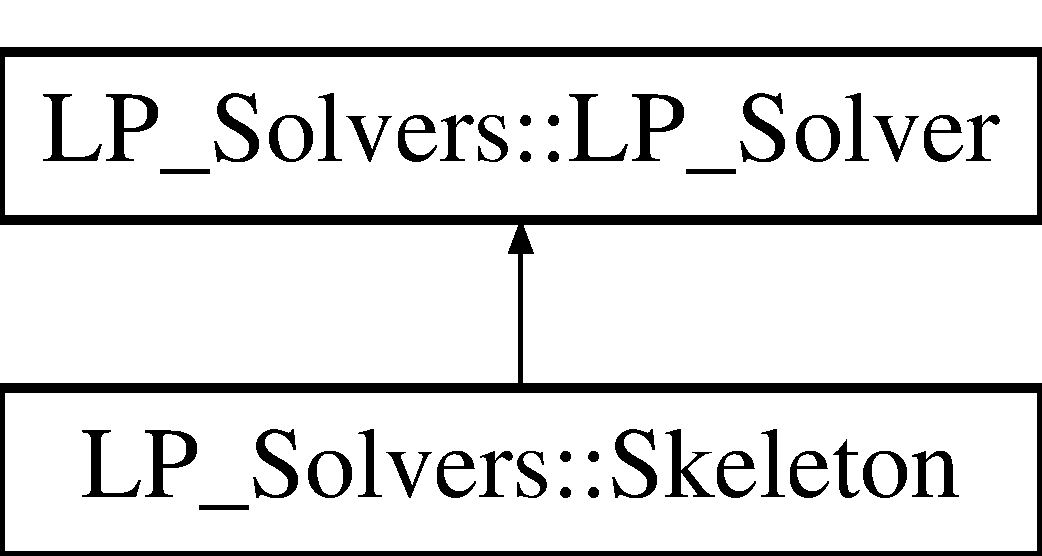
\includegraphics[height=2.000000cm]{group___c_l_s_solvers}
\end{center}
\end{figure}
\subsubsection*{Public Member Functions}
\begin{Indent}\textbf{ Construction}\par
\begin{DoxyCompactItemize}
\item 
\mbox{\Hypertarget{group___c_l_s_solvers_a10b3981d1807e86315318505ae0faeba}\label{group___c_l_s_solvers_a10b3981d1807e86315318505ae0faeba}} 
\hyperlink{group___c_l_s_solvers_a10b3981d1807e86315318505ae0faeba}{G\+L\+P\+K\+\_\+\+Solver} (N\+V\+A\+R\+\_\+\+T\+Y\+PE n)
\begin{DoxyCompactList}\small\item\em initializes solver for $ n $ variables \end{DoxyCompactList}\item 
\mbox{\Hypertarget{group___c_l_s_solvers_acdba8634513aafff25e17d42e3f8261b}\label{group___c_l_s_solvers_acdba8634513aafff25e17d42e3f8261b}} 
\hyperlink{group___c_l_s_solvers_acdba8634513aafff25e17d42e3f8261b}{G\+L\+P\+K\+\_\+\+Solver} (const \hyperlink{group___c_l_s_solvers_class_l_p___solvers_1_1_g_l_p_k___solver}{G\+L\+P\+K\+\_\+\+Solver} \&)
\begin{DoxyCompactList}\small\item\em copy constructor (deep copy) \end{DoxyCompactList}\item 
virtual bool \hyperlink{group___c_l_s_solvers_aafcda320ace4a6892704b46af99ce446}{copy} (const \hyperlink{group___c_l_s_solvers_class_l_p___solvers_1_1_l_p___solver}{L\+P\+\_\+\+Solver} $\ast$)
\begin{DoxyCompactList}\small\item\em performs a deep copy, similar to a copy constructor \end{DoxyCompactList}\end{DoxyCompactItemize}
\end{Indent}
\begin{Indent}\textbf{ Destruction}\par
\begin{DoxyCompactItemize}
\item 
\mbox{\Hypertarget{group___c_l_s_solvers_a5712c834300cea2063aa932ad8a817d7}\label{group___c_l_s_solvers_a5712c834300cea2063aa932ad8a817d7}} 
virtual {\bfseries $\sim$\+G\+L\+P\+K\+\_\+\+Solver} ()
\end{DoxyCompactItemize}
\end{Indent}
\begin{Indent}\textbf{ Basic properties}\par
\begin{DoxyCompactItemize}
\item 
\mbox{\Hypertarget{group___c_l_s_solvers_a80092baf21b7c03891f5b326a6782e52}\label{group___c_l_s_solvers_a80092baf21b7c03891f5b326a6782e52}} 
virtual N\+V\+A\+R\+\_\+\+T\+Y\+PE \hyperlink{group___c_l_s_solvers_a80092baf21b7c03891f5b326a6782e52}{get\+\_\+dimension} () const
\begin{DoxyCompactList}\small\item\em Returns the dimension of the underlying vector space. \end{DoxyCompactList}\item 
\mbox{\Hypertarget{group___c_l_s_solvers_af10b4e8c079af45803e7e76f8d00d04d}\label{group___c_l_s_solvers_af10b4e8c079af45803e7e76f8d00d04d}} 
virtual unsigned long \hyperlink{group___c_l_s_solvers_af10b4e8c079af45803e7e76f8d00d04d}{get\+\_\+number\+\_\+of\+\_\+rays} ()
\begin{DoxyCompactList}\small\item\em Returns the number of rays defining the skeleton. \end{DoxyCompactList}\item 
virtual const set$<$ \hyperlink{group___c_l_s_solvers_class_l_p___solvers_1_1_ray}{Ray} $>$ \& \hyperlink{group___c_l_s_solvers_ae011960777ca5e09d8c2b24c6ff66367}{get\+\_\+rays} ()
\begin{DoxyCompactList}\small\item\em Returns rays that define a skeleton. \end{DoxyCompactList}\item 
virtual unsigned long \hyperlink{group___c_l_s_solvers_acf743e235ac0476d8d739b139f76a0af}{get\+\_\+number\+\_\+of\+\_\+constraints} ()
\begin{DoxyCompactList}\small\item\em returns the number of constraints used by the skeleton \end{DoxyCompactList}\end{DoxyCompactItemize}
\end{Indent}
\begin{Indent}\textbf{ Modification}\par
\begin{DoxyCompactItemize}
\item 
virtual bool \hyperlink{group___c_l_s_solvers_a544cb09dfa211fae9adaacfd402af9a2}{solve} (const \hyperlink{group___c_l_s_solvers_class_l_p___solvers_1_1_constraint}{Constraint} \&)
\begin{DoxyCompactList}\small\item\em Adds the indicated constraint (singular!) and re-\/computes the solution. \end{DoxyCompactList}\item 
virtual bool \hyperlink{group___c_l_s_solvers_a1ceccb6fc4eff73cc4237c46ab9e7699}{solve} (const vector$<$ \hyperlink{group___c_l_s_solvers_class_l_p___solvers_1_1_constraint}{Constraint} $>$ \&)
\begin{DoxyCompactList}\small\item\em Adds the indicated constraints (plural!) and re-\/computes the solution. \end{DoxyCompactList}\end{DoxyCompactItemize}
\end{Indent}
\begin{Indent}\textbf{ Computation}\par
\begin{DoxyCompactItemize}
\item 
\mbox{\Hypertarget{group___c_l_s_solvers_a1c395efc09c537d49911656155487213}\label{group___c_l_s_solvers_a1c395efc09c537d49911656155487213}} 
virtual bool \hyperlink{group___c_l_s_solvers_a1c395efc09c537d49911656155487213}{makes\+\_\+consistent\+\_\+constraint} (const \hyperlink{group__polygroup_class_monomial}{Monomial} \&t, const \hyperlink{group__polygroup_class_monomial}{Monomial} \&u, bool show\+\_\+data=false)
\begin{DoxyCompactList}\small\item\em tests for consistency of a constraint generated by two monomials. \end{DoxyCompactList}\end{DoxyCompactItemize}
\end{Indent}
\subsection*{Additional Inherited Members}


\paragraph{Member Function Documentation}
\mbox{\Hypertarget{group___c_l_s_solvers_aafcda320ace4a6892704b46af99ce446}\label{group___c_l_s_solvers_aafcda320ace4a6892704b46af99ce446}} 
\index{L\+P\+\_\+\+Solvers\+::\+G\+L\+P\+K\+\_\+\+Solver@{L\+P\+\_\+\+Solvers\+::\+G\+L\+P\+K\+\_\+\+Solver}!copy@{copy}}
\index{copy@{copy}!L\+P\+\_\+\+Solvers\+::\+G\+L\+P\+K\+\_\+\+Solver@{L\+P\+\_\+\+Solvers\+::\+G\+L\+P\+K\+\_\+\+Solver}}
\subparagraph{\texorpdfstring{copy()}{copy()}}
{\footnotesize\ttfamily bool L\+P\+\_\+\+Solvers\+::\+G\+L\+P\+K\+\_\+\+Solver\+::copy (\begin{DoxyParamCaption}\item[{const \hyperlink{group___c_l_s_solvers_class_l_p___solvers_1_1_l_p___solver}{L\+P\+\_\+\+Solver} $\ast$}]{ }\end{DoxyParamCaption})\hspace{0.3cm}{\ttfamily [virtual]}}



performs a deep copy, similar to a copy constructor 

\begin{DoxyReturn}{Returns}
{\ttfamily true} iff copying was successful 
\end{DoxyReturn}
\begin{DoxyWarning}{Warning}
Do not mix-\/and-\/match solvers. At the present time, a \hyperlink{group___c_l_s_solvers_class_l_p___solvers_1_1_p_p_l___solver}{P\+P\+L\+\_\+\+Solver} is not equipped to copy a \hyperlink{group___c_l_s_solvers_class_l_p___solvers_1_1_g_l_p_k___solver}{G\+L\+P\+K\+\_\+\+Solver}, or vice versa. (This doesn\textquotesingle{}t even make sense between exact and approximate solvers.) 
\end{DoxyWarning}


Implements \hyperlink{group___c_l_s_solvers_a36c14a88e9d3ae9d9321acc7877236d0}{L\+P\+\_\+\+Solvers\+::\+L\+P\+\_\+\+Solver}.



Definition at line 60 of file glpk\+\_\+solver.\+cpp.

\mbox{\Hypertarget{group___c_l_s_solvers_acf743e235ac0476d8d739b139f76a0af}\label{group___c_l_s_solvers_acf743e235ac0476d8d739b139f76a0af}} 
\index{L\+P\+\_\+\+Solvers\+::\+G\+L\+P\+K\+\_\+\+Solver@{L\+P\+\_\+\+Solvers\+::\+G\+L\+P\+K\+\_\+\+Solver}!get\+\_\+number\+\_\+of\+\_\+constraints@{get\+\_\+number\+\_\+of\+\_\+constraints}}
\index{get\+\_\+number\+\_\+of\+\_\+constraints@{get\+\_\+number\+\_\+of\+\_\+constraints}!L\+P\+\_\+\+Solvers\+::\+G\+L\+P\+K\+\_\+\+Solver@{L\+P\+\_\+\+Solvers\+::\+G\+L\+P\+K\+\_\+\+Solver}}
\subparagraph{\texorpdfstring{get\+\_\+number\+\_\+of\+\_\+constraints()}{get\_number\_of\_constraints()}}
{\footnotesize\ttfamily virtual unsigned long L\+P\+\_\+\+Solvers\+::\+G\+L\+P\+K\+\_\+\+Solver\+::get\+\_\+number\+\_\+of\+\_\+constraints (\begin{DoxyParamCaption}{ }\end{DoxyParamCaption})\hspace{0.3cm}{\ttfamily [inline]}, {\ttfamily [virtual]}}



returns the number of constraints used by the skeleton 

\begin{DoxyReturn}{Returns}
number of constraints 
\end{DoxyReturn}


Implements \hyperlink{group___c_l_s_solvers_a05697a4527b15e26b5e0ae9088a46ed5}{L\+P\+\_\+\+Solvers\+::\+L\+P\+\_\+\+Solver}.



Definition at line 63 of file glpk\+\_\+solver.\+hpp.

\mbox{\Hypertarget{group___c_l_s_solvers_ae011960777ca5e09d8c2b24c6ff66367}\label{group___c_l_s_solvers_ae011960777ca5e09d8c2b24c6ff66367}} 
\index{L\+P\+\_\+\+Solvers\+::\+G\+L\+P\+K\+\_\+\+Solver@{L\+P\+\_\+\+Solvers\+::\+G\+L\+P\+K\+\_\+\+Solver}!get\+\_\+rays@{get\+\_\+rays}}
\index{get\+\_\+rays@{get\+\_\+rays}!L\+P\+\_\+\+Solvers\+::\+G\+L\+P\+K\+\_\+\+Solver@{L\+P\+\_\+\+Solvers\+::\+G\+L\+P\+K\+\_\+\+Solver}}
\subparagraph{\texorpdfstring{get\+\_\+rays()}{get\_rays()}}
{\footnotesize\ttfamily const set$<$ \hyperlink{group___c_l_s_solvers_class_l_p___solvers_1_1_ray}{Ray} $>$ \& L\+P\+\_\+\+Solvers\+::\+G\+L\+P\+K\+\_\+\+Solver\+::get\+\_\+rays (\begin{DoxyParamCaption}{ }\end{DoxyParamCaption})\hspace{0.3cm}{\ttfamily [virtual]}}



Returns rays that define a skeleton. 

\begin{DoxyReturn}{Returns}
a set of \hyperlink{group___c_l_s_solvers_class_l_p___solvers_1_1_ray}{Ray} that define the given skeleton
\end{DoxyReturn}
When using an approximate solver such as \hyperlink{group___c_l_s_solvers_class_l_p___solvers_1_1_g_l_p_k___solver}{G\+L\+P\+K\+\_\+\+Solver}, this will give only an approximate skeleton. 

Reimplemented from \hyperlink{group___c_l_s_solvers_a52f7a4068e9d36500d1dcdf35757cd06}{L\+P\+\_\+\+Solvers\+::\+L\+P\+\_\+\+Solver}.



Definition at line 144 of file glpk\+\_\+solver.\+cpp.

\mbox{\Hypertarget{group___c_l_s_solvers_a544cb09dfa211fae9adaacfd402af9a2}\label{group___c_l_s_solvers_a544cb09dfa211fae9adaacfd402af9a2}} 
\index{L\+P\+\_\+\+Solvers\+::\+G\+L\+P\+K\+\_\+\+Solver@{L\+P\+\_\+\+Solvers\+::\+G\+L\+P\+K\+\_\+\+Solver}!solve@{solve}}
\index{solve@{solve}!L\+P\+\_\+\+Solvers\+::\+G\+L\+P\+K\+\_\+\+Solver@{L\+P\+\_\+\+Solvers\+::\+G\+L\+P\+K\+\_\+\+Solver}}
\subparagraph{\texorpdfstring{solve()}{solve()}\hspace{0.1cm}{\footnotesize\ttfamily [1/2]}}
{\footnotesize\ttfamily bool L\+P\+\_\+\+Solvers\+::\+G\+L\+P\+K\+\_\+\+Solver\+::solve (\begin{DoxyParamCaption}\item[{const \hyperlink{group___c_l_s_solvers_class_l_p___solvers_1_1_constraint}{Constraint} \&}]{ }\end{DoxyParamCaption})\hspace{0.3cm}{\ttfamily [virtual]}}



Adds the indicated constraint (singular!) and re-\/computes the solution. 

\begin{DoxyReturn}{Returns}
{\ttfamily true} if and only if the new constraint is consistent with the current constraints
\end{DoxyReturn}
\begin{DoxyWarning}{Warning}
Checking the return value is crucial! If the function returns {\ttfamily false}, you have an inconsistent system! While the {\itshape present} cone will remain consistent, {\bfseries the function will not roll back previous changes you have made}, so if you want to iterate again, your best bet is to copy the skeleton, and try that copy. Accept the new constraints only if that copy succeeds, in which case, you might as well discard the original, and keep the copy. 
\end{DoxyWarning}


Implements \hyperlink{group___c_l_s_solvers_a8b9979fb228ac9ccfe037ad6ca48b314}{L\+P\+\_\+\+Solvers\+::\+L\+P\+\_\+\+Solver}.



Definition at line 118 of file glpk\+\_\+solver.\+cpp.

\mbox{\Hypertarget{group___c_l_s_solvers_a1ceccb6fc4eff73cc4237c46ab9e7699}\label{group___c_l_s_solvers_a1ceccb6fc4eff73cc4237c46ab9e7699}} 
\index{L\+P\+\_\+\+Solvers\+::\+G\+L\+P\+K\+\_\+\+Solver@{L\+P\+\_\+\+Solvers\+::\+G\+L\+P\+K\+\_\+\+Solver}!solve@{solve}}
\index{solve@{solve}!L\+P\+\_\+\+Solvers\+::\+G\+L\+P\+K\+\_\+\+Solver@{L\+P\+\_\+\+Solvers\+::\+G\+L\+P\+K\+\_\+\+Solver}}
\subparagraph{\texorpdfstring{solve()}{solve()}\hspace{0.1cm}{\footnotesize\ttfamily [2/2]}}
{\footnotesize\ttfamily bool L\+P\+\_\+\+Solvers\+::\+G\+L\+P\+K\+\_\+\+Solver\+::solve (\begin{DoxyParamCaption}\item[{const vector$<$ \hyperlink{group___c_l_s_solvers_class_l_p___solvers_1_1_constraint}{Constraint} $>$ \&}]{ }\end{DoxyParamCaption})\hspace{0.3cm}{\ttfamily [virtual]}}



Adds the indicated constraints (plural!) and re-\/computes the solution. 

\begin{DoxyReturn}{Returns}
{\ttfamily true} if and only if the new constraints are consistent with the current constraints
\end{DoxyReturn}
\begin{DoxyWarning}{Warning}
Checking the return value is crucial! If the function returns {\ttfamily false}, you have an inconsistent system! While the {\itshape present} cone will remain consistent, {\bfseries the function will not roll back previous changes you have made}, so if you want to iterate again, your best bet is to copy the skeleton, and try that copy. Accept the new constraints only if that copy succeeds, in which case, you might as well discard the original, and keep the copy. 
\end{DoxyWarning}


Implements \hyperlink{group___c_l_s_solvers_aea1a5bf98a2c4c06b0550cacdf8b88fd}{L\+P\+\_\+\+Solvers\+::\+L\+P\+\_\+\+Solver}.



Definition at line 87 of file glpk\+\_\+solver.\+cpp.

\index{L\+P\+\_\+\+Solvers\+::\+L\+P\+\_\+\+Solver@{L\+P\+\_\+\+Solvers\+::\+L\+P\+\_\+\+Solver}}\label{class_l_p___solvers_1_1_l_p___solver}
\Hypertarget{group___c_l_s_solvers_class_l_p___solvers_1_1_l_p___solver}
\subsubsection{class L\+P\+\_\+\+Solvers\+:\+:L\+P\+\_\+\+Solver}
exact or approximate polyhedral cone solution, with methods allowing definition and refinement 

\begin{DoxyAuthor}{Author}
John Perry 
\end{DoxyAuthor}
\begin{DoxyVersion}{Version}
1.\+0 
\end{DoxyVersion}
\begin{DoxyDate}{Date}
January 2017 
\end{DoxyDate}
\begin{DoxyCopyright}{Copyright}
The University of Southern Mississippi
\end{DoxyCopyright}
This class encapsulates the skeleton of a polyhedral cone, defined by a sequence of inequalities of the form $ c_1 x_1 + \cdots c_n x_n \geq 0 $.

\begin{DoxyWarning}{Warning}
Some classes may provide only an {\itshape approximate} cone; see, for example, \hyperlink{group___c_l_s_solvers_class_l_p___solvers_1_1_g_l_p_k___solver}{G\+L\+P\+K\+\_\+\+Solver}. In addition, Clients must ensure two things.
\begin{DoxyEnumerate}
\item The rays must have the same number $ m $ of dimensions, constraints must have the same number $ n $ of variables, and $ m=n $. Violating any of these three conditions will lead to undesirable behavior.
\item When refining the cone, it is essential to check that the return value of \hyperlink{group___c_l_s_solvers_a8b9979fb228ac9ccfe037ad6ca48b314}{solve()} is {\ttfamily true}; for if it is not, then the cone is no longer be consistent. Please read the relevant documentation. 
\end{DoxyEnumerate}
\end{DoxyWarning}


Definition at line 564 of file lp\+\_\+solver.\+hpp.

Inheritance diagram for L\+P\+\_\+\+Solvers\+:\+:L\+P\+\_\+\+Solver\+:\begin{figure}[H]
\begin{center}
\leavevmode
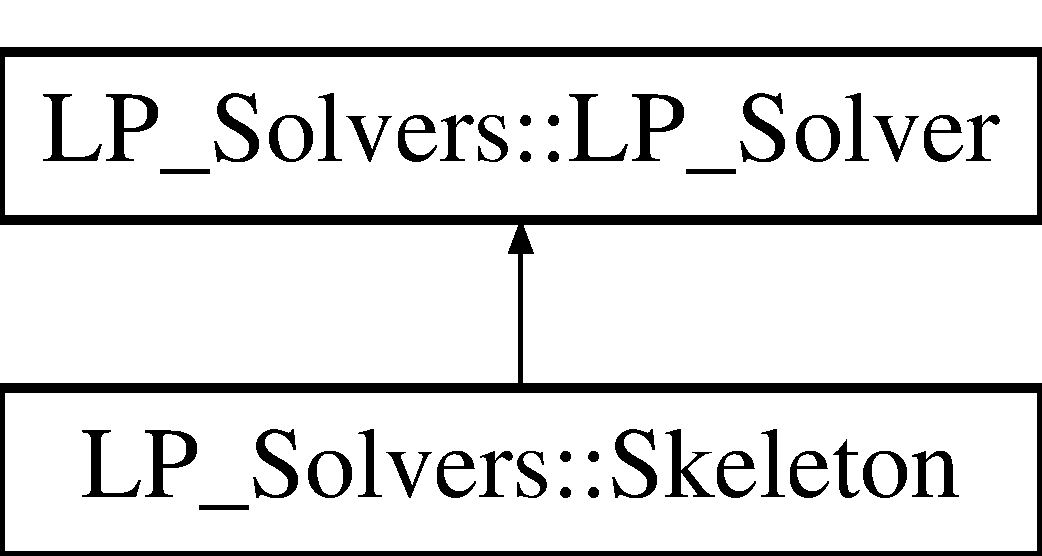
\includegraphics[height=2.000000cm]{group___c_l_s_solvers}
\end{center}
\end{figure}
\subsubsection*{Public Member Functions}
\begin{Indent}\textbf{ Construction}\par
\begin{DoxyCompactItemize}
\item 
virtual bool \hyperlink{group___c_l_s_solvers_a36c14a88e9d3ae9d9321acc7877236d0}{copy} (const \hyperlink{group___c_l_s_solvers_class_l_p___solvers_1_1_l_p___solver}{L\+P\+\_\+\+Solver} $\ast$)=0
\begin{DoxyCompactList}\small\item\em performs a deep copy, similar to a copy constructor \end{DoxyCompactList}\end{DoxyCompactItemize}
\end{Indent}
\begin{Indent}\textbf{ Destruction}\par
\begin{DoxyCompactItemize}
\item 
\mbox{\Hypertarget{group___c_l_s_solvers_a1d530b23b2516c36cbc02173e667d0cf}\label{group___c_l_s_solvers_a1d530b23b2516c36cbc02173e667d0cf}} 
virtual \hyperlink{group___c_l_s_solvers_a1d530b23b2516c36cbc02173e667d0cf}{$\sim$\+L\+P\+\_\+\+Solver} ()
\begin{DoxyCompactList}\small\item\em the default destructor does nothing (this is an abstract class) \end{DoxyCompactList}\end{DoxyCompactItemize}
\end{Indent}
\begin{Indent}\textbf{ Modification}\par
\begin{DoxyCompactItemize}
\item 
virtual bool \hyperlink{group___c_l_s_solvers_a8b9979fb228ac9ccfe037ad6ca48b314}{solve} (const \hyperlink{group___c_l_s_solvers_class_l_p___solvers_1_1_constraint}{Constraint} \&)=0
\begin{DoxyCompactList}\small\item\em Adds the indicated constraint (singular!) and re-\/computes the solution. \end{DoxyCompactList}\item 
virtual bool \hyperlink{group___c_l_s_solvers_aea1a5bf98a2c4c06b0550cacdf8b88fd}{solve} (const vector$<$ \hyperlink{group___c_l_s_solvers_class_l_p___solvers_1_1_constraint}{Constraint} $>$ \&)=0
\begin{DoxyCompactList}\small\item\em Adds the indicated constraints (plural!) and re-\/computes the solution. \end{DoxyCompactList}\end{DoxyCompactItemize}
\end{Indent}
\begin{Indent}\textbf{ Basic properies}\par
\begin{DoxyCompactItemize}
\item 
\mbox{\Hypertarget{group___c_l_s_solvers_a5801b4bd5322a78e0cf3dcad83383a2e}\label{group___c_l_s_solvers_a5801b4bd5322a78e0cf3dcad83383a2e}} 
virtual N\+V\+A\+R\+\_\+\+T\+Y\+PE \hyperlink{group___c_l_s_solvers_a5801b4bd5322a78e0cf3dcad83383a2e}{get\+\_\+dimension} () const =0
\begin{DoxyCompactList}\small\item\em Returns the dimension of the underlying vector space. \end{DoxyCompactList}\item 
\mbox{\Hypertarget{group___c_l_s_solvers_a7a8d455722e6ae8b0bc9928dcd1bfa48}\label{group___c_l_s_solvers_a7a8d455722e6ae8b0bc9928dcd1bfa48}} 
virtual unsigned long \hyperlink{group___c_l_s_solvers_a7a8d455722e6ae8b0bc9928dcd1bfa48}{get\+\_\+number\+\_\+of\+\_\+rays} ()
\begin{DoxyCompactList}\small\item\em Returns the number of rays defining the skeleton. \end{DoxyCompactList}\item 
virtual const set$<$ \hyperlink{group___c_l_s_solvers_class_l_p___solvers_1_1_ray}{Ray} $>$ \& \hyperlink{group___c_l_s_solvers_a52f7a4068e9d36500d1dcdf35757cd06}{get\+\_\+rays} ()
\begin{DoxyCompactList}\small\item\em Returns rays that define a skeleton. \end{DoxyCompactList}\item 
virtual unsigned long \hyperlink{group___c_l_s_solvers_a05697a4527b15e26b5e0ae9088a46ed5}{get\+\_\+number\+\_\+of\+\_\+constraints} ()=0
\begin{DoxyCompactList}\small\item\em returns the number of constraints used by the skeleton \end{DoxyCompactList}\end{DoxyCompactItemize}
\end{Indent}
\begin{Indent}\textbf{ Computation}\par
\begin{DoxyCompactItemize}
\item 
\mbox{\Hypertarget{group___c_l_s_solvers_abb6c3f1320ea90c0a81960642a503b37}\label{group___c_l_s_solvers_abb6c3f1320ea90c0a81960642a503b37}} 
virtual bool \hyperlink{group___c_l_s_solvers_abb6c3f1320ea90c0a81960642a503b37}{makes\+\_\+consistent\+\_\+constraint} (const \hyperlink{group__polygroup_class_monomial}{Monomial} \&t, const \hyperlink{group__polygroup_class_monomial}{Monomial} \&u, bool show\+\_\+data=false)
\begin{DoxyCompactList}\small\item\em tests for consistency of a constraint generated by two monomials. \end{DoxyCompactList}\end{DoxyCompactItemize}
\end{Indent}
\subsubsection*{Protected Attributes}
\begin{DoxyCompactItemize}
\item 
set$<$ \hyperlink{group___c_l_s_solvers_class_l_p___solvers_1_1_ray}{Ray} $>$ \hyperlink{group___c_l_s_solvers_ad4c9fb3708c156496c23515c8e841374}{rays}
\end{DoxyCompactItemize}


\paragraph{Member Function Documentation}
\mbox{\Hypertarget{group___c_l_s_solvers_a36c14a88e9d3ae9d9321acc7877236d0}\label{group___c_l_s_solvers_a36c14a88e9d3ae9d9321acc7877236d0}} 
\index{L\+P\+\_\+\+Solvers\+::\+L\+P\+\_\+\+Solver@{L\+P\+\_\+\+Solvers\+::\+L\+P\+\_\+\+Solver}!copy@{copy}}
\index{copy@{copy}!L\+P\+\_\+\+Solvers\+::\+L\+P\+\_\+\+Solver@{L\+P\+\_\+\+Solvers\+::\+L\+P\+\_\+\+Solver}}
\subparagraph{\texorpdfstring{copy()}{copy()}}
{\footnotesize\ttfamily virtual bool L\+P\+\_\+\+Solvers\+::\+L\+P\+\_\+\+Solver\+::copy (\begin{DoxyParamCaption}\item[{const \hyperlink{group___c_l_s_solvers_class_l_p___solvers_1_1_l_p___solver}{L\+P\+\_\+\+Solver} $\ast$}]{ }\end{DoxyParamCaption})\hspace{0.3cm}{\ttfamily [pure virtual]}}



performs a deep copy, similar to a copy constructor 

\begin{DoxyReturn}{Returns}
{\ttfamily true} iff copying was successful 
\end{DoxyReturn}
\begin{DoxyWarning}{Warning}
Do not mix-\/and-\/match solvers. At the present time, a \hyperlink{group___c_l_s_solvers_class_l_p___solvers_1_1_p_p_l___solver}{P\+P\+L\+\_\+\+Solver} is not equipped to copy a \hyperlink{group___c_l_s_solvers_class_l_p___solvers_1_1_g_l_p_k___solver}{G\+L\+P\+K\+\_\+\+Solver}, or vice versa. (This doesn\textquotesingle{}t even make sense between exact and approximate solvers.) 
\end{DoxyWarning}


Implemented in \hyperlink{group___c_l_s_solvers_a33b1747069c512ad69e30cb0c8786577}{L\+P\+\_\+\+Solvers\+::\+Skeleton}, \hyperlink{group___c_l_s_solvers_aa447a576420597eb9ff86b8875f5d30c}{L\+P\+\_\+\+Solvers\+::\+P\+P\+L\+\_\+\+Solver}, and \hyperlink{group___c_l_s_solvers_aafcda320ace4a6892704b46af99ce446}{L\+P\+\_\+\+Solvers\+::\+G\+L\+P\+K\+\_\+\+Solver}.

\mbox{\Hypertarget{group___c_l_s_solvers_a05697a4527b15e26b5e0ae9088a46ed5}\label{group___c_l_s_solvers_a05697a4527b15e26b5e0ae9088a46ed5}} 
\index{L\+P\+\_\+\+Solvers\+::\+L\+P\+\_\+\+Solver@{L\+P\+\_\+\+Solvers\+::\+L\+P\+\_\+\+Solver}!get\+\_\+number\+\_\+of\+\_\+constraints@{get\+\_\+number\+\_\+of\+\_\+constraints}}
\index{get\+\_\+number\+\_\+of\+\_\+constraints@{get\+\_\+number\+\_\+of\+\_\+constraints}!L\+P\+\_\+\+Solvers\+::\+L\+P\+\_\+\+Solver@{L\+P\+\_\+\+Solvers\+::\+L\+P\+\_\+\+Solver}}
\subparagraph{\texorpdfstring{get\+\_\+number\+\_\+of\+\_\+constraints()}{get\_number\_of\_constraints()}}
{\footnotesize\ttfamily virtual unsigned long L\+P\+\_\+\+Solvers\+::\+L\+P\+\_\+\+Solver\+::get\+\_\+number\+\_\+of\+\_\+constraints (\begin{DoxyParamCaption}{ }\end{DoxyParamCaption})\hspace{0.3cm}{\ttfamily [pure virtual]}}



returns the number of constraints used by the skeleton 

\begin{DoxyReturn}{Returns}
number of constraints 
\end{DoxyReturn}


Implemented in \hyperlink{group___c_l_s_solvers_a1fcb6873ce96085aa68f97064cd90c9d}{L\+P\+\_\+\+Solvers\+::\+Skeleton}, \hyperlink{group___c_l_s_solvers_acf743e235ac0476d8d739b139f76a0af}{L\+P\+\_\+\+Solvers\+::\+G\+L\+P\+K\+\_\+\+Solver}, and \hyperlink{group___c_l_s_solvers_a8c8dbe226a971e62159888aecacce458}{L\+P\+\_\+\+Solvers\+::\+P\+P\+L\+\_\+\+Solver}.

\mbox{\Hypertarget{group___c_l_s_solvers_a52f7a4068e9d36500d1dcdf35757cd06}\label{group___c_l_s_solvers_a52f7a4068e9d36500d1dcdf35757cd06}} 
\index{L\+P\+\_\+\+Solvers\+::\+L\+P\+\_\+\+Solver@{L\+P\+\_\+\+Solvers\+::\+L\+P\+\_\+\+Solver}!get\+\_\+rays@{get\+\_\+rays}}
\index{get\+\_\+rays@{get\+\_\+rays}!L\+P\+\_\+\+Solvers\+::\+L\+P\+\_\+\+Solver@{L\+P\+\_\+\+Solvers\+::\+L\+P\+\_\+\+Solver}}
\subparagraph{\texorpdfstring{get\+\_\+rays()}{get\_rays()}}
{\footnotesize\ttfamily const set$<$ \hyperlink{group___c_l_s_solvers_class_l_p___solvers_1_1_ray}{Ray} $>$ \& L\+P\+\_\+\+Solvers\+::\+L\+P\+\_\+\+Solver\+::get\+\_\+rays (\begin{DoxyParamCaption}{ }\end{DoxyParamCaption})\hspace{0.3cm}{\ttfamily [virtual]}}



Returns rays that define a skeleton. 

\begin{DoxyReturn}{Returns}
a set of \hyperlink{group___c_l_s_solvers_class_l_p___solvers_1_1_ray}{Ray} that define the given skeleton
\end{DoxyReturn}
When using an approximate solver such as \hyperlink{group___c_l_s_solvers_class_l_p___solvers_1_1_g_l_p_k___solver}{G\+L\+P\+K\+\_\+\+Solver}, this will give only an approximate skeleton. 

Reimplemented in \hyperlink{group___c_l_s_solvers_ae011960777ca5e09d8c2b24c6ff66367}{L\+P\+\_\+\+Solvers\+::\+G\+L\+P\+K\+\_\+\+Solver}.



Definition at line 380 of file lp\+\_\+solver.\+cpp.

\mbox{\Hypertarget{group___c_l_s_solvers_a8b9979fb228ac9ccfe037ad6ca48b314}\label{group___c_l_s_solvers_a8b9979fb228ac9ccfe037ad6ca48b314}} 
\index{L\+P\+\_\+\+Solvers\+::\+L\+P\+\_\+\+Solver@{L\+P\+\_\+\+Solvers\+::\+L\+P\+\_\+\+Solver}!solve@{solve}}
\index{solve@{solve}!L\+P\+\_\+\+Solvers\+::\+L\+P\+\_\+\+Solver@{L\+P\+\_\+\+Solvers\+::\+L\+P\+\_\+\+Solver}}
\subparagraph{\texorpdfstring{solve()}{solve()}\hspace{0.1cm}{\footnotesize\ttfamily [1/2]}}
{\footnotesize\ttfamily virtual bool L\+P\+\_\+\+Solvers\+::\+L\+P\+\_\+\+Solver\+::solve (\begin{DoxyParamCaption}\item[{const \hyperlink{group___c_l_s_solvers_class_l_p___solvers_1_1_constraint}{Constraint} \&}]{ }\end{DoxyParamCaption})\hspace{0.3cm}{\ttfamily [pure virtual]}}



Adds the indicated constraint (singular!) and re-\/computes the solution. 

\begin{DoxyReturn}{Returns}
{\ttfamily true} if and only if the new constraint is consistent with the current constraints
\end{DoxyReturn}
\begin{DoxyWarning}{Warning}
Checking the return value is crucial! If the function returns {\ttfamily false}, you have an inconsistent system! While the {\itshape present} cone will remain consistent, {\bfseries the function will not roll back previous changes you have made}, so if you want to iterate again, your best bet is to copy the skeleton, and try that copy. Accept the new constraints only if that copy succeeds, in which case, you might as well discard the original, and keep the copy. 
\end{DoxyWarning}


Implemented in \hyperlink{group___c_l_s_solvers_a202b0b37e0ea8a817ce6e29c93a39cd8}{L\+P\+\_\+\+Solvers\+::\+Skeleton}, \hyperlink{group___c_l_s_solvers_a544cb09dfa211fae9adaacfd402af9a2}{L\+P\+\_\+\+Solvers\+::\+G\+L\+P\+K\+\_\+\+Solver}, and \hyperlink{group___c_l_s_solvers_affe1dce30ec7bad7c54e4edf9283235e}{L\+P\+\_\+\+Solvers\+::\+P\+P\+L\+\_\+\+Solver}.

\mbox{\Hypertarget{group___c_l_s_solvers_aea1a5bf98a2c4c06b0550cacdf8b88fd}\label{group___c_l_s_solvers_aea1a5bf98a2c4c06b0550cacdf8b88fd}} 
\index{L\+P\+\_\+\+Solvers\+::\+L\+P\+\_\+\+Solver@{L\+P\+\_\+\+Solvers\+::\+L\+P\+\_\+\+Solver}!solve@{solve}}
\index{solve@{solve}!L\+P\+\_\+\+Solvers\+::\+L\+P\+\_\+\+Solver@{L\+P\+\_\+\+Solvers\+::\+L\+P\+\_\+\+Solver}}
\subparagraph{\texorpdfstring{solve()}{solve()}\hspace{0.1cm}{\footnotesize\ttfamily [2/2]}}
{\footnotesize\ttfamily virtual bool L\+P\+\_\+\+Solvers\+::\+L\+P\+\_\+\+Solver\+::solve (\begin{DoxyParamCaption}\item[{const vector$<$ \hyperlink{group___c_l_s_solvers_class_l_p___solvers_1_1_constraint}{Constraint} $>$ \&}]{ }\end{DoxyParamCaption})\hspace{0.3cm}{\ttfamily [pure virtual]}}



Adds the indicated constraints (plural!) and re-\/computes the solution. 

\begin{DoxyReturn}{Returns}
{\ttfamily true} if and only if the new constraints are consistent with the current constraints
\end{DoxyReturn}
\begin{DoxyWarning}{Warning}
Checking the return value is crucial! If the function returns {\ttfamily false}, you have an inconsistent system! While the {\itshape present} cone will remain consistent, {\bfseries the function will not roll back previous changes you have made}, so if you want to iterate again, your best bet is to copy the skeleton, and try that copy. Accept the new constraints only if that copy succeeds, in which case, you might as well discard the original, and keep the copy. 
\end{DoxyWarning}


Implemented in \hyperlink{group___c_l_s_solvers_aba082a338a2cb3ace612fd2dfba667c5}{L\+P\+\_\+\+Solvers\+::\+Skeleton}, \hyperlink{group___c_l_s_solvers_a1ceccb6fc4eff73cc4237c46ab9e7699}{L\+P\+\_\+\+Solvers\+::\+G\+L\+P\+K\+\_\+\+Solver}, and \hyperlink{group___c_l_s_solvers_a6f73ee7b0d42f78fd95e399c474b3eb4}{L\+P\+\_\+\+Solvers\+::\+P\+P\+L\+\_\+\+Solver}.



\paragraph{Member Data Documentation}
\mbox{\Hypertarget{group___c_l_s_solvers_ad4c9fb3708c156496c23515c8e841374}\label{group___c_l_s_solvers_ad4c9fb3708c156496c23515c8e841374}} 
\index{L\+P\+\_\+\+Solvers\+::\+L\+P\+\_\+\+Solver@{L\+P\+\_\+\+Solvers\+::\+L\+P\+\_\+\+Solver}!rays@{rays}}
\index{rays@{rays}!L\+P\+\_\+\+Solvers\+::\+L\+P\+\_\+\+Solver@{L\+P\+\_\+\+Solvers\+::\+L\+P\+\_\+\+Solver}}
\subparagraph{\texorpdfstring{rays}{rays}}
{\footnotesize\ttfamily set$<$\hyperlink{group___c_l_s_solvers_class_l_p___solvers_1_1_ray}{Ray}$>$ L\+P\+\_\+\+Solvers\+::\+L\+P\+\_\+\+Solver\+::rays\hspace{0.3cm}{\ttfamily [protected]}}

the skeleton (may be approximate, depending on solver) 

Definition at line 666 of file lp\+\_\+solver.\+hpp.

\index{L\+P\+\_\+\+Solvers\+::\+P\+P\+L\+\_\+\+Solver@{L\+P\+\_\+\+Solvers\+::\+P\+P\+L\+\_\+\+Solver}}\label{class_l_p___solvers_1_1_p_p_l___solver}
\Hypertarget{group___c_l_s_solvers_class_l_p___solvers_1_1_p_p_l___solver}
\subsubsection{class L\+P\+\_\+\+Solvers\+:\+:P\+P\+L\+\_\+\+Solver}
approximate skeleton of a polyhedral cone, using P\+PL linear solver 

\begin{DoxyAuthor}{Author}
John Perry 
\end{DoxyAuthor}
\begin{DoxyVersion}{Version}
1.\+0 
\end{DoxyVersion}
\begin{DoxyDate}{Date}
January 2017 
\end{DoxyDate}
\begin{DoxyCopyright}{Copyright}
The University of Southern Mississippi
\end{DoxyCopyright}
This class serves as an interface to P\+PL \cite{BagnaraHZ08SCP}, which we can use to find the skeleton to a polyhedral cone. 

Definition at line 40 of file ppl\+\_\+solver.\+hpp.

Inheritance diagram for L\+P\+\_\+\+Solvers\+:\+:P\+P\+L\+\_\+\+Solver\+:\begin{figure}[H]
\begin{center}
\leavevmode
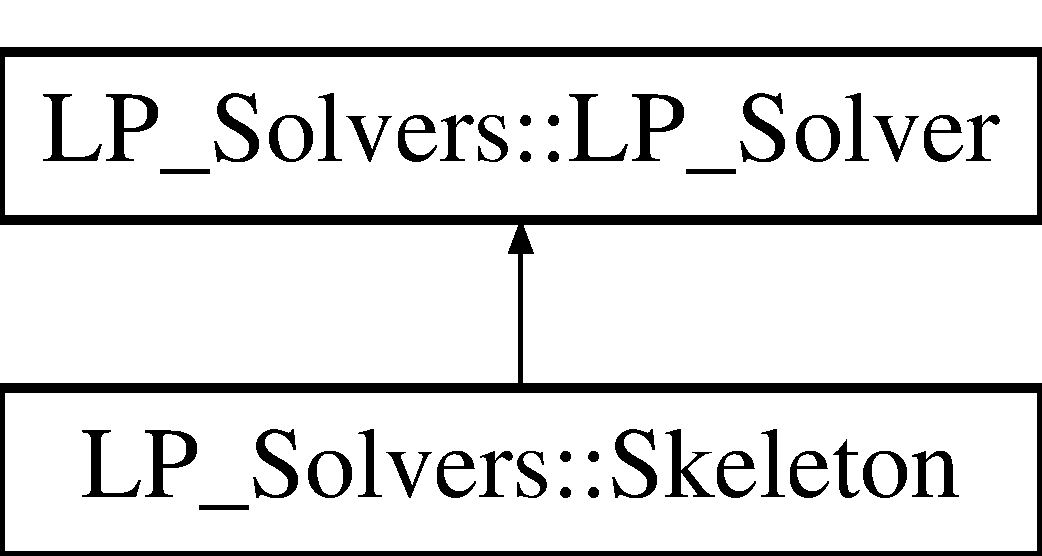
\includegraphics[height=2.000000cm]{group___c_l_s_solvers}
\end{center}
\end{figure}
\subsubsection*{Public Member Functions}
\begin{Indent}\textbf{ Construction}\par
\begin{DoxyCompactItemize}
\item 
\mbox{\Hypertarget{group___c_l_s_solvers_a8676ceed54fc8883fd0c2cab45e7d9a4}\label{group___c_l_s_solvers_a8676ceed54fc8883fd0c2cab45e7d9a4}} 
\hyperlink{group___c_l_s_solvers_a8676ceed54fc8883fd0c2cab45e7d9a4}{P\+P\+L\+\_\+\+Solver} (N\+V\+A\+R\+\_\+\+T\+Y\+PE \hyperlink{group___c_l_s_solvers_a10d4394603a6a565a95fc65ce0f9a172}{n})
\begin{DoxyCompactList}\small\item\em initializes solver for $ n $ variables \end{DoxyCompactList}\item 
\mbox{\Hypertarget{group___c_l_s_solvers_a53d5564f046f82f07f58e557228f10c5}\label{group___c_l_s_solvers_a53d5564f046f82f07f58e557228f10c5}} 
\hyperlink{group___c_l_s_solvers_a53d5564f046f82f07f58e557228f10c5}{P\+P\+L\+\_\+\+Solver} (const \hyperlink{group___c_l_s_solvers_class_l_p___solvers_1_1_p_p_l___solver}{P\+P\+L\+\_\+\+Solver} \&)
\begin{DoxyCompactList}\small\item\em copy constructor (deep copy) \end{DoxyCompactList}\item 
virtual bool \hyperlink{group___c_l_s_solvers_aa447a576420597eb9ff86b8875f5d30c}{copy} (const \hyperlink{group___c_l_s_solvers_class_l_p___solvers_1_1_l_p___solver}{L\+P\+\_\+\+Solver} $\ast$)
\begin{DoxyCompactList}\small\item\em performs a deep copy, similar to a copy constructor \end{DoxyCompactList}\end{DoxyCompactItemize}
\end{Indent}
\begin{Indent}\textbf{ Destruction}\par
\begin{DoxyCompactItemize}
\item 
\mbox{\Hypertarget{group___c_l_s_solvers_a2d4cd90b9e8bab2ff0fe3178bb894e75}\label{group___c_l_s_solvers_a2d4cd90b9e8bab2ff0fe3178bb894e75}} 
virtual {\bfseries $\sim$\+P\+P\+L\+\_\+\+Solver} ()
\end{DoxyCompactItemize}
\end{Indent}
\begin{Indent}\textbf{ Basic properties}\par
\begin{DoxyCompactItemize}
\item 
\mbox{\Hypertarget{group___c_l_s_solvers_acc09a573b2ed49e2019d0c7a2f0c3b40}\label{group___c_l_s_solvers_acc09a573b2ed49e2019d0c7a2f0c3b40}} 
virtual N\+V\+A\+R\+\_\+\+T\+Y\+PE \hyperlink{group___c_l_s_solvers_acc09a573b2ed49e2019d0c7a2f0c3b40}{get\+\_\+dimension} () const
\begin{DoxyCompactList}\small\item\em Returns the dimension of the underlying vector space. \end{DoxyCompactList}\item 
virtual unsigned long \hyperlink{group___c_l_s_solvers_a8c8dbe226a971e62159888aecacce458}{get\+\_\+number\+\_\+of\+\_\+constraints} ()
\begin{DoxyCompactList}\small\item\em returns the number of constraints used by the skeleton \end{DoxyCompactList}\end{DoxyCompactItemize}
\end{Indent}
\begin{Indent}\textbf{ Modification}\par
\begin{DoxyCompactItemize}
\item 
virtual bool \hyperlink{group___c_l_s_solvers_affe1dce30ec7bad7c54e4edf9283235e}{solve} (const \hyperlink{group___c_l_s_solvers_class_l_p___solvers_1_1_constraint}{Constraint} \&)
\begin{DoxyCompactList}\small\item\em Adds the indicated constraint (singular!) and re-\/computes the solution. \end{DoxyCompactList}\item 
virtual bool \hyperlink{group___c_l_s_solvers_a6f73ee7b0d42f78fd95e399c474b3eb4}{solve} (const vector$<$ \hyperlink{group___c_l_s_solvers_class_l_p___solvers_1_1_constraint}{Constraint} $>$ \&)
\begin{DoxyCompactList}\small\item\em Adds the indicated constraints (plural!) and re-\/computes the solution. \end{DoxyCompactList}\item 
\mbox{\Hypertarget{group___c_l_s_solvers_a1b50fd63c3032192d02d9a1b2411e33a}\label{group___c_l_s_solvers_a1b50fd63c3032192d02d9a1b2411e33a}} 
virtual void \hyperlink{group___c_l_s_solvers_a1b50fd63c3032192d02d9a1b2411e33a}{setup\+\_\+rays} ()
\begin{DoxyCompactList}\small\item\em clear the current set of rays and extracts the ones contained in lp \end{DoxyCompactList}\end{DoxyCompactItemize}
\end{Indent}
\subsubsection*{Protected Attributes}
\begin{DoxyCompactItemize}
\item 
\mbox{\Hypertarget{group___c_l_s_solvers_ad85a1f4b919c2f4580b48360571aaf89}\label{group___c_l_s_solvers_ad85a1f4b919c2f4580b48360571aaf89}} 
P\+P\+L\+::\+N\+N\+C\+\_\+\+Polyhedron $\ast$ \hyperlink{group___c_l_s_solvers_ad85a1f4b919c2f4580b48360571aaf89}{lp}
\begin{DoxyCompactList}\small\item\em P\+PL problem interface. \end{DoxyCompactList}\item 
\mbox{\Hypertarget{group___c_l_s_solvers_ad32a90abf2d1ebba9243715bda4cb0c9}\label{group___c_l_s_solvers_ad32a90abf2d1ebba9243715bda4cb0c9}} 
unsigned \hyperlink{group___c_l_s_solvers_ad32a90abf2d1ebba9243715bda4cb0c9}{m}
\begin{DoxyCompactList}\small\item\em number of constraints \end{DoxyCompactList}\item 
\mbox{\Hypertarget{group___c_l_s_solvers_a10d4394603a6a565a95fc65ce0f9a172}\label{group___c_l_s_solvers_a10d4394603a6a565a95fc65ce0f9a172}} 
N\+V\+A\+R\+\_\+\+T\+Y\+PE \hyperlink{group___c_l_s_solvers_a10d4394603a6a565a95fc65ce0f9a172}{n}
\begin{DoxyCompactList}\small\item\em number of variables \end{DoxyCompactList}\item 
\mbox{\Hypertarget{group___c_l_s_solvers_a7e2dd1cfc4bea9e765b405b7297a6838}\label{group___c_l_s_solvers_a7e2dd1cfc4bea9e765b405b7297a6838}} 
R\+A\+Y\+E\+N\+T\+\_\+\+T\+Y\+PE $\ast$ \hyperlink{group___c_l_s_solvers_a7e2dd1cfc4bea9e765b405b7297a6838}{ray\+\_\+data}
\begin{DoxyCompactList}\small\item\em used to retrieve rays \end{DoxyCompactList}\item 
\mbox{\Hypertarget{group___c_l_s_solvers_a3579e5105b375b1eb7e9237c39f749fa}\label{group___c_l_s_solvers_a3579e5105b375b1eb7e9237c39f749fa}} 
P\+P\+L\+::\+Variable $\ast$$\ast$ \hyperlink{group___c_l_s_solvers_a3579e5105b375b1eb7e9237c39f749fa}{X}
\begin{DoxyCompactList}\small\item\em array of variables \end{DoxyCompactList}\end{DoxyCompactItemize}
\subsubsection*{Static Protected Attributes}
\begin{DoxyCompactItemize}
\item 
\mbox{\Hypertarget{group___c_l_s_solvers_a4c6a4a141e8c2eb4adbdef6ad73cec21}\label{group___c_l_s_solvers_a4c6a4a141e8c2eb4adbdef6ad73cec21}} 
static unsigned \hyperlink{group___c_l_s_solvers_a4c6a4a141e8c2eb4adbdef6ad73cec21}{instances} = 0
\begin{DoxyCompactList}\small\item\em number of P\+PL instances \end{DoxyCompactList}\end{DoxyCompactItemize}


\paragraph{Member Function Documentation}
\mbox{\Hypertarget{group___c_l_s_solvers_aa447a576420597eb9ff86b8875f5d30c}\label{group___c_l_s_solvers_aa447a576420597eb9ff86b8875f5d30c}} 
\index{L\+P\+\_\+\+Solvers\+::\+P\+P\+L\+\_\+\+Solver@{L\+P\+\_\+\+Solvers\+::\+P\+P\+L\+\_\+\+Solver}!copy@{copy}}
\index{copy@{copy}!L\+P\+\_\+\+Solvers\+::\+P\+P\+L\+\_\+\+Solver@{L\+P\+\_\+\+Solvers\+::\+P\+P\+L\+\_\+\+Solver}}
\subparagraph{\texorpdfstring{copy()}{copy()}}
{\footnotesize\ttfamily bool L\+P\+\_\+\+Solvers\+::\+P\+P\+L\+\_\+\+Solver\+::copy (\begin{DoxyParamCaption}\item[{const \hyperlink{group___c_l_s_solvers_class_l_p___solvers_1_1_l_p___solver}{L\+P\+\_\+\+Solver} $\ast$}]{ }\end{DoxyParamCaption})\hspace{0.3cm}{\ttfamily [virtual]}}



performs a deep copy, similar to a copy constructor 

\begin{DoxyReturn}{Returns}
{\ttfamily true} iff copying was successful 
\end{DoxyReturn}
\begin{DoxyWarning}{Warning}
Do not mix-\/and-\/match solvers. At the present time, a \hyperlink{group___c_l_s_solvers_class_l_p___solvers_1_1_p_p_l___solver}{P\+P\+L\+\_\+\+Solver} is not equipped to copy a \hyperlink{group___c_l_s_solvers_class_l_p___solvers_1_1_g_l_p_k___solver}{G\+L\+P\+K\+\_\+\+Solver}, or vice versa. (This doesn\textquotesingle{}t even make sense between exact and approximate solvers.) 
\end{DoxyWarning}


Implements \hyperlink{group___c_l_s_solvers_a36c14a88e9d3ae9d9321acc7877236d0}{L\+P\+\_\+\+Solvers\+::\+L\+P\+\_\+\+Solver}.



Definition at line 86 of file ppl\+\_\+solver.\+cpp.

\mbox{\Hypertarget{group___c_l_s_solvers_a8c8dbe226a971e62159888aecacce458}\label{group___c_l_s_solvers_a8c8dbe226a971e62159888aecacce458}} 
\index{L\+P\+\_\+\+Solvers\+::\+P\+P\+L\+\_\+\+Solver@{L\+P\+\_\+\+Solvers\+::\+P\+P\+L\+\_\+\+Solver}!get\+\_\+number\+\_\+of\+\_\+constraints@{get\+\_\+number\+\_\+of\+\_\+constraints}}
\index{get\+\_\+number\+\_\+of\+\_\+constraints@{get\+\_\+number\+\_\+of\+\_\+constraints}!L\+P\+\_\+\+Solvers\+::\+P\+P\+L\+\_\+\+Solver@{L\+P\+\_\+\+Solvers\+::\+P\+P\+L\+\_\+\+Solver}}
\subparagraph{\texorpdfstring{get\+\_\+number\+\_\+of\+\_\+constraints()}{get\_number\_of\_constraints()}}
{\footnotesize\ttfamily virtual unsigned long L\+P\+\_\+\+Solvers\+::\+P\+P\+L\+\_\+\+Solver\+::get\+\_\+number\+\_\+of\+\_\+constraints (\begin{DoxyParamCaption}{ }\end{DoxyParamCaption})\hspace{0.3cm}{\ttfamily [inline]}, {\ttfamily [virtual]}}



returns the number of constraints used by the skeleton 

\begin{DoxyReturn}{Returns}
number of constraints 
\end{DoxyReturn}


Implements \hyperlink{group___c_l_s_solvers_a05697a4527b15e26b5e0ae9088a46ed5}{L\+P\+\_\+\+Solvers\+::\+L\+P\+\_\+\+Solver}.



Definition at line 57 of file ppl\+\_\+solver.\+hpp.

\mbox{\Hypertarget{group___c_l_s_solvers_affe1dce30ec7bad7c54e4edf9283235e}\label{group___c_l_s_solvers_affe1dce30ec7bad7c54e4edf9283235e}} 
\index{L\+P\+\_\+\+Solvers\+::\+P\+P\+L\+\_\+\+Solver@{L\+P\+\_\+\+Solvers\+::\+P\+P\+L\+\_\+\+Solver}!solve@{solve}}
\index{solve@{solve}!L\+P\+\_\+\+Solvers\+::\+P\+P\+L\+\_\+\+Solver@{L\+P\+\_\+\+Solvers\+::\+P\+P\+L\+\_\+\+Solver}}
\subparagraph{\texorpdfstring{solve()}{solve()}\hspace{0.1cm}{\footnotesize\ttfamily [1/2]}}
{\footnotesize\ttfamily bool L\+P\+\_\+\+Solvers\+::\+P\+P\+L\+\_\+\+Solver\+::solve (\begin{DoxyParamCaption}\item[{const \hyperlink{group___c_l_s_solvers_class_l_p___solvers_1_1_constraint}{Constraint} \&}]{ }\end{DoxyParamCaption})\hspace{0.3cm}{\ttfamily [virtual]}}



Adds the indicated constraint (singular!) and re-\/computes the solution. 

\begin{DoxyReturn}{Returns}
{\ttfamily true} if and only if the new constraint is consistent with the current constraints
\end{DoxyReturn}
\begin{DoxyWarning}{Warning}
Checking the return value is crucial! If the function returns {\ttfamily false}, you have an inconsistent system! While the {\itshape present} cone will remain consistent, {\bfseries the function will not roll back previous changes you have made}, so if you want to iterate again, your best bet is to copy the skeleton, and try that copy. Accept the new constraints only if that copy succeeds, in which case, you might as well discard the original, and keep the copy. 
\end{DoxyWarning}


Implements \hyperlink{group___c_l_s_solvers_a8b9979fb228ac9ccfe037ad6ca48b314}{L\+P\+\_\+\+Solvers\+::\+L\+P\+\_\+\+Solver}.



Definition at line 117 of file ppl\+\_\+solver.\+cpp.

\mbox{\Hypertarget{group___c_l_s_solvers_a6f73ee7b0d42f78fd95e399c474b3eb4}\label{group___c_l_s_solvers_a6f73ee7b0d42f78fd95e399c474b3eb4}} 
\index{L\+P\+\_\+\+Solvers\+::\+P\+P\+L\+\_\+\+Solver@{L\+P\+\_\+\+Solvers\+::\+P\+P\+L\+\_\+\+Solver}!solve@{solve}}
\index{solve@{solve}!L\+P\+\_\+\+Solvers\+::\+P\+P\+L\+\_\+\+Solver@{L\+P\+\_\+\+Solvers\+::\+P\+P\+L\+\_\+\+Solver}}
\subparagraph{\texorpdfstring{solve()}{solve()}\hspace{0.1cm}{\footnotesize\ttfamily [2/2]}}
{\footnotesize\ttfamily bool L\+P\+\_\+\+Solvers\+::\+P\+P\+L\+\_\+\+Solver\+::solve (\begin{DoxyParamCaption}\item[{const vector$<$ \hyperlink{group___c_l_s_solvers_class_l_p___solvers_1_1_constraint}{Constraint} $>$ \&}]{ }\end{DoxyParamCaption})\hspace{0.3cm}{\ttfamily [virtual]}}



Adds the indicated constraints (plural!) and re-\/computes the solution. 

\begin{DoxyReturn}{Returns}
{\ttfamily true} if and only if the new constraints are consistent with the current constraints
\end{DoxyReturn}
\begin{DoxyWarning}{Warning}
Checking the return value is crucial! If the function returns {\ttfamily false}, you have an inconsistent system! While the {\itshape present} cone will remain consistent, {\bfseries the function will not roll back previous changes you have made}, so if you want to iterate again, your best bet is to copy the skeleton, and try that copy. Accept the new constraints only if that copy succeeds, in which case, you might as well discard the original, and keep the copy. 
\end{DoxyWarning}


Implements \hyperlink{group___c_l_s_solvers_aea1a5bf98a2c4c06b0550cacdf8b88fd}{L\+P\+\_\+\+Solvers\+::\+L\+P\+\_\+\+Solver}.



Definition at line 129 of file ppl\+\_\+solver.\+cpp.

\index{L\+P\+\_\+\+Solvers\+::\+Ray@{L\+P\+\_\+\+Solvers\+::\+Ray}}\label{class_l_p___solvers_1_1_ray}
\Hypertarget{group___c_l_s_solvers_class_l_p___solvers_1_1_ray}
\subsubsection{class L\+P\+\_\+\+Solvers\+:\+:Ray}
a ray defined by nonnegative coordinates $(a_1,\ldots,a_n)$ 

\begin{DoxyAuthor}{Author}
John Perry 
\end{DoxyAuthor}
\begin{DoxyVersion}{Version}
1.\+0 
\end{DoxyVersion}
\begin{DoxyDate}{Date}
October 2014 
\end{DoxyDate}
\begin{DoxyCopyright}{Copyright}
The University of Southern Mississippi
\end{DoxyCopyright}
This class encapsulates a ray, one major part of the definition of a skeleton. Rays can be initialized to a particular set of coefficients, or to a particular axis (which is then translated into the corresponding coefficients).

A special feature is that a rays can track the constraints known to be active at the ray, allowing for more efficient computation in the double description method. Adding known constraints can be done with or without checking whether the constraint actually is active, so this should be done with care. 

Definition at line 222 of file lp\+\_\+solver.\+hpp.

\subsubsection*{Public Member Functions}
\begin{Indent}\textbf{ Construction}\par
\begin{DoxyCompactItemize}
\item 
\hyperlink{group___c_l_s_solvers_ae6acfc48cec4f68f5855aae467f71095}{Ray} (N\+V\+A\+R\+\_\+\+T\+Y\+PE, long=-\/1)
\begin{DoxyCompactList}\small\item\em Creates a ray with the given number of variables, all set to 0. \end{DoxyCompactList}\item 
\hyperlink{group___c_l_s_solvers_ad69015f04db3f988b47cd05bae4f41a8}{Ray} (N\+V\+A\+R\+\_\+\+T\+Y\+PE, const R\+A\+Y\+E\+N\+T\+\_\+\+T\+Y\+PE \mbox{[}$\,$\mbox{]})
\begin{DoxyCompactList}\small\item\em Creates a ray with the given number of variables, with coordinates set to the value of the array. \end{DoxyCompactList}\item 
\hyperlink{group___c_l_s_solvers_aecc046b9f6a47f40ffddfc3334a47079}{Ray} (N\+V\+A\+R\+\_\+\+T\+Y\+PE, const E\+X\+P\+\_\+\+T\+Y\+PE \mbox{[}$\,$\mbox{]})
\begin{DoxyCompactList}\small\item\em Creates a ray with the given number of variables, with coordinates set to the value of the array. \end{DoxyCompactList}\item 
\hyperlink{group___c_l_s_solvers_adb1e6f09dbb5081c8f34d245b1880ccc}{Ray} (const vector$<$ R\+A\+Y\+E\+N\+T\+\_\+\+T\+Y\+PE $>$ \&)
\begin{DoxyCompactList}\small\item\em Creates a ray whose coordinates are given by the vector. \end{DoxyCompactList}\item 
\hyperlink{group___c_l_s_solvers_a3a98b2f969408ba0fa58b46a3dccb9bf}{Ray} (const \hyperlink{group___c_l_s_solvers_class_l_p___solvers_1_1_ray}{Ray} \&)
\begin{DoxyCompactList}\small\item\em Copies the coordinates of the other ray. \end{DoxyCompactList}\end{DoxyCompactItemize}
\end{Indent}
\begin{Indent}\textbf{ Destruction}\par
\begin{DoxyCompactItemize}
\item 
\hyperlink{group___c_l_s_solvers_a4819e44c9151ea96204a5ca5233646f6}{$\sim$\+Ray} ()
\begin{DoxyCompactList}\small\item\em Deletes memory allocated by the constructor. \end{DoxyCompactList}\end{DoxyCompactItemize}
\end{Indent}
\begin{Indent}\textbf{ Basic properies}\par
\begin{DoxyCompactItemize}
\item 
\mbox{\Hypertarget{group___c_l_s_solvers_afa50278b90d4a5482326d351cdf556fc}\label{group___c_l_s_solvers_afa50278b90d4a5482326d351cdf556fc}} 
N\+V\+A\+R\+\_\+\+T\+Y\+PE \hyperlink{group___c_l_s_solvers_afa50278b90d4a5482326d351cdf556fc}{get\+\_\+dimension} () const
\begin{DoxyCompactList}\small\item\em Returns the dimension of this ray. \end{DoxyCompactList}\item 
\mbox{\Hypertarget{group___c_l_s_solvers_a340608efd12ab0f65173a6c0c05e6309}\label{group___c_l_s_solvers_a340608efd12ab0f65173a6c0c05e6309}} 
R\+A\+Y\+E\+N\+T\+\_\+\+T\+Y\+PE \hyperlink{group___c_l_s_solvers_a340608efd12ab0f65173a6c0c05e6309}{operator\mbox{[}$\,$\mbox{]}} (N\+V\+A\+R\+\_\+\+T\+Y\+PE index) const
\begin{DoxyCompactList}\small\item\em Returns the entry indicated. Numbering starts at 0. \end{DoxyCompactList}\item 
\mbox{\Hypertarget{group___c_l_s_solvers_a0651d47b9e0b2a332e102c56447a1295}\label{group___c_l_s_solvers_a0651d47b9e0b2a332e102c56447a1295}} 
const R\+A\+Y\+E\+N\+T\+\_\+\+T\+Y\+PE $\ast$ \hyperlink{group___c_l_s_solvers_a0651d47b9e0b2a332e102c56447a1295}{weights} () const
\begin{DoxyCompactList}\small\item\em Returns the weights. \end{DoxyCompactList}\item 
\mbox{\Hypertarget{group___c_l_s_solvers_a66e4d7533edb52e344eb68c7e723a65c}\label{group___c_l_s_solvers_a66e4d7533edb52e344eb68c7e723a65c}} 
const R\+A\+Y\+E\+N\+T\+\_\+\+T\+Y\+PE \hyperlink{group___c_l_s_solvers_a66e4d7533edb52e344eb68c7e723a65c}{coordinate} (N\+V\+A\+R\+\_\+\+T\+Y\+PE index)
\begin{DoxyCompactList}\small\item\em Synonym for \mbox{[}\mbox{]}. I have no idea why I added this. \end{DoxyCompactList}\item 
bool \hyperlink{group___c_l_s_solvers_a935fd2cf258315c989cd4edce32371e7}{is\+\_\+active\+\_\+at} (const \hyperlink{group___c_l_s_solvers_class_l_p___solvers_1_1_constraint}{Constraint} \&hyperplane) const
\begin{DoxyCompactList}\small\item\em Returns {\ttfamily true} if and only if the hyperplane is active at this ray. \end{DoxyCompactList}\item 
bool \hyperlink{group___c_l_s_solvers_aec0fb992267a74f098fef5ca6c159cad}{is\+\_\+above} (\hyperlink{group___c_l_s_solvers_class_l_p___solvers_1_1_constraint}{Constraint} \&hyperplane)
\begin{DoxyCompactList}\small\item\em Returns {\ttfamily true} if and only if this ray is above the hyperplane. \end{DoxyCompactList}\item 
bool \hyperlink{group___c_l_s_solvers_a4bdad8c5669c06827f3984583e764353}{is\+\_\+below} (\hyperlink{group___c_l_s_solvers_class_l_p___solvers_1_1_constraint}{Constraint} \&hyperplane)
\begin{DoxyCompactList}\small\item\em Returns {\ttfamily true} if and only if this ray is below the hyperplane. \end{DoxyCompactList}\end{DoxyCompactItemize}
\end{Indent}
\begin{Indent}\textbf{ Computation}\par
\begin{DoxyCompactItemize}
\item 
D\+O\+T\+P\+R\+O\+D\+\_\+\+T\+Y\+PE \hyperlink{group___c_l_s_solvers_a431363fc157d5a8df8b180ac671e19ea}{obtain\+\_\+dot\+\_\+product} (const \hyperlink{group___c_l_s_solvers_class_l_p___solvers_1_1_constraint}{Constraint} \&) const
\begin{DoxyCompactList}\small\item\em Convenience function to compute dot product between ray and the given constraint. \end{DoxyCompactList}\end{DoxyCompactItemize}
\end{Indent}
\begin{Indent}\textbf{ Modification}\par
\begin{DoxyCompactItemize}
\item 
\mbox{\Hypertarget{group___c_l_s_solvers_ac25d6feac8d47548fc157b6e3e8f26cc}\label{group___c_l_s_solvers_ac25d6feac8d47548fc157b6e3e8f26cc}} 
void \hyperlink{group___c_l_s_solvers_ac25d6feac8d47548fc157b6e3e8f26cc}{simplify\+\_\+ray} ()
\begin{DoxyCompactList}\small\item\em Simplifies the ray by dividing its components by the least common denominator. \end{DoxyCompactList}\item 
\hyperlink{group___c_l_s_solvers_class_l_p___solvers_1_1_ray}{Ray} \& \hyperlink{group___c_l_s_solvers_ae70a9ad73b8788c53e0b1cc7c2cdae27}{operator=} (const \hyperlink{group___c_l_s_solvers_class_l_p___solvers_1_1_ray}{Ray} \&)
\begin{DoxyCompactList}\small\item\em Assignment operator; assigns the value of {\ttfamily other} to {\ttfamily this}. \end{DoxyCompactList}\item 
void \hyperlink{group___c_l_s_solvers_acea89ef5df0792e64ce9003ad19913d4}{swap} (\hyperlink{group___c_l_s_solvers_class_l_p___solvers_1_1_ray}{Ray} \&)
\begin{DoxyCompactList}\small\item\em Swap two rays of equal dimension by swapping their data, avoiding memory reallocation. \end{DoxyCompactList}\end{DoxyCompactItemize}
\end{Indent}
\subsubsection*{Friends}
\begin{Indent}\textbf{ Comparison}\par
\begin{DoxyCompactItemize}
\item 
bool \hyperlink{group___c_l_s_solvers_a12e1a3322151c1d6bbbce9efeeec40ae}{operator==} (const \hyperlink{group___c_l_s_solvers_class_l_p___solvers_1_1_ray}{Ray} \&a, const \hyperlink{group___c_l_s_solvers_class_l_p___solvers_1_1_ray}{Ray} \&b)
\begin{DoxyCompactList}\small\item\em indicates whether the two rays are equal \end{DoxyCompactList}\item 
bool \hyperlink{group___c_l_s_solvers_a79435f27d182af0ad5dda3646d24ecd8}{operator!=} (const \hyperlink{group___c_l_s_solvers_class_l_p___solvers_1_1_ray}{Ray} \&a, const \hyperlink{group___c_l_s_solvers_class_l_p___solvers_1_1_ray}{Ray} \&b)
\begin{DoxyCompactList}\small\item\em Indicates whether the two rays are unequal. \end{DoxyCompactList}\item 
bool \hyperlink{group___c_l_s_solvers_a4c3d0a1adb5408b59013e6533e144b98}{operator$<$} (const \hyperlink{group___c_l_s_solvers_class_l_p___solvers_1_1_ray}{Ray} \&a, const \hyperlink{group___c_l_s_solvers_class_l_p___solvers_1_1_ray}{Ray} \&b)
\begin{DoxyCompactList}\small\item\em Lexicographic comparison of rays. \end{DoxyCompactList}\end{DoxyCompactItemize}
\end{Indent}
\begin{Indent}\textbf{ I/O}\par
\begin{DoxyCompactItemize}
\item 
ostream \& \hyperlink{group___c_l_s_solvers_a58ab17142b3c74a8d39c1e42dfa7a3f4}{operator$<$$<$} (ostream \&os, const \hyperlink{group___c_l_s_solvers_class_l_p___solvers_1_1_ray}{Ray} \&r)
\begin{DoxyCompactList}\small\item\em Output is of the form $(r_1, \ldots, r_n)$. \end{DoxyCompactList}\end{DoxyCompactItemize}
\end{Indent}


\paragraph{Constructor \& Destructor Documentation}
\mbox{\Hypertarget{group___c_l_s_solvers_ae6acfc48cec4f68f5855aae467f71095}\label{group___c_l_s_solvers_ae6acfc48cec4f68f5855aae467f71095}} 
\index{L\+P\+\_\+\+Solvers\+::\+Ray@{L\+P\+\_\+\+Solvers\+::\+Ray}!Ray@{Ray}}
\index{Ray@{Ray}!L\+P\+\_\+\+Solvers\+::\+Ray@{L\+P\+\_\+\+Solvers\+::\+Ray}}
\subparagraph{\texorpdfstring{Ray()}{Ray()}\hspace{0.1cm}{\footnotesize\ttfamily [1/5]}}
{\footnotesize\ttfamily L\+P\+\_\+\+Solvers\+::\+Ray\+::\+Ray (\begin{DoxyParamCaption}\item[{N\+V\+A\+R\+\_\+\+T\+Y\+PE}]{dimension,  }\item[{long}]{direction = {\ttfamily -\/1} }\end{DoxyParamCaption})}



Creates a ray with the given number of variables, all set to 0. 

The optional second argument specifies a direction, and sets that coordinate to 1. In this case, there is no need to set the ray\textquotesingle{}s known active constraints, as this is known and populated automatically. \begin{DoxyPrecond}{Precondition}
The dimension should be greater than zero. While the direction need not be specified{$\dots$} (see postcondition) 
\end{DoxyPrecond}
\begin{DoxyPostcond}{Postcondition}
{$\dots$}the result when the direction is zero is a zero ray. If the direction is $ i $, then the result is the $i$th canonical vector. 
\end{DoxyPostcond}


Definition at line 134 of file lp\+\_\+solver.\+cpp.

\mbox{\Hypertarget{group___c_l_s_solvers_ad69015f04db3f988b47cd05bae4f41a8}\label{group___c_l_s_solvers_ad69015f04db3f988b47cd05bae4f41a8}} 
\index{L\+P\+\_\+\+Solvers\+::\+Ray@{L\+P\+\_\+\+Solvers\+::\+Ray}!Ray@{Ray}}
\index{Ray@{Ray}!L\+P\+\_\+\+Solvers\+::\+Ray@{L\+P\+\_\+\+Solvers\+::\+Ray}}
\subparagraph{\texorpdfstring{Ray()}{Ray()}\hspace{0.1cm}{\footnotesize\ttfamily [2/5]}}
{\footnotesize\ttfamily L\+P\+\_\+\+Solvers\+::\+Ray\+::\+Ray (\begin{DoxyParamCaption}\item[{N\+V\+A\+R\+\_\+\+T\+Y\+PE}]{dimension,  }\item[{const R\+A\+Y\+E\+N\+T\+\_\+\+T\+Y\+PE}]{entries\mbox{[}$\,$\mbox{]} }\end{DoxyParamCaption})}



Creates a ray with the given number of variables, with coordinates set to the value of the array. 

\begin{DoxyPrecond}{Precondition}
the size of the array needs to be at least as long as the number of variables! 
\end{DoxyPrecond}


Definition at line 145 of file lp\+\_\+solver.\+cpp.

\mbox{\Hypertarget{group___c_l_s_solvers_aecc046b9f6a47f40ffddfc3334a47079}\label{group___c_l_s_solvers_aecc046b9f6a47f40ffddfc3334a47079}} 
\index{L\+P\+\_\+\+Solvers\+::\+Ray@{L\+P\+\_\+\+Solvers\+::\+Ray}!Ray@{Ray}}
\index{Ray@{Ray}!L\+P\+\_\+\+Solvers\+::\+Ray@{L\+P\+\_\+\+Solvers\+::\+Ray}}
\subparagraph{\texorpdfstring{Ray()}{Ray()}\hspace{0.1cm}{\footnotesize\ttfamily [3/5]}}
{\footnotesize\ttfamily L\+P\+\_\+\+Solvers\+::\+Ray\+::\+Ray (\begin{DoxyParamCaption}\item[{N\+V\+A\+R\+\_\+\+T\+Y\+PE}]{dimension,  }\item[{const E\+X\+P\+\_\+\+T\+Y\+PE}]{entries\mbox{[}$\,$\mbox{]} }\end{DoxyParamCaption})}



Creates a ray with the given number of variables, with coordinates set to the value of the array. 

\begin{DoxyPrecond}{Precondition}
the size of the array needs to be at least as long as the number of variables! 
\end{DoxyPrecond}


Definition at line 154 of file lp\+\_\+solver.\+cpp.

\mbox{\Hypertarget{group___c_l_s_solvers_adb1e6f09dbb5081c8f34d245b1880ccc}\label{group___c_l_s_solvers_adb1e6f09dbb5081c8f34d245b1880ccc}} 
\index{L\+P\+\_\+\+Solvers\+::\+Ray@{L\+P\+\_\+\+Solvers\+::\+Ray}!Ray@{Ray}}
\index{Ray@{Ray}!L\+P\+\_\+\+Solvers\+::\+Ray@{L\+P\+\_\+\+Solvers\+::\+Ray}}
\subparagraph{\texorpdfstring{Ray()}{Ray()}\hspace{0.1cm}{\footnotesize\ttfamily [4/5]}}
{\footnotesize\ttfamily L\+P\+\_\+\+Solvers\+::\+Ray\+::\+Ray (\begin{DoxyParamCaption}\item[{const vector$<$ R\+A\+Y\+E\+N\+T\+\_\+\+T\+Y\+PE $>$ \&}]{entries }\end{DoxyParamCaption})}



Creates a ray whose coordinates are given by the vector. 

\begin{DoxyPostcond}{Postcondition}
The dimension of this ray will equal the number of entries in the vector, and the values of their entries will be equal. 
\end{DoxyPostcond}


Definition at line 163 of file lp\+\_\+solver.\+cpp.

\mbox{\Hypertarget{group___c_l_s_solvers_a3a98b2f969408ba0fa58b46a3dccb9bf}\label{group___c_l_s_solvers_a3a98b2f969408ba0fa58b46a3dccb9bf}} 
\index{L\+P\+\_\+\+Solvers\+::\+Ray@{L\+P\+\_\+\+Solvers\+::\+Ray}!Ray@{Ray}}
\index{Ray@{Ray}!L\+P\+\_\+\+Solvers\+::\+Ray@{L\+P\+\_\+\+Solvers\+::\+Ray}}
\subparagraph{\texorpdfstring{Ray()}{Ray()}\hspace{0.1cm}{\footnotesize\ttfamily [5/5]}}
{\footnotesize\ttfamily L\+P\+\_\+\+Solvers\+::\+Ray\+::\+Ray (\begin{DoxyParamCaption}\item[{const \hyperlink{group___c_l_s_solvers_class_l_p___solvers_1_1_ray}{Ray} \&}]{old\+\_\+ray }\end{DoxyParamCaption})}



Copies the coordinates of the other ray. 

Allocates new memory, and copies the active constraints. 

Definition at line 172 of file lp\+\_\+solver.\+cpp.

\mbox{\Hypertarget{group___c_l_s_solvers_a4819e44c9151ea96204a5ca5233646f6}\label{group___c_l_s_solvers_a4819e44c9151ea96204a5ca5233646f6}} 
\index{L\+P\+\_\+\+Solvers\+::\+Ray@{L\+P\+\_\+\+Solvers\+::\+Ray}!````~Ray@{$\sim$\+Ray}}
\index{````~Ray@{$\sim$\+Ray}!L\+P\+\_\+\+Solvers\+::\+Ray@{L\+P\+\_\+\+Solvers\+::\+Ray}}
\subparagraph{\texorpdfstring{$\sim$\+Ray()}{~Ray()}}
{\footnotesize\ttfamily L\+P\+\_\+\+Solvers\+::\+Ray\+::$\sim$\+Ray (\begin{DoxyParamCaption}{ }\end{DoxyParamCaption})}



Deletes memory allocated by the constructor. 

Currently, that means it deletes {\ttfamily coords}. 

Definition at line 182 of file lp\+\_\+solver.\+cpp.



\paragraph{Member Function Documentation}
\mbox{\Hypertarget{group___c_l_s_solvers_aec0fb992267a74f098fef5ca6c159cad}\label{group___c_l_s_solvers_aec0fb992267a74f098fef5ca6c159cad}} 
\index{L\+P\+\_\+\+Solvers\+::\+Ray@{L\+P\+\_\+\+Solvers\+::\+Ray}!is\+\_\+above@{is\+\_\+above}}
\index{is\+\_\+above@{is\+\_\+above}!L\+P\+\_\+\+Solvers\+::\+Ray@{L\+P\+\_\+\+Solvers\+::\+Ray}}
\subparagraph{\texorpdfstring{is\+\_\+above()}{is\_above()}}
{\footnotesize\ttfamily bool L\+P\+\_\+\+Solvers\+::\+Ray\+::is\+\_\+above (\begin{DoxyParamCaption}\item[{\hyperlink{group___c_l_s_solvers_class_l_p___solvers_1_1_constraint}{Constraint} \&}]{hyperplane }\end{DoxyParamCaption})\hspace{0.3cm}{\ttfamily [inline]}}



Returns {\ttfamily true} if and only if this ray is above the hyperplane. 


\begin{DoxyParams}{Parameters}
{\em hyperplane} & a constraint; we would like to know whether {\ttfamily this} is above it \\
\hline
\end{DoxyParams}
\begin{DoxyReturn}{Returns}
true if and only if {\ttfamily this} is above {\ttfamily constraint} 
\end{DoxyReturn}
Practically speaking, if the hyperplane is defined by the vector $ \mathbf c $ and the ray is defined by $ \mathbf r $ , this function returns true if and only if $ c\cdot r > 0 $. 

Definition at line 325 of file lp\+\_\+solver.\+hpp.

\mbox{\Hypertarget{group___c_l_s_solvers_a935fd2cf258315c989cd4edce32371e7}\label{group___c_l_s_solvers_a935fd2cf258315c989cd4edce32371e7}} 
\index{L\+P\+\_\+\+Solvers\+::\+Ray@{L\+P\+\_\+\+Solvers\+::\+Ray}!is\+\_\+active\+\_\+at@{is\+\_\+active\+\_\+at}}
\index{is\+\_\+active\+\_\+at@{is\+\_\+active\+\_\+at}!L\+P\+\_\+\+Solvers\+::\+Ray@{L\+P\+\_\+\+Solvers\+::\+Ray}}
\subparagraph{\texorpdfstring{is\+\_\+active\+\_\+at()}{is\_active\_at()}}
{\footnotesize\ttfamily bool L\+P\+\_\+\+Solvers\+::\+Ray\+::is\+\_\+active\+\_\+at (\begin{DoxyParamCaption}\item[{const \hyperlink{group___c_l_s_solvers_class_l_p___solvers_1_1_constraint}{Constraint} \&}]{hyperplane }\end{DoxyParamCaption}) const\hspace{0.3cm}{\ttfamily [inline]}}



Returns {\ttfamily true} if and only if the hyperplane is active at this ray. 


\begin{DoxyParams}{Parameters}
{\em hyperplane} & a constraint; we would like to know whether {\ttfamily this} lies on it \\
\hline
\end{DoxyParams}
\begin{DoxyReturn}{Returns}
true if and only if {\ttfamily this} lies on {\ttfamily constraint} 
\end{DoxyReturn}
Practically speaking, if the hyperplane is defined by the vector $ \mathbf c $ and the ray is defined by $ \mathbf r $ , this function returns true if and only if $ c\cdot r = 0 $. 

Definition at line 311 of file lp\+\_\+solver.\+hpp.

\mbox{\Hypertarget{group___c_l_s_solvers_a4bdad8c5669c06827f3984583e764353}\label{group___c_l_s_solvers_a4bdad8c5669c06827f3984583e764353}} 
\index{L\+P\+\_\+\+Solvers\+::\+Ray@{L\+P\+\_\+\+Solvers\+::\+Ray}!is\+\_\+below@{is\+\_\+below}}
\index{is\+\_\+below@{is\+\_\+below}!L\+P\+\_\+\+Solvers\+::\+Ray@{L\+P\+\_\+\+Solvers\+::\+Ray}}
\subparagraph{\texorpdfstring{is\+\_\+below()}{is\_below()}}
{\footnotesize\ttfamily bool L\+P\+\_\+\+Solvers\+::\+Ray\+::is\+\_\+below (\begin{DoxyParamCaption}\item[{\hyperlink{group___c_l_s_solvers_class_l_p___solvers_1_1_constraint}{Constraint} \&}]{hyperplane }\end{DoxyParamCaption})\hspace{0.3cm}{\ttfamily [inline]}}



Returns {\ttfamily true} if and only if this ray is below the hyperplane. 


\begin{DoxyParams}{Parameters}
{\em hyperplane} & a constraint; we would like to know whether {\ttfamily this} is below it \\
\hline
\end{DoxyParams}
\begin{DoxyReturn}{Returns}
true if and only if {\ttfamily this} is below {\ttfamily constraint} 
\end{DoxyReturn}
Practically speaking, if the hyperplane is defined by the vector $ \mathbf c $ and the ray is defined by $ \mathbf r $ , this function returns true if and only if $ c\cdot r < 0 $. 

Definition at line 339 of file lp\+\_\+solver.\+hpp.

\mbox{\Hypertarget{group___c_l_s_solvers_a431363fc157d5a8df8b180ac671e19ea}\label{group___c_l_s_solvers_a431363fc157d5a8df8b180ac671e19ea}} 
\index{L\+P\+\_\+\+Solvers\+::\+Ray@{L\+P\+\_\+\+Solvers\+::\+Ray}!obtain\+\_\+dot\+\_\+product@{obtain\+\_\+dot\+\_\+product}}
\index{obtain\+\_\+dot\+\_\+product@{obtain\+\_\+dot\+\_\+product}!L\+P\+\_\+\+Solvers\+::\+Ray@{L\+P\+\_\+\+Solvers\+::\+Ray}}
\subparagraph{\texorpdfstring{obtain\+\_\+dot\+\_\+product()}{obtain\_dot\_product()}}
{\footnotesize\ttfamily D\+O\+T\+P\+R\+O\+D\+\_\+\+T\+Y\+PE L\+P\+\_\+\+Solvers\+::\+Ray\+::obtain\+\_\+dot\+\_\+product (\begin{DoxyParamCaption}\item[{const \hyperlink{group___c_l_s_solvers_class_l_p___solvers_1_1_constraint}{Constraint} \&}]{hyperplane }\end{DoxyParamCaption}) const}



Convenience function to compute dot product between ray and the given constraint. 

\begin{DoxyReturn}{Returns}
the dot product of {\ttfamily this} and {\ttfamily constraint} 
\end{DoxyReturn}
\begin{DoxyWarning}{Warning}
This is unsafe when dimension is not the same. It does not check, since the assumption is that you know what you\textquotesingle{}re doing. 
\end{DoxyWarning}


Definition at line 214 of file lp\+\_\+solver.\+cpp.

\mbox{\Hypertarget{group___c_l_s_solvers_ae70a9ad73b8788c53e0b1cc7c2cdae27}\label{group___c_l_s_solvers_ae70a9ad73b8788c53e0b1cc7c2cdae27}} 
\index{L\+P\+\_\+\+Solvers\+::\+Ray@{L\+P\+\_\+\+Solvers\+::\+Ray}!operator=@{operator=}}
\index{operator=@{operator=}!L\+P\+\_\+\+Solvers\+::\+Ray@{L\+P\+\_\+\+Solvers\+::\+Ray}}
\subparagraph{\texorpdfstring{operator=()}{operator=()}}
{\footnotesize\ttfamily \hyperlink{group___c_l_s_solvers_class_l_p___solvers_1_1_ray}{Ray} \& L\+P\+\_\+\+Solvers\+::\+Ray\+::operator= (\begin{DoxyParamCaption}\item[{const \hyperlink{group___c_l_s_solvers_class_l_p___solvers_1_1_ray}{Ray} \&}]{other }\end{DoxyParamCaption})}



Assignment operator; assigns the value of {\ttfamily other} to {\ttfamily this}. 

\begin{DoxyReturn}{Returns}
{\ttfamily this} 
\end{DoxyReturn}
\begin{DoxyWarning}{Warning}
This is unsafe when dimension is not the same. It does not check, since the assumption is that you know what you\textquotesingle{}re doing. 
\end{DoxyWarning}


Definition at line 332 of file lp\+\_\+solver.\+cpp.

\mbox{\Hypertarget{group___c_l_s_solvers_acea89ef5df0792e64ce9003ad19913d4}\label{group___c_l_s_solvers_acea89ef5df0792e64ce9003ad19913d4}} 
\index{L\+P\+\_\+\+Solvers\+::\+Ray@{L\+P\+\_\+\+Solvers\+::\+Ray}!swap@{swap}}
\index{swap@{swap}!L\+P\+\_\+\+Solvers\+::\+Ray@{L\+P\+\_\+\+Solvers\+::\+Ray}}
\subparagraph{\texorpdfstring{swap()}{swap()}}
{\footnotesize\ttfamily void L\+P\+\_\+\+Solvers\+::\+Ray\+::swap (\begin{DoxyParamCaption}\item[{\hyperlink{group___c_l_s_solvers_class_l_p___solvers_1_1_ray}{Ray} \&}]{other }\end{DoxyParamCaption})}



Swap two rays of equal dimension by swapping their data, avoiding memory reallocation. 

\begin{DoxyWarning}{Warning}
This is unsafe when dimension is not the same. It does not check, since the assumption is that you know what you\textquotesingle{}re doing. 
\end{DoxyWarning}


Definition at line 352 of file lp\+\_\+solver.\+cpp.



\paragraph{Friends And Related Function Documentation}
\mbox{\Hypertarget{group___c_l_s_solvers_a79435f27d182af0ad5dda3646d24ecd8}\label{group___c_l_s_solvers_a79435f27d182af0ad5dda3646d24ecd8}} 
\index{L\+P\+\_\+\+Solvers\+::\+Ray@{L\+P\+\_\+\+Solvers\+::\+Ray}!operator"!=@{operator"!=}}
\index{operator"!=@{operator"!=}!L\+P\+\_\+\+Solvers\+::\+Ray@{L\+P\+\_\+\+Solvers\+::\+Ray}}
\subparagraph{\texorpdfstring{operator"!=}{operator!=}}
{\footnotesize\ttfamily bool operator!= (\begin{DoxyParamCaption}\item[{const \hyperlink{group___c_l_s_solvers_class_l_p___solvers_1_1_ray}{Ray} \&}]{a,  }\item[{const \hyperlink{group___c_l_s_solvers_class_l_p___solvers_1_1_ray}{Ray} \&}]{b }\end{DoxyParamCaption})\hspace{0.3cm}{\ttfamily [friend]}}



Indicates whether the two rays are unequal. 

\begin{DoxyWarning}{Warning}
This is unsafe when number of variables is not the same. It does not check, since the assumption is that you know what you\textquotesingle{}re doing. 
\end{DoxyWarning}

\begin{DoxyParams}{Parameters}
{\em a} & first ray \\
\hline
{\em b} & second ray \\
\hline
\end{DoxyParams}
\begin{DoxyReturn}{Returns}
{\ttfamily true} if and only if the rays' entries have different values
\end{DoxyReturn}
Notice that the rays can point in the same direction, but still be considered unequal. 

Definition at line 314 of file lp\+\_\+solver.\+cpp.

\mbox{\Hypertarget{group___c_l_s_solvers_a4c3d0a1adb5408b59013e6533e144b98}\label{group___c_l_s_solvers_a4c3d0a1adb5408b59013e6533e144b98}} 
\index{L\+P\+\_\+\+Solvers\+::\+Ray@{L\+P\+\_\+\+Solvers\+::\+Ray}!operator$<$@{operator$<$}}
\index{operator$<$@{operator$<$}!L\+P\+\_\+\+Solvers\+::\+Ray@{L\+P\+\_\+\+Solvers\+::\+Ray}}
\subparagraph{\texorpdfstring{operator$<$}{operator<}}
{\footnotesize\ttfamily bool operator$<$ (\begin{DoxyParamCaption}\item[{const \hyperlink{group___c_l_s_solvers_class_l_p___solvers_1_1_ray}{Ray} \&}]{a,  }\item[{const \hyperlink{group___c_l_s_solvers_class_l_p___solvers_1_1_ray}{Ray} \&}]{b }\end{DoxyParamCaption})\hspace{0.3cm}{\ttfamily [friend]}}



Lexicographic comparison of rays. 

\begin{DoxyWarning}{Warning}
This is unsafe when dimension is not the same. It does not check, since the assumption is that you know what you\textquotesingle{}re doing. 
\end{DoxyWarning}

\begin{DoxyParams}{Parameters}
{\em a} & first ray \\
\hline
{\em b} & second ray \\
\hline
\end{DoxyParams}
\begin{DoxyReturn}{Returns}
{\ttfamily true} if and only if {\ttfamily a} is lexicographically smaller than {\ttfamily b} 
\end{DoxyReturn}


Definition at line 363 of file lp\+\_\+solver.\+cpp.

\mbox{\Hypertarget{group___c_l_s_solvers_a58ab17142b3c74a8d39c1e42dfa7a3f4}\label{group___c_l_s_solvers_a58ab17142b3c74a8d39c1e42dfa7a3f4}} 
\index{L\+P\+\_\+\+Solvers\+::\+Ray@{L\+P\+\_\+\+Solvers\+::\+Ray}!operator$<$$<$@{operator$<$$<$}}
\index{operator$<$$<$@{operator$<$$<$}!L\+P\+\_\+\+Solvers\+::\+Ray@{L\+P\+\_\+\+Solvers\+::\+Ray}}
\subparagraph{\texorpdfstring{operator$<$$<$}{operator<<}}
{\footnotesize\ttfamily ostream\& operator$<$$<$ (\begin{DoxyParamCaption}\item[{ostream \&}]{os,  }\item[{const \hyperlink{group___c_l_s_solvers_class_l_p___solvers_1_1_ray}{Ray} \&}]{r }\end{DoxyParamCaption})\hspace{0.3cm}{\ttfamily [friend]}}



Output is of the form $(r_1, \ldots, r_n)$. 


\begin{DoxyParams}{Parameters}
{\em os} & output stream \\
\hline
{\em r} & ray to print \\
\hline
\end{DoxyParams}
\begin{DoxyReturn}{Returns}
the output stream 
\end{DoxyReturn}


Definition at line 322 of file lp\+\_\+solver.\+cpp.

\mbox{\Hypertarget{group___c_l_s_solvers_a12e1a3322151c1d6bbbce9efeeec40ae}\label{group___c_l_s_solvers_a12e1a3322151c1d6bbbce9efeeec40ae}} 
\index{L\+P\+\_\+\+Solvers\+::\+Ray@{L\+P\+\_\+\+Solvers\+::\+Ray}!operator==@{operator==}}
\index{operator==@{operator==}!L\+P\+\_\+\+Solvers\+::\+Ray@{L\+P\+\_\+\+Solvers\+::\+Ray}}
\subparagraph{\texorpdfstring{operator==}{operator==}}
{\footnotesize\ttfamily bool operator== (\begin{DoxyParamCaption}\item[{const \hyperlink{group___c_l_s_solvers_class_l_p___solvers_1_1_ray}{Ray} \&}]{a,  }\item[{const \hyperlink{group___c_l_s_solvers_class_l_p___solvers_1_1_ray}{Ray} \&}]{b }\end{DoxyParamCaption})\hspace{0.3cm}{\ttfamily [friend]}}



indicates whether the two rays are equal 

\begin{DoxyWarning}{Warning}
This is unsafe when number of variables is not the same. It does not check, since the assumption is that you know what you\textquotesingle{}re doing. 
\end{DoxyWarning}

\begin{DoxyParams}{Parameters}
{\em a} & first ray \\
\hline
{\em b} & second ray \\
\hline
\end{DoxyParams}
\begin{DoxyReturn}{Returns}
{\ttfamily true} if and only if the rays' entries have the same values
\end{DoxyReturn}
Notice that the rays can point in the same direction, but still be considered unequal. 

Definition at line 306 of file lp\+\_\+solver.\+cpp.

\index{L\+P\+\_\+\+Solvers\+::\+Skeleton@{L\+P\+\_\+\+Solvers\+::\+Skeleton}}\label{class_l_p___solvers_1_1_skeleton}
\Hypertarget{group___c_l_s_solvers_class_l_p___solvers_1_1_skeleton}
\subsubsection{class L\+P\+\_\+\+Solvers\+:\+:Skeleton}
skeleton of a polyhedral cone, with methods allowing definition and refinement 

\begin{DoxyAuthor}{Author}
John Perry 
\end{DoxyAuthor}
\begin{DoxyVersion}{Version}
1.\+1 
\end{DoxyVersion}
\begin{DoxyDate}{Date}
October 2014 
\end{DoxyDate}
\begin{DoxyCopyright}{Copyright}
The University of Southern Mississippi
\end{DoxyCopyright}
This class implements the Double Description Method, an iterative algorithm for computing the skeleton of a cone. This particular version uses Zolotykh\textquotesingle{}s Graph\+Adj criterion \cite{Zolotych_DoubleDescription}. The iterative nature means that the cone can be updated with new constraints, passed to that algorithm, and the skeleton will be automatically recomputed. 

Definition at line 215 of file skeleton.\+hpp.

Inheritance diagram for L\+P\+\_\+\+Solvers\+:\+:Skeleton\+:\begin{figure}[H]
\begin{center}
\leavevmode
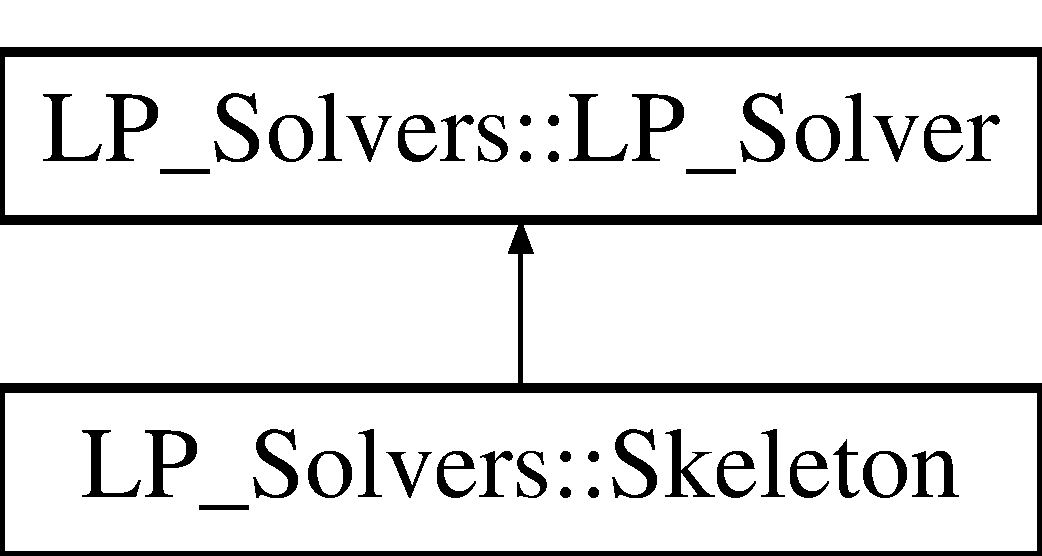
\includegraphics[height=2.000000cm]{group___c_l_s_solvers}
\end{center}
\end{figure}
\subsubsection*{Public Member Functions}
\begin{Indent}\textbf{ Construction}\par
\begin{DoxyCompactItemize}
\item 
\mbox{\Hypertarget{group___c_l_s_solvers_aa63d9454338c84be898e1a604eba3527}\label{group___c_l_s_solvers_aa63d9454338c84be898e1a604eba3527}} 
void \hyperlink{group___c_l_s_solvers_aa63d9454338c84be898e1a604eba3527}{common\+\_\+initialization} (N\+V\+A\+R\+\_\+\+T\+Y\+PE)
\begin{DoxyCompactList}\small\item\em Initialization common to all constructors. \end{DoxyCompactList}\item 
\hyperlink{group___c_l_s_solvers_ad9f2f64c49dbf96ebd30852e670e7642}{Skeleton} (N\+V\+A\+R\+\_\+\+T\+Y\+PE)
\begin{DoxyCompactList}\small\item\em Constructs a basic skeleton in the given number of dimensions, initialized to the axes, or (equivalently) to the set of constraints $ x_i \geq 0 $. \end{DoxyCompactList}\item 
\hyperlink{group___c_l_s_solvers_ad61d70c2397e93141de3ad3c987b1828}{Skeleton} (N\+V\+A\+R\+\_\+\+T\+Y\+PE, const vector$<$ \hyperlink{group___c_l_s_solvers_class_l_p___solvers_1_1_constraint}{Constraint} $>$ \&)
\begin{DoxyCompactList}\small\item\em Constructs a skeleton described by the given system of constraints. \end{DoxyCompactList}\item 
\mbox{\Hypertarget{group___c_l_s_solvers_ae1d6983329c8624014fa5c9d66f75ac3}\label{group___c_l_s_solvers_ae1d6983329c8624014fa5c9d66f75ac3}} 
\hyperlink{group___c_l_s_solvers_ae1d6983329c8624014fa5c9d66f75ac3}{Skeleton} (\hyperlink{group___c_l_s_solvers_class_l_p___solvers_1_1_skeleton}{Skeleton} \&)
\begin{DoxyCompactList}\small\item\em Performs a deep copy of {\ttfamily other}. \end{DoxyCompactList}\item 
virtual bool \hyperlink{group___c_l_s_solvers_a33b1747069c512ad69e30cb0c8786577}{copy} (const \hyperlink{group___c_l_s_solvers_class_l_p___solvers_1_1_l_p___solver}{L\+P\+\_\+\+Solver} $\ast$)
\begin{DoxyCompactList}\small\item\em performs a deep copy, similar to a copy constructor \end{DoxyCompactList}\end{DoxyCompactItemize}
\end{Indent}
\begin{Indent}\textbf{ Destruction}\par
\begin{DoxyCompactItemize}
\item 
\mbox{\Hypertarget{group___c_l_s_solvers_a0da8ede73aea9089d7b81683c08cfc60}\label{group___c_l_s_solvers_a0da8ede73aea9089d7b81683c08cfc60}} 
virtual \hyperlink{group___c_l_s_solvers_a0da8ede73aea9089d7b81683c08cfc60}{$\sim$\+Skeleton} ()
\begin{DoxyCompactList}\small\item\em Currently does nothing the compiler wouldn\textquotesingle{}t do. \end{DoxyCompactList}\end{DoxyCompactItemize}
\end{Indent}
\begin{Indent}\textbf{ Basic properties}\par
\begin{DoxyCompactItemize}
\item 
\mbox{\Hypertarget{group___c_l_s_solvers_acc02076b2e475b60d31104e15d4c982c}\label{group___c_l_s_solvers_acc02076b2e475b60d31104e15d4c982c}} 
N\+V\+A\+R\+\_\+\+T\+Y\+PE \hyperlink{group___c_l_s_solvers_acc02076b2e475b60d31104e15d4c982c}{get\+\_\+dimension} () const
\begin{DoxyCompactList}\small\item\em Returns the dimension of the underlying vector space. \end{DoxyCompactList}\item 
\mbox{\Hypertarget{group___c_l_s_solvers_a310919f8faa248ffa479004d91c4defa}\label{group___c_l_s_solvers_a310919f8faa248ffa479004d91c4defa}} 
unsigned long \hyperlink{group___c_l_s_solvers_a310919f8faa248ffa479004d91c4defa}{get\+\_\+number\+\_\+of\+\_\+edges} ()
\begin{DoxyCompactList}\small\item\em Returns the number of edges defining the skeleton. \end{DoxyCompactList}\item 
\mbox{\Hypertarget{group___c_l_s_solvers_aac51e256cb56e7fe4844c206dcfcf35b}\label{group___c_l_s_solvers_aac51e256cb56e7fe4844c206dcfcf35b}} 
set$<$ \hyperlink{group___c_l_s_solvers_class_l_p___solvers_1_1_edge}{Edge} $>$ \hyperlink{group___c_l_s_solvers_aac51e256cb56e7fe4844c206dcfcf35b}{get\+\_\+edges} ()
\begin{DoxyCompactList}\small\item\em Returns the edges that define the skeleton. \end{DoxyCompactList}\item 
\mbox{\Hypertarget{group___c_l_s_solvers_a1fcb6873ce96085aa68f97064cd90c9d}\label{group___c_l_s_solvers_a1fcb6873ce96085aa68f97064cd90c9d}} 
unsigned long \hyperlink{group___c_l_s_solvers_a1fcb6873ce96085aa68f97064cd90c9d}{get\+\_\+number\+\_\+of\+\_\+constraints} ()
\begin{DoxyCompactList}\small\item\em Returns the number of constraints defining the skeleton. \end{DoxyCompactList}\item 
\mbox{\Hypertarget{group___c_l_s_solvers_a7e1d8c1c056b9ec770f0c9abacdabe5d}\label{group___c_l_s_solvers_a7e1d8c1c056b9ec770f0c9abacdabe5d}} 
const vector$<$ \hyperlink{group___c_l_s_solvers_class_l_p___solvers_1_1_constraint}{Constraint} $>$ \& \hyperlink{group___c_l_s_solvers_a7e1d8c1c056b9ec770f0c9abacdabe5d}{get\+\_\+constraints} ()
\begin{DoxyCompactList}\small\item\em Returns the constraints that define the skeleton. \end{DoxyCompactList}\item 
\mbox{\Hypertarget{group___c_l_s_solvers_abbc8543d03ed7464149e6dba20f77da1}\label{group___c_l_s_solvers_abbc8543d03ed7464149e6dba20f77da1}} 
const \hyperlink{group___c_l_s_solvers_class_l_p___solvers_1_1_constraint}{Constraint} \& \hyperlink{group___c_l_s_solvers_abbc8543d03ed7464149e6dba20f77da1}{get\+\_\+constraint} (int index)
\begin{DoxyCompactList}\small\item\em Returns the indicated constraint. Numbering starts at 0. \end{DoxyCompactList}\end{DoxyCompactItemize}
\end{Indent}
\begin{Indent}\textbf{ Computation}\par
\begin{DoxyCompactItemize}
\item 
\mbox{\Hypertarget{group___c_l_s_solvers_ac6e9aadc18f4f7e0d3860682cae3bdf7}\label{group___c_l_s_solvers_ac6e9aadc18f4f7e0d3860682cae3bdf7}} 
void \hyperlink{group___c_l_s_solvers_ac6e9aadc18f4f7e0d3860682cae3bdf7}{which\+\_\+constraints\+\_\+active\+\_\+at} (const \hyperlink{group___c_l_s_solvers_class_l_p___solvers_1_1_ray}{Ray} \&u, bool $\ast$result) const
\begin{DoxyCompactList}\small\item\em returns the set of constraints in the skeleton active at {\ttfamily u} \end{DoxyCompactList}\item 
\mbox{\Hypertarget{group___c_l_s_solvers_a97d4c6e4864a90140728d664c8de12cf}\label{group___c_l_s_solvers_a97d4c6e4864a90140728d664c8de12cf}} 
bool \hyperlink{group___c_l_s_solvers_a97d4c6e4864a90140728d664c8de12cf}{is\+\_\+consistent} (const \hyperlink{group___c_l_s_solvers_class_l_p___solvers_1_1_constraint}{Constraint} \&c) const
\begin{DoxyCompactList}\small\item\em tests for consistency of a potentially new constraint. \end{DoxyCompactList}\end{DoxyCompactItemize}
\end{Indent}
\begin{Indent}\textbf{ Modification}\par
\begin{DoxyCompactItemize}
\item 
virtual bool \hyperlink{group___c_l_s_solvers_aba082a338a2cb3ace612fd2dfba667c5}{solve} (const vector$<$ \hyperlink{group___c_l_s_solvers_class_l_p___solvers_1_1_constraint}{Constraint} $>$ \&)
\begin{DoxyCompactList}\small\item\em Adds the indicated constraints (plural!) and re-\/computes the skeleton. \end{DoxyCompactList}\item 
virtual bool \hyperlink{group___c_l_s_solvers_a202b0b37e0ea8a817ce6e29c93a39cd8}{solve} (const \hyperlink{group___c_l_s_solvers_class_l_p___solvers_1_1_constraint}{Constraint} \&)
\begin{DoxyCompactList}\small\item\em Adds the indicated constraint (singular!) and re-\/computes the skeleton. \end{DoxyCompactList}\item 
\mbox{\Hypertarget{group___c_l_s_solvers_a91e67ca8a8fc7a891534462c21051ea1}\label{group___c_l_s_solvers_a91e67ca8a8fc7a891534462c21051ea1}} 
set$<$ \hyperlink{group___c_l_s_solvers_class_l_p___solvers_1_1_edge}{Edge} $>$ \hyperlink{group___c_l_s_solvers_a91e67ca8a8fc7a891534462c21051ea1}{adjacencies\+\_\+by\+\_\+graphs} (const set$<$ \hyperlink{group___c_l_s_solvers_class_l_p___solvers_1_1_ray}{Ray} $>$ \&)
\begin{DoxyCompactList}\small\item\em Re-\/computes the edges in the skeleton using Zolotych\textquotesingle{}s {\ttfamily Graph\+Adj} algorithm and returns the result. \end{DoxyCompactList}\item 
\mbox{\Hypertarget{group___c_l_s_solvers_a6ca243248975b2f1935169d78c44033b}\label{group___c_l_s_solvers_a6ca243248975b2f1935169d78c44033b}} 
\hyperlink{group___c_l_s_solvers_class_l_p___solvers_1_1_skeleton}{Skeleton} \& \hyperlink{group___c_l_s_solvers_a6ca243248975b2f1935169d78c44033b}{operator=} (const \hyperlink{group___c_l_s_solvers_class_l_p___solvers_1_1_skeleton}{Skeleton} \&)
\begin{DoxyCompactList}\small\item\em Assignment operator; empties current set \& copies from other. \end{DoxyCompactList}\end{DoxyCompactItemize}
\end{Indent}
\subsubsection*{Friends}
\begin{Indent}\textbf{ I/O}\par
\begin{DoxyCompactItemize}
\item 
ostream \& \hyperlink{group___c_l_s_solvers_a54f8dc187ec3e238ccc80d7a44b9ca82}{operator$<$$<$} (ostream \&os, const \hyperlink{group___c_l_s_solvers_class_l_p___solvers_1_1_skeleton}{Skeleton} \&s)
\begin{DoxyCompactList}\small\item\em prints out the constraints, then the rays, then the edges of {\ttfamily s}. \end{DoxyCompactList}\end{DoxyCompactItemize}
\end{Indent}
\subsection*{Additional Inherited Members}


\paragraph{Constructor \& Destructor Documentation}
\mbox{\Hypertarget{group___c_l_s_solvers_ad9f2f64c49dbf96ebd30852e670e7642}\label{group___c_l_s_solvers_ad9f2f64c49dbf96ebd30852e670e7642}} 
\index{L\+P\+\_\+\+Solvers\+::\+Skeleton@{L\+P\+\_\+\+Solvers\+::\+Skeleton}!Skeleton@{Skeleton}}
\index{Skeleton@{Skeleton}!L\+P\+\_\+\+Solvers\+::\+Skeleton@{L\+P\+\_\+\+Solvers\+::\+Skeleton}}
\subparagraph{\texorpdfstring{Skeleton()}{Skeleton()}\hspace{0.1cm}{\footnotesize\ttfamily [1/2]}}
{\footnotesize\ttfamily L\+P\+\_\+\+Solvers\+::\+Skeleton\+::\+Skeleton (\begin{DoxyParamCaption}\item[{N\+V\+A\+R\+\_\+\+T\+Y\+PE}]{dimension }\end{DoxyParamCaption})}



Constructs a basic skeleton in the given number of dimensions, initialized to the axes, or (equivalently) to the set of constraints $ x_i \geq 0 $. 

The rays are informed of their active constraints. \begin{DoxyPrecond}{Precondition}
the argument should be at least two 
\end{DoxyPrecond}
\begin{DoxyPostcond}{Postcondition}
the skeleton of the positive orthant 
\end{DoxyPostcond}


Definition at line 124 of file skeleton.\+cpp.

\mbox{\Hypertarget{group___c_l_s_solvers_ad61d70c2397e93141de3ad3c987b1828}\label{group___c_l_s_solvers_ad61d70c2397e93141de3ad3c987b1828}} 
\index{L\+P\+\_\+\+Solvers\+::\+Skeleton@{L\+P\+\_\+\+Solvers\+::\+Skeleton}!Skeleton@{Skeleton}}
\index{Skeleton@{Skeleton}!L\+P\+\_\+\+Solvers\+::\+Skeleton@{L\+P\+\_\+\+Solvers\+::\+Skeleton}}
\subparagraph{\texorpdfstring{Skeleton()}{Skeleton()}\hspace{0.1cm}{\footnotesize\ttfamily [2/2]}}
{\footnotesize\ttfamily L\+P\+\_\+\+Solvers\+::\+Skeleton\+::\+Skeleton (\begin{DoxyParamCaption}\item[{N\+V\+A\+R\+\_\+\+T\+Y\+PE}]{dimension,  }\item[{const vector$<$ \hyperlink{group___c_l_s_solvers_class_l_p___solvers_1_1_constraint}{Constraint} $>$ \&}]{constraints }\end{DoxyParamCaption})}



Constructs a skeleton described by the given system of constraints. 

Practically speaking, it first generates a basic skeleton, then iterates on the given constraints. \begin{DoxyPrecond}{Precondition}
{\ttfamily u.\+size() == v.\+size()} for all {\ttfamily u}, {\ttfamily v} in the vector 
\end{DoxyPrecond}
\begin{DoxyPostcond}{Postcondition}
unless the system supplied was inconsistent, a valid skeleton of the corresponding polyhedral cone 
\end{DoxyPostcond}
\begin{DoxyWarning}{Warning}
Your program will almost certainly fail if you do not respect the precondition. 
\end{DoxyWarning}


Definition at line 129 of file skeleton.\+cpp.



\paragraph{Member Function Documentation}
\mbox{\Hypertarget{group___c_l_s_solvers_a33b1747069c512ad69e30cb0c8786577}\label{group___c_l_s_solvers_a33b1747069c512ad69e30cb0c8786577}} 
\index{L\+P\+\_\+\+Solvers\+::\+Skeleton@{L\+P\+\_\+\+Solvers\+::\+Skeleton}!copy@{copy}}
\index{copy@{copy}!L\+P\+\_\+\+Solvers\+::\+Skeleton@{L\+P\+\_\+\+Solvers\+::\+Skeleton}}
\subparagraph{\texorpdfstring{copy()}{copy()}}
{\footnotesize\ttfamily bool L\+P\+\_\+\+Solvers\+::\+Skeleton\+::copy (\begin{DoxyParamCaption}\item[{const \hyperlink{group___c_l_s_solvers_class_l_p___solvers_1_1_l_p___solver}{L\+P\+\_\+\+Solver} $\ast$}]{ }\end{DoxyParamCaption})\hspace{0.3cm}{\ttfamily [virtual]}}



performs a deep copy, similar to a copy constructor 

\begin{DoxyReturn}{Returns}
{\ttfamily true} iff copying was successful 
\end{DoxyReturn}
\begin{DoxyWarning}{Warning}
Do not mix-\/and-\/match solvers. At the present time, a \hyperlink{group___c_l_s_solvers_class_l_p___solvers_1_1_p_p_l___solver}{P\+P\+L\+\_\+\+Solver} is not equipped to copy a \hyperlink{group___c_l_s_solvers_class_l_p___solvers_1_1_g_l_p_k___solver}{G\+L\+P\+K\+\_\+\+Solver}, or vice versa. (This doesn\textquotesingle{}t even make sense between exact and approximate solvers.) 
\end{DoxyWarning}


Implements \hyperlink{group___c_l_s_solvers_a36c14a88e9d3ae9d9321acc7877236d0}{L\+P\+\_\+\+Solvers\+::\+L\+P\+\_\+\+Solver}.



Definition at line 145 of file skeleton.\+cpp.

\mbox{\Hypertarget{group___c_l_s_solvers_aba082a338a2cb3ace612fd2dfba667c5}\label{group___c_l_s_solvers_aba082a338a2cb3ace612fd2dfba667c5}} 
\index{L\+P\+\_\+\+Solvers\+::\+Skeleton@{L\+P\+\_\+\+Solvers\+::\+Skeleton}!solve@{solve}}
\index{solve@{solve}!L\+P\+\_\+\+Solvers\+::\+Skeleton@{L\+P\+\_\+\+Solvers\+::\+Skeleton}}
\subparagraph{\texorpdfstring{solve()}{solve()}\hspace{0.1cm}{\footnotesize\ttfamily [1/2]}}
{\footnotesize\ttfamily bool L\+P\+\_\+\+Solvers\+::\+Skeleton\+::solve (\begin{DoxyParamCaption}\item[{const vector$<$ \hyperlink{group___c_l_s_solvers_class_l_p___solvers_1_1_constraint}{Constraint} $>$ \&}]{new\+\_\+constraints }\end{DoxyParamCaption})\hspace{0.3cm}{\ttfamily [virtual]}}



Adds the indicated constraints (plural!) and re-\/computes the skeleton. 

\begin{DoxyReturn}{Returns}
{\ttfamily true} if and only if the new constraints are consistent with the current constraints
\end{DoxyReturn}
\begin{DoxyWarning}{Warning}
Checking the return value is crucial! If the function returns {\ttfamily false}, you have an inconsistent system! While the {\itshape present} cone will remain consistent, {\bfseries the function will not roll back previous changes you have made}, so if you want to iterate again, your best bet is to copy the skeleton, and try that copy. Accept the new constraints only if that copy succeeds, in which case, you might as well discard the original, and keep the copy. 
\end{DoxyWarning}


Implements \hyperlink{group___c_l_s_solvers_aea1a5bf98a2c4c06b0550cacdf8b88fd}{L\+P\+\_\+\+Solvers\+::\+L\+P\+\_\+\+Solver}.



Definition at line 275 of file skeleton.\+cpp.

\mbox{\Hypertarget{group___c_l_s_solvers_a202b0b37e0ea8a817ce6e29c93a39cd8}\label{group___c_l_s_solvers_a202b0b37e0ea8a817ce6e29c93a39cd8}} 
\index{L\+P\+\_\+\+Solvers\+::\+Skeleton@{L\+P\+\_\+\+Solvers\+::\+Skeleton}!solve@{solve}}
\index{solve@{solve}!L\+P\+\_\+\+Solvers\+::\+Skeleton@{L\+P\+\_\+\+Solvers\+::\+Skeleton}}
\subparagraph{\texorpdfstring{solve()}{solve()}\hspace{0.1cm}{\footnotesize\ttfamily [2/2]}}
{\footnotesize\ttfamily bool L\+P\+\_\+\+Solvers\+::\+Skeleton\+::solve (\begin{DoxyParamCaption}\item[{const \hyperlink{group___c_l_s_solvers_class_l_p___solvers_1_1_constraint}{Constraint} \&}]{constraint }\end{DoxyParamCaption})\hspace{0.3cm}{\ttfamily [virtual]}}



Adds the indicated constraint (singular!) and re-\/computes the skeleton. 

\begin{DoxyReturn}{Returns}
{\ttfamily true} if and only if the new constraint is consistent with the current constraints
\end{DoxyReturn}
\begin{DoxyWarning}{Warning}
Checking the return value is crucial! If the function returns {\ttfamily false}, you have an inconsistent system! While the {\itshape present} cone will remain consistent, {\bfseries the function will not roll back previous changes you have made}, so if you want to iterate again, your best bet is to copy the skeleton, and try that copy. Accept the new constraints only if that copy succeeds, in which case, you might as well discard the original, and keep the copy. 
\end{DoxyWarning}


Implements \hyperlink{group___c_l_s_solvers_a8b9979fb228ac9ccfe037ad6ca48b314}{L\+P\+\_\+\+Solvers\+::\+L\+P\+\_\+\+Solver}.



Definition at line 167 of file skeleton.\+cpp.



\paragraph{Friends And Related Function Documentation}
\mbox{\Hypertarget{group___c_l_s_solvers_a54f8dc187ec3e238ccc80d7a44b9ca82}\label{group___c_l_s_solvers_a54f8dc187ec3e238ccc80d7a44b9ca82}} 
\index{L\+P\+\_\+\+Solvers\+::\+Skeleton@{L\+P\+\_\+\+Solvers\+::\+Skeleton}!operator$<$$<$@{operator$<$$<$}}
\index{operator$<$$<$@{operator$<$$<$}!L\+P\+\_\+\+Solvers\+::\+Skeleton@{L\+P\+\_\+\+Solvers\+::\+Skeleton}}
\subparagraph{\texorpdfstring{operator$<$$<$}{operator<<}}
{\footnotesize\ttfamily ostream\& operator$<$$<$ (\begin{DoxyParamCaption}\item[{ostream \&}]{os,  }\item[{const \hyperlink{group___c_l_s_solvers_class_l_p___solvers_1_1_skeleton}{Skeleton} \&}]{s }\end{DoxyParamCaption})\hspace{0.3cm}{\ttfamily [friend]}}



prints out the constraints, then the rays, then the edges of {\ttfamily s}. 


\begin{DoxyParams}{Parameters}
{\em os} & output stream to print to \\
\hline
{\em s} & skeleton to print \\
\hline
\end{DoxyParams}
\begin{DoxyReturn}{Returns}
the output stream 
\end{DoxyReturn}


Definition at line 440 of file skeleton.\+cpp.



\subsection{Function Documentation}
\mbox{\Hypertarget{group___c_l_s_solvers_gaf3434d5c281c16ef7a09d8f73445ea00}\label{group___c_l_s_solvers_gaf3434d5c281c16ef7a09d8f73445ea00}} 
\index{Constrained Linear System Solvers@{Constrained Linear System Solvers}!intersections\+\_\+of\+\_\+active\+\_\+constraints@{intersections\+\_\+of\+\_\+active\+\_\+constraints}}
\index{intersections\+\_\+of\+\_\+active\+\_\+constraints@{intersections\+\_\+of\+\_\+active\+\_\+constraints}!Constrained Linear System Solvers@{Constrained Linear System Solvers}}
\subsubsection{\texorpdfstring{intersections\+\_\+of\+\_\+active\+\_\+constraints()}{intersections\_of\_active\_constraints()}\hspace{0.1cm}{\footnotesize\ttfamily [1/2]}}
{\footnotesize\ttfamily vector$<$bool$>$ L\+P\+\_\+\+Solvers\+::intersections\+\_\+of\+\_\+active\+\_\+constraints (\begin{DoxyParamCaption}\item[{bool $\ast$}]{,  }\item[{bool $\ast$}]{,  }\item[{unsigned}]{ }\end{DoxyParamCaption})}



indicates which constraints are active for both sets 

\begin{DoxyReturn}{Returns}
the intersection between the given sets of constraints. 
\end{DoxyReturn}
\mbox{\Hypertarget{group___c_l_s_solvers_ga1f87ac127ced7d681b3e51e38eef0cf4}\label{group___c_l_s_solvers_ga1f87ac127ced7d681b3e51e38eef0cf4}} 
\index{Constrained Linear System Solvers@{Constrained Linear System Solvers}!intersections\+\_\+of\+\_\+active\+\_\+constraints@{intersections\+\_\+of\+\_\+active\+\_\+constraints}}
\index{intersections\+\_\+of\+\_\+active\+\_\+constraints@{intersections\+\_\+of\+\_\+active\+\_\+constraints}!Constrained Linear System Solvers@{Constrained Linear System Solvers}}
\subsubsection{\texorpdfstring{intersections\+\_\+of\+\_\+active\+\_\+constraints()}{intersections\_of\_active\_constraints()}\hspace{0.1cm}{\footnotesize\ttfamily [2/2]}}
{\footnotesize\ttfamily void L\+P\+\_\+\+Solvers\+::intersections\+\_\+of\+\_\+active\+\_\+constraints (\begin{DoxyParamCaption}\item[{bool $\ast$}]{a,  }\item[{bool $\ast$}]{b,  }\item[{bool $\ast$}]{result,  }\item[{unsigned}]{m }\end{DoxyParamCaption})}



indicates which constraints are active for both sets 


\begin{DoxyParams}{Parameters}
{\em a} & first set \\
\hline
{\em b} & second set \\
\hline
{\em result} & set where {\ttfamily true} occurs only if it does in both {\ttfamily a} and {\ttfamily b} \\
\hline
{\em m} & number of entries in {\ttfamily a} and {\ttfamily b} \\
\hline
\end{DoxyParams}
\begin{DoxyReturn}{Returns}
the intersection between the given sets of constraints. 
\end{DoxyReturn}


Definition at line 321 of file skeleton.\+cpp.

\mbox{\Hypertarget{group___c_l_s_solvers_ga0a997634a9b11bec9c54d0243ac29008}\label{group___c_l_s_solvers_ga0a997634a9b11bec9c54d0243ac29008}} 
\index{Constrained Linear System Solvers@{Constrained Linear System Solvers}!is\+\_\+first\+\_\+subset\+\_\+of\+\_\+second@{is\+\_\+first\+\_\+subset\+\_\+of\+\_\+second}}
\index{is\+\_\+first\+\_\+subset\+\_\+of\+\_\+second@{is\+\_\+first\+\_\+subset\+\_\+of\+\_\+second}!Constrained Linear System Solvers@{Constrained Linear System Solvers}}
\subsubsection{\texorpdfstring{is\+\_\+first\+\_\+subset\+\_\+of\+\_\+second()}{is\_first\_subset\_of\_second()}}
{\footnotesize\ttfamily bool L\+P\+\_\+\+Solvers\+::is\+\_\+first\+\_\+subset\+\_\+of\+\_\+second (\begin{DoxyParamCaption}\item[{bool $\ast$}]{,  }\item[{bool $\ast$}]{,  }\item[{unsigned}]{ }\end{DoxyParamCaption})}



determines whether the first set of active constraints is a subset of the second 

\begin{DoxyReturn}{Returns}
{\ttfamily true} if and only if the first set is a subset of the second. 
\end{DoxyReturn}


Definition at line 335 of file skeleton.\+cpp.

\mbox{\Hypertarget{group___c_l_s_solvers_gad030de457424bef601e2903eb619926e}\label{group___c_l_s_solvers_gad030de457424bef601e2903eb619926e}} 
\index{Constrained Linear System Solvers@{Constrained Linear System Solvers}!number\+\_\+of\+\_\+common\+\_\+constraints@{number\+\_\+of\+\_\+common\+\_\+constraints}}
\index{number\+\_\+of\+\_\+common\+\_\+constraints@{number\+\_\+of\+\_\+common\+\_\+constraints}!Constrained Linear System Solvers@{Constrained Linear System Solvers}}
\subsubsection{\texorpdfstring{number\+\_\+of\+\_\+common\+\_\+constraints()}{number\_of\_common\_constraints()}}
{\footnotesize\ttfamily int L\+P\+\_\+\+Solvers\+::number\+\_\+of\+\_\+common\+\_\+constraints (\begin{DoxyParamCaption}\item[{bool $\ast$}]{,  }\item[{bool $\ast$}]{,  }\item[{unsigned}]{ }\end{DoxyParamCaption})}



counts the number of constraints active in both sets 

\begin{DoxyReturn}{Returns}
the number of constraints common to both sets. 
\end{DoxyReturn}


Definition at line 302 of file skeleton.\+cpp.

\mbox{\Hypertarget{group___c_l_s_solvers_gaf71a7e68f920518b02b6a58660594ca2}\label{group___c_l_s_solvers_gaf71a7e68f920518b02b6a58660594ca2}} 
\index{Constrained Linear System Solvers@{Constrained Linear System Solvers}!operator$\ast$@{operator$\ast$}}
\index{operator$\ast$@{operator$\ast$}!Constrained Linear System Solvers@{Constrained Linear System Solvers}}
\subsubsection{\texorpdfstring{operator$\ast$()}{operator*()}\hspace{0.1cm}{\footnotesize\ttfamily [1/6]}}
{\footnotesize\ttfamily \hyperlink{group___c_l_s_solvers_class_l_p___solvers_1_1_ray}{Ray} L\+P\+\_\+\+Solvers\+::operator$\ast$ (\begin{DoxyParamCaption}\item[{const R\+A\+Y\+E\+N\+T\+\_\+\+T\+Y\+PE}]{,  }\item[{const \hyperlink{group___c_l_s_solvers_class_l_p___solvers_1_1_ray}{Ray} \&}]{ }\end{DoxyParamCaption})}



Multiply every coordinate in the given ray by the given scalar. 

\begin{DoxyReturn}{Returns}
a copy of the ray, scaled by the requesed amount 
\end{DoxyReturn}


Definition at line 224 of file lp\+\_\+solver.\+cpp.

\mbox{\Hypertarget{group___c_l_s_solvers_gaae1f5d07b6d0f4c12b4c7835977b64eb}\label{group___c_l_s_solvers_gaae1f5d07b6d0f4c12b4c7835977b64eb}} 
\index{Constrained Linear System Solvers@{Constrained Linear System Solvers}!operator$\ast$@{operator$\ast$}}
\index{operator$\ast$@{operator$\ast$}!Constrained Linear System Solvers@{Constrained Linear System Solvers}}
\subsubsection{\texorpdfstring{operator$\ast$()}{operator*()}\hspace{0.1cm}{\footnotesize\ttfamily [2/6]}}
{\footnotesize\ttfamily R\+A\+Y\+E\+N\+T\+\_\+\+T\+Y\+PE L\+P\+\_\+\+Solvers\+::operator$\ast$ (\begin{DoxyParamCaption}\item[{const \hyperlink{group___c_l_s_solvers_class_l_p___solvers_1_1_ray}{Ray} \&}]{,  }\item[{const \hyperlink{group___c_l_s_solvers_class_l_p___solvers_1_1_ray}{Ray} \&}]{ }\end{DoxyParamCaption})}



Compute the dot product on the rays. 

\begin{DoxyReturn}{Returns}
the dot product of the rays 
\end{DoxyReturn}
\begin{DoxyWarning}{Warning}
This is unsafe when dimension is not the same. It does not check, since the assumption is that you know what you\textquotesingle{}re doing. 
\end{DoxyWarning}


Definition at line 237 of file lp\+\_\+solver.\+cpp.

\mbox{\Hypertarget{group___c_l_s_solvers_ga9b4f6991b325c2a42e1f14fc09346277}\label{group___c_l_s_solvers_ga9b4f6991b325c2a42e1f14fc09346277}} 
\index{Constrained Linear System Solvers@{Constrained Linear System Solvers}!operator$\ast$@{operator$\ast$}}
\index{operator$\ast$@{operator$\ast$}!Constrained Linear System Solvers@{Constrained Linear System Solvers}}
\subsubsection{\texorpdfstring{operator$\ast$()}{operator*()}\hspace{0.1cm}{\footnotesize\ttfamily [3/6]}}
{\footnotesize\ttfamily R\+A\+Y\+E\+N\+T\+\_\+\+T\+Y\+PE L\+P\+\_\+\+Solvers\+::operator$\ast$ (\begin{DoxyParamCaption}\item[{const \hyperlink{group___c_l_s_solvers_class_l_p___solvers_1_1_ray}{Ray} \&}]{,  }\item[{const vector$<$ long $>$ \&}]{ }\end{DoxyParamCaption})}



compute the dot product of the specified rays, one of which is a vector 

\begin{DoxyReturn}{Returns}
the dot product 
\end{DoxyReturn}
\begin{DoxyWarning}{Warning}
This is unsafe when dimension is not the same. It does not check, since the assumption is that you know what you\textquotesingle{}re doing. 
\end{DoxyWarning}


Definition at line 245 of file lp\+\_\+solver.\+cpp.

\mbox{\Hypertarget{group___c_l_s_solvers_gab64c33abcc54e5b175b7b567e099c75b}\label{group___c_l_s_solvers_gab64c33abcc54e5b175b7b567e099c75b}} 
\index{Constrained Linear System Solvers@{Constrained Linear System Solvers}!operator$\ast$@{operator$\ast$}}
\index{operator$\ast$@{operator$\ast$}!Constrained Linear System Solvers@{Constrained Linear System Solvers}}
\subsubsection{\texorpdfstring{operator$\ast$()}{operator*()}\hspace{0.1cm}{\footnotesize\ttfamily [4/6]}}
{\footnotesize\ttfamily R\+A\+Y\+E\+N\+T\+\_\+\+T\+Y\+PE L\+P\+\_\+\+Solvers\+::operator$\ast$ (\begin{DoxyParamCaption}\item[{const vector$<$ long $>$ \&}]{,  }\item[{const \hyperlink{group___c_l_s_solvers_class_l_p___solvers_1_1_ray}{Ray} \&}]{ }\end{DoxyParamCaption})}



compute the dot product of the specified rays, one of which is a vector 

\begin{DoxyReturn}{Returns}
the dot product 
\end{DoxyReturn}
\begin{DoxyWarning}{Warning}
This is unsafe when dimension is not the same. It does not check, since the assumption is that you know what you\textquotesingle{}re doing. 
\end{DoxyWarning}


Definition at line 253 of file lp\+\_\+solver.\+cpp.

\mbox{\Hypertarget{group___c_l_s_solvers_gaea75db1559315f35242d62e9e5f66e92}\label{group___c_l_s_solvers_gaea75db1559315f35242d62e9e5f66e92}} 
\index{Constrained Linear System Solvers@{Constrained Linear System Solvers}!operator$\ast$@{operator$\ast$}}
\index{operator$\ast$@{operator$\ast$}!Constrained Linear System Solvers@{Constrained Linear System Solvers}}
\subsubsection{\texorpdfstring{operator$\ast$()}{operator*()}\hspace{0.1cm}{\footnotesize\ttfamily [5/6]}}
{\footnotesize\ttfamily D\+O\+T\+P\+R\+O\+D\+\_\+\+T\+Y\+PE L\+P\+\_\+\+Solvers\+::operator$\ast$ (\begin{DoxyParamCaption}\item[{const \hyperlink{group___c_l_s_solvers_class_l_p___solvers_1_1_ray}{Ray} \&}]{r,  }\item[{const \hyperlink{group___c_l_s_solvers_class_l_p___solvers_1_1_constraint}{Constraint} \&}]{c }\end{DoxyParamCaption})\hspace{0.3cm}{\ttfamily [inline]}}



Compute the dot product between the ray and the constraint. 


\begin{DoxyParams}{Parameters}
{\em r} & a ray \\
\hline
{\em c} & a constraint \\
\hline
\end{DoxyParams}
\begin{DoxyReturn}{Returns}
the dot product of the ray and the constraint 
\end{DoxyReturn}
\begin{DoxyWarning}{Warning}
This is unsafe when dimension is not the same. It does not check, since the assumption is that you know what you\textquotesingle{}re doing. 
\end{DoxyWarning}


Definition at line 525 of file lp\+\_\+solver.\+hpp.

\mbox{\Hypertarget{group___c_l_s_solvers_gaf9f83e5d45bfc080fbffde26ebb93892}\label{group___c_l_s_solvers_gaf9f83e5d45bfc080fbffde26ebb93892}} 
\index{Constrained Linear System Solvers@{Constrained Linear System Solvers}!operator$\ast$@{operator$\ast$}}
\index{operator$\ast$@{operator$\ast$}!Constrained Linear System Solvers@{Constrained Linear System Solvers}}
\subsubsection{\texorpdfstring{operator$\ast$()}{operator*()}\hspace{0.1cm}{\footnotesize\ttfamily [6/6]}}
{\footnotesize\ttfamily D\+O\+T\+P\+R\+O\+D\+\_\+\+T\+Y\+PE L\+P\+\_\+\+Solvers\+::operator$\ast$ (\begin{DoxyParamCaption}\item[{\hyperlink{group___c_l_s_solvers_class_l_p___solvers_1_1_constraint}{Constraint} \&}]{c,  }\item[{\hyperlink{group___c_l_s_solvers_class_l_p___solvers_1_1_ray}{Ray} \&}]{r }\end{DoxyParamCaption})\hspace{0.3cm}{\ttfamily [inline]}}



Compute the dot product between the ray and the constraint. 


\begin{DoxyParams}{Parameters}
{\em c} & a \hyperlink{group___c_l_s_solvers_class_l_p___solvers_1_1_constraint}{Constraint} \\
\hline
{\em r} & a ray \\
\hline
\end{DoxyParams}
\begin{DoxyReturn}{Returns}
the dot product of the ray and the constraint 
\end{DoxyReturn}
\begin{DoxyWarning}{Warning}
This is unsafe when dimension is not the same. It does not check, since the assumption is that you know what you\textquotesingle{}re doing. 
\end{DoxyWarning}


Definition at line 537 of file lp\+\_\+solver.\+hpp.

\mbox{\Hypertarget{group___c_l_s_solvers_gaf293c6d803dc697897463525aa1d1d44}\label{group___c_l_s_solvers_gaf293c6d803dc697897463525aa1d1d44}} 
\index{Constrained Linear System Solvers@{Constrained Linear System Solvers}!operator+@{operator+}}
\index{operator+@{operator+}!Constrained Linear System Solvers@{Constrained Linear System Solvers}}
\subsubsection{\texorpdfstring{operator+()}{operator+()}}
{\footnotesize\ttfamily \hyperlink{group___c_l_s_solvers_class_l_p___solvers_1_1_ray}{Ray} L\+P\+\_\+\+Solvers\+::operator+ (\begin{DoxyParamCaption}\item[{const \hyperlink{group___c_l_s_solvers_class_l_p___solvers_1_1_ray}{Ray} \&}]{,  }\item[{const \hyperlink{group___c_l_s_solvers_class_l_p___solvers_1_1_ray}{Ray} \&}]{ }\end{DoxyParamCaption})}



Add the two rays. 

\begin{DoxyReturn}{Returns}
the sum of the two rays 
\end{DoxyReturn}
\begin{DoxyWarning}{Warning}
This is unsafe when dimension is not the same. It does not check, since the assumption is that you know what you\textquotesingle{}re doing. 
\end{DoxyWarning}


Definition at line 261 of file lp\+\_\+solver.\+cpp.

\mbox{\Hypertarget{group___c_l_s_solvers_gac20f6443d37909c326bb31c0399ea634}\label{group___c_l_s_solvers_gac20f6443d37909c326bb31c0399ea634}} 
\index{Constrained Linear System Solvers@{Constrained Linear System Solvers}!operator-\/@{operator-\/}}
\index{operator-\/@{operator-\/}!Constrained Linear System Solvers@{Constrained Linear System Solvers}}
\subsubsection{\texorpdfstring{operator-\/()}{operator-()}}
{\footnotesize\ttfamily \hyperlink{group___c_l_s_solvers_class_l_p___solvers_1_1_ray}{Ray} L\+P\+\_\+\+Solvers\+::operator-\/ (\begin{DoxyParamCaption}\item[{const \hyperlink{group___c_l_s_solvers_class_l_p___solvers_1_1_ray}{Ray} \&}]{,  }\item[{const \hyperlink{group___c_l_s_solvers_class_l_p___solvers_1_1_ray}{Ray} \&}]{ }\end{DoxyParamCaption})}



Subtract the two rays. 

\begin{DoxyReturn}{Returns}
the difference of the two rays 
\end{DoxyReturn}
\begin{DoxyWarning}{Warning}
This is unsafe when dimension is not the same. It does not check, since the assumption is that you know what you\textquotesingle{}re doing. 
\end{DoxyWarning}


Definition at line 272 of file lp\+\_\+solver.\+cpp.

\mbox{\Hypertarget{group___c_l_s_solvers_ga42f6aa14b6c3adb4df26f8338d486401}\label{group___c_l_s_solvers_ga42f6aa14b6c3adb4df26f8338d486401}} 
\index{Constrained Linear System Solvers@{Constrained Linear System Solvers}!ray\+\_\+sum@{ray\+\_\+sum}}
\index{ray\+\_\+sum@{ray\+\_\+sum}!Constrained Linear System Solvers@{Constrained Linear System Solvers}}
\subsubsection{\texorpdfstring{ray\+\_\+sum()}{ray\_sum()}}
{\footnotesize\ttfamily \hyperlink{group___c_l_s_solvers_class_l_p___solvers_1_1_ray}{Ray} L\+P\+\_\+\+Solvers\+::ray\+\_\+sum (\begin{DoxyParamCaption}\item[{const set$<$ \hyperlink{group___c_l_s_solvers_class_l_p___solvers_1_1_ray}{Ray} $>$ \&}]{ }\end{DoxyParamCaption})}



Add all the rays in a set. 

\begin{DoxyReturn}{Returns}
a ray that is the sum of all rays in the given set 
\end{DoxyReturn}
\begin{DoxyWarning}{Warning}
This is unsafe when dimension is not the same. It does not check, since the assumption is that you know what you\textquotesingle{}re doing. 
\end{DoxyWarning}


Definition at line 283 of file lp\+\_\+solver.\+cpp.

\mbox{\Hypertarget{group___c_l_s_solvers_ga8b57096f9dac0f00912dd248cfdc89db}\label{group___c_l_s_solvers_ga8b57096f9dac0f00912dd248cfdc89db}} 
\index{Constrained Linear System Solvers@{Constrained Linear System Solvers}!union\+\_\+of\+\_\+edge\+\_\+sets@{union\+\_\+of\+\_\+edge\+\_\+sets}}
\index{union\+\_\+of\+\_\+edge\+\_\+sets@{union\+\_\+of\+\_\+edge\+\_\+sets}!Constrained Linear System Solvers@{Constrained Linear System Solvers}}
\subsubsection{\texorpdfstring{union\+\_\+of\+\_\+edge\+\_\+sets()}{union\_of\_edge\_sets()}}
{\footnotesize\ttfamily set$<$ \hyperlink{group___c_l_s_solvers_class_l_p___solvers_1_1_edge}{Edge} $>$ L\+P\+\_\+\+Solvers\+::union\+\_\+of\+\_\+edge\+\_\+sets (\begin{DoxyParamCaption}\item[{const set$<$ \hyperlink{group___c_l_s_solvers_class_l_p___solvers_1_1_edge}{Edge} $>$ \&}]{,  }\item[{const set$<$ \hyperlink{group___c_l_s_solvers_class_l_p___solvers_1_1_edge}{Edge} $>$ \&}]{ }\end{DoxyParamCaption})}



computes the union of the specified edge sets 

\begin{DoxyReturn}{Returns}
union of the specified edge sets 
\end{DoxyReturn}


Definition at line 347 of file skeleton.\+cpp.


\hypertarget{group___fields_group}{}\section{Fields}
\label{group___fields_group}\index{Fields@{Fields}}


classes for performing field arithmetic  


\subsection*{Classes}
\begin{DoxyCompactItemize}
\item 
class \hyperlink{group___fields_group_class_prime___field}{Prime\+\_\+\+Field}
\begin{DoxyCompactList}\small\item\em Information necessary for a field modulo a prime.  \hyperlink{group___fields_group_class_prime___field}{More...}\end{DoxyCompactList}\item 
class \hyperlink{group___fields_group_class_prime___field___element}{Prime\+\_\+\+Field\+\_\+\+Element}
\begin{DoxyCompactList}\small\item\em Element of a field of prime characteristic.  \hyperlink{group___fields_group_class_prime___field___element}{More...}\end{DoxyCompactList}\end{DoxyCompactItemize}


\subsection{Detailed Description}
classes for performing field arithmetic 



\subsection{Class Documentation}
\index{Prime\+\_\+\+Field@{Prime\+\_\+\+Field}}\label{class_prime___field}
\Hypertarget{group___fields_group_class_prime___field}
\subsubsection{class Prime\+\_\+\+Field}
Information necessary for a field modulo a prime. 

\begin{DoxyAuthor}{Author}
John Perry 
\end{DoxyAuthor}
\begin{DoxyDate}{Date}
2015
\end{DoxyDate}
This class encapsulates the information necessary for a field modulo a prime\+: both the modulus $m$ and a list of inverses of non-\/zero elements. The constructors do not verify that $m$ is prime, but expect misbehavior if not.

\begin{DoxyWarning}{Warning}
The constructor does not check whether the supplied modulus is prime. If $m$ is not prime, behavior is undefined, and probably spectacularly bad. 
\end{DoxyWarning}
\begin{Desc}
\item[Examples\+: ]\par
\hyperlink{test_4by4_8cpp-example}{test\+\_\+4by4.\+cpp}, \hyperlink{test_cab_es1_8cpp-example}{test\+\_\+cab\+\_\+es1.\+cpp}, \hyperlink{test_cab_es2_8cpp-example}{test\+\_\+cab\+\_\+es2.\+cpp}, \hyperlink{test_cab_es4_8cpp-example}{test\+\_\+cab\+\_\+es4.\+cpp}, \hyperlink{test_cab_es5_8cpp-example}{test\+\_\+cab\+\_\+es5.\+cpp}, \hyperlink{test_cab_es6_8cpp-example}{test\+\_\+cab\+\_\+es6.\+cpp}, \hyperlink{test_cab_es9_8cpp-example}{test\+\_\+cab\+\_\+es9.\+cpp}, \hyperlink{test_cyclic4_8cpp-example}{test\+\_\+cyclic4.\+cpp}, \hyperlink{test_cyclicn_8cpp-example}{test\+\_\+cyclicn.\+cpp}, \hyperlink{test_dynamic_8cpp-example}{test\+\_\+dynamic.\+cpp}, \hyperlink{test_monomials_8cpp-example}{test\+\_\+monomials.\+cpp}, and \hyperlink{user_interface_8cpp-example}{user\+\_\+interface.\+cpp}.\end{Desc}


Definition at line 51 of file fields.\+hpp.

\subsubsection*{Public Member Functions}
\begin{Indent}\textbf{ Construction}\par
\begin{DoxyCompactItemize}
\item 
\hyperlink{group___fields_group_a2a127ad161be0d732921c7a4bbd19779}{Prime\+\_\+\+Field} (U\+C\+O\+E\+F\+\_\+\+T\+Y\+PE \hyperlink{group___fields_group_a342ee34fa19d33919f772669a637f31e}{modulus}, bool show\+\_\+modulus=false)
\begin{DoxyCompactList}\small\item\em Please read detailed information. \end{DoxyCompactList}\item 
\hyperlink{group___fields_group_a99ac17cca00c87af9ca859c8eae11006}{Prime\+\_\+\+Field} (const \hyperlink{group___fields_group_class_prime___field}{Prime\+\_\+\+Field} \&F)
\begin{DoxyCompactList}\small\item\em Copy constructor\+: copies previously-\/computed inverses. \end{DoxyCompactList}\end{DoxyCompactItemize}
\end{Indent}
\begin{Indent}\textbf{ Destruction}\par
\begin{DoxyCompactItemize}
\item 
\mbox{\Hypertarget{group___fields_group_a0865fbb0bd4478219f64098ebb1e871d}\label{group___fields_group_a0865fbb0bd4478219f64098ebb1e871d}} 
{\bfseries $\sim$\+Prime\+\_\+\+Field} ()
\end{DoxyCompactItemize}
\end{Indent}
\begin{Indent}\textbf{ Basic properties}\par
{\em The following functions give information about the prime field, but do not modify it. }\begin{DoxyCompactItemize}
\item 
\mbox{\Hypertarget{group___fields_group_a342ee34fa19d33919f772669a637f31e}\label{group___fields_group_a342ee34fa19d33919f772669a637f31e}} 
unsigned \hyperlink{group___fields_group_a342ee34fa19d33919f772669a637f31e}{modulus} () const
\begin{DoxyCompactList}\small\item\em Returns the field\textquotesingle{}s modulus. \end{DoxyCompactList}\item 
C\+O\+E\+F\+\_\+\+T\+Y\+PE \hyperlink{group___fields_group_a106e74e004b18c899cd9b9e90ce01f6e}{inverse} (C\+O\+E\+F\+\_\+\+T\+Y\+PE a) const
\begin{DoxyCompactList}\small\item\em Returns the inverse of $a$, modulo $m$. \end{DoxyCompactList}\item 
\mbox{\Hypertarget{group___fields_group_a97534ab1050f0b34023300f1bd3a97f5}\label{group___fields_group_a97534ab1050f0b34023300f1bd3a97f5}} 
\hyperlink{group___fields_group_class_prime___field___element}{Prime\+\_\+\+Field\+\_\+\+Element} \hyperlink{group___fields_group_a97534ab1050f0b34023300f1bd3a97f5}{unity} () const
\begin{DoxyCompactList}\small\item\em ``unity'' is the multiplicative identity. \end{DoxyCompactList}\item 
\mbox{\Hypertarget{group___fields_group_ad8eaaf37b9239428a9c9aedc8ab35a12}\label{group___fields_group_ad8eaaf37b9239428a9c9aedc8ab35a12}} 
\hyperlink{group___fields_group_class_prime___field___element}{Prime\+\_\+\+Field\+\_\+\+Element} \hyperlink{group___fields_group_ad8eaaf37b9239428a9c9aedc8ab35a12}{zero} () const
\begin{DoxyCompactList}\small\item\em ``zero'' is the additive identity. \end{DoxyCompactList}\end{DoxyCompactItemize}
\end{Indent}
\begin{Indent}\textbf{ I/O}\par
\begin{DoxyCompactItemize}
\item 
\mbox{\Hypertarget{group___fields_group_a1ff3ec98ffb33a35c51eb3ce99ae7ebd}\label{group___fields_group_a1ff3ec98ffb33a35c51eb3ce99ae7ebd}} 
void \hyperlink{group___fields_group_a1ff3ec98ffb33a35c51eb3ce99ae7ebd}{set\+\_\+print\+\_\+modulus} (bool b)
\begin{DoxyCompactList}\small\item\em determines whether to print the modulus \end{DoxyCompactList}\item 
\mbox{\Hypertarget{group___fields_group_a5ac5cf31e741cc6d250176163bde658c}\label{group___fields_group_a5ac5cf31e741cc6d250176163bde658c}} 
bool \hyperlink{group___fields_group_a5ac5cf31e741cc6d250176163bde658c}{get\+\_\+print\+\_\+modulus} () const
\begin{DoxyCompactList}\small\item\em indicates whether to print the modulus \end{DoxyCompactList}\end{DoxyCompactItemize}
\end{Indent}
\begin{Indent}\textbf{ Modification}\par
\begin{DoxyCompactItemize}
\item 
\mbox{\Hypertarget{group___fields_group_ae61b0c053fc94313ca06cbaf88068252}\label{group___fields_group_ae61b0c053fc94313ca06cbaf88068252}} 
\hyperlink{group___fields_group_class_prime___field}{Prime\+\_\+\+Field} \& {\bfseries operator=} (const \hyperlink{group___fields_group_class_prime___field}{Prime\+\_\+\+Field} \&other)
\end{DoxyCompactItemize}
\end{Indent}
\subsubsection*{Protected Attributes}
\begin{DoxyCompactItemize}
\item 
\mbox{\Hypertarget{group___fields_group_acbcc0858cd26489bd5837d491788a734}\label{group___fields_group_acbcc0858cd26489bd5837d491788a734}} 
vector$<$ C\+O\+E\+F\+\_\+\+T\+Y\+PE $>$ \hyperlink{group___fields_group_acbcc0858cd26489bd5837d491788a734}{Fi}
\begin{DoxyCompactList}\small\item\em for $i\neq0$, $Fi_i$ is multiplicative inverse of $i$, mod $m$ \end{DoxyCompactList}\item 
\mbox{\Hypertarget{group___fields_group_a0fa882a2952f67bf7e071b6f491d6075}\label{group___fields_group_a0fa882a2952f67bf7e071b6f491d6075}} 
U\+C\+O\+E\+F\+\_\+\+T\+Y\+PE \hyperlink{group___fields_group_a0fa882a2952f67bf7e071b6f491d6075}{m}
\begin{DoxyCompactList}\small\item\em characteristic/modulus of the field \end{DoxyCompactList}\item 
\mbox{\Hypertarget{group___fields_group_ab9ea57c2214d84d29908b445423bb57b}\label{group___fields_group_ab9ea57c2214d84d29908b445423bb57b}} 
bool \hyperlink{group___fields_group_ab9ea57c2214d84d29908b445423bb57b}{print\+\_\+modulus}
\begin{DoxyCompactList}\small\item\em determines whether a coefficient\textquotesingle{}s modulus is printed \end{DoxyCompactList}\end{DoxyCompactItemize}


\paragraph{Constructor \& Destructor Documentation}
\mbox{\Hypertarget{group___fields_group_a2a127ad161be0d732921c7a4bbd19779}\label{group___fields_group_a2a127ad161be0d732921c7a4bbd19779}} 
\index{Prime\+\_\+\+Field@{Prime\+\_\+\+Field}!Prime\+\_\+\+Field@{Prime\+\_\+\+Field}}
\index{Prime\+\_\+\+Field@{Prime\+\_\+\+Field}!Prime\+\_\+\+Field@{Prime\+\_\+\+Field}}
\subparagraph{\texorpdfstring{Prime\+\_\+\+Field()}{Prime\_Field()}\hspace{0.1cm}{\footnotesize\ttfamily [1/2]}}
{\footnotesize\ttfamily Prime\+\_\+\+Field\+::\+Prime\+\_\+\+Field (\begin{DoxyParamCaption}\item[{U\+C\+O\+E\+F\+\_\+\+T\+Y\+PE}]{modulus,  }\item[{bool}]{show\+\_\+modulus = {\ttfamily false} }\end{DoxyParamCaption})}



Please read detailed information. 


\begin{DoxyParams}{Parameters}
{\em modulus} & All computation in this field is done modulo this number; it should be prime, but we do not check this. See this warning. \\
\hline
{\em show\+\_\+modulus} & indicates whether the modulus is shown when printing an element of this field. You probably don\textquotesingle{}t want this.\\
\hline
\end{DoxyParams}
\begin{DoxyWarning}{Warning}
This constructor does not check whether {\ttfamily modulus} is prime. If $m$ is not prime, behavior is undefined, and probably spectacularly bad. 
\end{DoxyWarning}


Definition at line 23 of file fields.\+cpp.

\mbox{\Hypertarget{group___fields_group_a99ac17cca00c87af9ca859c8eae11006}\label{group___fields_group_a99ac17cca00c87af9ca859c8eae11006}} 
\index{Prime\+\_\+\+Field@{Prime\+\_\+\+Field}!Prime\+\_\+\+Field@{Prime\+\_\+\+Field}}
\index{Prime\+\_\+\+Field@{Prime\+\_\+\+Field}!Prime\+\_\+\+Field@{Prime\+\_\+\+Field}}
\subparagraph{\texorpdfstring{Prime\+\_\+\+Field()}{Prime\_Field()}\hspace{0.1cm}{\footnotesize\ttfamily [2/2]}}
{\footnotesize\ttfamily Prime\+\_\+\+Field\+::\+Prime\+\_\+\+Field (\begin{DoxyParamCaption}\item[{const \hyperlink{group___fields_group_class_prime___field}{Prime\+\_\+\+Field} \&}]{F }\end{DoxyParamCaption})\hspace{0.3cm}{\ttfamily [explicit]}}



Copy constructor\+: copies previously-\/computed inverses. 


\begin{DoxyParams}{Parameters}
{\em F} & the source to copy\\
\hline
\end{DoxyParams}
Allocates new data, so you can discard {\ttfamily F} later if you want. 

Definition at line 45 of file fields.\+cpp.



\paragraph{Member Function Documentation}
\mbox{\Hypertarget{group___fields_group_a106e74e004b18c899cd9b9e90ce01f6e}\label{group___fields_group_a106e74e004b18c899cd9b9e90ce01f6e}} 
\index{Prime\+\_\+\+Field@{Prime\+\_\+\+Field}!inverse@{inverse}}
\index{inverse@{inverse}!Prime\+\_\+\+Field@{Prime\+\_\+\+Field}}
\subparagraph{\texorpdfstring{inverse()}{inverse()}}
{\footnotesize\ttfamily C\+O\+E\+F\+\_\+\+T\+Y\+PE Prime\+\_\+\+Field\+::inverse (\begin{DoxyParamCaption}\item[{C\+O\+E\+F\+\_\+\+T\+Y\+PE}]{a }\end{DoxyParamCaption}) const\hspace{0.3cm}{\ttfamily [inline]}}



Returns the inverse of $a$, modulo $m$. 


\begin{DoxyParams}{Parameters}
{\em a} & the element of this field whose inverse we desire \\
\hline
\end{DoxyParams}
\begin{DoxyReturn}{Returns}
$ a^{-1} $
\end{DoxyReturn}
Looks up the inverse in a table. 

Definition at line 94 of file fields.\+hpp.

\index{Prime\+\_\+\+Field\+\_\+\+Element@{Prime\+\_\+\+Field\+\_\+\+Element}}\label{class_prime___field___element}
\Hypertarget{group___fields_group_class_prime___field___element}
\subsubsection{class Prime\+\_\+\+Field\+\_\+\+Element}
Element of a field of prime characteristic. 

\begin{DoxyAuthor}{Author}
John Perry 
\end{DoxyAuthor}
\begin{DoxyDate}{Date}
2015
\end{DoxyDate}
This class encapsulates an element of a field of prime characteristic (\hyperlink{group___fields_group_class_prime___field}{Prime\+\_\+\+Field}).

\begin{DoxyWarning}{Warning}
Do not delete the prime field that {\ttfamily this} lives in while {\ttfamily this} is still active. Behavior is unpredictable in this circumstance, as the field is necessary for some record keeping, e.\+g., to look up multiplicative inverses. 
\end{DoxyWarning}
\begin{Desc}
\item[Examples\+: ]\par
\hyperlink{test_4by4_8cpp-example}{test\+\_\+4by4.\+cpp}, \hyperlink{test_cab_es1_8cpp-example}{test\+\_\+cab\+\_\+es1.\+cpp}, \hyperlink{test_cab_es2_8cpp-example}{test\+\_\+cab\+\_\+es2.\+cpp}, \hyperlink{test_cab_es4_8cpp-example}{test\+\_\+cab\+\_\+es4.\+cpp}, \hyperlink{test_cab_es5_8cpp-example}{test\+\_\+cab\+\_\+es5.\+cpp}, \hyperlink{test_cab_es6_8cpp-example}{test\+\_\+cab\+\_\+es6.\+cpp}, \hyperlink{test_cab_es9_8cpp-example}{test\+\_\+cab\+\_\+es9.\+cpp}, and \hyperlink{test_cyclic4_8cpp-example}{test\+\_\+cyclic4.\+cpp}.\end{Desc}


Definition at line 146 of file fields.\+hpp.

\subsubsection*{Public Member Functions}
\begin{Indent}\textbf{ Construction}\par
\begin{DoxyCompactItemize}
\item 
\hyperlink{group___fields_group_ac4a46053696a327bc62038e1cf92c20a}{Prime\+\_\+\+Field\+\_\+\+Element} (const \hyperlink{group___fields_group_class_prime___field}{Prime\+\_\+\+Field} $\ast$\hyperlink{group___fields_group_a30f455dd34d4e795c63791cdc7ea1f46}{field})
\begin{DoxyCompactList}\small\item\em Constructs a prime field element in the specified field, with the value 0. \end{DoxyCompactList}\item 
\hyperlink{group___fields_group_a0bad5ba05aadbaf14876b2590e300861}{Prime\+\_\+\+Field\+\_\+\+Element} (C\+O\+E\+F\+\_\+\+T\+Y\+PE \hyperlink{group___fields_group_aa9c68761643afa0b22863904bdfe7e83}{value}, const \hyperlink{group___fields_group_class_prime___field}{Prime\+\_\+\+Field} $\ast$\hyperlink{group___fields_group_a30f455dd34d4e795c63791cdc7ea1f46}{field})
\begin{DoxyCompactList}\small\item\em Constructs a prime field element in the specified field, with the specified value. \end{DoxyCompactList}\item 
\mbox{\Hypertarget{group___fields_group_a2d138dd43fec2bec179cbc6eea6ca3a7}\label{group___fields_group_a2d138dd43fec2bec179cbc6eea6ca3a7}} 
\hyperlink{group___fields_group_a2d138dd43fec2bec179cbc6eea6ca3a7}{Prime\+\_\+\+Field\+\_\+\+Element} (const \hyperlink{group___fields_group_class_prime___field___element}{Prime\+\_\+\+Field\+\_\+\+Element} \&other)
\begin{DoxyCompactList}\small\item\em constructs a prime field element from another \end{DoxyCompactList}\end{DoxyCompactItemize}
\end{Indent}
\begin{Indent}\textbf{ Basic properties}\par
{\em The following functions give information about the monomial, but do not modify it. }\begin{DoxyCompactItemize}
\item 
\mbox{\Hypertarget{group___fields_group_aa9c68761643afa0b22863904bdfe7e83}\label{group___fields_group_aa9c68761643afa0b22863904bdfe7e83}} 
C\+O\+E\+F\+\_\+\+T\+Y\+PE \hyperlink{group___fields_group_aa9c68761643afa0b22863904bdfe7e83}{value} () const
\begin{DoxyCompactList}\small\item\em The value of the element. This always satisfies $0\leq a\leq m$. \end{DoxyCompactList}\item 
\mbox{\Hypertarget{group___fields_group_a4c003344235901132386663a9f28ac1d}\label{group___fields_group_a4c003344235901132386663a9f28ac1d}} 
unsigned \hyperlink{group___fields_group_a4c003344235901132386663a9f28ac1d}{modulus} () const
\begin{DoxyCompactList}\small\item\em The field\textquotesingle{}s modulus. \end{DoxyCompactList}\item 
\mbox{\Hypertarget{group___fields_group_a30f455dd34d4e795c63791cdc7ea1f46}\label{group___fields_group_a30f455dd34d4e795c63791cdc7ea1f46}} 
const \hyperlink{group___fields_group_class_prime___field}{Prime\+\_\+\+Field} $\ast$ \hyperlink{group___fields_group_a30f455dd34d4e795c63791cdc7ea1f46}{field} () const
\begin{DoxyCompactList}\small\item\em The field this element lies in. \end{DoxyCompactList}\item 
\mbox{\Hypertarget{group___fields_group_a0d75c69f785c122bf9b3b803c22393dc}\label{group___fields_group_a0d75c69f785c122bf9b3b803c22393dc}} 
bool \hyperlink{group___fields_group_a0d75c69f785c122bf9b3b803c22393dc}{like} (const \hyperlink{group___fields_group_class_prime___field___element}{Prime\+\_\+\+Field\+\_\+\+Element} \&b) const
\begin{DoxyCompactList}\small\item\em {\ttfamily true} iff {\ttfamily this} and {\ttfamily b} have the same modulus. \end{DoxyCompactList}\item 
\mbox{\Hypertarget{group___fields_group_a7e5881bb8b3f94aa8686e38e7ac78d65}\label{group___fields_group_a7e5881bb8b3f94aa8686e38e7ac78d65}} 
C\+O\+E\+F\+\_\+\+T\+Y\+PE \hyperlink{group___fields_group_a7e5881bb8b3f94aa8686e38e7ac78d65}{inverse} () const
\begin{DoxyCompactList}\small\item\em Returns the multiplicative inverse of {\ttfamily this}. \end{DoxyCompactList}\item 
\mbox{\Hypertarget{group___fields_group_a50a94575283b1297a93eb41c22c599b2}\label{group___fields_group_a50a94575283b1297a93eb41c22c599b2}} 
bool \hyperlink{group___fields_group_a50a94575283b1297a93eb41c22c599b2}{is\+\_\+zero} () const
\begin{DoxyCompactList}\small\item\em Is {\ttfamily this} the additive identity? \end{DoxyCompactList}\item 
\mbox{\Hypertarget{group___fields_group_a69c26a37c2d6d3c996360d4f37cf6d98}\label{group___fields_group_a69c26a37c2d6d3c996360d4f37cf6d98}} 
bool \hyperlink{group___fields_group_a69c26a37c2d6d3c996360d4f37cf6d98}{is\+\_\+one} () const
\begin{DoxyCompactList}\small\item\em Is {\ttfamily this} the multiplicative identity? \end{DoxyCompactList}\end{DoxyCompactItemize}
\end{Indent}
\begin{Indent}\textbf{ Modification}\par
\begin{DoxyCompactItemize}
\item 
\mbox{\Hypertarget{group___fields_group_abdfe63d82185e9512775e129080d6023}\label{group___fields_group_abdfe63d82185e9512775e129080d6023}} 
\hyperlink{group___fields_group_class_prime___field___element}{Prime\+\_\+\+Field\+\_\+\+Element} \& \hyperlink{group___fields_group_abdfe63d82185e9512775e129080d6023}{operator=} (const \hyperlink{group___fields_group_class_prime___field___element}{Prime\+\_\+\+Field\+\_\+\+Element} \&other)
\begin{DoxyCompactList}\small\item\em assignment to other \end{DoxyCompactList}\item 
\mbox{\Hypertarget{group___fields_group_a5e94844996cf153ba8c9bc9b9cf518d5}\label{group___fields_group_a5e94844996cf153ba8c9bc9b9cf518d5}} 
void \hyperlink{group___fields_group_a5e94844996cf153ba8c9bc9b9cf518d5}{assign} (C\+O\+E\+F\+\_\+\+T\+Y\+PE val, const \hyperlink{group___fields_group_class_prime___field}{Prime\+\_\+\+Field} $\ast$K)
\begin{DoxyCompactList}\small\item\em for initializing arrays of \hyperlink{group___fields_group_class_prime___field___element}{Prime\+\_\+\+Field\+\_\+\+Element} \end{DoxyCompactList}\end{DoxyCompactItemize}
\end{Indent}
\begin{Indent}\textbf{ Computation}\par
{\em Computes something, and may modify {\ttfamily this}. }\begin{DoxyCompactItemize}
\item 
\mbox{\Hypertarget{group___fields_group_ab64fb1e850fb81bcf03345e11f5b6fb7}\label{group___fields_group_ab64fb1e850fb81bcf03345e11f5b6fb7}} 
void \hyperlink{group___fields_group_ab64fb1e850fb81bcf03345e11f5b6fb7}{negate} ()
\begin{DoxyCompactList}\small\item\em ``Negates'' {\ttfamily this}. \end{DoxyCompactList}\item 
void \hyperlink{group___fields_group_a28870a113aad5a9981512aca6c04d314}{operator+=} (const \hyperlink{group___fields_group_class_prime___field___element}{Prime\+\_\+\+Field\+\_\+\+Element} \&other)
\begin{DoxyCompactList}\small\item\em increases the value of {\ttfamily this}. \end{DoxyCompactList}\item 
void \hyperlink{group___fields_group_a19e1cde9dd774d554d8a1d5889a23344}{operator-\/=} (const \hyperlink{group___fields_group_class_prime___field___element}{Prime\+\_\+\+Field\+\_\+\+Element} \&other)
\begin{DoxyCompactList}\small\item\em decreases the value of {\ttfamily this}. \end{DoxyCompactList}\item 
void \hyperlink{group___fields_group_a1ef7c74bd84a82b7c346dd7fa4e4a480}{operator$\ast$=} (const \hyperlink{group___fields_group_class_prime___field___element}{Prime\+\_\+\+Field\+\_\+\+Element} \&other)
\begin{DoxyCompactList}\small\item\em multiply the value of {\ttfamily this} by {\ttfamily other} \end{DoxyCompactList}\item 
void \hyperlink{group___fields_group_af441fbbc222a4231bb4e3e23690d4a10}{operator$\ast$=} (const C\+O\+E\+F\+\_\+\+T\+Y\+PE b)
\begin{DoxyCompactList}\small\item\em Changes the value of {\ttfamily this}. \end{DoxyCompactList}\item 
void \hyperlink{group___fields_group_a73d679e6a6f2f55ac8f2873cfb11f91b}{operator/=} (const \hyperlink{group___fields_group_class_prime___field___element}{Prime\+\_\+\+Field\+\_\+\+Element} \&other)
\begin{DoxyCompactList}\small\item\em Changes the value of {\ttfamily this}. \end{DoxyCompactList}\end{DoxyCompactItemize}
\end{Indent}
\subsubsection*{Protected Attributes}
\begin{DoxyCompactItemize}
\item 
\mbox{\Hypertarget{group___fields_group_a0d7ddb9f8693a8b06c49157632384771}\label{group___fields_group_a0d7ddb9f8693a8b06c49157632384771}} 
C\+O\+E\+F\+\_\+\+T\+Y\+PE \hyperlink{group___fields_group_a0d7ddb9f8693a8b06c49157632384771}{a}
\begin{DoxyCompactList}\small\item\em the number's value; descendants should ensure $0\leq a<m$ \end{DoxyCompactList}\item 
\mbox{\Hypertarget{group___fields_group_aacbb00d2748f5c2a85415461eb059a62}\label{group___fields_group_aacbb00d2748f5c2a85415461eb059a62}} 
const \hyperlink{group___fields_group_class_prime___field}{Prime\+\_\+\+Field} $\ast$ \hyperlink{group___fields_group_aacbb00d2748f5c2a85415461eb059a62}{F}
\begin{DoxyCompactList}\small\item\em the field this element lives in; used to find inverses \end{DoxyCompactList}\item 
\mbox{\Hypertarget{group___fields_group_a0aa08b53ecfdda7a777155758e6b0edc}\label{group___fields_group_a0aa08b53ecfdda7a777155758e6b0edc}} 
unsigned \hyperlink{group___fields_group_a0aa08b53ecfdda7a777155758e6b0edc}{m}
\begin{DoxyCompactList}\small\item\em the number' modulus, stored here to avoid the expense of accessing it in $F$. \end{DoxyCompactList}\end{DoxyCompactItemize}
\subsubsection*{Friends}
\begin{Indent}\textbf{ Friend functions for computation}\par
{\em Will not modify {\ttfamily this}. }\begin{DoxyCompactItemize}
\item 
\hyperlink{group___fields_group_class_prime___field___element}{Prime\+\_\+\+Field\+\_\+\+Element} \hyperlink{group___fields_group_af379d31756ccc09650e204aaa7dc1dd2}{operator+} (const \hyperlink{group___fields_group_class_prime___field___element}{Prime\+\_\+\+Field\+\_\+\+Element} \&, const \hyperlink{group___fields_group_class_prime___field___element}{Prime\+\_\+\+Field\+\_\+\+Element} \&)
\begin{DoxyCompactList}\small\item\em Does not modify {\ttfamily this}. \end{DoxyCompactList}\item 
\hyperlink{group___fields_group_class_prime___field___element}{Prime\+\_\+\+Field\+\_\+\+Element} \hyperlink{group___fields_group_aa87409f200d39343529ab443cd496b31}{operator-\/} (const \hyperlink{group___fields_group_class_prime___field___element}{Prime\+\_\+\+Field\+\_\+\+Element} \&, const \hyperlink{group___fields_group_class_prime___field___element}{Prime\+\_\+\+Field\+\_\+\+Element} \&)
\begin{DoxyCompactList}\small\item\em Does not modify {\ttfamily this}. \end{DoxyCompactList}\item 
\hyperlink{group___fields_group_class_prime___field___element}{Prime\+\_\+\+Field\+\_\+\+Element} \hyperlink{group___fields_group_a33507738ef00abb43ae64c900f7b807a}{operator$\ast$} (const \hyperlink{group___fields_group_class_prime___field___element}{Prime\+\_\+\+Field\+\_\+\+Element} \&, const \hyperlink{group___fields_group_class_prime___field___element}{Prime\+\_\+\+Field\+\_\+\+Element} \&)
\begin{DoxyCompactList}\small\item\em Does not modify {\ttfamily this}. \end{DoxyCompactList}\item 
\mbox{\Hypertarget{group___fields_group_aeaa863df01035eb31f147cfe7194e8e1}\label{group___fields_group_aeaa863df01035eb31f147cfe7194e8e1}} 
\hyperlink{group___fields_group_class_prime___field___element}{Prime\+\_\+\+Field\+\_\+\+Element} \hyperlink{group___fields_group_aeaa863df01035eb31f147cfe7194e8e1}{operator+} (const \hyperlink{group___fields_group_class_prime___field___element}{Prime\+\_\+\+Field\+\_\+\+Element} \&, const int)
\begin{DoxyCompactList}\small\item\em Does not modify {\ttfamily this}. \end{DoxyCompactList}\item 
\mbox{\Hypertarget{group___fields_group_accac0f77357d7389ac1fc8613be39d72}\label{group___fields_group_accac0f77357d7389ac1fc8613be39d72}} 
\hyperlink{group___fields_group_class_prime___field___element}{Prime\+\_\+\+Field\+\_\+\+Element} \hyperlink{group___fields_group_accac0f77357d7389ac1fc8613be39d72}{operator-\/} (const \hyperlink{group___fields_group_class_prime___field___element}{Prime\+\_\+\+Field\+\_\+\+Element} \&, const int)
\begin{DoxyCompactList}\small\item\em Does not modify {\ttfamily this}. \end{DoxyCompactList}\item 
\mbox{\Hypertarget{group___fields_group_a71eef3b2216feb8fdb024cf603b7663a}\label{group___fields_group_a71eef3b2216feb8fdb024cf603b7663a}} 
\hyperlink{group___fields_group_class_prime___field___element}{Prime\+\_\+\+Field\+\_\+\+Element} \hyperlink{group___fields_group_a71eef3b2216feb8fdb024cf603b7663a}{operator$\ast$} (const \hyperlink{group___fields_group_class_prime___field___element}{Prime\+\_\+\+Field\+\_\+\+Element} \&, const int)
\begin{DoxyCompactList}\small\item\em Does not modify {\ttfamily this}. \end{DoxyCompactList}\item 
\mbox{\Hypertarget{group___fields_group_ad1438eeaa8a2c75ca905dac604f8cebd}\label{group___fields_group_ad1438eeaa8a2c75ca905dac604f8cebd}} 
\hyperlink{group___fields_group_class_prime___field___element}{Prime\+\_\+\+Field\+\_\+\+Element} \hyperlink{group___fields_group_ad1438eeaa8a2c75ca905dac604f8cebd}{operator-\/} (const \hyperlink{group___fields_group_class_prime___field___element}{Prime\+\_\+\+Field\+\_\+\+Element} \&)
\begin{DoxyCompactList}\small\item\em Does not modify {\ttfamily this}. If you want to modify {\ttfamily this}, see \hyperlink{group___fields_group_ab64fb1e850fb81bcf03345e11f5b6fb7}{negate()}. \end{DoxyCompactList}\end{DoxyCompactItemize}
\end{Indent}
\begin{Indent}\textbf{ I/O}\par
{\em Will not modify {\ttfamily this}. }\begin{DoxyCompactItemize}
\item 
\mbox{\Hypertarget{group___fields_group_a7b56125cbfdccee3e56a80ed7987d2cc}\label{group___fields_group_a7b56125cbfdccee3e56a80ed7987d2cc}} 
ostream \& {\bfseries operator$<$$<$} (ostream \&, const \hyperlink{group___fields_group_class_prime___field___element}{Prime\+\_\+\+Field\+\_\+\+Element} \&)
\end{DoxyCompactItemize}
\end{Indent}


\paragraph{Constructor \& Destructor Documentation}
\mbox{\Hypertarget{group___fields_group_ac4a46053696a327bc62038e1cf92c20a}\label{group___fields_group_ac4a46053696a327bc62038e1cf92c20a}} 
\index{Prime\+\_\+\+Field\+\_\+\+Element@{Prime\+\_\+\+Field\+\_\+\+Element}!Prime\+\_\+\+Field\+\_\+\+Element@{Prime\+\_\+\+Field\+\_\+\+Element}}
\index{Prime\+\_\+\+Field\+\_\+\+Element@{Prime\+\_\+\+Field\+\_\+\+Element}!Prime\+\_\+\+Field\+\_\+\+Element@{Prime\+\_\+\+Field\+\_\+\+Element}}
\subparagraph{\texorpdfstring{Prime\+\_\+\+Field\+\_\+\+Element()}{Prime\_Field\_Element()}\hspace{0.1cm}{\footnotesize\ttfamily [1/2]}}
{\footnotesize\ttfamily Prime\+\_\+\+Field\+\_\+\+Element\+::\+Prime\+\_\+\+Field\+\_\+\+Element (\begin{DoxyParamCaption}\item[{const \hyperlink{group___fields_group_class_prime___field}{Prime\+\_\+\+Field} $\ast$}]{field }\end{DoxyParamCaption})\hspace{0.3cm}{\ttfamily [explicit]}}



Constructs a prime field element in the specified field, with the value 0. 


\begin{DoxyParams}{Parameters}
{\em field} & this element's parent\\
\hline
\end{DoxyParams}
A pointer to {\ttfamily field} is attached to {\ttfamily this} in order to find inverses during arithmetic. \begin{DoxyWarning}{Warning}
Do not delete this field while {\ttfamily this} is still active. Behavior is unpredictable in this circumstance. 
\end{DoxyWarning}


Definition at line 59 of file fields.\+cpp.

\mbox{\Hypertarget{group___fields_group_a0bad5ba05aadbaf14876b2590e300861}\label{group___fields_group_a0bad5ba05aadbaf14876b2590e300861}} 
\index{Prime\+\_\+\+Field\+\_\+\+Element@{Prime\+\_\+\+Field\+\_\+\+Element}!Prime\+\_\+\+Field\+\_\+\+Element@{Prime\+\_\+\+Field\+\_\+\+Element}}
\index{Prime\+\_\+\+Field\+\_\+\+Element@{Prime\+\_\+\+Field\+\_\+\+Element}!Prime\+\_\+\+Field\+\_\+\+Element@{Prime\+\_\+\+Field\+\_\+\+Element}}
\subparagraph{\texorpdfstring{Prime\+\_\+\+Field\+\_\+\+Element()}{Prime\_Field\_Element()}\hspace{0.1cm}{\footnotesize\ttfamily [2/2]}}
{\footnotesize\ttfamily Prime\+\_\+\+Field\+\_\+\+Element\+::\+Prime\+\_\+\+Field\+\_\+\+Element (\begin{DoxyParamCaption}\item[{C\+O\+E\+F\+\_\+\+T\+Y\+PE}]{value,  }\item[{const \hyperlink{group___fields_group_class_prime___field}{Prime\+\_\+\+Field} $\ast$}]{field }\end{DoxyParamCaption})}



Constructs a prime field element in the specified field, with the specified value. 


\begin{DoxyParams}{Parameters}
{\em value} & the element's value \\
\hline
{\em field} & the element's base field\\
\hline
\end{DoxyParams}
A pointer to {\ttfamily field} is attached to {\ttfamily this} in order to find inverses during arithmetic. \begin{DoxyWarning}{Warning}
Do not delete this field while {\ttfamily this} is still active. Behavior is unpredictable in this circumstance. 
\end{DoxyWarning}


Definition at line 62 of file fields.\+cpp.



\paragraph{Member Function Documentation}
\mbox{\Hypertarget{group___fields_group_a1ef7c74bd84a82b7c346dd7fa4e4a480}\label{group___fields_group_a1ef7c74bd84a82b7c346dd7fa4e4a480}} 
\index{Prime\+\_\+\+Field\+\_\+\+Element@{Prime\+\_\+\+Field\+\_\+\+Element}!operator$\ast$=@{operator$\ast$=}}
\index{operator$\ast$=@{operator$\ast$=}!Prime\+\_\+\+Field\+\_\+\+Element@{Prime\+\_\+\+Field\+\_\+\+Element}}
\subparagraph{\texorpdfstring{operator$\ast$=()}{operator*=()}\hspace{0.1cm}{\footnotesize\ttfamily [1/2]}}
{\footnotesize\ttfamily void Prime\+\_\+\+Field\+\_\+\+Element\+::operator$\ast$= (\begin{DoxyParamCaption}\item[{const \hyperlink{group___fields_group_class_prime___field___element}{Prime\+\_\+\+Field\+\_\+\+Element} \&}]{other }\end{DoxyParamCaption})}



multiply the value of {\ttfamily this} by {\ttfamily other} 


\begin{DoxyParams}{Parameters}
{\em other} & element to multiply \\
\hline
\end{DoxyParams}


Definition at line 100 of file fields.\+cpp.

\mbox{\Hypertarget{group___fields_group_af441fbbc222a4231bb4e3e23690d4a10}\label{group___fields_group_af441fbbc222a4231bb4e3e23690d4a10}} 
\index{Prime\+\_\+\+Field\+\_\+\+Element@{Prime\+\_\+\+Field\+\_\+\+Element}!operator$\ast$=@{operator$\ast$=}}
\index{operator$\ast$=@{operator$\ast$=}!Prime\+\_\+\+Field\+\_\+\+Element@{Prime\+\_\+\+Field\+\_\+\+Element}}
\subparagraph{\texorpdfstring{operator$\ast$=()}{operator*=()}\hspace{0.1cm}{\footnotesize\ttfamily [2/2]}}
{\footnotesize\ttfamily void Prime\+\_\+\+Field\+\_\+\+Element\+::operator$\ast$= (\begin{DoxyParamCaption}\item[{const C\+O\+E\+F\+\_\+\+T\+Y\+PE}]{b }\end{DoxyParamCaption})}



Changes the value of {\ttfamily this}. 


\begin{DoxyParams}{Parameters}
{\em b} & scalar to multiply\\
\hline
\end{DoxyParams}
This function is useful for avoiding the construction of a prime field element when you know what you want to multiply. 

Definition at line 105 of file fields.\+cpp.

\mbox{\Hypertarget{group___fields_group_a28870a113aad5a9981512aca6c04d314}\label{group___fields_group_a28870a113aad5a9981512aca6c04d314}} 
\index{Prime\+\_\+\+Field\+\_\+\+Element@{Prime\+\_\+\+Field\+\_\+\+Element}!operator+=@{operator+=}}
\index{operator+=@{operator+=}!Prime\+\_\+\+Field\+\_\+\+Element@{Prime\+\_\+\+Field\+\_\+\+Element}}
\subparagraph{\texorpdfstring{operator+=()}{operator+=()}}
{\footnotesize\ttfamily void Prime\+\_\+\+Field\+\_\+\+Element\+::operator+= (\begin{DoxyParamCaption}\item[{const \hyperlink{group___fields_group_class_prime___field___element}{Prime\+\_\+\+Field\+\_\+\+Element} \&}]{other }\end{DoxyParamCaption})}



increases the value of {\ttfamily this}. 


\begin{DoxyParams}{Parameters}
{\em other} & element to add \\
\hline
\end{DoxyParams}


Definition at line 90 of file fields.\+cpp.

\mbox{\Hypertarget{group___fields_group_a19e1cde9dd774d554d8a1d5889a23344}\label{group___fields_group_a19e1cde9dd774d554d8a1d5889a23344}} 
\index{Prime\+\_\+\+Field\+\_\+\+Element@{Prime\+\_\+\+Field\+\_\+\+Element}!operator-\/=@{operator-\/=}}
\index{operator-\/=@{operator-\/=}!Prime\+\_\+\+Field\+\_\+\+Element@{Prime\+\_\+\+Field\+\_\+\+Element}}
\subparagraph{\texorpdfstring{operator-\/=()}{operator-=()}}
{\footnotesize\ttfamily void Prime\+\_\+\+Field\+\_\+\+Element\+::operator-\/= (\begin{DoxyParamCaption}\item[{const \hyperlink{group___fields_group_class_prime___field___element}{Prime\+\_\+\+Field\+\_\+\+Element} \&}]{other }\end{DoxyParamCaption})}



decreases the value of {\ttfamily this}. 


\begin{DoxyParams}{Parameters}
{\em other} & element to subtract \\
\hline
\end{DoxyParams}


Definition at line 95 of file fields.\+cpp.

\mbox{\Hypertarget{group___fields_group_a73d679e6a6f2f55ac8f2873cfb11f91b}\label{group___fields_group_a73d679e6a6f2f55ac8f2873cfb11f91b}} 
\index{Prime\+\_\+\+Field\+\_\+\+Element@{Prime\+\_\+\+Field\+\_\+\+Element}!operator/=@{operator/=}}
\index{operator/=@{operator/=}!Prime\+\_\+\+Field\+\_\+\+Element@{Prime\+\_\+\+Field\+\_\+\+Element}}
\subparagraph{\texorpdfstring{operator/=()}{operator/=()}}
{\footnotesize\ttfamily void Prime\+\_\+\+Field\+\_\+\+Element\+::operator/= (\begin{DoxyParamCaption}\item[{const \hyperlink{group___fields_group_class_prime___field___element}{Prime\+\_\+\+Field\+\_\+\+Element} \&}]{other }\end{DoxyParamCaption})}



Changes the value of {\ttfamily this}. 


\begin{DoxyParams}{Parameters}
{\em other} & element to multiply\\
\hline
\end{DoxyParams}
Multiplies by multiplicative inverse of {\ttfamily other}. 

Definition at line 110 of file fields.\+cpp.



\paragraph{Friends And Related Function Documentation}
\mbox{\Hypertarget{group___fields_group_a33507738ef00abb43ae64c900f7b807a}\label{group___fields_group_a33507738ef00abb43ae64c900f7b807a}} 
\index{Prime\+\_\+\+Field\+\_\+\+Element@{Prime\+\_\+\+Field\+\_\+\+Element}!operator$\ast$@{operator$\ast$}}
\index{operator$\ast$@{operator$\ast$}!Prime\+\_\+\+Field\+\_\+\+Element@{Prime\+\_\+\+Field\+\_\+\+Element}}
\subparagraph{\texorpdfstring{operator$\ast$}{operator*}}
{\footnotesize\ttfamily \hyperlink{group___fields_group_class_prime___field___element}{Prime\+\_\+\+Field\+\_\+\+Element} operator$\ast$ (\begin{DoxyParamCaption}\item[{const \hyperlink{group___fields_group_class_prime___field___element}{Prime\+\_\+\+Field\+\_\+\+Element} \&}]{a,  }\item[{const \hyperlink{group___fields_group_class_prime___field___element}{Prime\+\_\+\+Field\+\_\+\+Element} \&}]{b }\end{DoxyParamCaption})\hspace{0.3cm}{\ttfamily [friend]}}



Does not modify {\ttfamily this}. 

Assume the terms have the same modulus. Behavior undefined if not! 

Definition at line 136 of file fields.\+cpp.

\mbox{\Hypertarget{group___fields_group_af379d31756ccc09650e204aaa7dc1dd2}\label{group___fields_group_af379d31756ccc09650e204aaa7dc1dd2}} 
\index{Prime\+\_\+\+Field\+\_\+\+Element@{Prime\+\_\+\+Field\+\_\+\+Element}!operator+@{operator+}}
\index{operator+@{operator+}!Prime\+\_\+\+Field\+\_\+\+Element@{Prime\+\_\+\+Field\+\_\+\+Element}}
\subparagraph{\texorpdfstring{operator+}{operator+}}
{\footnotesize\ttfamily \hyperlink{group___fields_group_class_prime___field___element}{Prime\+\_\+\+Field\+\_\+\+Element} operator+ (\begin{DoxyParamCaption}\item[{const \hyperlink{group___fields_group_class_prime___field___element}{Prime\+\_\+\+Field\+\_\+\+Element} \&}]{a,  }\item[{const \hyperlink{group___fields_group_class_prime___field___element}{Prime\+\_\+\+Field\+\_\+\+Element} \&}]{b }\end{DoxyParamCaption})\hspace{0.3cm}{\ttfamily [friend]}}



Does not modify {\ttfamily this}. 

Assume the terms have the same modulus. Behavior undefined if not! 

Definition at line 116 of file fields.\+cpp.

\mbox{\Hypertarget{group___fields_group_aa87409f200d39343529ab443cd496b31}\label{group___fields_group_aa87409f200d39343529ab443cd496b31}} 
\index{Prime\+\_\+\+Field\+\_\+\+Element@{Prime\+\_\+\+Field\+\_\+\+Element}!operator-\/@{operator-\/}}
\index{operator-\/@{operator-\/}!Prime\+\_\+\+Field\+\_\+\+Element@{Prime\+\_\+\+Field\+\_\+\+Element}}
\subparagraph{\texorpdfstring{operator-\/}{operator-}}
{\footnotesize\ttfamily \hyperlink{group___fields_group_class_prime___field___element}{Prime\+\_\+\+Field\+\_\+\+Element} operator-\/ (\begin{DoxyParamCaption}\item[{const \hyperlink{group___fields_group_class_prime___field___element}{Prime\+\_\+\+Field\+\_\+\+Element} \&}]{a,  }\item[{const \hyperlink{group___fields_group_class_prime___field___element}{Prime\+\_\+\+Field\+\_\+\+Element} \&}]{b }\end{DoxyParamCaption})\hspace{0.3cm}{\ttfamily [friend]}}



Does not modify {\ttfamily this}. 

Assume the terms have the same modulus. Behavior undefined if not! 

Definition at line 126 of file fields.\+cpp.


\hypertarget{group___g_b_computation}{}\section{Gr\"{o}bner basis computation}
\label{group___g_b_computation}\index{Gr\"{o}bner basis computation@{Gr\"{o}bner basis computation}}


classes related directly to Gr\"{o}bner basis computation  


\subsection*{Classes}
\begin{DoxyCompactItemize}
\item 
class \hyperlink{group___g_b_computation_class_critical___pair___basic}{Critical\+\_\+\+Pair\+\_\+\+Basic}
\begin{DoxyCompactList}\small\item\em Controls the creation of s-\/polynomials.  \hyperlink{group___g_b_computation_class_critical___pair___basic}{More...}\end{DoxyCompactList}\item 
class \hyperlink{group___g_b_computation_class_critical___pair___dynamic}{Critical\+\_\+\+Pair\+\_\+\+Dynamic}
\begin{DoxyCompactList}\small\item\em Controls the creation of s-\/polynomials, specialized for the dynamic algorithm.  \hyperlink{group___g_b_computation_class_critical___pair___dynamic}{More...}\end{DoxyCompactList}\item 
class \hyperlink{group___g_b_computation_class_critical___pair___x_plor}{Critical\+\_\+\+Pair\+\_\+\+X\+Plor}
\begin{DoxyCompactList}\small\item\em contains information on critical pairs by their index in the basis, in addition to the usual information  \hyperlink{group___g_b_computation_class_critical___pair___x_plor}{More...}\end{DoxyCompactList}\item 
class \hyperlink{group___g_b_computation_class_dynamic___engine_1_1_p_p___with___ideal}{Dynamic\+\_\+\+Engine\+::\+P\+P\+\_\+\+With\+\_\+\+Ideal}
\begin{DoxyCompactList}\small\item\em Used to associate a potential leading power product with the resulting monomial ideal if it were chosen as the actual leading power product.  \hyperlink{group___g_b_computation_class_dynamic___engine_1_1_p_p___with___ideal}{More...}\end{DoxyCompactList}\item 
class \hyperlink{group___g_b_computation_class_f4___reduction___data}{F4\+\_\+\+Reduction\+\_\+\+Data}
\begin{DoxyCompactList}\small\item\em Implementation of Faug\`{e}re's F4 algorithm.  \hyperlink{group___g_b_computation_class_f4___reduction___data}{More...}\end{DoxyCompactList}\item 
struct \hyperlink{group___g_b_computation_structsmaller__lm}{smaller\+\_\+lm}
\begin{DoxyCompactList}\small\item\em used to sort polynomials by leading monomial  \hyperlink{group___g_b_computation_structsmaller__lm}{More...}\end{DoxyCompactList}\end{DoxyCompactItemize}
\subsection*{Enumerations}
\begin{DoxyCompactItemize}
\item 
enum \hyperlink{group___g_b_computation_ga819b1fd40d9a40ff303df3b90647ecb0}{Dynamic\+\_\+\+Engine\+::\+Dynamic\+\_\+\+Heuristic} \{ \newline
{\bfseries M\+I\+N\+\_\+\+H\+E\+U\+R\+I\+S\+T\+IC} = 0, 
{\bfseries O\+R\+D\+\_\+\+H\+I\+L\+B\+E\+R\+T\+\_\+\+T\+H\+E\+N\+\_\+\+L\+EX}, 
{\bfseries O\+R\+D\+\_\+\+H\+I\+L\+B\+E\+R\+T\+\_\+\+T\+H\+E\+N\+\_\+\+D\+EG}, 
{\bfseries G\+R\+A\+D\+\_\+\+H\+I\+L\+B\+\_\+\+T\+H\+E\+N\+\_\+\+D\+EG}, 
\newline
{\bfseries M\+I\+N\+\_\+\+C\+R\+I\+T\+\_\+\+P\+A\+I\+RS}, 
{\bfseries G\+R\+A\+D\+\_\+\+M\+I\+N\+\_\+\+C\+R\+I\+T\+\_\+\+P\+A\+I\+RS}, 
{\bfseries B\+E\+T\+T\+I\+\_\+\+H\+I\+L\+B\+E\+R\+T\+\_\+\+D\+EG}, 
{\bfseries B\+I\+G\+\_\+\+B\+E\+T\+T\+I\+\_\+\+H\+I\+L\+B\+E\+R\+T\+\_\+\+D\+EG}, 
\newline
{\bfseries G\+R\+A\+D\+\_\+\+B\+E\+T\+T\+I\+\_\+\+H\+I\+L\+B\+E\+R\+T\+\_\+\+D\+EG}, 
{\bfseries S\+M\+O\+O\+T\+H\+E\+S\+T\+\_\+\+D\+E\+G\+R\+E\+ES}, 
{\bfseries L\+A\+R\+G\+E\+S\+T\+\_\+\+M\+A\+X\+\_\+\+C\+O\+M\+P\+O\+N\+E\+NT}, 
{\bfseries D\+E\+G\+\_\+\+T\+H\+E\+N\+\_\+\+G\+R\+A\+D\+\_\+\+H\+I\+LB}, 
\newline
{\bfseries D\+E\+G\+\_\+\+T\+H\+E\+N\+\_\+\+O\+R\+D\+\_\+\+H\+I\+L\+B\+E\+RT}, 
{\bfseries M\+A\+X\+\_\+\+H\+E\+U\+R\+I\+S\+T\+IC}
 \}\begin{DoxyCompactList}\small\item\em values for the heuristic, as in {\ttfamily \hyperlink{group___g_b_computation_gaa01d88c431b84deabf51ee116d7d2a0e}{select\+\_\+monomial()}} \end{DoxyCompactList}
\item 
enum \hyperlink{group___g_b_computation_ga28fbbb9eb7d8b80ced05c8fa89b2bdac}{Dynamic\+Solver} \{ {\bfseries S\+K\+E\+L\+E\+T\+O\+N\+\_\+\+S\+O\+L\+V\+ER} = 1, 
{\bfseries G\+L\+P\+K\+\_\+\+S\+O\+L\+V\+ER}, 
{\bfseries P\+P\+L\+\_\+\+S\+O\+L\+V\+ER}, 
{\bfseries G\+L\+P\+K\+\_\+\+O\+R\+A\+C\+L\+E\+\_\+\+S\+O\+L\+V\+ER}
 \}\begin{DoxyCompactList}\small\item\em used by \hyperlink{group___g_b_computation_ga2c05f4e2ea8b43bb696483469f4cce83}{buchberger\+\_\+dynamic()} to decide which solver to use \end{DoxyCompactList}
\item 
enum \hyperlink{group___g_b_computation_ga73257b8a2d5cc826853a71b77d0cebf2}{S\+Poly\+Creation\+Flags} \{ \newline
{\bfseries M\+I\+N\+\_\+\+S\+P\+C\+R\+E\+A\+T\+E\+\_\+\+F\+L\+AG} = 0, 
{\bfseries L\+I\+N\+K\+E\+D\+\_\+\+L\+ST}, 
{\bfseries G\+E\+O\+B\+U\+C\+K\+E\+TS}, 
{\bfseries D\+O\+U\+B\+L\+E\+\_\+\+B\+UF}, 
\newline
{\bfseries M\+A\+X\+\_\+\+S\+P\+C\+R\+E\+A\+T\+E\+\_\+\+F\+L\+AG}
 \}\begin{DoxyCompactList}\small\item\em flag indicating which structure to use for an s-\/polynomial \end{DoxyCompactList}
\end{DoxyCompactItemize}
\subsection*{Functions}
\begin{DoxyCompactItemize}
\item 
list$<$ \hyperlink{group__polygroup_class_constant___polynomial}{Constant\+\_\+\+Polynomial} $\ast$ $>$ \hyperlink{group___g_b_computation_ga37aa7e2fec96fac6c914934a4243f603}{buchberger} (const list$<$ \hyperlink{group__polygroup_class_abstract___polynomial}{Abstract\+\_\+\+Polynomial} $\ast$$>$ \&F, \hyperlink{group___g_b_computation_ga73257b8a2d5cc826853a71b77d0cebf2}{S\+Poly\+Creation\+Flags} rep=S\+Poly\+Creation\+Flags\+::\+G\+E\+O\+B\+U\+C\+K\+E\+TS, \hyperlink{group__strategygroup_ga0ee6c8e033547330e6b89929730007f4}{Strategy\+Flags} strategy=Strategy\+Flags\+::\+S\+U\+G\+A\+R\+\_\+\+S\+T\+R\+A\+T\+E\+GY, W\+T\+\_\+\+T\+Y\+PE $\ast$strategy\+\_\+weights=nullptr)
\begin{DoxyCompactList}\small\item\em Implementation of Buchberger's algorithm. \end{DoxyCompactList}\item 
list$<$ \hyperlink{group__polygroup_class_constant___polynomial}{Constant\+\_\+\+Polynomial} $\ast$ $>$ \hyperlink{group___g_b_computation_ga2c05f4e2ea8b43bb696483469f4cce83}{buchberger\+\_\+dynamic} (const list$<$ \hyperlink{group__polygroup_class_abstract___polynomial}{Abstract\+\_\+\+Polynomial} $\ast$$>$ \&F, \hyperlink{group___g_b_computation_ga73257b8a2d5cc826853a71b77d0cebf2}{S\+Poly\+Creation\+Flags} method=S\+Poly\+Creation\+Flags\+::\+G\+E\+O\+B\+U\+C\+K\+E\+TS, \hyperlink{group__strategygroup_ga0ee6c8e033547330e6b89929730007f4}{Strategy\+Flags} strategy=Strategy\+Flags\+::\+S\+U\+G\+A\+R\+\_\+\+S\+T\+R\+A\+T\+E\+GY, W\+T\+\_\+\+T\+Y\+PE $\ast$strategy\+\_\+weights=nullptr, Dynamic\+\_\+\+Heuristic heuristic=Dynamic\+\_\+\+Heuristic\+::\+O\+R\+D\+\_\+\+H\+I\+L\+B\+E\+R\+T\+\_\+\+T\+H\+E\+N\+\_\+\+D\+EG, \hyperlink{group___g_b_computation_ga28fbbb9eb7d8b80ced05c8fa89b2bdac}{Dynamic\+Solver} solver=S\+K\+E\+L\+E\+T\+O\+N\+\_\+\+S\+O\+L\+V\+ER, bool analyze\+\_\+inputs=false)
\begin{DoxyCompactList}\small\item\em implementation of the dynamic Buchberger algorithm \end{DoxyCompactList}\item 
list$<$ \hyperlink{group__polygroup_class_constant___polynomial}{Constant\+\_\+\+Polynomial} $\ast$ $>$ \hyperlink{group___g_b_computation_gaaaca5a3659aba7d4b3a41e253dc1a60f}{buchberger\+\_\+explorer} (const vector$<$ \hyperlink{group__polygroup_class_abstract___polynomial}{Abstract\+\_\+\+Polynomial} $\ast$$>$ \&F, \hyperlink{group___g_b_computation_ga73257b8a2d5cc826853a71b77d0cebf2}{S\+Poly\+Creation\+Flags} method=S\+Poly\+Creation\+Flags\+::\+G\+E\+O\+B\+U\+C\+K\+E\+TS, \hyperlink{group__strategygroup_ga0ee6c8e033547330e6b89929730007f4}{Strategy\+Flags} strategy=Strategy\+Flags\+::\+N\+O\+R\+M\+A\+L\+\_\+\+S\+T\+R\+A\+T\+E\+GY, W\+T\+\_\+\+T\+Y\+PE $\ast$strategy\+\_\+weights=nullptr, const int comm\+\_\+id=0, const int comm\+\_\+size=1)
\begin{DoxyCompactList}\small\item\em Alternate implementation of Buchberger's algorithm, for parallelization. \end{DoxyCompactList}\item 
list$<$ \hyperlink{group__polygroup_class_constant___polynomial}{Constant\+\_\+\+Polynomial} $\ast$ $>$ \hyperlink{group___g_b_computation_ga40495dfdaa22897e1dfe33aaaec35429}{buchberger\+\_\+explorer} (const list$<$ \hyperlink{group__polygroup_class_abstract___polynomial}{Abstract\+\_\+\+Polynomial} $\ast$$>$ \&F, \hyperlink{group___g_b_computation_ga73257b8a2d5cc826853a71b77d0cebf2}{S\+Poly\+Creation\+Flags} method=S\+Poly\+Creation\+Flags\+::\+G\+E\+O\+B\+U\+C\+K\+E\+TS, \hyperlink{group__strategygroup_ga0ee6c8e033547330e6b89929730007f4}{Strategy\+Flags} strategy=Strategy\+Flags\+::\+N\+O\+R\+M\+A\+L\+\_\+\+S\+T\+R\+A\+T\+E\+GY, W\+T\+\_\+\+T\+Y\+PE $\ast$strategy\+\_\+weights=nullptr, const unsigned number\+\_\+to\+\_\+advance=2)
\begin{DoxyCompactList}\small\item\em Alternate implementation of Buchberger's algorithm, for parallelization. \end{DoxyCompactList}\item 
void \hyperlink{group___g_b_computation_gaf48f43667991b8526303601bbc0709cf}{check\+\_\+correctness} (list$<$ \hyperlink{group__polygroup_class_constant___polynomial}{Constant\+\_\+\+Polynomial} $\ast$$>$G, \hyperlink{group__strategygroup_ga0ee6c8e033547330e6b89929730007f4}{Strategy\+Flags} strategy)
\begin{DoxyCompactList}\small\item\em checks that {\ttfamily G} is a Gr\"{o}bner basis by verifying each s-\/polynomial reduces to zero \end{DoxyCompactList}\item 
void \hyperlink{group___g_b_computation_gabe68a8de3b87f6cc69e64fff39b71a81}{Dynamic\+\_\+\+Engine\+::compatible\+\_\+pp} (\hyperlink{group__polygroup_class_monomial}{Monomial} current\+L\+PP, const set$<$ \hyperlink{group__polygroup_class_monomial}{Monomial} $>$ \&all\+P\+Ps, set$<$ \hyperlink{group__polygroup_class_monomial}{Monomial} $>$ \&result, set$<$ \hyperlink{group__polygroup_class_monomial}{Monomial} $>$ \&boundary\+\_\+mons, \hyperlink{group___c_l_s_solvers_class_l_p___solvers_1_1_l_p___solver}{L\+P\+\_\+\+Solver} $\ast$skel)
\begin{DoxyCompactList}\small\item\em Compute the compatible leading monomials of a polynomial. \end{DoxyCompactList}\item 
void \hyperlink{group___g_b_computation_gaf0ec0ad4f8430c46fc90c16104020f16}{Dynamic\+\_\+\+Engine\+::constraints\+\_\+for\+\_\+new\+\_\+pp} (const \hyperlink{group___g_b_computation_class_dynamic___engine_1_1_p_p___with___ideal}{P\+P\+\_\+\+With\+\_\+\+Ideal} \&pp\+\_\+I, const set$<$ \hyperlink{group__polygroup_class_monomial}{Monomial} $>$ \&monomials\+For\+Comparison, vector$<$ \hyperlink{group___c_l_s_solvers_class_l_p___solvers_1_1_constraint}{Constraint} $>$ \&result)
\begin{DoxyCompactList}\small\item\em Create constraints for a candidate L\+PP. \end{DoxyCompactList}\item 
list$<$ \hyperlink{group__polygroup_class_constant___polynomial}{Constant\+\_\+\+Polynomial} $\ast$ $>$ \hyperlink{group___g_b_computation_ga24647e1e20f18283bc931e723ba9fc22}{f4\+\_\+control} (const list$<$ \hyperlink{group__polygroup_class_abstract___polynomial}{Abstract\+\_\+\+Polynomial} $\ast$$>$ \&F)
\begin{DoxyCompactList}\small\item\em equivalent to {\ttfamily \hyperlink{group___g_b_computation_ga37aa7e2fec96fac6c914934a4243f603}{buchberger()}}, but for Faug\`{e}re's F4 algorithm \end{DoxyCompactList}\item 
{\footnotesize template$<$typename T $>$ }\\\hyperlink{group__polygroup_class_abstract___polynomial}{Abstract\+\_\+\+Polynomial} $\ast$ \hyperlink{group___g_b_computation_ga5a0f37dcb4ac73e553793fd627941c48}{find\+\_\+reducer} (\hyperlink{group__polygroup_class_abstract___polynomial}{Abstract\+\_\+\+Polynomial} $\ast$r, const T \&G)
\begin{DoxyCompactList}\small\item\em Find a polynomial in the basis {\ttfamily G} that can reduce {\ttfamily r}. \end{DoxyCompactList}\item 
void \hyperlink{group___g_b_computation_ga6d6b548c0ff0a14d51638f7413cca879}{gm\+\_\+update} (list$<$ \hyperlink{group___g_b_computation_class_critical___pair___basic}{Critical\+\_\+\+Pair\+\_\+\+Basic} $\ast$$>$ \&P, list$<$ \hyperlink{group__polygroup_class_abstract___polynomial}{Abstract\+\_\+\+Polynomial} $\ast$$>$ \&G, \hyperlink{group__polygroup_class_abstract___polynomial}{Abstract\+\_\+\+Polynomial} $\ast$r, \hyperlink{group__strategygroup_ga0ee6c8e033547330e6b89929730007f4}{Strategy\+Flags} strategy)
\begin{DoxyCompactList}\small\item\em Implementation of Gebauer-\/\+Moeller algorithm. Based on description in Becker and Weispfenning (1993). \end{DoxyCompactList}\item 
void \hyperlink{group___g_b_computation_gad32cd8611436b39a9a00338c33199e76}{gm\+\_\+update\+\_\+dynamic} (list$<$ \hyperlink{group___g_b_computation_class_critical___pair___dynamic}{Critical\+\_\+\+Pair\+\_\+\+Dynamic} $\ast$$>$ \&P, list$<$ \hyperlink{group__polygroup_class_abstract___polynomial}{Abstract\+\_\+\+Polynomial} $\ast$$>$ \&G, \hyperlink{group__polygroup_class_abstract___polynomial}{Abstract\+\_\+\+Polynomial} $\ast$r, \hyperlink{group__strategygroup_ga0ee6c8e033547330e6b89929730007f4}{Strategy\+Flags} strategy, O\+R\+D\+E\+R\+I\+N\+G\+\_\+\+T\+Y\+PE $\ast$ordering)
\begin{DoxyCompactList}\small\item\em implementation of Gebauer-\/M\"{o}ller algorithm, adjusted for dynamic computation \end{DoxyCompactList}\item 
void \hyperlink{group___g_b_computation_gabea57aedc3f652eba7890574dda52f08}{gm\+\_\+update\+\_\+explorer} (list$<$ \hyperlink{group___g_b_computation_class_critical___pair___x_plor}{Critical\+\_\+\+Pair\+\_\+\+X\+Plor} $\ast$$>$ \&P, list$<$ \hyperlink{group___g_b_computation_class_critical___pair___x_plor}{Critical\+\_\+\+Pair\+\_\+\+X\+Plor} $\ast$$>$ \&Pass, list$<$ \hyperlink{group___g_b_computation_class_critical___pair___x_plor}{Critical\+\_\+\+Pair\+\_\+\+X\+Plor} $\ast$$>$ $\ast$Pcancel, vector$<$ \hyperlink{group__polygroup_class_abstract___polynomial}{Abstract\+\_\+\+Polynomial} $\ast$$>$ \&G, \hyperlink{group__polygroup_class_abstract___polynomial}{Abstract\+\_\+\+Polynomial} $\ast$r, unsigned strategy)
\begin{DoxyCompactList}\small\item\em Implementation of Gebauer-\/\+Moeller algorithm, with X\+P\+L\+OR critical pairs. Based on description in Becker and Weispfenning (1993). \end{DoxyCompactList}\item 
void \hyperlink{group___g_b_computation_gab3006092b36dd11b4f06053e8dab6f19}{gm\+\_\+update\+\_\+explorer} (list$<$ \hyperlink{group___g_b_computation_class_critical___pair___x_plor}{Critical\+\_\+\+Pair\+\_\+\+X\+Plor} $\ast$$>$ \&P, list$<$ \hyperlink{group___g_b_computation_class_critical___pair___x_plor}{Critical\+\_\+\+Pair\+\_\+\+X\+Plor} $\ast$$>$ \&Pass, list$<$ \hyperlink{group___g_b_computation_class_critical___pair___x_plor}{Critical\+\_\+\+Pair\+\_\+\+X\+Plor} $\ast$$>$ $\ast$Pcancel, vector$<$ \hyperlink{group__polygroup_class_abstract___polynomial}{Abstract\+\_\+\+Polynomial} $\ast$$>$ \&G, \hyperlink{group__polygroup_class_abstract___polynomial}{Abstract\+\_\+\+Polynomial} $\ast$r, \hyperlink{group__strategygroup_ga0ee6c8e033547330e6b89929730007f4}{Strategy\+Flags} strategy)
\begin{DoxyCompactList}\small\item\em Implementation of Gebauer-\/\+Moeller algorithm, with X\+P\+L\+OR critical pairs. Based on description in Becker and Weispfenning (1993). \end{DoxyCompactList}\item 
int \hyperlink{group___g_b_computation_ga9be1af3b4560bec7a8f17c5716e33ee7}{Dynamic\+\_\+\+Engine\+::hilbert\+\_\+cmp} (const \hyperlink{group__polygroup_class_dense___univariate___integer___polynomial}{Dense\+\_\+\+Univariate\+\_\+\+Integer\+\_\+\+Polynomial} \&hn1, const \hyperlink{group__polygroup_class_dense___univariate___rational___polynomial}{Dense\+\_\+\+Univariate\+\_\+\+Rational\+\_\+\+Polynomial} \&hp1, const \hyperlink{group__polygroup_class_dense___univariate___integer___polynomial}{Dense\+\_\+\+Univariate\+\_\+\+Integer\+\_\+\+Polynomial} \&hn2, const \hyperlink{group__polygroup_class_dense___univariate___rational___polynomial}{Dense\+\_\+\+Univariate\+\_\+\+Rational\+\_\+\+Polynomial} \&hp2)
\begin{DoxyCompactList}\small\item\em compares two Hilbert functions, using polynomial and numerator \end{DoxyCompactList}\item 
bool \hyperlink{group___g_b_computation_gaa94e7defe45b81c6e80138df0637c0dd}{lcm\+\_\+alike} (const \hyperlink{group__polygroup_class_monomial}{Monomial} \&t, const \hyperlink{group__polygroup_class_monomial}{Monomial} \&u, const \hyperlink{group___g_b_computation_class_critical___pair___basic}{Critical\+\_\+\+Pair\+\_\+\+Basic} $\ast$p)
\begin{DoxyCompactList}\small\item\em Checks if the lcm of {\ttfamily t} and {\ttfamily u} is like the lcm stored in {\ttfamily p}. \end{DoxyCompactList}\item 
{\footnotesize template$<$typename T $>$ }\\bool \hyperlink{group___g_b_computation_ga8ea11a89240d420c46bcad752aeb0f6a}{no\+\_\+triplet} (const T $\ast$p, const list$<$ T $\ast$$>$C)
\begin{DoxyCompactList}\small\item\em Checks whether {\ttfamily p} is in danger of forming a Buchberger triple with some pair listed in {\ttfamily C}. We need this to avoid deleting useful new pairs. \end{DoxyCompactList}\item 
list$<$ \hyperlink{group__polygroup_class_abstract___polynomial}{Abstract\+\_\+\+Polynomial} $\ast$ $>$ \hyperlink{group___g_b_computation_gaf4fe293e7cdc8ec2fd8b13df3318cb4a}{reduce\+\_\+basis} (list$<$ \hyperlink{group__polygroup_class_abstract___polynomial}{Abstract\+\_\+\+Polynomial} $\ast$$>$G)
\begin{DoxyCompactList}\small\item\em Remove redundant polynomials from {\ttfamily G}. \end{DoxyCompactList}\item 
{\footnotesize template$<$typename T $>$ }\\void \hyperlink{group___g_b_computation_ga4510be23ab1030c63d493542157141bd}{reduce\+\_\+over\+\_\+basis} (\hyperlink{group__polygroup_class_mutable___polynomial}{Mutable\+\_\+\+Polynomial} $\ast$$\ast$sp, const T \&G, int comm\+\_\+id=0)
\begin{DoxyCompactList}\small\item\em Reduce the polynomial r over the basis G. \end{DoxyCompactList}\item 
void \hyperlink{group___g_b_computation_gacc7cc5e063ab751ac50cc8c7009d3dbd}{reduce\+\_\+over\+\_\+basis\+\_\+dynamic} (\hyperlink{group__polygroup_class_mutable___polynomial}{Mutable\+\_\+\+Polynomial} $\ast$$\ast$sp, const list$<$ \hyperlink{group__polygroup_class_abstract___polynomial}{Abstract\+\_\+\+Polynomial} $\ast$$>$ G)
\begin{DoxyCompactList}\small\item\em Reduce the polynomial r over the basis G. \end{DoxyCompactList}\item 
{\footnotesize template$<$typename T $>$ }\\void \hyperlink{group___g_b_computation_ga08267b9fbd6289d1eb28e019a11eba99}{report\+\_\+critical\+\_\+pairs} (const list$<$ T $\ast$$>$P, bool verbose=false)
\begin{DoxyCompactList}\small\item\em A brief report on the number of critical pairs. If {\ttfamily verbose} is true, also lists them. \end{DoxyCompactList}\item 
void \hyperlink{group___g_b_computation_gaa01d88c431b84deabf51ee116d7d2a0e}{Dynamic\+\_\+\+Engine\+::select\+\_\+monomial} (\hyperlink{group__polygroup_class_abstract___polynomial}{Abstract\+\_\+\+Polynomial} $\ast$r, list$<$ \hyperlink{group__polygroup_class_monomial}{Monomial} $>$ \&Current\+L\+P\+Ps, \hyperlink{group__polygroup_class_dense___univariate___integer___polynomial}{Dense\+\_\+\+Univariate\+\_\+\+Integer\+\_\+\+Polynomial} $\ast$$\ast$current\+\_\+hilbert\+\_\+numerator, const list$<$ \hyperlink{group__polygroup_class_abstract___polynomial}{Abstract\+\_\+\+Polynomial} $\ast$ $>$ \&Current\+Polys, const list$<$ \hyperlink{group___g_b_computation_class_critical___pair___dynamic}{Critical\+\_\+\+Pair\+\_\+\+Dynamic} $\ast$ $>$ \&critpairs, \hyperlink{group___c_l_s_solvers_class_l_p___solvers_1_1_l_p___solver}{L\+P\+\_\+\+Solver} $\ast$curr\+Skel, bool \&ordering\+\_\+changed, \hyperlink{group___g_b_computation_ga819b1fd40d9a40ff303df3b90647ecb0}{Dynamic\+\_\+\+Heuristic} method=Dynamic\+\_\+\+Heuristic\+::\+O\+R\+D\+\_\+\+H\+I\+L\+B\+E\+R\+T\+\_\+\+T\+H\+E\+N\+\_\+\+D\+EG)
\begin{DoxyCompactList}\small\item\em Selects a leading power product for a polynomial. \end{DoxyCompactList}\item 
void \hyperlink{group___g_b_computation_ga8b938265dccdb6d410ed2906de4ed5e5}{Dynamic\+\_\+\+Engine\+::select\+\_\+monomial} (const set$<$ \hyperlink{group__polygroup_class_monomial}{Monomial} $>$ r, const \hyperlink{group__polygroup_class_monomial}{Monomial} \&current\+L\+PP, list$<$ \hyperlink{group__polygroup_class_monomial}{Monomial} $>$ \&Current\+L\+P\+Ps, \hyperlink{group__polygroup_class_dense___univariate___integer___polynomial}{Dense\+\_\+\+Univariate\+\_\+\+Integer\+\_\+\+Polynomial} $\ast$$\ast$current\+\_\+hilbert\+\_\+numerator, const list$<$ \hyperlink{group__polygroup_class_abstract___polynomial}{Abstract\+\_\+\+Polynomial} $\ast$ $>$ \&Current\+Polys, const list$<$ \hyperlink{group___g_b_computation_class_critical___pair___dynamic}{Critical\+\_\+\+Pair\+\_\+\+Dynamic} $\ast$ $>$ \&critpairs, \hyperlink{group___c_l_s_solvers_class_l_p___solvers_1_1_l_p___solver}{L\+P\+\_\+\+Solver} $\ast$curr\+Skel, bool \&ordering\+\_\+changed, \hyperlink{group___g_b_computation_ga819b1fd40d9a40ff303df3b90647ecb0}{Dynamic\+\_\+\+Heuristic} method=Dynamic\+\_\+\+Heuristic\+::\+O\+R\+D\+\_\+\+H\+I\+L\+B\+E\+R\+T\+\_\+\+T\+H\+E\+N\+\_\+\+D\+EG)
\begin{DoxyCompactList}\small\item\em same as {\ttfamily \hyperlink{group___g_b_computation_gaa01d88c431b84deabf51ee116d7d2a0e}{select\+\_\+monomial(\+Abstract\+\_\+\+Polynomial $\ast$, list$<$\+Monomial$>$ \&, Dense\+\_\+\+Univariate\+\_\+\+Integer\+\_\+\+Polynomial $\ast$$\ast$, const list$<$\+Abstract\+\_\+\+Polynomial $\ast$$>$ \&, const list$<$\+Critical\+\_\+\+Pair\+\_\+\+Dynamic $\ast$$>$ \&,\+L\+P\+\_\+\+Solver $\ast$, bool \&, Dynamic\+\_\+\+Heuristic)}} but with the monomials already extracted \end{DoxyCompactList}\item 
{\footnotesize template$<$typename T $>$ }\\void \hyperlink{group___g_b_computation_ga428f97f3978ba1eb759b8381a523dfe7}{sort\+\_\+pairs\+\_\+by\+\_\+strategy} (list$<$ T $\ast$$>$ \&P)
\begin{DoxyCompactList}\small\item\em Applies the strategy to find the ``smallest'' critical pair. \end{DoxyCompactList}\item 
void \hyperlink{group___g_b_computation_ga459782e1aa0e3b2b4a6569bcd27150cc}{top\+\_\+reduce} (\hyperlink{group__polygroup_class_mutable___polynomial}{Mutable\+\_\+\+Polynomial} $\ast$s, \hyperlink{group__polygroup_class_abstract___polynomial}{Abstract\+\_\+\+Polynomial} $\ast$g, int comm\+\_\+id)
\begin{DoxyCompactList}\small\item\em reduce the polynomial {\ttfamily $\ast$$\ast$sp} by {\ttfamily $\ast$g} \end{DoxyCompactList}\item 
bool \hyperlink{group___g_b_computation_gaf3c21c23093fae5467dd770f790540f6}{Dynamic\+\_\+\+Engine\+::verify\+\_\+and\+\_\+modify\+\_\+if\+\_\+necessary} (\hyperlink{group___c_l_s_solvers_class_l_p___solvers_1_1_l_p___solver}{L\+P\+\_\+\+Solver} $\ast$skel, const list$<$ \hyperlink{group__polygroup_class_abstract___polynomial}{Abstract\+\_\+\+Polynomial} $\ast$ $>$ \&current\+Polys)
\begin{DoxyCompactList}\small\item\em Verifies that the leading power products of the current basis remain compatible with the proposed refinement of ordering. \end{DoxyCompactList}\end{DoxyCompactItemize}


\subsection{Detailed Description}
classes related directly to Gr\"{o}bner basis computation 



\subsection{Class Documentation}
\index{Critical\+\_\+\+Pair\+\_\+\+Basic@{Critical\+\_\+\+Pair\+\_\+\+Basic}}\label{class_critical___pair___basic}
\Hypertarget{group___g_b_computation_class_critical___pair___basic}
\subsubsection{class Critical\+\_\+\+Pair\+\_\+\+Basic}
Controls the creation of s-\/polynomials. 

\begin{DoxyAuthor}{Author}
John Perry 
\end{DoxyAuthor}
\begin{DoxyDate}{Date}
2015
\end{DoxyDate}
This class encapsulates the information necessary to create an $S$-\/polynomial, including the actual generation of an $S$-\/polynomial, though it does not retain that information. 

Definition at line 74 of file critical\+\_\+pair.\+hpp.

Inheritance diagram for Critical\+\_\+\+Pair\+\_\+\+Basic\+:\begin{figure}[H]
\begin{center}
\leavevmode
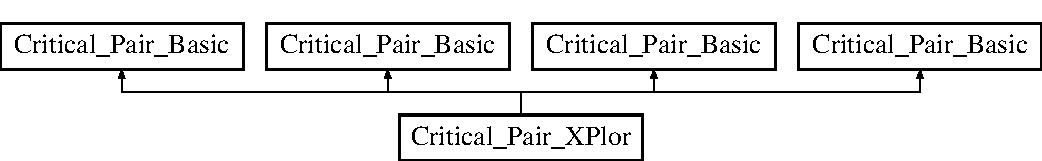
\includegraphics[height=1.917808cm]{group___g_b_computation}
\end{center}
\end{figure}
\subsubsection*{Public Member Functions}
\begin{Indent}\textbf{ Construction}\par
\begin{DoxyCompactItemize}
\item 
\mbox{\Hypertarget{group___g_b_computation_a54a4115589e1c46851167727b5d21578}\label{group___g_b_computation_a54a4115589e1c46851167727b5d21578}} 
\hyperlink{group___g_b_computation_a54a4115589e1c46851167727b5d21578}{Critical\+\_\+\+Pair\+\_\+\+Basic} (\hyperlink{group__polygroup_class_abstract___polynomial}{Abstract\+\_\+\+Polynomial} $\ast$f, \hyperlink{group__strategygroup_ga0ee6c8e033547330e6b89929730007f4}{Strategy\+Flags} strategy)
\begin{DoxyCompactList}\small\item\em create critical pair (f,0) for initial polynomial \end{DoxyCompactList}\item 
\mbox{\Hypertarget{group___g_b_computation_a393b8f7069c8e641a982ba4d704d349c}\label{group___g_b_computation_a393b8f7069c8e641a982ba4d704d349c}} 
\hyperlink{group___g_b_computation_a393b8f7069c8e641a982ba4d704d349c}{Critical\+\_\+\+Pair\+\_\+\+Basic} (\hyperlink{group__polygroup_class_abstract___polynomial}{Abstract\+\_\+\+Polynomial} $\ast$f, \hyperlink{group__polygroup_class_abstract___polynomial}{Abstract\+\_\+\+Polynomial} $\ast$g, \hyperlink{group__strategygroup_ga0ee6c8e033547330e6b89929730007f4}{Strategy\+Flags} strategy)
\begin{DoxyCompactList}\small\item\em create critical pair (f,g) for two polynomials \end{DoxyCompactList}\end{DoxyCompactItemize}
\end{Indent}
\begin{Indent}\textbf{ Destruction}\par
\begin{DoxyCompactItemize}
\item 
\mbox{\Hypertarget{group___g_b_computation_a5a3c9fa67ec45e8f9891d667c1ff43ec}\label{group___g_b_computation_a5a3c9fa67ec45e8f9891d667c1ff43ec}} 
virtual {\bfseries $\sim$\+Critical\+\_\+\+Pair\+\_\+\+Basic} ()
\end{DoxyCompactItemize}
\end{Indent}
\begin{Indent}\textbf{ Basic properties}\par
\begin{DoxyCompactItemize}
\item 
\mbox{\Hypertarget{group___g_b_computation_a621825e77a7f79234307be09d2fcf036}\label{group___g_b_computation_a621825e77a7f79234307be09d2fcf036}} 
bool \hyperlink{group___g_b_computation_a621825e77a7f79234307be09d2fcf036}{is\+\_\+generator} () const
\begin{DoxyCompactList}\small\item\em whether this pair is from a generator \end{DoxyCompactList}\item 
\mbox{\Hypertarget{group___g_b_computation_a6e251e3724fde2c610d921f93889eb67}\label{group___g_b_computation_a6e251e3724fde2c610d921f93889eb67}} 
const \hyperlink{group__polygroup_class_abstract___polynomial}{Abstract\+\_\+\+Polynomial} $\ast$ \hyperlink{group___g_b_computation_a6e251e3724fde2c610d921f93889eb67}{first} () const
\begin{DoxyCompactList}\small\item\em first polynomial in pair \end{DoxyCompactList}\item 
\mbox{\Hypertarget{group___g_b_computation_a06da1cbbe1451962b68f2bbf90855fae}\label{group___g_b_computation_a06da1cbbe1451962b68f2bbf90855fae}} 
const \hyperlink{group__polygroup_class_abstract___polynomial}{Abstract\+\_\+\+Polynomial} $\ast$ \hyperlink{group___g_b_computation_a06da1cbbe1451962b68f2bbf90855fae}{second} () const
\begin{DoxyCompactList}\small\item\em second polynomial in pair \end{DoxyCompactList}\item 
\mbox{\Hypertarget{group___g_b_computation_a336387d4ddd4f184399212599dbcb130}\label{group___g_b_computation_a336387d4ddd4f184399212599dbcb130}} 
const \hyperlink{group__polygroup_class_monomial}{Monomial} \& \hyperlink{group___g_b_computation_a336387d4ddd4f184399212599dbcb130}{lcm} () const
\begin{DoxyCompactList}\small\item\em lcm of leading monomials of polynomials \end{DoxyCompactList}\item 
\mbox{\Hypertarget{group___g_b_computation_a4b9daf511d0ae94c24a5a0b8aa07588b}\label{group___g_b_computation_a4b9daf511d0ae94c24a5a0b8aa07588b}} 
unsigned \hyperlink{group___g_b_computation_a4b9daf511d0ae94c24a5a0b8aa07588b}{lcm\+\_\+degree} (unsigned i) const
\begin{DoxyCompactList}\small\item\em degree of ith variable in lcm \end{DoxyCompactList}\item 
\mbox{\Hypertarget{group___g_b_computation_a714e1ea76b993148dd55b05979b4b874}\label{group___g_b_computation_a714e1ea76b993148dd55b05979b4b874}} 
const \hyperlink{group__polygroup_class_monomial}{Monomial} \& \hyperlink{group___g_b_computation_a714e1ea76b993148dd55b05979b4b874}{first\+\_\+multiplier} () const
\begin{DoxyCompactList}\small\item\em monomial needed to multiply first polynomial to \hyperlink{group___g_b_computation_a336387d4ddd4f184399212599dbcb130}{lcm()} \end{DoxyCompactList}\item 
\mbox{\Hypertarget{group___g_b_computation_abb08fb4bfc80732a92438cc6856503a1}\label{group___g_b_computation_abb08fb4bfc80732a92438cc6856503a1}} 
const \hyperlink{group__polygroup_class_monomial}{Monomial} \& \hyperlink{group___g_b_computation_abb08fb4bfc80732a92438cc6856503a1}{second\+\_\+multiplier} () const
\begin{DoxyCompactList}\small\item\em monomial needed to multiply second polynomial to \hyperlink{group___g_b_computation_a336387d4ddd4f184399212599dbcb130}{lcm()} \end{DoxyCompactList}\item 
\mbox{\Hypertarget{group___g_b_computation_a8fa18f909cc3b88af41a5796bd6c2424}\label{group___g_b_computation_a8fa18f909cc3b88af41a5796bd6c2424}} 
const \hyperlink{group__strategygroup_class_pair___strategy___data}{Pair\+\_\+\+Strategy\+\_\+\+Data} $\ast$ \hyperlink{group___g_b_computation_a8fa18f909cc3b88af41a5796bd6c2424}{pair\+\_\+key} () const
\begin{DoxyCompactList}\small\item\em strategy used for comparison of pairs \end{DoxyCompactList}\item 
virtual \hyperlink{group__polygroup_class_mutable___polynomial}{Mutable\+\_\+\+Polynomial} $\ast$ \hyperlink{group___g_b_computation_ab2dbac89b07b2acfad633a9de8f56fab}{s\+\_\+polynomial} ()
\begin{DoxyCompactList}\small\item\em to use only if s-\/polynomial is already computed by another method \end{DoxyCompactList}\end{DoxyCompactItemize}
\end{Indent}
\begin{Indent}\textbf{ Computation}\par
\begin{DoxyCompactItemize}
\item 
\mbox{\Hypertarget{group___g_b_computation_aedcb486aa7298a6ed5a1980890df0780}\label{group___g_b_computation_aedcb486aa7298a6ed5a1980890df0780}} 
virtual \hyperlink{group__polygroup_class_mutable___polynomial}{Mutable\+\_\+\+Polynomial} $\ast$ \hyperlink{group___g_b_computation_aedcb486aa7298a6ed5a1980890df0780}{s\+\_\+polynomial} (\hyperlink{group___g_b_computation_ga73257b8a2d5cc826853a71b77d0cebf2}{S\+Poly\+Creation\+Flags} method, \hyperlink{group__strategygroup_ga0ee6c8e033547330e6b89929730007f4}{Strategy\+Flags} strategy)
\begin{DoxyCompactList}\small\item\em creates the s-\/polynomial for \hyperlink{group___g_b_computation_a6e251e3724fde2c610d921f93889eb67}{first()} and \hyperlink{group___g_b_computation_a06da1cbbe1451962b68f2bbf90855fae}{second()} \end{DoxyCompactList}\end{DoxyCompactItemize}
\end{Indent}
\begin{Indent}\textbf{ Modification}\par
\begin{DoxyCompactItemize}
\item 
\mbox{\Hypertarget{group___g_b_computation_ad3ba8ead12784e3133eedf75e7601326}\label{group___g_b_computation_ad3ba8ead12784e3133eedf75e7601326}} 
virtual void \hyperlink{group___g_b_computation_ad3ba8ead12784e3133eedf75e7601326}{set\+\_\+spoly} (\hyperlink{group__polygroup_class_mutable___polynomial}{Mutable\+\_\+\+Polynomial} $\ast$\hyperlink{group___g_b_computation_ac80ca2c599a7c234e01e5377292d9a5a}{p})
\begin{DoxyCompactList}\small\item\em sets the s-\/polynomial to {\ttfamily p}, for explorer methods \end{DoxyCompactList}\end{DoxyCompactItemize}
\end{Indent}
\subsubsection*{Protected Attributes}
\begin{DoxyCompactItemize}
\item 
\mbox{\Hypertarget{group___g_b_computation_a638c1db1878db2e677986637f0b73d54}\label{group___g_b_computation_a638c1db1878db2e677986637f0b73d54}} 
\hyperlink{group__strategygroup_class_pair___strategy___data}{Pair\+\_\+\+Strategy\+\_\+\+Data} $\ast$ \hyperlink{group___g_b_computation_a638c1db1878db2e677986637f0b73d54}{key} = nullptr
\begin{DoxyCompactList}\small\item\em strategy used to sort critical pairs \end{DoxyCompactList}\item 
\mbox{\Hypertarget{group___g_b_computation_ac80ca2c599a7c234e01e5377292d9a5a}\label{group___g_b_computation_ac80ca2c599a7c234e01e5377292d9a5a}} 
\hyperlink{group__polygroup_class_abstract___polynomial}{Abstract\+\_\+\+Polynomial} $\ast$ \hyperlink{group___g_b_computation_ac80ca2c599a7c234e01e5377292d9a5a}{p}
\begin{DoxyCompactList}\small\item\em first polynomial in the critical pair \end{DoxyCompactList}\item 
\mbox{\Hypertarget{group___g_b_computation_a038d8389aa28cdbc63a3e132bd226cfc}\label{group___g_b_computation_a038d8389aa28cdbc63a3e132bd226cfc}} 
\hyperlink{group__polygroup_class_abstract___polynomial}{Abstract\+\_\+\+Polynomial} $\ast$ \hyperlink{group___g_b_computation_a038d8389aa28cdbc63a3e132bd226cfc}{q}
\begin{DoxyCompactList}\small\item\em second polynomial in the critical pair \end{DoxyCompactList}\item 
\mbox{\Hypertarget{group___g_b_computation_aa7ac66f9f3cceafd55a1fd0061335afc}\label{group___g_b_computation_aa7ac66f9f3cceafd55a1fd0061335afc}} 
\hyperlink{group__polygroup_class_mutable___polynomial}{Mutable\+\_\+\+Polynomial} $\ast$ \hyperlink{group___g_b_computation_aa7ac66f9f3cceafd55a1fd0061335afc}{s}
\begin{DoxyCompactList}\small\item\em S-\/polynomial. \end{DoxyCompactList}\item 
\mbox{\Hypertarget{group___g_b_computation_a9b232e6359525154a6d7865e607964bb}\label{group___g_b_computation_a9b232e6359525154a6d7865e607964bb}} 
\hyperlink{group__polygroup_class_monomial}{Monomial} \hyperlink{group___g_b_computation_a9b232e6359525154a6d7865e607964bb}{tp}
\begin{DoxyCompactList}\small\item\em monomial multiple of $p$ that produces $S$-\/polynomial \end{DoxyCompactList}\item 
\mbox{\Hypertarget{group___g_b_computation_a91d6dc4856d8fb137faf8ffe2b823ae8}\label{group___g_b_computation_a91d6dc4856d8fb137faf8ffe2b823ae8}} 
\hyperlink{group__polygroup_class_monomial}{Monomial} \hyperlink{group___g_b_computation_a91d6dc4856d8fb137faf8ffe2b823ae8}{tpq}
\begin{DoxyCompactList}\small\item\em lcm of leading monomials of $p$ and $q$ \end{DoxyCompactList}\item 
\mbox{\Hypertarget{group___g_b_computation_a7e67ffb4af6c13830c95253e464bc3a3}\label{group___g_b_computation_a7e67ffb4af6c13830c95253e464bc3a3}} 
\hyperlink{group__polygroup_class_monomial}{Monomial} \hyperlink{group___g_b_computation_a7e67ffb4af6c13830c95253e464bc3a3}{tq}
\begin{DoxyCompactList}\small\item\em monomial multiple of $q$ that produces $S$-\/polynomial \end{DoxyCompactList}\end{DoxyCompactItemize}
\subsubsection*{Friends}
\begin{Indent}\textbf{ I/O}\par
\begin{DoxyCompactItemize}
\item 
\mbox{\Hypertarget{group___g_b_computation_a142698d76b6358faf451f21bf929c993}\label{group___g_b_computation_a142698d76b6358faf451f21bf929c993}} 
ostream \& {\bfseries operator$<$$<$} (ostream \&, const \hyperlink{group___g_b_computation_class_critical___pair___basic}{Critical\+\_\+\+Pair\+\_\+\+Basic} \&)
\end{DoxyCompactItemize}
\end{Indent}


\paragraph{Member Function Documentation}
\mbox{\Hypertarget{group___g_b_computation_ab2dbac89b07b2acfad633a9de8f56fab}\label{group___g_b_computation_ab2dbac89b07b2acfad633a9de8f56fab}} 
\index{Critical\+\_\+\+Pair\+\_\+\+Basic@{Critical\+\_\+\+Pair\+\_\+\+Basic}!s\+\_\+polynomial@{s\+\_\+polynomial}}
\index{s\+\_\+polynomial@{s\+\_\+polynomial}!Critical\+\_\+\+Pair\+\_\+\+Basic@{Critical\+\_\+\+Pair\+\_\+\+Basic}}
\subparagraph{\texorpdfstring{s\+\_\+polynomial()}{s\_polynomial()}}
{\footnotesize\ttfamily virtual \hyperlink{group__polygroup_class_mutable___polynomial}{Mutable\+\_\+\+Polynomial}$\ast$ Critical\+\_\+\+Pair\+\_\+\+Basic\+::s\+\_\+polynomial (\begin{DoxyParamCaption}{ }\end{DoxyParamCaption})\hspace{0.3cm}{\ttfamily [inline]}, {\ttfamily [virtual]}}



to use only if s-\/polynomial is already computed by another method 

\begin{DoxyWarning}{Warning}
If you have not already created an s-\/polynomial using one of S\+Poly\+Creation\+Flags, then this returns {\ttfamily nullptr} and is useless. 
\end{DoxyWarning}
\begin{DoxyReturn}{Returns}
the s-\/polynomial of this pair 
\end{DoxyReturn}


Definition at line 113 of file critical\+\_\+pair.\+hpp.

\index{Critical\+\_\+\+Pair\+\_\+\+Dynamic@{Critical\+\_\+\+Pair\+\_\+\+Dynamic}}\label{class_critical___pair___dynamic}
\Hypertarget{group___g_b_computation_class_critical___pair___dynamic}
\subsubsection{class Critical\+\_\+\+Pair\+\_\+\+Dynamic}
Controls the creation of s-\/polynomials, specialized for the dynamic algorithm. 

\begin{DoxyAuthor}{Author}
John Perry 
\end{DoxyAuthor}
\begin{DoxyDate}{Date}
2016
\end{DoxyDate}
This class encapsulates the information necessary to create an $S$-\/polynomial, including the actual generation of an $S$-\/polynomial, though it does not retain that information. The main difference with {\ttfamily \hyperlink{group___g_b_computation_class_critical___pair___basic}{Critical\+\_\+\+Pair\+\_\+\+Basic}} is the enabling of late re-\/sorting. 

Definition at line 162 of file critical\+\_\+pair.\+hpp.

Inheritance diagram for Critical\+\_\+\+Pair\+\_\+\+Dynamic\+:\begin{figure}[H]
\begin{center}
\leavevmode
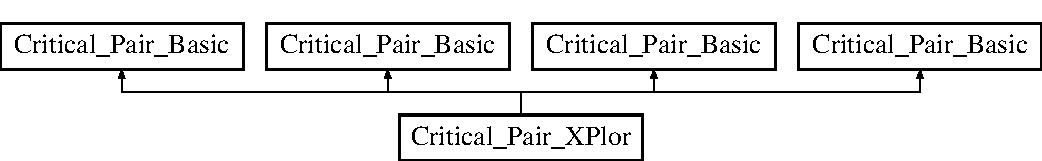
\includegraphics[height=2.000000cm]{group___g_b_computation}
\end{center}
\end{figure}
\subsubsection*{Public Member Functions}
\begin{Indent}\textbf{ Construction}\par
\begin{DoxyCompactItemize}
\item 
\mbox{\Hypertarget{group___g_b_computation_a121415e702ea63da6444839d9f59669a}\label{group___g_b_computation_a121415e702ea63da6444839d9f59669a}} 
\hyperlink{group___g_b_computation_a121415e702ea63da6444839d9f59669a}{Critical\+\_\+\+Pair\+\_\+\+Dynamic} (\hyperlink{group__polygroup_class_abstract___polynomial}{Abstract\+\_\+\+Polynomial} $\ast$f, \hyperlink{group__strategygroup_ga0ee6c8e033547330e6b89929730007f4}{Strategy\+Flags} strategy, \hyperlink{group__orderinggroup_class_weighted___ordering}{Weighted\+\_\+\+Ordering} $\ast$how\+\_\+to\+\_\+order)
\begin{DoxyCompactList}\small\item\em create critical pair (f,0) for initial polynomial, with given ordering \end{DoxyCompactList}\item 
\mbox{\Hypertarget{group___g_b_computation_afe29c049d24e98470ba7099d25a01b15}\label{group___g_b_computation_afe29c049d24e98470ba7099d25a01b15}} 
\hyperlink{group___g_b_computation_afe29c049d24e98470ba7099d25a01b15}{Critical\+\_\+\+Pair\+\_\+\+Dynamic} (\hyperlink{group__polygroup_class_abstract___polynomial}{Abstract\+\_\+\+Polynomial} $\ast$f, \hyperlink{group__polygroup_class_abstract___polynomial}{Abstract\+\_\+\+Polynomial} $\ast$g, \hyperlink{group__strategygroup_ga0ee6c8e033547330e6b89929730007f4}{Strategy\+Flags} strategy, \hyperlink{group__orderinggroup_class_weighted___ordering}{Weighted\+\_\+\+Ordering} $\ast$how\+\_\+to\+\_\+order)
\begin{DoxyCompactList}\small\item\em create critical pair (f,g) for two polynomials, with given ordering \end{DoxyCompactList}\end{DoxyCompactItemize}
\end{Indent}
\begin{Indent}\textbf{ Computation}\par
\begin{DoxyCompactItemize}
\item 
virtual \hyperlink{group__polygroup_class_mutable___polynomial}{Mutable\+\_\+\+Polynomial} $\ast$ \hyperlink{group___g_b_computation_a3146fa294ea814d5388e09b1c76c966b}{s\+\_\+polynomial} (\hyperlink{group___g_b_computation_ga73257b8a2d5cc826853a71b77d0cebf2}{S\+Poly\+Creation\+Flags} method, \hyperlink{group__strategygroup_ga0ee6c8e033547330e6b89929730007f4}{Strategy\+Flags} strategy)
\begin{DoxyCompactList}\small\item\em creates the s-\/polynomial for \hyperlink{group___g_b_computation_a6e251e3724fde2c610d921f93889eb67}{first()} and \hyperlink{group___g_b_computation_a06da1cbbe1451962b68f2bbf90855fae}{second()} \end{DoxyCompactList}\end{DoxyCompactItemize}
\end{Indent}
\begin{Indent}\textbf{ Basic properties}\par
\begin{DoxyCompactItemize}
\item 
\mbox{\Hypertarget{group___g_b_computation_afbdf7f7bc0d9332c3df08858b0803aed}\label{group___g_b_computation_afbdf7f7bc0d9332c3df08858b0803aed}} 
\hyperlink{group__orderinggroup_class_weighted___ordering}{Weighted\+\_\+\+Ordering} $\ast$ \hyperlink{group___g_b_computation_afbdf7f7bc0d9332c3df08858b0803aed}{how\+\_\+ordered} () const
\begin{DoxyCompactList}\small\item\em the ordering associated with this pair \end{DoxyCompactList}\end{DoxyCompactItemize}
\end{Indent}
\begin{Indent}\textbf{ Modification}\par
\begin{DoxyCompactItemize}
\item 
void \hyperlink{group___g_b_computation_aa9001ca49b2c2fd7d39384e4e70c5a6b}{change\+\_\+ordering} (\hyperlink{group__orderinggroup_class_weighted___ordering}{Weighted\+\_\+\+Ordering} $\ast$new\+\_\+order)
\begin{DoxyCompactList}\small\item\em change the ordering associated with this pair \end{DoxyCompactList}\end{DoxyCompactItemize}
\end{Indent}
\subsubsection*{Protected Attributes}
\begin{DoxyCompactItemize}
\item 
\mbox{\Hypertarget{group___g_b_computation_a29d3c615e66d3840c3aeb8ad9bc51647}\label{group___g_b_computation_a29d3c615e66d3840c3aeb8ad9bc51647}} 
\hyperlink{group__orderinggroup_class_weighted___ordering}{Weighted\+\_\+\+Ordering} $\ast$ \hyperlink{group___g_b_computation_a29d3c615e66d3840c3aeb8ad9bc51647}{ordering}
\begin{DoxyCompactList}\small\item\em the {\ttfamily \hyperlink{group__orderinggroup_class_monomial___ordering}{Monomial\+\_\+\+Ordering}} assigned to this pair --- might disagree with that of polynomials; they must be updated immediately if this is a generator; otherwise, update can wait until the critical pair is computed. \end{DoxyCompactList}\end{DoxyCompactItemize}
\subsubsection*{Friends}
\begin{Indent}\textbf{ I/O}\par
\begin{DoxyCompactItemize}
\item 
\mbox{\Hypertarget{group___g_b_computation_a3c0c965ed52ffe0faf759023605adaf2}\label{group___g_b_computation_a3c0c965ed52ffe0faf759023605adaf2}} 
ostream \& \hyperlink{group___g_b_computation_a3c0c965ed52ffe0faf759023605adaf2}{operator$<$$<$} (ostream \&, const \hyperlink{group___g_b_computation_class_critical___pair___dynamic}{Critical\+\_\+\+Pair\+\_\+\+Dynamic} \&)
\begin{DoxyCompactList}\small\item\em outputs the pair, and the ordering \end{DoxyCompactList}\end{DoxyCompactItemize}
\end{Indent}


\paragraph{Member Function Documentation}
\mbox{\Hypertarget{group___g_b_computation_aa9001ca49b2c2fd7d39384e4e70c5a6b}\label{group___g_b_computation_aa9001ca49b2c2fd7d39384e4e70c5a6b}} 
\index{Critical\+\_\+\+Pair\+\_\+\+Dynamic@{Critical\+\_\+\+Pair\+\_\+\+Dynamic}!change\+\_\+ordering@{change\+\_\+ordering}}
\index{change\+\_\+ordering@{change\+\_\+ordering}!Critical\+\_\+\+Pair\+\_\+\+Dynamic@{Critical\+\_\+\+Pair\+\_\+\+Dynamic}}
\subparagraph{\texorpdfstring{change\+\_\+ordering()}{change\_ordering()}}
{\footnotesize\ttfamily void Critical\+\_\+\+Pair\+\_\+\+Dynamic\+::change\+\_\+ordering (\begin{DoxyParamCaption}\item[{\hyperlink{group__orderinggroup_class_weighted___ordering}{Weighted\+\_\+\+Ordering} $\ast$}]{new\+\_\+order }\end{DoxyParamCaption})\hspace{0.3cm}{\ttfamily [inline]}}



change the ordering associated with this pair 

This is necessary at least for critical pairs where one polynomial is a generator that we have not yet computed. We delay re-\/sorting the polynomial until the s-\/polynomial's computation. 
\begin{DoxyParams}{Parameters}
{\em new\+\_\+order} & the new ordering for this critical pair \\
\hline
\end{DoxyParams}


Definition at line 234 of file critical\+\_\+pair.\+hpp.

\mbox{\Hypertarget{group___g_b_computation_a3146fa294ea814d5388e09b1c76c966b}\label{group___g_b_computation_a3146fa294ea814d5388e09b1c76c966b}} 
\index{Critical\+\_\+\+Pair\+\_\+\+Dynamic@{Critical\+\_\+\+Pair\+\_\+\+Dynamic}!s\+\_\+polynomial@{s\+\_\+polynomial}}
\index{s\+\_\+polynomial@{s\+\_\+polynomial}!Critical\+\_\+\+Pair\+\_\+\+Dynamic@{Critical\+\_\+\+Pair\+\_\+\+Dynamic}}
\subparagraph{\texorpdfstring{s\+\_\+polynomial()}{s\_polynomial()}}
{\footnotesize\ttfamily \hyperlink{group__polygroup_class_mutable___polynomial}{Mutable\+\_\+\+Polynomial} $\ast$ Critical\+\_\+\+Pair\+\_\+\+Dynamic\+::s\+\_\+polynomial (\begin{DoxyParamCaption}\item[{\hyperlink{group___g_b_computation_ga73257b8a2d5cc826853a71b77d0cebf2}{S\+Poly\+Creation\+Flags}}]{method,  }\item[{\hyperlink{group__strategygroup_ga0ee6c8e033547330e6b89929730007f4}{Strategy\+Flags}}]{strategy }\end{DoxyParamCaption})\hspace{0.3cm}{\ttfamily [virtual]}}



creates the s-\/polynomial for \hyperlink{group___g_b_computation_a6e251e3724fde2c610d921f93889eb67}{first()} and \hyperlink{group___g_b_computation_a06da1cbbe1451962b68f2bbf90855fae}{second()} 

If either \hyperlink{group___g_b_computation_a6e251e3724fde2c610d921f93889eb67}{first()} or \hyperlink{group___g_b_computation_a06da1cbbe1451962b68f2bbf90855fae}{second()} was sorted using an ordering different from the one assigned the pair, it is sorted anew. 
\begin{DoxyParams}{Parameters}
{\em method} & a flag for what structure to use while reducing the s-\/polynomial; see S\+Poly\+Creation\+Flags \\
\hline
{\em strategy} & a flag for which strategy to use in reduction; see Strategy\+Flags \\
\hline
\end{DoxyParams}
\begin{DoxyReturn}{Returns}
the generated s-\/polynomial 
\end{DoxyReturn}


Reimplemented from \hyperlink{group___g_b_computation_aedcb486aa7298a6ed5a1980890df0780}{Critical\+\_\+\+Pair\+\_\+\+Basic}.



Definition at line 152 of file critical\+\_\+pair.\+cpp.

\index{Critical\+\_\+\+Pair\+\_\+\+X\+Plor@{Critical\+\_\+\+Pair\+\_\+\+X\+Plor}}\label{class_critical___pair___x_plor}
\Hypertarget{group___g_b_computation_class_critical___pair___x_plor}
\subsubsection{class Critical\+\_\+\+Pair\+\_\+\+X\+Plor}
contains information on critical pairs by their index in the basis, in addition to the usual information 

Definition at line 46 of file algorithm\+\_\+buchberger\+\_\+explorer.\+cpp.

Inheritance diagram for Critical\+\_\+\+Pair\+\_\+\+X\+Plor\+:\begin{figure}[H]
\begin{center}
\leavevmode
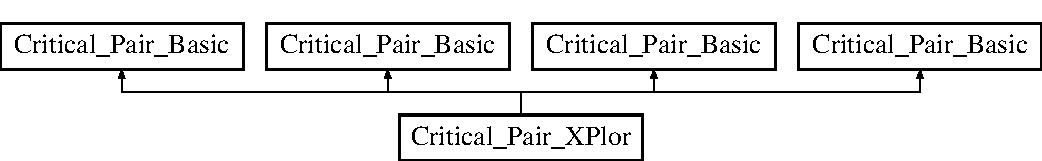
\includegraphics[height=2.000000cm]{group___g_b_computation}
\end{center}
\end{figure}
\subsubsection*{Public Member Functions}
\begin{Indent}\textbf{ Construction}\par
\begin{DoxyCompactItemize}
\item 
\mbox{\Hypertarget{group___g_b_computation_a056c7e030d1bcb86444bf52405482964}\label{group___g_b_computation_a056c7e030d1bcb86444bf52405482964}} 
\hyperlink{group___g_b_computation_a056c7e030d1bcb86444bf52405482964}{Critical\+\_\+\+Pair\+\_\+\+X\+Plor} (int i, \hyperlink{group__strategygroup_ga0ee6c8e033547330e6b89929730007f4}{Strategy\+Flags} strategy, \hyperlink{group__polygroup_class_abstract___polynomial}{Abstract\+\_\+\+Polynomial} $\ast$f)
\begin{DoxyCompactList}\small\item\em create critical pair (f,0) where f is at index {\ttfamily i} \end{DoxyCompactList}\item 
\mbox{\Hypertarget{group___g_b_computation_ab1d6ca591788b357af72ed85f94e4bd5}\label{group___g_b_computation_ab1d6ca591788b357af72ed85f94e4bd5}} 
\hyperlink{group___g_b_computation_ab1d6ca591788b357af72ed85f94e4bd5}{Critical\+\_\+\+Pair\+\_\+\+X\+Plor} (int i, int j, \hyperlink{group__strategygroup_ga0ee6c8e033547330e6b89929730007f4}{Strategy\+Flags} strategy, vector$<$ \hyperlink{group__polygroup_class_abstract___polynomial}{Abstract\+\_\+\+Polynomial} $\ast$$>$G)
\begin{DoxyCompactList}\small\item\em create critical pair (f,g) where f, g are at indices {\ttfamily i}, {\ttfamily j} \end{DoxyCompactList}\item 
\mbox{\Hypertarget{group___g_b_computation_a01353f6df8dacecfbee9a9cc546fb0cc}\label{group___g_b_computation_a01353f6df8dacecfbee9a9cc546fb0cc}} 
\hyperlink{group___g_b_computation_a01353f6df8dacecfbee9a9cc546fb0cc}{Critical\+\_\+\+Pair\+\_\+\+X\+Plor} (int i, \hyperlink{group__polygroup_class_abstract___polynomial}{Abstract\+\_\+\+Polynomial} $\ast$g, \hyperlink{group__strategygroup_ga0ee6c8e033547330e6b89929730007f4}{Strategy\+Flags} strategy, vector$<$ \hyperlink{group__polygroup_class_abstract___polynomial}{Abstract\+\_\+\+Polynomial} $\ast$$>$G)
\begin{DoxyCompactList}\small\item\em create critical pair (f,g) where f is at index {\ttfamily i} \end{DoxyCompactList}\item 
\mbox{\Hypertarget{group___g_b_computation_ac1564546db9b4736444a614970c1796d}\label{group___g_b_computation_ac1564546db9b4736444a614970c1796d}} 
\hyperlink{group___g_b_computation_ac1564546db9b4736444a614970c1796d}{Critical\+\_\+\+Pair\+\_\+\+X\+Plor} (int i, unsigned strategy, \hyperlink{group__polygroup_class_abstract___polynomial}{Abstract\+\_\+\+Polynomial} $\ast$f)
\begin{DoxyCompactList}\small\item\em create critical pair (f,0) where f is at index {\ttfamily i} \end{DoxyCompactList}\item 
\mbox{\Hypertarget{group___g_b_computation_af5d0947e70b4070f796f1b0d8ce75484}\label{group___g_b_computation_af5d0947e70b4070f796f1b0d8ce75484}} 
\hyperlink{group___g_b_computation_af5d0947e70b4070f796f1b0d8ce75484}{Critical\+\_\+\+Pair\+\_\+\+X\+Plor} (int i, int j, unsigned strategy, vector$<$ \hyperlink{group__polygroup_class_abstract___polynomial}{Abstract\+\_\+\+Polynomial} $\ast$$>$G)
\begin{DoxyCompactList}\small\item\em create critical pair (f,g) where f, g are at indices {\ttfamily i}, {\ttfamily j} \end{DoxyCompactList}\item 
\mbox{\Hypertarget{group___g_b_computation_a1cafe8e84ec3bee5e63370b7b815ba71}\label{group___g_b_computation_a1cafe8e84ec3bee5e63370b7b815ba71}} 
\hyperlink{group___g_b_computation_a1cafe8e84ec3bee5e63370b7b815ba71}{Critical\+\_\+\+Pair\+\_\+\+X\+Plor} (int i, \hyperlink{group__polygroup_class_abstract___polynomial}{Abstract\+\_\+\+Polynomial} $\ast$g, unsigned strategy, vector$<$ \hyperlink{group__polygroup_class_abstract___polynomial}{Abstract\+\_\+\+Polynomial} $\ast$$>$G)
\begin{DoxyCompactList}\small\item\em create critical pair (f,g) where f is at index {\ttfamily i} \end{DoxyCompactList}\item 
\mbox{\Hypertarget{group___g_b_computation_ac1564546db9b4736444a614970c1796d}\label{group___g_b_computation_ac1564546db9b4736444a614970c1796d}} 
\hyperlink{group___g_b_computation_ac1564546db9b4736444a614970c1796d}{Critical\+\_\+\+Pair\+\_\+\+X\+Plor} (int i, unsigned strategy, \hyperlink{group__polygroup_class_abstract___polynomial}{Abstract\+\_\+\+Polynomial} $\ast$f)
\begin{DoxyCompactList}\small\item\em create critical pair (f,0) where f is at index {\ttfamily i} \end{DoxyCompactList}\item 
\mbox{\Hypertarget{group___g_b_computation_af5d0947e70b4070f796f1b0d8ce75484}\label{group___g_b_computation_af5d0947e70b4070f796f1b0d8ce75484}} 
\hyperlink{group___g_b_computation_af5d0947e70b4070f796f1b0d8ce75484}{Critical\+\_\+\+Pair\+\_\+\+X\+Plor} (int i, int j, unsigned strategy, vector$<$ \hyperlink{group__polygroup_class_abstract___polynomial}{Abstract\+\_\+\+Polynomial} $\ast$$>$G)
\begin{DoxyCompactList}\small\item\em create critical pair (f,g) where f, g are at indices {\ttfamily i}, {\ttfamily j} \end{DoxyCompactList}\item 
\mbox{\Hypertarget{group___g_b_computation_a1cafe8e84ec3bee5e63370b7b815ba71}\label{group___g_b_computation_a1cafe8e84ec3bee5e63370b7b815ba71}} 
\hyperlink{group___g_b_computation_a1cafe8e84ec3bee5e63370b7b815ba71}{Critical\+\_\+\+Pair\+\_\+\+X\+Plor} (int i, \hyperlink{group__polygroup_class_abstract___polynomial}{Abstract\+\_\+\+Polynomial} $\ast$g, unsigned strategy, vector$<$ \hyperlink{group__polygroup_class_abstract___polynomial}{Abstract\+\_\+\+Polynomial} $\ast$$>$G)
\begin{DoxyCompactList}\small\item\em create critical pair (f,g) where f is at index {\ttfamily i} \end{DoxyCompactList}\end{DoxyCompactItemize}
\end{Indent}
\begin{Indent}\textbf{ Basic properties}\par
\begin{DoxyCompactItemize}
\item 
\mbox{\Hypertarget{group___g_b_computation_ac163e7707177e0c8566903ffdedea821}\label{group___g_b_computation_ac163e7707177e0c8566903ffdedea821}} 
int \hyperlink{group___g_b_computation_ac163e7707177e0c8566903ffdedea821}{first\+\_\+index} ()
\begin{DoxyCompactList}\small\item\em returns index of first polynomial in pair \end{DoxyCompactList}\item 
\mbox{\Hypertarget{group___g_b_computation_a201f10149987060902a3999e4db201b9}\label{group___g_b_computation_a201f10149987060902a3999e4db201b9}} 
int \hyperlink{group___g_b_computation_a201f10149987060902a3999e4db201b9}{second\+\_\+index} ()
\begin{DoxyCompactList}\small\item\em returns index of second polynomial in pair \end{DoxyCompactList}\item 
\mbox{\Hypertarget{group___g_b_computation_a85d34fcde810b942744433d1311ac331}\label{group___g_b_computation_a85d34fcde810b942744433d1311ac331}} 
D\+E\+G\+\_\+\+T\+Y\+PE \hyperlink{group___g_b_computation_a85d34fcde810b942744433d1311ac331}{sugar} ()
\begin{DoxyCompactList}\small\item\em returns sugar of this pair; use O\+N\+LY if with sugar strategy \end{DoxyCompactList}\item 
\mbox{\Hypertarget{group___g_b_computation_ac163e7707177e0c8566903ffdedea821}\label{group___g_b_computation_ac163e7707177e0c8566903ffdedea821}} 
int \hyperlink{group___g_b_computation_ac163e7707177e0c8566903ffdedea821}{first\+\_\+index} ()
\begin{DoxyCompactList}\small\item\em returns index of first polynomial in pair \end{DoxyCompactList}\item 
\mbox{\Hypertarget{group___g_b_computation_a201f10149987060902a3999e4db201b9}\label{group___g_b_computation_a201f10149987060902a3999e4db201b9}} 
int \hyperlink{group___g_b_computation_a201f10149987060902a3999e4db201b9}{second\+\_\+index} ()
\begin{DoxyCompactList}\small\item\em returns index of second polynomial in pair \end{DoxyCompactList}\item 
\mbox{\Hypertarget{group___g_b_computation_a85d34fcde810b942744433d1311ac331}\label{group___g_b_computation_a85d34fcde810b942744433d1311ac331}} 
D\+E\+G\+\_\+\+T\+Y\+PE \hyperlink{group___g_b_computation_a85d34fcde810b942744433d1311ac331}{sugar} ()
\begin{DoxyCompactList}\small\item\em returns sugar of this pair; use O\+N\+LY if with sugar strategy \end{DoxyCompactList}\item 
\mbox{\Hypertarget{group___g_b_computation_ac163e7707177e0c8566903ffdedea821}\label{group___g_b_computation_ac163e7707177e0c8566903ffdedea821}} 
int \hyperlink{group___g_b_computation_ac163e7707177e0c8566903ffdedea821}{first\+\_\+index} ()
\begin{DoxyCompactList}\small\item\em returns index of first polynomial in pair \end{DoxyCompactList}\item 
\mbox{\Hypertarget{group___g_b_computation_a201f10149987060902a3999e4db201b9}\label{group___g_b_computation_a201f10149987060902a3999e4db201b9}} 
int \hyperlink{group___g_b_computation_a201f10149987060902a3999e4db201b9}{second\+\_\+index} ()
\begin{DoxyCompactList}\small\item\em returns index of second polynomial in pair \end{DoxyCompactList}\item 
\mbox{\Hypertarget{group___g_b_computation_a85d34fcde810b942744433d1311ac331}\label{group___g_b_computation_a85d34fcde810b942744433d1311ac331}} 
D\+E\+G\+\_\+\+T\+Y\+PE \hyperlink{group___g_b_computation_a85d34fcde810b942744433d1311ac331}{sugar} ()
\begin{DoxyCompactList}\small\item\em returns sugar of this pair; use O\+N\+LY if with sugar strategy \end{DoxyCompactList}\end{DoxyCompactItemize}
\end{Indent}
\begin{Indent}\textbf{ Multiprocessing data}\par
\begin{DoxyCompactItemize}
\item 
\mbox{\Hypertarget{group___g_b_computation_a4c0085660583e247f354735ee900f2d3}\label{group___g_b_computation_a4c0085660583e247f354735ee900f2d3}} 
void \hyperlink{group___g_b_computation_a4c0085660583e247f354735ee900f2d3}{set\+\_\+processor} (int i)
\begin{DoxyCompactList}\small\item\em record that this pair is assigned to processor {\ttfamily i} \end{DoxyCompactList}\item 
\mbox{\Hypertarget{group___g_b_computation_a1f07b8a991c138ad6c8de5deeb64ece6}\label{group___g_b_computation_a1f07b8a991c138ad6c8de5deeb64ece6}} 
int \hyperlink{group___g_b_computation_a1f07b8a991c138ad6c8de5deeb64ece6}{get\+\_\+processor} ()
\begin{DoxyCompactList}\small\item\em query whether this pair is assigned to a processor, and which (nonnegative value indicates assignment, and to which) \end{DoxyCompactList}\item 
\mbox{\Hypertarget{group___g_b_computation_a4c0085660583e247f354735ee900f2d3}\label{group___g_b_computation_a4c0085660583e247f354735ee900f2d3}} 
void \hyperlink{group___g_b_computation_a4c0085660583e247f354735ee900f2d3}{set\+\_\+processor} (int i)
\begin{DoxyCompactList}\small\item\em record that this pair is assigned to processor {\ttfamily i} \end{DoxyCompactList}\item 
\mbox{\Hypertarget{group___g_b_computation_a1f07b8a991c138ad6c8de5deeb64ece6}\label{group___g_b_computation_a1f07b8a991c138ad6c8de5deeb64ece6}} 
int \hyperlink{group___g_b_computation_a1f07b8a991c138ad6c8de5deeb64ece6}{get\+\_\+processor} ()
\begin{DoxyCompactList}\small\item\em query whether this pair is assigned to a processor, and which (nonnegative value indicates assignment, and to which) \end{DoxyCompactList}\item 
\mbox{\Hypertarget{group___g_b_computation_a4c0085660583e247f354735ee900f2d3}\label{group___g_b_computation_a4c0085660583e247f354735ee900f2d3}} 
void \hyperlink{group___g_b_computation_a4c0085660583e247f354735ee900f2d3}{set\+\_\+processor} (int i)
\begin{DoxyCompactList}\small\item\em record that this pair is assigned to processor {\ttfamily i} \end{DoxyCompactList}\item 
\mbox{\Hypertarget{group___g_b_computation_a1f07b8a991c138ad6c8de5deeb64ece6}\label{group___g_b_computation_a1f07b8a991c138ad6c8de5deeb64ece6}} 
int \hyperlink{group___g_b_computation_a1f07b8a991c138ad6c8de5deeb64ece6}{get\+\_\+processor} ()
\begin{DoxyCompactList}\small\item\em query whether this pair is assigned to a processor, and which (nonnegative value indicates assignment, and to which) \end{DoxyCompactList}\end{DoxyCompactItemize}
\end{Indent}
\subsubsection*{Protected Attributes}
\begin{DoxyCompactItemize}
\item 
\mbox{\Hypertarget{group___g_b_computation_a815645cd7956540b6980868654e149a3}\label{group___g_b_computation_a815645cd7956540b6980868654e149a3}} 
int \hyperlink{group___g_b_computation_a815645cd7956540b6980868654e149a3}{pi}
\begin{DoxyCompactList}\small\item\em first polynomial in the critical pair \end{DoxyCompactList}\item 
\mbox{\Hypertarget{group___g_b_computation_a4e0a3c515ad3d9e29cec832d95ab2caa}\label{group___g_b_computation_a4e0a3c515ad3d9e29cec832d95ab2caa}} 
int \hyperlink{group___g_b_computation_a4e0a3c515ad3d9e29cec832d95ab2caa}{proc}
\begin{DoxyCompactList}\small\item\em processor to which this pair has been assigned \end{DoxyCompactList}\item 
\mbox{\Hypertarget{group___g_b_computation_a14a644d6decf4147a78dbaa85612130a}\label{group___g_b_computation_a14a644d6decf4147a78dbaa85612130a}} 
int \hyperlink{group___g_b_computation_a14a644d6decf4147a78dbaa85612130a}{qi}
\begin{DoxyCompactList}\small\item\em second polynomial in the critical pair \end{DoxyCompactList}\end{DoxyCompactItemize}
\index{Dynamic\+\_\+\+Engine\+::\+P\+P\+\_\+\+With\+\_\+\+Ideal@{Dynamic\+\_\+\+Engine\+::\+P\+P\+\_\+\+With\+\_\+\+Ideal}}\label{class_dynamic___engine_1_1_p_p___with___ideal}
\Hypertarget{group___g_b_computation_class_dynamic___engine_1_1_p_p___with___ideal}
\subsubsection{class Dynamic\+\_\+\+Engine\+:\+:P\+P\+\_\+\+With\+\_\+\+Ideal}
Used to associate a potential leading power product with the resulting monomial ideal if it were chosen as the actual leading power product. 

\begin{DoxyAuthor}{Author}
John Perry 
\end{DoxyAuthor}
\begin{DoxyDate}{Date}
2014 
\end{DoxyDate}


Definition at line 124 of file dynamic\+\_\+engine.\+hpp.

\subsubsection*{Public Member Functions}
\begin{Indent}\textbf{ Construction}\par
\begin{DoxyCompactItemize}
\item 
\hyperlink{group___g_b_computation_ab79e52cd576b29fc48e7d9ad49303ae7}{P\+P\+\_\+\+With\+\_\+\+Ideal} (\hyperlink{group__polygroup_class_monomial}{Monomial} u, const list$<$ \hyperlink{group__polygroup_class_monomial}{Monomial} $>$ \&F, \hyperlink{group___c_l_s_solvers_class_l_p___solvers_1_1_ray}{Ray} \&w, const list$<$ \hyperlink{group___g_b_computation_class_critical___pair___dynamic}{Critical\+\_\+\+Pair\+\_\+\+Dynamic} $\ast$$>$ \&P, const \hyperlink{group__polygroup_class_dense___univariate___integer___polynomial}{Dense\+\_\+\+Univariate\+\_\+\+Integer\+\_\+\+Polynomial} $\ast$h=nullptr)
\begin{DoxyCompactList}\small\item\em Construct a monomial/ideal pair. \end{DoxyCompactList}\item 
\mbox{\Hypertarget{group___g_b_computation_ac71ad235934d824958a14443be77789e}\label{group___g_b_computation_ac71ad235934d824958a14443be77789e}} 
\hyperlink{group___g_b_computation_ac71ad235934d824958a14443be77789e}{P\+P\+\_\+\+With\+\_\+\+Ideal} (const \hyperlink{group___g_b_computation_class_dynamic___engine_1_1_p_p___with___ideal}{P\+P\+\_\+\+With\+\_\+\+Ideal} \&PI)
\begin{DoxyCompactList}\small\item\em copy constructor \end{DoxyCompactList}\end{DoxyCompactItemize}
\end{Indent}
\begin{Indent}\textbf{ Destruction}\par
\begin{DoxyCompactItemize}
\item 
\mbox{\Hypertarget{group___g_b_computation_a1dd0ce9a355f10837a180b1599a2666f}\label{group___g_b_computation_a1dd0ce9a355f10837a180b1599a2666f}} 
\hyperlink{group___g_b_computation_a1dd0ce9a355f10837a180b1599a2666f}{$\sim$\+P\+P\+\_\+\+With\+\_\+\+Ideal} ()
\begin{DoxyCompactList}\small\item\em does nothing the default wouldn\textquotesingle{}t do \end{DoxyCompactList}\end{DoxyCompactItemize}
\end{Indent}
\begin{Indent}\textbf{ Basic properties}\par
\begin{DoxyCompactItemize}
\item 
\mbox{\Hypertarget{group___g_b_computation_a0b70c63442c37067103f9939b17ef4ec}\label{group___g_b_computation_a0b70c63442c37067103f9939b17ef4ec}} 
const \hyperlink{group__polygroup_class_monomial}{Monomial} \& \hyperlink{group___g_b_computation_a0b70c63442c37067103f9939b17ef4ec}{get\+\_\+pp} () const
\begin{DoxyCompactList}\small\item\em the leading monomial being added to the ideal \end{DoxyCompactList}\item 
\mbox{\Hypertarget{group___g_b_computation_acb57c1467a4d6e622143057fde1ba1b6}\label{group___g_b_computation_acb57c1467a4d6e622143057fde1ba1b6}} 
const \hyperlink{group__polygroup_class_monomial___ideal}{Monomial\+\_\+\+Ideal} \& \hyperlink{group___g_b_computation_acb57c1467a4d6e622143057fde1ba1b6}{get\+\_\+ideal} () const
\begin{DoxyCompactList}\small\item\em the old ideal of leading monomials \end{DoxyCompactList}\item 
\mbox{\Hypertarget{group___g_b_computation_a9d01761e8d285ddbaa35214d8214a74b}\label{group___g_b_computation_a9d01761e8d285ddbaa35214d8214a74b}} 
\hyperlink{group___c_l_s_solvers_class_l_p___solvers_1_1_ray}{Ray} \hyperlink{group___g_b_computation_a9d01761e8d285ddbaa35214d8214a74b}{get\+\_\+ordering} ()
\begin{DoxyCompactList}\small\item\em the current monomial ordering \end{DoxyCompactList}\item 
\mbox{\Hypertarget{group___g_b_computation_acc39727c4e1ef77c8fb74bca7955e9c4}\label{group___g_b_computation_acc39727c4e1ef77c8fb74bca7955e9c4}} 
const map$<$ D\+E\+G\+\_\+\+T\+Y\+PE, unsigned long $>$ \& \hyperlink{group___g_b_computation_acc39727c4e1ef77c8fb74bca7955e9c4}{get\+\_\+inc\+\_\+betti} (bool graded=false)
\begin{DoxyCompactList}\small\item\em the incremental Betti numbers obtained by adding the monomial to the ideal \end{DoxyCompactList}\item 
\mbox{\Hypertarget{group___g_b_computation_a1b8a9832df7be67f0e623870433577f8}\label{group___g_b_computation_a1b8a9832df7be67f0e623870433577f8}} 
\hyperlink{group__polygroup_class_dense___univariate___integer___polynomial}{Dense\+\_\+\+Univariate\+\_\+\+Integer\+\_\+\+Polynomial} $\ast$ \hyperlink{group___g_b_computation_a1b8a9832df7be67f0e623870433577f8}{get\+\_\+hilbert\+\_\+numerator} (bool graded=false)
\begin{DoxyCompactList}\small\item\em the Hilbert numerator obtained by adding the monomial to the ideal (numerator is {\itshape not} reduced) \end{DoxyCompactList}\item 
\mbox{\Hypertarget{group___g_b_computation_a1ad52b5a6782aa3e1434f7d4084c289f}\label{group___g_b_computation_a1ad52b5a6782aa3e1434f7d4084c289f}} 
\hyperlink{group__polygroup_class_dense___univariate___integer___polynomial}{Dense\+\_\+\+Univariate\+\_\+\+Integer\+\_\+\+Polynomial} $\ast$ \hyperlink{group___g_b_computation_a1ad52b5a6782aa3e1434f7d4084c289f}{get\+\_\+hilbert\+\_\+reduced\+\_\+numerator} (bool graded=false)
\begin{DoxyCompactList}\small\item\em the Hilbert numerator obtained by adding the monomial to the ideal (numerator {\itshape is} reduced) \end{DoxyCompactList}\item 
\mbox{\Hypertarget{group___g_b_computation_a63962938c3dfef78afe80e4e86eb9c78}\label{group___g_b_computation_a63962938c3dfef78afe80e4e86eb9c78}} 
\hyperlink{group__polygroup_class_dense___univariate___rational___polynomial}{Dense\+\_\+\+Univariate\+\_\+\+Rational\+\_\+\+Polynomial} $\ast$ \hyperlink{group___g_b_computation_a63962938c3dfef78afe80e4e86eb9c78}{get\+\_\+hilbert\+\_\+polynomial} ()
\begin{DoxyCompactList}\small\item\em the Hilbert polynomial obtained by adding the monomial to the ideal \end{DoxyCompactList}\item 
\mbox{\Hypertarget{group___g_b_computation_afb9a43c24f2d0405d1c60e12983c8003}\label{group___g_b_computation_afb9a43c24f2d0405d1c60e12983c8003}} 
int \hyperlink{group___g_b_computation_afb9a43c24f2d0405d1c60e12983c8003}{how\+\_\+many\+\_\+new\+\_\+pairs} () const
\begin{DoxyCompactList}\small\item\em estimate of the number of new critical pairs generated by adding the monomial to the ideal \end{DoxyCompactList}\item 
\mbox{\Hypertarget{group___g_b_computation_a68c0ece8174abdb6d2955d63f04cd437}\label{group___g_b_computation_a68c0ece8174abdb6d2955d63f04cd437}} 
int \hyperlink{group___g_b_computation_a68c0ece8174abdb6d2955d63f04cd437}{deg\+\_\+of\+\_\+new\+\_\+pairs} () const
\begin{DoxyCompactList}\small\item\em the degree of the new critical pairs generated by adding the monomial to the ideal \end{DoxyCompactList}\item 
\mbox{\Hypertarget{group___g_b_computation_addbeaeb67edfe33d4b4d71d7a4aa1aac}\label{group___g_b_computation_addbeaeb67edfe33d4b4d71d7a4aa1aac}} 
int \hyperlink{group___g_b_computation_addbeaeb67edfe33d4b4d71d7a4aa1aac}{get\+\_\+difference\+\_\+in\+\_\+degree} ()
\begin{DoxyCompactList}\small\item\em computes the difference in degree between the first and last monomials of the ideal \end{DoxyCompactList}\end{DoxyCompactItemize}
\end{Indent}
\begin{Indent}\textbf{ Modification}\par
\begin{DoxyCompactItemize}
\item 
\mbox{\Hypertarget{group___g_b_computation_abedc9cad9413fc7727e1b93d6eea16af}\label{group___g_b_computation_abedc9cad9413fc7727e1b93d6eea16af}} 
void \hyperlink{group___g_b_computation_abedc9cad9413fc7727e1b93d6eea16af}{compute\+\_\+number\+\_\+new\+\_\+pairs} ()
\begin{DoxyCompactList}\small\item\em Computes the number of critical pairs the monomial would add. \end{DoxyCompactList}\item 
\mbox{\Hypertarget{group___g_b_computation_a20bb441439236bcce2d9e87b8486553f}\label{group___g_b_computation_a20bb441439236bcce2d9e87b8486553f}} 
void \hyperlink{group___g_b_computation_a20bb441439236bcce2d9e87b8486553f}{set\+\_\+hilbert\+\_\+numerator} (\hyperlink{group__polygroup_class_dense___univariate___integer___polynomial}{Dense\+\_\+\+Univariate\+\_\+\+Integer\+\_\+\+Polynomial} $\ast$h)
\begin{DoxyCompactList}\small\item\em assigns a value to the hilbert numerator when it's already known \end{DoxyCompactList}\end{DoxyCompactItemize}
\end{Indent}
\subsubsection*{Protected Attributes}
\begin{DoxyCompactItemize}
\item 
\mbox{\Hypertarget{group___g_b_computation_a812c0be78a80ef2ecdd76e944a310363}\label{group___g_b_computation_a812c0be78a80ef2ecdd76e944a310363}} 
\hyperlink{group__polygroup_class_monomial___ideal}{Monomial\+\_\+\+Ideal} \hyperlink{group___g_b_computation_a812c0be78a80ef2ecdd76e944a310363}{I}
\begin{DoxyCompactList}\small\item\em the ideal of leading terms \end{DoxyCompactList}\item 
\mbox{\Hypertarget{group___g_b_computation_a4fa101d6caf52005d20e4398c5ff5607}\label{group___g_b_computation_a4fa101d6caf52005d20e4398c5ff5607}} 
int \hyperlink{group___g_b_computation_a4fa101d6caf52005d20e4398c5ff5607}{max\+\_\+deg}
\begin{DoxyCompactList}\small\item\em minimum weighted degree of monomials in ideal \end{DoxyCompactList}\item 
\mbox{\Hypertarget{group___g_b_computation_ae0ede63491bf929c811c31d8ecf1051e}\label{group___g_b_computation_ae0ede63491bf929c811c31d8ecf1051e}} 
int \hyperlink{group___g_b_computation_ae0ede63491bf929c811c31d8ecf1051e}{min\+\_\+deg}
\begin{DoxyCompactList}\small\item\em minimum weighted degree of monomials in ideal \end{DoxyCompactList}\item 
\mbox{\Hypertarget{group___g_b_computation_a79e7e4059e2ea811bc14a4c02de96c52}\label{group___g_b_computation_a79e7e4059e2ea811bc14a4c02de96c52}} 
int \hyperlink{group___g_b_computation_a79e7e4059e2ea811bc14a4c02de96c52}{num\+\_\+new\+\_\+pairs}
\begin{DoxyCompactList}\small\item\em estimate of number of new pairs \end{DoxyCompactList}\item 
\mbox{\Hypertarget{group___g_b_computation_ad4bc39f15f722a821f59db51b48a5d0f}\label{group___g_b_computation_ad4bc39f15f722a821f59db51b48a5d0f}} 
\hyperlink{group___c_l_s_solvers_class_l_p___solvers_1_1_ray}{Ray} \hyperlink{group___g_b_computation_ad4bc39f15f722a821f59db51b48a5d0f}{ordering}
\begin{DoxyCompactList}\small\item\em the current ordering of the Gr\"{o}bner basis computation \end{DoxyCompactList}\item 
\mbox{\Hypertarget{group___g_b_computation_a9254ab1c3c33afeb73786f3a10719e3f}\label{group___g_b_computation_a9254ab1c3c33afeb73786f3a10719e3f}} 
const list$<$ \hyperlink{group___g_b_computation_class_critical___pair___dynamic}{Critical\+\_\+\+Pair\+\_\+\+Dynamic} $\ast$ $>$ \& \hyperlink{group___g_b_computation_a9254ab1c3c33afeb73786f3a10719e3f}{pairs}
\begin{DoxyCompactList}\small\item\em the list of critical pairs of $I$ at this point in the algorithm \end{DoxyCompactList}\item 
\mbox{\Hypertarget{group___g_b_computation_abbb33a00772961f2fa9d851dae8a2e07}\label{group___g_b_computation_abbb33a00772961f2fa9d851dae8a2e07}} 
\hyperlink{group__polygroup_class_monomial}{Monomial} \hyperlink{group___g_b_computation_abbb33a00772961f2fa9d851dae8a2e07}{t}
\begin{DoxyCompactList}\small\item\em the last monomial added to $I$ \end{DoxyCompactList}\end{DoxyCompactItemize}


\paragraph{Constructor \& Destructor Documentation}
\mbox{\Hypertarget{group___g_b_computation_ab79e52cd576b29fc48e7d9ad49303ae7}\label{group___g_b_computation_ab79e52cd576b29fc48e7d9ad49303ae7}} 
\index{Dynamic\+\_\+\+Engine\+::\+P\+P\+\_\+\+With\+\_\+\+Ideal@{Dynamic\+\_\+\+Engine\+::\+P\+P\+\_\+\+With\+\_\+\+Ideal}!P\+P\+\_\+\+With\+\_\+\+Ideal@{P\+P\+\_\+\+With\+\_\+\+Ideal}}
\index{P\+P\+\_\+\+With\+\_\+\+Ideal@{P\+P\+\_\+\+With\+\_\+\+Ideal}!Dynamic\+\_\+\+Engine\+::\+P\+P\+\_\+\+With\+\_\+\+Ideal@{Dynamic\+\_\+\+Engine\+::\+P\+P\+\_\+\+With\+\_\+\+Ideal}}
\subparagraph{\texorpdfstring{P\+P\+\_\+\+With\+\_\+\+Ideal()}{PP\_With\_Ideal()}}
{\footnotesize\ttfamily Dynamic\+\_\+\+Engine\+::\+P\+P\+\_\+\+With\+\_\+\+Ideal\+::\+P\+P\+\_\+\+With\+\_\+\+Ideal (\begin{DoxyParamCaption}\item[{\hyperlink{group__polygroup_class_monomial}{Monomial}}]{u,  }\item[{const list$<$ \hyperlink{group__polygroup_class_monomial}{Monomial} $>$ \&}]{F,  }\item[{\hyperlink{group___c_l_s_solvers_class_l_p___solvers_1_1_ray}{Ray} \&}]{w,  }\item[{const list$<$ \hyperlink{group___g_b_computation_class_critical___pair___dynamic}{Critical\+\_\+\+Pair\+\_\+\+Dynamic} $\ast$$>$ \&}]{P,  }\item[{const \hyperlink{group__polygroup_class_dense___univariate___integer___polynomial}{Dense\+\_\+\+Univariate\+\_\+\+Integer\+\_\+\+Polynomial} $\ast$}]{h = {\ttfamily nullptr} }\end{DoxyParamCaption})\hspace{0.3cm}{\ttfamily [inline]}}



Construct a monomial/ideal pair. 


\begin{DoxyParams}{Parameters}
{\em u} & proposed new \hyperlink{group__polygroup_class_monomial}{Monomial} for ideal \\
\hline
{\em F} & current ideal \\
\hline
{\em w} & current monomial ordering \\
\hline
{\em P} & current list of critical pairs \\
\hline
{\em h} & unreduced Hilbert numerator of {\ttfamily F} (does not verify correctness) \\
\hline
\end{DoxyParams}


Definition at line 136 of file dynamic\+\_\+engine.\+hpp.

\index{F4\+\_\+\+Reduction\+\_\+\+Data@{F4\+\_\+\+Reduction\+\_\+\+Data}}\label{class_f4___reduction___data}
\Hypertarget{group___g_b_computation_class_f4___reduction___data}
\subsubsection{class F4\+\_\+\+Reduction\+\_\+\+Data}
Implementation of Faug\`{e}re's F4 algorithm. 

Currently computes a Gr\"{o}bner basis by selecting several s-\/polynomials of lowest lcm degree. Data is stored in a semi-\/sparse matrix format, with each row a contiguous array of entries ({\ttfamily A}). Each row of {\ttfamily A} begins at the position indicated by the corresponding {\ttfamily offset}, and its first non-\/zero entry appears at the position indicated by the corresponding {\ttfamily head}. So the leading coefficient of the polynomial in row {\ttfamily k} appears in {\ttfamily A\mbox{[}head\mbox{[}k\mbox{]}\mbox{]}} and the leading monomial appears in {\ttfamily M\mbox{[}offset\mbox{[}k\mbox{]}+head\mbox{[}k\mbox{]}\mbox{]}}. Starting from {\ttfamily head\mbox{[}k\mbox{]}}, row {\ttfamily k} is actually dense. While this is not sparse, it does succeed in saving more space than one might expect. 

Definition at line 70 of file f4\+\_\+dynamic.\+hpp.

\subsubsection*{Public Member Functions}
\begin{Indent}\textbf{ Construction}\par
\begin{DoxyCompactItemize}
\item 
\hyperlink{group___g_b_computation_ab908becf5415be27dd0d4e4391ee2c3b}{F4\+\_\+\+Reduction\+\_\+\+Data} (const \hyperlink{group__orderinggroup_class_w_grevlex}{W\+Grevlex} $\ast$curr\+\_\+ord, const list$<$ \hyperlink{group___g_b_computation_class_critical___pair___dynamic}{Critical\+\_\+\+Pair\+\_\+\+Dynamic} $\ast$$>$ \&P, const list$<$ \hyperlink{group__polygroup_class_abstract___polynomial}{Abstract\+\_\+\+Polynomial} $\ast$$>$ \&B)
\begin{DoxyCompactList}\small\item\em encapsulation of one step of the F4 algorithm for the polynomials indicated by {\ttfamily P} and {\ttfamily B} \end{DoxyCompactList}\item 
void \hyperlink{group___g_b_computation_a2096fe45e5eecc1c855acb82787f2719}{add\+\_\+monomials} (const \hyperlink{group__orderinggroup_class_w_grevlex}{W\+Grevlex} $\ast$curr\+\_\+ord, list$<$ \hyperlink{group__polygroup_class_monomial}{Monomial} $\ast$$>$\+::iterator \&ti, list$<$ \hyperlink{group__polygroup_class_abstract___polynomial}{Abstract\+\_\+\+Polynomial} $\ast$$>$\+::iterator \&ri, const \hyperlink{group__polygroup_class_abstract___polynomial}{Abstract\+\_\+\+Polynomial} $\ast$g, const \hyperlink{group__polygroup_class_monomial}{Monomial} \&u, bool new\+\_\+row=false)
\begin{DoxyCompactList}\small\item\em adds monomials of $ ug $ to {\ttfamily M\+\_\+build} \end{DoxyCompactList}\item 
void \hyperlink{group___g_b_computation_a9fa6a212375b9498ca86a2c18e94ca1e}{initialize\+\_\+many} (const list$<$ \hyperlink{group___g_b_computation_class_critical___pair___dynamic}{Critical\+\_\+\+Pair\+\_\+\+Dynamic} $\ast$$>$ \&P)
\begin{DoxyCompactList}\small\item\em creates the matrix \end{DoxyCompactList}\item 
\hyperlink{group___g_b_computation_ada9c61c0f75be4a2b3dd5c762c1c9a1b}{F4\+\_\+\+Reduction\+\_\+\+Data} (const list$<$ \hyperlink{group___g_b_computation_class_critical___pair___basic}{Critical\+\_\+\+Pair\+\_\+\+Basic} $\ast$$>$ \&P, const list$<$ \hyperlink{group__polygroup_class_abstract___polynomial}{Abstract\+\_\+\+Polynomial} $\ast$$>$ \&B)
\begin{DoxyCompactList}\small\item\em encapsulation of one step of the F4 algorithm for the polynomials indicated by {\ttfamily P} and {\ttfamily B} \end{DoxyCompactList}\item 
void \hyperlink{group___g_b_computation_ad241aa62afb6b6e0b482496c7559f092}{add\+\_\+monomials} (list$<$ \hyperlink{group__polygroup_class_monomial}{Monomial} $\ast$$>$\+::iterator \&ti, list$<$ \hyperlink{group__polygroup_class_abstract___polynomial}{Abstract\+\_\+\+Polynomial} $\ast$$>$\+::iterator \&ri, const \hyperlink{group__polygroup_class_abstract___polynomial}{Abstract\+\_\+\+Polynomial} $\ast$g, const \hyperlink{group__polygroup_class_monomial}{Monomial} \&u, bool new\+\_\+row=false)
\begin{DoxyCompactList}\small\item\em adds monomials of $ ug $ to {\ttfamily M\+\_\+build} \end{DoxyCompactList}\item 
void \hyperlink{group___g_b_computation_a0fd30b42c2dcf0dd07dfa898f71c8751}{initialize\+\_\+many} (const list$<$ \hyperlink{group___g_b_computation_class_critical___pair___basic}{Critical\+\_\+\+Pair\+\_\+\+Basic} $\ast$$>$ \&P)
\begin{DoxyCompactList}\small\item\em creates the matrix \end{DoxyCompactList}\end{DoxyCompactItemize}
\end{Indent}
\begin{Indent}\textbf{ Destruction}\par
\begin{DoxyCompactItemize}
\item 
\mbox{\Hypertarget{group___g_b_computation_a6806b4da4f0bc2753ba5a775794f9165}\label{group___g_b_computation_a6806b4da4f0bc2753ba5a775794f9165}} 
\hyperlink{group___g_b_computation_a6806b4da4f0bc2753ba5a775794f9165}{$\sim$\+F4\+\_\+\+Reduction\+\_\+\+Data} ()
\begin{DoxyCompactList}\small\item\em releases space for the matrix and deletes any strategies not already set to {\ttfamily nullptr} \end{DoxyCompactList}\item 
\mbox{\Hypertarget{group___g_b_computation_a6806b4da4f0bc2753ba5a775794f9165}\label{group___g_b_computation_a6806b4da4f0bc2753ba5a775794f9165}} 
\hyperlink{group___g_b_computation_a6806b4da4f0bc2753ba5a775794f9165}{$\sim$\+F4\+\_\+\+Reduction\+\_\+\+Data} ()
\begin{DoxyCompactList}\small\item\em releases space for the matrix and deletes any strategies not already set to {\ttfamily nullptr} \end{DoxyCompactList}\end{DoxyCompactItemize}
\end{Indent}
\begin{Indent}\textbf{ Basic properties}\par
\begin{DoxyCompactItemize}
\item 
\mbox{\Hypertarget{group___g_b_computation_aee8c1358071a26e60b2e50f9678dcfb0}\label{group___g_b_computation_aee8c1358071a26e60b2e50f9678dcfb0}} 
bool \hyperlink{group___g_b_computation_aee8c1358071a26e60b2e50f9678dcfb0}{is\+\_\+zero} ()
\begin{DoxyCompactList}\small\item\em returns {\ttfamily true} iff all the entries are 0 \end{DoxyCompactList}\item 
\mbox{\Hypertarget{group___g_b_computation_a1e58764d1bee3437e2bfa74fbb847b1a}\label{group___g_b_computation_a1e58764d1bee3437e2bfa74fbb847b1a}} 
vector$<$ \hyperlink{group__strategygroup_class_poly___sugar___data}{Poly\+\_\+\+Sugar\+\_\+\+Data} $\ast$ $>$ \hyperlink{group___g_b_computation_a1e58764d1bee3437e2bfa74fbb847b1a}{get\+\_\+strategies} ()
\begin{DoxyCompactList}\small\item\em returns the strategies currently in use \end{DoxyCompactList}\item 
\mbox{\Hypertarget{group___g_b_computation_afe2aa558df25088c0b184134deaf0ee2}\label{group___g_b_computation_afe2aa558df25088c0b184134deaf0ee2}} 
unsigned \hyperlink{group___g_b_computation_afe2aa558df25088c0b184134deaf0ee2}{number\+\_\+of\+\_\+rows} () const
\begin{DoxyCompactList}\small\item\em basic properties \end{DoxyCompactList}\item 
\mbox{\Hypertarget{group___g_b_computation_a199285ca97ceba99fced77bb368681e1}\label{group___g_b_computation_a199285ca97ceba99fced77bb368681e1}} 
void \hyperlink{group___g_b_computation_a199285ca97ceba99fced77bb368681e1}{monomials\+\_\+in\+\_\+row} (unsigned i, set$<$ \hyperlink{group__polygroup_class_monomial}{Monomial} $>$ \&) const
\begin{DoxyCompactList}\small\item\em set of monomials in row {\ttfamily i} that are not zero \end{DoxyCompactList}\item 
\mbox{\Hypertarget{group___g_b_computation_ad7c37d08523c27bbb1990534abd95461}\label{group___g_b_computation_ad7c37d08523c27bbb1990534abd95461}} 
const \hyperlink{group__orderinggroup_class_w_grevlex}{W\+Grevlex} $\ast$ \hyperlink{group___g_b_computation_ad7c37d08523c27bbb1990534abd95461}{current\+\_\+ordering} () const
\begin{DoxyCompactList}\small\item\em current ordering of monomials \end{DoxyCompactList}\item 
\mbox{\Hypertarget{group___g_b_computation_aee8c1358071a26e60b2e50f9678dcfb0}\label{group___g_b_computation_aee8c1358071a26e60b2e50f9678dcfb0}} 
bool \hyperlink{group___g_b_computation_aee8c1358071a26e60b2e50f9678dcfb0}{is\+\_\+zero} ()
\begin{DoxyCompactList}\small\item\em returns {\ttfamily true} iff all the entries are 0 \end{DoxyCompactList}\item 
\mbox{\Hypertarget{group___g_b_computation_a1e58764d1bee3437e2bfa74fbb847b1a}\label{group___g_b_computation_a1e58764d1bee3437e2bfa74fbb847b1a}} 
vector$<$ \hyperlink{group__strategygroup_class_poly___sugar___data}{Poly\+\_\+\+Sugar\+\_\+\+Data} $\ast$ $>$ \hyperlink{group___g_b_computation_a1e58764d1bee3437e2bfa74fbb847b1a}{get\+\_\+strategies} ()
\begin{DoxyCompactList}\small\item\em returns the strategies currently in use \end{DoxyCompactList}\item 
\mbox{\Hypertarget{group___g_b_computation_ac56c717e4015d655e40b2c8033fa9d92}\label{group___g_b_computation_ac56c717e4015d655e40b2c8033fa9d92}} 
unsigned \hyperlink{group___g_b_computation_ac56c717e4015d655e40b2c8033fa9d92}{number\+\_\+of\+\_\+rows} ()
\begin{DoxyCompactList}\small\item\em basic properties \end{DoxyCompactList}\end{DoxyCompactItemize}
\end{Indent}
\begin{Indent}\textbf{ Conversion}\par
\begin{DoxyCompactItemize}
\item 
\mbox{\Hypertarget{group___g_b_computation_a6f70b5f5779e7aa262d454b9f2bbd2d1}\label{group___g_b_computation_a6f70b5f5779e7aa262d454b9f2bbd2d1}} 
vector$<$ \hyperlink{group__polygroup_class_constant___polynomial}{Constant\+\_\+\+Polynomial} $\ast$ $>$ \hyperlink{group___g_b_computation_a6f70b5f5779e7aa262d454b9f2bbd2d1}{finalize} ()
\begin{DoxyCompactList}\small\item\em converts {\ttfamily this} to a vector of \hyperlink{group__polygroup_class_constant___polynomial}{Constant\+\_\+\+Polynomial} and returns the result \end{DoxyCompactList}\item 
\mbox{\Hypertarget{group___g_b_computation_acb8721524d3d30e98fe153ed08c21232}\label{group___g_b_computation_acb8721524d3d30e98fe153ed08c21232}} 
vector$<$ \hyperlink{group__polygroup_class_constant___polynomial}{Constant\+\_\+\+Polynomial} $\ast$ $>$ \hyperlink{group___g_b_computation_acb8721524d3d30e98fe153ed08c21232}{finalize} ()
\begin{DoxyCompactList}\small\item\em converts {\ttfamily this} to a vector of \hyperlink{group__polygroup_class_constant___polynomial}{Constant\+\_\+\+Polynomial} and returns the result \end{DoxyCompactList}\end{DoxyCompactItemize}
\end{Indent}
\begin{Indent}\textbf{ Modification}\par
\begin{DoxyCompactItemize}
\item 
\mbox{\Hypertarget{group___g_b_computation_ac006310b3318fa247fa9a415db495d06}\label{group___g_b_computation_ac006310b3318fa247fa9a415db495d06}} 
void \hyperlink{group___g_b_computation_ac006310b3318fa247fa9a415db495d06}{clear\+\_\+strategy} (unsigned i)
\begin{DoxyCompactList}\small\item\em clears the strategy; do this if you have saved it elsewhere \end{DoxyCompactList}\item 
\mbox{\Hypertarget{group___g_b_computation_a727863db45a812f5dccc3f1d3be3a745}\label{group___g_b_computation_a727863db45a812f5dccc3f1d3be3a745}} 
void \hyperlink{group___g_b_computation_a727863db45a812f5dccc3f1d3be3a745}{set\+\_\+ordering} (const \hyperlink{group__orderinggroup_class_w_grevlex}{W\+Grevlex} $\ast$ord)
\begin{DoxyCompactList}\small\item\em sets monomial ordering to indicated ordering \end{DoxyCompactList}\item 
\mbox{\Hypertarget{group___g_b_computation_ac006310b3318fa247fa9a415db495d06}\label{group___g_b_computation_ac006310b3318fa247fa9a415db495d06}} 
void \hyperlink{group___g_b_computation_ac006310b3318fa247fa9a415db495d06}{clear\+\_\+strategy} (unsigned i)
\begin{DoxyCompactList}\small\item\em clears the strategy; do this if you have saved it elsewhere \end{DoxyCompactList}\end{DoxyCompactItemize}
\end{Indent}
\begin{Indent}\textbf{ Computation}\par
\begin{DoxyCompactItemize}
\item 
\mbox{\Hypertarget{group___g_b_computation_a841c43903004e8a8e355bfcf30dfd36c}\label{group___g_b_computation_a841c43903004e8a8e355bfcf30dfd36c}} 
void \hyperlink{group___g_b_computation_a841c43903004e8a8e355bfcf30dfd36c}{reduce\+\_\+by\+\_\+old} ()
\begin{DoxyCompactList}\small\item\em reduces polynomials \end{DoxyCompactList}\item 
\mbox{\Hypertarget{group___g_b_computation_a680a5ada15ae93cdc757e802170e4b4e}\label{group___g_b_computation_a680a5ada15ae93cdc757e802170e4b4e}} 
void \hyperlink{group___g_b_computation_a680a5ada15ae93cdc757e802170e4b4e}{reduce\+\_\+by\+\_\+new} (unsigned i, unsigned lhead\+\_\+i)
\begin{DoxyCompactList}\small\item\em reduces polynomials \end{DoxyCompactList}\item 
\hyperlink{group__orderinggroup_class_w_grevlex}{W\+Grevlex} $\ast$ \hyperlink{group___g_b_computation_a896aed2e69b7db0c0d7783bfcf7f3d03}{select\+\_\+dynamic} (list$<$ \hyperlink{group__polygroup_class_monomial}{Monomial} $>$ \&T, const list$<$ \hyperlink{group__polygroup_class_abstract___polynomial}{Abstract\+\_\+\+Polynomial} $\ast$$>$ \hyperlink{group___g_b_computation_a3dbc8c690c4a21ba195ae32c19982f79}{G}, const list$<$ \hyperlink{group___g_b_computation_class_critical___pair___dynamic}{Critical\+\_\+\+Pair\+\_\+\+Dynamic} $\ast$$>$ \&P, \hyperlink{group__orderinggroup_class_w_grevlex}{W\+Grevlex} $\ast$curr\+\_\+ord, \hyperlink{group___c_l_s_solvers_class_l_p___solvers_1_1_l_p___solver}{L\+P\+\_\+\+Solver} $\ast$\&skel, Dynamic\+\_\+\+Heuristic heur)
\begin{DoxyCompactList}\small\item\em selects leading monomials for the remaining nonzero rows \end{DoxyCompactList}\item 
\mbox{\Hypertarget{group___g_b_computation_a841c43903004e8a8e355bfcf30dfd36c}\label{group___g_b_computation_a841c43903004e8a8e355bfcf30dfd36c}} 
void \hyperlink{group___g_b_computation_a841c43903004e8a8e355bfcf30dfd36c}{reduce\+\_\+by\+\_\+old} ()
\begin{DoxyCompactList}\small\item\em reduces polynomials \end{DoxyCompactList}\item 
\mbox{\Hypertarget{group___g_b_computation_a395928a83fb46aba60804c3d2b80c84a}\label{group___g_b_computation_a395928a83fb46aba60804c3d2b80c84a}} 
void \hyperlink{group___g_b_computation_a395928a83fb46aba60804c3d2b80c84a}{reduce\+\_\+by\+\_\+new} ()
\begin{DoxyCompactList}\small\item\em reduces polynomials \end{DoxyCompactList}\end{DoxyCompactItemize}
\end{Indent}
\begin{Indent}\textbf{ I/O}\par
\begin{DoxyCompactItemize}
\item 
\mbox{\Hypertarget{group___g_b_computation_af4491ffa78cb0e75051492b83f51744b}\label{group___g_b_computation_af4491ffa78cb0e75051492b83f51744b}} 
void \hyperlink{group___g_b_computation_af4491ffa78cb0e75051492b83f51744b}{list\+\_\+reducers} ()
\begin{DoxyCompactList}\small\item\em lists the reducers selected for each column, in order \end{DoxyCompactList}\item 
void \hyperlink{group___g_b_computation_a9f3e9b5617084c34f97acd23d6e67a43}{print\+\_\+matrix} (bool show\+\_\+data=false)
\begin{DoxyCompactList}\small\item\em prints the matrix \end{DoxyCompactList}\item 
\mbox{\Hypertarget{group___g_b_computation_af4491ffa78cb0e75051492b83f51744b}\label{group___g_b_computation_af4491ffa78cb0e75051492b83f51744b}} 
void \hyperlink{group___g_b_computation_af4491ffa78cb0e75051492b83f51744b}{list\+\_\+reducers} ()
\begin{DoxyCompactList}\small\item\em lists the reducers selected for each column, in order \end{DoxyCompactList}\item 
void \hyperlink{group___g_b_computation_a9f3e9b5617084c34f97acd23d6e67a43}{print\+\_\+matrix} (bool show\+\_\+data=false)
\begin{DoxyCompactList}\small\item\em prints the matrix \end{DoxyCompactList}\end{DoxyCompactItemize}
\end{Indent}
\subsubsection*{Protected Member Functions}
\begin{DoxyCompactItemize}
\item 
\mbox{\Hypertarget{group___g_b_computation_abdcffbc4a0a83211bea0385d851a4fb4}\label{group___g_b_computation_abdcffbc4a0a83211bea0385d851a4fb4}} 
void \hyperlink{group___g_b_computation_abdcffbc4a0a83211bea0385d851a4fb4}{initialize\+\_\+some\+\_\+rows} (const list$<$ \hyperlink{group___g_b_computation_class_critical___pair___basic}{Critical\+\_\+\+Pair\+\_\+\+Basic} $\ast$$>$ \&, unsigned)
\begin{DoxyCompactList}\small\item\em creates rows of the matrix indexed by the specified pairs, starting at the specified row \end{DoxyCompactList}\item 
\mbox{\Hypertarget{group___g_b_computation_ada3c0b561fefae7da3c28b6f6574cbc0}\label{group___g_b_computation_ada3c0b561fefae7da3c28b6f6574cbc0}} 
void \hyperlink{group___g_b_computation_ada3c0b561fefae7da3c28b6f6574cbc0}{initialize\+\_\+some\+\_\+rows} (const list$<$ \hyperlink{group___g_b_computation_class_critical___pair___dynamic}{Critical\+\_\+\+Pair\+\_\+\+Dynamic} $\ast$$>$ \&, unsigned)
\begin{DoxyCompactList}\small\item\em creates rows of the matrix indexed by the specified pairs, starting at the specified row \end{DoxyCompactList}\item 
\mbox{\Hypertarget{group___g_b_computation_a354bbe37c36c47326f4e82adccb6feff}\label{group___g_b_computation_a354bbe37c36c47326f4e82adccb6feff}} 
void \hyperlink{group___g_b_computation_a354bbe37c36c47326f4e82adccb6feff}{reduce\+\_\+my\+\_\+new\+\_\+rows} (unsigned, const \hyperlink{group___fields_group_class_prime___field}{Prime\+\_\+\+Field} \&, const set$<$ unsigned $>$ \&)
\begin{DoxyCompactList}\small\item\em reduces the specified set of rows by the specified row, suitable for multithreading \end{DoxyCompactList}\item 
void \hyperlink{group___g_b_computation_ae75be9f5946c90ea68cbae7276dfd36c}{reduce\+\_\+my\+\_\+new\+\_\+rows} (unsigned i, unsigned lhead\+\_\+i, const \hyperlink{group___fields_group_class_prime___field}{Prime\+\_\+\+Field} \&F, const set$<$ unsigned $>$ \&to\+\_\+reduce)
\begin{DoxyCompactList}\small\item\em reduces the specified set of rows by the specified row, suitable for multithreading \end{DoxyCompactList}\item 
\mbox{\Hypertarget{group___g_b_computation_a5fc6f2417153c7c1dc9a77a3b7f42597}\label{group___g_b_computation_a5fc6f2417153c7c1dc9a77a3b7f42597}} 
void \hyperlink{group___g_b_computation_a5fc6f2417153c7c1dc9a77a3b7f42597}{reduce\+\_\+my\+\_\+rows} (const set$<$ unsigned $>$ \&)
\begin{DoxyCompactList}\small\item\em reduces the specified set of rows, suitable for multithreading \end{DoxyCompactList}\item 
\mbox{\Hypertarget{group___g_b_computation_a5fc6f2417153c7c1dc9a77a3b7f42597}\label{group___g_b_computation_a5fc6f2417153c7c1dc9a77a3b7f42597}} 
void \hyperlink{group___g_b_computation_a5fc6f2417153c7c1dc9a77a3b7f42597}{reduce\+\_\+my\+\_\+rows} (const set$<$ unsigned $>$ \&)
\begin{DoxyCompactList}\small\item\em reduces the specified set of rows, suitable for multithreading \end{DoxyCompactList}\end{DoxyCompactItemize}
\subsubsection*{Protected Attributes}
\begin{DoxyCompactItemize}
\item 
\mbox{\Hypertarget{group___g_b_computation_ae99b64462e7d5f0aef6f196a4bc5c4cd}\label{group___g_b_computation_ae99b64462e7d5f0aef6f196a4bc5c4cd}} 
vector$<$ vector$<$ C\+O\+E\+F\+\_\+\+T\+Y\+PE $>$ $>$ \hyperlink{group___g_b_computation_ae99b64462e7d5f0aef6f196a4bc5c4cd}{A}
\begin{DoxyCompactList}\small\item\em coefficient data in sparse representation; each vector entry is a subrow of the dense matrix \end{DoxyCompactList}\item 
\mbox{\Hypertarget{group___g_b_computation_a3dbc8c690c4a21ba195ae32c19982f79}\label{group___g_b_computation_a3dbc8c690c4a21ba195ae32c19982f79}} 
const list$<$ \hyperlink{group__polygroup_class_abstract___polynomial}{Abstract\+\_\+\+Polynomial} $\ast$ $>$ \& \hyperlink{group___g_b_computation_a3dbc8c690c4a21ba195ae32c19982f79}{G}
\begin{DoxyCompactList}\small\item\em current basis of ideal \end{DoxyCompactList}\item 
\mbox{\Hypertarget{group___g_b_computation_a1679f8bda319a602672bc866220bb7fb}\label{group___g_b_computation_a1679f8bda319a602672bc866220bb7fb}} 
vector$<$ unsigned $>$ \hyperlink{group___g_b_computation_a1679f8bda319a602672bc866220bb7fb}{head}
\begin{DoxyCompactList}\small\item\em index of the first non-\/zero entry of this row in the dense matrix (counted from offset) \end{DoxyCompactList}\item 
\mbox{\Hypertarget{group___g_b_computation_a7dac72addf3ef8ff2c87c247a90eaa9d}\label{group___g_b_computation_a7dac72addf3ef8ff2c87c247a90eaa9d}} 
vector$<$ \hyperlink{group__polygroup_class_monomial}{Monomial} $\ast$ $>$ \hyperlink{group___g_b_computation_a7dac72addf3ef8ff2c87c247a90eaa9d}{M}
\begin{DoxyCompactList}\small\item\em monomials for each matrix \end{DoxyCompactList}\item 
\mbox{\Hypertarget{group___g_b_computation_aee58b978a10b26bbdf1d518e6eb25fb5}\label{group___g_b_computation_aee58b978a10b26bbdf1d518e6eb25fb5}} 
list$<$ \hyperlink{group__polygroup_class_monomial}{Monomial} $\ast$ $>$ \hyperlink{group___g_b_computation_aee58b978a10b26bbdf1d518e6eb25fb5}{M\+\_\+build}
\begin{DoxyCompactList}\small\item\em monomials while building \end{DoxyCompactList}\item 
\mbox{\Hypertarget{group___g_b_computation_a4f684766174bbefa4d04df3fa894ad1d}\label{group___g_b_computation_a4f684766174bbefa4d04df3fa894ad1d}} 
const \hyperlink{group__orderinggroup_class_monomial___ordering}{Monomial\+\_\+\+Ordering} $\ast$ \hyperlink{group___g_b_computation_a4f684766174bbefa4d04df3fa894ad1d}{mord}
\begin{DoxyCompactList}\small\item\em how the monomials are ordered \end{DoxyCompactList}\item 
\mbox{\Hypertarget{group___g_b_computation_a531a462792fba821e13a63c7376c35cf}\label{group___g_b_computation_a531a462792fba821e13a63c7376c35cf}} 
const \hyperlink{group__orderinggroup_class_w_grevlex}{W\+Grevlex} $\ast$ \hyperlink{group___g_b_computation_a531a462792fba821e13a63c7376c35cf}{mord}
\begin{DoxyCompactList}\small\item\em how the monomials are ordered \end{DoxyCompactList}\item 
\mbox{\Hypertarget{group___g_b_computation_a55db3cd23309e08acfbce3b6d2feec85}\label{group___g_b_computation_a55db3cd23309e08acfbce3b6d2feec85}} 
vector$<$ unsigned $>$ \hyperlink{group___g_b_computation_a55db3cd23309e08acfbce3b6d2feec85}{nonzero\+\_\+entries}
\begin{DoxyCompactList}\small\item\em number of nonzero entries of each row of A \end{DoxyCompactList}\item 
\mbox{\Hypertarget{group___g_b_computation_a89273e870d32497bb2a45fb74461194e}\label{group___g_b_computation_a89273e870d32497bb2a45fb74461194e}} 
unsigned \hyperlink{group___g_b_computation_a89273e870d32497bb2a45fb74461194e}{num\+\_\+cols}
\begin{DoxyCompactList}\small\item\em number of columns in the polynomial \end{DoxyCompactList}\item 
\mbox{\Hypertarget{group___g_b_computation_ac160863a9b65b41bb6069740ca883da8}\label{group___g_b_computation_ac160863a9b65b41bb6069740ca883da8}} 
vector$<$ unsigned $>$ \hyperlink{group___g_b_computation_ac160863a9b65b41bb6069740ca883da8}{num\+\_\+readers}
\begin{DoxyCompactList}\small\item\em count of threads that have actually read a generated actually built \end{DoxyCompactList}\item 
\mbox{\Hypertarget{group___g_b_computation_a4c95ce9de848b6a4312ae19fef8980b3}\label{group___g_b_computation_a4c95ce9de848b6a4312ae19fef8980b3}} 
unsigned \hyperlink{group___g_b_computation_a4c95ce9de848b6a4312ae19fef8980b3}{num\+\_\+rows}
\begin{DoxyCompactList}\small\item\em number of rows in the matrix \end{DoxyCompactList}\item 
\mbox{\Hypertarget{group___g_b_computation_a5686aed4d209fd6e2596b19e060d3c29}\label{group___g_b_computation_a5686aed4d209fd6e2596b19e060d3c29}} 
vector$<$ unsigned $>$ \hyperlink{group___g_b_computation_a5686aed4d209fd6e2596b19e060d3c29}{offset}
\begin{DoxyCompactList}\small\item\em index of the starting point of this row in the dense matrix \end{DoxyCompactList}\item 
\mbox{\Hypertarget{group___g_b_computation_a90488d65365fd6a5512ccda45780acc5}\label{group___g_b_computation_a90488d65365fd6a5512ccda45780acc5}} 
vector$<$ \hyperlink{group__polygroup_class_abstract___polynomial}{Abstract\+\_\+\+Polynomial} $\ast$ $>$ \hyperlink{group___g_b_computation_a90488d65365fd6a5512ccda45780acc5}{R}
\begin{DoxyCompactList}\small\item\em finalized list of indices of reducers for the corresponding monomials of {\ttfamily f} \end{DoxyCompactList}\item 
\mbox{\Hypertarget{group___g_b_computation_a03bda496da1d09c73151ba42b6db7bc4}\label{group___g_b_computation_a03bda496da1d09c73151ba42b6db7bc4}} 
list$<$ \hyperlink{group__polygroup_class_abstract___polynomial}{Abstract\+\_\+\+Polynomial} $\ast$ $>$ \hyperlink{group___g_b_computation_a03bda496da1d09c73151ba42b6db7bc4}{R\+\_\+build}
\begin{DoxyCompactList}\small\item\em indices of reducers for the corresponding elements of {\ttfamily M} \end{DoxyCompactList}\item 
\mbox{\Hypertarget{group___g_b_computation_a341e74dadaec6a56cd944f17be9b9320}\label{group___g_b_computation_a341e74dadaec6a56cd944f17be9b9320}} 
vector$<$ vector$<$ pair$<$ unsigned, C\+O\+E\+F\+\_\+\+T\+Y\+PE $>$ $>$ $>$ \hyperlink{group___g_b_computation_a341e74dadaec6a56cd944f17be9b9320}{R\+\_\+built}
\begin{DoxyCompactList}\small\item\em reducers actually generated \end{DoxyCompactList}\item 
\mbox{\Hypertarget{group___g_b_computation_a4a1dcdff469ec1061109dc33aaceb011}\label{group___g_b_computation_a4a1dcdff469ec1061109dc33aaceb011}} 
\hyperlink{group__polygroup_class_polynomial___ring}{Polynomial\+\_\+\+Ring} \& \hyperlink{group___g_b_computation_a4a1dcdff469ec1061109dc33aaceb011}{Rx}
\begin{DoxyCompactList}\small\item\em polynomial ring \end{DoxyCompactList}\item 
\mbox{\Hypertarget{group___g_b_computation_a7536f2bbcdcfcadd45c209694c31e3a4}\label{group___g_b_computation_a7536f2bbcdcfcadd45c209694c31e3a4}} 
vector$<$ \hyperlink{group__strategygroup_class_poly___sugar___data}{Poly\+\_\+\+Sugar\+\_\+\+Data} $\ast$ $>$ \hyperlink{group___g_b_computation_a7536f2bbcdcfcadd45c209694c31e3a4}{strategies}
\begin{DoxyCompactList}\small\item\em strategy data for each polynomial \end{DoxyCompactList}\end{DoxyCompactItemize}


\paragraph{Constructor \& Destructor Documentation}
\mbox{\Hypertarget{group___g_b_computation_ab908becf5415be27dd0d4e4391ee2c3b}\label{group___g_b_computation_ab908becf5415be27dd0d4e4391ee2c3b}} 
\index{F4\+\_\+\+Reduction\+\_\+\+Data@{F4\+\_\+\+Reduction\+\_\+\+Data}!F4\+\_\+\+Reduction\+\_\+\+Data@{F4\+\_\+\+Reduction\+\_\+\+Data}}
\index{F4\+\_\+\+Reduction\+\_\+\+Data@{F4\+\_\+\+Reduction\+\_\+\+Data}!F4\+\_\+\+Reduction\+\_\+\+Data@{F4\+\_\+\+Reduction\+\_\+\+Data}}
\subparagraph{\texorpdfstring{F4\+\_\+\+Reduction\+\_\+\+Data()}{F4\_Reduction\_Data()}\hspace{0.1cm}{\footnotesize\ttfamily [1/2]}}
{\footnotesize\ttfamily F4\+\_\+\+Reduction\+\_\+\+Data\+::\+F4\+\_\+\+Reduction\+\_\+\+Data (\begin{DoxyParamCaption}\item[{const \hyperlink{group__orderinggroup_class_w_grevlex}{W\+Grevlex} $\ast$}]{curr\+\_\+ord,  }\item[{const list$<$ \hyperlink{group___g_b_computation_class_critical___pair___dynamic}{Critical\+\_\+\+Pair\+\_\+\+Dynamic} $\ast$$>$ \&}]{P,  }\item[{const list$<$ \hyperlink{group__polygroup_class_abstract___polynomial}{Abstract\+\_\+\+Polynomial} $\ast$$>$ \&}]{B }\end{DoxyParamCaption})}



encapsulation of one step of the F4 algorithm for the polynomials indicated by {\ttfamily P} and {\ttfamily B} 


\begin{DoxyParams}{Parameters}
{\em curr\+\_\+ord} & current monomial ordering \\
\hline
{\em P} & list of critical pairs that will create a new basis; matrix will have this many rows \\
\hline
{\em B} & list of polynomials currently in the basis \\
\hline
\end{DoxyParams}


Definition at line 63 of file f4\+\_\+dynamic.\+cpp.

\mbox{\Hypertarget{group___g_b_computation_ada9c61c0f75be4a2b3dd5c762c1c9a1b}\label{group___g_b_computation_ada9c61c0f75be4a2b3dd5c762c1c9a1b}} 
\index{F4\+\_\+\+Reduction\+\_\+\+Data@{F4\+\_\+\+Reduction\+\_\+\+Data}!F4\+\_\+\+Reduction\+\_\+\+Data@{F4\+\_\+\+Reduction\+\_\+\+Data}}
\index{F4\+\_\+\+Reduction\+\_\+\+Data@{F4\+\_\+\+Reduction\+\_\+\+Data}!F4\+\_\+\+Reduction\+\_\+\+Data@{F4\+\_\+\+Reduction\+\_\+\+Data}}
\subparagraph{\texorpdfstring{F4\+\_\+\+Reduction\+\_\+\+Data()}{F4\_Reduction\_Data()}\hspace{0.1cm}{\footnotesize\ttfamily [2/2]}}
{\footnotesize\ttfamily F4\+\_\+\+Reduction\+\_\+\+Data\+::\+F4\+\_\+\+Reduction\+\_\+\+Data (\begin{DoxyParamCaption}\item[{const list$<$ \hyperlink{group___g_b_computation_class_critical___pair___basic}{Critical\+\_\+\+Pair\+\_\+\+Basic} $\ast$$>$ \&}]{P,  }\item[{const list$<$ \hyperlink{group__polygroup_class_abstract___polynomial}{Abstract\+\_\+\+Polynomial} $\ast$$>$ \&}]{B }\end{DoxyParamCaption})}



encapsulation of one step of the F4 algorithm for the polynomials indicated by {\ttfamily P} and {\ttfamily B} 


\begin{DoxyParams}{Parameters}
{\em P} & list of critical pairs that will create a new basis; matrix will have this many rows \\
\hline
{\em B} & list of polynomials currently in the basis \\
\hline
\end{DoxyParams}


Definition at line 43 of file f4\+\_\+reduction.\+cpp.



\paragraph{Member Function Documentation}
\mbox{\Hypertarget{group___g_b_computation_ad241aa62afb6b6e0b482496c7559f092}\label{group___g_b_computation_ad241aa62afb6b6e0b482496c7559f092}} 
\index{F4\+\_\+\+Reduction\+\_\+\+Data@{F4\+\_\+\+Reduction\+\_\+\+Data}!add\+\_\+monomials@{add\+\_\+monomials}}
\index{add\+\_\+monomials@{add\+\_\+monomials}!F4\+\_\+\+Reduction\+\_\+\+Data@{F4\+\_\+\+Reduction\+\_\+\+Data}}
\subparagraph{\texorpdfstring{add\+\_\+monomials()}{add\_monomials()}\hspace{0.1cm}{\footnotesize\ttfamily [1/2]}}
{\footnotesize\ttfamily void F4\+\_\+\+Reduction\+\_\+\+Data\+::add\+\_\+monomials (\begin{DoxyParamCaption}\item[{list$<$ \hyperlink{group__polygroup_class_monomial}{Monomial} $\ast$$>$\+::iterator \&}]{ti,  }\item[{list$<$ \hyperlink{group__polygroup_class_abstract___polynomial}{Abstract\+\_\+\+Polynomial} $\ast$$>$\+::iterator \&}]{ri,  }\item[{const \hyperlink{group__polygroup_class_abstract___polynomial}{Abstract\+\_\+\+Polynomial} $\ast$}]{g,  }\item[{const \hyperlink{group__polygroup_class_monomial}{Monomial} \&}]{u,  }\item[{bool}]{new\+\_\+row = {\ttfamily false} }\end{DoxyParamCaption})}



adds monomials of $ ug $ to {\ttfamily M\+\_\+build} 

If {\ttfamily g} is an s-\/polynomial generator, set the flag to {\ttfamily true}, {\ttfamily ti} to the beginning of {\ttfamily M\+\_\+build}, {\ttfamily ri} to the beginning of {\ttfamily R\+\_\+build}, and {\ttfamily u} to the first multiple in the critical pair. Setting the flag to {\ttfamily true} signals that {\ttfamily ti} and {\ttfamily ri} are not at the correct insertion point, so the function needs to find this point. In this case, {\ttfamily ti} and {\ttfamily ri} will change.

If {\ttfamily g} is not a generator, then {\ttfamily ti} and {\ttfamily ri} should point to appropriate locations for the monomial divisible by the leading term of {\ttfamily g}. The algorithm advances both a copy of {\ttfamily ti} and an iterator on {\ttfamily g} to insert new monomials. In this case, the algorithm modifies neither {\ttfamily ti} nor {\ttfamily ri}. 
\begin{DoxyParams}{Parameters}
{\em ti} & iterator through {\ttfamily M\+\_\+build}; see details for more information \\
\hline
{\em ri} & iterator through {\ttfamily R\+\_\+build}; see details for more information \\
\hline
{\em g} & polynomial, such as an s-\/polynomial generator or a reducer \\
\hline
{\em u} & monomial to multiply to {\ttfamily g} to add monomials \\
\hline
{\em new\+\_\+row} & whether {\ttfamily g} is adding a new row to the basis \\
\hline
\end{DoxyParams}


Definition at line 182 of file f4\+\_\+reduction.\+cpp.

\mbox{\Hypertarget{group___g_b_computation_a2096fe45e5eecc1c855acb82787f2719}\label{group___g_b_computation_a2096fe45e5eecc1c855acb82787f2719}} 
\index{F4\+\_\+\+Reduction\+\_\+\+Data@{F4\+\_\+\+Reduction\+\_\+\+Data}!add\+\_\+monomials@{add\+\_\+monomials}}
\index{add\+\_\+monomials@{add\+\_\+monomials}!F4\+\_\+\+Reduction\+\_\+\+Data@{F4\+\_\+\+Reduction\+\_\+\+Data}}
\subparagraph{\texorpdfstring{add\+\_\+monomials()}{add\_monomials()}\hspace{0.1cm}{\footnotesize\ttfamily [2/2]}}
{\footnotesize\ttfamily void F4\+\_\+\+Reduction\+\_\+\+Data\+::add\+\_\+monomials (\begin{DoxyParamCaption}\item[{const \hyperlink{group__orderinggroup_class_w_grevlex}{W\+Grevlex} $\ast$}]{curr\+\_\+ord,  }\item[{list$<$ \hyperlink{group__polygroup_class_monomial}{Monomial} $\ast$$>$\+::iterator \&}]{ti,  }\item[{list$<$ \hyperlink{group__polygroup_class_abstract___polynomial}{Abstract\+\_\+\+Polynomial} $\ast$$>$\+::iterator \&}]{ri,  }\item[{const \hyperlink{group__polygroup_class_abstract___polynomial}{Abstract\+\_\+\+Polynomial} $\ast$}]{g,  }\item[{const \hyperlink{group__polygroup_class_monomial}{Monomial} \&}]{u,  }\item[{bool}]{new\+\_\+row = {\ttfamily false} }\end{DoxyParamCaption})}



adds monomials of $ ug $ to {\ttfamily M\+\_\+build} 

If {\ttfamily g} is an s-\/polynomial generator, set the flag to {\ttfamily true}, {\ttfamily ti} to the beginning of {\ttfamily M\+\_\+build}, {\ttfamily ri} to the beginning of {\ttfamily R\+\_\+build}, and {\ttfamily u} to the first multiple in the critical pair. Setting the flag to {\ttfamily true} signals that {\ttfamily ti} and {\ttfamily ri} are not at the correct insertion point, so the function needs to find this point. In this case, {\ttfamily ti} and {\ttfamily ri} will change.

If {\ttfamily g} is not a generator, then {\ttfamily ti} and {\ttfamily ri} should point to appropriate locations for the monomial divisible by the leading term of {\ttfamily g}. The algorithm advances both a copy of {\ttfamily ti} and an iterator on {\ttfamily g} to insert new monomials. In this case, the algorithm modifies neither {\ttfamily ti} nor {\ttfamily ri}. 
\begin{DoxyParams}{Parameters}
{\em curr\+\_\+ord} & current monomial ordering \\
\hline
{\em ti} & iterator through {\ttfamily M\+\_\+build}; see details for more information \\
\hline
{\em ri} & iterator through {\ttfamily R\+\_\+build}; see details for more information \\
\hline
{\em g} & polynomial, such as an s-\/polynomial generator or a reducer \\
\hline
{\em u} & monomial to multiply to {\ttfamily g} to add monomials \\
\hline
{\em new\+\_\+row} & whether {\ttfamily g} is adding a new row to the basis \\
\hline
\end{DoxyParams}


Definition at line 204 of file f4\+\_\+dynamic.\+cpp.

\mbox{\Hypertarget{group___g_b_computation_a0fd30b42c2dcf0dd07dfa898f71c8751}\label{group___g_b_computation_a0fd30b42c2dcf0dd07dfa898f71c8751}} 
\index{F4\+\_\+\+Reduction\+\_\+\+Data@{F4\+\_\+\+Reduction\+\_\+\+Data}!initialize\+\_\+many@{initialize\+\_\+many}}
\index{initialize\+\_\+many@{initialize\+\_\+many}!F4\+\_\+\+Reduction\+\_\+\+Data@{F4\+\_\+\+Reduction\+\_\+\+Data}}
\subparagraph{\texorpdfstring{initialize\+\_\+many()}{initialize\_many()}\hspace{0.1cm}{\footnotesize\ttfamily [1/2]}}
{\footnotesize\ttfamily void F4\+\_\+\+Reduction\+\_\+\+Data\+::initialize\+\_\+many (\begin{DoxyParamCaption}\item[{const list$<$ \hyperlink{group___g_b_computation_class_critical___pair___basic}{Critical\+\_\+\+Pair\+\_\+\+Basic} $\ast$$>$ \&}]{P }\end{DoxyParamCaption})}



creates the matrix 

called internally by constructor, which has already performed some setup; inadvisable to use elsewhere 
\begin{DoxyParams}{Parameters}
{\em P} & list of critical pairs that will generate the matrix \\
\hline
\end{DoxyParams}


Definition at line 129 of file f4\+\_\+reduction.\+cpp.

\mbox{\Hypertarget{group___g_b_computation_a9fa6a212375b9498ca86a2c18e94ca1e}\label{group___g_b_computation_a9fa6a212375b9498ca86a2c18e94ca1e}} 
\index{F4\+\_\+\+Reduction\+\_\+\+Data@{F4\+\_\+\+Reduction\+\_\+\+Data}!initialize\+\_\+many@{initialize\+\_\+many}}
\index{initialize\+\_\+many@{initialize\+\_\+many}!F4\+\_\+\+Reduction\+\_\+\+Data@{F4\+\_\+\+Reduction\+\_\+\+Data}}
\subparagraph{\texorpdfstring{initialize\+\_\+many()}{initialize\_many()}\hspace{0.1cm}{\footnotesize\ttfamily [2/2]}}
{\footnotesize\ttfamily void F4\+\_\+\+Reduction\+\_\+\+Data\+::initialize\+\_\+many (\begin{DoxyParamCaption}\item[{const list$<$ \hyperlink{group___g_b_computation_class_critical___pair___dynamic}{Critical\+\_\+\+Pair\+\_\+\+Dynamic} $\ast$$>$ \&}]{P }\end{DoxyParamCaption})}



creates the matrix 

called internally by constructor, which has already performed some setup; inadvisable to use elsewhere 
\begin{DoxyParams}{Parameters}
{\em P} & list of critical pairs that will generate the matrix \\
\hline
\end{DoxyParams}


Definition at line 153 of file f4\+\_\+dynamic.\+cpp.

\mbox{\Hypertarget{group___g_b_computation_a9f3e9b5617084c34f97acd23d6e67a43}\label{group___g_b_computation_a9f3e9b5617084c34f97acd23d6e67a43}} 
\index{F4\+\_\+\+Reduction\+\_\+\+Data@{F4\+\_\+\+Reduction\+\_\+\+Data}!print\+\_\+matrix@{print\+\_\+matrix}}
\index{print\+\_\+matrix@{print\+\_\+matrix}!F4\+\_\+\+Reduction\+\_\+\+Data@{F4\+\_\+\+Reduction\+\_\+\+Data}}
\subparagraph{\texorpdfstring{print\+\_\+matrix()}{print\_matrix()}\hspace{0.1cm}{\footnotesize\ttfamily [1/2]}}
{\footnotesize\ttfamily void F4\+\_\+\+Reduction\+\_\+\+Data\+::print\+\_\+matrix (\begin{DoxyParamCaption}\item[{bool}]{show\+\_\+data = {\ttfamily false} }\end{DoxyParamCaption})}



prints the matrix 


\begin{DoxyParams}{Parameters}
{\em show\+\_\+data} & whether to show the monomials that correspond to each column \\
\hline
\end{DoxyParams}
\mbox{\Hypertarget{group___g_b_computation_a9f3e9b5617084c34f97acd23d6e67a43}\label{group___g_b_computation_a9f3e9b5617084c34f97acd23d6e67a43}} 
\index{F4\+\_\+\+Reduction\+\_\+\+Data@{F4\+\_\+\+Reduction\+\_\+\+Data}!print\+\_\+matrix@{print\+\_\+matrix}}
\index{print\+\_\+matrix@{print\+\_\+matrix}!F4\+\_\+\+Reduction\+\_\+\+Data@{F4\+\_\+\+Reduction\+\_\+\+Data}}
\subparagraph{\texorpdfstring{print\+\_\+matrix()}{print\_matrix()}\hspace{0.1cm}{\footnotesize\ttfamily [2/2]}}
{\footnotesize\ttfamily void F4\+\_\+\+Reduction\+\_\+\+Data\+::print\+\_\+matrix (\begin{DoxyParamCaption}\item[{bool}]{show\+\_\+data = {\ttfamily false} }\end{DoxyParamCaption})}



prints the matrix 


\begin{DoxyParams}{Parameters}
{\em show\+\_\+data} & whether to show the monomials that correspond to each column \\
\hline
\end{DoxyParams}


Definition at line 265 of file f4\+\_\+dynamic.\+cpp.

\mbox{\Hypertarget{group___g_b_computation_ae75be9f5946c90ea68cbae7276dfd36c}\label{group___g_b_computation_ae75be9f5946c90ea68cbae7276dfd36c}} 
\index{F4\+\_\+\+Reduction\+\_\+\+Data@{F4\+\_\+\+Reduction\+\_\+\+Data}!reduce\+\_\+my\+\_\+new\+\_\+rows@{reduce\+\_\+my\+\_\+new\+\_\+rows}}
\index{reduce\+\_\+my\+\_\+new\+\_\+rows@{reduce\+\_\+my\+\_\+new\+\_\+rows}!F4\+\_\+\+Reduction\+\_\+\+Data@{F4\+\_\+\+Reduction\+\_\+\+Data}}
\subparagraph{\texorpdfstring{reduce\+\_\+my\+\_\+new\+\_\+rows()}{reduce\_my\_new\_rows()}}
{\footnotesize\ttfamily void F4\+\_\+\+Reduction\+\_\+\+Data\+::reduce\+\_\+my\+\_\+new\+\_\+rows (\begin{DoxyParamCaption}\item[{unsigned}]{i,  }\item[{unsigned}]{lhead\+\_\+i,  }\item[{const \hyperlink{group___fields_group_class_prime___field}{Prime\+\_\+\+Field} \&}]{F,  }\item[{const set$<$ unsigned $>$ \&}]{to\+\_\+reduce }\end{DoxyParamCaption})\hspace{0.3cm}{\ttfamily [protected]}}



reduces the specified set of rows by the specified row, suitable for multithreading 


\begin{DoxyParams}{Parameters}
{\em i} & row of the row to use when reducing \\
\hline
{\em lhead\+\_\+i} & the location of the (new) leading monomial of {\ttfamily i}; this may differ from {\ttfamily head\mbox{[}i\mbox{]}}! \\
\hline
{\em F} & the underlying field \\
\hline
{\em to\+\_\+reduce} & which rows of the matrix this thread will reduce \\
\hline
\end{DoxyParams}


Definition at line 388 of file f4\+\_\+dynamic.\+cpp.

\mbox{\Hypertarget{group___g_b_computation_a896aed2e69b7db0c0d7783bfcf7f3d03}\label{group___g_b_computation_a896aed2e69b7db0c0d7783bfcf7f3d03}} 
\index{F4\+\_\+\+Reduction\+\_\+\+Data@{F4\+\_\+\+Reduction\+\_\+\+Data}!select\+\_\+dynamic@{select\+\_\+dynamic}}
\index{select\+\_\+dynamic@{select\+\_\+dynamic}!F4\+\_\+\+Reduction\+\_\+\+Data@{F4\+\_\+\+Reduction\+\_\+\+Data}}
\subparagraph{\texorpdfstring{select\+\_\+dynamic()}{select\_dynamic()}}
{\footnotesize\ttfamily \hyperlink{group__orderinggroup_class_w_grevlex}{W\+Grevlex} $\ast$ F4\+\_\+\+Reduction\+\_\+\+Data\+::select\+\_\+dynamic (\begin{DoxyParamCaption}\item[{list$<$ \hyperlink{group__polygroup_class_monomial}{Monomial} $>$ \&}]{T,  }\item[{const list$<$ \hyperlink{group__polygroup_class_abstract___polynomial}{Abstract\+\_\+\+Polynomial} $\ast$$>$}]{G,  }\item[{const list$<$ \hyperlink{group___g_b_computation_class_critical___pair___dynamic}{Critical\+\_\+\+Pair\+\_\+\+Dynamic} $\ast$$>$ \&}]{P,  }\item[{\hyperlink{group__orderinggroup_class_w_grevlex}{W\+Grevlex} $\ast$}]{curr\+\_\+ord,  }\item[{\hyperlink{group___c_l_s_solvers_class_l_p___solvers_1_1_l_p___solver}{L\+P\+\_\+\+Solver} $\ast$\&}]{skel,  }\item[{Dynamic\+\_\+\+Heuristic}]{heur }\end{DoxyParamCaption})}



selects leading monomials for the remaining nonzero rows 

This functions basically fills the role that \hyperlink{group___g_b_computation_gaa01d88c431b84deabf51ee116d7d2a0e}{select\+\_\+monomial()} fills in the dynamic Buchberger algorithm. 
\begin{DoxyParams}{Parameters}
{\em T} & list of current leading monomials \\
\hline
{\em G} & list of current basis polynomials \\
\hline
{\em P} & list of current critical pairs \\
\hline
{\em curr\+\_\+ord} & current monomial ordering \\
\hline
{\em skel} & the current L\+P\+\_\+\+Solver that defines the term ordering \\
\hline
{\em heur} & which Dynamic\+\_\+\+Heuristic to use when selecting a monomial \\
\hline
\end{DoxyParams}
\begin{DoxyReturn}{Returns}
the recommended monomial ordering; this may be the same as {\ttfamily curr\+\_\+ord} 
\end{DoxyReturn}


Definition at line 506 of file f4\+\_\+dynamic.\+cpp.

\index{smaller\+\_\+lm@{smaller\+\_\+lm}}\label{structsmaller__lm}
\Hypertarget{group___g_b_computation_structsmaller__lm}
\subsubsection{struct smaller\+\_\+lm}
used to sort polynomials by leading monomial 

Definition at line 141 of file algorithm\+\_\+buchberger\+\_\+basic.\+hpp.

\subsubsection*{Public Member Functions}
\begin{DoxyCompactItemize}
\item 
bool \hyperlink{group___g_b_computation_a683ffd0302d029cd21c5bafdf4335785}{operator()} (\hyperlink{group__polygroup_class_abstract___polynomial}{Abstract\+\_\+\+Polynomial} $\ast$f, \hyperlink{group__polygroup_class_abstract___polynomial}{Abstract\+\_\+\+Polynomial} $\ast$g)
\begin{DoxyCompactList}\small\item\em returns {\ttfamily true} iff {\ttfamily f's} leading monomial is smaller than {\ttfamily g's} \end{DoxyCompactList}\end{DoxyCompactItemize}


\paragraph{Member Function Documentation}
\mbox{\Hypertarget{group___g_b_computation_a683ffd0302d029cd21c5bafdf4335785}\label{group___g_b_computation_a683ffd0302d029cd21c5bafdf4335785}} 
\index{smaller\+\_\+lm@{smaller\+\_\+lm}!operator()@{operator()}}
\index{operator()@{operator()}!smaller\+\_\+lm@{smaller\+\_\+lm}}
\subparagraph{\texorpdfstring{operator()()}{operator()()}}
{\footnotesize\ttfamily bool smaller\+\_\+lm\+::operator() (\begin{DoxyParamCaption}\item[{\hyperlink{group__polygroup_class_abstract___polynomial}{Abstract\+\_\+\+Polynomial} $\ast$}]{f,  }\item[{\hyperlink{group__polygroup_class_abstract___polynomial}{Abstract\+\_\+\+Polynomial} $\ast$}]{g }\end{DoxyParamCaption})\hspace{0.3cm}{\ttfamily [inline]}}



returns {\ttfamily true} iff {\ttfamily f's} leading monomial is smaller than {\ttfamily g's} 


\begin{DoxyParams}{Parameters}
{\em f} & a polynomial of some sort \\
\hline
{\em g} & a polynomial of some sort \\
\hline
\end{DoxyParams}
\begin{DoxyReturn}{Returns}
{\ttfamily true} iff {\ttfamily f's} leading monomial is smaller than {\ttfamily g's} 
\end{DoxyReturn}


Definition at line 150 of file algorithm\+\_\+buchberger\+\_\+basic.\+hpp.



\subsection{Enumeration Type Documentation}
\mbox{\Hypertarget{group___g_b_computation_ga819b1fd40d9a40ff303df3b90647ecb0}\label{group___g_b_computation_ga819b1fd40d9a40ff303df3b90647ecb0}} 
\index{Gr\"{o}bner basis computation@{Gr\"{o}bner basis computation}!Dynamic\+\_\+\+Heuristic@{Dynamic\+\_\+\+Heuristic}}
\index{Dynamic\+\_\+\+Heuristic@{Dynamic\+\_\+\+Heuristic}!Gr\"{o}bner basis computation@{Gr\"{o}bner basis computation}}
\subsubsection{\texorpdfstring{Dynamic\+\_\+\+Heuristic}{Dynamic\_Heuristic}}
{\footnotesize\ttfamily enum \hyperlink{group___g_b_computation_ga819b1fd40d9a40ff303df3b90647ecb0}{Dynamic\+\_\+\+Engine\+::\+Dynamic\+\_\+\+Heuristic}\hspace{0.3cm}{\ttfamily [strong]}}



values for the heuristic, as in {\ttfamily \hyperlink{group___g_b_computation_gaa01d88c431b84deabf51ee116d7d2a0e}{select\+\_\+monomial()}} 

\begin{DoxyAuthor}{Author}
John Perry 
\end{DoxyAuthor}
\begin{DoxyDate}{Date}
2014-\/2017
\end{DoxyDate}
Pass this value to {\ttfamily \hyperlink{group___g_b_computation_gaa01d88c431b84deabf51ee116d7d2a0e}{select\+\_\+monomial()}}. The methods are\+:
\begin{DoxyEnumerate}
\item {\ttfamily O\+R\+D\+\_\+\+H\+I\+L\+B\+E\+R\+T\+\_\+\+T\+H\+E\+N\+\_\+\+D\+EG} considers the standard Hilbert polynomial, breaking ties by the standard Hilbert series, breaking remaining ties by the (weighted) degree.
\item {\ttfamily D\+E\+G\+\_\+\+T\+H\+E\+N\+\_\+\+O\+R\+D\+\_\+\+H\+I\+L\+B\+E\+RT} considers the degree of the leading power products, breaking ties by the standard Hilbert polynomial, breaking remaining ties by the standard Hilbert series.
\item {\ttfamily G\+R\+A\+D\+\_\+\+H\+I\+L\+B\+\_\+\+T\+H\+E\+N\+\_\+\+D\+EG} considers the standard Hilbert polynomial, breaking ties by the graded Hilbert series, breaking remaining ties by the (weighted) degree. (The graded Hilbert polynomial is actuall a quasi-\/polynomial, and we do not yet have a criterion to apply to this.)
\item {\ttfamily D\+E\+G\+\_\+\+T\+H\+E\+N\+\_\+\+G\+R\+A\+D\+\_\+\+H\+I\+LB} considers the degree of the leading power products, breaking ties by the standard Hilbert polynomial, breaking remaining ties by the graded Hilbert series.
\item {\ttfamily M\+I\+N\+\_\+\+C\+R\+I\+T\+\_\+\+P\+A\+I\+RS} tries to minimize the number of new critical pairs.
\item {\ttfamily B\+E\+T\+T\+I\+\_\+\+H\+I\+L\+B\+E\+R\+T\+\_\+\+D\+EG} tries to obtain a set of incremental Betti numbers with the largest values, comparing from the bottom and stopping when not equal
\item {\ttfamily B\+I\+G\+\_\+\+B\+E\+T\+T\+I\+\_\+\+H\+I\+L\+B\+E\+R\+T\+\_\+\+D\+EG} tries to obtain a set of incremental Betti with the largest values, comparing from the top and stopping when not equal
\item {\ttfamily G\+R\+A\+D\+\_\+\+B\+E\+T\+T\+I\+\_\+\+H\+I\+L\+B\+E\+R\+T\+\_\+\+D\+EG} tries to obtain a set of incremental Betti numbers with the largest values, comparing from the bottom and stopping when not equal 
\end{DoxyEnumerate}\begin{Desc}
\item[Examples\+: ]\par
\hyperlink{test_4by4_8cpp-example}{test\+\_\+4by4.\+cpp}, \hyperlink{test_dynamic_8cpp-example}{test\+\_\+dynamic.\+cpp}, and \hyperlink{user_interface_8cpp-example}{user\+\_\+interface.\+cpp}.\end{Desc}


Definition at line 83 of file dynamic\+\_\+engine.\+hpp.

\mbox{\Hypertarget{group___g_b_computation_ga28fbbb9eb7d8b80ced05c8fa89b2bdac}\label{group___g_b_computation_ga28fbbb9eb7d8b80ced05c8fa89b2bdac}} 
\index{Gr\"{o}bner basis computation@{Gr\"{o}bner basis computation}!Dynamic\+Solver@{Dynamic\+Solver}}
\index{Dynamic\+Solver@{Dynamic\+Solver}!Gr\"{o}bner basis computation@{Gr\"{o}bner basis computation}}
\subsubsection{\texorpdfstring{Dynamic\+Solver}{DynamicSolver}}
{\footnotesize\ttfamily enum \hyperlink{group___g_b_computation_ga28fbbb9eb7d8b80ced05c8fa89b2bdac}{Dynamic\+Solver}}



used by \hyperlink{group___g_b_computation_ga2c05f4e2ea8b43bb696483469f4cce83}{buchberger\+\_\+dynamic()} to decide which solver to use 

\begin{DoxyAuthor}{Author}
John Perry 
\end{DoxyAuthor}
\begin{DoxyDate}{Date}
2017
\end{DoxyDate}
Current options include\+:
\begin{DoxyItemize}
\item S\+K\+E\+L\+E\+T\+O\+N\+\_\+\+S\+O\+L\+V\+ER use the Skeleton class for an exact skeleton
\item G\+L\+P\+K\+\_\+\+S\+O\+L\+V\+ER, use the G\+L\+P\+K\+\_\+\+Solver for an approximate skeleton
\item P\+P\+L\+\_\+\+S\+O\+L\+V\+ER, use the P\+P\+L\+\_\+\+Solver for an exact skeleton
\item G\+L\+P\+K\+\_\+\+O\+R\+A\+C\+L\+E\+\_\+\+S\+O\+L\+V\+ER, use the G\+L\+P\+K\+\_\+\+Solver to determine quickly if a solution exists, and use Skeleton only when the solution does in fact exist (idea due to D. Lichtblau) 
\end{DoxyItemize}

Definition at line 82 of file algorithm\+\_\+buchberger\+\_\+dynamic.\+hpp.

\mbox{\Hypertarget{group___g_b_computation_ga73257b8a2d5cc826853a71b77d0cebf2}\label{group___g_b_computation_ga73257b8a2d5cc826853a71b77d0cebf2}} 
\index{Gr\"{o}bner basis computation@{Gr\"{o}bner basis computation}!S\+Poly\+Creation\+Flags@{S\+Poly\+Creation\+Flags}}
\index{S\+Poly\+Creation\+Flags@{S\+Poly\+Creation\+Flags}!Gr\"{o}bner basis computation@{Gr\"{o}bner basis computation}}
\subsubsection{\texorpdfstring{S\+Poly\+Creation\+Flags}{SPolyCreationFlags}}
{\footnotesize\ttfamily enum \hyperlink{group___g_b_computation_ga73257b8a2d5cc826853a71b77d0cebf2}{S\+Poly\+Creation\+Flags}\hspace{0.3cm}{\ttfamily [strong]}}



flag indicating which structure to use for an s-\/polynomial 

\begin{DoxyAuthor}{Author}
John Perry 
\end{DoxyAuthor}
\begin{DoxyDate}{Date}
2015
\end{DoxyDate}
The following options are currently available\+:
\begin{DoxyItemize}
\item L\+I\+N\+K\+E\+D\+\_\+\+L\+ST polynomials are created and manipulated in linked list format
\item G\+E\+O\+B\+U\+C\+K\+E\+TS polynomials are created and manipulated in geobucket format \cite{YanGeobuckets}
\item D\+O\+U\+B\+L\+E\+\_\+\+B\+UF polynomials are created and manipulated in a novel, doubled-\/buffered format 
\end{DoxyItemize}\begin{Desc}
\item[Examples\+: ]\par
\hyperlink{test_4by4_8cpp-example}{test\+\_\+4by4.\+cpp}, \hyperlink{test_cab_es1_8cpp-example}{test\+\_\+cab\+\_\+es1.\+cpp}, \hyperlink{test_cab_es2_8cpp-example}{test\+\_\+cab\+\_\+es2.\+cpp}, \hyperlink{test_cab_es4_8cpp-example}{test\+\_\+cab\+\_\+es4.\+cpp}, \hyperlink{test_cab_es5_8cpp-example}{test\+\_\+cab\+\_\+es5.\+cpp}, \hyperlink{test_cab_es6_8cpp-example}{test\+\_\+cab\+\_\+es6.\+cpp}, \hyperlink{test_cab_es9_8cpp-example}{test\+\_\+cab\+\_\+es9.\+cpp}, \hyperlink{test_cyclicn_8cpp-example}{test\+\_\+cyclicn.\+cpp}, and \hyperlink{test_dynamic_8cpp-example}{test\+\_\+dynamic.\+cpp}.\end{Desc}


Definition at line 55 of file critical\+\_\+pair.\+hpp.



\subsection{Function Documentation}
\mbox{\Hypertarget{group___g_b_computation_ga37aa7e2fec96fac6c914934a4243f603}\label{group___g_b_computation_ga37aa7e2fec96fac6c914934a4243f603}} 
\index{Gr\"{o}bner basis computation@{Gr\"{o}bner basis computation}!buchberger@{buchberger}}
\index{buchberger@{buchberger}!Gr\"{o}bner basis computation@{Gr\"{o}bner basis computation}}
\subsubsection{\texorpdfstring{buchberger()}{buchberger()}}
{\footnotesize\ttfamily list$<$\hyperlink{group__polygroup_class_constant___polynomial}{Constant\+\_\+\+Polynomial} $\ast$$>$ buchberger (\begin{DoxyParamCaption}\item[{const list$<$ \hyperlink{group__polygroup_class_abstract___polynomial}{Abstract\+\_\+\+Polynomial} $\ast$$>$ \&}]{F,  }\item[{\hyperlink{group___g_b_computation_ga73257b8a2d5cc826853a71b77d0cebf2}{S\+Poly\+Creation\+Flags}}]{rep = {\ttfamily SPolyCreationFlags\+:\+:GEOBUCKETS},  }\item[{\hyperlink{group__strategygroup_ga0ee6c8e033547330e6b89929730007f4}{Strategy\+Flags}}]{strategy = {\ttfamily StrategyFlags\+:\+:SUGAR\+\_\+STRATEGY},  }\item[{W\+T\+\_\+\+T\+Y\+PE $\ast$}]{strategy\+\_\+weights = {\ttfamily nullptr} }\end{DoxyParamCaption})}



Implementation of Buchberger's algorithm. 


\begin{DoxyParams}{Parameters}
{\em F} & generators of the ideal whose Gr\"{o}bner basis you'd like to compute \\
\hline
{\em rep} & which polynomial representation to use for the s-\/polynomials (default is G\+E\+O\+B\+U\+C\+K\+E\+TS) \\
\hline
{\em strategy} & which strategy to use when selecting a critical pair (default is S\+U\+G\+A\+R\+\_\+\+S\+T\+R\+A\+T\+E\+GY) \\
\hline
{\em strategy\+\_\+weights} & if using a weighted sugar strategy, place an array of weights here \\
\hline
\end{DoxyParams}
\begin{DoxyReturn}{Returns}
list of polynomials in a Gr\"{o}bner basis of {\ttfamily F} 
\end{DoxyReturn}


Definition at line 181 of file algorithm\+\_\+buchberger\+\_\+basic.\+cpp.

\mbox{\Hypertarget{group___g_b_computation_ga2c05f4e2ea8b43bb696483469f4cce83}\label{group___g_b_computation_ga2c05f4e2ea8b43bb696483469f4cce83}} 
\index{Gr\"{o}bner basis computation@{Gr\"{o}bner basis computation}!buchberger\+\_\+dynamic@{buchberger\+\_\+dynamic}}
\index{buchberger\+\_\+dynamic@{buchberger\+\_\+dynamic}!Gr\"{o}bner basis computation@{Gr\"{o}bner basis computation}}
\subsubsection{\texorpdfstring{buchberger\+\_\+dynamic()}{buchberger\_dynamic()}}
{\footnotesize\ttfamily list$<$\hyperlink{group__polygroup_class_constant___polynomial}{Constant\+\_\+\+Polynomial} $\ast$$>$ buchberger\+\_\+dynamic (\begin{DoxyParamCaption}\item[{const list$<$ \hyperlink{group__polygroup_class_abstract___polynomial}{Abstract\+\_\+\+Polynomial} $\ast$$>$ \&}]{F,  }\item[{\hyperlink{group___g_b_computation_ga73257b8a2d5cc826853a71b77d0cebf2}{S\+Poly\+Creation\+Flags}}]{method = {\ttfamily SPolyCreationFlags\+:\+:GEOBUCKETS},  }\item[{\hyperlink{group__strategygroup_ga0ee6c8e033547330e6b89929730007f4}{Strategy\+Flags}}]{strategy = {\ttfamily StrategyFlags\+:\+:SUGAR\+\_\+STRATEGY},  }\item[{W\+T\+\_\+\+T\+Y\+PE $\ast$}]{strategy\+\_\+weights = {\ttfamily nullptr},  }\item[{Dynamic\+\_\+\+Heuristic}]{heuristic = {\ttfamily Dynamic\+\_\+Heuristic\+:\+:ORD\+\_\+HILBERT\+\_\+THEN\+\_\+DEG},  }\item[{\hyperlink{group___g_b_computation_ga28fbbb9eb7d8b80ced05c8fa89b2bdac}{Dynamic\+Solver}}]{solver = {\ttfamily SKELETON\+\_\+SOLVER},  }\item[{bool}]{analyze\+\_\+inputs = {\ttfamily false} }\end{DoxyParamCaption})}



implementation of the dynamic Buchberger algorithm 


\begin{DoxyParams}{Parameters}
{\em F} & generators of a polynomial ideal \\
\hline
{\em method} & how to represent the S-\/polynomials during reduction \\
\hline
{\em strategy} & strategy to use while sorting pairs \\
\hline
{\em strategy\+\_\+weights} & used by {\ttfamily strategy} \\
\hline
{\em heuristic} & see Dynamic\+\_\+\+Heuristic \\
\hline
{\em solver} & how to compute possible monomial orderings (polyhedral skeleton) \\
\hline
{\em analyze\+\_\+inputs} & set to {\ttfamily true} if you want the solver to analyze the inputs to find an initial ordering (see notes) \\
\hline
\end{DoxyParams}
\begin{DoxyReturn}{Returns}
a Gr\"{o}bner basis of the ideal generated by {\ttfamily F} 
\end{DoxyReturn}
Upon termination, every polynomial in the basis should be sorted according to the same ordering, so the eventual ordering will be listed there. \begin{DoxyNote}{Note}
It is highly advisable to sort {\ttfamily F} by increasing degree before passing it to this function, as the algorithm starts from the first polynomial. This is an effective preprocessing technique that is equivalent to the standard Hilbert heuristic, since a monomial of degree $ d $ will have Hilbert numerator $ \lambda^d - 1 $. The other effective heuristics (minimum critical pairs, incremental Betti numbers) do not make sense with an empty basis. 

If desired, the algorithm can analyze the inputs to find a good global ordering. To do this, set {\ttfamily analyze\+\_\+inputs} to {\ttfamily true}. This is probably a waste of time input polynomials where many polynomials can be reduced by others, so the default is {\ttfamily false}. 
\end{DoxyNote}


Definition at line 279 of file algorithm\+\_\+buchberger\+\_\+dynamic.\+cpp.

\mbox{\Hypertarget{group___g_b_computation_gaaaca5a3659aba7d4b3a41e253dc1a60f}\label{group___g_b_computation_gaaaca5a3659aba7d4b3a41e253dc1a60f}} 
\index{Gr\"{o}bner basis computation@{Gr\"{o}bner basis computation}!buchberger\+\_\+explorer@{buchberger\+\_\+explorer}}
\index{buchberger\+\_\+explorer@{buchberger\+\_\+explorer}!Gr\"{o}bner basis computation@{Gr\"{o}bner basis computation}}
\subsubsection{\texorpdfstring{buchberger\+\_\+explorer()}{buchberger\_explorer()}\hspace{0.1cm}{\footnotesize\ttfamily [1/2]}}
{\footnotesize\ttfamily list$<$\hyperlink{group__polygroup_class_constant___polynomial}{Constant\+\_\+\+Polynomial} $\ast$$>$ buchberger\+\_\+explorer (\begin{DoxyParamCaption}\item[{const vector$<$ \hyperlink{group__polygroup_class_abstract___polynomial}{Abstract\+\_\+\+Polynomial} $\ast$$>$ \&}]{F,  }\item[{\hyperlink{group___g_b_computation_ga73257b8a2d5cc826853a71b77d0cebf2}{S\+Poly\+Creation\+Flags}}]{method = {\ttfamily SPolyCreationFlags\+:\+:GEOBUCKETS},  }\item[{\hyperlink{group__strategygroup_ga0ee6c8e033547330e6b89929730007f4}{Strategy\+Flags}}]{strategy = {\ttfamily StrategyFlags\+:\+:NORMAL\+\_\+STRATEGY},  }\item[{W\+T\+\_\+\+T\+Y\+PE $\ast$}]{strategy\+\_\+weights = {\ttfamily nullptr},  }\item[{const int}]{comm\+\_\+id = {\ttfamily 0},  }\item[{const int}]{comm\+\_\+size = {\ttfamily 1} }\end{DoxyParamCaption})}



Alternate implementation of Buchberger's algorithm, for parallelization. 

Computes a Gr\"{o}bner basis by selecting {\ttfamily number\+\_\+to\+\_\+advance} pairs, reducing them as completely as possible, comparing their Hilbert functions, accepting the one with the smallest Hilbert function, and returning the others to the list of pairs. 

Definition at line 410 of file algorithm\+\_\+buchberger\+\_\+explorer.\+cpp.

\mbox{\Hypertarget{group___g_b_computation_ga40495dfdaa22897e1dfe33aaaec35429}\label{group___g_b_computation_ga40495dfdaa22897e1dfe33aaaec35429}} 
\index{Gr\"{o}bner basis computation@{Gr\"{o}bner basis computation}!buchberger\+\_\+explorer@{buchberger\+\_\+explorer}}
\index{buchberger\+\_\+explorer@{buchberger\+\_\+explorer}!Gr\"{o}bner basis computation@{Gr\"{o}bner basis computation}}
\subsubsection{\texorpdfstring{buchberger\+\_\+explorer()}{buchberger\_explorer()}\hspace{0.1cm}{\footnotesize\ttfamily [2/2]}}
{\footnotesize\ttfamily list$<$\hyperlink{group__polygroup_class_constant___polynomial}{Constant\+\_\+\+Polynomial} $\ast$$>$ buchberger\+\_\+explorer (\begin{DoxyParamCaption}\item[{const list$<$ \hyperlink{group__polygroup_class_abstract___polynomial}{Abstract\+\_\+\+Polynomial} $\ast$$>$ \&}]{F,  }\item[{\hyperlink{group___g_b_computation_ga73257b8a2d5cc826853a71b77d0cebf2}{S\+Poly\+Creation\+Flags}}]{method = {\ttfamily SPolyCreationFlags\+:\+:GEOBUCKETS},  }\item[{\hyperlink{group__strategygroup_ga0ee6c8e033547330e6b89929730007f4}{Strategy\+Flags}}]{strategy = {\ttfamily StrategyFlags\+:\+:NORMAL\+\_\+STRATEGY},  }\item[{W\+T\+\_\+\+T\+Y\+PE $\ast$}]{strategy\+\_\+weights = {\ttfamily nullptr},  }\item[{const unsigned}]{number\+\_\+to\+\_\+advance = {\ttfamily 2} }\end{DoxyParamCaption})}



Alternate implementation of Buchberger's algorithm, for parallelization. 

Computes a Gr\"{o}bner basis by selecting {\ttfamily number\+\_\+to\+\_\+advance} pairs, reducing them as completely as possible, comparing their Hilbert functions, accepting the one with the smallest Hilbert function, and returning the others to the list of pairs. 

Definition at line 82 of file algorithm\+\_\+buchberger\+\_\+explorer\+\_\+serial.\+cpp.

\mbox{\Hypertarget{group___g_b_computation_gaf48f43667991b8526303601bbc0709cf}\label{group___g_b_computation_gaf48f43667991b8526303601bbc0709cf}} 
\index{Gr\"{o}bner basis computation@{Gr\"{o}bner basis computation}!check\+\_\+correctness@{check\+\_\+correctness}}
\index{check\+\_\+correctness@{check\+\_\+correctness}!Gr\"{o}bner basis computation@{Gr\"{o}bner basis computation}}
\subsubsection{\texorpdfstring{check\+\_\+correctness()}{check\_correctness()}}
{\footnotesize\ttfamily void check\+\_\+correctness (\begin{DoxyParamCaption}\item[{list$<$ \hyperlink{group__polygroup_class_constant___polynomial}{Constant\+\_\+\+Polynomial} $\ast$$>$}]{G,  }\item[{\hyperlink{group__strategygroup_ga0ee6c8e033547330e6b89929730007f4}{Strategy\+Flags}}]{strategy }\end{DoxyParamCaption})}



checks that {\ttfamily G} is a Gr\"{o}bner basis by verifying each s-\/polynomial reduces to zero 


\begin{DoxyParams}{Parameters}
{\em G} & list of generators of an ideal \\
\hline
{\em strategy} & how to select critical pairs \\
\hline
\end{DoxyParams}


Definition at line 69 of file algorithm\+\_\+buchberger\+\_\+basic.\+cpp.

\mbox{\Hypertarget{group___g_b_computation_gabe68a8de3b87f6cc69e64fff39b71a81}\label{group___g_b_computation_gabe68a8de3b87f6cc69e64fff39b71a81}} 
\index{Gr\"{o}bner basis computation@{Gr\"{o}bner basis computation}!compatible\+\_\+pp@{compatible\+\_\+pp}}
\index{compatible\+\_\+pp@{compatible\+\_\+pp}!Gr\"{o}bner basis computation@{Gr\"{o}bner basis computation}}
\subsubsection{\texorpdfstring{compatible\+\_\+pp()}{compatible\_pp()}}
{\footnotesize\ttfamily void Dynamic\+\_\+\+Engine\+::compatible\+\_\+pp (\begin{DoxyParamCaption}\item[{\hyperlink{group__polygroup_class_monomial}{Monomial}}]{current\+L\+PP,  }\item[{const set$<$ \hyperlink{group__polygroup_class_monomial}{Monomial} $>$ \&}]{all\+P\+Ps,  }\item[{set$<$ \hyperlink{group__polygroup_class_monomial}{Monomial} $>$ \&}]{result,  }\item[{set$<$ \hyperlink{group__polygroup_class_monomial}{Monomial} $>$ \&}]{boundary\+\_\+mons,  }\item[{\hyperlink{group___c_l_s_solvers_class_l_p___solvers_1_1_l_p___solver}{L\+P\+\_\+\+Solver} $\ast$}]{skel }\end{DoxyParamCaption})}



Compute the compatible leading monomials of a polynomial. 

\begin{DoxyAuthor}{Author}
John Perry 
\end{DoxyAuthor}
\begin{DoxyDate}{Date}
2014 
\end{DoxyDate}

\begin{DoxyParams}{Parameters}
{\em current\+L\+PP} & the current leading power product of the polynomial \\
\hline
{\em all\+P\+Ps} & set of all power products of the polynomial \\
\hline
{\em result} & set of power products of the polynomial compatible with {\ttfamily bndrys} \\
\hline
{\em skel} & existing skeleton that defines currently-\/compatible orderings \\
\hline
{\em boundary\+\_\+mons} & boundary monomials (no apparent purpose at the moment) \\
\hline
\end{DoxyParams}


Definition at line 512 of file dynamic\+\_\+engine.\+cpp.

\mbox{\Hypertarget{group___g_b_computation_gaf0ec0ad4f8430c46fc90c16104020f16}\label{group___g_b_computation_gaf0ec0ad4f8430c46fc90c16104020f16}} 
\index{Gr\"{o}bner basis computation@{Gr\"{o}bner basis computation}!constraints\+\_\+for\+\_\+new\+\_\+pp@{constraints\+\_\+for\+\_\+new\+\_\+pp}}
\index{constraints\+\_\+for\+\_\+new\+\_\+pp@{constraints\+\_\+for\+\_\+new\+\_\+pp}!Gr\"{o}bner basis computation@{Gr\"{o}bner basis computation}}
\subsubsection{\texorpdfstring{constraints\+\_\+for\+\_\+new\+\_\+pp()}{constraints\_for\_new\_pp()}}
{\footnotesize\ttfamily void Dynamic\+\_\+\+Engine\+::constraints\+\_\+for\+\_\+new\+\_\+pp (\begin{DoxyParamCaption}\item[{const \hyperlink{group___g_b_computation_class_dynamic___engine_1_1_p_p___with___ideal}{P\+P\+\_\+\+With\+\_\+\+Ideal} \&}]{pp\+\_\+I,  }\item[{const set$<$ \hyperlink{group__polygroup_class_monomial}{Monomial} $>$ \&}]{monomials\+For\+Comparison,  }\item[{vector$<$ \hyperlink{group___c_l_s_solvers_class_l_p___solvers_1_1_constraint}{Constraint} $>$ \&}]{result }\end{DoxyParamCaption})}



Create constraints for a candidate L\+PP. 

\begin{DoxyAuthor}{Author}
John Perry 
\end{DoxyAuthor}
\begin{DoxyDate}{Date}
2014 
\end{DoxyDate}

\begin{DoxyParams}{Parameters}
{\em pp\+\_\+I} & pair of PP with the ideal it would have. \\
\hline
{\em monomials\+For\+Comparison} & monomials used to generate constraints with L\+PP \\
\hline
{\em result} & the new constraints \\
\hline
\end{DoxyParams}


Definition at line 703 of file dynamic\+\_\+engine.\+cpp.

\mbox{\Hypertarget{group___g_b_computation_ga24647e1e20f18283bc931e723ba9fc22}\label{group___g_b_computation_ga24647e1e20f18283bc931e723ba9fc22}} 
\index{Gr\"{o}bner basis computation@{Gr\"{o}bner basis computation}!f4\+\_\+control@{f4\+\_\+control}}
\index{f4\+\_\+control@{f4\+\_\+control}!Gr\"{o}bner basis computation@{Gr\"{o}bner basis computation}}
\subsubsection{\texorpdfstring{f4\+\_\+control()}{f4\_control()}}
{\footnotesize\ttfamily list$<$\hyperlink{group__polygroup_class_constant___polynomial}{Constant\+\_\+\+Polynomial} $\ast$$>$ f4\+\_\+control (\begin{DoxyParamCaption}\item[{const list$<$ \hyperlink{group__polygroup_class_abstract___polynomial}{Abstract\+\_\+\+Polynomial} $\ast$$>$ \&}]{F }\end{DoxyParamCaption})}



equivalent to {\ttfamily \hyperlink{group___g_b_computation_ga37aa7e2fec96fac6c914934a4243f603}{buchberger()}}, but for Faug\`{e}re's F4 algorithm 


\begin{DoxyParams}{Parameters}
{\em F} & generators of a polynomial ideal \\
\hline
\end{DoxyParams}
\begin{DoxyReturn}{Returns}
a Gr\"{o}bner basis of the ideal generated by $ F $ with respect to the ordering already assigned to its polynomials 
\end{DoxyReturn}


Definition at line 625 of file f4\+\_\+dynamic.\+cpp.

\mbox{\Hypertarget{group___g_b_computation_ga5a0f37dcb4ac73e553793fd627941c48}\label{group___g_b_computation_ga5a0f37dcb4ac73e553793fd627941c48}} 
\index{Gr\"{o}bner basis computation@{Gr\"{o}bner basis computation}!find\+\_\+reducer@{find\+\_\+reducer}}
\index{find\+\_\+reducer@{find\+\_\+reducer}!Gr\"{o}bner basis computation@{Gr\"{o}bner basis computation}}
\subsubsection{\texorpdfstring{find\+\_\+reducer()}{find\_reducer()}}
{\footnotesize\ttfamily template$<$typename T $>$ \\
\hyperlink{group__polygroup_class_abstract___polynomial}{Abstract\+\_\+\+Polynomial}$\ast$ find\+\_\+reducer (\begin{DoxyParamCaption}\item[{\hyperlink{group__polygroup_class_abstract___polynomial}{Abstract\+\_\+\+Polynomial} $\ast$}]{r,  }\item[{const T \&}]{G }\end{DoxyParamCaption})}



Find a polynomial in the basis {\ttfamily G} that can reduce {\ttfamily r}. 


\begin{DoxyParams}{Parameters}
{\em r} & the polynomial we want to reduce \\
\hline
{\em G} & a set of potential reductors, usually the basis of an ideal \\
\hline
\end{DoxyParams}
\begin{DoxyReturn}{Returns}
nullptr if no such polynomial exists. 
\end{DoxyReturn}


Definition at line 34 of file reduction\+\_\+support.\+hpp.

\mbox{\Hypertarget{group___g_b_computation_ga6d6b548c0ff0a14d51638f7413cca879}\label{group___g_b_computation_ga6d6b548c0ff0a14d51638f7413cca879}} 
\index{Gr\"{o}bner basis computation@{Gr\"{o}bner basis computation}!gm\+\_\+update@{gm\+\_\+update}}
\index{gm\+\_\+update@{gm\+\_\+update}!Gr\"{o}bner basis computation@{Gr\"{o}bner basis computation}}
\subsubsection{\texorpdfstring{gm\+\_\+update()}{gm\_update()}}
{\footnotesize\ttfamily void gm\+\_\+update (\begin{DoxyParamCaption}\item[{list$<$ \hyperlink{group___g_b_computation_class_critical___pair___basic}{Critical\+\_\+\+Pair\+\_\+\+Basic} $\ast$$>$ \&}]{P,  }\item[{list$<$ \hyperlink{group__polygroup_class_abstract___polynomial}{Abstract\+\_\+\+Polynomial} $\ast$$>$ \&}]{G,  }\item[{\hyperlink{group__polygroup_class_abstract___polynomial}{Abstract\+\_\+\+Polynomial} $\ast$}]{r,  }\item[{\hyperlink{group__strategygroup_ga0ee6c8e033547330e6b89929730007f4}{Strategy\+Flags}}]{strategy }\end{DoxyParamCaption})}



Implementation of Gebauer-\/\+Moeller algorithm. Based on description in Becker and Weispfenning (1993). 


\begin{DoxyParams}{Parameters}
{\em P} & list of critical pairs \\
\hline
{\em G} & current basis \\
\hline
{\em r} & polynomial to add to basis (and to generate new pairs) \\
\hline
{\em strategy} & how to sort pairs \\
\hline
\end{DoxyParams}


Definition at line 87 of file algorithm\+\_\+buchberger\+\_\+basic.\+cpp.

\mbox{\Hypertarget{group___g_b_computation_gad32cd8611436b39a9a00338c33199e76}\label{group___g_b_computation_gad32cd8611436b39a9a00338c33199e76}} 
\index{Gr\"{o}bner basis computation@{Gr\"{o}bner basis computation}!gm\+\_\+update\+\_\+dynamic@{gm\+\_\+update\+\_\+dynamic}}
\index{gm\+\_\+update\+\_\+dynamic@{gm\+\_\+update\+\_\+dynamic}!Gr\"{o}bner basis computation@{Gr\"{o}bner basis computation}}
\subsubsection{\texorpdfstring{gm\+\_\+update\+\_\+dynamic()}{gm\_update\_dynamic()}}
{\footnotesize\ttfamily void gm\+\_\+update\+\_\+dynamic (\begin{DoxyParamCaption}\item[{list$<$ \hyperlink{group___g_b_computation_class_critical___pair___dynamic}{Critical\+\_\+\+Pair\+\_\+\+Dynamic} $\ast$$>$ \&}]{P,  }\item[{list$<$ \hyperlink{group__polygroup_class_abstract___polynomial}{Abstract\+\_\+\+Polynomial} $\ast$$>$ \&}]{G,  }\item[{\hyperlink{group__polygroup_class_abstract___polynomial}{Abstract\+\_\+\+Polynomial} $\ast$}]{r,  }\item[{\hyperlink{group__strategygroup_ga0ee6c8e033547330e6b89929730007f4}{Strategy\+Flags}}]{strategy,  }\item[{O\+R\+D\+E\+R\+I\+N\+G\+\_\+\+T\+Y\+PE $\ast$}]{ordering }\end{DoxyParamCaption})}



implementation of Gebauer-\/M\"{o}ller algorithm, adjusted for dynamic computation 

Based on description in Becker and Weispfenning (1993).


\begin{DoxyParams}{Parameters}
{\em P} & list of critical pairs \\
\hline
{\em G} & current basis \\
\hline
{\em r} & polynomial to add to basis (and to generate new pairs) \\
\hline
{\em strategy} & how to sort pairs \\
\hline
{\em ordering} & current ordering in the basis \\
\hline
\end{DoxyParams}


Definition at line 85 of file algorithm\+\_\+buchberger\+\_\+dynamic.\+cpp.

\mbox{\Hypertarget{group___g_b_computation_gabea57aedc3f652eba7890574dda52f08}\label{group___g_b_computation_gabea57aedc3f652eba7890574dda52f08}} 
\index{Gr\"{o}bner basis computation@{Gr\"{o}bner basis computation}!gm\+\_\+update\+\_\+explorer@{gm\+\_\+update\+\_\+explorer}}
\index{gm\+\_\+update\+\_\+explorer@{gm\+\_\+update\+\_\+explorer}!Gr\"{o}bner basis computation@{Gr\"{o}bner basis computation}}
\subsubsection{\texorpdfstring{gm\+\_\+update\+\_\+explorer()}{gm\_update\_explorer()}\hspace{0.1cm}{\footnotesize\ttfamily [1/2]}}
{\footnotesize\ttfamily void gm\+\_\+update\+\_\+explorer (\begin{DoxyParamCaption}\item[{list$<$ \hyperlink{group___g_b_computation_class_critical___pair___x_plor}{Critical\+\_\+\+Pair\+\_\+\+X\+Plor} $\ast$$>$ \&}]{P,  }\item[{list$<$ \hyperlink{group___g_b_computation_class_critical___pair___x_plor}{Critical\+\_\+\+Pair\+\_\+\+X\+Plor} $\ast$$>$ \&}]{Pass,  }\item[{list$<$ \hyperlink{group___g_b_computation_class_critical___pair___x_plor}{Critical\+\_\+\+Pair\+\_\+\+X\+Plor} $\ast$$>$ $\ast$}]{Pcancel,  }\item[{vector$<$ \hyperlink{group__polygroup_class_abstract___polynomial}{Abstract\+\_\+\+Polynomial} $\ast$$>$ \&}]{G,  }\item[{\hyperlink{group__polygroup_class_abstract___polynomial}{Abstract\+\_\+\+Polynomial} $\ast$}]{r,  }\item[{unsigned}]{strategy }\end{DoxyParamCaption})}



Implementation of Gebauer-\/\+Moeller algorithm, with X\+P\+L\+OR critical pairs. Based on description in Becker and Weispfenning (1993). 


\begin{DoxyParams}{Parameters}
{\em P} & list of critical pairs that are not assigned \\
\hline
{\em Pass} & list of critical pairs that are assigned \\
\hline
{\em Pcancel} & array of critical pairs that are discovered to be redundant \\
\hline
{\em G} & current basis \\
\hline
{\em r} & polynomial to add to basis (and to generate new pairs) \\
\hline
{\em strategy} & how to sort pairs \\
\hline
\end{DoxyParams}


Definition at line 239 of file algorithm\+\_\+buchberger\+\_\+explorer\+\_\+postcustomreduce.\+cpp.

\mbox{\Hypertarget{group___g_b_computation_gab3006092b36dd11b4f06053e8dab6f19}\label{group___g_b_computation_gab3006092b36dd11b4f06053e8dab6f19}} 
\index{Gr\"{o}bner basis computation@{Gr\"{o}bner basis computation}!gm\+\_\+update\+\_\+explorer@{gm\+\_\+update\+\_\+explorer}}
\index{gm\+\_\+update\+\_\+explorer@{gm\+\_\+update\+\_\+explorer}!Gr\"{o}bner basis computation@{Gr\"{o}bner basis computation}}
\subsubsection{\texorpdfstring{gm\+\_\+update\+\_\+explorer()}{gm\_update\_explorer()}\hspace{0.1cm}{\footnotesize\ttfamily [2/2]}}
{\footnotesize\ttfamily void gm\+\_\+update\+\_\+explorer (\begin{DoxyParamCaption}\item[{list$<$ \hyperlink{group___g_b_computation_class_critical___pair___x_plor}{Critical\+\_\+\+Pair\+\_\+\+X\+Plor} $\ast$$>$ \&}]{P,  }\item[{list$<$ \hyperlink{group___g_b_computation_class_critical___pair___x_plor}{Critical\+\_\+\+Pair\+\_\+\+X\+Plor} $\ast$$>$ \&}]{Pass,  }\item[{list$<$ \hyperlink{group___g_b_computation_class_critical___pair___x_plor}{Critical\+\_\+\+Pair\+\_\+\+X\+Plor} $\ast$$>$ $\ast$}]{Pcancel,  }\item[{vector$<$ \hyperlink{group__polygroup_class_abstract___polynomial}{Abstract\+\_\+\+Polynomial} $\ast$$>$ \&}]{G,  }\item[{\hyperlink{group__polygroup_class_abstract___polynomial}{Abstract\+\_\+\+Polynomial} $\ast$}]{r,  }\item[{\hyperlink{group__strategygroup_ga0ee6c8e033547330e6b89929730007f4}{Strategy\+Flags}}]{strategy }\end{DoxyParamCaption})}



Implementation of Gebauer-\/\+Moeller algorithm, with X\+P\+L\+OR critical pairs. Based on description in Becker and Weispfenning (1993). 


\begin{DoxyParams}{Parameters}
{\em P} & list of critical pairs that are not assigned \\
\hline
{\em Pass} & list of critical pairs that are assigned \\
\hline
{\em Pcancel} & array of critical pairs that are discovered to be redundant \\
\hline
{\em G} & current basis \\
\hline
{\em r} & polynomial to add to basis (and to generate new pairs) \\
\hline
{\em strategy} & how to sort pairs \\
\hline
\end{DoxyParams}


Definition at line 296 of file algorithm\+\_\+buchberger\+\_\+explorer.\+cpp.

\mbox{\Hypertarget{group___g_b_computation_ga9be1af3b4560bec7a8f17c5716e33ee7}\label{group___g_b_computation_ga9be1af3b4560bec7a8f17c5716e33ee7}} 
\index{Gr\"{o}bner basis computation@{Gr\"{o}bner basis computation}!hilbert\+\_\+cmp@{hilbert\+\_\+cmp}}
\index{hilbert\+\_\+cmp@{hilbert\+\_\+cmp}!Gr\"{o}bner basis computation@{Gr\"{o}bner basis computation}}
\subsubsection{\texorpdfstring{hilbert\+\_\+cmp()}{hilbert\_cmp()}}
{\footnotesize\ttfamily int Dynamic\+\_\+\+Engine\+::hilbert\+\_\+cmp (\begin{DoxyParamCaption}\item[{const \hyperlink{group__polygroup_class_dense___univariate___integer___polynomial}{Dense\+\_\+\+Univariate\+\_\+\+Integer\+\_\+\+Polynomial} \&}]{hn1,  }\item[{const \hyperlink{group__polygroup_class_dense___univariate___rational___polynomial}{Dense\+\_\+\+Univariate\+\_\+\+Rational\+\_\+\+Polynomial} \&}]{hp1,  }\item[{const \hyperlink{group__polygroup_class_dense___univariate___integer___polynomial}{Dense\+\_\+\+Univariate\+\_\+\+Integer\+\_\+\+Polynomial} \&}]{hn2,  }\item[{const \hyperlink{group__polygroup_class_dense___univariate___rational___polynomial}{Dense\+\_\+\+Univariate\+\_\+\+Rational\+\_\+\+Polynomial} \&}]{hp2 }\end{DoxyParamCaption})}



compares two Hilbert functions, using polynomial and numerator 

\begin{DoxyAuthor}{Author}
John Perry 
\end{DoxyAuthor}
\begin{DoxyDate}{Date}
2017 
\end{DoxyDate}
\begin{DoxyReturn}{Returns}
-\/1 if the first Hilbert function is smaller than the second, 0 if they are indistinguishable, and 1 if the second is smaller than the first. For details, see \cite{CaboaraDynAlg}. 
\end{DoxyReturn}

\begin{DoxyParams}{Parameters}
{\em hn1} & unreduced Hilbert numerator for first function \\
\hline
{\em hn2} & unreduced Hilbert numerator for second function \\
\hline
{\em hp1} & Hilbert polynomial for first function \\
\hline
{\em hp2} & Hilbert polynomial for second function \\
\hline
\end{DoxyParams}
\begin{DoxyWarning}{Warning}
None of these should be {\ttfamily nullptr}. 
\end{DoxyWarning}


Definition at line 34 of file dynamic\+\_\+engine.\+cpp.

\mbox{\Hypertarget{group___g_b_computation_gaa94e7defe45b81c6e80138df0637c0dd}\label{group___g_b_computation_gaa94e7defe45b81c6e80138df0637c0dd}} 
\index{Gr\"{o}bner basis computation@{Gr\"{o}bner basis computation}!lcm\+\_\+alike@{lcm\+\_\+alike}}
\index{lcm\+\_\+alike@{lcm\+\_\+alike}!Gr\"{o}bner basis computation@{Gr\"{o}bner basis computation}}
\subsubsection{\texorpdfstring{lcm\+\_\+alike()}{lcm\_alike()}}
{\footnotesize\ttfamily bool lcm\+\_\+alike (\begin{DoxyParamCaption}\item[{const \hyperlink{group__polygroup_class_monomial}{Monomial} \&}]{t,  }\item[{const \hyperlink{group__polygroup_class_monomial}{Monomial} \&}]{u,  }\item[{const \hyperlink{group___g_b_computation_class_critical___pair___basic}{Critical\+\_\+\+Pair\+\_\+\+Basic} $\ast$}]{p }\end{DoxyParamCaption})}



Checks if the lcm of {\ttfamily t} and {\ttfamily u} is like the lcm stored in {\ttfamily p}. 


\begin{DoxyParams}{Parameters}
{\em t} & a monomial \\
\hline
{\em u} & a monomial \\
\hline
{\em p} & a critical pair\\
\hline
\end{DoxyParams}
\begin{DoxyReturn}{Returns}
{\ttfamily true} iff $ lcm(t,u) $ is {\ttfamily p's} lcm 
\end{DoxyReturn}


Definition at line 25 of file algorithm\+\_\+buchberger\+\_\+basic.\+cpp.

\mbox{\Hypertarget{group___g_b_computation_ga8ea11a89240d420c46bcad752aeb0f6a}\label{group___g_b_computation_ga8ea11a89240d420c46bcad752aeb0f6a}} 
\index{Gr\"{o}bner basis computation@{Gr\"{o}bner basis computation}!no\+\_\+triplet@{no\+\_\+triplet}}
\index{no\+\_\+triplet@{no\+\_\+triplet}!Gr\"{o}bner basis computation@{Gr\"{o}bner basis computation}}
\subsubsection{\texorpdfstring{no\+\_\+triplet()}{no\_triplet()}}
{\footnotesize\ttfamily template$<$typename T $>$ \\
bool no\+\_\+triplet (\begin{DoxyParamCaption}\item[{const T $\ast$}]{p,  }\item[{const list$<$ T $\ast$$>$}]{C }\end{DoxyParamCaption})}



Checks whether {\ttfamily p} is in danger of forming a Buchberger triple with some pair listed in {\ttfamily C}. We need this to avoid deleting useful new pairs. 


\begin{DoxyParams}{Parameters}
{\em p} & a critical pair of some sort \\
\hline
{\em C} & a list of critical pairs \\
\hline
\end{DoxyParams}
\begin{DoxyReturn}{Returns}
{\ttfamily true} iff {\ttfamily p} does not form a Buchberger triple with some pair in {\ttfamily C} 
\end{DoxyReturn}


Definition at line 61 of file algorithm\+\_\+buchberger\+\_\+basic.\+hpp.

\mbox{\Hypertarget{group___g_b_computation_gaf4fe293e7cdc8ec2fd8b13df3318cb4a}\label{group___g_b_computation_gaf4fe293e7cdc8ec2fd8b13df3318cb4a}} 
\index{Gr\"{o}bner basis computation@{Gr\"{o}bner basis computation}!reduce\+\_\+basis@{reduce\+\_\+basis}}
\index{reduce\+\_\+basis@{reduce\+\_\+basis}!Gr\"{o}bner basis computation@{Gr\"{o}bner basis computation}}
\subsubsection{\texorpdfstring{reduce\+\_\+basis()}{reduce\_basis()}}
{\footnotesize\ttfamily list$<$\hyperlink{group__polygroup_class_abstract___polynomial}{Abstract\+\_\+\+Polynomial} $\ast$$>$ reduce\+\_\+basis (\begin{DoxyParamCaption}\item[{list$<$ \hyperlink{group__polygroup_class_abstract___polynomial}{Abstract\+\_\+\+Polynomial} $\ast$$>$}]{G }\end{DoxyParamCaption})}



Remove redundant polynomials from {\ttfamily G}. 

(A polynomial {\itshape g} in {\itshape G} is redundant when we can find {\itshape h} in {\itshape G} whose leading monomial divides {\itshape g}'s leading monomial.) 
\begin{DoxyParams}{Parameters}
{\em G} & list of generators of a polynomial ideal, of which some may be redundant \\
\hline
\end{DoxyParams}
\begin{DoxyReturn}{Returns}
a list of polynomials without the redundant elements 
\end{DoxyReturn}


Definition at line 35 of file algorithm\+\_\+buchberger\+\_\+basic.\+cpp.

\mbox{\Hypertarget{group___g_b_computation_ga4510be23ab1030c63d493542157141bd}\label{group___g_b_computation_ga4510be23ab1030c63d493542157141bd}} 
\index{Gr\"{o}bner basis computation@{Gr\"{o}bner basis computation}!reduce\+\_\+over\+\_\+basis@{reduce\+\_\+over\+\_\+basis}}
\index{reduce\+\_\+over\+\_\+basis@{reduce\+\_\+over\+\_\+basis}!Gr\"{o}bner basis computation@{Gr\"{o}bner basis computation}}
\subsubsection{\texorpdfstring{reduce\+\_\+over\+\_\+basis()}{reduce\_over\_basis()}}
{\footnotesize\ttfamily template$<$typename T $>$ \\
void reduce\+\_\+over\+\_\+basis (\begin{DoxyParamCaption}\item[{\hyperlink{group__polygroup_class_mutable___polynomial}{Mutable\+\_\+\+Polynomial} $\ast$$\ast$}]{sp,  }\item[{const T \&}]{G,  }\item[{int}]{comm\+\_\+id = {\ttfamily 0} }\end{DoxyParamCaption})}



Reduce the polynomial r over the basis G. 


\begin{DoxyParams}{Parameters}
{\em sp} & the s-\/polynomial we want to reduce \\
\hline
{\em G} & the generators of an ideal \\
\hline
{\em comm\+\_\+id} & for M\+PI multiprocessing\\
\hline
\end{DoxyParams}
This is a complete reduction, not just the head, so the value of $\ast$sp may change. 

Definition at line 71 of file reduction\+\_\+support.\+hpp.

\mbox{\Hypertarget{group___g_b_computation_gacc7cc5e063ab751ac50cc8c7009d3dbd}\label{group___g_b_computation_gacc7cc5e063ab751ac50cc8c7009d3dbd}} 
\index{Gr\"{o}bner basis computation@{Gr\"{o}bner basis computation}!reduce\+\_\+over\+\_\+basis\+\_\+dynamic@{reduce\+\_\+over\+\_\+basis\+\_\+dynamic}}
\index{reduce\+\_\+over\+\_\+basis\+\_\+dynamic@{reduce\+\_\+over\+\_\+basis\+\_\+dynamic}!Gr\"{o}bner basis computation@{Gr\"{o}bner basis computation}}
\subsubsection{\texorpdfstring{reduce\+\_\+over\+\_\+basis\+\_\+dynamic()}{reduce\_over\_basis\_dynamic()}}
{\footnotesize\ttfamily void reduce\+\_\+over\+\_\+basis\+\_\+dynamic (\begin{DoxyParamCaption}\item[{\hyperlink{group__polygroup_class_mutable___polynomial}{Mutable\+\_\+\+Polynomial} $\ast$$\ast$}]{sp,  }\item[{const list$<$ \hyperlink{group__polygroup_class_abstract___polynomial}{Abstract\+\_\+\+Polynomial} $\ast$$>$}]{G }\end{DoxyParamCaption})}



Reduce the polynomial r over the basis G. 


\begin{DoxyParams}{Parameters}
{\em sp} & the s-\/polynomial to reduce \\
\hline
{\em G} & a set of reducers, usually the generators of an ideal\\
\hline
\end{DoxyParams}
This is a complete reduction, not just the head, so the value of $\ast$sp may change. 

Definition at line 32 of file algorithm\+\_\+buchberger\+\_\+dynamic.\+cpp.

\mbox{\Hypertarget{group___g_b_computation_ga08267b9fbd6289d1eb28e019a11eba99}\label{group___g_b_computation_ga08267b9fbd6289d1eb28e019a11eba99}} 
\index{Gr\"{o}bner basis computation@{Gr\"{o}bner basis computation}!report\+\_\+critical\+\_\+pairs@{report\+\_\+critical\+\_\+pairs}}
\index{report\+\_\+critical\+\_\+pairs@{report\+\_\+critical\+\_\+pairs}!Gr\"{o}bner basis computation@{Gr\"{o}bner basis computation}}
\subsubsection{\texorpdfstring{report\+\_\+critical\+\_\+pairs()}{report\_critical\_pairs()}}
{\footnotesize\ttfamily template$<$typename T $>$ \\
void report\+\_\+critical\+\_\+pairs (\begin{DoxyParamCaption}\item[{const list$<$ T $\ast$$>$}]{P,  }\item[{bool}]{verbose = {\ttfamily false} }\end{DoxyParamCaption})}



A brief report on the number of critical pairs. If {\ttfamily verbose} is true, also lists them. 


\begin{DoxyParams}{Parameters}
{\em P} & a list of critical pairs \\
\hline
{\em verbose} & whether to list the pairs as well as report their number \\
\hline
\end{DoxyParams}


Definition at line 126 of file algorithm\+\_\+buchberger\+\_\+basic.\+hpp.

\mbox{\Hypertarget{group___g_b_computation_gaa01d88c431b84deabf51ee116d7d2a0e}\label{group___g_b_computation_gaa01d88c431b84deabf51ee116d7d2a0e}} 
\index{Gr\"{o}bner basis computation@{Gr\"{o}bner basis computation}!select\+\_\+monomial@{select\+\_\+monomial}}
\index{select\+\_\+monomial@{select\+\_\+monomial}!Gr\"{o}bner basis computation@{Gr\"{o}bner basis computation}}
\subsubsection{\texorpdfstring{select\+\_\+monomial()}{select\_monomial()}\hspace{0.1cm}{\footnotesize\ttfamily [1/2]}}
{\footnotesize\ttfamily void Dynamic\+\_\+\+Engine\+::select\+\_\+monomial (\begin{DoxyParamCaption}\item[{\hyperlink{group__polygroup_class_abstract___polynomial}{Abstract\+\_\+\+Polynomial} $\ast$}]{r,  }\item[{list$<$ \hyperlink{group__polygroup_class_monomial}{Monomial} $>$ \&}]{Current\+L\+P\+Ps,  }\item[{\hyperlink{group__polygroup_class_dense___univariate___integer___polynomial}{Dense\+\_\+\+Univariate\+\_\+\+Integer\+\_\+\+Polynomial} $\ast$$\ast$}]{current\+\_\+hilbert\+\_\+numerator,  }\item[{const list$<$ \hyperlink{group__polygroup_class_abstract___polynomial}{Abstract\+\_\+\+Polynomial} $\ast$ $>$ \&}]{Current\+Polys,  }\item[{const list$<$ \hyperlink{group___g_b_computation_class_critical___pair___dynamic}{Critical\+\_\+\+Pair\+\_\+\+Dynamic} $\ast$ $>$ \&}]{critpairs,  }\item[{\hyperlink{group___c_l_s_solvers_class_l_p___solvers_1_1_l_p___solver}{L\+P\+\_\+\+Solver} $\ast$}]{curr\+Skel,  }\item[{bool \&}]{ordering\+\_\+changed,  }\item[{\hyperlink{group___g_b_computation_ga819b1fd40d9a40ff303df3b90647ecb0}{Dynamic\+\_\+\+Heuristic}}]{method = {\ttfamily Dynamic\+\_\+Heuristic\+:\+:ORD\+\_\+HILBERT\+\_\+THEN\+\_\+DEG} }\end{DoxyParamCaption})}



Selects a leading power product for a polynomial. 

\begin{DoxyAuthor}{Author}
John Perry 
\end{DoxyAuthor}
\begin{DoxyDate}{Date}
2014
\end{DoxyDate}
Applies a particular Dynamic\+\_\+\+Heuristic (default is {\ttfamily O\+R\+D\+\_\+\+H\+I\+L\+B\+E\+R\+T\+\_\+\+T\+H\+E\+N\+\_\+\+D\+EG}) and ensures compatibility with previous choices of L\+PP for other monomials. 
\begin{DoxyParams}{Parameters}
{\em r} & the polynomial in need of a new choice of L\+PP \\
\hline
{\em Current\+L\+P\+Ps} & the current choices of L\+P\+Ps for {\ttfamily Current\+Polys} \\
\hline
{\em Current\+Polys} & the current basis of the ideal \\
\hline
{\em critpairs} & the current list of critical pairs \\
\hline
{\em curr\+Skel} & the current skeleton, corresponding to the choices {\ttfamily Current\+L\+P\+Ps} \\
\hline
{\em ordering\+\_\+changed} & whether the monomial selected changes the ordering \\
\hline
{\em method} & the method to apply; see {\ttfamily Dynamic\+\_\+\+Heuristic} \\
\hline
{\em current\+\_\+hilbert\+\_\+numerator} & Hilbert numerator for Current\+L\+P\+Ps (changes to match new monomial, hence the double reference) \\
\hline
\end{DoxyParams}


Definition at line 732 of file dynamic\+\_\+engine.\+cpp.

\mbox{\Hypertarget{group___g_b_computation_ga8b938265dccdb6d410ed2906de4ed5e5}\label{group___g_b_computation_ga8b938265dccdb6d410ed2906de4ed5e5}} 
\index{Gr\"{o}bner basis computation@{Gr\"{o}bner basis computation}!select\+\_\+monomial@{select\+\_\+monomial}}
\index{select\+\_\+monomial@{select\+\_\+monomial}!Gr\"{o}bner basis computation@{Gr\"{o}bner basis computation}}
\subsubsection{\texorpdfstring{select\+\_\+monomial()}{select\_monomial()}\hspace{0.1cm}{\footnotesize\ttfamily [2/2]}}
{\footnotesize\ttfamily void Dynamic\+\_\+\+Engine\+::select\+\_\+monomial (\begin{DoxyParamCaption}\item[{const set$<$ \hyperlink{group__polygroup_class_monomial}{Monomial} $>$}]{r,  }\item[{const \hyperlink{group__polygroup_class_monomial}{Monomial} \&}]{current\+L\+PP,  }\item[{list$<$ \hyperlink{group__polygroup_class_monomial}{Monomial} $>$ \&}]{Current\+L\+P\+Ps,  }\item[{\hyperlink{group__polygroup_class_dense___univariate___integer___polynomial}{Dense\+\_\+\+Univariate\+\_\+\+Integer\+\_\+\+Polynomial} $\ast$$\ast$}]{current\+\_\+hilbert\+\_\+numerator,  }\item[{const list$<$ \hyperlink{group__polygroup_class_abstract___polynomial}{Abstract\+\_\+\+Polynomial} $\ast$ $>$ \&}]{Current\+Polys,  }\item[{const list$<$ \hyperlink{group___g_b_computation_class_critical___pair___dynamic}{Critical\+\_\+\+Pair\+\_\+\+Dynamic} $\ast$ $>$ \&}]{critpairs,  }\item[{\hyperlink{group___c_l_s_solvers_class_l_p___solvers_1_1_l_p___solver}{L\+P\+\_\+\+Solver} $\ast$}]{curr\+Skel,  }\item[{bool \&}]{ordering\+\_\+changed,  }\item[{\hyperlink{group___g_b_computation_ga819b1fd40d9a40ff303df3b90647ecb0}{Dynamic\+\_\+\+Heuristic}}]{method = {\ttfamily Dynamic\+\_\+Heuristic\+:\+:ORD\+\_\+HILBERT\+\_\+THEN\+\_\+DEG} }\end{DoxyParamCaption})}



same as {\ttfamily \hyperlink{group___g_b_computation_gaa01d88c431b84deabf51ee116d7d2a0e}{select\+\_\+monomial(\+Abstract\+\_\+\+Polynomial $\ast$, list$<$\+Monomial$>$ \&, Dense\+\_\+\+Univariate\+\_\+\+Integer\+\_\+\+Polynomial $\ast$$\ast$, const list$<$\+Abstract\+\_\+\+Polynomial $\ast$$>$ \&, const list$<$\+Critical\+\_\+\+Pair\+\_\+\+Dynamic $\ast$$>$ \&,\+L\+P\+\_\+\+Solver $\ast$, bool \&, Dynamic\+\_\+\+Heuristic)}} but with the monomials already extracted 


\begin{DoxyParams}{Parameters}
{\em r} & the polynomial in need of a new choice of L\+PP \\
\hline
{\em current\+L\+PP} & the current leading monomial \\
\hline
{\em Current\+L\+P\+Ps} & the current choices of L\+P\+Ps for {\ttfamily Current\+Polys} \\
\hline
{\em current\+\_\+hilbert\+\_\+numerator} & Hilbert numerator for Current\+L\+P\+Ps (changes to match new monomial, hence the double reference) \\
\hline
{\em Current\+Polys} & the current basis of the ideal \\
\hline
{\em critpairs} & the current list of critical pairs \\
\hline
{\em curr\+Skel} & the current skeleton, corresponding to the choices {\ttfamily Current\+L\+P\+Ps} \\
\hline
{\em ordering\+\_\+changed} & whether the monomial selected changes the ordering \\
\hline
{\em method} & the method to apply; see {\ttfamily Dynamic\+\_\+\+Heuristic} \\
\hline
\end{DoxyParams}
\begin{DoxyAuthor}{Author}
John Perry 
\end{DoxyAuthor}
\begin{DoxyDate}{Date}
2017 
\end{DoxyDate}


Definition at line 759 of file dynamic\+\_\+engine.\+cpp.

\mbox{\Hypertarget{group___g_b_computation_ga428f97f3978ba1eb759b8381a523dfe7}\label{group___g_b_computation_ga428f97f3978ba1eb759b8381a523dfe7}} 
\index{Gr\"{o}bner basis computation@{Gr\"{o}bner basis computation}!sort\+\_\+pairs\+\_\+by\+\_\+strategy@{sort\+\_\+pairs\+\_\+by\+\_\+strategy}}
\index{sort\+\_\+pairs\+\_\+by\+\_\+strategy@{sort\+\_\+pairs\+\_\+by\+\_\+strategy}!Gr\"{o}bner basis computation@{Gr\"{o}bner basis computation}}
\subsubsection{\texorpdfstring{sort\+\_\+pairs\+\_\+by\+\_\+strategy()}{sort\_pairs\_by\_strategy()}}
{\footnotesize\ttfamily template$<$typename T $>$ \\
void sort\+\_\+pairs\+\_\+by\+\_\+strategy (\begin{DoxyParamCaption}\item[{list$<$ T $\ast$$>$ \&}]{P }\end{DoxyParamCaption})}



Applies the strategy to find the ``smallest'' critical pair. 

Rather than sort each time, which typically shuffles about a lot of pairs that will later be deleted, we simply pass through the list once, find the smallest one, and move it to the front. 
\begin{DoxyParams}{Parameters}
{\em P} & a list of critical pairs \\
\hline
\end{DoxyParams}


Definition at line 212 of file algorithm\+\_\+buchberger\+\_\+basic.\+hpp.

\mbox{\Hypertarget{group___g_b_computation_ga459782e1aa0e3b2b4a6569bcd27150cc}\label{group___g_b_computation_ga459782e1aa0e3b2b4a6569bcd27150cc}} 
\index{Gr\"{o}bner basis computation@{Gr\"{o}bner basis computation}!top\+\_\+reduce@{top\+\_\+reduce}}
\index{top\+\_\+reduce@{top\+\_\+reduce}!Gr\"{o}bner basis computation@{Gr\"{o}bner basis computation}}
\subsubsection{\texorpdfstring{top\+\_\+reduce()}{top\_reduce()}}
{\footnotesize\ttfamily void top\+\_\+reduce (\begin{DoxyParamCaption}\item[{\hyperlink{group__polygroup_class_mutable___polynomial}{Mutable\+\_\+\+Polynomial} $\ast$}]{s,  }\item[{\hyperlink{group__polygroup_class_abstract___polynomial}{Abstract\+\_\+\+Polynomial} $\ast$}]{g,  }\item[{int}]{comm\+\_\+id }\end{DoxyParamCaption})}



reduce the polynomial {\ttfamily $\ast$$\ast$sp} by {\ttfamily $\ast$g} 

This is only a top reduction, though it is repetitive, as in\+: it continues to reduce {\ttfamily $\ast$$\ast$sp} by {\ttfamily g} until it can be done no more. 
\begin{DoxyParams}{Parameters}
{\em s} & a \hyperlink{group__polygroup_class_mutable___polynomial}{Mutable\+\_\+\+Polynomial}, the one you want to reduce \\
\hline
{\em g} & a polynomial, the one you want to use in reduction \\
\hline
{\em comm\+\_\+id} & pass this for verbose messages during multiprocessing/\+M\+PI\\
\hline
\end{DoxyParams}
This is only a top reduction, though it is repetitive. 

Definition at line 32 of file reduction\+\_\+support.\+cpp.

\mbox{\Hypertarget{group___g_b_computation_gaf3c21c23093fae5467dd770f790540f6}\label{group___g_b_computation_gaf3c21c23093fae5467dd770f790540f6}} 
\index{Gr\"{o}bner basis computation@{Gr\"{o}bner basis computation}!verify\+\_\+and\+\_\+modify\+\_\+if\+\_\+necessary@{verify\+\_\+and\+\_\+modify\+\_\+if\+\_\+necessary}}
\index{verify\+\_\+and\+\_\+modify\+\_\+if\+\_\+necessary@{verify\+\_\+and\+\_\+modify\+\_\+if\+\_\+necessary}!Gr\"{o}bner basis computation@{Gr\"{o}bner basis computation}}
\subsubsection{\texorpdfstring{verify\+\_\+and\+\_\+modify\+\_\+if\+\_\+necessary()}{verify\_and\_modify\_if\_necessary()}}
{\footnotesize\ttfamily bool Dynamic\+\_\+\+Engine\+::verify\+\_\+and\+\_\+modify\+\_\+if\+\_\+necessary (\begin{DoxyParamCaption}\item[{\hyperlink{group___c_l_s_solvers_class_l_p___solvers_1_1_l_p___solver}{L\+P\+\_\+\+Solver} $\ast$}]{skel,  }\item[{const list$<$ \hyperlink{group__polygroup_class_abstract___polynomial}{Abstract\+\_\+\+Polynomial} $\ast$ $>$ \&}]{current\+Polys }\end{DoxyParamCaption})}



Verifies that the leading power products of the current basis remain compatible with the proposed refinement of ordering. 

\begin{DoxyAuthor}{Author}
John Perry 
\end{DoxyAuthor}
\begin{DoxyDate}{Date}
2014 
\end{DoxyDate}

\begin{DoxyParams}{Parameters}
{\em skel} & the skeleton corresponding to the choice of $w$ \\
\hline
{\em current\+Polys} & the current basis \\
\hline
\end{DoxyParams}
\begin{DoxyReturn}{Returns}
{\ttfamily true} if and only if we were able to make this skeleton (and thus the corresponding choice of a leading monomial) consistent with the existing basis. 
\end{DoxyReturn}


Definition at line 624 of file dynamic\+\_\+engine.\+cpp.


\hypertarget{group___iterator_group}{}\section{Iterators over polynomials}
\label{group___iterator_group}\index{Iterators over polynomials@{Iterators over polynomials}}


classes related to iterating over polynomials  


\subsection*{Classes}
\begin{DoxyCompactItemize}
\item 
class \hyperlink{group___iterator_group_class_constant___polynomial___iterator}{Constant\+\_\+\+Polynomial\+\_\+\+Iterator}
\begin{DoxyCompactList}\small\item\em Iterates through a \hyperlink{group__polygroup_class_constant___polynomial}{Constant\+\_\+\+Polynomial}.  \hyperlink{group___iterator_group_class_constant___polynomial___iterator}{More...}\end{DoxyCompactList}\item 
class \hyperlink{group___iterator_group_class_d_b___polynomial___iterator}{D\+B\+\_\+\+Polynomial\+\_\+\+Iterator}
\begin{DoxyCompactList}\small\item\em Iterator over double-\/buffered polynomials.  \hyperlink{group___iterator_group_class_d_b___polynomial___iterator}{More...}\end{DoxyCompactList}\item 
class \hyperlink{group___iterator_group_class_geobucket___iterator}{Geobucket\+\_\+\+Iterator}
\begin{DoxyCompactList}\small\item\em Iterates through polynomials using a geobucket representation. See \hyperlink{group___iterator_group_class_mutable___polynomial___iterator}{Mutable\+\_\+\+Polynomial\+\_\+\+Iterator} for details on methods.  \hyperlink{group___iterator_group_class_geobucket___iterator}{More...}\end{DoxyCompactList}\item 
class \hyperlink{group___iterator_group_class_l_l_polynomial___iterator}{L\+L\+Polynomial\+\_\+\+Iterator}
\begin{DoxyCompactList}\small\item\em Iterator over linked list polynomials.  \hyperlink{group___iterator_group_class_l_l_polynomial___iterator}{More...}\end{DoxyCompactList}\item 
class \hyperlink{group___iterator_group_class_mutable___constant___polynomial___iterator}{Mutable\+\_\+\+Constant\+\_\+\+Polynomial\+\_\+\+Iterator}
\begin{DoxyCompactList}\small\item\em An iterator to modify monomials and coefficients of a \hyperlink{group__polygroup_class_constant___polynomial}{Constant\+\_\+\+Polynomial}.  \hyperlink{group___iterator_group_class_mutable___constant___polynomial___iterator}{More...}\end{DoxyCompactList}\item 
class \hyperlink{group___iterator_group_class_mutable___polynomial___iterator}{Mutable\+\_\+\+Polynomial\+\_\+\+Iterator}
\begin{DoxyCompactList}\small\item\em A \hyperlink{group___iterator_group_class_mutable___polynomial___iterator}{Mutable\+\_\+\+Polynomial\+\_\+\+Iterator} allows one to modify the terms of a polynomial.  \hyperlink{group___iterator_group_class_mutable___polynomial___iterator}{More...}\end{DoxyCompactList}\item 
class \hyperlink{group___iterator_group_class_polynomial___iterator}{Polynomial\+\_\+\+Iterator}
\begin{DoxyCompactList}\small\item\em Used to iterate through a polynomial.  \hyperlink{group___iterator_group_class_polynomial___iterator}{More...}\end{DoxyCompactList}\item 
class \hyperlink{group___iterator_group_class_polynomial___term}{Polynomial\+\_\+\+Term}
\begin{DoxyCompactList}\small\item\em convenience class to help iterate through polynomials  \hyperlink{group___iterator_group_class_polynomial___term}{More...}\end{DoxyCompactList}\end{DoxyCompactItemize}


\subsection{Detailed Description}
classes related to iterating over polynomials 



\subsection{Class Documentation}
\index{Constant\+\_\+\+Polynomial\+\_\+\+Iterator@{Constant\+\_\+\+Polynomial\+\_\+\+Iterator}}\label{class_constant___polynomial___iterator}
\Hypertarget{group___iterator_group_class_constant___polynomial___iterator}
\subsubsection{class Constant\+\_\+\+Polynomial\+\_\+\+Iterator}
Iterates through a \hyperlink{group__polygroup_class_constant___polynomial}{Constant\+\_\+\+Polynomial}. 

\begin{DoxyAuthor}{Author}
John Perry 
\end{DoxyAuthor}
\begin{DoxyDate}{Date}
2015 
\end{DoxyDate}


Definition at line 37 of file polynomial\+\_\+array.\+hpp.

Inheritance diagram for Constant\+\_\+\+Polynomial\+\_\+\+Iterator\+:\begin{figure}[H]
\begin{center}
\leavevmode
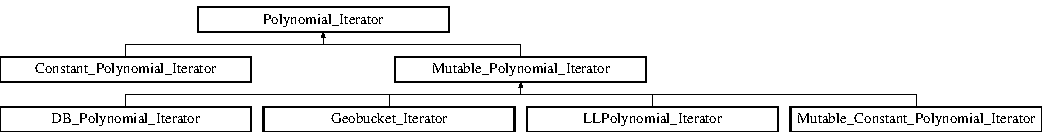
\includegraphics[height=2.000000cm]{group___iterator_group}
\end{center}
\end{figure}
\subsubsection*{Public Member Functions}
\begin{Indent}\textbf{ Construction}\par
\begin{DoxyCompactItemize}
\item 
\hyperlink{group___iterator_group_ab2e59cf23f80448b3b2be7573181c1b7}{Constant\+\_\+\+Polynomial\+\_\+\+Iterator} (const \hyperlink{group__polygroup_class_constant___polynomial}{Constant\+\_\+\+Polynomial} $\ast$q, bool at\+\_\+end=false)
\begin{DoxyCompactList}\small\item\em Creates an iterator for {\ttfamily poly} and starts at the leading term. \end{DoxyCompactList}\end{DoxyCompactItemize}
\end{Indent}
\begin{Indent}\textbf{ Destruction}\par
\begin{DoxyCompactItemize}
\item 
\mbox{\Hypertarget{group___iterator_group_a929c0ee12daaa99dc7961825507434fb}\label{group___iterator_group_a929c0ee12daaa99dc7961825507434fb}} 
{\bfseries $\sim$\+Constant\+\_\+\+Polynomial\+\_\+\+Iterator} ()
\end{DoxyCompactItemize}
\end{Indent}
\begin{Indent}\textbf{ Iteration}\par
\begin{DoxyCompactItemize}
\item 
\mbox{\Hypertarget{group___iterator_group_a897042008adc0e4db52f27616fe30115}\label{group___iterator_group_a897042008adc0e4db52f27616fe30115}} 
virtual void \hyperlink{group___iterator_group_a897042008adc0e4db52f27616fe30115}{restart\+\_\+iteration} () override
\begin{DoxyCompactList}\small\item\em This should move the iterator to the leading term. \end{DoxyCompactList}\item 
\mbox{\Hypertarget{group___iterator_group_a2a9dfd3f6a8520fd3b045f32b12f7ac9}\label{group___iterator_group_a2a9dfd3f6a8520fd3b045f32b12f7ac9}} 
virtual void \hyperlink{group___iterator_group_a2a9dfd3f6a8520fd3b045f32b12f7ac9}{move\+Right} () override
\begin{DoxyCompactList}\small\item\em Moves right in the polynomial, to the next smaller monomial. \end{DoxyCompactList}\item 
\mbox{\Hypertarget{group___iterator_group_ad7ff9576d9d9576acb2776ce42a5dde3}\label{group___iterator_group_ad7ff9576d9d9576acb2776ce42a5dde3}} 
virtual void \hyperlink{group___iterator_group_ad7ff9576d9d9576acb2776ce42a5dde3}{move\+Left} () override
\begin{DoxyCompactList}\small\item\em Moves left in the polynomial, to the next larger monomial. \end{DoxyCompactList}\item 
\mbox{\Hypertarget{group___iterator_group_ad0518860ffbda4026f68495abbaeeba9}\label{group___iterator_group_ad0518860ffbda4026f68495abbaeeba9}} 
virtual bool \hyperlink{group___iterator_group_ad0518860ffbda4026f68495abbaeeba9}{can\+Move\+Right} () const override
\begin{DoxyCompactList}\small\item\em Can this iterator move right, or would it fall off? \end{DoxyCompactList}\item 
virtual bool \hyperlink{group___iterator_group_ade22e36aead8eca568dbd99c6ab73cc2}{can\+Move\+Left} () const override
\item 
virtual bool \hyperlink{group___iterator_group_a1b87a857220a97fe403c5164a51f86eb}{fell\+Off} () const override
\end{DoxyCompactItemize}
\end{Indent}
\begin{Indent}\textbf{ Data access}\par
\begin{DoxyCompactItemize}
\item 
\mbox{\Hypertarget{group___iterator_group_a0c010f1e921bc6180a29bb48abf34888}\label{group___iterator_group_a0c010f1e921bc6180a29bb48abf34888}} 
virtual const \hyperlink{group__polygroup_class_monomial}{Monomial} \& \hyperlink{group___iterator_group_a0c010f1e921bc6180a29bb48abf34888}{curr\+Monomial} () const override
\begin{DoxyCompactList}\small\item\em Reports the monomial at the current position. \end{DoxyCompactList}\item 
\mbox{\Hypertarget{group___iterator_group_a6b26740b4c82a20ebe4dba5226fc0072}\label{group___iterator_group_a6b26740b4c82a20ebe4dba5226fc0072}} 
virtual const \hyperlink{group___fields_group_class_prime___field___element}{Prime\+\_\+\+Field\+\_\+\+Element} \& \hyperlink{group___iterator_group_a6b26740b4c82a20ebe4dba5226fc0072}{curr\+Coeff} () const override
\begin{DoxyCompactList}\small\item\em Reports the coefficient at the current position. \end{DoxyCompactList}\end{DoxyCompactItemize}
\end{Indent}
\subsubsection*{Protected Attributes}
\begin{DoxyCompactItemize}
\item 
\mbox{\Hypertarget{group___iterator_group_ab321ce25d6477f96450100cdc41090a6}\label{group___iterator_group_ab321ce25d6477f96450100cdc41090a6}} 
long \hyperlink{group___iterator_group_ab321ce25d6477f96450100cdc41090a6}{i}
\begin{DoxyCompactList}\small\item\em current position in p's array \end{DoxyCompactList}\item 
\mbox{\Hypertarget{group___iterator_group_a5eb1e51bcc01a9da6dffd950a3e1b1ca}\label{group___iterator_group_a5eb1e51bcc01a9da6dffd950a3e1b1ca}} 
const \hyperlink{group__polygroup_class_constant___polynomial}{Constant\+\_\+\+Polynomial} $\ast$ \hyperlink{group___iterator_group_a5eb1e51bcc01a9da6dffd950a3e1b1ca}{p}
\begin{DoxyCompactList}\small\item\em the polynomial we iterate on \end{DoxyCompactList}\end{DoxyCompactItemize}


\paragraph{Constructor \& Destructor Documentation}
\mbox{\Hypertarget{group___iterator_group_ab2e59cf23f80448b3b2be7573181c1b7}\label{group___iterator_group_ab2e59cf23f80448b3b2be7573181c1b7}} 
\index{Constant\+\_\+\+Polynomial\+\_\+\+Iterator@{Constant\+\_\+\+Polynomial\+\_\+\+Iterator}!Constant\+\_\+\+Polynomial\+\_\+\+Iterator@{Constant\+\_\+\+Polynomial\+\_\+\+Iterator}}
\index{Constant\+\_\+\+Polynomial\+\_\+\+Iterator@{Constant\+\_\+\+Polynomial\+\_\+\+Iterator}!Constant\+\_\+\+Polynomial\+\_\+\+Iterator@{Constant\+\_\+\+Polynomial\+\_\+\+Iterator}}
\subparagraph{\texorpdfstring{Constant\+\_\+\+Polynomial\+\_\+\+Iterator()}{Constant\_Polynomial\_Iterator()}}
{\footnotesize\ttfamily Constant\+\_\+\+Polynomial\+\_\+\+Iterator\+::\+Constant\+\_\+\+Polynomial\+\_\+\+Iterator (\begin{DoxyParamCaption}\item[{const \hyperlink{group__polygroup_class_constant___polynomial}{Constant\+\_\+\+Polynomial} $\ast$}]{q,  }\item[{bool}]{at\+\_\+end = {\ttfamily false} }\end{DoxyParamCaption})}



Creates an iterator for {\ttfamily poly} and starts at the leading term. 


\begin{DoxyParams}{Parameters}
{\em at\+\_\+end} & whether to start at the end of the polynomial \\
\hline
{\em q} & polynomial to iterate over \\
\hline
\end{DoxyParams}


Definition at line 23 of file polynomial\+\_\+array.\+cpp.



\paragraph{Member Function Documentation}
\mbox{\Hypertarget{group___iterator_group_ade22e36aead8eca568dbd99c6ab73cc2}\label{group___iterator_group_ade22e36aead8eca568dbd99c6ab73cc2}} 
\index{Constant\+\_\+\+Polynomial\+\_\+\+Iterator@{Constant\+\_\+\+Polynomial\+\_\+\+Iterator}!can\+Move\+Left@{can\+Move\+Left}}
\index{can\+Move\+Left@{can\+Move\+Left}!Constant\+\_\+\+Polynomial\+\_\+\+Iterator@{Constant\+\_\+\+Polynomial\+\_\+\+Iterator}}
\subparagraph{\texorpdfstring{can\+Move\+Left()}{canMoveLeft()}}
{\footnotesize\ttfamily bool Constant\+\_\+\+Polynomial\+\_\+\+Iterator\+::can\+Move\+Left (\begin{DoxyParamCaption}{ }\end{DoxyParamCaption}) const\hspace{0.3cm}{\ttfamily [override]}, {\ttfamily [virtual]}}

\begin{DoxyReturn}{Returns}
Can this iterator move left, or would it fall off? 
\end{DoxyReturn}


Implements \hyperlink{group___iterator_group_a7ab348897446bc182500f84df8a9e590}{Polynomial\+\_\+\+Iterator}.



Definition at line 49 of file polynomial\+\_\+array.\+cpp.

\mbox{\Hypertarget{group___iterator_group_a1b87a857220a97fe403c5164a51f86eb}\label{group___iterator_group_a1b87a857220a97fe403c5164a51f86eb}} 
\index{Constant\+\_\+\+Polynomial\+\_\+\+Iterator@{Constant\+\_\+\+Polynomial\+\_\+\+Iterator}!fell\+Off@{fell\+Off}}
\index{fell\+Off@{fell\+Off}!Constant\+\_\+\+Polynomial\+\_\+\+Iterator@{Constant\+\_\+\+Polynomial\+\_\+\+Iterator}}
\subparagraph{\texorpdfstring{fell\+Off()}{fellOff()}}
{\footnotesize\ttfamily bool Constant\+\_\+\+Polynomial\+\_\+\+Iterator\+::fell\+Off (\begin{DoxyParamCaption}{ }\end{DoxyParamCaption}) const\hspace{0.3cm}{\ttfamily [override]}, {\ttfamily [virtual]}}

\begin{DoxyReturn}{Returns}
true iff the iterator no longer points to a valid monomial.
\end{DoxyReturn}
This is N\+OT the same as pointing to a monomial with coefficient zero; this is true when the iterator would probably report inaccurate data. 

Implements \hyperlink{group___iterator_group_ac571e120134088d6067718bbad513e2d}{Polynomial\+\_\+\+Iterator}.



Definition at line 51 of file polynomial\+\_\+array.\+cpp.

\index{D\+B\+\_\+\+Polynomial\+\_\+\+Iterator@{D\+B\+\_\+\+Polynomial\+\_\+\+Iterator}}\label{class_d_b___polynomial___iterator}
\Hypertarget{group___iterator_group_class_d_b___polynomial___iterator}
\subsubsection{class D\+B\+\_\+\+Polynomial\+\_\+\+Iterator}
Iterator over double-\/buffered polynomials. 

\begin{DoxyAuthor}{Author}
John Perry 
\end{DoxyAuthor}
\begin{DoxyDate}{Date}
2015 
\end{DoxyDate}


Definition at line 38 of file polynomial\+\_\+double\+\_\+buffered.\+hpp.

Inheritance diagram for D\+B\+\_\+\+Polynomial\+\_\+\+Iterator\+:\begin{figure}[H]
\begin{center}
\leavevmode
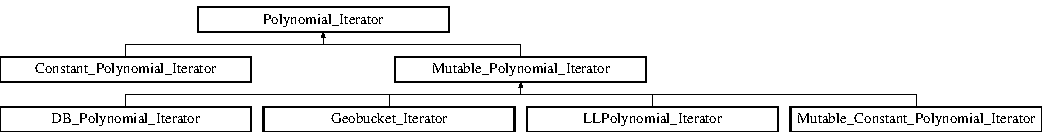
\includegraphics[height=3.000000cm]{group___iterator_group}
\end{center}
\end{figure}
\subsubsection*{Public Member Functions}
\begin{Indent}\textbf{ Construction}\par
\begin{DoxyCompactItemize}
\item 
\mbox{\Hypertarget{group___iterator_group_aa35fe56e92b8c5a866a4f503f3c9a587}\label{group___iterator_group_aa35fe56e92b8c5a866a4f503f3c9a587}} 
{\bfseries D\+B\+\_\+\+Polynomial\+\_\+\+Iterator} (const \hyperlink{group__polygroup_class_double___buffered___polynomial}{Double\+\_\+\+Buffered\+\_\+\+Polynomial} $\ast$f, bool at\+\_\+end=false)
\end{DoxyCompactItemize}
\end{Indent}
\begin{Indent}\textbf{ Destruction}\par
\begin{DoxyCompactItemize}
\item 
\mbox{\Hypertarget{group___iterator_group_af8892a1128109ce22d4b6c57ce5e5398}\label{group___iterator_group_af8892a1128109ce22d4b6c57ce5e5398}} 
{\bfseries $\sim$\+D\+B\+\_\+\+Polynomial\+\_\+\+Iterator} ()
\end{DoxyCompactItemize}
\end{Indent}
\begin{Indent}\textbf{ Iteration}\par
\begin{DoxyCompactItemize}
\item 
\mbox{\Hypertarget{group___iterator_group_a801bfca094868e78f20b94ced6373acc}\label{group___iterator_group_a801bfca094868e78f20b94ced6373acc}} 
virtual void \hyperlink{group___iterator_group_a801bfca094868e78f20b94ced6373acc}{restart\+\_\+iteration} () override
\begin{DoxyCompactList}\small\item\em This should move the iterator to the leading term. \end{DoxyCompactList}\item 
\mbox{\Hypertarget{group___iterator_group_a2617831ba7da31b67993a8c93d2cabbd}\label{group___iterator_group_a2617831ba7da31b67993a8c93d2cabbd}} 
virtual void \hyperlink{group___iterator_group_a2617831ba7da31b67993a8c93d2cabbd}{move\+Right} () override
\begin{DoxyCompactList}\small\item\em Moves right in the polynomial, to the next smaller monomial. \end{DoxyCompactList}\item 
\mbox{\Hypertarget{group___iterator_group_a193d1a443318e64107378c26eff0a876}\label{group___iterator_group_a193d1a443318e64107378c26eff0a876}} 
virtual void \hyperlink{group___iterator_group_a193d1a443318e64107378c26eff0a876}{move\+Left} () override
\begin{DoxyCompactList}\small\item\em Moves left in the polynomial, to the next larger monomial. \end{DoxyCompactList}\item 
virtual bool \hyperlink{group___iterator_group_aa5ee700b0d03a9e333f55a87b2439920}{fell\+Off} () const override
\item 
virtual bool \hyperlink{group___iterator_group_a4094a88fd6d77894ff04960efd492ec6}{can\+Move\+Left} () const override
\item 
\mbox{\Hypertarget{group___iterator_group_a428bdd3ef2ca939404abddd357c4790a}\label{group___iterator_group_a428bdd3ef2ca939404abddd357c4790a}} 
virtual bool \hyperlink{group___iterator_group_a428bdd3ef2ca939404abddd357c4790a}{can\+Move\+Right} () const override
\begin{DoxyCompactList}\small\item\em Can this iterator move right, or would it fall off? \end{DoxyCompactList}\end{DoxyCompactItemize}
\end{Indent}
\begin{Indent}\textbf{ Data access}\par
\begin{DoxyCompactItemize}
\item 
\mbox{\Hypertarget{group___iterator_group_af9b50ef9d8a421be8ca81e1797a4d48e}\label{group___iterator_group_af9b50ef9d8a421be8ca81e1797a4d48e}} 
virtual const \hyperlink{group__polygroup_class_monomial}{Monomial} \& \hyperlink{group___iterator_group_af9b50ef9d8a421be8ca81e1797a4d48e}{curr\+Monomial} () const override
\begin{DoxyCompactList}\small\item\em Reports the monomial at the current position. \end{DoxyCompactList}\item 
\mbox{\Hypertarget{group___iterator_group_ae9458ac44c64c9cb7537dee3b39f66d1}\label{group___iterator_group_ae9458ac44c64c9cb7537dee3b39f66d1}} 
virtual const \hyperlink{group___fields_group_class_prime___field___element}{Prime\+\_\+\+Field\+\_\+\+Element} \& \hyperlink{group___iterator_group_ae9458ac44c64c9cb7537dee3b39f66d1}{curr\+Coeff} () const override
\begin{DoxyCompactList}\small\item\em Reports the coefficient at the current position. \end{DoxyCompactList}\end{DoxyCompactItemize}
\end{Indent}
\begin{Indent}\textbf{ Data modification}\par
\begin{DoxyCompactItemize}
\item 
\mbox{\Hypertarget{group___iterator_group_a2a4349f00960601a5e300fdbd45f6a93}\label{group___iterator_group_a2a4349f00960601a5e300fdbd45f6a93}} 
virtual void \hyperlink{group___iterator_group_a2a4349f00960601a5e300fdbd45f6a93}{set\+\_\+curr\+Coeff} (const \hyperlink{group___fields_group_class_prime___field___element}{Prime\+\_\+\+Field\+\_\+\+Element} \&a) override
\begin{DoxyCompactList}\small\item\em change coefficient in current position \end{DoxyCompactList}\item 
\mbox{\Hypertarget{group___iterator_group_aa5c637091134c2bc47cca2208a43e6e8}\label{group___iterator_group_aa5c637091134c2bc47cca2208a43e6e8}} 
virtual void \hyperlink{group___iterator_group_aa5c637091134c2bc47cca2208a43e6e8}{set\+\_\+curr\+Monomial} (const \hyperlink{group__polygroup_class_monomial}{Monomial} \&t) override
\begin{DoxyCompactList}\small\item\em change monomial in current position \end{DoxyCompactList}\end{DoxyCompactItemize}
\end{Indent}
\subsubsection*{Protected Attributes}
\begin{DoxyCompactItemize}
\item 
\mbox{\Hypertarget{group___iterator_group_a4fef20479db4c9bc1434ddacdbb67590}\label{group___iterator_group_a4fef20479db4c9bc1434ddacdbb67590}} 
\hyperlink{group___fields_group_class_prime___field___element}{Prime\+\_\+\+Field\+\_\+\+Element} $\ast$ \hyperlink{group___iterator_group_a4fef20479db4c9bc1434ddacdbb67590}{A}
\begin{DoxyCompactList}\small\item\em pointer to coefficients \end{DoxyCompactList}\item 
\mbox{\Hypertarget{group___iterator_group_a3f81b1022526da1586eec443e4846ae2}\label{group___iterator_group_a3f81b1022526da1586eec443e4846ae2}} 
long long \hyperlink{group___iterator_group_a3f81b1022526da1586eec443e4846ae2}{current\+\_\+position}
\begin{DoxyCompactList}\small\item\em current position in the list \end{DoxyCompactList}\item 
\mbox{\Hypertarget{group___iterator_group_a6d2f1a91150d12a8835395a678260968}\label{group___iterator_group_a6d2f1a91150d12a8835395a678260968}} 
unsigned \hyperlink{group___iterator_group_a6d2f1a91150d12a8835395a678260968}{head}
\begin{DoxyCompactList}\small\item\em position of first monomial \end{DoxyCompactList}\item 
\mbox{\Hypertarget{group___iterator_group_aba055182673176b6390aecd4a5bb31d4}\label{group___iterator_group_aba055182673176b6390aecd4a5bb31d4}} 
\hyperlink{group__polygroup_class_monomial}{Monomial} $\ast$ \hyperlink{group___iterator_group_aba055182673176b6390aecd4a5bb31d4}{T}
\begin{DoxyCompactList}\small\item\em pointer to monomials \end{DoxyCompactList}\item 
\mbox{\Hypertarget{group___iterator_group_a57a302fde5b37005fc52d8d022d7284f}\label{group___iterator_group_a57a302fde5b37005fc52d8d022d7284f}} 
unsigned \hyperlink{group___iterator_group_a57a302fde5b37005fc52d8d022d7284f}{tail}
\begin{DoxyCompactList}\small\item\em position of last monomial \end{DoxyCompactList}\end{DoxyCompactItemize}


\paragraph{Member Function Documentation}
\mbox{\Hypertarget{group___iterator_group_a4094a88fd6d77894ff04960efd492ec6}\label{group___iterator_group_a4094a88fd6d77894ff04960efd492ec6}} 
\index{D\+B\+\_\+\+Polynomial\+\_\+\+Iterator@{D\+B\+\_\+\+Polynomial\+\_\+\+Iterator}!can\+Move\+Left@{can\+Move\+Left}}
\index{can\+Move\+Left@{can\+Move\+Left}!D\+B\+\_\+\+Polynomial\+\_\+\+Iterator@{D\+B\+\_\+\+Polynomial\+\_\+\+Iterator}}
\subparagraph{\texorpdfstring{can\+Move\+Left()}{canMoveLeft()}}
{\footnotesize\ttfamily bool D\+B\+\_\+\+Polynomial\+\_\+\+Iterator\+::can\+Move\+Left (\begin{DoxyParamCaption}{ }\end{DoxyParamCaption}) const\hspace{0.3cm}{\ttfamily [override]}, {\ttfamily [virtual]}}

\begin{DoxyReturn}{Returns}
Can this iterator move left, or would it fall off? 
\end{DoxyReturn}


Implements \hyperlink{group___iterator_group_a7ab348897446bc182500f84df8a9e590}{Polynomial\+\_\+\+Iterator}.



Definition at line 35 of file polynomial\+\_\+double\+\_\+buffered.\+cpp.

\mbox{\Hypertarget{group___iterator_group_aa5ee700b0d03a9e333f55a87b2439920}\label{group___iterator_group_aa5ee700b0d03a9e333f55a87b2439920}} 
\index{D\+B\+\_\+\+Polynomial\+\_\+\+Iterator@{D\+B\+\_\+\+Polynomial\+\_\+\+Iterator}!fell\+Off@{fell\+Off}}
\index{fell\+Off@{fell\+Off}!D\+B\+\_\+\+Polynomial\+\_\+\+Iterator@{D\+B\+\_\+\+Polynomial\+\_\+\+Iterator}}
\subparagraph{\texorpdfstring{fell\+Off()}{fellOff()}}
{\footnotesize\ttfamily bool D\+B\+\_\+\+Polynomial\+\_\+\+Iterator\+::fell\+Off (\begin{DoxyParamCaption}{ }\end{DoxyParamCaption}) const\hspace{0.3cm}{\ttfamily [override]}, {\ttfamily [virtual]}}

\begin{DoxyReturn}{Returns}
true iff the iterator no longer points to a valid monomial.
\end{DoxyReturn}
This is N\+OT the same as pointing to a monomial with coefficient zero; this is true when the iterator would probably report inaccurate data. 

Implements \hyperlink{group___iterator_group_ac571e120134088d6067718bbad513e2d}{Polynomial\+\_\+\+Iterator}.



Definition at line 31 of file polynomial\+\_\+double\+\_\+buffered.\+cpp.

\index{Geobucket\+\_\+\+Iterator@{Geobucket\+\_\+\+Iterator}}\label{class_geobucket___iterator}
\Hypertarget{group___iterator_group_class_geobucket___iterator}
\subsubsection{class Geobucket\+\_\+\+Iterator}
Iterates through polynomials using a geobucket representation. See \hyperlink{group___iterator_group_class_mutable___polynomial___iterator}{Mutable\+\_\+\+Polynomial\+\_\+\+Iterator} for details on methods. 

\begin{DoxyAuthor}{Author}
John Perry 
\end{DoxyAuthor}
\begin{DoxyDate}{Date}
2015
\end{DoxyDate}
Implementation based on \cite{YanGeobuckets}. \begin{DoxyWarning}{Warning}
A polynomial in geobucket representation may not be fully simplified. Clients must not expect the monomials to be in any sort of order, and multiple instances of a monomial are possible. Geobuckets collapse only at canonicalization. 
\end{DoxyWarning}


Definition at line 58 of file polynomial\+\_\+geobucket.\+hpp.

Inheritance diagram for Geobucket\+\_\+\+Iterator\+:\begin{figure}[H]
\begin{center}
\leavevmode
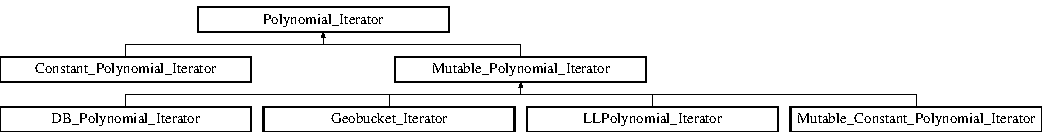
\includegraphics[height=3.000000cm]{group___iterator_group}
\end{center}
\end{figure}
\subsubsection*{Public Member Functions}
\begin{Indent}\textbf{ Construction}\par
\begin{DoxyCompactItemize}
\item 
\mbox{\Hypertarget{group___iterator_group_a1cf41a066244e2f0b6919f8e1b3d799d}\label{group___iterator_group_a1cf41a066244e2f0b6919f8e1b3d799d}} 
{\bfseries Geobucket\+\_\+\+Iterator} (const \hyperlink{group__polygroup_class_polynomial___geobucket}{Polynomial\+\_\+\+Geobucket} $\ast$, bool at\+\_\+end=false)
\item 
\mbox{\Hypertarget{group___iterator_group_a9aef2105e723b8c2d52f5030d437f005}\label{group___iterator_group_a9aef2105e723b8c2d52f5030d437f005}} 
{\bfseries Geobucket\+\_\+\+Iterator} (\hyperlink{group__polygroup_class_polynomial___geobucket}{Polynomial\+\_\+\+Geobucket} $\ast$, bool at\+\_\+end=false)
\end{DoxyCompactItemize}
\end{Indent}
\begin{Indent}\textbf{ Destruction}\par
\begin{DoxyCompactItemize}
\item 
\mbox{\Hypertarget{group___iterator_group_a474cb782876a334af8a4cd6c3f9f989c}\label{group___iterator_group_a474cb782876a334af8a4cd6c3f9f989c}} 
{\bfseries $\sim$\+Geobucket\+\_\+\+Iterator} ()
\end{DoxyCompactItemize}
\end{Indent}
\begin{Indent}\textbf{ Iteration}\par
\begin{DoxyCompactItemize}
\item 
\mbox{\Hypertarget{group___iterator_group_a2acbad922f8fdd33300e49979773ba00}\label{group___iterator_group_a2acbad922f8fdd33300e49979773ba00}} 
virtual void \hyperlink{group___iterator_group_a2acbad922f8fdd33300e49979773ba00}{restart\+\_\+iteration} () override
\begin{DoxyCompactList}\small\item\em This should move the iterator to the leading term. \end{DoxyCompactList}\item 
\mbox{\Hypertarget{group___iterator_group_a1124336f77c6d4dffdc6d3da4d6078ed}\label{group___iterator_group_a1124336f77c6d4dffdc6d3da4d6078ed}} 
virtual void \hyperlink{group___iterator_group_a1124336f77c6d4dffdc6d3da4d6078ed}{move\+Right} () override
\begin{DoxyCompactList}\small\item\em Moves right in the polynomial, to the next smaller monomial. \end{DoxyCompactList}\item 
\mbox{\Hypertarget{group___iterator_group_ae94baa36d6b096c1144068dc21108c23}\label{group___iterator_group_ae94baa36d6b096c1144068dc21108c23}} 
virtual void \hyperlink{group___iterator_group_ae94baa36d6b096c1144068dc21108c23}{move\+Left} () override
\begin{DoxyCompactList}\small\item\em Moves left in the polynomial, to the next larger monomial. \end{DoxyCompactList}\item 
\mbox{\Hypertarget{group___iterator_group_ad24c1412a9027a2d02faf946c8471985}\label{group___iterator_group_ad24c1412a9027a2d02faf946c8471985}} 
virtual bool \hyperlink{group___iterator_group_ad24c1412a9027a2d02faf946c8471985}{can\+Move\+Right} () const override
\begin{DoxyCompactList}\small\item\em Can this iterator move right, or would it fall off? \end{DoxyCompactList}\item 
virtual bool \hyperlink{group___iterator_group_a6c3db5961d5faf1b465c51e8935e0b89}{can\+Move\+Left} () const override
\item 
virtual bool \hyperlink{group___iterator_group_a44ac71c5f71fc2830c74c4d289c9aec8}{fell\+Off} () const override
\end{DoxyCompactItemize}
\end{Indent}
\begin{Indent}\textbf{ Data access}\par
\begin{DoxyCompactItemize}
\item 
\mbox{\Hypertarget{group___iterator_group_a56793799db6e9db7bfc2a85c9d9c6849}\label{group___iterator_group_a56793799db6e9db7bfc2a85c9d9c6849}} 
virtual const \hyperlink{group__polygroup_class_monomial}{Monomial} \& \hyperlink{group___iterator_group_a56793799db6e9db7bfc2a85c9d9c6849}{curr\+Monomial} () const override
\begin{DoxyCompactList}\small\item\em Reports the monomial at the current position. \end{DoxyCompactList}\item 
\mbox{\Hypertarget{group___iterator_group_a9c8021b6917f21f3b240759fd6e31b4e}\label{group___iterator_group_a9c8021b6917f21f3b240759fd6e31b4e}} 
virtual const \hyperlink{group___fields_group_class_prime___field___element}{Prime\+\_\+\+Field\+\_\+\+Element} \& \hyperlink{group___iterator_group_a9c8021b6917f21f3b240759fd6e31b4e}{curr\+Coeff} () const override
\begin{DoxyCompactList}\small\item\em Reports the coefficient at the current position. \end{DoxyCompactList}\end{DoxyCompactItemize}
\end{Indent}
\begin{Indent}\textbf{ Data modification}\par
\begin{DoxyCompactItemize}
\item 
\mbox{\Hypertarget{group___iterator_group_ab425503b966e0d129e55bb44ea84ca5c}\label{group___iterator_group_ab425503b966e0d129e55bb44ea84ca5c}} 
virtual void \hyperlink{group___iterator_group_ab425503b966e0d129e55bb44ea84ca5c}{set\+\_\+curr\+Coeff} (const \hyperlink{group___fields_group_class_prime___field___element}{Prime\+\_\+\+Field\+\_\+\+Element} \&a) override
\begin{DoxyCompactList}\small\item\em change coefficient in current position \end{DoxyCompactList}\item 
\mbox{\Hypertarget{group___iterator_group_adc1c1425e4eba02105c27f9fadc76d7b}\label{group___iterator_group_adc1c1425e4eba02105c27f9fadc76d7b}} 
virtual void \hyperlink{group___iterator_group_adc1c1425e4eba02105c27f9fadc76d7b}{set\+\_\+curr\+Monomial} (const \hyperlink{group__polygroup_class_monomial}{Monomial} \&t) override
\begin{DoxyCompactList}\small\item\em change monomial in current position \end{DoxyCompactList}\end{DoxyCompactItemize}
\end{Indent}
\subsubsection*{Protected Attributes}
\begin{DoxyCompactItemize}
\item 
\mbox{\Hypertarget{group___iterator_group_a3a32af8a6cb4d462a3b325721bd2a11b}\label{group___iterator_group_a3a32af8a6cb4d462a3b325721bd2a11b}} 
unsigned \hyperlink{group___iterator_group_a3a32af8a6cb4d462a3b325721bd2a11b}{bucket\+\_\+number}
\begin{DoxyCompactList}\small\item\em the bucket number at which we're stopped \end{DoxyCompactList}\item 
\mbox{\Hypertarget{group___iterator_group_a17836580130b78ffc1fb62b9bf67c286}\label{group___iterator_group_a17836580130b78ffc1fb62b9bf67c286}} 
\hyperlink{group__polygroup_class_polynomial___geobucket}{Polynomial\+\_\+\+Geobucket} $\ast$ \hyperlink{group___iterator_group_a17836580130b78ffc1fb62b9bf67c286}{g}
\begin{DoxyCompactList}\small\item\em to save myself the hassle of {\ttfamily static\+\_\+cast$<$const Polynomial\+\_\+\+Geobucket $\ast$$>$(p)} every time I turn around \end{DoxyCompactList}\item 
\mbox{\Hypertarget{group___iterator_group_a484bb97ad82643d5b82733f6cbee8e8c}\label{group___iterator_group_a484bb97ad82643d5b82733f6cbee8e8c}} 
\hyperlink{group___iterator_group_class_l_l_polynomial___iterator}{L\+L\+Polynomial\+\_\+\+Iterator} $\ast$ \hyperlink{group___iterator_group_a484bb97ad82643d5b82733f6cbee8e8c}{pi}
\begin{DoxyCompactList}\small\item\em an iterator for the current bucket \end{DoxyCompactList}\end{DoxyCompactItemize}


\paragraph{Member Function Documentation}
\mbox{\Hypertarget{group___iterator_group_a6c3db5961d5faf1b465c51e8935e0b89}\label{group___iterator_group_a6c3db5961d5faf1b465c51e8935e0b89}} 
\index{Geobucket\+\_\+\+Iterator@{Geobucket\+\_\+\+Iterator}!can\+Move\+Left@{can\+Move\+Left}}
\index{can\+Move\+Left@{can\+Move\+Left}!Geobucket\+\_\+\+Iterator@{Geobucket\+\_\+\+Iterator}}
\subparagraph{\texorpdfstring{can\+Move\+Left()}{canMoveLeft()}}
{\footnotesize\ttfamily bool Geobucket\+\_\+\+Iterator\+::can\+Move\+Left (\begin{DoxyParamCaption}{ }\end{DoxyParamCaption}) const\hspace{0.3cm}{\ttfamily [override]}, {\ttfamily [virtual]}}

\begin{DoxyReturn}{Returns}
Can this iterator move left, or would it fall off? 
\end{DoxyReturn}


Implements \hyperlink{group___iterator_group_a7ab348897446bc182500f84df8a9e590}{Polynomial\+\_\+\+Iterator}.



Definition at line 23 of file polynomial\+\_\+geobucket.\+cpp.

\mbox{\Hypertarget{group___iterator_group_a44ac71c5f71fc2830c74c4d289c9aec8}\label{group___iterator_group_a44ac71c5f71fc2830c74c4d289c9aec8}} 
\index{Geobucket\+\_\+\+Iterator@{Geobucket\+\_\+\+Iterator}!fell\+Off@{fell\+Off}}
\index{fell\+Off@{fell\+Off}!Geobucket\+\_\+\+Iterator@{Geobucket\+\_\+\+Iterator}}
\subparagraph{\texorpdfstring{fell\+Off()}{fellOff()}}
{\footnotesize\ttfamily bool Geobucket\+\_\+\+Iterator\+::fell\+Off (\begin{DoxyParamCaption}{ }\end{DoxyParamCaption}) const\hspace{0.3cm}{\ttfamily [override]}, {\ttfamily [virtual]}}

\begin{DoxyReturn}{Returns}
true iff the iterator no longer points to a valid monomial.
\end{DoxyReturn}
This is N\+OT the same as pointing to a monomial with coefficient zero; this is true when the iterator would probably report inaccurate data. 

Implements \hyperlink{group___iterator_group_ac571e120134088d6067718bbad513e2d}{Polynomial\+\_\+\+Iterator}.



Definition at line 31 of file polynomial\+\_\+geobucket.\+cpp.

\index{L\+L\+Polynomial\+\_\+\+Iterator@{L\+L\+Polynomial\+\_\+\+Iterator}}\label{class_l_l_polynomial___iterator}
\Hypertarget{group___iterator_group_class_l_l_polynomial___iterator}
\subsubsection{class L\+L\+Polynomial\+\_\+\+Iterator}
Iterator over linked list polynomials. 

\begin{DoxyAuthor}{Author}
John Perry 
\end{DoxyAuthor}
\begin{DoxyDate}{Date}
2015 
\end{DoxyDate}


Definition at line 102 of file polynomial\+\_\+linked\+\_\+list.\+hpp.

Inheritance diagram for L\+L\+Polynomial\+\_\+\+Iterator\+:\begin{figure}[H]
\begin{center}
\leavevmode
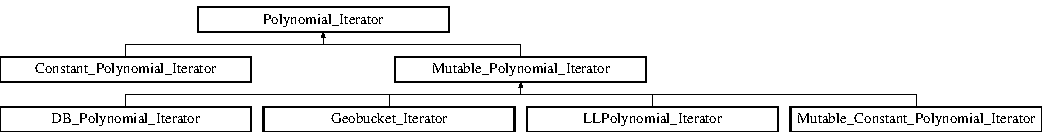
\includegraphics[height=3.000000cm]{group___iterator_group}
\end{center}
\end{figure}
\subsubsection*{Public Member Functions}
\begin{Indent}\textbf{ Construction}\par
\begin{DoxyCompactItemize}
\item 
\mbox{\Hypertarget{group___iterator_group_aef49d7f26dd804b0ab0affbe1567fd07}\label{group___iterator_group_aef49d7f26dd804b0ab0affbe1567fd07}} 
\hyperlink{group___iterator_group_aef49d7f26dd804b0ab0affbe1567fd07}{L\+L\+Polynomial\+\_\+\+Iterator} (\hyperlink{group__polygroup_class_polynomial___linked___list}{Polynomial\+\_\+\+Linked\+\_\+\+List} $\ast$poly, bool at\+\_\+end=false)
\begin{DoxyCompactList}\small\item\em Initializes at the leading monomial. \end{DoxyCompactList}\item 
\mbox{\Hypertarget{group___iterator_group_a957ab5441b10a681f647fe4417b2d373}\label{group___iterator_group_a957ab5441b10a681f647fe4417b2d373}} 
\hyperlink{group___iterator_group_a957ab5441b10a681f647fe4417b2d373}{L\+L\+Polynomial\+\_\+\+Iterator} (const \hyperlink{group__polygroup_class_polynomial___linked___list}{Polynomial\+\_\+\+Linked\+\_\+\+List} $\ast$poly, bool at\+\_\+end=false)
\begin{DoxyCompactList}\small\item\em Initializes at the leading monomial. \end{DoxyCompactList}\end{DoxyCompactItemize}
\end{Indent}
\begin{Indent}\textbf{ Iteration}\par
\begin{DoxyCompactItemize}
\item 
\mbox{\Hypertarget{group___iterator_group_ab369923171f62e5f0cdb83ef7dd6f6e8}\label{group___iterator_group_ab369923171f62e5f0cdb83ef7dd6f6e8}} 
virtual void \hyperlink{group___iterator_group_ab369923171f62e5f0cdb83ef7dd6f6e8}{restart\+\_\+iteration} () override
\begin{DoxyCompactList}\small\item\em Initializes at the leading monomial. \end{DoxyCompactList}\item 
virtual void \hyperlink{group___iterator_group_a2bb830c4e310d91b39e55b05ce86840c}{move\+Right} () override
\begin{DoxyCompactList}\small\item\em Returns the monomial the iterator currently points to. \end{DoxyCompactList}\item 
\mbox{\Hypertarget{group___iterator_group_a5ede434de909b2391d83b3bca4fdc4d7}\label{group___iterator_group_a5ede434de909b2391d83b3bca4fdc4d7}} 
virtual void \hyperlink{group___iterator_group_a5ede434de909b2391d83b3bca4fdc4d7}{move\+Left} () override
\begin{DoxyCompactList}\small\item\em Moves the iterator left\+: to the next larger monomial. \end{DoxyCompactList}\item 
\mbox{\Hypertarget{group___iterator_group_a2df38ef3fd64b5e90432c754ce21f0c4}\label{group___iterator_group_a2df38ef3fd64b5e90432c754ce21f0c4}} 
virtual bool \hyperlink{group___iterator_group_a2df38ef3fd64b5e90432c754ce21f0c4}{can\+Move\+Left} () const override
\begin{DoxyCompactList}\small\item\em Can this iterator move left, or would it fall off? \end{DoxyCompactList}\item 
\mbox{\Hypertarget{group___iterator_group_adbd438dcd2aafa61eb2c07873b90f751}\label{group___iterator_group_adbd438dcd2aafa61eb2c07873b90f751}} 
virtual bool \hyperlink{group___iterator_group_adbd438dcd2aafa61eb2c07873b90f751}{can\+Move\+Right} () const override
\begin{DoxyCompactList}\small\item\em Can this iterator move right, or would it fall off? \end{DoxyCompactList}\item 
\mbox{\Hypertarget{group___iterator_group_ab6471b426bf5645dacd2369c0ab441f5}\label{group___iterator_group_ab6471b426bf5645dacd2369c0ab441f5}} 
virtual bool \hyperlink{group___iterator_group_ab6471b426bf5645dacd2369c0ab441f5}{fell\+Off} () const override
\begin{DoxyCompactList}\small\item\em true iff the iterator no longer points to a valid monomial. \end{DoxyCompactList}\end{DoxyCompactItemize}
\end{Indent}
\begin{Indent}\textbf{ Data access}\par
\begin{DoxyCompactItemize}
\item 
\mbox{\Hypertarget{group___iterator_group_a0a8c14daf501f3ab4a6f708aabf21f08}\label{group___iterator_group_a0a8c14daf501f3ab4a6f708aabf21f08}} 
virtual const \hyperlink{group__polygroup_class_monomial}{Monomial} \& \hyperlink{group___iterator_group_a0a8c14daf501f3ab4a6f708aabf21f08}{curr\+Monomial} () const override
\begin{DoxyCompactList}\small\item\em Reports the monomial at the current position. \end{DoxyCompactList}\item 
\mbox{\Hypertarget{group___iterator_group_a1ae954211a895e0a73ffd51e569161dc}\label{group___iterator_group_a1ae954211a895e0a73ffd51e569161dc}} 
virtual const \hyperlink{group___fields_group_class_prime___field___element}{Prime\+\_\+\+Field\+\_\+\+Element} \& \hyperlink{group___iterator_group_a1ae954211a895e0a73ffd51e569161dc}{curr\+Coeff} () const override
\begin{DoxyCompactList}\small\item\em Returns the coefficient of the monomial the iterator currently points to. \end{DoxyCompactList}\end{DoxyCompactItemize}
\end{Indent}
\subsubsection*{Data modification}
\begin{DoxyCompactItemize}
\item 
\hyperlink{group__polygroup_class_polynomial___linked___list}{Polynomial\+\_\+\+Linked\+\_\+\+List} $\ast$ \hyperlink{group___iterator_group_a50151664e42e30b845a0a0d11577cfff}{p}
\begin{DoxyCompactList}\small\item\em @ \end{DoxyCompactList}\item 
\mbox{\Hypertarget{group___iterator_group_a750f8f8dd1e33b8a7107aa1b717eec72}\label{group___iterator_group_a750f8f8dd1e33b8a7107aa1b717eec72}} 
\hyperlink{group__polygroup_class_monomial___node}{Monomial\+\_\+\+Node} $\ast$ \hyperlink{group___iterator_group_a750f8f8dd1e33b8a7107aa1b717eec72}{iter\+\_\+curr}
\begin{DoxyCompactList}\small\item\em the node at which we have stopped \end{DoxyCompactList}\item 
\mbox{\Hypertarget{group___iterator_group_a4768fb7fbe060737c964e4179e9102c6}\label{group___iterator_group_a4768fb7fbe060737c964e4179e9102c6}} 
virtual void \hyperlink{group___iterator_group_a4768fb7fbe060737c964e4179e9102c6}{set\+\_\+curr\+Coeff} (const \hyperlink{group___fields_group_class_prime___field___element}{Prime\+\_\+\+Field\+\_\+\+Element} \&a) override
\begin{DoxyCompactList}\small\item\em change coefficient in current position \end{DoxyCompactList}\item 
\mbox{\Hypertarget{group___iterator_group_abb1e45baaf38bc96bcae22a512135fda}\label{group___iterator_group_abb1e45baaf38bc96bcae22a512135fda}} 
virtual void \hyperlink{group___iterator_group_abb1e45baaf38bc96bcae22a512135fda}{set\+\_\+curr\+Monomial} (const \hyperlink{group__polygroup_class_monomial}{Monomial} \&t) override
\begin{DoxyCompactList}\small\item\em change monomial in current position \end{DoxyCompactList}\end{DoxyCompactItemize}
\subsection*{Additional Inherited Members}


\paragraph{Member Function Documentation}
\mbox{\Hypertarget{group___iterator_group_a2bb830c4e310d91b39e55b05ce86840c}\label{group___iterator_group_a2bb830c4e310d91b39e55b05ce86840c}} 
\index{L\+L\+Polynomial\+\_\+\+Iterator@{L\+L\+Polynomial\+\_\+\+Iterator}!move\+Right@{move\+Right}}
\index{move\+Right@{move\+Right}!L\+L\+Polynomial\+\_\+\+Iterator@{L\+L\+Polynomial\+\_\+\+Iterator}}
\subparagraph{\texorpdfstring{move\+Right()}{moveRight()}}
{\footnotesize\ttfamily virtual void L\+L\+Polynomial\+\_\+\+Iterator\+::move\+Right (\begin{DoxyParamCaption}{ }\end{DoxyParamCaption})\hspace{0.3cm}{\ttfamily [inline]}, {\ttfamily [override]}, {\ttfamily [virtual]}}



Returns the monomial the iterator currently points to. 

Moves the iterator right\+: to the next smaller monomial. 

Implements \hyperlink{group___iterator_group_ad7adb26df3077c6c7dec39e066436ce9}{Polynomial\+\_\+\+Iterator}.



Definition at line 128 of file polynomial\+\_\+linked\+\_\+list.\+hpp.



\paragraph{Member Data Documentation}
\mbox{\Hypertarget{group___iterator_group_a50151664e42e30b845a0a0d11577cfff}\label{group___iterator_group_a50151664e42e30b845a0a0d11577cfff}} 
\index{L\+L\+Polynomial\+\_\+\+Iterator@{L\+L\+Polynomial\+\_\+\+Iterator}!p@{p}}
\index{p@{p}!L\+L\+Polynomial\+\_\+\+Iterator@{L\+L\+Polynomial\+\_\+\+Iterator}}
\subparagraph{\texorpdfstring{p}{p}}
{\footnotesize\ttfamily \hyperlink{group__polygroup_class_polynomial___linked___list}{Polynomial\+\_\+\+Linked\+\_\+\+List}$\ast$ L\+L\+Polynomial\+\_\+\+Iterator\+::p\hspace{0.3cm}{\ttfamily [protected]}}



@ 

the polynomial over which we iterate 

Definition at line 159 of file polynomial\+\_\+linked\+\_\+list.\+hpp.

\index{Mutable\+\_\+\+Constant\+\_\+\+Polynomial\+\_\+\+Iterator@{Mutable\+\_\+\+Constant\+\_\+\+Polynomial\+\_\+\+Iterator}}\label{class_mutable___constant___polynomial___iterator}
\Hypertarget{group___iterator_group_class_mutable___constant___polynomial___iterator}
\subsubsection{class Mutable\+\_\+\+Constant\+\_\+\+Polynomial\+\_\+\+Iterator}
An iterator to modify monomials and coefficients of a \hyperlink{group__polygroup_class_constant___polynomial}{Constant\+\_\+\+Polynomial}. 

\begin{DoxyAuthor}{Author}
John Perry 
\end{DoxyAuthor}
\begin{DoxyDate}{Date}
2015
\end{DoxyDate}
Sometimes we want to be able to change particular monomials in a \hyperlink{group__polygroup_class_constant___polynomial}{Constant\+\_\+\+Polynomial}. This a bit naughty, since it violates the spirit of a \hyperlink{group__polygroup_class_constant___polynomial}{Constant\+\_\+\+Polynomial}. I guess I need a different name for the latter. This generally mimics a \hyperlink{group___iterator_group_class_constant___polynomial___iterator}{Constant\+\_\+\+Polynomial\+\_\+\+Iterator}, but cannot inherit from it due to issues with the {\ttfamily const} keyword. This may reflect bad design. 

Definition at line 253 of file polynomial\+\_\+array.\+hpp.

Inheritance diagram for Mutable\+\_\+\+Constant\+\_\+\+Polynomial\+\_\+\+Iterator\+:\begin{figure}[H]
\begin{center}
\leavevmode
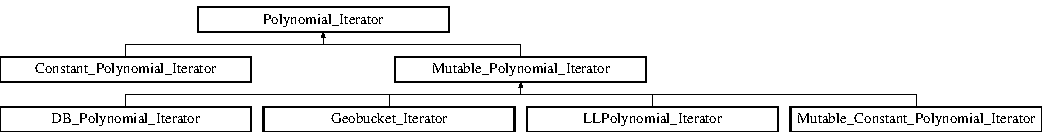
\includegraphics[height=3.000000cm]{group___iterator_group}
\end{center}
\end{figure}
\subsubsection*{Public Member Functions}
\begin{Indent}\textbf{ Construction}\par
\begin{DoxyCompactItemize}
\item 
\hyperlink{group___iterator_group_ac443c5f24675fc7c8fb69bbd167b634b}{Mutable\+\_\+\+Constant\+\_\+\+Polynomial\+\_\+\+Iterator} (\hyperlink{group__polygroup_class_constant___polynomial}{Constant\+\_\+\+Polynomial} $\ast$poly)
\begin{DoxyCompactList}\small\item\em Creates an iterator for {\ttfamily poly} and starts at its leading term. \end{DoxyCompactList}\end{DoxyCompactItemize}
\end{Indent}
\begin{Indent}\textbf{ Destruction}\par
\begin{DoxyCompactItemize}
\item 
\mbox{\Hypertarget{group___iterator_group_a7a4ed35d8a8429bfaf395b034643941b}\label{group___iterator_group_a7a4ed35d8a8429bfaf395b034643941b}} 
{\bfseries $\sim$\+Mutable\+\_\+\+Constant\+\_\+\+Polynomial\+\_\+\+Iterator} ()
\end{DoxyCompactItemize}
\end{Indent}
\begin{Indent}\textbf{ Iteration}\par
\begin{DoxyCompactItemize}
\item 
\mbox{\Hypertarget{group___iterator_group_a039b9076a97e27d93c2393509024c6a3}\label{group___iterator_group_a039b9076a97e27d93c2393509024c6a3}} 
virtual void \hyperlink{group___iterator_group_a039b9076a97e27d93c2393509024c6a3}{restart\+\_\+iteration} () override
\begin{DoxyCompactList}\small\item\em This should move the iterator to the leading term. \end{DoxyCompactList}\item 
\mbox{\Hypertarget{group___iterator_group_ae7570f0ac60c11fe8cddc6ba6e1028a9}\label{group___iterator_group_ae7570f0ac60c11fe8cddc6ba6e1028a9}} 
virtual void \hyperlink{group___iterator_group_ae7570f0ac60c11fe8cddc6ba6e1028a9}{move\+Right} () override
\begin{DoxyCompactList}\small\item\em Moves right in the polynomial, to the next smaller monomial. \end{DoxyCompactList}\item 
\mbox{\Hypertarget{group___iterator_group_a7a2a49f383c6a7c466c107648940bfcf}\label{group___iterator_group_a7a2a49f383c6a7c466c107648940bfcf}} 
virtual void \hyperlink{group___iterator_group_a7a2a49f383c6a7c466c107648940bfcf}{move\+Left} () override
\begin{DoxyCompactList}\small\item\em Moves left in the polynomial, to the next larger monomial. \end{DoxyCompactList}\item 
virtual bool \hyperlink{group___iterator_group_a4c7718296e7be3e5c2b942fa71dd69f2}{fell\+Off} () const override
\end{DoxyCompactItemize}
\end{Indent}
\begin{Indent}\textbf{ Data access}\par
\begin{DoxyCompactItemize}
\item 
\mbox{\Hypertarget{group___iterator_group_a81fa964c3459c2bcefb47e7cd6c8c676}\label{group___iterator_group_a81fa964c3459c2bcefb47e7cd6c8c676}} 
virtual const \hyperlink{group__polygroup_class_monomial}{Monomial} \& \hyperlink{group___iterator_group_a81fa964c3459c2bcefb47e7cd6c8c676}{curr\+Monomial} () const override
\begin{DoxyCompactList}\small\item\em Reports the monomial at the current position. \end{DoxyCompactList}\item 
\mbox{\Hypertarget{group___iterator_group_a5dcae638d3526d75b69fd53c9e50c22d}\label{group___iterator_group_a5dcae638d3526d75b69fd53c9e50c22d}} 
virtual const \hyperlink{group___fields_group_class_prime___field___element}{Prime\+\_\+\+Field\+\_\+\+Element} \& \hyperlink{group___iterator_group_a5dcae638d3526d75b69fd53c9e50c22d}{curr\+Coeff} () const override
\begin{DoxyCompactList}\small\item\em Reports the coefficient at the current position. \end{DoxyCompactList}\end{DoxyCompactItemize}
\end{Indent}
\begin{Indent}\textbf{ Data modification}\par
\begin{DoxyCompactItemize}
\item 
\mbox{\Hypertarget{group___iterator_group_ad5735f8b3c49c632ea7e93956876fed4}\label{group___iterator_group_ad5735f8b3c49c632ea7e93956876fed4}} 
virtual void \hyperlink{group___iterator_group_ad5735f8b3c49c632ea7e93956876fed4}{set\+\_\+curr\+Coeff} (const \hyperlink{group___fields_group_class_prime___field___element}{Prime\+\_\+\+Field\+\_\+\+Element} \&a) override
\begin{DoxyCompactList}\small\item\em change coefficient in current position \end{DoxyCompactList}\item 
\mbox{\Hypertarget{group___iterator_group_aec343a01bd5e134dba01f4acffb0dd45}\label{group___iterator_group_aec343a01bd5e134dba01f4acffb0dd45}} 
virtual void \hyperlink{group___iterator_group_aec343a01bd5e134dba01f4acffb0dd45}{set\+\_\+curr\+Monomial} (const \hyperlink{group__polygroup_class_monomial}{Monomial} \&t) override
\begin{DoxyCompactList}\small\item\em change monomial in current position \end{DoxyCompactList}\end{DoxyCompactItemize}
\end{Indent}
\subsubsection*{Protected Attributes}
\begin{DoxyCompactItemize}
\item 
\mbox{\Hypertarget{group___iterator_group_a7f2a05f25113363d7bb763d579aad653}\label{group___iterator_group_a7f2a05f25113363d7bb763d579aad653}} 
long long \hyperlink{group___iterator_group_a7f2a05f25113363d7bb763d579aad653}{i}
\begin{DoxyCompactList}\small\item\em the monomial we currently point to \end{DoxyCompactList}\item 
\mbox{\Hypertarget{group___iterator_group_a9a9959010a5e8dc6cfdbef7c65ea26da}\label{group___iterator_group_a9a9959010a5e8dc6cfdbef7c65ea26da}} 
\hyperlink{group__polygroup_class_constant___polynomial}{Constant\+\_\+\+Polynomial} $\ast$ \hyperlink{group___iterator_group_a9a9959010a5e8dc6cfdbef7c65ea26da}{p}
\begin{DoxyCompactList}\small\item\em the polynomial over which we iterate \end{DoxyCompactList}\end{DoxyCompactItemize}


\paragraph{Constructor \& Destructor Documentation}
\mbox{\Hypertarget{group___iterator_group_ac443c5f24675fc7c8fb69bbd167b634b}\label{group___iterator_group_ac443c5f24675fc7c8fb69bbd167b634b}} 
\index{Mutable\+\_\+\+Constant\+\_\+\+Polynomial\+\_\+\+Iterator@{Mutable\+\_\+\+Constant\+\_\+\+Polynomial\+\_\+\+Iterator}!Mutable\+\_\+\+Constant\+\_\+\+Polynomial\+\_\+\+Iterator@{Mutable\+\_\+\+Constant\+\_\+\+Polynomial\+\_\+\+Iterator}}
\index{Mutable\+\_\+\+Constant\+\_\+\+Polynomial\+\_\+\+Iterator@{Mutable\+\_\+\+Constant\+\_\+\+Polynomial\+\_\+\+Iterator}!Mutable\+\_\+\+Constant\+\_\+\+Polynomial\+\_\+\+Iterator@{Mutable\+\_\+\+Constant\+\_\+\+Polynomial\+\_\+\+Iterator}}
\subparagraph{\texorpdfstring{Mutable\+\_\+\+Constant\+\_\+\+Polynomial\+\_\+\+Iterator()}{Mutable\_Constant\_Polynomial\_Iterator()}}
{\footnotesize\ttfamily Mutable\+\_\+\+Constant\+\_\+\+Polynomial\+\_\+\+Iterator\+::\+Mutable\+\_\+\+Constant\+\_\+\+Polynomial\+\_\+\+Iterator (\begin{DoxyParamCaption}\item[{\hyperlink{group__polygroup_class_constant___polynomial}{Constant\+\_\+\+Polynomial} $\ast$}]{poly }\end{DoxyParamCaption})}



Creates an iterator for {\ttfamily poly} and starts at its leading term. 


\begin{DoxyParams}{Parameters}
{\em poly} & the polynomial {\ttfamily this} will iterate over \\
\hline
\end{DoxyParams}


Definition at line 267 of file polynomial\+\_\+array.\+cpp.



\paragraph{Member Function Documentation}
\mbox{\Hypertarget{group___iterator_group_a4c7718296e7be3e5c2b942fa71dd69f2}\label{group___iterator_group_a4c7718296e7be3e5c2b942fa71dd69f2}} 
\index{Mutable\+\_\+\+Constant\+\_\+\+Polynomial\+\_\+\+Iterator@{Mutable\+\_\+\+Constant\+\_\+\+Polynomial\+\_\+\+Iterator}!fell\+Off@{fell\+Off}}
\index{fell\+Off@{fell\+Off}!Mutable\+\_\+\+Constant\+\_\+\+Polynomial\+\_\+\+Iterator@{Mutable\+\_\+\+Constant\+\_\+\+Polynomial\+\_\+\+Iterator}}
\subparagraph{\texorpdfstring{fell\+Off()}{fellOff()}}
{\footnotesize\ttfamily bool Mutable\+\_\+\+Constant\+\_\+\+Polynomial\+\_\+\+Iterator\+::fell\+Off (\begin{DoxyParamCaption}{ }\end{DoxyParamCaption}) const\hspace{0.3cm}{\ttfamily [override]}, {\ttfamily [virtual]}}

\begin{DoxyReturn}{Returns}
true iff the iterator no longer points to a valid monomial.
\end{DoxyReturn}
This is N\+OT the same as pointing to a monomial with coefficient zero; this is true when the iterator would probably report inaccurate data. 

Implements \hyperlink{group___iterator_group_ac571e120134088d6067718bbad513e2d}{Polynomial\+\_\+\+Iterator}.



Definition at line 282 of file polynomial\+\_\+array.\+cpp.

\index{Mutable\+\_\+\+Polynomial\+\_\+\+Iterator@{Mutable\+\_\+\+Polynomial\+\_\+\+Iterator}}\label{class_mutable___polynomial___iterator}
\Hypertarget{group___iterator_group_class_mutable___polynomial___iterator}
\subsubsection{class Mutable\+\_\+\+Polynomial\+\_\+\+Iterator}
A \hyperlink{group___iterator_group_class_mutable___polynomial___iterator}{Mutable\+\_\+\+Polynomial\+\_\+\+Iterator} allows one to modify the terms of a polynomial. 

\begin{DoxyAuthor}{Author}
John Perry 
\end{DoxyAuthor}
\begin{DoxyDate}{Date}
2015 
\end{DoxyDate}


Definition at line 283 of file polynomial.\+hpp.

Inheritance diagram for Mutable\+\_\+\+Polynomial\+\_\+\+Iterator\+:\begin{figure}[H]
\begin{center}
\leavevmode
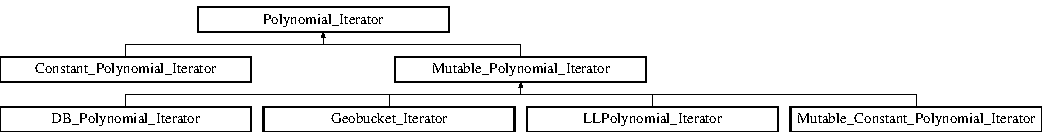
\includegraphics[height=1.779661cm]{group___iterator_group}
\end{center}
\end{figure}
\subsubsection*{Public Member Functions}
\begin{Indent}\textbf{ Data modification}\par
\begin{DoxyCompactItemize}
\item 
\mbox{\Hypertarget{group___iterator_group_a68d273d038b81b687559cf3e7f2c6df3}\label{group___iterator_group_a68d273d038b81b687559cf3e7f2c6df3}} 
virtual void \hyperlink{group___iterator_group_a68d273d038b81b687559cf3e7f2c6df3}{set\+\_\+curr\+Coeff} (const \hyperlink{group___fields_group_class_prime___field___element}{Prime\+\_\+\+Field\+\_\+\+Element} \&)=0
\begin{DoxyCompactList}\small\item\em change coefficient in current position \end{DoxyCompactList}\item 
\mbox{\Hypertarget{group___iterator_group_aeb3668fd81e4284a84c8be4cd2416009}\label{group___iterator_group_aeb3668fd81e4284a84c8be4cd2416009}} 
virtual void \hyperlink{group___iterator_group_aeb3668fd81e4284a84c8be4cd2416009}{set\+\_\+curr\+Monomial} (const \hyperlink{group__polygroup_class_monomial}{Monomial} \&)=0
\begin{DoxyCompactList}\small\item\em change monomial in current position \end{DoxyCompactList}\end{DoxyCompactItemize}
\end{Indent}
\subsection*{Additional Inherited Members}
\index{Polynomial\+\_\+\+Iterator@{Polynomial\+\_\+\+Iterator}}\label{class_polynomial___iterator}
\Hypertarget{group___iterator_group_class_polynomial___iterator}
\subsubsection{class Polynomial\+\_\+\+Iterator}
Used to iterate through a polynomial. 

\begin{DoxyAuthor}{Author}
John Perry 
\end{DoxyAuthor}
\begin{DoxyDate}{Date}
2015
\end{DoxyDate}
This class encapsulates the basic functionality needed to iterate through the monomials of a polynomial. A \hyperlink{group___iterator_group_class_polynomial___iterator}{Polynomial\+\_\+\+Iterator} cannot modify a polynomial, however; to do that, you need a \hyperlink{group___iterator_group_class_mutable___polynomial___iterator}{Mutable\+\_\+\+Polynomial\+\_\+\+Iterator}. 

Definition at line 224 of file polynomial.\+hpp.

Inheritance diagram for Polynomial\+\_\+\+Iterator\+:\begin{figure}[H]
\begin{center}
\leavevmode
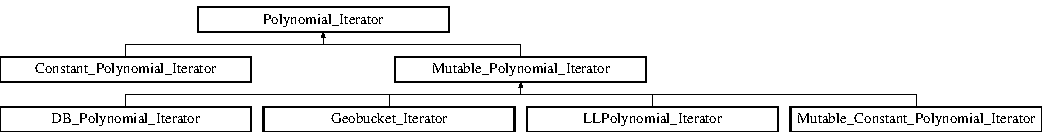
\includegraphics[height=1.779661cm]{group___iterator_group}
\end{center}
\end{figure}
\subsubsection*{Public Member Functions}
\begin{Indent}\textbf{ Destruction}\par
\begin{DoxyCompactItemize}
\item 
\mbox{\Hypertarget{group___iterator_group_a20e700b363cc17d2f8c015f4eca1030f}\label{group___iterator_group_a20e700b363cc17d2f8c015f4eca1030f}} 
virtual \hyperlink{group___iterator_group_a20e700b363cc17d2f8c015f4eca1030f}{$\sim$\+Polynomial\+\_\+\+Iterator} ()=0
\begin{DoxyCompactList}\small\item\em needed to avoid undefined behavior when disposing \end{DoxyCompactList}\end{DoxyCompactItemize}
\end{Indent}
\begin{Indent}\textbf{ Iteration}\par
\begin{DoxyCompactItemize}
\item 
\mbox{\Hypertarget{group___iterator_group_a7135fd6c3a90134741abc2da51467a43}\label{group___iterator_group_a7135fd6c3a90134741abc2da51467a43}} 
virtual void \hyperlink{group___iterator_group_a7135fd6c3a90134741abc2da51467a43}{restart\+\_\+iteration} ()=0
\begin{DoxyCompactList}\small\item\em This should move the iterator to the leading term. \end{DoxyCompactList}\item 
\mbox{\Hypertarget{group___iterator_group_ad7adb26df3077c6c7dec39e066436ce9}\label{group___iterator_group_ad7adb26df3077c6c7dec39e066436ce9}} 
virtual void \hyperlink{group___iterator_group_ad7adb26df3077c6c7dec39e066436ce9}{move\+Right} ()=0
\begin{DoxyCompactList}\small\item\em Moves right in the polynomial, to the next smaller monomial. \end{DoxyCompactList}\item 
\mbox{\Hypertarget{group___iterator_group_a934c291b780f91efefea23880827d5dc}\label{group___iterator_group_a934c291b780f91efefea23880827d5dc}} 
const \hyperlink{group___iterator_group_class_polynomial___iterator}{Polynomial\+\_\+\+Iterator} \& \hyperlink{group___iterator_group_a934c291b780f91efefea23880827d5dc}{operator++} ()
\begin{DoxyCompactList}\small\item\em Moves right in the polynomial, to the next smaller monomial. \end{DoxyCompactList}\item 
\mbox{\Hypertarget{group___iterator_group_ae800f42d78fae005b9d9600b00946026}\label{group___iterator_group_ae800f42d78fae005b9d9600b00946026}} 
virtual bool \hyperlink{group___iterator_group_ae800f42d78fae005b9d9600b00946026}{can\+Move\+Right} () const =0
\begin{DoxyCompactList}\small\item\em Can this iterator move right, or would it fall off? \end{DoxyCompactList}\item 
\mbox{\Hypertarget{group___iterator_group_a47683fc8085c51bd14c5647a7e9e7e87}\label{group___iterator_group_a47683fc8085c51bd14c5647a7e9e7e87}} 
virtual void \hyperlink{group___iterator_group_a47683fc8085c51bd14c5647a7e9e7e87}{move\+Left} ()=0
\begin{DoxyCompactList}\small\item\em Moves left in the polynomial, to the next larger monomial. \end{DoxyCompactList}\item 
virtual bool \hyperlink{group___iterator_group_a7ab348897446bc182500f84df8a9e590}{can\+Move\+Left} () const =0
\item 
virtual bool \hyperlink{group___iterator_group_ac571e120134088d6067718bbad513e2d}{fell\+Off} () const =0
\end{DoxyCompactItemize}
\end{Indent}
\begin{Indent}\textbf{ Data access}\par
\begin{DoxyCompactItemize}
\item 
\mbox{\Hypertarget{group___iterator_group_a7c21bc208d7a71c4a806c4abd1dcf05f}\label{group___iterator_group_a7c21bc208d7a71c4a806c4abd1dcf05f}} 
virtual const \hyperlink{group__polygroup_class_abstract___polynomial}{Abstract\+\_\+\+Polynomial} $\ast$ \hyperlink{group___iterator_group_a7c21bc208d7a71c4a806c4abd1dcf05f}{my\+\_\+poly} () const
\begin{DoxyCompactList}\small\item\em Reports the polynomial on which {\ttfamily this} is iterating. \end{DoxyCompactList}\item 
\mbox{\Hypertarget{group___iterator_group_a95408f0c39ca1cec17dd7802337fe028}\label{group___iterator_group_a95408f0c39ca1cec17dd7802337fe028}} 
virtual const \hyperlink{group__polygroup_class_monomial}{Monomial} \& \hyperlink{group___iterator_group_a95408f0c39ca1cec17dd7802337fe028}{curr\+Monomial} () const =0
\begin{DoxyCompactList}\small\item\em Reports the monomial at the current position. \end{DoxyCompactList}\item 
\mbox{\Hypertarget{group___iterator_group_a92a7e8c4e0054153a2554c8009536405}\label{group___iterator_group_a92a7e8c4e0054153a2554c8009536405}} 
virtual const \hyperlink{group___fields_group_class_prime___field___element}{Prime\+\_\+\+Field\+\_\+\+Element} \& \hyperlink{group___iterator_group_a92a7e8c4e0054153a2554c8009536405}{curr\+Coeff} () const =0
\begin{DoxyCompactList}\small\item\em Reports the coefficient at the current position. \end{DoxyCompactList}\item 
\mbox{\Hypertarget{group___iterator_group_a119cd2937a0cacd43585dee8dc95505f}\label{group___iterator_group_a119cd2937a0cacd43585dee8dc95505f}} 
const \hyperlink{group___iterator_group_class_polynomial___term}{Polynomial\+\_\+\+Term} \hyperlink{group___iterator_group_a119cd2937a0cacd43585dee8dc95505f}{operator$\ast$} () const
\begin{DoxyCompactList}\small\item\em C++11 iteration. \end{DoxyCompactList}\item 
\mbox{\Hypertarget{group___iterator_group_a55bdf643502d14fc6d59df65465d21cd}\label{group___iterator_group_a55bdf643502d14fc6d59df65465d21cd}} 
virtual bool {\bfseries operator!=} (const \hyperlink{group___iterator_group_class_polynomial___iterator}{Polynomial\+\_\+\+Iterator} \&other) const
\end{DoxyCompactItemize}
\end{Indent}
\subsubsection*{Protected Attributes}
\begin{DoxyCompactItemize}
\item 
\mbox{\Hypertarget{group___iterator_group_ab35e9b9c4d7ed12dabce5057a4c2a1b5}\label{group___iterator_group_ab35e9b9c4d7ed12dabce5057a4c2a1b5}} 
const \hyperlink{group__polygroup_class_abstract___polynomial}{Abstract\+\_\+\+Polynomial} $\ast$ \hyperlink{group___iterator_group_ab35e9b9c4d7ed12dabce5057a4c2a1b5}{p}
\begin{DoxyCompactList}\small\item\em the polynomial {\ttfamily this} points to \end{DoxyCompactList}\end{DoxyCompactItemize}


\paragraph{Member Function Documentation}
\mbox{\Hypertarget{group___iterator_group_a7ab348897446bc182500f84df8a9e590}\label{group___iterator_group_a7ab348897446bc182500f84df8a9e590}} 
\index{Polynomial\+\_\+\+Iterator@{Polynomial\+\_\+\+Iterator}!can\+Move\+Left@{can\+Move\+Left}}
\index{can\+Move\+Left@{can\+Move\+Left}!Polynomial\+\_\+\+Iterator@{Polynomial\+\_\+\+Iterator}}
\subparagraph{\texorpdfstring{can\+Move\+Left()}{canMoveLeft()}}
{\footnotesize\ttfamily virtual bool Polynomial\+\_\+\+Iterator\+::can\+Move\+Left (\begin{DoxyParamCaption}{ }\end{DoxyParamCaption}) const\hspace{0.3cm}{\ttfamily [pure virtual]}}

\begin{DoxyReturn}{Returns}
Can this iterator move left, or would it fall off? 
\end{DoxyReturn}


Implemented in \hyperlink{group___iterator_group_a2df38ef3fd64b5e90432c754ce21f0c4}{L\+L\+Polynomial\+\_\+\+Iterator}, \hyperlink{group___iterator_group_a6c3db5961d5faf1b465c51e8935e0b89}{Geobucket\+\_\+\+Iterator}, \hyperlink{group___iterator_group_a4094a88fd6d77894ff04960efd492ec6}{D\+B\+\_\+\+Polynomial\+\_\+\+Iterator}, and \hyperlink{group___iterator_group_ade22e36aead8eca568dbd99c6ab73cc2}{Constant\+\_\+\+Polynomial\+\_\+\+Iterator}.

\mbox{\Hypertarget{group___iterator_group_ac571e120134088d6067718bbad513e2d}\label{group___iterator_group_ac571e120134088d6067718bbad513e2d}} 
\index{Polynomial\+\_\+\+Iterator@{Polynomial\+\_\+\+Iterator}!fell\+Off@{fell\+Off}}
\index{fell\+Off@{fell\+Off}!Polynomial\+\_\+\+Iterator@{Polynomial\+\_\+\+Iterator}}
\subparagraph{\texorpdfstring{fell\+Off()}{fellOff()}}
{\footnotesize\ttfamily virtual bool Polynomial\+\_\+\+Iterator\+::fell\+Off (\begin{DoxyParamCaption}{ }\end{DoxyParamCaption}) const\hspace{0.3cm}{\ttfamily [pure virtual]}}

\begin{DoxyReturn}{Returns}
true iff the iterator no longer points to a valid monomial.
\end{DoxyReturn}
This is N\+OT the same as pointing to a monomial with coefficient zero; this is true when the iterator would probably report inaccurate data. 

Implemented in \hyperlink{group___iterator_group_a4c7718296e7be3e5c2b942fa71dd69f2}{Mutable\+\_\+\+Constant\+\_\+\+Polynomial\+\_\+\+Iterator}, \hyperlink{group___iterator_group_ab6471b426bf5645dacd2369c0ab441f5}{L\+L\+Polynomial\+\_\+\+Iterator}, \hyperlink{group___iterator_group_a44ac71c5f71fc2830c74c4d289c9aec8}{Geobucket\+\_\+\+Iterator}, \hyperlink{group___iterator_group_a1b87a857220a97fe403c5164a51f86eb}{Constant\+\_\+\+Polynomial\+\_\+\+Iterator}, and \hyperlink{group___iterator_group_aa5ee700b0d03a9e333f55a87b2439920}{D\+B\+\_\+\+Polynomial\+\_\+\+Iterator}.

\index{Polynomial\+\_\+\+Term@{Polynomial\+\_\+\+Term}}\label{class_polynomial___term}
\Hypertarget{group___iterator_group_class_polynomial___term}
\subsubsection{class Polynomial\+\_\+\+Term}
convenience class to help iterate through polynomials 

\begin{DoxyAuthor}{Author}
John Perry 
\end{DoxyAuthor}
\begin{DoxyDate}{Date}
2016 
\end{DoxyDate}


Definition at line 60 of file polynomial.\+hpp.

\subsubsection*{Public Member Functions}
\begin{Indent}\textbf{ Construction}\par
\begin{DoxyCompactItemize}
\item 
\mbox{\Hypertarget{group___iterator_group_a62dc1c5f38a989c0bfe40520ebc76d74}\label{group___iterator_group_a62dc1c5f38a989c0bfe40520ebc76d74}} 
{\bfseries Polynomial\+\_\+\+Term} (const \hyperlink{group__polygroup_class_monomial}{Monomial} \&m, const \hyperlink{group___fields_group_class_prime___field___element}{Prime\+\_\+\+Field\+\_\+\+Element} \&a)
\end{DoxyCompactItemize}
\end{Indent}
\begin{Indent}\textbf{ Basic properties}\par
\begin{DoxyCompactItemize}
\item 
\mbox{\Hypertarget{group___iterator_group_aeca1117b51f1326a8c4db38837c84f61}\label{group___iterator_group_aeca1117b51f1326a8c4db38837c84f61}} 
const \hyperlink{group__polygroup_class_monomial}{Monomial} \& \hyperlink{group___iterator_group_aeca1117b51f1326a8c4db38837c84f61}{monomial} ()
\begin{DoxyCompactList}\small\item\em the monomial of this term \end{DoxyCompactList}\item 
\mbox{\Hypertarget{group___iterator_group_afc61ecc1cd633fd0f758bace614711d1}\label{group___iterator_group_afc61ecc1cd633fd0f758bace614711d1}} 
const \hyperlink{group___fields_group_class_prime___field___element}{Prime\+\_\+\+Field\+\_\+\+Element} \& \hyperlink{group___iterator_group_afc61ecc1cd633fd0f758bace614711d1}{coefficient} ()
\begin{DoxyCompactList}\small\item\em the coefficient for this term \end{DoxyCompactList}\end{DoxyCompactItemize}
\end{Indent}
\subsubsection*{Protected Attributes}
\begin{DoxyCompactItemize}
\item 
\mbox{\Hypertarget{group___iterator_group_aacc7304520c8664217e7ce403a82d280}\label{group___iterator_group_aacc7304520c8664217e7ce403a82d280}} 
const \hyperlink{group___fields_group_class_prime___field___element}{Prime\+\_\+\+Field\+\_\+\+Element} \& \hyperlink{group___iterator_group_aacc7304520c8664217e7ce403a82d280}{c}
\begin{DoxyCompactList}\small\item\em the coefficient of this term \end{DoxyCompactList}\item 
\mbox{\Hypertarget{group___iterator_group_a39c6314ec57dce98f2208d02d78e3402}\label{group___iterator_group_a39c6314ec57dce98f2208d02d78e3402}} 
const \hyperlink{group__polygroup_class_monomial}{Monomial} \& \hyperlink{group___iterator_group_a39c6314ec57dce98f2208d02d78e3402}{t}
\begin{DoxyCompactList}\small\item\em the monomial part of this term \end{DoxyCompactList}\end{DoxyCompactItemize}

\hypertarget{group__memorygroup}{}\section{Memory Management}
\label{group__memorygroup}\index{Memory Management@{Memory Management}}


Classes and other structures related to memory management.  


\subsection*{Classes}
\begin{DoxyCompactItemize}
\item 
union \hyperlink{group__memorygroup_uniongoda__block}{goda\+\_\+block$<$ T\+Y\+P\+E $>$}
\begin{DoxyCompactList}\small\item\em heart of the memory pool allocator (\hyperlink{group__memorygroup_class_grading___order___data___allocator}{Grading\+\_\+\+Order\+\_\+\+Data\+\_\+\+Allocator})  \hyperlink{group__memorygroup_uniongoda__block}{More...}\end{DoxyCompactList}\item 
class \hyperlink{group__memorygroup_class_grading___order___data___allocator}{Grading\+\_\+\+Order\+\_\+\+Data\+\_\+\+Allocator$<$ T\+Y\+P\+E $>$}
\begin{DoxyCompactList}\small\item\em special memory pool allocator for \hyperlink{group__orderinggroup_class_grevlex___order___data}{Grevlex\+\_\+\+Order\+\_\+\+Data} and \hyperlink{group__orderinggroup_class_w_grevlex___order___data}{W\+Grevlex\+\_\+\+Order\+\_\+\+Data}  \hyperlink{group__memorygroup_class_grading___order___data___allocator}{More...}\end{DoxyCompactList}\end{DoxyCompactItemize}
\subsection*{Variables}
\begin{DoxyCompactItemize}
\item 
\hyperlink{group__memorygroup_class_grading___order___data___allocator}{Grading\+\_\+\+Order\+\_\+\+Data\+\_\+\+Allocator}$<$ D\+E\+G\+\_\+\+T\+Y\+PE $>$ $\ast$ \hyperlink{group__memorygroup_ga0dc763860167cb9a6e5c84bfda9a456e}{L\+P\+\_\+\+Solvers\+::doda} = nullptr
\begin{DoxyCompactList}\small\item\em memory manager for ray entries \end{DoxyCompactList}\item 
\hyperlink{group__memorygroup_class_grading___order___data___allocator}{Grading\+\_\+\+Order\+\_\+\+Data\+\_\+\+Allocator}$<$ W\+T\+\_\+\+T\+Y\+PE $>$ $\ast$ \hyperlink{group__memorygroup_gadf1bccf09eada41d10a5d4ceda7ca479}{goda} = nullptr
\begin{DoxyCompactList}\small\item\em Memory manager for graded ordering data. \end{DoxyCompactList}\item 
\hyperlink{group__memorygroup_class_grading___order___data___allocator}{Grading\+\_\+\+Order\+\_\+\+Data\+\_\+\+Allocator}$<$ E\+X\+P\+\_\+\+T\+Y\+PE $>$ $\ast$ \hyperlink{group__memorygroup_gaf2c367d23e09c5dad7e0273995a3304c}{moda} = nullptr
\begin{DoxyCompactList}\small\item\em memory manager for monomial exponents \end{DoxyCompactList}\item 
\hyperlink{group__memorygroup_class_grading___order___data___allocator}{Grading\+\_\+\+Order\+\_\+\+Data\+\_\+\+Allocator}$<$ \hyperlink{group__polygroup_class_monomial}{Monomial} $>$ $\ast$ \hyperlink{group__memorygroup_ga76b5ae808895658b417e3f3a13c60e51}{monoda} = nullptr
\begin{DoxyCompactList}\small\item\em memory manager for monomials (not their exponents; see moda for that). \end{DoxyCompactList}\item 
\hyperlink{group__memorygroup_class_grading___order___data___allocator}{Grading\+\_\+\+Order\+\_\+\+Data\+\_\+\+Allocator}$<$ \hyperlink{group__polygroup_class_monomial___node}{Monomial\+\_\+\+Node} $>$ $\ast$ \hyperlink{group__memorygroup_ga2b5eeb775f6c601e624b487f3245983a}{monododa} = nullptr
\begin{DoxyCompactList}\small\item\em memory manager for \hyperlink{group__polygroup_class_monomial___node}{Monomial\+\_\+\+Node} \end{DoxyCompactList}\item 
\hyperlink{group__memorygroup_class_grading___order___data___allocator}{Grading\+\_\+\+Order\+\_\+\+Data\+\_\+\+Allocator}$<$ \hyperlink{group__orderinggroup_class_w_grevlex___order___data}{W\+Grevlex\+\_\+\+Order\+\_\+\+Data} $>$ $\ast$ \hyperlink{group__memorygroup_ga929e61b883d430fc6909a80fdb9ebb83}{woda} = nullptr
\begin{DoxyCompactList}\small\item\em Memory manager for graded orderings (not their data; see goda for that). \end{DoxyCompactList}\end{DoxyCompactItemize}


\subsection{Detailed Description}
Classes and other structures related to memory management. 

These classes create memory pools that allocate large blocks of memory, each of which contains an enormous number of subblocks that can be obtained and released in $O(1)$ time (or at least much more efficiently than {\ttfamily new()} and {\ttfamily delete()}). 

\subsection{Class Documentation}
\index{goda\+\_\+block@{goda\+\_\+block}}\label{uniongoda__block}
\Hypertarget{group__memorygroup_uniongoda__block}
\subsubsection{union goda\+\_\+block}
\subsubsection*{template$<$typename T\+Y\+PE$>$\newline
union goda\+\_\+block$<$ T\+Y\+P\+E $>$}

heart of the memory pool allocator (\hyperlink{group__memorygroup_class_grading___order___data___allocator}{Grading\+\_\+\+Order\+\_\+\+Data\+\_\+\+Allocator}) 

\begin{DoxyAuthor}{Author}
John Perry 
\end{DoxyAuthor}
\begin{DoxyDate}{Date}
2016 
\end{DoxyDate}


Definition at line 45 of file goda.\+hpp.

\begin{DoxyFields}{Class Members}
\mbox{\Hypertarget{group__memorygroup_ad5bea3a00bf688f2db31ad5db90e3deb}\label{group__memorygroup_ad5bea3a00bf688f2db31ad5db90e3deb}} 
TYPE $\ast$&
data&
the data contained in this block \\
\hline

\mbox{\Hypertarget{group__memorygroup_a1f5592b3fed7857bf9336a8e4fba4fdc}\label{group__memorygroup_a1f5592b3fed7857bf9336a8e4fba4fdc}} 
\hyperlink{group__memorygroup_uniongoda__block}{goda\_block} $\ast$&
next&
pointer to the next free block \\
\hline

\end{DoxyFields}
\index{Grading\+\_\+\+Order\+\_\+\+Data\+\_\+\+Allocator@{Grading\+\_\+\+Order\+\_\+\+Data\+\_\+\+Allocator}}\label{class_grading___order___data___allocator}
\Hypertarget{group__memorygroup_class_grading___order___data___allocator}
\subsubsection{class Grading\+\_\+\+Order\+\_\+\+Data\+\_\+\+Allocator}
\subsubsection*{template$<$typename T\+Y\+PE$>$\newline
class Grading\+\_\+\+Order\+\_\+\+Data\+\_\+\+Allocator$<$ T\+Y\+P\+E $>$}

special memory pool allocator for \hyperlink{group__orderinggroup_class_grevlex___order___data}{Grevlex\+\_\+\+Order\+\_\+\+Data} and \hyperlink{group__orderinggroup_class_w_grevlex___order___data}{W\+Grevlex\+\_\+\+Order\+\_\+\+Data} 

\begin{DoxyAuthor}{Author}
John Perry 
\end{DoxyAuthor}
\begin{DoxyDate}{Date}
2016
\end{DoxyDate}
This is a quick-\/n-\/dirty memory pool allocator for \hyperlink{group__orderinggroup_class_grevlex___order___data}{Grevlex\+\_\+\+Order\+\_\+\+Data} and \hyperlink{group__orderinggroup_class_w_grevlex___order___data}{W\+Grevlex\+\_\+\+Order\+\_\+\+Data}. It isn\textquotesingle{}t quite $O(1)$ but the plan is to fix that eventually (I have to locate my notes from class). \begin{DoxyWarning}{Warning}
This is initialized to a certain number of variables, which cannot change. If you want to do this for a different number of variables, create another allocator. 
\end{DoxyWarning}
\begin{Desc}
\item[Examples\+: ]\par
\hyperlink{test_dynamic_8cpp-example}{test\+\_\+dynamic.\+cpp}.\end{Desc}


Definition at line 67 of file goda.\+hpp.

\subsubsection*{Public Member Functions}
\begin{DoxyCompactItemize}
\item 
\hyperlink{group__memorygroup_aa9d14580ced0d2e3d9f0a94e8e83aa85}{Grading\+\_\+\+Order\+\_\+\+Data\+\_\+\+Allocator} (N\+V\+A\+R\+\_\+\+T\+Y\+PE n)
\begin{DoxyCompactList}\small\item\em sets allocator up for blocks of $n$ of type {\ttfamily T\+Y\+PE}. \end{DoxyCompactList}\item 
\mbox{\Hypertarget{group__memorygroup_a01de71b688612c55185fc1fb7fd531b9}\label{group__memorygroup_a01de71b688612c55185fc1fb7fd531b9}} 
\hyperlink{group__memorygroup_a01de71b688612c55185fc1fb7fd531b9}{$\sim$\+Grading\+\_\+\+Order\+\_\+\+Data\+\_\+\+Allocator} ()
\begin{DoxyCompactList}\small\item\em releases all memory --- you\textquotesingle{}d better have freed yours! \end{DoxyCompactList}\item 
\hyperlink{group__memorygroup_uniongoda__block}{goda\+\_\+block}$<$ T\+Y\+PE $>$ $\ast$ \hyperlink{group__memorygroup_a3ac79e785e392024b24c18d60ff3fc3c}{allocate\+\_\+new\+\_\+block} ()
\begin{DoxyCompactList}\small\item\em allocates a new superblock of almost 10000 blocks \end{DoxyCompactList}\item 
T\+Y\+PE $\ast$ \hyperlink{group__memorygroup_a699e85282a021fd7b06f65b9e773eb30}{get\+\_\+new\+\_\+block} ()
\begin{DoxyCompactList}\small\item\em allocates and returns a block of memory \end{DoxyCompactList}\item 
void \hyperlink{group__memorygroup_a518a8f61da93ea93651f426e12761a07}{return\+\_\+used\+\_\+block} (T\+Y\+PE $\ast$freed\+\_\+block)
\begin{DoxyCompactList}\small\item\em returns a block of memory that is no longer needed to the pool \end{DoxyCompactList}\end{DoxyCompactItemize}
\subsubsection*{Protected Attributes}
\begin{DoxyCompactItemize}
\item 
\mbox{\Hypertarget{group__memorygroup_a4c411227a9a3646010a1f22840094c21}\label{group__memorygroup_a4c411227a9a3646010a1f22840094c21}} 
\hyperlink{group__memorygroup_uniongoda__block}{goda\+\_\+block}$<$ T\+Y\+PE $>$ $\ast$ \hyperlink{group__memorygroup_a4c411227a9a3646010a1f22840094c21}{big\+\_\+blocks}
\begin{DoxyCompactList}\small\item\em pointer to the superblock of all blocks \end{DoxyCompactList}\item 
\mbox{\Hypertarget{group__memorygroup_a15e185c6ba2c5262bc03ad13e2dbc223}\label{group__memorygroup_a15e185c6ba2c5262bc03ad13e2dbc223}} 
\hyperlink{group__memorygroup_uniongoda__block}{goda\+\_\+block}$<$ T\+Y\+PE $>$ $\ast$ \hyperlink{group__memorygroup_a15e185c6ba2c5262bc03ad13e2dbc223}{block}
\begin{DoxyCompactList}\small\item\em pointer to the next free block \end{DoxyCompactList}\item 
\mbox{\Hypertarget{group__memorygroup_a7073b652fe474ccd684c1eebd2129a0b}\label{group__memorygroup_a7073b652fe474ccd684c1eebd2129a0b}} 
const unsigned \hyperlink{group__memorygroup_a7073b652fe474ccd684c1eebd2129a0b}{data\+\_\+size}
\begin{DoxyCompactList}\small\item\em how many words to step from one block to the next \end{DoxyCompactList}\end{DoxyCompactItemize}


\paragraph{Constructor \& Destructor Documentation}
\mbox{\Hypertarget{group__memorygroup_aa9d14580ced0d2e3d9f0a94e8e83aa85}\label{group__memorygroup_aa9d14580ced0d2e3d9f0a94e8e83aa85}} 
\index{Grading\+\_\+\+Order\+\_\+\+Data\+\_\+\+Allocator@{Grading\+\_\+\+Order\+\_\+\+Data\+\_\+\+Allocator}!Grading\+\_\+\+Order\+\_\+\+Data\+\_\+\+Allocator@{Grading\+\_\+\+Order\+\_\+\+Data\+\_\+\+Allocator}}
\index{Grading\+\_\+\+Order\+\_\+\+Data\+\_\+\+Allocator@{Grading\+\_\+\+Order\+\_\+\+Data\+\_\+\+Allocator}!Grading\+\_\+\+Order\+\_\+\+Data\+\_\+\+Allocator@{Grading\+\_\+\+Order\+\_\+\+Data\+\_\+\+Allocator}}
\subparagraph{\texorpdfstring{Grading\+\_\+\+Order\+\_\+\+Data\+\_\+\+Allocator()}{Grading\_Order\_Data\_Allocator()}}
{\footnotesize\ttfamily template$<$typename T\+Y\+PE$>$ \\
\hyperlink{group__memorygroup_class_grading___order___data___allocator}{Grading\+\_\+\+Order\+\_\+\+Data\+\_\+\+Allocator}$<$ T\+Y\+PE $>$\+::\hyperlink{group__memorygroup_class_grading___order___data___allocator}{Grading\+\_\+\+Order\+\_\+\+Data\+\_\+\+Allocator} (\begin{DoxyParamCaption}\item[{N\+V\+A\+R\+\_\+\+T\+Y\+PE}]{n }\end{DoxyParamCaption})\hspace{0.3cm}{\ttfamily [inline]}}



sets allocator up for blocks of $n$ of type {\ttfamily T\+Y\+PE}. 


\begin{DoxyParams}{Parameters}
{\em n} & number of objects of type {\ttfamily T\+Y\+PE} that should be allocated initially\\
\hline
\end{DoxyParams}
The \hyperlink{group__memorygroup_class_grading___order___data___allocator}{Grading\+\_\+\+Order\+\_\+\+Data\+\_\+\+Allocator} can and will allocate new blocks of {\ttfamily n} objects when it runs out of room. 

Definition at line 90 of file goda.\+hpp.



\paragraph{Member Function Documentation}
\mbox{\Hypertarget{group__memorygroup_a3ac79e785e392024b24c18d60ff3fc3c}\label{group__memorygroup_a3ac79e785e392024b24c18d60ff3fc3c}} 
\index{Grading\+\_\+\+Order\+\_\+\+Data\+\_\+\+Allocator@{Grading\+\_\+\+Order\+\_\+\+Data\+\_\+\+Allocator}!allocate\+\_\+new\+\_\+block@{allocate\+\_\+new\+\_\+block}}
\index{allocate\+\_\+new\+\_\+block@{allocate\+\_\+new\+\_\+block}!Grading\+\_\+\+Order\+\_\+\+Data\+\_\+\+Allocator@{Grading\+\_\+\+Order\+\_\+\+Data\+\_\+\+Allocator}}
\subparagraph{\texorpdfstring{allocate\+\_\+new\+\_\+block()}{allocate\_new\_block()}}
{\footnotesize\ttfamily template$<$typename T\+Y\+PE$>$ \\
\hyperlink{group__memorygroup_uniongoda__block}{goda\+\_\+block}$<$T\+Y\+PE$>$$\ast$ \hyperlink{group__memorygroup_class_grading___order___data___allocator}{Grading\+\_\+\+Order\+\_\+\+Data\+\_\+\+Allocator}$<$ T\+Y\+PE $>$\+::allocate\+\_\+new\+\_\+block (\begin{DoxyParamCaption}{ }\end{DoxyParamCaption})\hspace{0.3cm}{\ttfamily [inline]}}



allocates a new superblock of almost 10000 blocks 

\begin{DoxyReturn}{Returns}
the superblock 
\end{DoxyReturn}


Definition at line 73 of file goda.\+hpp.

\mbox{\Hypertarget{group__memorygroup_a699e85282a021fd7b06f65b9e773eb30}\label{group__memorygroup_a699e85282a021fd7b06f65b9e773eb30}} 
\index{Grading\+\_\+\+Order\+\_\+\+Data\+\_\+\+Allocator@{Grading\+\_\+\+Order\+\_\+\+Data\+\_\+\+Allocator}!get\+\_\+new\+\_\+block@{get\+\_\+new\+\_\+block}}
\index{get\+\_\+new\+\_\+block@{get\+\_\+new\+\_\+block}!Grading\+\_\+\+Order\+\_\+\+Data\+\_\+\+Allocator@{Grading\+\_\+\+Order\+\_\+\+Data\+\_\+\+Allocator}}
\subparagraph{\texorpdfstring{get\+\_\+new\+\_\+block()}{get\_new\_block()}}
{\footnotesize\ttfamily template$<$typename T\+Y\+PE$>$ \\
T\+Y\+PE$\ast$ \hyperlink{group__memorygroup_class_grading___order___data___allocator}{Grading\+\_\+\+Order\+\_\+\+Data\+\_\+\+Allocator}$<$ T\+Y\+PE $>$\+::get\+\_\+new\+\_\+block (\begin{DoxyParamCaption}{ }\end{DoxyParamCaption})\hspace{0.3cm}{\ttfamily [inline]}}



allocates and returns a block of memory 

\begin{DoxyReturn}{Returns}
block of memory of the size specified in constructor 
\end{DoxyReturn}


Definition at line 108 of file goda.\+hpp.

\mbox{\Hypertarget{group__memorygroup_a518a8f61da93ea93651f426e12761a07}\label{group__memorygroup_a518a8f61da93ea93651f426e12761a07}} 
\index{Grading\+\_\+\+Order\+\_\+\+Data\+\_\+\+Allocator@{Grading\+\_\+\+Order\+\_\+\+Data\+\_\+\+Allocator}!return\+\_\+used\+\_\+block@{return\+\_\+used\+\_\+block}}
\index{return\+\_\+used\+\_\+block@{return\+\_\+used\+\_\+block}!Grading\+\_\+\+Order\+\_\+\+Data\+\_\+\+Allocator@{Grading\+\_\+\+Order\+\_\+\+Data\+\_\+\+Allocator}}
\subparagraph{\texorpdfstring{return\+\_\+used\+\_\+block()}{return\_used\_block()}}
{\footnotesize\ttfamily template$<$typename T\+Y\+PE$>$ \\
void \hyperlink{group__memorygroup_class_grading___order___data___allocator}{Grading\+\_\+\+Order\+\_\+\+Data\+\_\+\+Allocator}$<$ T\+Y\+PE $>$\+::return\+\_\+used\+\_\+block (\begin{DoxyParamCaption}\item[{T\+Y\+PE $\ast$}]{freed\+\_\+block }\end{DoxyParamCaption})\hspace{0.3cm}{\ttfamily [inline]}}



returns a block of memory that is no longer needed to the pool 


\begin{DoxyParams}{Parameters}
{\em freed\+\_\+block} & block to return to the pool \\
\hline
\end{DoxyParams}


Definition at line 121 of file goda.\+hpp.



\subsection{Variable Documentation}
\mbox{\Hypertarget{group__memorygroup_ga0dc763860167cb9a6e5c84bfda9a456e}\label{group__memorygroup_ga0dc763860167cb9a6e5c84bfda9a456e}} 
\index{Memory Management@{Memory Management}!doda@{doda}}
\index{doda@{doda}!Memory Management@{Memory Management}}
\subsubsection{\texorpdfstring{doda}{doda}}
{\footnotesize\ttfamily \hyperlink{group__memorygroup_class_grading___order___data___allocator}{Grading\+\_\+\+Order\+\_\+\+Data\+\_\+\+Allocator}$<$ D\+E\+G\+\_\+\+T\+Y\+PE $>$ $\ast$ L\+P\+\_\+\+Solvers\+::doda = nullptr}



memory manager for ray entries 

Automatically initialized, but clients need to call the destructor when finished. \begin{Desc}
\item[Examples\+: ]\par
\hyperlink{test_dynamic_8cpp-example}{test\+\_\+dynamic.\+cpp}.\end{Desc}


Definition at line 118 of file lp\+\_\+solver.\+cpp.

\mbox{\Hypertarget{group__memorygroup_gadf1bccf09eada41d10a5d4ceda7ca479}\label{group__memorygroup_gadf1bccf09eada41d10a5d4ceda7ca479}} 
\index{Memory Management@{Memory Management}!goda@{goda}}
\index{goda@{goda}!Memory Management@{Memory Management}}
\subsubsection{\texorpdfstring{goda}{goda}}
{\footnotesize\ttfamily \hyperlink{group__memorygroup_class_grading___order___data___allocator}{Grading\+\_\+\+Order\+\_\+\+Data\+\_\+\+Allocator}$<$W\+T\+\_\+\+T\+Y\+PE$>$$\ast$ goda = nullptr}



Memory manager for graded ordering data. 

Automatically initialized, but clients need to call the destructor when finished. 

Definition at line 34 of file particular\+\_\+orderings.\+cpp.

\mbox{\Hypertarget{group__memorygroup_gaf2c367d23e09c5dad7e0273995a3304c}\label{group__memorygroup_gaf2c367d23e09c5dad7e0273995a3304c}} 
\index{Memory Management@{Memory Management}!moda@{moda}}
\index{moda@{moda}!Memory Management@{Memory Management}}
\subsubsection{\texorpdfstring{moda}{moda}}
{\footnotesize\ttfamily \hyperlink{group__memorygroup_class_grading___order___data___allocator}{Grading\+\_\+\+Order\+\_\+\+Data\+\_\+\+Allocator}$<$E\+X\+P\+\_\+\+T\+Y\+PE$>$$\ast$ moda = nullptr}



memory manager for monomial exponents 

Automatically initialized, but clients need to call the destructor when finished. 

Definition at line 48 of file monomial.\+cpp.

\mbox{\Hypertarget{group__memorygroup_ga76b5ae808895658b417e3f3a13c60e51}\label{group__memorygroup_ga76b5ae808895658b417e3f3a13c60e51}} 
\index{Memory Management@{Memory Management}!monoda@{monoda}}
\index{monoda@{monoda}!Memory Management@{Memory Management}}
\subsubsection{\texorpdfstring{monoda}{monoda}}
{\footnotesize\ttfamily \hyperlink{group__memorygroup_class_grading___order___data___allocator}{Grading\+\_\+\+Order\+\_\+\+Data\+\_\+\+Allocator}$<$\hyperlink{group__polygroup_class_monomial}{Monomial}$>$$\ast$ monoda = nullptr}



memory manager for monomials (not their exponents; see moda for that). 

Automatically initialized, but clients need to call the destructor when finished. 

Definition at line 56 of file monomial.\+cpp.

\mbox{\Hypertarget{group__memorygroup_ga2b5eeb775f6c601e624b487f3245983a}\label{group__memorygroup_ga2b5eeb775f6c601e624b487f3245983a}} 
\index{Memory Management@{Memory Management}!monododa@{monododa}}
\index{monododa@{monododa}!Memory Management@{Memory Management}}
\subsubsection{\texorpdfstring{monododa}{monododa}}
{\footnotesize\ttfamily \hyperlink{group__memorygroup_class_grading___order___data___allocator}{Grading\+\_\+\+Order\+\_\+\+Data\+\_\+\+Allocator}$<$\hyperlink{group__polygroup_class_monomial___node}{Monomial\+\_\+\+Node}$>$$\ast$ monododa = nullptr}



memory manager for \hyperlink{group__polygroup_class_monomial___node}{Monomial\+\_\+\+Node} 

Automatically initialized, but clients need to call the destructor when finished. 

Definition at line 29 of file polynomial\+\_\+linked\+\_\+list.\+cpp.

\mbox{\Hypertarget{group__memorygroup_ga929e61b883d430fc6909a80fdb9ebb83}\label{group__memorygroup_ga929e61b883d430fc6909a80fdb9ebb83}} 
\index{Memory Management@{Memory Management}!woda@{woda}}
\index{woda@{woda}!Memory Management@{Memory Management}}
\subsubsection{\texorpdfstring{woda}{woda}}
{\footnotesize\ttfamily \hyperlink{group__memorygroup_class_grading___order___data___allocator}{Grading\+\_\+\+Order\+\_\+\+Data\+\_\+\+Allocator}$<$\hyperlink{group__orderinggroup_class_w_grevlex___order___data}{W\+Grevlex\+\_\+\+Order\+\_\+\+Data}$>$$\ast$ woda = nullptr}



Memory manager for graded orderings (not their data; see goda for that). 

Automatically initialized, but clients need to call the destructor when finished. 

Definition at line 42 of file particular\+\_\+orderings.\+cpp.


\hypertarget{group__orderinggroup}{}\section{Monomial Orderings}
\label{group__orderinggroup}\index{Monomial Orderings@{Monomial Orderings}}


classes defining monomial orderings  


\subsection*{Classes}
\begin{DoxyCompactItemize}
\item 
class \hyperlink{group__orderinggroup_class_cached_w_grevlex___ordering}{Cached\+W\+Grevlex\+\_\+\+Ordering}
\begin{DoxyCompactList}\small\item\em the weighted grevlex ordering for a specified number of variables, with cached weights for each monomial  \hyperlink{group__orderinggroup_class_cached_w_grevlex___ordering}{More...}\end{DoxyCompactList}\item 
class \hyperlink{group__orderinggroup_class_generic___grevlex}{Generic\+\_\+\+Grevlex}
\begin{DoxyCompactList}\small\item\em generic grevlex ordering, works with any number of variables  \hyperlink{group__orderinggroup_class_generic___grevlex}{More...}\end{DoxyCompactList}\item 
class \hyperlink{group__orderinggroup_class_grevlex___order___data}{Grevlex\+\_\+\+Order\+\_\+\+Data}
\begin{DoxyCompactList}\small\item\em data for the grevlex monomial ordering  \hyperlink{group__orderinggroup_class_grevlex___order___data}{More...}\end{DoxyCompactList}\item 
class \hyperlink{group__orderinggroup_class_grevlex___ordering}{Grevlex\+\_\+\+Ordering}
\begin{DoxyCompactList}\small\item\em the grevlex ordering for a specified number of variables  \hyperlink{group__orderinggroup_class_grevlex___ordering}{More...}\end{DoxyCompactList}\item 
class \hyperlink{group__orderinggroup_class_lex___ordering}{Lex\+\_\+\+Ordering}
\begin{DoxyCompactList}\small\item\em the lex ordering for a specified number of variables  \hyperlink{group__orderinggroup_class_lex___ordering}{More...}\end{DoxyCompactList}\item 
class \hyperlink{group__orderinggroup_class_matrix___ordering}{Matrix\+\_\+\+Ordering}
\begin{DoxyCompactList}\small\item\em orderings defined by a nonsingular matrix  \hyperlink{group__orderinggroup_class_matrix___ordering}{More...}\end{DoxyCompactList}\item 
class \hyperlink{group__orderinggroup_class_monomial___order___data}{Monomial\+\_\+\+Order\+\_\+\+Data}
\begin{DoxyCompactList}\small\item\em data for a monomial ordering\+: optional, but stored in {\ttfamily \hyperlink{group__polygroup_class_monomial}{Monomial}}  \hyperlink{group__orderinggroup_class_monomial___order___data}{More...}\end{DoxyCompactList}\item 
class \hyperlink{group__orderinggroup_class_monomial___ordering}{Monomial\+\_\+\+Ordering}
\begin{DoxyCompactList}\small\item\em interface to a monomial ordering  \hyperlink{group__orderinggroup_class_monomial___ordering}{More...}\end{DoxyCompactList}\item 
class \hyperlink{group__orderinggroup_class_nonsingular___matrix___ordering___exception}{Nonsingular\+\_\+\+Matrix\+\_\+\+Ordering\+\_\+\+Exception}
\begin{DoxyCompactList}\small\item\em exceptions for \hyperlink{group__orderinggroup_class_matrix___ordering}{Matrix\+\_\+\+Ordering}  \hyperlink{group__orderinggroup_class_nonsingular___matrix___ordering___exception}{More...}\end{DoxyCompactList}\item 
class \hyperlink{group__orderinggroup_class_weighted___ordering}{Weighted\+\_\+\+Ordering}
\begin{DoxyCompactList}\small\item\em interface to a weighted monomial ordering  \hyperlink{group__orderinggroup_class_weighted___ordering}{More...}\end{DoxyCompactList}\item 
class \hyperlink{group__orderinggroup_class_w_grevlex}{W\+Grevlex}
\begin{DoxyCompactList}\small\item\em the grevlex ordering for a specified number of variables  \hyperlink{group__orderinggroup_class_w_grevlex}{More...}\end{DoxyCompactList}\item 
class \hyperlink{group__orderinggroup_class_w_grevlex___order___data}{W\+Grevlex\+\_\+\+Order\+\_\+\+Data}
\begin{DoxyCompactList}\small\item\em data for the weighted grevlex monomial ordering  \hyperlink{group__orderinggroup_class_w_grevlex___order___data}{More...}\end{DoxyCompactList}\end{DoxyCompactItemize}
\subsection*{Functions}
\begin{DoxyCompactItemize}
\item 
bool \hyperlink{group__orderinggroup_ga22e2d4b10cd30468c9e67351ab78aa27}{nonsingular} (N\+V\+A\+R\+\_\+\+T\+Y\+PE m, N\+V\+A\+R\+\_\+\+T\+Y\+PE n, const W\+T\+\_\+\+T\+Y\+PE $\ast$$\ast$A)
\begin{DoxyCompactList}\small\item\em verifies that a matrix supplied for an ordering is not nonsingular \end{DoxyCompactList}\end{DoxyCompactItemize}


\subsection{Detailed Description}
classes defining monomial orderings 



\subsection{Class Documentation}
\index{Cached\+W\+Grevlex\+\_\+\+Ordering@{Cached\+W\+Grevlex\+\_\+\+Ordering}}\label{class_cached_w_grevlex___ordering}
\Hypertarget{group__orderinggroup_class_cached_w_grevlex___ordering}
\subsubsection{class Cached\+W\+Grevlex\+\_\+\+Ordering}
the weighted grevlex ordering for a specified number of variables, with cached weights for each monomial 

\begin{DoxyAuthor}{Author}
John Perry 
\end{DoxyAuthor}
\begin{DoxyDate}{Date}
2015
\end{DoxyDate}
The weighted grevlex ordering first compares weighted sums of all exponents, then the sums of all but the last exponent, then the sums of all but the last two exponents, and so forth, until either the sums differ or it runs out of variables. Whether the weights are applied to more than one sum can be decided at construction. \begin{Desc}
\item[Examples\+: ]\par
\hyperlink{test_4by4_8cpp-example}{test\+\_\+4by4.\+cpp}, \hyperlink{test_cyclicn_8cpp-example}{test\+\_\+cyclicn.\+cpp}, and \hyperlink{test_dynamic_8cpp-example}{test\+\_\+dynamic.\+cpp}.\end{Desc}


Definition at line 465 of file particular\+\_\+orderings.\+hpp.

Inheritance diagram for Cached\+W\+Grevlex\+\_\+\+Ordering\+:\begin{figure}[H]
\begin{center}
\leavevmode
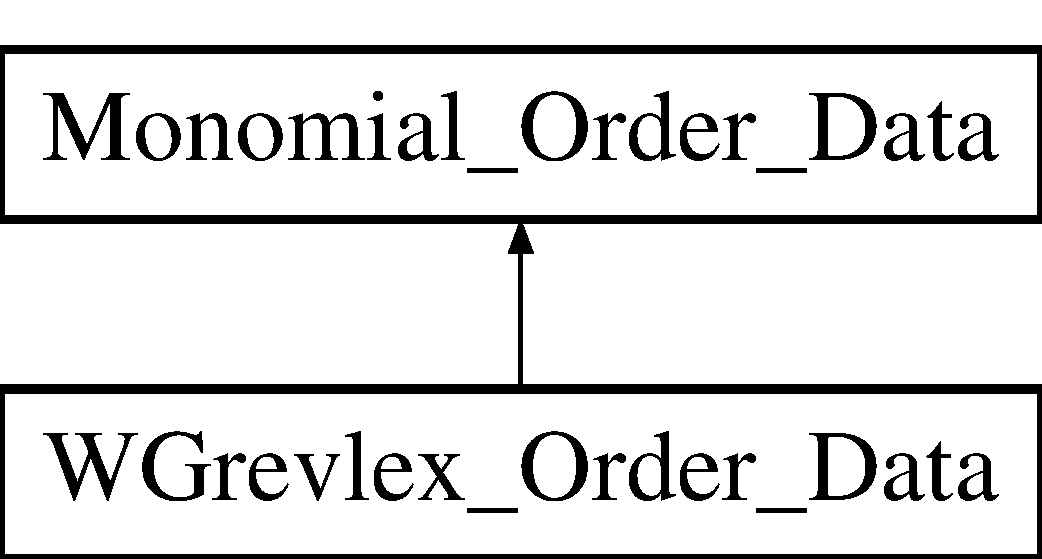
\includegraphics[height=3.000000cm]{group__orderinggroup}
\end{center}
\end{figure}
\subsubsection*{Public Member Functions}
\begin{Indent}\textbf{ Construction}\par
\begin{DoxyCompactItemize}
\item 
\hyperlink{group__orderinggroup_a107617c77aaebe5ba74973af66ab75b6}{Cached\+W\+Grevlex\+\_\+\+Ordering} (N\+V\+A\+R\+\_\+\+T\+Y\+PE number\+\_\+of\+\_\+variables, W\+T\+\_\+\+T\+Y\+PE $\ast$w, bool thorough=true)
\begin{DoxyCompactList}\small\item\em creates a weighted grevlex ordering specific to $n$ variables, using the weights specified by $w$ \end{DoxyCompactList}\end{DoxyCompactItemize}
\end{Indent}
\begin{Indent}\textbf{ Basic properties}\par
\begin{DoxyCompactItemize}
\item 
\mbox{\Hypertarget{group__orderinggroup_a4997585d5bc84222551e555eac13ebf9}\label{group__orderinggroup_a4997585d5bc84222551e555eac13ebf9}} 
virtual const W\+T\+\_\+\+T\+Y\+PE $\ast$ \hyperlink{group__orderinggroup_a4997585d5bc84222551e555eac13ebf9}{order\+\_\+weights} () const override
\begin{DoxyCompactList}\small\item\em the weights that define this ordering \end{DoxyCompactList}\item 
\mbox{\Hypertarget{group__orderinggroup_aabbf09fabf721a0f894110b0f5651730}\label{group__orderinggroup_aabbf09fabf721a0f894110b0f5651730}} 
virtual N\+V\+A\+R\+\_\+\+T\+Y\+PE \hyperlink{group__orderinggroup_aabbf09fabf721a0f894110b0f5651730}{number\+\_\+of\+\_\+weights} () const override
\begin{DoxyCompactList}\small\item\em returns the number of weights (same as number of indeterminates) \end{DoxyCompactList}\end{DoxyCompactItemize}
\end{Indent}
\begin{Indent}\textbf{ Comparison}\par
\begin{DoxyCompactItemize}
\item 
\mbox{\Hypertarget{group__orderinggroup_afcba2ade4149724f666064643e502769}\label{group__orderinggroup_afcba2ade4149724f666064643e502769}} 
virtual int \hyperlink{group__orderinggroup_afcba2ade4149724f666064643e502769}{cmp} (const \hyperlink{group__polygroup_class_monomial}{Monomial} \&, const \hyperlink{group__polygroup_class_monomial}{Monomial} \&) const override
\begin{DoxyCompactList}\small\item\em resturns 0 if they are alike; positive if first larger; negative otherwise \end{DoxyCompactList}\item 
\mbox{\Hypertarget{group__orderinggroup_a78e346a28a1dde835e487c01c7ce2b5a}\label{group__orderinggroup_a78e346a28a1dde835e487c01c7ce2b5a}} 
virtual bool \hyperlink{group__orderinggroup_a78e346a28a1dde835e487c01c7ce2b5a}{first\+\_\+larger} (const \hyperlink{group__polygroup_class_monomial}{Monomial} \&t, const \hyperlink{group__polygroup_class_monomial}{Monomial} \&u) const override
\begin{DoxyCompactList}\small\item\em returns {\ttfamily true} iff $t>u$ by sums of successively fewer exponents \end{DoxyCompactList}\item 
\mbox{\Hypertarget{group__orderinggroup_a131b09d8226c2dc5f0718f90ab8e009f}\label{group__orderinggroup_a131b09d8226c2dc5f0718f90ab8e009f}} 
virtual bool \hyperlink{group__orderinggroup_a131b09d8226c2dc5f0718f90ab8e009f}{first\+\_\+smaller} (const \hyperlink{group__polygroup_class_monomial}{Monomial} \&t, const \hyperlink{group__polygroup_class_monomial}{Monomial} \&u) const override
\begin{DoxyCompactList}\small\item\em returns {\ttfamily true} iff $t< u$ by sums of successively fewer exponents \end{DoxyCompactList}\item 
\mbox{\Hypertarget{group__orderinggroup_a7841ec558b2858c2a6eda8fd6073641e}\label{group__orderinggroup_a7841ec558b2858c2a6eda8fd6073641e}} 
virtual bool \hyperlink{group__orderinggroup_a7841ec558b2858c2a6eda8fd6073641e}{first\+\_\+larger\+\_\+than\+\_\+multiple} (const \hyperlink{group__polygroup_class_monomial}{Monomial} \&t, const \hyperlink{group__polygroup_class_monomial}{Monomial} \&u, const \hyperlink{group__polygroup_class_monomial}{Monomial} \&v) const override
\begin{DoxyCompactList}\small\item\em returns {\ttfamily true} iff $t>u$ by sums of successively fewer exponents \end{DoxyCompactList}\end{DoxyCompactItemize}
\end{Indent}
\begin{Indent}\textbf{ Utility}\par
\begin{DoxyCompactItemize}
\item 
D\+E\+G\+\_\+\+T\+Y\+PE \hyperlink{group__orderinggroup_af04f39af33cba2c1c4f985e57ea8d136}{partial\+\_\+degree} (const \hyperlink{group__polygroup_class_monomial}{Monomial} \&t, N\+V\+A\+R\+\_\+\+T\+Y\+PE i) const
\item 
D\+E\+G\+\_\+\+T\+Y\+PE \hyperlink{group__orderinggroup_a960a5b3460c4cab0dfd89bc0663c6ee0}{compute\+\_\+ith\+\_\+weight} (const \hyperlink{group__polygroup_class_monomial}{Monomial} \&t, N\+V\+A\+R\+\_\+\+T\+Y\+PE i) const
\item 
\mbox{\Hypertarget{group__orderinggroup_a65f1e27ee52413c91ffcb87632dcb27c}\label{group__orderinggroup_a65f1e27ee52413c91ffcb87632dcb27c}} 
virtual void \hyperlink{group__orderinggroup_a65f1e27ee52413c91ffcb87632dcb27c}{set\+\_\+data} (\hyperlink{group__polygroup_class_monomial}{Monomial} \&t) const override
\begin{DoxyCompactList}\small\item\em sets the \hyperlink{group__polygroup_class_monomial}{Monomial}'s {\ttfamily monomial\+\_\+ordering\+\_\+data} \end{DoxyCompactList}\end{DoxyCompactItemize}
\end{Indent}
\subsubsection*{Protected Attributes}
\begin{DoxyCompactItemize}
\item 
\mbox{\Hypertarget{group__orderinggroup_a1673ac75841fe8203941c73030621579}\label{group__orderinggroup_a1673ac75841fe8203941c73030621579}} 
const bool \hyperlink{group__orderinggroup_a1673ac75841fe8203941c73030621579}{fully\+\_\+apply}
\begin{DoxyCompactList}\small\item\em whether to apply the weights to more than the first sum \end{DoxyCompactList}\item 
\mbox{\Hypertarget{group__orderinggroup_a2857c72d3d83c1ec4dfaea5dc6fb4893}\label{group__orderinggroup_a2857c72d3d83c1ec4dfaea5dc6fb4893}} 
const N\+V\+A\+R\+\_\+\+T\+Y\+PE \hyperlink{group__orderinggroup_a2857c72d3d83c1ec4dfaea5dc6fb4893}{n}
\begin{DoxyCompactList}\small\item\em the number of variables, which should remain constant \end{DoxyCompactList}\item 
\mbox{\Hypertarget{group__orderinggroup_adb595ee1755d11ab65164222c7ec2d94}\label{group__orderinggroup_adb595ee1755d11ab65164222c7ec2d94}} 
const W\+T\+\_\+\+T\+Y\+PE $\ast$ \hyperlink{group__orderinggroup_adb595ee1755d11ab65164222c7ec2d94}{weights}
\begin{DoxyCompactList}\small\item\em the weights that define this ordering \end{DoxyCompactList}\end{DoxyCompactItemize}
\subsubsection*{Friends}
\begin{Indent}\textbf{ I/O}\par
\begin{DoxyCompactItemize}
\item 
\mbox{\Hypertarget{group__orderinggroup_a6b25de5d93b628d0cb77ec4caafca32b}\label{group__orderinggroup_a6b25de5d93b628d0cb77ec4caafca32b}} 
ostream \& {\bfseries operator$<$$<$} (ostream \&os, const \hyperlink{group__orderinggroup_class_cached_w_grevlex___ordering}{Cached\+W\+Grevlex\+\_\+\+Ordering} \&word)
\end{DoxyCompactItemize}
\end{Indent}


\paragraph{Constructor \& Destructor Documentation}
\mbox{\Hypertarget{group__orderinggroup_a107617c77aaebe5ba74973af66ab75b6}\label{group__orderinggroup_a107617c77aaebe5ba74973af66ab75b6}} 
\index{Cached\+W\+Grevlex\+\_\+\+Ordering@{Cached\+W\+Grevlex\+\_\+\+Ordering}!Cached\+W\+Grevlex\+\_\+\+Ordering@{Cached\+W\+Grevlex\+\_\+\+Ordering}}
\index{Cached\+W\+Grevlex\+\_\+\+Ordering@{Cached\+W\+Grevlex\+\_\+\+Ordering}!Cached\+W\+Grevlex\+\_\+\+Ordering@{Cached\+W\+Grevlex\+\_\+\+Ordering}}
\subparagraph{\texorpdfstring{Cached\+W\+Grevlex\+\_\+\+Ordering()}{CachedWGrevlex\_Ordering()}}
{\footnotesize\ttfamily Cached\+W\+Grevlex\+\_\+\+Ordering\+::\+Cached\+W\+Grevlex\+\_\+\+Ordering (\begin{DoxyParamCaption}\item[{N\+V\+A\+R\+\_\+\+T\+Y\+PE}]{number\+\_\+of\+\_\+variables,  }\item[{W\+T\+\_\+\+T\+Y\+PE $\ast$}]{w,  }\item[{bool}]{thorough = {\ttfamily true} }\end{DoxyParamCaption})}



creates a weighted grevlex ordering specific to $n$ variables, using the weights specified by $w$ 


\begin{DoxyParams}{Parameters}
{\em thorough} & determines whether the weights are applied to subsequent orderings; if {\ttfamily false}, the second, third, etc. sums are ordinary sums of the exponents, rather than weighted sums \\
\hline
{\em number\+\_\+of\+\_\+variables} & the number of variables this will compare; {\ttfamily weights} should have this length! \\
\hline
{\em w} & the weights to multiply to each exponent \\
\hline
\end{DoxyParams}


Definition at line 431 of file particular\+\_\+orderings.\+cpp.



\paragraph{Member Function Documentation}
\mbox{\Hypertarget{group__orderinggroup_a960a5b3460c4cab0dfd89bc0663c6ee0}\label{group__orderinggroup_a960a5b3460c4cab0dfd89bc0663c6ee0}} 
\index{Cached\+W\+Grevlex\+\_\+\+Ordering@{Cached\+W\+Grevlex\+\_\+\+Ordering}!compute\+\_\+ith\+\_\+weight@{compute\+\_\+ith\+\_\+weight}}
\index{compute\+\_\+ith\+\_\+weight@{compute\+\_\+ith\+\_\+weight}!Cached\+W\+Grevlex\+\_\+\+Ordering@{Cached\+W\+Grevlex\+\_\+\+Ordering}}
\subparagraph{\texorpdfstring{compute\+\_\+ith\+\_\+weight()}{compute\_ith\_weight()}}
{\footnotesize\ttfamily D\+E\+G\+\_\+\+T\+Y\+PE Cached\+W\+Grevlex\+\_\+\+Ordering\+::compute\+\_\+ith\+\_\+weight (\begin{DoxyParamCaption}\item[{const \hyperlink{group__polygroup_class_monomial}{Monomial} \&}]{t,  }\item[{N\+V\+A\+R\+\_\+\+T\+Y\+PE}]{i }\end{DoxyParamCaption}) const}

\begin{DoxyReturn}{Returns}
the sum of the first i exponents 
\end{DoxyReturn}

\begin{DoxyParams}{Parameters}
{\em t} & a \hyperlink{group__polygroup_class_monomial}{Monomial} whose degree we want \\
\hline
{\em i} & index to an exponent \\
\hline
\end{DoxyParams}


Definition at line 527 of file particular\+\_\+orderings.\+cpp.

\mbox{\Hypertarget{group__orderinggroup_af04f39af33cba2c1c4f985e57ea8d136}\label{group__orderinggroup_af04f39af33cba2c1c4f985e57ea8d136}} 
\index{Cached\+W\+Grevlex\+\_\+\+Ordering@{Cached\+W\+Grevlex\+\_\+\+Ordering}!partial\+\_\+degree@{partial\+\_\+degree}}
\index{partial\+\_\+degree@{partial\+\_\+degree}!Cached\+W\+Grevlex\+\_\+\+Ordering@{Cached\+W\+Grevlex\+\_\+\+Ordering}}
\subparagraph{\texorpdfstring{partial\+\_\+degree()}{partial\_degree()}}
{\footnotesize\ttfamily D\+E\+G\+\_\+\+T\+Y\+PE Cached\+W\+Grevlex\+\_\+\+Ordering\+::partial\+\_\+degree (\begin{DoxyParamCaption}\item[{const \hyperlink{group__polygroup_class_monomial}{Monomial} \&}]{t,  }\item[{N\+V\+A\+R\+\_\+\+T\+Y\+PE}]{i }\end{DoxyParamCaption}) const\hspace{0.3cm}{\ttfamily [inline]}}

\begin{DoxyReturn}{Returns}
the weighted sum of the first i exponents 
\end{DoxyReturn}

\begin{DoxyParams}{Parameters}
{\em t} & a \hyperlink{group__polygroup_class_monomial}{Monomial} whose degree we want \\
\hline
{\em i} & index to an exponent \\
\hline
\end{DoxyParams}
\begin{DoxyWarning}{Warning}
Be sure that {\ttfamily t} has the correct ordering! 
\end{DoxyWarning}


Definition at line 517 of file particular\+\_\+orderings.\+hpp.

\index{Generic\+\_\+\+Grevlex@{Generic\+\_\+\+Grevlex}}\label{class_generic___grevlex}
\Hypertarget{group__orderinggroup_class_generic___grevlex}
\subsubsection{class Generic\+\_\+\+Grevlex}
generic grevlex ordering, works with any number of variables 

\begin{DoxyAuthor}{Author}
John Perry 
\end{DoxyAuthor}
\begin{DoxyDate}{Date}
2015
\end{DoxyDate}
The difference between \hyperlink{group__orderinggroup_class_generic___grevlex}{Generic\+\_\+\+Grevlex} and \hyperlink{group__orderinggroup_class_grevlex___ordering}{Grevlex\+\_\+\+Ordering} is that the former doesn't track any \hyperlink{group__orderinggroup_class_monomial___order___data}{Monomial\+\_\+\+Order\+\_\+\+Data}, while the latter relies on it. The latter should, as a result, be more time efficient, while the former is more space efficient. \hyperlink{group__orderinggroup_class_generic___grevlex}{Generic\+\_\+\+Grevlex} will also order monomials which by design have a different number of variables, though that should not in general be something one encounters, and it's rather dangerous with \hyperlink{group__orderinggroup_a1696724ba30a8565b759bb2c8aeefde4}{first\+\_\+larger\+\_\+than\+\_\+multiple()}. 

Definition at line 46 of file particular\+\_\+orderings.\+hpp.

Inheritance diagram for Generic\+\_\+\+Grevlex\+:\begin{figure}[H]
\begin{center}
\leavevmode
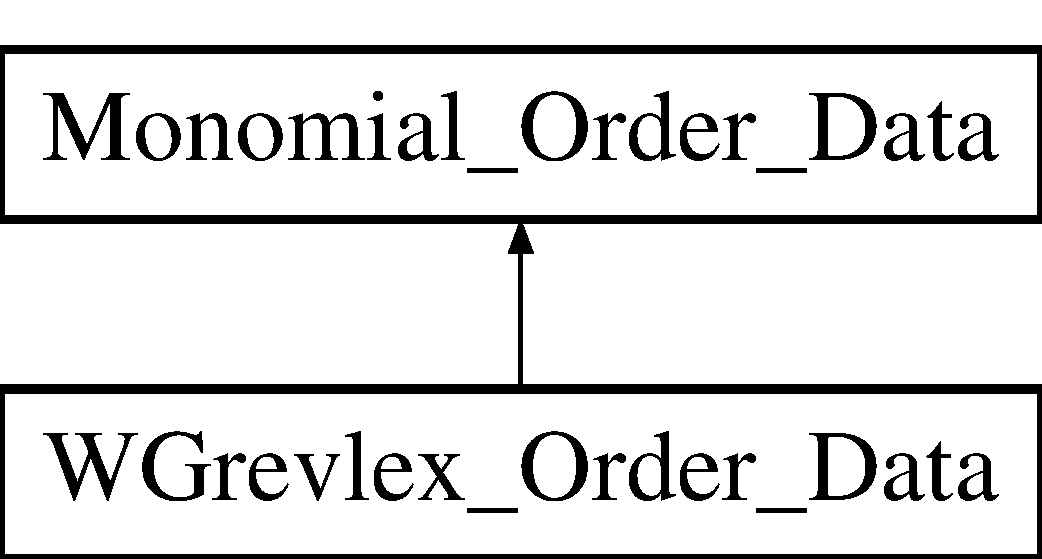
\includegraphics[height=2.000000cm]{group__orderinggroup}
\end{center}
\end{figure}
\subsubsection*{Public Member Functions}
\begin{Indent}\textbf{ Comparison}\par
\begin{DoxyCompactItemize}
\item 
\mbox{\Hypertarget{group__orderinggroup_ac412c73e940b4aabe1e350d6c98a99f5}\label{group__orderinggroup_ac412c73e940b4aabe1e350d6c98a99f5}} 
virtual bool \hyperlink{group__orderinggroup_ac412c73e940b4aabe1e350d6c98a99f5}{first\+\_\+larger} (const \hyperlink{group__polygroup_class_monomial}{Monomial} \&, const \hyperlink{group__polygroup_class_monomial}{Monomial} \&) const override
\begin{DoxyCompactList}\small\item\em returns {\ttfamily true} iff the first \hyperlink{group__polygroup_class_monomial}{Monomial} is larger than the second \end{DoxyCompactList}\item 
\mbox{\Hypertarget{group__orderinggroup_a48ba39468e17d826988b28f5d871d868}\label{group__orderinggroup_a48ba39468e17d826988b28f5d871d868}} 
virtual bool \hyperlink{group__orderinggroup_a48ba39468e17d826988b28f5d871d868}{first\+\_\+smaller} (const \hyperlink{group__polygroup_class_monomial}{Monomial} \&, const \hyperlink{group__polygroup_class_monomial}{Monomial} \&) const override
\begin{DoxyCompactList}\small\item\em returns {\ttfamily true} iff the first \hyperlink{group__polygroup_class_monomial}{Monomial} is smaller than the second \end{DoxyCompactList}\item 
\mbox{\Hypertarget{group__orderinggroup_a1696724ba30a8565b759bb2c8aeefde4}\label{group__orderinggroup_a1696724ba30a8565b759bb2c8aeefde4}} 
virtual bool \hyperlink{group__orderinggroup_a1696724ba30a8565b759bb2c8aeefde4}{first\+\_\+larger\+\_\+than\+\_\+multiple} (const \hyperlink{group__polygroup_class_monomial}{Monomial} \&, const \hyperlink{group__polygroup_class_monomial}{Monomial} \&, const \hyperlink{group__polygroup_class_monomial}{Monomial} \&) const override
\begin{DoxyCompactList}\small\item\em returns {\ttfamily true} iff the first \hyperlink{group__polygroup_class_monomial}{Monomial} is larger than the product of the second and the third \end{DoxyCompactList}\item 
virtual int \hyperlink{group__orderinggroup_ae7103c92d45f749eaf3c5403b17a2828}{cmp} (const \hyperlink{group__polygroup_class_monomial}{Monomial} \&t, const \hyperlink{group__polygroup_class_monomial}{Monomial} \&u) const override
\end{DoxyCompactItemize}
\end{Indent}
\begin{Indent}\textbf{ Utility}\par
{\em sets the \hyperlink{group__polygroup_class_monomial}{Monomial}'s {\ttfamily monomial\+\_\+ordering\+\_\+data} }\begin{DoxyCompactItemize}
\item 
virtual void \hyperlink{group__orderinggroup_a14c344858da03d16c8019afdae3da5dc}{set\+\_\+data} (\hyperlink{group__polygroup_class_monomial}{Monomial} \&t) const override
\begin{DoxyCompactList}\small\item\em sets monomial ordering's data; default is to do nothing \end{DoxyCompactList}\end{DoxyCompactItemize}
\end{Indent}


\paragraph{Member Function Documentation}
\mbox{\Hypertarget{group__orderinggroup_ae7103c92d45f749eaf3c5403b17a2828}\label{group__orderinggroup_ae7103c92d45f749eaf3c5403b17a2828}} 
\index{Generic\+\_\+\+Grevlex@{Generic\+\_\+\+Grevlex}!cmp@{cmp}}
\index{cmp@{cmp}!Generic\+\_\+\+Grevlex@{Generic\+\_\+\+Grevlex}}
\subparagraph{\texorpdfstring{cmp()}{cmp()}}
{\footnotesize\ttfamily virtual int Generic\+\_\+\+Grevlex\+::cmp (\begin{DoxyParamCaption}\item[{const \hyperlink{group__polygroup_class_monomial}{Monomial} \&}]{t,  }\item[{const \hyperlink{group__polygroup_class_monomial}{Monomial} \&}]{u }\end{DoxyParamCaption}) const\hspace{0.3cm}{\ttfamily [inline]}, {\ttfamily [override]}, {\ttfamily [virtual]}}


\begin{DoxyParams}{Parameters}
{\em t} & a \hyperlink{group__polygroup_class_monomial}{Monomial}, to compare to $ u $ \\
\hline
{\em u} & a \hyperlink{group__polygroup_class_monomial}{Monomial}, to compare to $ t $ \\
\hline
\end{DoxyParams}
\begin{DoxyReturn}{Returns}
1 if $ t > u $ , -\/1 if $ t < u $ , and 0 otherwise 
\end{DoxyReturn}


Implements \hyperlink{group__orderinggroup_a9bc3155fc98b4d40c26118fa2114b827}{Monomial\+\_\+\+Ordering}.



Definition at line 66 of file particular\+\_\+orderings.\+hpp.

\mbox{\Hypertarget{group__orderinggroup_a14c344858da03d16c8019afdae3da5dc}\label{group__orderinggroup_a14c344858da03d16c8019afdae3da5dc}} 
\index{Generic\+\_\+\+Grevlex@{Generic\+\_\+\+Grevlex}!set\+\_\+data@{set\+\_\+data}}
\index{set\+\_\+data@{set\+\_\+data}!Generic\+\_\+\+Grevlex@{Generic\+\_\+\+Grevlex}}
\subparagraph{\texorpdfstring{set\+\_\+data()}{set\_data()}}
{\footnotesize\ttfamily void Generic\+\_\+\+Grevlex\+::set\+\_\+data (\begin{DoxyParamCaption}\item[{\hyperlink{group__polygroup_class_monomial}{Monomial} \&}]{t }\end{DoxyParamCaption}) const\hspace{0.3cm}{\ttfamily [override]}, {\ttfamily [virtual]}}



sets monomial ordering's data; default is to do nothing 

Child classes that override this function are strongly recommended to use set\+\_\+ordering\+\_\+degree() of the \hyperlink{group__polygroup_class_monomial}{Monomial} class to set a primary degree. For weighted/graded degree orderings, this typically improves performance nontrivially. 

Reimplemented from \hyperlink{group__orderinggroup_a22b08dffd1cdf3a655ca18d604cfcee1}{Monomial\+\_\+\+Ordering}.



Definition at line 54 of file particular\+\_\+orderings.\+cpp.

\index{Grevlex\+\_\+\+Order\+\_\+\+Data@{Grevlex\+\_\+\+Order\+\_\+\+Data}}\label{class_grevlex___order___data}
\Hypertarget{group__orderinggroup_class_grevlex___order___data}
\subsubsection{class Grevlex\+\_\+\+Order\+\_\+\+Data}
data for the grevlex monomial ordering 

\begin{DoxyAuthor}{Author}
John Perry 
\end{DoxyAuthor}
\begin{DoxyDate}{Date}
2015
\end{DoxyDate}
The data involves an array of $n$ {\ttfamily D\+E\+G\+\_\+\+T\+Y\+PE}, where the first entry is the sum of the first $n$ variables, the second entry is the sum of all but the last variable, etc. 

Definition at line 100 of file particular\+\_\+orderings.\+hpp.

Inheritance diagram for Grevlex\+\_\+\+Order\+\_\+\+Data\+:\begin{figure}[H]
\begin{center}
\leavevmode
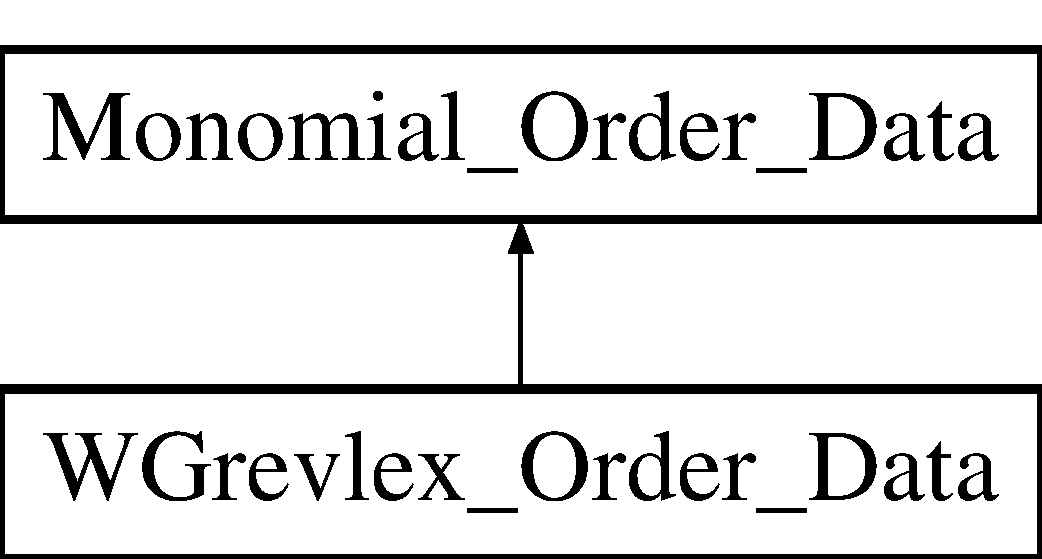
\includegraphics[height=2.000000cm]{group__orderinggroup}
\end{center}
\end{figure}
\subsubsection*{Public Member Functions}
\begin{Indent}\textbf{ Construction}\par
\begin{DoxyCompactItemize}
\item 
\hyperlink{group__orderinggroup_a61000659db1597c1fb7f149deb0d952c}{Grevlex\+\_\+\+Order\+\_\+\+Data} (const \hyperlink{group__polygroup_class_monomial}{Monomial} \&t)
\begin{DoxyCompactList}\small\item\em creates an array of partial weights of {\ttfamily t} \end{DoxyCompactList}\item 
\mbox{\Hypertarget{group__orderinggroup_a53b3cafb2c36cea8c58aba05eeb422ea}\label{group__orderinggroup_a53b3cafb2c36cea8c58aba05eeb422ea}} 
\hyperlink{group__orderinggroup_a53b3cafb2c36cea8c58aba05eeb422ea}{Grevlex\+\_\+\+Order\+\_\+\+Data} (const \hyperlink{group__orderinggroup_class_grevlex___order___data}{Grevlex\+\_\+\+Order\+\_\+\+Data} \&)
\begin{DoxyCompactList}\small\item\em copy constructor \end{DoxyCompactList}\item 
\mbox{\Hypertarget{group__orderinggroup_a001fd11460120bb1df89f4960ec9d800}\label{group__orderinggroup_a001fd11460120bb1df89f4960ec9d800}} 
virtual \hyperlink{group__orderinggroup_class_grevlex___order___data}{Grevlex\+\_\+\+Order\+\_\+\+Data} $\ast$ \hyperlink{group__orderinggroup_a001fd11460120bb1df89f4960ec9d800}{clone} () override
\begin{DoxyCompactList}\small\item\em clone ``constructor'' \end{DoxyCompactList}\end{DoxyCompactItemize}
\end{Indent}
\begin{Indent}\textbf{ Destruction}\par
\begin{DoxyCompactItemize}
\item 
\mbox{\Hypertarget{group__orderinggroup_a275afe22c3514d5602eda962402821c3}\label{group__orderinggroup_a275afe22c3514d5602eda962402821c3}} 
\hyperlink{group__orderinggroup_a275afe22c3514d5602eda962402821c3}{$\sim$\+Grevlex\+\_\+\+Order\+\_\+\+Data} ()
\begin{DoxyCompactList}\small\item\em deletes the array creates by the constructor \end{DoxyCompactList}\end{DoxyCompactItemize}
\end{Indent}
\begin{Indent}\textbf{ Basic properties}\par
\begin{DoxyCompactItemize}
\item 
\mbox{\Hypertarget{group__orderinggroup_aa493ca0ff50ec991894bb95de918e12b}\label{group__orderinggroup_aa493ca0ff50ec991894bb95de918e12b}} 
D\+E\+G\+\_\+\+T\+Y\+PE \hyperlink{group__orderinggroup_aa493ca0ff50ec991894bb95de918e12b}{operator\mbox{[}$\,$\mbox{]}} (N\+V\+A\+R\+\_\+\+T\+Y\+PE i) const
\begin{DoxyCompactList}\small\item\em returns the sum of the first $i$ variables' exponents \end{DoxyCompactList}\item 
\mbox{\Hypertarget{group__orderinggroup_a93ade17bec5b9628d3ed02a776835ee0}\label{group__orderinggroup_a93ade17bec5b9628d3ed02a776835ee0}} 
virtual D\+E\+G\+\_\+\+T\+Y\+PE \hyperlink{group__orderinggroup_a93ade17bec5b9628d3ed02a776835ee0}{grading} (N\+V\+A\+R\+\_\+\+T\+Y\+PE i) const override
\begin{DoxyCompactList}\small\item\em default value is useless; orderings that supply gradings should redefine \end{DoxyCompactList}\end{DoxyCompactItemize}
\end{Indent}
\begin{Indent}\textbf{ Computation}\par
\begin{DoxyCompactItemize}
\item 
void \hyperlink{group__orderinggroup_aeaf81375ec0b27a6e9c047b1d63c6d55}{assign\+\_\+gradings} (const \hyperlink{group__polygroup_class_monomial}{Monomial} \&)
\begin{DoxyCompactList}\small\item\em assigns gradings to a pre-\/allocated array \end{DoxyCompactList}\end{DoxyCompactItemize}
\end{Indent}
\subsubsection*{Protected Attributes}
\begin{DoxyCompactItemize}
\item 
\mbox{\Hypertarget{group__orderinggroup_a0a4ccd9abf8d598bdb64b015f127bf4e}\label{group__orderinggroup_a0a4ccd9abf8d598bdb64b015f127bf4e}} 
D\+E\+G\+\_\+\+T\+Y\+PE $\ast$ \hyperlink{group__orderinggroup_a0a4ccd9abf8d598bdb64b015f127bf4e}{gradings}
\begin{DoxyCompactList}\small\item\em list of partial sums of exponents \end{DoxyCompactList}\item 
\mbox{\Hypertarget{group__orderinggroup_afaddc36a549cd365d5f10bd817ddbef5}\label{group__orderinggroup_afaddc36a549cd365d5f10bd817ddbef5}} 
const N\+V\+A\+R\+\_\+\+T\+Y\+PE \hyperlink{group__orderinggroup_afaddc36a549cd365d5f10bd817ddbef5}{number\+\_\+of\+\_\+gradings}
\begin{DoxyCompactList}\small\item\em length of {\ttfamily gradings} \end{DoxyCompactList}\end{DoxyCompactItemize}


\paragraph{Constructor \& Destructor Documentation}
\mbox{\Hypertarget{group__orderinggroup_a61000659db1597c1fb7f149deb0d952c}\label{group__orderinggroup_a61000659db1597c1fb7f149deb0d952c}} 
\index{Grevlex\+\_\+\+Order\+\_\+\+Data@{Grevlex\+\_\+\+Order\+\_\+\+Data}!Grevlex\+\_\+\+Order\+\_\+\+Data@{Grevlex\+\_\+\+Order\+\_\+\+Data}}
\index{Grevlex\+\_\+\+Order\+\_\+\+Data@{Grevlex\+\_\+\+Order\+\_\+\+Data}!Grevlex\+\_\+\+Order\+\_\+\+Data@{Grevlex\+\_\+\+Order\+\_\+\+Data}}
\subparagraph{\texorpdfstring{Grevlex\+\_\+\+Order\+\_\+\+Data()}{Grevlex\_Order\_Data()}}
{\footnotesize\ttfamily Grevlex\+\_\+\+Order\+\_\+\+Data\+::\+Grevlex\+\_\+\+Order\+\_\+\+Data (\begin{DoxyParamCaption}\item[{const \hyperlink{group__polygroup_class_monomial}{Monomial} \&}]{t }\end{DoxyParamCaption})}



creates an array of partial weights of {\ttfamily t} 


\begin{DoxyParams}{Parameters}
{\em t} & a \hyperlink{group__polygroup_class_monomial}{Monomial} whose parial weights {\ttfamily this} caches \\
\hline
\end{DoxyParams}


Definition at line 231 of file particular\+\_\+orderings.\+cpp.



\paragraph{Member Function Documentation}
\mbox{\Hypertarget{group__orderinggroup_aeaf81375ec0b27a6e9c047b1d63c6d55}\label{group__orderinggroup_aeaf81375ec0b27a6e9c047b1d63c6d55}} 
\index{Grevlex\+\_\+\+Order\+\_\+\+Data@{Grevlex\+\_\+\+Order\+\_\+\+Data}!assign\+\_\+gradings@{assign\+\_\+gradings}}
\index{assign\+\_\+gradings@{assign\+\_\+gradings}!Grevlex\+\_\+\+Order\+\_\+\+Data@{Grevlex\+\_\+\+Order\+\_\+\+Data}}
\subparagraph{\texorpdfstring{assign\+\_\+gradings()}{assign\_gradings()}}
{\footnotesize\ttfamily void Grevlex\+\_\+\+Order\+\_\+\+Data\+::assign\+\_\+gradings (\begin{DoxyParamCaption}\item[{const \hyperlink{group__polygroup_class_monomial}{Monomial} \&}]{t }\end{DoxyParamCaption})}



assigns gradings to a pre-\/allocated array 

\begin{DoxyWarning}{Warning}
This does not create the array if it does not exist already! 
\end{DoxyWarning}


Definition at line 223 of file particular\+\_\+orderings.\+cpp.

\index{Grevlex\+\_\+\+Ordering@{Grevlex\+\_\+\+Ordering}}\label{class_grevlex___ordering}
\Hypertarget{group__orderinggroup_class_grevlex___ordering}
\subsubsection{class Grevlex\+\_\+\+Ordering}
the grevlex ordering for a specified number of variables 

\begin{DoxyAuthor}{Author}
John Perry 
\end{DoxyAuthor}
\begin{DoxyDate}{Date}
2015
\end{DoxyDate}
The grevlex ordering first compares the sums of the exponents, then the sums of all but the last exponent, then the sums of all but the last two exponents, and so forth, until either the sums differ or it runs out of variables. \begin{Desc}
\item[Examples\+: ]\par
\hyperlink{test_cyclicn_8cpp-example}{test\+\_\+cyclicn.\+cpp}.\end{Desc}


Definition at line 153 of file particular\+\_\+orderings.\+hpp.

Inheritance diagram for Grevlex\+\_\+\+Ordering\+:\begin{figure}[H]
\begin{center}
\leavevmode
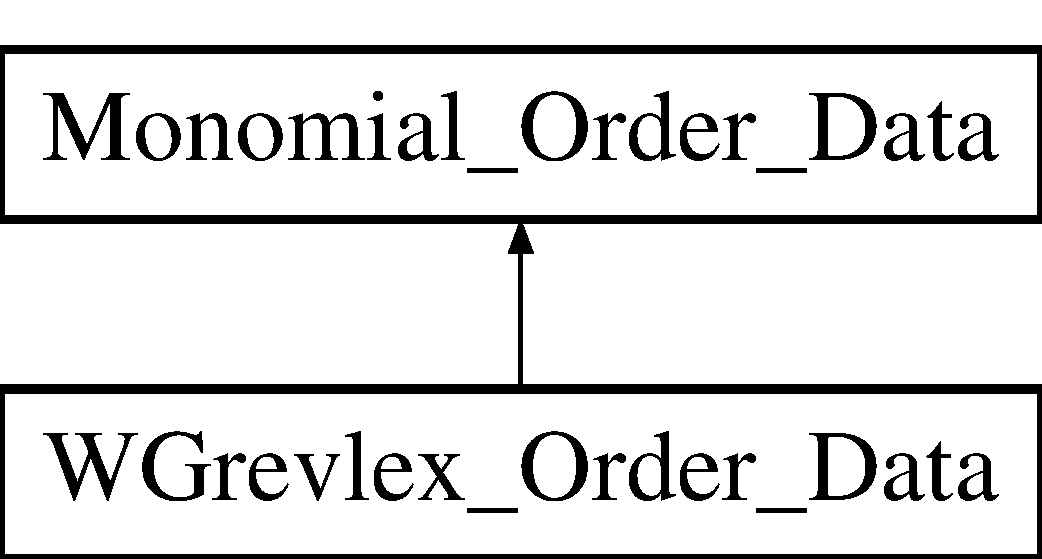
\includegraphics[height=2.000000cm]{group__orderinggroup}
\end{center}
\end{figure}
\subsubsection*{Public Member Functions}
\begin{Indent}\textbf{ Construction}\par
\begin{DoxyCompactItemize}
\item 
\mbox{\Hypertarget{group__orderinggroup_a73efa1ac5de7104f4de26d6b2c1246ba}\label{group__orderinggroup_a73efa1ac5de7104f4de26d6b2c1246ba}} 
\hyperlink{group__orderinggroup_a73efa1ac5de7104f4de26d6b2c1246ba}{Grevlex\+\_\+\+Ordering} (N\+V\+A\+R\+\_\+\+T\+Y\+PE number\+\_\+of\+\_\+variables)
\begin{DoxyCompactList}\small\item\em creates a grevlex ordering specific to the specified number of variables \end{DoxyCompactList}\end{DoxyCompactItemize}
\end{Indent}
\begin{Indent}\textbf{ Comparison}\par
\begin{DoxyCompactItemize}
\item 
\mbox{\Hypertarget{group__orderinggroup_a7ed2a24b293d63e26c0cdbe4270682a8}\label{group__orderinggroup_a7ed2a24b293d63e26c0cdbe4270682a8}} 
virtual bool \hyperlink{group__orderinggroup_a7ed2a24b293d63e26c0cdbe4270682a8}{first\+\_\+larger} (const \hyperlink{group__polygroup_class_monomial}{Monomial} \&t, const \hyperlink{group__polygroup_class_monomial}{Monomial} \&u) const override
\begin{DoxyCompactList}\small\item\em returns {\ttfamily true} iff $t>u$ by sums of successively fewer exponents \end{DoxyCompactList}\item 
\mbox{\Hypertarget{group__orderinggroup_abb1afdfa6ace5b90e425d0645e278c67}\label{group__orderinggroup_abb1afdfa6ace5b90e425d0645e278c67}} 
virtual bool \hyperlink{group__orderinggroup_abb1afdfa6ace5b90e425d0645e278c67}{first\+\_\+smaller} (const \hyperlink{group__polygroup_class_monomial}{Monomial} \&t, const \hyperlink{group__polygroup_class_monomial}{Monomial} \&u) const override
\begin{DoxyCompactList}\small\item\em returns {\ttfamily true} iff $t< u$ by sums of successively fewer exponents \end{DoxyCompactList}\item 
virtual bool \hyperlink{group__orderinggroup_a4f8a9207711dabeb940fba0e32f4ab1f}{first\+\_\+larger\+\_\+than\+\_\+multiple} (const \hyperlink{group__polygroup_class_monomial}{Monomial} \&t, const \hyperlink{group__polygroup_class_monomial}{Monomial} \&u, const \hyperlink{group__polygroup_class_monomial}{Monomial} \&v) const override
\item 
D\+E\+G\+\_\+\+T\+Y\+PE \hyperlink{group__orderinggroup_a24d2e7bf28ecab1d8a6c703147f48341}{partial\+\_\+degree} (const \hyperlink{group__polygroup_class_monomial}{Monomial} \&t, N\+V\+A\+R\+\_\+\+T\+Y\+PE i) const
\item 
virtual int \hyperlink{group__orderinggroup_a1b668700d9ccc218ebae6049bb76fb07}{cmp} (const \hyperlink{group__polygroup_class_monomial}{Monomial} \&t, const \hyperlink{group__polygroup_class_monomial}{Monomial} \&u) const override
\end{DoxyCompactItemize}
\end{Indent}
\begin{Indent}\textbf{ Utility}\par
\begin{DoxyCompactItemize}
\item 
\mbox{\Hypertarget{group__orderinggroup_a8c65377ef8f3015a6c03ef933b37550a}\label{group__orderinggroup_a8c65377ef8f3015a6c03ef933b37550a}} 
D\+E\+G\+\_\+\+T\+Y\+PE \hyperlink{group__orderinggroup_a8c65377ef8f3015a6c03ef933b37550a}{compute\+\_\+ith\+\_\+weight} (const \hyperlink{group__polygroup_class_monomial}{Monomial} \&t, N\+V\+A\+R\+\_\+\+T\+Y\+PE i) const
\begin{DoxyCompactList}\small\item\em computes the sum of the first i exponents \end{DoxyCompactList}\item 
\mbox{\Hypertarget{group__orderinggroup_a83abd3e7505fe2096b01b8146bfdd83f}\label{group__orderinggroup_a83abd3e7505fe2096b01b8146bfdd83f}} 
virtual void \hyperlink{group__orderinggroup_a83abd3e7505fe2096b01b8146bfdd83f}{set\+\_\+data} (\hyperlink{group__polygroup_class_monomial}{Monomial} \&t) const override
\begin{DoxyCompactList}\small\item\em sets the \hyperlink{group__polygroup_class_monomial}{Monomial}'s {\ttfamily monomial\+\_\+ordering\+\_\+data} \end{DoxyCompactList}\end{DoxyCompactItemize}
\end{Indent}
\subsubsection*{Protected Attributes}
\begin{DoxyCompactItemize}
\item 
\mbox{\Hypertarget{group__orderinggroup_a3fa495befedef829c12097e239fea97f}\label{group__orderinggroup_a3fa495befedef829c12097e239fea97f}} 
const N\+V\+A\+R\+\_\+\+T\+Y\+PE \hyperlink{group__orderinggroup_a3fa495befedef829c12097e239fea97f}{n}
\begin{DoxyCompactList}\small\item\em the number of variables, which should remain constant \end{DoxyCompactList}\end{DoxyCompactItemize}


\paragraph{Member Function Documentation}
\mbox{\Hypertarget{group__orderinggroup_a1b668700d9ccc218ebae6049bb76fb07}\label{group__orderinggroup_a1b668700d9ccc218ebae6049bb76fb07}} 
\index{Grevlex\+\_\+\+Ordering@{Grevlex\+\_\+\+Ordering}!cmp@{cmp}}
\index{cmp@{cmp}!Grevlex\+\_\+\+Ordering@{Grevlex\+\_\+\+Ordering}}
\subparagraph{\texorpdfstring{cmp()}{cmp()}}
{\footnotesize\ttfamily virtual int Grevlex\+\_\+\+Ordering\+::cmp (\begin{DoxyParamCaption}\item[{const \hyperlink{group__polygroup_class_monomial}{Monomial} \&}]{t,  }\item[{const \hyperlink{group__polygroup_class_monomial}{Monomial} \&}]{u }\end{DoxyParamCaption}) const\hspace{0.3cm}{\ttfamily [inline]}, {\ttfamily [override]}, {\ttfamily [virtual]}}


\begin{DoxyParams}{Parameters}
{\em t} & a \hyperlink{group__polygroup_class_monomial}{Monomial}, to compare to $ u $ \\
\hline
{\em u} & a \hyperlink{group__polygroup_class_monomial}{Monomial}, to compare to $ t $ \\
\hline
\end{DoxyParams}
\begin{DoxyReturn}{Returns}
1 if $ t > u $ , -\/1 if $ t < u $ , and 0 otherwise 
\end{DoxyReturn}


Implements \hyperlink{group__orderinggroup_a9bc3155fc98b4d40c26118fa2114b827}{Monomial\+\_\+\+Ordering}.



Definition at line 193 of file particular\+\_\+orderings.\+hpp.

\mbox{\Hypertarget{group__orderinggroup_a4f8a9207711dabeb940fba0e32f4ab1f}\label{group__orderinggroup_a4f8a9207711dabeb940fba0e32f4ab1f}} 
\index{Grevlex\+\_\+\+Ordering@{Grevlex\+\_\+\+Ordering}!first\+\_\+larger\+\_\+than\+\_\+multiple@{first\+\_\+larger\+\_\+than\+\_\+multiple}}
\index{first\+\_\+larger\+\_\+than\+\_\+multiple@{first\+\_\+larger\+\_\+than\+\_\+multiple}!Grevlex\+\_\+\+Ordering@{Grevlex\+\_\+\+Ordering}}
\subparagraph{\texorpdfstring{first\+\_\+larger\+\_\+than\+\_\+multiple()}{first\_larger\_than\_multiple()}}
{\footnotesize\ttfamily bool Grevlex\+\_\+\+Ordering\+::first\+\_\+larger\+\_\+than\+\_\+multiple (\begin{DoxyParamCaption}\item[{const \hyperlink{group__polygroup_class_monomial}{Monomial} \&}]{t,  }\item[{const \hyperlink{group__polygroup_class_monomial}{Monomial} \&}]{u,  }\item[{const \hyperlink{group__polygroup_class_monomial}{Monomial} \&}]{v }\end{DoxyParamCaption}) const\hspace{0.3cm}{\ttfamily [override]}, {\ttfamily [virtual]}}


\begin{DoxyParams}{Parameters}
{\em t} & a \hyperlink{group__polygroup_class_monomial}{Monomial}, to compare to $ uv $ \\
\hline
{\em u} & a \hyperlink{group__polygroup_class_monomial}{Monomial}, to multiply to $ v $ \\
\hline
{\em v} & a \hyperlink{group__polygroup_class_monomial}{Monomial}, to multiply to $ u $ \\
\hline
\end{DoxyParams}
\begin{DoxyReturn}{Returns}
{\ttfamily true} iff $t>uv$ 
\end{DoxyReturn}


Implements \hyperlink{group__orderinggroup_aacb0439b908d45cc5f2635567c6633fd}{Monomial\+\_\+\+Ordering}.



Definition at line 295 of file particular\+\_\+orderings.\+cpp.

\mbox{\Hypertarget{group__orderinggroup_a24d2e7bf28ecab1d8a6c703147f48341}\label{group__orderinggroup_a24d2e7bf28ecab1d8a6c703147f48341}} 
\index{Grevlex\+\_\+\+Ordering@{Grevlex\+\_\+\+Ordering}!partial\+\_\+degree@{partial\+\_\+degree}}
\index{partial\+\_\+degree@{partial\+\_\+degree}!Grevlex\+\_\+\+Ordering@{Grevlex\+\_\+\+Ordering}}
\subparagraph{\texorpdfstring{partial\+\_\+degree()}{partial\_degree()}}
{\footnotesize\ttfamily D\+E\+G\+\_\+\+T\+Y\+PE Grevlex\+\_\+\+Ordering\+::partial\+\_\+degree (\begin{DoxyParamCaption}\item[{const \hyperlink{group__polygroup_class_monomial}{Monomial} \&}]{t,  }\item[{N\+V\+A\+R\+\_\+\+T\+Y\+PE}]{i }\end{DoxyParamCaption}) const}

\begin{DoxyReturn}{Returns}
the weighted sum of the first i exponents 
\end{DoxyReturn}
\begin{DoxyWarning}{Warning}
Be sure that {\ttfamily t} has the correct ordering! 
\end{DoxyWarning}

\begin{DoxyParams}{Parameters}
{\em t} & a \hyperlink{group__polygroup_class_monomial}{Monomial} whose partial degree we want \\
\hline
{\em i} & index of the indeterminate to which we compute the degree \\
\hline
\end{DoxyParams}


Definition at line 314 of file particular\+\_\+orderings.\+cpp.

\index{Lex\+\_\+\+Ordering@{Lex\+\_\+\+Ordering}}\label{class_lex___ordering}
\Hypertarget{group__orderinggroup_class_lex___ordering}
\subsubsection{class Lex\+\_\+\+Ordering}
the lex ordering for a specified number of variables 

\begin{DoxyAuthor}{Author}
John Perry 
\end{DoxyAuthor}
\begin{DoxyDate}{Date}
2015
\end{DoxyDate}
The lex ordering is a dictionary ordering. The first variable is considered largest, and monomials with a larger degree in the first variable will be considered larger than monomials with a smaller degree in the first variable, regardless of the overall degree in all variables. \begin{Desc}
\item[Examples\+: ]\par
\hyperlink{test_cyclicn_8cpp-example}{test\+\_\+cyclicn.\+cpp}.\end{Desc}


Definition at line 339 of file particular\+\_\+orderings.\+hpp.

Inheritance diagram for Lex\+\_\+\+Ordering\+:\begin{figure}[H]
\begin{center}
\leavevmode
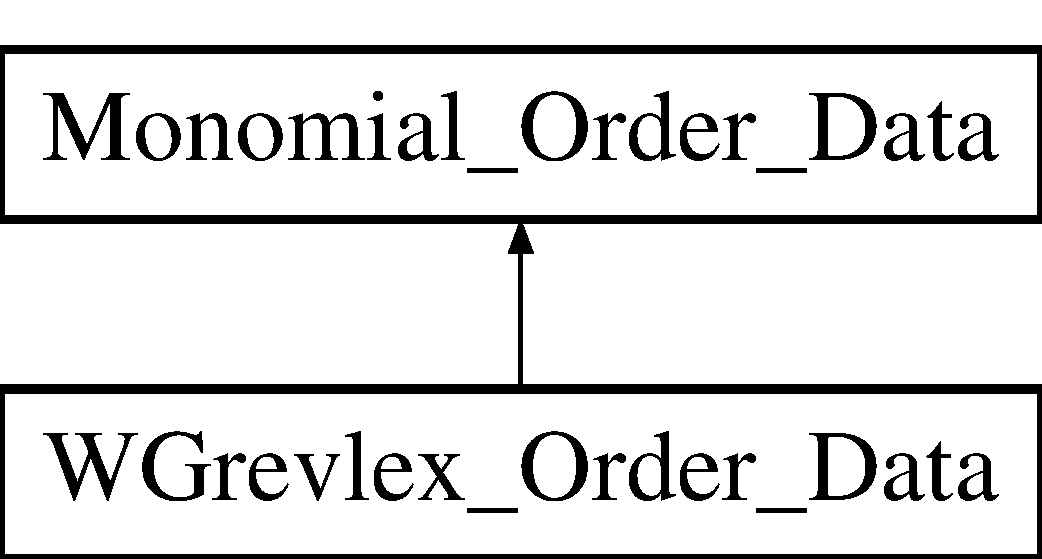
\includegraphics[height=2.000000cm]{group__orderinggroup}
\end{center}
\end{figure}
\subsubsection*{Public Member Functions}
\begin{Indent}\textbf{ Construction}\par
\begin{DoxyCompactItemize}
\item 
\hyperlink{group__orderinggroup_a35968aecc4009c0d15bfd357ccf74a5f}{Lex\+\_\+\+Ordering} (N\+V\+A\+R\+\_\+\+T\+Y\+PE number\+\_\+of\+\_\+variables)
\begin{DoxyCompactList}\small\item\em creates a lex ordering specific to $n$ variables \end{DoxyCompactList}\end{DoxyCompactItemize}
\end{Indent}
\begin{Indent}\textbf{ Comparison}\par
\begin{DoxyCompactItemize}
\item 
virtual bool \hyperlink{group__orderinggroup_acf085490051fdbbdde6e89831e3f0eda}{first\+\_\+larger} (const \hyperlink{group__polygroup_class_monomial}{Monomial} \&t, const \hyperlink{group__polygroup_class_monomial}{Monomial} \&u) const override
\item 
virtual bool \hyperlink{group__orderinggroup_ae42ea2c7b8fa45bcb46e56480d5f8abb}{first\+\_\+smaller} (const \hyperlink{group__polygroup_class_monomial}{Monomial} \&t, const \hyperlink{group__polygroup_class_monomial}{Monomial} \&u) const override
\item 
virtual bool \hyperlink{group__orderinggroup_a3ed34485d01b60236bc2ed70e05ed06a}{first\+\_\+larger\+\_\+than\+\_\+multiple} (const \hyperlink{group__polygroup_class_monomial}{Monomial} \&t, const \hyperlink{group__polygroup_class_monomial}{Monomial} \&u, const \hyperlink{group__polygroup_class_monomial}{Monomial} \&v) const override
\item 
virtual int \hyperlink{group__orderinggroup_a44d74f3b1e29abde22334f455979a67f}{cmp} (const \hyperlink{group__polygroup_class_monomial}{Monomial} \&t, const \hyperlink{group__polygroup_class_monomial}{Monomial} \&u) const override
\end{DoxyCompactItemize}
\end{Indent}
\subsubsection*{Protected Attributes}
\begin{DoxyCompactItemize}
\item 
\mbox{\Hypertarget{group__orderinggroup_a5065dfa6430e7fef522edbf762841ab7}\label{group__orderinggroup_a5065dfa6430e7fef522edbf762841ab7}} 
const N\+V\+A\+R\+\_\+\+T\+Y\+PE \hyperlink{group__orderinggroup_a5065dfa6430e7fef522edbf762841ab7}{n}
\begin{DoxyCompactList}\small\item\em the number of variables, which should remain constant \end{DoxyCompactList}\end{DoxyCompactItemize}


\paragraph{Constructor \& Destructor Documentation}
\mbox{\Hypertarget{group__orderinggroup_a35968aecc4009c0d15bfd357ccf74a5f}\label{group__orderinggroup_a35968aecc4009c0d15bfd357ccf74a5f}} 
\index{Lex\+\_\+\+Ordering@{Lex\+\_\+\+Ordering}!Lex\+\_\+\+Ordering@{Lex\+\_\+\+Ordering}}
\index{Lex\+\_\+\+Ordering@{Lex\+\_\+\+Ordering}!Lex\+\_\+\+Ordering@{Lex\+\_\+\+Ordering}}
\subparagraph{\texorpdfstring{Lex\+\_\+\+Ordering()}{Lex\_Ordering()}}
{\footnotesize\ttfamily Lex\+\_\+\+Ordering\+::\+Lex\+\_\+\+Ordering (\begin{DoxyParamCaption}\item[{N\+V\+A\+R\+\_\+\+T\+Y\+PE}]{number\+\_\+of\+\_\+variables }\end{DoxyParamCaption})}



creates a lex ordering specific to $n$ variables 


\begin{DoxyParams}{Parameters}
{\em number\+\_\+of\+\_\+variables} & number of variables this ordering should check \\
\hline
\end{DoxyParams}


Definition at line 337 of file particular\+\_\+orderings.\+cpp.



\paragraph{Member Function Documentation}
\mbox{\Hypertarget{group__orderinggroup_a44d74f3b1e29abde22334f455979a67f}\label{group__orderinggroup_a44d74f3b1e29abde22334f455979a67f}} 
\index{Lex\+\_\+\+Ordering@{Lex\+\_\+\+Ordering}!cmp@{cmp}}
\index{cmp@{cmp}!Lex\+\_\+\+Ordering@{Lex\+\_\+\+Ordering}}
\subparagraph{\texorpdfstring{cmp()}{cmp()}}
{\footnotesize\ttfamily virtual int Lex\+\_\+\+Ordering\+::cmp (\begin{DoxyParamCaption}\item[{const \hyperlink{group__polygroup_class_monomial}{Monomial} \&}]{t,  }\item[{const \hyperlink{group__polygroup_class_monomial}{Monomial} \&}]{u }\end{DoxyParamCaption}) const\hspace{0.3cm}{\ttfamily [inline]}, {\ttfamily [override]}, {\ttfamily [virtual]}}


\begin{DoxyParams}{Parameters}
{\em t} & a \hyperlink{group__polygroup_class_monomial}{Monomial}, to compare to $ u $ \\
\hline
{\em u} & a \hyperlink{group__polygroup_class_monomial}{Monomial}, to compare to $ t $ \\
\hline
\end{DoxyParams}
\begin{DoxyReturn}{Returns}
1 if $ t>u $ , -\/1 if $ t < u $ , and 0 otherwise 
\end{DoxyReturn}


Implements \hyperlink{group__orderinggroup_a9bc3155fc98b4d40c26118fa2114b827}{Monomial\+\_\+\+Ordering}.



Definition at line 377 of file particular\+\_\+orderings.\+hpp.

\mbox{\Hypertarget{group__orderinggroup_acf085490051fdbbdde6e89831e3f0eda}\label{group__orderinggroup_acf085490051fdbbdde6e89831e3f0eda}} 
\index{Lex\+\_\+\+Ordering@{Lex\+\_\+\+Ordering}!first\+\_\+larger@{first\+\_\+larger}}
\index{first\+\_\+larger@{first\+\_\+larger}!Lex\+\_\+\+Ordering@{Lex\+\_\+\+Ordering}}
\subparagraph{\texorpdfstring{first\+\_\+larger()}{first\_larger()}}
{\footnotesize\ttfamily bool Lex\+\_\+\+Ordering\+::first\+\_\+larger (\begin{DoxyParamCaption}\item[{const \hyperlink{group__polygroup_class_monomial}{Monomial} \&}]{t,  }\item[{const \hyperlink{group__polygroup_class_monomial}{Monomial} \&}]{u }\end{DoxyParamCaption}) const\hspace{0.3cm}{\ttfamily [override]}, {\ttfamily [virtual]}}

\begin{DoxyReturn}{Returns}
{\ttfamily true} iff $t>u$ 
\end{DoxyReturn}

\begin{DoxyParams}{Parameters}
{\em t} & a \hyperlink{group__polygroup_class_monomial}{Monomial}, to compare to $ u $ \\
\hline
{\em u} & a \hyperlink{group__polygroup_class_monomial}{Monomial}, to compare to $ t $ \\
\hline
\end{DoxyParams}


Implements \hyperlink{group__orderinggroup_aed41fe82e1ca5cd287a93d287fee7c20}{Monomial\+\_\+\+Ordering}.



Definition at line 340 of file particular\+\_\+orderings.\+cpp.

\mbox{\Hypertarget{group__orderinggroup_a3ed34485d01b60236bc2ed70e05ed06a}\label{group__orderinggroup_a3ed34485d01b60236bc2ed70e05ed06a}} 
\index{Lex\+\_\+\+Ordering@{Lex\+\_\+\+Ordering}!first\+\_\+larger\+\_\+than\+\_\+multiple@{first\+\_\+larger\+\_\+than\+\_\+multiple}}
\index{first\+\_\+larger\+\_\+than\+\_\+multiple@{first\+\_\+larger\+\_\+than\+\_\+multiple}!Lex\+\_\+\+Ordering@{Lex\+\_\+\+Ordering}}
\subparagraph{\texorpdfstring{first\+\_\+larger\+\_\+than\+\_\+multiple()}{first\_larger\_than\_multiple()}}
{\footnotesize\ttfamily bool Lex\+\_\+\+Ordering\+::first\+\_\+larger\+\_\+than\+\_\+multiple (\begin{DoxyParamCaption}\item[{const \hyperlink{group__polygroup_class_monomial}{Monomial} \&}]{t,  }\item[{const \hyperlink{group__polygroup_class_monomial}{Monomial} \&}]{u,  }\item[{const \hyperlink{group__polygroup_class_monomial}{Monomial} \&}]{v }\end{DoxyParamCaption}) const\hspace{0.3cm}{\ttfamily [override]}, {\ttfamily [virtual]}}


\begin{DoxyParams}{Parameters}
{\em t} & a \hyperlink{group__polygroup_class_monomial}{Monomial}, to compare to $ uv $ \\
\hline
{\em u} & a \hyperlink{group__polygroup_class_monomial}{Monomial}, to multiply to $ v $ \\
\hline
{\em v} & a \hyperlink{group__polygroup_class_monomial}{Monomial}, to multiply to $ u $ \\
\hline
\end{DoxyParams}
\begin{DoxyReturn}{Returns}
{\ttfamily true} iff $t>uv$ 
\end{DoxyReturn}


Implements \hyperlink{group__orderinggroup_aacb0439b908d45cc5f2635567c6633fd}{Monomial\+\_\+\+Ordering}.



Definition at line 372 of file particular\+\_\+orderings.\+cpp.

\mbox{\Hypertarget{group__orderinggroup_ae42ea2c7b8fa45bcb46e56480d5f8abb}\label{group__orderinggroup_ae42ea2c7b8fa45bcb46e56480d5f8abb}} 
\index{Lex\+\_\+\+Ordering@{Lex\+\_\+\+Ordering}!first\+\_\+smaller@{first\+\_\+smaller}}
\index{first\+\_\+smaller@{first\+\_\+smaller}!Lex\+\_\+\+Ordering@{Lex\+\_\+\+Ordering}}
\subparagraph{\texorpdfstring{first\+\_\+smaller()}{first\_smaller()}}
{\footnotesize\ttfamily bool Lex\+\_\+\+Ordering\+::first\+\_\+smaller (\begin{DoxyParamCaption}\item[{const \hyperlink{group__polygroup_class_monomial}{Monomial} \&}]{t,  }\item[{const \hyperlink{group__polygroup_class_monomial}{Monomial} \&}]{u }\end{DoxyParamCaption}) const\hspace{0.3cm}{\ttfamily [override]}, {\ttfamily [virtual]}}

\begin{DoxyReturn}{Returns}
{\ttfamily true} iff $t< u$ 
\end{DoxyReturn}

\begin{DoxyParams}{Parameters}
{\em t} & a \hyperlink{group__polygroup_class_monomial}{Monomial}, to compare to $ u $ \\
\hline
{\em u} & a \hyperlink{group__polygroup_class_monomial}{Monomial}, to compare to $ t $ \\
\hline
\end{DoxyParams}


Implements \hyperlink{group__orderinggroup_ab6c02638f87382f7a9a95b994e9a5dfb}{Monomial\+\_\+\+Ordering}.



Definition at line 356 of file particular\+\_\+orderings.\+cpp.

\index{Matrix\+\_\+\+Ordering@{Matrix\+\_\+\+Ordering}}\label{class_matrix___ordering}
\Hypertarget{group__orderinggroup_class_matrix___ordering}
\subsubsection{class Matrix\+\_\+\+Ordering}
orderings defined by a nonsingular matrix 

\begin{DoxyAuthor}{Author}
John Perry 
\end{DoxyAuthor}
\begin{DoxyDate}{Date}
2016 
\end{DoxyDate}


Definition at line 569 of file particular\+\_\+orderings.\+hpp.

Inheritance diagram for Matrix\+\_\+\+Ordering\+:\begin{figure}[H]
\begin{center}
\leavevmode
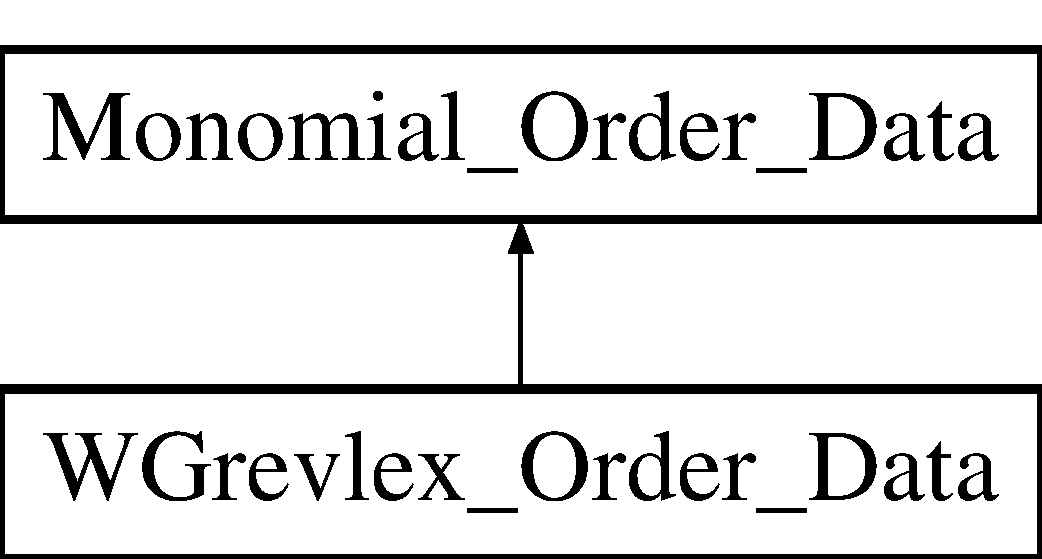
\includegraphics[height=2.000000cm]{group__orderinggroup}
\end{center}
\end{figure}
\subsubsection*{Public Member Functions}
\begin{DoxyCompactItemize}
\item 
\hyperlink{group__orderinggroup_a59c24eeefe79a784f51253dcd0a51101}{Matrix\+\_\+\+Ordering} (N\+V\+A\+R\+\_\+\+T\+Y\+PE rows, N\+V\+A\+R\+\_\+\+T\+Y\+PE cols, const W\+T\+\_\+\+T\+Y\+PE $\ast$$\ast$data)
\begin{DoxyCompactList}\small\item\em checks that {\ttfamily data} defines a nonsingular matrix, and sets things up \end{DoxyCompactList}\item 
virtual int \hyperlink{group__orderinggroup_a36f19a053b608126d1e35e62e6c35e35}{cmp} (const \hyperlink{group__polygroup_class_monomial}{Monomial} \&t, const \hyperlink{group__polygroup_class_monomial}{Monomial} \&u) const override
\item 
virtual bool \hyperlink{group__orderinggroup_aed327b2dfb248ac239694717c3313e31}{first\+\_\+larger} (const \hyperlink{group__polygroup_class_monomial}{Monomial} \&t, const \hyperlink{group__polygroup_class_monomial}{Monomial} \&u) const override
\item 
virtual bool \hyperlink{group__orderinggroup_ad9be3dafe786d480521cc0a31ebdef8c}{first\+\_\+larger\+\_\+than\+\_\+multiple} (const \hyperlink{group__polygroup_class_monomial}{Monomial} \&t, const \hyperlink{group__polygroup_class_monomial}{Monomial} \&u, const \hyperlink{group__polygroup_class_monomial}{Monomial} \&v) const override
\item 
virtual bool \hyperlink{group__orderinggroup_ab7881ff6bbc52d02bf786ef8ab8c5c37}{first\+\_\+smaller} (const \hyperlink{group__polygroup_class_monomial}{Monomial} \&t, const \hyperlink{group__polygroup_class_monomial}{Monomial} \&u) const override
\end{DoxyCompactItemize}
\subsubsection*{Protected Attributes}
\begin{DoxyCompactItemize}
\item 
\mbox{\Hypertarget{group__orderinggroup_a29f4b562f274f6bee1c3f3826a5d1cce}\label{group__orderinggroup_a29f4b562f274f6bee1c3f3826a5d1cce}} 
const N\+V\+A\+R\+\_\+\+T\+Y\+PE \hyperlink{group__orderinggroup_a29f4b562f274f6bee1c3f3826a5d1cce}{m}
\begin{DoxyCompactList}\small\item\em the number of rows \end{DoxyCompactList}\item 
\mbox{\Hypertarget{group__orderinggroup_a6508f4b4a5d5cac0da07ddea10c97d62}\label{group__orderinggroup_a6508f4b4a5d5cac0da07ddea10c97d62}} 
const N\+V\+A\+R\+\_\+\+T\+Y\+PE \hyperlink{group__orderinggroup_a6508f4b4a5d5cac0da07ddea10c97d62}{n}
\begin{DoxyCompactList}\small\item\em the number of columns \end{DoxyCompactList}\item 
\mbox{\Hypertarget{group__orderinggroup_a98a4930577909a94fb3b8ba734d0c2e2}\label{group__orderinggroup_a98a4930577909a94fb3b8ba734d0c2e2}} 
const W\+T\+\_\+\+T\+Y\+PE $\ast$$\ast$ \hyperlink{group__orderinggroup_a98a4930577909a94fb3b8ba734d0c2e2}{W}
\begin{DoxyCompactList}\small\item\em the matrix that defines this ordering \end{DoxyCompactList}\end{DoxyCompactItemize}


\paragraph{Constructor \& Destructor Documentation}
\mbox{\Hypertarget{group__orderinggroup_a59c24eeefe79a784f51253dcd0a51101}\label{group__orderinggroup_a59c24eeefe79a784f51253dcd0a51101}} 
\index{Matrix\+\_\+\+Ordering@{Matrix\+\_\+\+Ordering}!Matrix\+\_\+\+Ordering@{Matrix\+\_\+\+Ordering}}
\index{Matrix\+\_\+\+Ordering@{Matrix\+\_\+\+Ordering}!Matrix\+\_\+\+Ordering@{Matrix\+\_\+\+Ordering}}
\subparagraph{\texorpdfstring{Matrix\+\_\+\+Ordering()}{Matrix\_Ordering()}}
{\footnotesize\ttfamily Matrix\+\_\+\+Ordering\+::\+Matrix\+\_\+\+Ordering (\begin{DoxyParamCaption}\item[{N\+V\+A\+R\+\_\+\+T\+Y\+PE}]{rows,  }\item[{N\+V\+A\+R\+\_\+\+T\+Y\+PE}]{cols,  }\item[{const W\+T\+\_\+\+T\+Y\+PE $\ast$$\ast$}]{data }\end{DoxyParamCaption})}



checks that {\ttfamily data} defines a nonsingular matrix, and sets things up 


\begin{DoxyParams}{Parameters}
{\em rows} & number of rows desired in the matrix \\
\hline
{\em cols} & number of columns desired in the matrix \\
\hline
{\em data} & should contain $ rows \times cols $ elements \\
\hline
\end{DoxyParams}


Definition at line 628 of file particular\+\_\+orderings.\+cpp.



\paragraph{Member Function Documentation}
\mbox{\Hypertarget{group__orderinggroup_a36f19a053b608126d1e35e62e6c35e35}\label{group__orderinggroup_a36f19a053b608126d1e35e62e6c35e35}} 
\index{Matrix\+\_\+\+Ordering@{Matrix\+\_\+\+Ordering}!cmp@{cmp}}
\index{cmp@{cmp}!Matrix\+\_\+\+Ordering@{Matrix\+\_\+\+Ordering}}
\subparagraph{\texorpdfstring{cmp()}{cmp()}}
{\footnotesize\ttfamily virtual int Matrix\+\_\+\+Ordering\+::cmp (\begin{DoxyParamCaption}\item[{const \hyperlink{group__polygroup_class_monomial}{Monomial} \&}]{t,  }\item[{const \hyperlink{group__polygroup_class_monomial}{Monomial} \&}]{u }\end{DoxyParamCaption}) const\hspace{0.3cm}{\ttfamily [inline]}, {\ttfamily [override]}, {\ttfamily [virtual]}}


\begin{DoxyParams}{Parameters}
{\em t} & a \hyperlink{group__polygroup_class_monomial}{Monomial}, to compare to $ u $ \\
\hline
{\em u} & a \hyperlink{group__polygroup_class_monomial}{Monomial}, to compare to $ t $ \\
\hline
\end{DoxyParams}
\begin{DoxyReturn}{Returns}
1 if $ t>u $ , -\/1 if $ t < u $ , and 0 otherwise 
\end{DoxyReturn}


Implements \hyperlink{group__orderinggroup_a9bc3155fc98b4d40c26118fa2114b827}{Monomial\+\_\+\+Ordering}.



Definition at line 605 of file particular\+\_\+orderings.\+hpp.

\mbox{\Hypertarget{group__orderinggroup_aed327b2dfb248ac239694717c3313e31}\label{group__orderinggroup_aed327b2dfb248ac239694717c3313e31}} 
\index{Matrix\+\_\+\+Ordering@{Matrix\+\_\+\+Ordering}!first\+\_\+larger@{first\+\_\+larger}}
\index{first\+\_\+larger@{first\+\_\+larger}!Matrix\+\_\+\+Ordering@{Matrix\+\_\+\+Ordering}}
\subparagraph{\texorpdfstring{first\+\_\+larger()}{first\_larger()}}
{\footnotesize\ttfamily bool Matrix\+\_\+\+Ordering\+::first\+\_\+larger (\begin{DoxyParamCaption}\item[{const \hyperlink{group__polygroup_class_monomial}{Monomial} \&}]{t,  }\item[{const \hyperlink{group__polygroup_class_monomial}{Monomial} \&}]{u }\end{DoxyParamCaption}) const\hspace{0.3cm}{\ttfamily [override]}, {\ttfamily [virtual]}}


\begin{DoxyParams}{Parameters}
{\em t} & a \hyperlink{group__polygroup_class_monomial}{Monomial}, to compare to $ u $ \\
\hline
{\em u} & a \hyperlink{group__polygroup_class_monomial}{Monomial}, to compare to $ t $ \\
\hline
\end{DoxyParams}
\begin{DoxyReturn}{Returns}
{\ttfamily true} iff first \hyperlink{group__polygroup_class_monomial}{Monomial} is larger than second 
\end{DoxyReturn}


Implements \hyperlink{group__orderinggroup_aed41fe82e1ca5cd287a93d287fee7c20}{Monomial\+\_\+\+Ordering}.



Definition at line 635 of file particular\+\_\+orderings.\+cpp.

\mbox{\Hypertarget{group__orderinggroup_ad9be3dafe786d480521cc0a31ebdef8c}\label{group__orderinggroup_ad9be3dafe786d480521cc0a31ebdef8c}} 
\index{Matrix\+\_\+\+Ordering@{Matrix\+\_\+\+Ordering}!first\+\_\+larger\+\_\+than\+\_\+multiple@{first\+\_\+larger\+\_\+than\+\_\+multiple}}
\index{first\+\_\+larger\+\_\+than\+\_\+multiple@{first\+\_\+larger\+\_\+than\+\_\+multiple}!Matrix\+\_\+\+Ordering@{Matrix\+\_\+\+Ordering}}
\subparagraph{\texorpdfstring{first\+\_\+larger\+\_\+than\+\_\+multiple()}{first\_larger\_than\_multiple()}}
{\footnotesize\ttfamily bool Matrix\+\_\+\+Ordering\+::first\+\_\+larger\+\_\+than\+\_\+multiple (\begin{DoxyParamCaption}\item[{const \hyperlink{group__polygroup_class_monomial}{Monomial} \&}]{t,  }\item[{const \hyperlink{group__polygroup_class_monomial}{Monomial} \&}]{u,  }\item[{const \hyperlink{group__polygroup_class_monomial}{Monomial} \&}]{v }\end{DoxyParamCaption}) const\hspace{0.3cm}{\ttfamily [override]}, {\ttfamily [virtual]}}


\begin{DoxyParams}{Parameters}
{\em t} & a \hyperlink{group__polygroup_class_monomial}{Monomial}, to compare to $ uv $ \\
\hline
{\em u} & a \hyperlink{group__polygroup_class_monomial}{Monomial}, to multiply to $ v $ \\
\hline
{\em v} & a \hyperlink{group__polygroup_class_monomial}{Monomial}, to multiply to $ u $ \\
\hline
\end{DoxyParams}
\begin{DoxyReturn}{Returns}
{\ttfamily true} iff first \hyperlink{group__polygroup_class_monomial}{Monomial} is larger than product of second and third 
\end{DoxyReturn}


Implements \hyperlink{group__orderinggroup_aacb0439b908d45cc5f2635567c6633fd}{Monomial\+\_\+\+Ordering}.



Definition at line 681 of file particular\+\_\+orderings.\+cpp.

\mbox{\Hypertarget{group__orderinggroup_ab7881ff6bbc52d02bf786ef8ab8c5c37}\label{group__orderinggroup_ab7881ff6bbc52d02bf786ef8ab8c5c37}} 
\index{Matrix\+\_\+\+Ordering@{Matrix\+\_\+\+Ordering}!first\+\_\+smaller@{first\+\_\+smaller}}
\index{first\+\_\+smaller@{first\+\_\+smaller}!Matrix\+\_\+\+Ordering@{Matrix\+\_\+\+Ordering}}
\subparagraph{\texorpdfstring{first\+\_\+smaller()}{first\_smaller()}}
{\footnotesize\ttfamily bool Matrix\+\_\+\+Ordering\+::first\+\_\+smaller (\begin{DoxyParamCaption}\item[{const \hyperlink{group__polygroup_class_monomial}{Monomial} \&}]{t,  }\item[{const \hyperlink{group__polygroup_class_monomial}{Monomial} \&}]{u }\end{DoxyParamCaption}) const\hspace{0.3cm}{\ttfamily [override]}, {\ttfamily [virtual]}}


\begin{DoxyParams}{Parameters}
{\em t} & a \hyperlink{group__polygroup_class_monomial}{Monomial}, to compare to $ u $ \\
\hline
{\em u} & a \hyperlink{group__polygroup_class_monomial}{Monomial}, to compare to $ t $ \\
\hline
\end{DoxyParams}
\begin{DoxyReturn}{Returns}
{\ttfamily true} iff first \hyperlink{group__polygroup_class_monomial}{Monomial} is smaller than second 
\end{DoxyReturn}


Implements \hyperlink{group__orderinggroup_ab6c02638f87382f7a9a95b994e9a5dfb}{Monomial\+\_\+\+Ordering}.



Definition at line 658 of file particular\+\_\+orderings.\+cpp.

\index{Monomial\+\_\+\+Order\+\_\+\+Data@{Monomial\+\_\+\+Order\+\_\+\+Data}}\label{class_monomial___order___data}
\Hypertarget{group__orderinggroup_class_monomial___order___data}
\subsubsection{class Monomial\+\_\+\+Order\+\_\+\+Data}
data for a monomial ordering\+: optional, but stored in {\ttfamily \hyperlink{group__polygroup_class_monomial}{Monomial}} 

\begin{DoxyAuthor}{Author}
John Perry 
\end{DoxyAuthor}
\begin{DoxyDate}{Date}
2015 
\end{DoxyDate}


Definition at line 39 of file monomial\+\_\+ordering.\+hpp.

Inheritance diagram for Monomial\+\_\+\+Order\+\_\+\+Data\+:\begin{figure}[H]
\begin{center}
\leavevmode
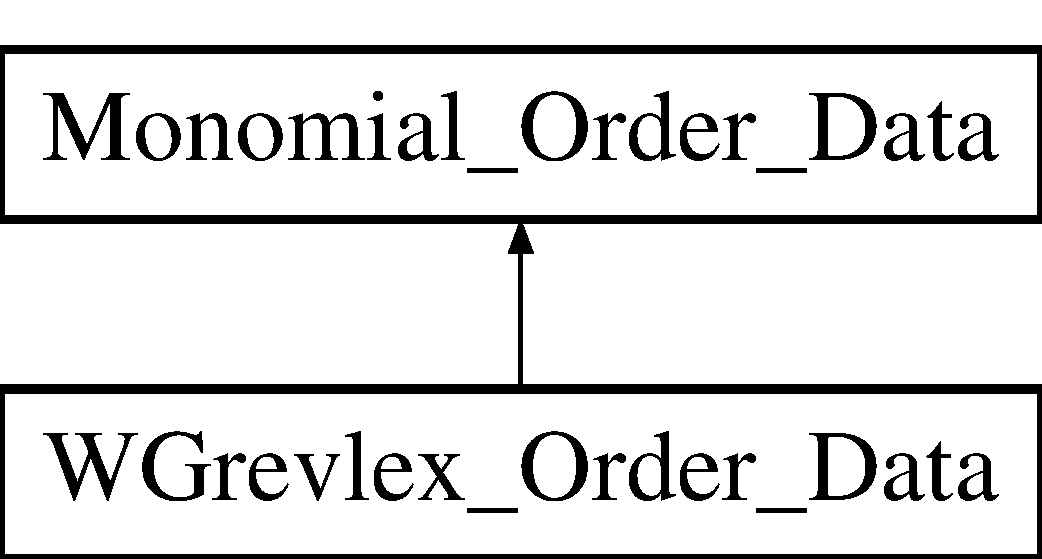
\includegraphics[height=2.000000cm]{group__orderinggroup}
\end{center}
\end{figure}
\subsubsection*{Public Member Functions}
\begin{Indent}\textbf{ Construction}\par
\begin{DoxyCompactItemize}
\item 
\mbox{\Hypertarget{group__orderinggroup_a636a75b3d5e776f9ed09668a3b9673c6}\label{group__orderinggroup_a636a75b3d5e776f9ed09668a3b9673c6}} 
virtual \hyperlink{group__orderinggroup_class_monomial___order___data}{Monomial\+\_\+\+Order\+\_\+\+Data} $\ast$ \hyperlink{group__orderinggroup_a636a75b3d5e776f9ed09668a3b9673c6}{clone} ()
\begin{DoxyCompactList}\small\item\em default clone returns {\ttfamily nullptr} \end{DoxyCompactList}\end{DoxyCompactItemize}
\end{Indent}
\begin{Indent}\textbf{ Basic data}\par
\begin{DoxyCompactItemize}
\item 
\mbox{\Hypertarget{group__orderinggroup_a581ab0398e12b7c0ad80212ad50e86b8}\label{group__orderinggroup_a581ab0398e12b7c0ad80212ad50e86b8}} 
virtual D\+E\+G\+\_\+\+T\+Y\+PE \hyperlink{group__orderinggroup_a581ab0398e12b7c0ad80212ad50e86b8}{grading} (N\+V\+A\+R\+\_\+\+T\+Y\+PE) const
\begin{DoxyCompactList}\small\item\em default value is useless; orderings that supply gradings should redefine \end{DoxyCompactList}\end{DoxyCompactItemize}
\end{Indent}
\begin{Indent}\textbf{ Destruction}\par
\begin{DoxyCompactItemize}
\item 
\mbox{\Hypertarget{group__orderinggroup_a278b8c06b208d8549ba2f871f93239be}\label{group__orderinggroup_a278b8c06b208d8549ba2f871f93239be}} 
virtual \hyperlink{group__orderinggroup_a278b8c06b208d8549ba2f871f93239be}{$\sim$\+Monomial\+\_\+\+Order\+\_\+\+Data} ()
\begin{DoxyCompactList}\small\item\em does nothing but guarantee polymorphism (stupid, stupid C++) \end{DoxyCompactList}\end{DoxyCompactItemize}
\end{Indent}
\index{Monomial\+\_\+\+Ordering@{Monomial\+\_\+\+Ordering}}\label{class_monomial___ordering}
\Hypertarget{group__orderinggroup_class_monomial___ordering}
\subsubsection{class Monomial\+\_\+\+Ordering}
interface to a monomial ordering 

\begin{DoxyAuthor}{Author}
John Perry 
\end{DoxyAuthor}
\begin{DoxyDate}{Date}
2015 
\end{DoxyDate}
\begin{DoxyWarning}{Warning}
Avoid changing the monomial ordering data in the comparison functions, as the user may wish to compare two monomials according to a different ordering than the current value. This is the reason those functions are marked to leave the Monomials constant. The expected behavior is that \hyperlink{group__orderinggroup_aed41fe82e1ca5cd287a93d287fee7c20}{first\+\_\+larger()} does whatever the ordering wants, so if you need monomial data check first to decide whether it exists, and applies to this ordering! Use \hyperlink{group__orderinggroup_a22b08dffd1cdf3a655ca18d604cfcee1}{set\+\_\+data()} if you want to change the monomials first.

There is no strict need to check whether the monomials are associated to the same ordering, but if the ordering uses \hyperlink{group__orderinggroup_class_monomial___order___data}{Monomial\+\_\+\+Order\+\_\+\+Data} one would be foolhardy not to check first. 
\end{DoxyWarning}
\begin{Desc}
\item[Examples\+: ]\par
\hyperlink{test_cyclicn_8cpp-example}{test\+\_\+cyclicn.\+cpp}, and \hyperlink{test_dynamic_8cpp-example}{test\+\_\+dynamic.\+cpp}.\end{Desc}


Definition at line 77 of file monomial\+\_\+ordering.\+hpp.

Inheritance diagram for Monomial\+\_\+\+Ordering\+:\begin{figure}[H]
\begin{center}
\leavevmode
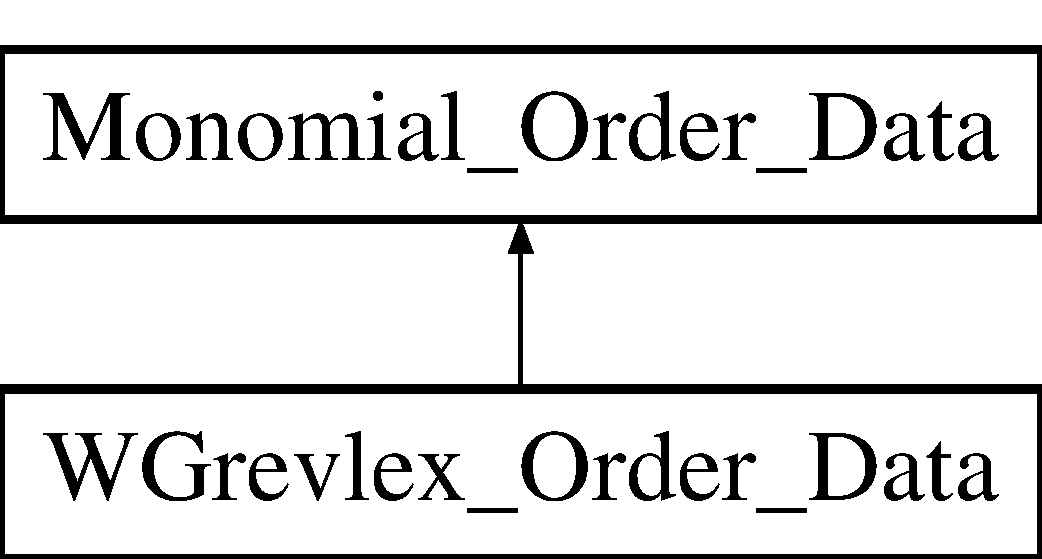
\includegraphics[height=1.581921cm]{group__orderinggroup}
\end{center}
\end{figure}
\subsubsection*{Public Member Functions}
\begin{Indent}\textbf{ Destruction}\par
\begin{DoxyCompactItemize}
\item 
\mbox{\Hypertarget{group__orderinggroup_a6f507bd325e959ce867880d4696a99cc}\label{group__orderinggroup_a6f507bd325e959ce867880d4696a99cc}} 
virtual \hyperlink{group__orderinggroup_a6f507bd325e959ce867880d4696a99cc}{$\sim$\+Monomial\+\_\+\+Ordering} ()
\begin{DoxyCompactList}\small\item\em needs virtual destructor for polymorphic {\ttfamily delete} \end{DoxyCompactList}\end{DoxyCompactItemize}
\end{Indent}
\begin{Indent}\textbf{ Utility}\par
\begin{DoxyCompactItemize}
\item 
virtual void \hyperlink{group__orderinggroup_a22b08dffd1cdf3a655ca18d604cfcee1}{set\+\_\+data} (\hyperlink{group__polygroup_class_monomial}{Monomial} \&) const
\begin{DoxyCompactList}\small\item\em sets monomial ordering's data; default is to do nothing \end{DoxyCompactList}\end{DoxyCompactItemize}
\end{Indent}
\begin{Indent}\textbf{ Comparison}\par
\begin{DoxyCompactItemize}
\item 
virtual int \hyperlink{group__orderinggroup_a9bc3155fc98b4d40c26118fa2114b827}{cmp} (const \hyperlink{group__polygroup_class_monomial}{Monomial} \&t, const \hyperlink{group__polygroup_class_monomial}{Monomial} \&u) const =0
\begin{DoxyCompactList}\small\item\em \{@ \end{DoxyCompactList}\item 
virtual bool \hyperlink{group__orderinggroup_aed41fe82e1ca5cd287a93d287fee7c20}{first\+\_\+larger} (const \hyperlink{group__polygroup_class_monomial}{Monomial} \&, const \hyperlink{group__polygroup_class_monomial}{Monomial} \&) const =0
\item 
bool \hyperlink{group__orderinggroup_afbae8e00a02ce0334bb0376cf0f0db75}{first\+\_\+larger\+\_\+or\+\_\+equal} (const \hyperlink{group__polygroup_class_monomial}{Monomial} \&, const \hyperlink{group__polygroup_class_monomial}{Monomial} \&) const
\item 
virtual bool \hyperlink{group__orderinggroup_ab6c02638f87382f7a9a95b994e9a5dfb}{first\+\_\+smaller} (const \hyperlink{group__polygroup_class_monomial}{Monomial} \&, const \hyperlink{group__polygroup_class_monomial}{Monomial} \&) const =0
\item 
bool \hyperlink{group__orderinggroup_ac9234fccc26cca2aee57e28af7b61880}{first\+\_\+smaller\+\_\+or\+\_\+equal} (const \hyperlink{group__polygroup_class_monomial}{Monomial} \&, const \hyperlink{group__polygroup_class_monomial}{Monomial} \&) const
\item 
\mbox{\Hypertarget{group__orderinggroup_aacb0439b908d45cc5f2635567c6633fd}\label{group__orderinggroup_aacb0439b908d45cc5f2635567c6633fd}} 
virtual bool \hyperlink{group__orderinggroup_aacb0439b908d45cc5f2635567c6633fd}{first\+\_\+larger\+\_\+than\+\_\+multiple} (const \hyperlink{group__polygroup_class_monomial}{Monomial} \&, const \hyperlink{group__polygroup_class_monomial}{Monomial} \&, const \hyperlink{group__polygroup_class_monomial}{Monomial} \&) const =0
\begin{DoxyCompactList}\small\item\em returns {\ttfamily true} iff the first \hyperlink{group__polygroup_class_monomial}{Monomial} is larger than the specified multiple of the second \end{DoxyCompactList}\item 
bool \hyperlink{group__orderinggroup_ad4af4c79cf46666222fe30fdd4ceb45e}{first\+\_\+larger\+\_\+or\+\_\+equal\+\_\+than\+\_\+multiple} (const \hyperlink{group__polygroup_class_monomial}{Monomial} \&, const \hyperlink{group__polygroup_class_monomial}{Monomial} \&, const \hyperlink{group__polygroup_class_monomial}{Monomial} \&) const
\item 
bool \hyperlink{group__orderinggroup_aad1ca67ca89fa85e63475d24d9f0a987}{first\+\_\+smaller\+\_\+than\+\_\+multiple} (const \hyperlink{group__polygroup_class_monomial}{Monomial} \&, const \hyperlink{group__polygroup_class_monomial}{Monomial} \&, const \hyperlink{group__polygroup_class_monomial}{Monomial} \&) const
\item 
bool \hyperlink{group__orderinggroup_a0ed5bf2b1da5daaa67aaba00f8c6cbd0}{first\+\_\+smaller\+\_\+or\+\_\+equal\+\_\+than\+\_\+multiple} (const \hyperlink{group__polygroup_class_monomial}{Monomial} \&, const \hyperlink{group__polygroup_class_monomial}{Monomial} \&, const \hyperlink{group__polygroup_class_monomial}{Monomial} \&) const
\end{DoxyCompactItemize}
\end{Indent}


\paragraph{Member Function Documentation}
\mbox{\Hypertarget{group__orderinggroup_a9bc3155fc98b4d40c26118fa2114b827}\label{group__orderinggroup_a9bc3155fc98b4d40c26118fa2114b827}} 
\index{Monomial\+\_\+\+Ordering@{Monomial\+\_\+\+Ordering}!cmp@{cmp}}
\index{cmp@{cmp}!Monomial\+\_\+\+Ordering@{Monomial\+\_\+\+Ordering}}
\subparagraph{\texorpdfstring{cmp()}{cmp()}}
{\footnotesize\ttfamily virtual int Monomial\+\_\+\+Ordering\+::cmp (\begin{DoxyParamCaption}\item[{const \hyperlink{group__polygroup_class_monomial}{Monomial} \&}]{t,  }\item[{const \hyperlink{group__polygroup_class_monomial}{Monomial} \&}]{u }\end{DoxyParamCaption}) const\hspace{0.3cm}{\ttfamily [pure virtual]}}



\{@ 


\begin{DoxyParams}{Parameters}
{\em t} & a \hyperlink{group__polygroup_class_monomial}{Monomial} to compare to $ u $ \\
\hline
{\em u} & a \hyperlink{group__polygroup_class_monomial}{Monomial} to compare to $ t $ \\
\hline
\end{DoxyParams}
\begin{DoxyReturn}{Returns}
0 if the Monomials are like; negative if smaller, positive if larger -- for efficiency, you probably want to redefine this 
\end{DoxyReturn}


Implemented in \hyperlink{group__orderinggroup_a36f19a053b608126d1e35e62e6c35e35}{Matrix\+\_\+\+Ordering}, \hyperlink{group__orderinggroup_afcba2ade4149724f666064643e502769}{Cached\+W\+Grevlex\+\_\+\+Ordering}, \hyperlink{group__orderinggroup_a44d74f3b1e29abde22334f455979a67f}{Lex\+\_\+\+Ordering}, \hyperlink{group__orderinggroup_a0a65b26c9057d7f9d8c29ca3896cfd74}{W\+Grevlex}, \hyperlink{group__orderinggroup_a1b668700d9ccc218ebae6049bb76fb07}{Grevlex\+\_\+\+Ordering}, and \hyperlink{group__orderinggroup_ae7103c92d45f749eaf3c5403b17a2828}{Generic\+\_\+\+Grevlex}.

\mbox{\Hypertarget{group__orderinggroup_aed41fe82e1ca5cd287a93d287fee7c20}\label{group__orderinggroup_aed41fe82e1ca5cd287a93d287fee7c20}} 
\index{Monomial\+\_\+\+Ordering@{Monomial\+\_\+\+Ordering}!first\+\_\+larger@{first\+\_\+larger}}
\index{first\+\_\+larger@{first\+\_\+larger}!Monomial\+\_\+\+Ordering@{Monomial\+\_\+\+Ordering}}
\subparagraph{\texorpdfstring{first\+\_\+larger()}{first\_larger()}}
{\footnotesize\ttfamily virtual bool Monomial\+\_\+\+Ordering\+::first\+\_\+larger (\begin{DoxyParamCaption}\item[{const \hyperlink{group__polygroup_class_monomial}{Monomial} \&}]{,  }\item[{const \hyperlink{group__polygroup_class_monomial}{Monomial} \&}]{ }\end{DoxyParamCaption}) const\hspace{0.3cm}{\ttfamily [pure virtual]}}

\begin{DoxyReturn}{Returns}
{\ttfamily true} iff the first \hyperlink{group__polygroup_class_monomial}{Monomial} is larger than the second 
\end{DoxyReturn}


Implemented in \hyperlink{group__orderinggroup_aed327b2dfb248ac239694717c3313e31}{Matrix\+\_\+\+Ordering}, \hyperlink{group__orderinggroup_a78e346a28a1dde835e487c01c7ce2b5a}{Cached\+W\+Grevlex\+\_\+\+Ordering}, \hyperlink{group__orderinggroup_acf085490051fdbbdde6e89831e3f0eda}{Lex\+\_\+\+Ordering}, \hyperlink{group__orderinggroup_a547c267540f69917cadbeba621642f2a}{W\+Grevlex}, \hyperlink{group__orderinggroup_a7ed2a24b293d63e26c0cdbe4270682a8}{Grevlex\+\_\+\+Ordering}, and \hyperlink{group__orderinggroup_ac412c73e940b4aabe1e350d6c98a99f5}{Generic\+\_\+\+Grevlex}.

\mbox{\Hypertarget{group__orderinggroup_afbae8e00a02ce0334bb0376cf0f0db75}\label{group__orderinggroup_afbae8e00a02ce0334bb0376cf0f0db75}} 
\index{Monomial\+\_\+\+Ordering@{Monomial\+\_\+\+Ordering}!first\+\_\+larger\+\_\+or\+\_\+equal@{first\+\_\+larger\+\_\+or\+\_\+equal}}
\index{first\+\_\+larger\+\_\+or\+\_\+equal@{first\+\_\+larger\+\_\+or\+\_\+equal}!Monomial\+\_\+\+Ordering@{Monomial\+\_\+\+Ordering}}
\subparagraph{\texorpdfstring{first\+\_\+larger\+\_\+or\+\_\+equal()}{first\_larger\_or\_equal()}}
{\footnotesize\ttfamily bool Monomial\+\_\+\+Ordering\+::first\+\_\+larger\+\_\+or\+\_\+equal (\begin{DoxyParamCaption}\item[{const \hyperlink{group__polygroup_class_monomial}{Monomial} \&}]{t,  }\item[{const \hyperlink{group__polygroup_class_monomial}{Monomial} \&}]{u }\end{DoxyParamCaption}) const}

\begin{DoxyReturn}{Returns}
{\ttfamily true} iff the first \hyperlink{group__polygroup_class_monomial}{Monomial} is larger or equal to the second 
\end{DoxyReturn}
\begin{DoxySeeAlso}{See also}
\hyperlink{group__orderinggroup_aed41fe82e1ca5cd287a93d287fee7c20}{first\+\_\+larger()} 
\end{DoxySeeAlso}
\begin{DoxyWarning}{Warning}
Do not override unless you know what you're doing 
\end{DoxyWarning}


Definition at line 490 of file monomial.\+cpp.

\mbox{\Hypertarget{group__orderinggroup_ad4af4c79cf46666222fe30fdd4ceb45e}\label{group__orderinggroup_ad4af4c79cf46666222fe30fdd4ceb45e}} 
\index{Monomial\+\_\+\+Ordering@{Monomial\+\_\+\+Ordering}!first\+\_\+larger\+\_\+or\+\_\+equal\+\_\+than\+\_\+multiple@{first\+\_\+larger\+\_\+or\+\_\+equal\+\_\+than\+\_\+multiple}}
\index{first\+\_\+larger\+\_\+or\+\_\+equal\+\_\+than\+\_\+multiple@{first\+\_\+larger\+\_\+or\+\_\+equal\+\_\+than\+\_\+multiple}!Monomial\+\_\+\+Ordering@{Monomial\+\_\+\+Ordering}}
\subparagraph{\texorpdfstring{first\+\_\+larger\+\_\+or\+\_\+equal\+\_\+than\+\_\+multiple()}{first\_larger\_or\_equal\_than\_multiple()}}
{\footnotesize\ttfamily bool Monomial\+\_\+\+Ordering\+::first\+\_\+larger\+\_\+or\+\_\+equal\+\_\+than\+\_\+multiple (\begin{DoxyParamCaption}\item[{const \hyperlink{group__polygroup_class_monomial}{Monomial} \&}]{t,  }\item[{const \hyperlink{group__polygroup_class_monomial}{Monomial} \&}]{u,  }\item[{const \hyperlink{group__polygroup_class_monomial}{Monomial} \&}]{v }\end{DoxyParamCaption}) const}

\begin{DoxyReturn}{Returns}
{\ttfamily true} iff the first \hyperlink{group__polygroup_class_monomial}{Monomial} is larger or equal to the specified multiple of the second 
\end{DoxyReturn}
\begin{DoxySeeAlso}{See also}
\hyperlink{group__orderinggroup_aed41fe82e1ca5cd287a93d287fee7c20}{first\+\_\+larger()} 
\end{DoxySeeAlso}
\begin{DoxyWarning}{Warning}
Do not override unless you know what you're doing 
\end{DoxyWarning}


Definition at line 496 of file monomial.\+cpp.

\mbox{\Hypertarget{group__orderinggroup_ab6c02638f87382f7a9a95b994e9a5dfb}\label{group__orderinggroup_ab6c02638f87382f7a9a95b994e9a5dfb}} 
\index{Monomial\+\_\+\+Ordering@{Monomial\+\_\+\+Ordering}!first\+\_\+smaller@{first\+\_\+smaller}}
\index{first\+\_\+smaller@{first\+\_\+smaller}!Monomial\+\_\+\+Ordering@{Monomial\+\_\+\+Ordering}}
\subparagraph{\texorpdfstring{first\+\_\+smaller()}{first\_smaller()}}
{\footnotesize\ttfamily virtual bool Monomial\+\_\+\+Ordering\+::first\+\_\+smaller (\begin{DoxyParamCaption}\item[{const \hyperlink{group__polygroup_class_monomial}{Monomial} \&}]{,  }\item[{const \hyperlink{group__polygroup_class_monomial}{Monomial} \&}]{ }\end{DoxyParamCaption}) const\hspace{0.3cm}{\ttfamily [pure virtual]}}

\begin{DoxyReturn}{Returns}
{\ttfamily true} iff the first \hyperlink{group__polygroup_class_monomial}{Monomial} is smaller than the second 
\end{DoxyReturn}
\begin{DoxyWarning}{Warning}
Do not override unless you know what you're doing 
\end{DoxyWarning}


Implemented in \hyperlink{group__orderinggroup_ab7881ff6bbc52d02bf786ef8ab8c5c37}{Matrix\+\_\+\+Ordering}, \hyperlink{group__orderinggroup_a131b09d8226c2dc5f0718f90ab8e009f}{Cached\+W\+Grevlex\+\_\+\+Ordering}, \hyperlink{group__orderinggroup_ae42ea2c7b8fa45bcb46e56480d5f8abb}{Lex\+\_\+\+Ordering}, \hyperlink{group__orderinggroup_a0e4327be4c18de7180ba2cd8c2f9d549}{W\+Grevlex}, \hyperlink{group__orderinggroup_abb1afdfa6ace5b90e425d0645e278c67}{Grevlex\+\_\+\+Ordering}, and \hyperlink{group__orderinggroup_a48ba39468e17d826988b28f5d871d868}{Generic\+\_\+\+Grevlex}.

\mbox{\Hypertarget{group__orderinggroup_ac9234fccc26cca2aee57e28af7b61880}\label{group__orderinggroup_ac9234fccc26cca2aee57e28af7b61880}} 
\index{Monomial\+\_\+\+Ordering@{Monomial\+\_\+\+Ordering}!first\+\_\+smaller\+\_\+or\+\_\+equal@{first\+\_\+smaller\+\_\+or\+\_\+equal}}
\index{first\+\_\+smaller\+\_\+or\+\_\+equal@{first\+\_\+smaller\+\_\+or\+\_\+equal}!Monomial\+\_\+\+Ordering@{Monomial\+\_\+\+Ordering}}
\subparagraph{\texorpdfstring{first\+\_\+smaller\+\_\+or\+\_\+equal()}{first\_smaller\_or\_equal()}}
{\footnotesize\ttfamily bool Monomial\+\_\+\+Ordering\+::first\+\_\+smaller\+\_\+or\+\_\+equal (\begin{DoxyParamCaption}\item[{const \hyperlink{group__polygroup_class_monomial}{Monomial} \&}]{t,  }\item[{const \hyperlink{group__polygroup_class_monomial}{Monomial} \&}]{u }\end{DoxyParamCaption}) const}

\begin{DoxyReturn}{Returns}
{\ttfamily true} iff the first \hyperlink{group__polygroup_class_monomial}{Monomial} is smaller or equal to the second 
\end{DoxyReturn}
\begin{DoxySeeAlso}{See also}
\hyperlink{group__orderinggroup_aed41fe82e1ca5cd287a93d287fee7c20}{first\+\_\+larger()} 
\end{DoxySeeAlso}
\begin{DoxyWarning}{Warning}
Do not override unless you know what you're doing 
\end{DoxyWarning}


Definition at line 30 of file monomial\+\_\+ordering.\+cpp.

\mbox{\Hypertarget{group__orderinggroup_a0ed5bf2b1da5daaa67aaba00f8c6cbd0}\label{group__orderinggroup_a0ed5bf2b1da5daaa67aaba00f8c6cbd0}} 
\index{Monomial\+\_\+\+Ordering@{Monomial\+\_\+\+Ordering}!first\+\_\+smaller\+\_\+or\+\_\+equal\+\_\+than\+\_\+multiple@{first\+\_\+smaller\+\_\+or\+\_\+equal\+\_\+than\+\_\+multiple}}
\index{first\+\_\+smaller\+\_\+or\+\_\+equal\+\_\+than\+\_\+multiple@{first\+\_\+smaller\+\_\+or\+\_\+equal\+\_\+than\+\_\+multiple}!Monomial\+\_\+\+Ordering@{Monomial\+\_\+\+Ordering}}
\subparagraph{\texorpdfstring{first\+\_\+smaller\+\_\+or\+\_\+equal\+\_\+than\+\_\+multiple()}{first\_smaller\_or\_equal\_than\_multiple()}}
{\footnotesize\ttfamily bool Monomial\+\_\+\+Ordering\+::first\+\_\+smaller\+\_\+or\+\_\+equal\+\_\+than\+\_\+multiple (\begin{DoxyParamCaption}\item[{const \hyperlink{group__polygroup_class_monomial}{Monomial} \&}]{t,  }\item[{const \hyperlink{group__polygroup_class_monomial}{Monomial} \&}]{u,  }\item[{const \hyperlink{group__polygroup_class_monomial}{Monomial} \&}]{v }\end{DoxyParamCaption}) const}

\begin{DoxyReturn}{Returns}
{\ttfamily true} iff the first \hyperlink{group__polygroup_class_monomial}{Monomial} is smaller or equal to the specified multiple of the second 
\end{DoxyReturn}
\begin{DoxySeeAlso}{See also}
\hyperlink{group__orderinggroup_aed41fe82e1ca5cd287a93d287fee7c20}{first\+\_\+larger()} 
\end{DoxySeeAlso}
\begin{DoxyWarning}{Warning}
Do not override unless you know what you're doing 
\end{DoxyWarning}


Definition at line 42 of file monomial\+\_\+ordering.\+cpp.

\mbox{\Hypertarget{group__orderinggroup_aad1ca67ca89fa85e63475d24d9f0a987}\label{group__orderinggroup_aad1ca67ca89fa85e63475d24d9f0a987}} 
\index{Monomial\+\_\+\+Ordering@{Monomial\+\_\+\+Ordering}!first\+\_\+smaller\+\_\+than\+\_\+multiple@{first\+\_\+smaller\+\_\+than\+\_\+multiple}}
\index{first\+\_\+smaller\+\_\+than\+\_\+multiple@{first\+\_\+smaller\+\_\+than\+\_\+multiple}!Monomial\+\_\+\+Ordering@{Monomial\+\_\+\+Ordering}}
\subparagraph{\texorpdfstring{first\+\_\+smaller\+\_\+than\+\_\+multiple()}{first\_smaller\_than\_multiple()}}
{\footnotesize\ttfamily bool Monomial\+\_\+\+Ordering\+::first\+\_\+smaller\+\_\+than\+\_\+multiple (\begin{DoxyParamCaption}\item[{const \hyperlink{group__polygroup_class_monomial}{Monomial} \&}]{t,  }\item[{const \hyperlink{group__polygroup_class_monomial}{Monomial} \&}]{u,  }\item[{const \hyperlink{group__polygroup_class_monomial}{Monomial} \&}]{v }\end{DoxyParamCaption}) const}

\begin{DoxyReturn}{Returns}
{\ttfamily true} iff the first \hyperlink{group__polygroup_class_monomial}{Monomial} is smaller than the specified multiple of the second 
\end{DoxyReturn}
\begin{DoxyWarning}{Warning}
Do not override unless you know what you're doing 
\end{DoxyWarning}


Definition at line 36 of file monomial\+\_\+ordering.\+cpp.

\mbox{\Hypertarget{group__orderinggroup_a22b08dffd1cdf3a655ca18d604cfcee1}\label{group__orderinggroup_a22b08dffd1cdf3a655ca18d604cfcee1}} 
\index{Monomial\+\_\+\+Ordering@{Monomial\+\_\+\+Ordering}!set\+\_\+data@{set\+\_\+data}}
\index{set\+\_\+data@{set\+\_\+data}!Monomial\+\_\+\+Ordering@{Monomial\+\_\+\+Ordering}}
\subparagraph{\texorpdfstring{set\+\_\+data()}{set\_data()}}
{\footnotesize\ttfamily void Monomial\+\_\+\+Ordering\+::set\+\_\+data (\begin{DoxyParamCaption}\item[{\hyperlink{group__polygroup_class_monomial}{Monomial} \&}]{t }\end{DoxyParamCaption}) const\hspace{0.3cm}{\ttfamily [virtual]}}



sets monomial ordering's data; default is to do nothing 

Child classes that override this function are strongly recommended to use set\+\_\+ordering\+\_\+degree() of the \hyperlink{group__polygroup_class_monomial}{Monomial} class to set a primary degree. For weighted/graded degree orderings, this typically improves performance nontrivially. 

Reimplemented in \hyperlink{group__orderinggroup_a65f1e27ee52413c91ffcb87632dcb27c}{Cached\+W\+Grevlex\+\_\+\+Ordering}, \hyperlink{group__orderinggroup_a18ba60cd0a76da002303a11d362142d9}{W\+Grevlex}, \hyperlink{group__orderinggroup_a83abd3e7505fe2096b01b8146bfdd83f}{Grevlex\+\_\+\+Ordering}, and \hyperlink{group__orderinggroup_a14c344858da03d16c8019afdae3da5dc}{Generic\+\_\+\+Grevlex}.



Definition at line 486 of file monomial.\+cpp.

\index{Nonsingular\+\_\+\+Matrix\+\_\+\+Ordering\+\_\+\+Exception@{Nonsingular\+\_\+\+Matrix\+\_\+\+Ordering\+\_\+\+Exception}}\label{class_nonsingular___matrix___ordering___exception}
\Hypertarget{group__orderinggroup_class_nonsingular___matrix___ordering___exception}
\subsubsection{class Nonsingular\+\_\+\+Matrix\+\_\+\+Ordering\+\_\+\+Exception}
exceptions for \hyperlink{group__orderinggroup_class_matrix___ordering}{Matrix\+\_\+\+Ordering} 

\begin{DoxyAuthor}{Author}
John Perry 
\end{DoxyAuthor}
\begin{DoxyDate}{Date}
2016 
\end{DoxyDate}


Definition at line 558 of file particular\+\_\+orderings.\+hpp.

Inheritance diagram for Nonsingular\+\_\+\+Matrix\+\_\+\+Ordering\+\_\+\+Exception\+:\begin{figure}[H]
\begin{center}
\leavevmode
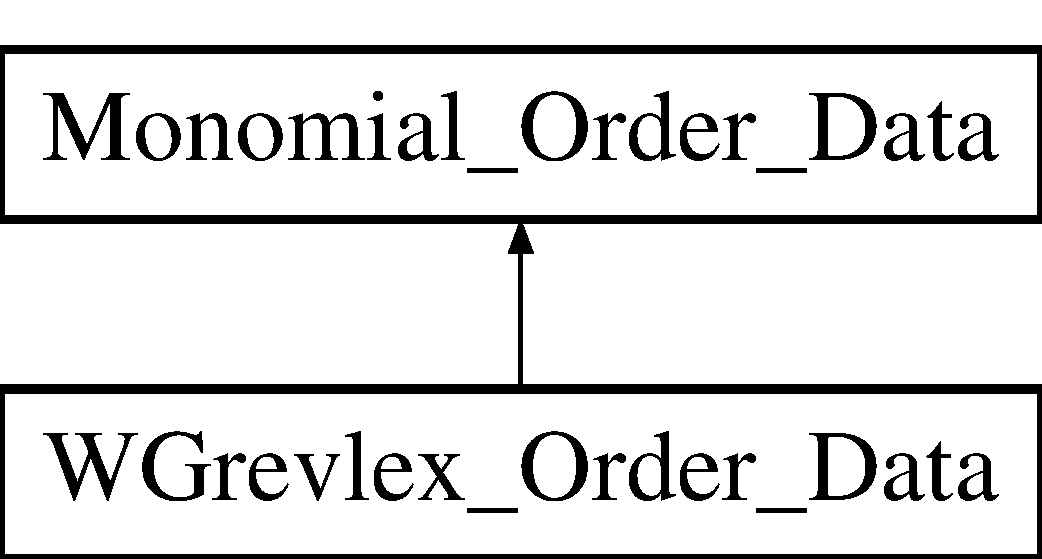
\includegraphics[height=2.000000cm]{group__orderinggroup}
\end{center}
\end{figure}
\index{Weighted\+\_\+\+Ordering@{Weighted\+\_\+\+Ordering}}\label{class_weighted___ordering}
\Hypertarget{group__orderinggroup_class_weighted___ordering}
\subsubsection{class Weighted\+\_\+\+Ordering}
interface to a weighted monomial ordering 

\begin{DoxyAuthor}{Author}
John Perry 
\end{DoxyAuthor}
\begin{DoxyDate}{Date}
2016 
\end{DoxyDate}
\begin{DoxySeeAlso}{See also}
\hyperlink{group__orderinggroup_class_monomial___ordering}{Monomial\+\_\+\+Ordering}
\end{DoxySeeAlso}
This class adds all of one method to \hyperlink{group__orderinggroup_class_monomial___ordering}{Monomial\+\_\+\+Ordering}. 

Definition at line 177 of file monomial\+\_\+ordering.\+hpp.

Inheritance diagram for Weighted\+\_\+\+Ordering\+:\begin{figure}[H]
\begin{center}
\leavevmode
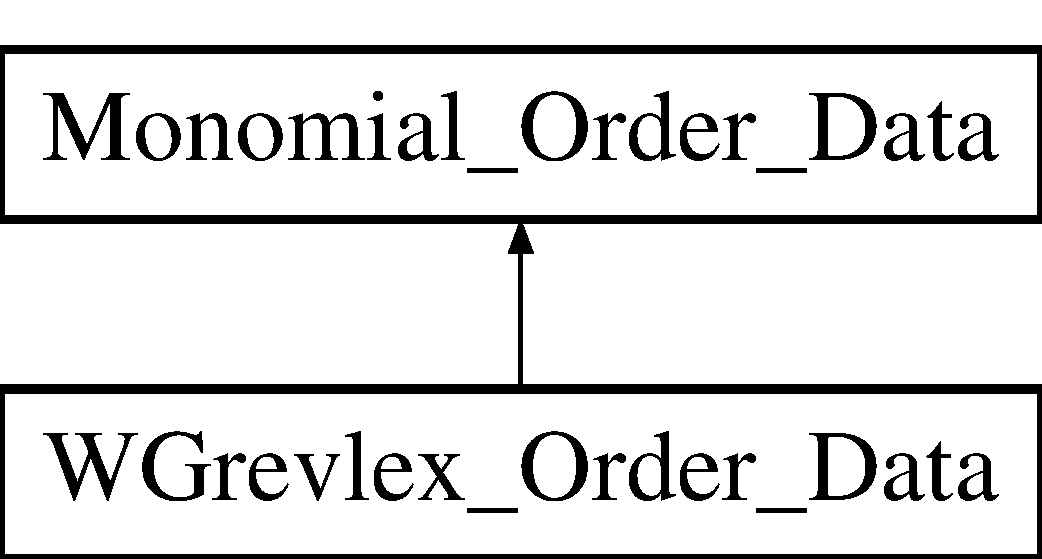
\includegraphics[height=3.000000cm]{group__orderinggroup}
\end{center}
\end{figure}
\subsubsection*{Public Member Functions}
\begin{Indent}\textbf{ Basic properties}\par
\begin{DoxyCompactItemize}
\item 
\mbox{\Hypertarget{group__orderinggroup_a5916f1631d5c30fe39dedcef96a3944e}\label{group__orderinggroup_a5916f1631d5c30fe39dedcef96a3944e}} 
virtual const W\+T\+\_\+\+T\+Y\+PE $\ast$ \hyperlink{group__orderinggroup_a5916f1631d5c30fe39dedcef96a3944e}{order\+\_\+weights} () const =0
\begin{DoxyCompactList}\small\item\em returns the weights used by this orderings \end{DoxyCompactList}\item 
\mbox{\Hypertarget{group__orderinggroup_a7f13d8c571e36bc29d2de39ace88bdd8}\label{group__orderinggroup_a7f13d8c571e36bc29d2de39ace88bdd8}} 
virtual N\+V\+A\+R\+\_\+\+T\+Y\+PE \hyperlink{group__orderinggroup_a7f13d8c571e36bc29d2de39ace88bdd8}{number\+\_\+of\+\_\+weights} () const =0
\begin{DoxyCompactList}\small\item\em returns the number of weights (same as number of indeterminates) \end{DoxyCompactList}\end{DoxyCompactItemize}
\end{Indent}
\index{W\+Grevlex@{W\+Grevlex}}\label{class_w_grevlex}
\Hypertarget{group__orderinggroup_class_w_grevlex}
\subsubsection{class W\+Grevlex}
the grevlex ordering for a specified number of variables 

\begin{DoxyAuthor}{Author}
John Perry 
\end{DoxyAuthor}
\begin{DoxyDate}{Date}
2016
\end{DoxyDate}
The grevlex ordering first compares the sums of the exponents, then the sums of all but the last exponent, then the sums of all but the last two exponents, and so forth, until either the sums differ or it runs out of variables. 

Definition at line 229 of file particular\+\_\+orderings.\+hpp.

Inheritance diagram for W\+Grevlex\+:\begin{figure}[H]
\begin{center}
\leavevmode
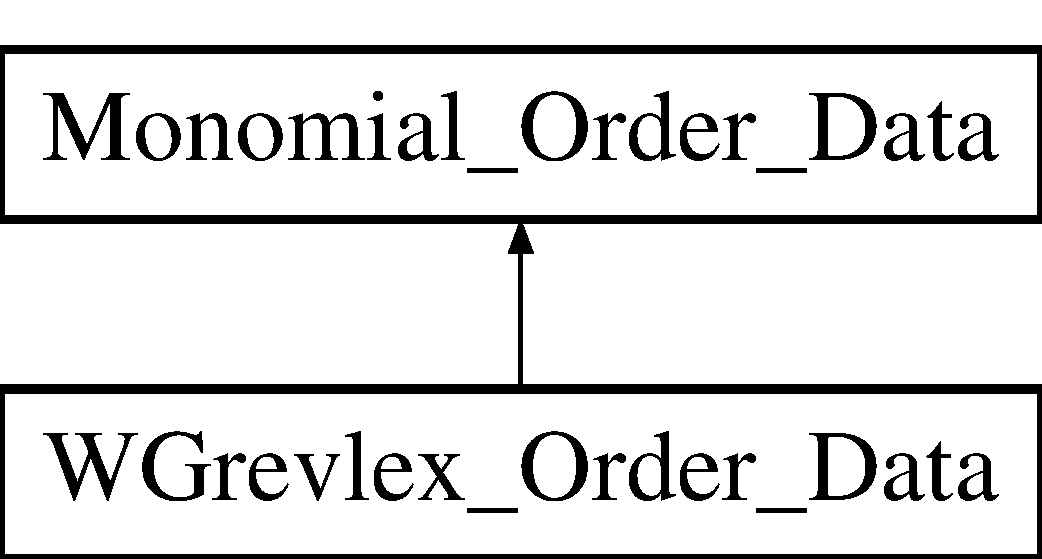
\includegraphics[height=3.000000cm]{group__orderinggroup}
\end{center}
\end{figure}
\subsubsection*{Public Member Functions}
\begin{Indent}\textbf{ Construction}\par
\begin{DoxyCompactItemize}
\item 
\mbox{\Hypertarget{group__orderinggroup_a0ac3e66fb20c098427f6a08c92fd3771}\label{group__orderinggroup_a0ac3e66fb20c098427f6a08c92fd3771}} 
\hyperlink{group__orderinggroup_a0ac3e66fb20c098427f6a08c92fd3771}{W\+Grevlex} (N\+V\+A\+R\+\_\+\+T\+Y\+PE, W\+T\+\_\+\+T\+Y\+PE $\ast$, bool=true)
\begin{DoxyCompactList}\small\item\em Creates a grevlex ordering specific to the specified number of variables, with the given weights. The final parameter indicates whether to apply the weights when breaking ties. \end{DoxyCompactList}\item 
\mbox{\Hypertarget{group__orderinggroup_a60f58ee49c04e416085a096c4e5798c1}\label{group__orderinggroup_a60f58ee49c04e416085a096c4e5798c1}} 
\hyperlink{group__orderinggroup_a60f58ee49c04e416085a096c4e5798c1}{W\+Grevlex} (\hyperlink{group___c_l_s_solvers_class_l_p___solvers_1_1_ray}{Ray} r, bool=true)
\begin{DoxyCompactList}\small\item\em Creates a weighted grevlex ordering using the specified ray. The final parameter indicates whether to apply the weights when breaking ties. \end{DoxyCompactList}\end{DoxyCompactItemize}
\end{Indent}
\begin{Indent}\textbf{ Basic properties}\par
\begin{DoxyCompactItemize}
\item 
\mbox{\Hypertarget{group__orderinggroup_a2eb6db0248ec4b205d15b5b1b2261db6}\label{group__orderinggroup_a2eb6db0248ec4b205d15b5b1b2261db6}} 
virtual const W\+T\+\_\+\+T\+Y\+PE $\ast$ \hyperlink{group__orderinggroup_a2eb6db0248ec4b205d15b5b1b2261db6}{order\+\_\+weights} () const override
\begin{DoxyCompactList}\small\item\em this weighted ordering's weights \end{DoxyCompactList}\item 
\mbox{\Hypertarget{group__orderinggroup_afd715e453ad062b40578438b1bbe10e9}\label{group__orderinggroup_afd715e453ad062b40578438b1bbe10e9}} 
virtual N\+V\+A\+R\+\_\+\+T\+Y\+PE \hyperlink{group__orderinggroup_afd715e453ad062b40578438b1bbe10e9}{number\+\_\+of\+\_\+weights} () const override
\begin{DoxyCompactList}\small\item\em returns the number of weights (same as number of indeterminates) \end{DoxyCompactList}\end{DoxyCompactItemize}
\end{Indent}
\begin{Indent}\textbf{ Comparison}\par
\begin{DoxyCompactItemize}
\item 
\mbox{\Hypertarget{group__orderinggroup_a547c267540f69917cadbeba621642f2a}\label{group__orderinggroup_a547c267540f69917cadbeba621642f2a}} 
virtual bool \hyperlink{group__orderinggroup_a547c267540f69917cadbeba621642f2a}{first\+\_\+larger} (const \hyperlink{group__polygroup_class_monomial}{Monomial} \&t, const \hyperlink{group__polygroup_class_monomial}{Monomial} \&u) const override
\begin{DoxyCompactList}\small\item\em returns {\ttfamily true} iff $t>u$ by weighted sums of successively fewer exponents \end{DoxyCompactList}\item 
\mbox{\Hypertarget{group__orderinggroup_a0e4327be4c18de7180ba2cd8c2f9d549}\label{group__orderinggroup_a0e4327be4c18de7180ba2cd8c2f9d549}} 
virtual bool \hyperlink{group__orderinggroup_a0e4327be4c18de7180ba2cd8c2f9d549}{first\+\_\+smaller} (const \hyperlink{group__polygroup_class_monomial}{Monomial} \&t, const \hyperlink{group__polygroup_class_monomial}{Monomial} \&u) const override
\begin{DoxyCompactList}\small\item\em returns {\ttfamily true} iff $t< u$ by weighted sums of successively fewer exponents \end{DoxyCompactList}\item 
\mbox{\Hypertarget{group__orderinggroup_a89e34bbf5098cc47d86468fcc334b670}\label{group__orderinggroup_a89e34bbf5098cc47d86468fcc334b670}} 
virtual bool \hyperlink{group__orderinggroup_a89e34bbf5098cc47d86468fcc334b670}{first\+\_\+larger\+\_\+than\+\_\+multiple} (const \hyperlink{group__polygroup_class_monomial}{Monomial} \&t, const \hyperlink{group__polygroup_class_monomial}{Monomial} \&u, const \hyperlink{group__polygroup_class_monomial}{Monomial} \&v) const override
\begin{DoxyCompactList}\small\item\em returns {\ttfamily true} iff $t>uv$ by weighted sums of successively fewer exponents \end{DoxyCompactList}\item 
D\+E\+G\+\_\+\+T\+Y\+PE \hyperlink{group__orderinggroup_ad7e630709c14774bac365c46b9455bab}{partial\+\_\+degree} (const \hyperlink{group__polygroup_class_monomial}{Monomial} \&t, N\+V\+A\+R\+\_\+\+T\+Y\+PE i) const
\item 
virtual int \hyperlink{group__orderinggroup_a0a65b26c9057d7f9d8c29ca3896cfd74}{cmp} (const \hyperlink{group__polygroup_class_monomial}{Monomial} \&t, const \hyperlink{group__polygroup_class_monomial}{Monomial} \&u) const override
\end{DoxyCompactItemize}
\end{Indent}
\begin{Indent}\textbf{ Utility}\par
\begin{DoxyCompactItemize}
\item 
\mbox{\Hypertarget{group__orderinggroup_a760db9641eb6993748fb26c211bd4bb0}\label{group__orderinggroup_a760db9641eb6993748fb26c211bd4bb0}} 
D\+E\+G\+\_\+\+T\+Y\+PE \hyperlink{group__orderinggroup_a760db9641eb6993748fb26c211bd4bb0}{compute\+\_\+ith\+\_\+weight} (const \hyperlink{group__polygroup_class_monomial}{Monomial} \&t, N\+V\+A\+R\+\_\+\+T\+Y\+PE i) const
\begin{DoxyCompactList}\small\item\em computes the weighted sum of the first i exponents \end{DoxyCompactList}\item 
\mbox{\Hypertarget{group__orderinggroup_a18ba60cd0a76da002303a11d362142d9}\label{group__orderinggroup_a18ba60cd0a76da002303a11d362142d9}} 
virtual void \hyperlink{group__orderinggroup_a18ba60cd0a76da002303a11d362142d9}{set\+\_\+data} (\hyperlink{group__polygroup_class_monomial}{Monomial} \&t) const override
\begin{DoxyCompactList}\small\item\em sets the \hyperlink{group__polygroup_class_monomial}{Monomial}'s {\ttfamily monomial\+\_\+ordering\+\_\+data} \end{DoxyCompactList}\end{DoxyCompactItemize}
\end{Indent}
\subsubsection*{Protected Attributes}
\begin{DoxyCompactItemize}
\item 
\mbox{\Hypertarget{group__orderinggroup_ac8355eb8a2145189fba8dcec4b47a22f}\label{group__orderinggroup_ac8355eb8a2145189fba8dcec4b47a22f}} 
const N\+V\+A\+R\+\_\+\+T\+Y\+PE \hyperlink{group__orderinggroup_ac8355eb8a2145189fba8dcec4b47a22f}{n}
\begin{DoxyCompactList}\small\item\em the number of variables, which should remain constant \end{DoxyCompactList}\item 
\mbox{\Hypertarget{group__orderinggroup_a73b55333b66eae11ee2e781c166b2421}\label{group__orderinggroup_a73b55333b66eae11ee2e781c166b2421}} 
bool \hyperlink{group__orderinggroup_a73b55333b66eae11ee2e781c166b2421}{thorough\+\_\+weighting}
\begin{DoxyCompactList}\small\item\em whether to apply the weights to all the variables \end{DoxyCompactList}\item 
\mbox{\Hypertarget{group__orderinggroup_a8a8d248da57c37bff15fe9400b1e04ff}\label{group__orderinggroup_a8a8d248da57c37bff15fe9400b1e04ff}} 
W\+T\+\_\+\+T\+Y\+PE $\ast$ \hyperlink{group__orderinggroup_a8a8d248da57c37bff15fe9400b1e04ff}{weights}
\begin{DoxyCompactList}\small\item\em the weights for this ordering \end{DoxyCompactList}\end{DoxyCompactItemize}
\subsubsection*{Friends}
\begin{Indent}\textbf{ I/O}\par
\begin{DoxyCompactItemize}
\item 
\mbox{\Hypertarget{group__orderinggroup_ad3b0454837c3ced9ffcd168bda55484b}\label{group__orderinggroup_ad3b0454837c3ced9ffcd168bda55484b}} 
ostream \& {\bfseries operator$<$$<$} (ostream \&os, const \hyperlink{group__orderinggroup_class_w_grevlex}{W\+Grevlex} \&word)
\end{DoxyCompactItemize}
\end{Indent}


\paragraph{Member Function Documentation}
\mbox{\Hypertarget{group__orderinggroup_a0a65b26c9057d7f9d8c29ca3896cfd74}\label{group__orderinggroup_a0a65b26c9057d7f9d8c29ca3896cfd74}} 
\index{W\+Grevlex@{W\+Grevlex}!cmp@{cmp}}
\index{cmp@{cmp}!W\+Grevlex@{W\+Grevlex}}
\subparagraph{\texorpdfstring{cmp()}{cmp()}}
{\footnotesize\ttfamily virtual int W\+Grevlex\+::cmp (\begin{DoxyParamCaption}\item[{const \hyperlink{group__polygroup_class_monomial}{Monomial} \&}]{t,  }\item[{const \hyperlink{group__polygroup_class_monomial}{Monomial} \&}]{u }\end{DoxyParamCaption}) const\hspace{0.3cm}{\ttfamily [inline]}, {\ttfamily [override]}, {\ttfamily [virtual]}}


\begin{DoxyParams}{Parameters}
{\em t} & a \hyperlink{group__polygroup_class_monomial}{Monomial}, to compare to $ u $ \\
\hline
{\em u} & a \hyperlink{group__polygroup_class_monomial}{Monomial}, to compare to $ t $ \\
\hline
\end{DoxyParams}
\begin{DoxyReturn}{Returns}
1 if $ t > u $ , -\/1 if $ t < u $ , and 0 otherwise 
\end{DoxyReturn}


Implements \hyperlink{group__orderinggroup_a9bc3155fc98b4d40c26118fa2114b827}{Monomial\+\_\+\+Ordering}.



Definition at line 284 of file particular\+\_\+orderings.\+hpp.

\mbox{\Hypertarget{group__orderinggroup_ad7e630709c14774bac365c46b9455bab}\label{group__orderinggroup_ad7e630709c14774bac365c46b9455bab}} 
\index{W\+Grevlex@{W\+Grevlex}!partial\+\_\+degree@{partial\+\_\+degree}}
\index{partial\+\_\+degree@{partial\+\_\+degree}!W\+Grevlex@{W\+Grevlex}}
\subparagraph{\texorpdfstring{partial\+\_\+degree()}{partial\_degree()}}
{\footnotesize\ttfamily D\+E\+G\+\_\+\+T\+Y\+PE W\+Grevlex\+::partial\+\_\+degree (\begin{DoxyParamCaption}\item[{const \hyperlink{group__polygroup_class_monomial}{Monomial} \&}]{t,  }\item[{N\+V\+A\+R\+\_\+\+T\+Y\+PE}]{i }\end{DoxyParamCaption}) const}

\begin{DoxyReturn}{Returns}
the weighted sum of the first i exponents 
\end{DoxyReturn}
\begin{DoxyWarning}{Warning}
Be sure that {\ttfamily t} has the correct ordering! 
\end{DoxyWarning}

\begin{DoxyParams}{Parameters}
{\em t} & a \hyperlink{group__polygroup_class_monomial}{Monomial} whose partial degree we want \\
\hline
{\em i} & index of the indeterminate to which we compute the degree \\
\hline
\end{DoxyParams}
\index{W\+Grevlex\+\_\+\+Order\+\_\+\+Data@{W\+Grevlex\+\_\+\+Order\+\_\+\+Data}}\label{class_w_grevlex___order___data}
\Hypertarget{group__orderinggroup_class_w_grevlex___order___data}
\subsubsection{class W\+Grevlex\+\_\+\+Order\+\_\+\+Data}
data for the weighted grevlex monomial ordering 

\begin{DoxyAuthor}{Author}
John Perry 
\end{DoxyAuthor}
\begin{DoxyDate}{Date}
2015
\end{DoxyDate}
The data involves an array of $n$ {\ttfamily D\+E\+G\+\_\+\+T\+Y\+PE}, where the first entry is a weighted sum of the first $n$ variables, the second entry is the {\itshape ordinary} sum of all but the last variable, etc. 

Definition at line 401 of file particular\+\_\+orderings.\+hpp.

Inheritance diagram for W\+Grevlex\+\_\+\+Order\+\_\+\+Data\+:\begin{figure}[H]
\begin{center}
\leavevmode
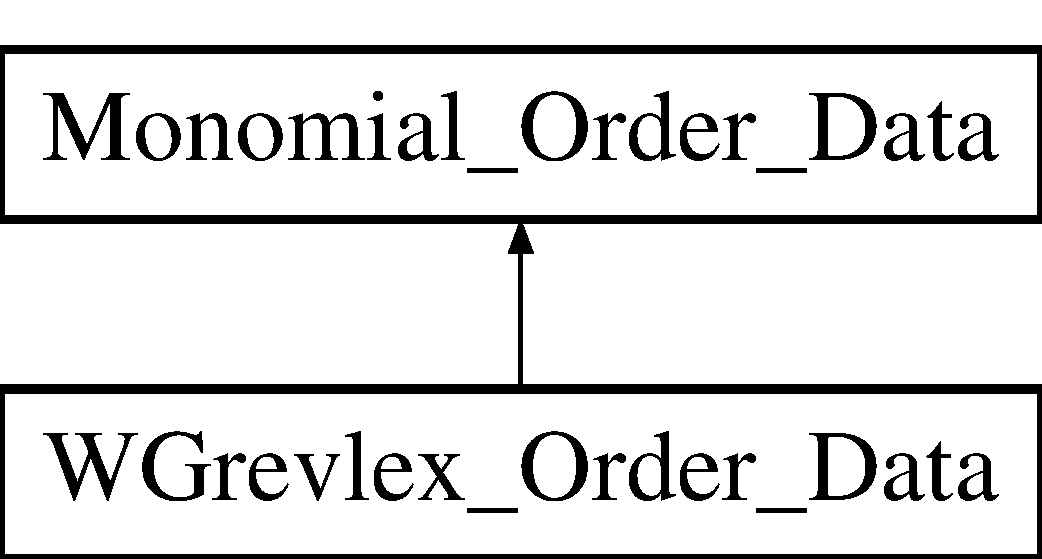
\includegraphics[height=2.000000cm]{group__orderinggroup}
\end{center}
\end{figure}
\subsubsection*{Public Member Functions}
\begin{Indent}\textbf{ Construction}\par
\begin{DoxyCompactItemize}
\item 
\hyperlink{group__orderinggroup_ad81bc55e04131b2d23371f6ce71d0422}{W\+Grevlex\+\_\+\+Order\+\_\+\+Data} (\hyperlink{group__polygroup_class_monomial}{Monomial} \&t)
\begin{DoxyCompactList}\small\item\em creates an array of partial weights of {\ttfamily t} \end{DoxyCompactList}\item 
\mbox{\Hypertarget{group__orderinggroup_a6074df104102f245666d996d100a859c}\label{group__orderinggroup_a6074df104102f245666d996d100a859c}} 
\hyperlink{group__orderinggroup_a6074df104102f245666d996d100a859c}{W\+Grevlex\+\_\+\+Order\+\_\+\+Data} (const \hyperlink{group__orderinggroup_class_w_grevlex___order___data}{W\+Grevlex\+\_\+\+Order\+\_\+\+Data} \&)
\begin{DoxyCompactList}\small\item\em copy constructor \end{DoxyCompactList}\item 
\mbox{\Hypertarget{group__orderinggroup_a84cb6a2eb475dc0bb4d7b2d7f21fa033}\label{group__orderinggroup_a84cb6a2eb475dc0bb4d7b2d7f21fa033}} 
virtual \hyperlink{group__orderinggroup_class_w_grevlex___order___data}{W\+Grevlex\+\_\+\+Order\+\_\+\+Data} $\ast$ \hyperlink{group__orderinggroup_a84cb6a2eb475dc0bb4d7b2d7f21fa033}{clone} () override
\begin{DoxyCompactList}\small\item\em clone constructor \end{DoxyCompactList}\end{DoxyCompactItemize}
\end{Indent}
\begin{Indent}\textbf{ Destruction}\par
\begin{DoxyCompactItemize}
\item 
\mbox{\Hypertarget{group__orderinggroup_aad8299f5ca80ad008cd62ba9e802abae}\label{group__orderinggroup_aad8299f5ca80ad008cd62ba9e802abae}} 
\hyperlink{group__orderinggroup_aad8299f5ca80ad008cd62ba9e802abae}{$\sim$\+W\+Grevlex\+\_\+\+Order\+\_\+\+Data} ()
\begin{DoxyCompactList}\small\item\em deletes the array of partial weights \end{DoxyCompactList}\end{DoxyCompactItemize}
\end{Indent}
\begin{Indent}\textbf{ returns the weighted sum of the first @f\$i@f\$ variables}\par
\begin{DoxyCompactItemize}
\item 
\mbox{\Hypertarget{group__orderinggroup_a91af5dd81fbb141ab08be35acbd001a1}\label{group__orderinggroup_a91af5dd81fbb141ab08be35acbd001a1}} 
D\+E\+G\+\_\+\+T\+Y\+PE {\bfseries operator\mbox{[}$\,$\mbox{]}} (N\+V\+A\+R\+\_\+\+T\+Y\+PE i) const
\item 
\mbox{\Hypertarget{group__orderinggroup_a8490fdd2ae55fa7a25f896003da8128a}\label{group__orderinggroup_a8490fdd2ae55fa7a25f896003da8128a}} 
virtual D\+E\+G\+\_\+\+T\+Y\+PE \hyperlink{group__orderinggroup_a8490fdd2ae55fa7a25f896003da8128a}{grading} (N\+V\+A\+R\+\_\+\+T\+Y\+PE i) const override
\begin{DoxyCompactList}\small\item\em default value is useless; orderings that supply gradings should redefine \end{DoxyCompactList}\end{DoxyCompactItemize}
\end{Indent}
\begin{Indent}\textbf{ Computation}\par
\begin{DoxyCompactItemize}
\item 
void \hyperlink{group__orderinggroup_a48f5464aaed30ba07d3eace69b2d87c1}{assign\+\_\+gradings} (\hyperlink{group__polygroup_class_monomial}{Monomial} \&t)
\begin{DoxyCompactList}\small\item\em assigns gradings to a pre-\/allocated array \end{DoxyCompactList}\end{DoxyCompactItemize}
\end{Indent}
\begin{Indent}\textbf{ Memory management}\par
\begin{DoxyCompactItemize}
\item 
\mbox{\Hypertarget{group__orderinggroup_ac81e3130c94b4f908e277c0c9a6f3d83}\label{group__orderinggroup_ac81e3130c94b4f908e277c0c9a6f3d83}} 
void $\ast$ \hyperlink{group__orderinggroup_ac81e3130c94b4f908e277c0c9a6f3d83}{operator new} (size\+\_\+t)
\begin{DoxyCompactList}\small\item\em requests memory form W\+Grevlex\+\_\+\+Ordering\textquotesingle{}s \hyperlink{group__memorygroup_class_grading___order___data___allocator}{Grading\+\_\+\+Order\+\_\+\+Data\+\_\+\+Allocator} \end{DoxyCompactList}\item 
\mbox{\Hypertarget{group__orderinggroup_aa512b345dc053fe960b5d955d73270c7}\label{group__orderinggroup_aa512b345dc053fe960b5d955d73270c7}} 
void \hyperlink{group__orderinggroup_aa512b345dc053fe960b5d955d73270c7}{operator delete} (void $\ast$)
\begin{DoxyCompactList}\small\item\em returns data to W\+Grevlex\+\_\+\+Ordering\textquotesingle{}s \hyperlink{group__memorygroup_class_grading___order___data___allocator}{Grading\+\_\+\+Order\+\_\+\+Data\+\_\+\+Allocator} \end{DoxyCompactList}\end{DoxyCompactItemize}
\end{Indent}
\subsubsection*{Protected Attributes}
\begin{DoxyCompactItemize}
\item 
\mbox{\Hypertarget{group__orderinggroup_a84079d31936d09b373b3cb3d79c5cec4}\label{group__orderinggroup_a84079d31936d09b373b3cb3d79c5cec4}} 
D\+E\+G\+\_\+\+T\+Y\+PE $\ast$ \hyperlink{group__orderinggroup_a84079d31936d09b373b3cb3d79c5cec4}{gradings}
\begin{DoxyCompactList}\small\item\em array of partial weighted sums of exponents \end{DoxyCompactList}\item 
\mbox{\Hypertarget{group__orderinggroup_a4ec320689813725e8f1e0b23334e6cbd}\label{group__orderinggroup_a4ec320689813725e8f1e0b23334e6cbd}} 
const N\+V\+A\+R\+\_\+\+T\+Y\+PE \hyperlink{group__orderinggroup_a4ec320689813725e8f1e0b23334e6cbd}{number\+\_\+of\+\_\+gradings}
\begin{DoxyCompactList}\small\item\em length of {\ttfamily gradings} \end{DoxyCompactList}\end{DoxyCompactItemize}


\paragraph{Constructor \& Destructor Documentation}
\mbox{\Hypertarget{group__orderinggroup_ad81bc55e04131b2d23371f6ce71d0422}\label{group__orderinggroup_ad81bc55e04131b2d23371f6ce71d0422}} 
\index{W\+Grevlex\+\_\+\+Order\+\_\+\+Data@{W\+Grevlex\+\_\+\+Order\+\_\+\+Data}!W\+Grevlex\+\_\+\+Order\+\_\+\+Data@{W\+Grevlex\+\_\+\+Order\+\_\+\+Data}}
\index{W\+Grevlex\+\_\+\+Order\+\_\+\+Data@{W\+Grevlex\+\_\+\+Order\+\_\+\+Data}!W\+Grevlex\+\_\+\+Order\+\_\+\+Data@{W\+Grevlex\+\_\+\+Order\+\_\+\+Data}}
\subparagraph{\texorpdfstring{W\+Grevlex\+\_\+\+Order\+\_\+\+Data()}{WGrevlex\_Order\_Data()}}
{\footnotesize\ttfamily W\+Grevlex\+\_\+\+Order\+\_\+\+Data\+::\+W\+Grevlex\+\_\+\+Order\+\_\+\+Data (\begin{DoxyParamCaption}\item[{\hyperlink{group__polygroup_class_monomial}{Monomial} \&}]{t }\end{DoxyParamCaption})}



creates an array of partial weights of {\ttfamily t} 

\begin{DoxyWarning}{Warning}
Assign the correct ordering to {\ttfamily t} first! 
\end{DoxyWarning}

\begin{DoxyParams}{Parameters}
{\em t} & a \hyperlink{group__polygroup_class_monomial}{Monomial} whose weights {\ttfamily this} will cache \\
\hline
\end{DoxyParams}


Definition at line 405 of file particular\+\_\+orderings.\+cpp.



\paragraph{Member Function Documentation}
\mbox{\Hypertarget{group__orderinggroup_a48f5464aaed30ba07d3eace69b2d87c1}\label{group__orderinggroup_a48f5464aaed30ba07d3eace69b2d87c1}} 
\index{W\+Grevlex\+\_\+\+Order\+\_\+\+Data@{W\+Grevlex\+\_\+\+Order\+\_\+\+Data}!assign\+\_\+gradings@{assign\+\_\+gradings}}
\index{assign\+\_\+gradings@{assign\+\_\+gradings}!W\+Grevlex\+\_\+\+Order\+\_\+\+Data@{W\+Grevlex\+\_\+\+Order\+\_\+\+Data}}
\subparagraph{\texorpdfstring{assign\+\_\+gradings()}{assign\_gradings()}}
{\footnotesize\ttfamily void W\+Grevlex\+\_\+\+Order\+\_\+\+Data\+::assign\+\_\+gradings (\begin{DoxyParamCaption}\item[{\hyperlink{group__polygroup_class_monomial}{Monomial} \&}]{t }\end{DoxyParamCaption})}



assigns gradings to a pre-\/allocated array 

\begin{DoxyWarning}{Warning}
This does not create the array if it does not exist already! 
\end{DoxyWarning}

\begin{DoxyParams}{Parameters}
{\em t} & a \hyperlink{group__polygroup_class_monomial}{Monomial} whose gradings we want \\
\hline
\end{DoxyParams}


Definition at line 391 of file particular\+\_\+orderings.\+cpp.



\subsection{Function Documentation}
\mbox{\Hypertarget{group__orderinggroup_ga22e2d4b10cd30468c9e67351ab78aa27}\label{group__orderinggroup_ga22e2d4b10cd30468c9e67351ab78aa27}} 
\index{Monomial Orderings@{Monomial Orderings}!nonsingular@{nonsingular}}
\index{nonsingular@{nonsingular}!Monomial Orderings@{Monomial Orderings}}
\subsubsection{\texorpdfstring{nonsingular()}{nonsingular()}}
{\footnotesize\ttfamily bool nonsingular (\begin{DoxyParamCaption}\item[{N\+V\+A\+R\+\_\+\+T\+Y\+PE}]{m,  }\item[{N\+V\+A\+R\+\_\+\+T\+Y\+PE}]{n,  }\item[{const W\+T\+\_\+\+T\+Y\+PE $\ast$$\ast$}]{A }\end{DoxyParamCaption})}



verifies that a matrix supplied for an ordering is not nonsingular 

\begin{DoxyAuthor}{Author}
John Perry 
\end{DoxyAuthor}
\begin{DoxyDate}{Date}
2016
\end{DoxyDate}
For the time being, this reduces the matrix to upper triangular form (if possible) and then checks that the diagonal is nonzero. 
\begin{DoxyParams}{Parameters}
{\em m} & number of rows in the matrix referenced by {\ttfamily A} \\
\hline
{\em n} & number of columns in the matrix referenced by {\ttfamily A} \\
\hline
{\em A} & array of at least $ m\times n $ elements \\
\hline
\end{DoxyParams}
\begin{DoxyReturn}{Returns}
{\ttfamily true} if and only if the matrix referenced by {\ttfamily A} is nonsingular 
\end{DoxyReturn}


Definition at line 566 of file particular\+\_\+orderings.\+cpp.


\hypertarget{group__polygroup}{}\section{Polynomials}
\label{group__polygroup}\index{Polynomials@{Polynomials}}


classes related to the structure of polynomials  


\subsection*{Classes}
\begin{DoxyCompactItemize}
\item 
class \hyperlink{group__polygroup_class_abstract___polynomial}{Abstract\+\_\+\+Polynomial}
\begin{DoxyCompactList}\small\item\em The general class of a polynomial.  \hyperlink{group__polygroup_class_abstract___polynomial}{More...}\end{DoxyCompactList}\item 
class \hyperlink{group__polygroup_class_constant___polynomial}{Constant\+\_\+\+Polynomial}
\begin{DoxyCompactList}\small\item\em A \hyperlink{group__polygroup_class_constant___polynomial}{Constant\+\_\+\+Polynomial} is a polynomial that should not change.  \hyperlink{group__polygroup_class_constant___polynomial}{More...}\end{DoxyCompactList}\item 
class \hyperlink{group__polygroup_class_dense___univariate___integer___polynomial}{Dense\+\_\+\+Univariate\+\_\+\+Integer\+\_\+\+Polynomial}
\begin{DoxyCompactList}\small\item\em quick-\/'n-\/dirty Dense\+\_\+\+Univariate integer polynomial class  \hyperlink{group__polygroup_class_dense___univariate___integer___polynomial}{More...}\end{DoxyCompactList}\item 
class \hyperlink{group__polygroup_class_dense___univariate___rational___polynomial}{Dense\+\_\+\+Univariate\+\_\+\+Rational\+\_\+\+Polynomial}
\begin{DoxyCompactList}\small\item\em quick-\/'n-\/dirty Dense\+\_\+\+Univariate rational polynomial class  \hyperlink{group__polygroup_class_dense___univariate___rational___polynomial}{More...}\end{DoxyCompactList}\item 
class \hyperlink{group__polygroup_class_double___buffered___polynomial}{Double\+\_\+\+Buffered\+\_\+\+Polynomial}
\begin{DoxyCompactList}\small\item\em Polynomials implemented using double buffers.

A double-\/buffered polynomial maintains at all times two arrays to store its terms. (Technically, it retains four arrays\+: two for the monomials, and two for the coefficients.) Any operation that might change the {\itshape length} of the polynomials reads the data in one buffer and writes the result to the other buffer. The goal of this approach is to avoid the penalties associated with allocating, deallocating, and traversing the nodes of a linked list.  \hyperlink{group__polygroup_class_double___buffered___polynomial}{More...}\end{DoxyCompactList}\item 
class \hyperlink{group__polygroup_class_indeterminate}{Indeterminate}
\begin{DoxyCompactList}\small\item\em Implementation of indeterminates, for easier building of polynomials.  \hyperlink{group__polygroup_class_indeterminate}{More...}\end{DoxyCompactList}\item 
class \hyperlink{group__polygroup_class_monomial}{Monomial}
\begin{DoxyCompactList}\small\item\em Implementation of monomials.  \hyperlink{group__polygroup_class_monomial}{More...}\end{DoxyCompactList}\item 
class \hyperlink{group__polygroup_class_monomial___ideal}{Monomial\+\_\+\+Ideal}
\begin{DoxyCompactList}\small\item\em A class for monomial ideals.  \hyperlink{group__polygroup_class_monomial___ideal}{More...}\end{DoxyCompactList}\item 
class \hyperlink{group__polygroup_class_monomial___ideal___variables___exception}{Monomial\+\_\+\+Ideal\+\_\+\+Variables\+\_\+\+Exception}
\begin{DoxyCompactList}\small\item\em exceptions for \hyperlink{group__polygroup_class_monomial}{Monomial} Ideals  \hyperlink{group__polygroup_class_monomial___ideal___variables___exception}{More...}\end{DoxyCompactList}\item 
class \hyperlink{group__polygroup_class_monomial___node}{Monomial\+\_\+\+Node}
\begin{DoxyCompactList}\small\item\em Tool for \hyperlink{group__polygroup_class_polynomial___linked___list}{Polynomial\+\_\+\+Linked\+\_\+\+List}.  \hyperlink{group__polygroup_class_monomial___node}{More...}\end{DoxyCompactList}\item 
class \hyperlink{group__polygroup_class_mutable___polynomial}{Mutable\+\_\+\+Polynomial}
\begin{DoxyCompactList}\small\item\em Polynomials that need arithmetic typically descend from this class.  \hyperlink{group__polygroup_class_mutable___polynomial}{More...}\end{DoxyCompactList}\item 
class \hyperlink{group__polygroup_class_polynomial___geobucket}{Polynomial\+\_\+\+Geobucket}
\begin{DoxyCompactList}\small\item\em Implementation of geobuckets.  \hyperlink{group__polygroup_class_polynomial___geobucket}{More...}\end{DoxyCompactList}\item 
class \hyperlink{group__polygroup_class_polynomial___linked___list}{Polynomial\+\_\+\+Linked\+\_\+\+List}
\begin{DoxyCompactList}\small\item\em Polynomials represented as a doubly linked list.  \hyperlink{group__polygroup_class_polynomial___linked___list}{More...}\end{DoxyCompactList}\item 
class \hyperlink{group__polygroup_class_polynomial___ring}{Polynomial\+\_\+\+Ring}
\begin{DoxyCompactList}\small\item\em Encapsulates information about a polynomial ring for easy access\+: ground field, number of indeterminates, {$\dots$}.  \hyperlink{group__polygroup_class_polynomial___ring}{More...}\end{DoxyCompactList}\end{DoxyCompactItemize}
\subsection*{Functions}
\begin{DoxyCompactItemize}
\item 
list$<$ \hyperlink{group__polygroup_class_monomial}{Monomial} $>$ \hyperlink{group__polygroup_gaf4655e829836ead5fe2ce766fb0cebbc}{colon\+\_\+ideal\+\_\+without\+\_\+ideals} (const list$<$ \hyperlink{group__polygroup_class_monomial}{Monomial} $>$ \&U, const \hyperlink{group__polygroup_class_monomial}{Monomial} \&t)
\begin{DoxyCompactList}\small\item\em Computes the generators of an ideal and a new generator, given the ideal\textquotesingle{}s generators. No monomial ideal machinery required. \end{DoxyCompactList}\item 
list$<$ \hyperlink{group__polygroup_class_abstract___polynomial}{Abstract\+\_\+\+Polynomial} $\ast$ $>$ \hyperlink{group__polygroup_gaa458dfbf51ecbb98f93bf8f0133725d0}{cyclic\+\_\+n} (N\+V\+A\+R\+\_\+\+T\+Y\+PE n, \hyperlink{group___fields_group_class_prime___field}{Prime\+\_\+\+Field} \&F, bool homog, \hyperlink{group__orderinggroup_class_monomial___ordering}{Monomial\+\_\+\+Ordering} $\ast$mord=generic\+\_\+grevlex\+\_\+ptr)
\begin{DoxyCompactList}\small\item\em generates the Cyclic-\/ $ n $ system \end{DoxyCompactList}\end{DoxyCompactItemize}


\subsection{Detailed Description}
classes related to the structure of polynomials 



\subsection{Class Documentation}
\index{Abstract\+\_\+\+Polynomial@{Abstract\+\_\+\+Polynomial}}\label{class_abstract___polynomial}
\Hypertarget{group__polygroup_class_abstract___polynomial}
\subsubsection{class Abstract\+\_\+\+Polynomial}
The general class of a polynomial. 

\begin{DoxyAuthor}{Author}
John Perry 
\end{DoxyAuthor}
\begin{DoxyDate}{Date}
2015
\end{DoxyDate}
This class encapsulates the minimum feature set necessary for our application. Naturally, it must be possible to identify a leading monomial and coefficient. Every polynomial must also be able to produce an iterator; indicate its its length (number of monomials), and its number of variables; describe its ground field; and produce a zero polynomial of the same type (this has its uses).

\begin{DoxyWarning}{Warning}
Monomials should have the same number of variables, and coefficients should all come from the same field. Behavior is undefined if these assumptions are violated. From an algebraic point of view, it doesn't make much sense to violate them, anyway; (in/pro)ject into a different ring if you want to screw around like this. 
\end{DoxyWarning}
\begin{Desc}
\item[Examples\+: ]\par
\hyperlink{test_cyclicn_8cpp-example}{test\+\_\+cyclicn.\+cpp}, \hyperlink{test_dynamic_8cpp-example}{test\+\_\+dynamic.\+cpp}, \hyperlink{test_f4_8cpp-example}{test\+\_\+f4.\+cpp}, \hyperlink{test_f4_dynamic_8cpp-example}{test\+\_\+f4\+\_\+dynamic.\+cpp}, and \hyperlink{user_interface_8cpp-example}{user\+\_\+interface.\+cpp}.\end{Desc}


Definition at line 101 of file polynomial.\+hpp.

Inheritance diagram for Abstract\+\_\+\+Polynomial\+:\begin{figure}[H]
\begin{center}
\leavevmode
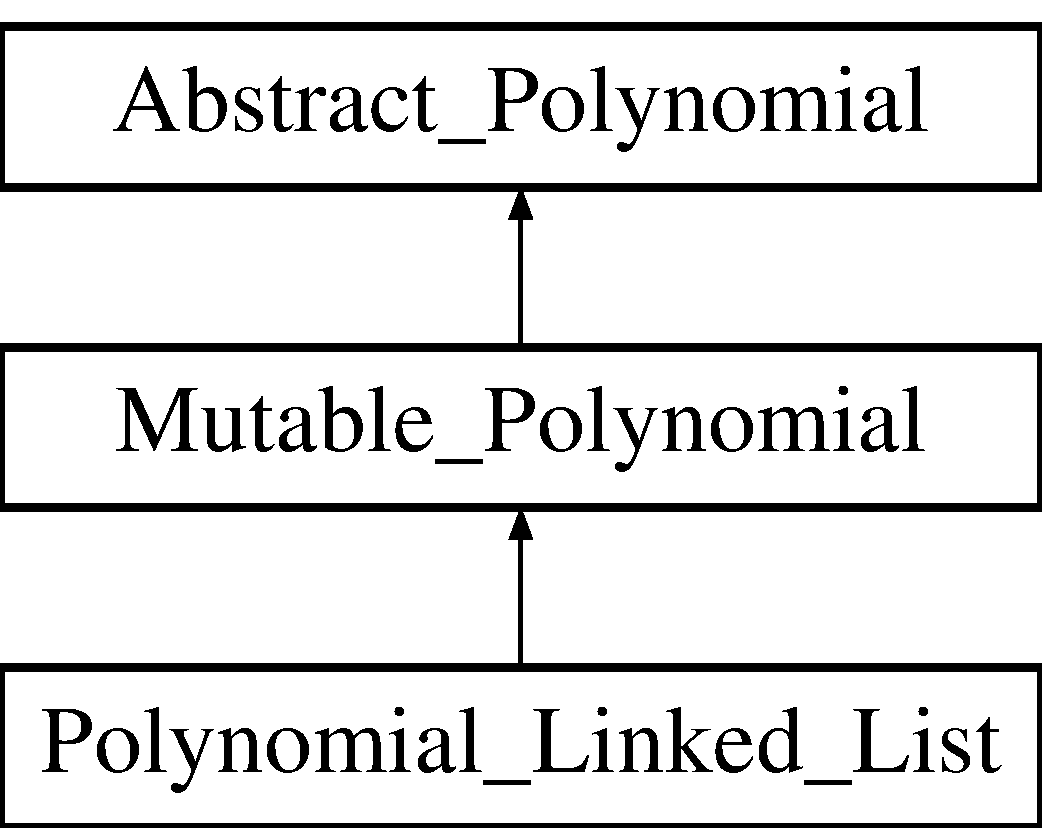
\includegraphics[height=3.000000cm]{group__polygroup}
\end{center}
\end{figure}
\subsubsection*{Public Member Functions}
\begin{Indent}\textbf{ Construction}\par
\begin{DoxyCompactItemize}
\item 
\hyperlink{group__polygroup_af72cda5555005f99c9844fece4e5ca46}{Abstract\+\_\+\+Polynomial} (\hyperlink{group__polygroup_class_polynomial___ring}{Polynomial\+\_\+\+Ring} \&ring, const \hyperlink{group__orderinggroup_class_monomial___ordering}{Monomial\+\_\+\+Ordering} $\ast$ordering)
\end{DoxyCompactItemize}
\end{Indent}
\begin{Indent}\textbf{ Destruction}\par
\begin{DoxyCompactItemize}
\item 
\mbox{\Hypertarget{group__polygroup_a5082a214ab62d3d5aad6d294926be8e2}\label{group__polygroup_a5082a214ab62d3d5aad6d294926be8e2}} 
virtual \hyperlink{group__polygroup_a5082a214ab62d3d5aad6d294926be8e2}{$\sim$\+Abstract\+\_\+\+Polynomial} ()
\begin{DoxyCompactList}\small\item\em deletes the strategy, if there is one \end{DoxyCompactList}\end{DoxyCompactItemize}
\end{Indent}
\begin{Indent}\textbf{ Basic properties}\par
\begin{DoxyCompactItemize}
\item 
\mbox{\Hypertarget{group__polygroup_abf1f531c0004bf37874e98eee42dc0f4}\label{group__polygroup_abf1f531c0004bf37874e98eee42dc0f4}} 
\hyperlink{group__polygroup_class_polynomial___ring}{Polynomial\+\_\+\+Ring} \& \hyperlink{group__polygroup_abf1f531c0004bf37874e98eee42dc0f4}{base\+\_\+ring} () const
\begin{DoxyCompactList}\small\item\em ring in which this polynomial resides \end{DoxyCompactList}\item 
\mbox{\Hypertarget{group__polygroup_a9569282b79afba5d6393a75844437702}\label{group__polygroup_a9569282b79afba5d6393a75844437702}} 
const \hyperlink{group___fields_group_class_prime___field}{Prime\+\_\+\+Field} \& \hyperlink{group__polygroup_a9569282b79afba5d6393a75844437702}{ground\+\_\+field} () const
\begin{DoxyCompactList}\small\item\em ground field -- all coefficients should be in this field \end{DoxyCompactList}\item 
\mbox{\Hypertarget{group__polygroup_a4419bbe47e14683f2903c47bee8e04af}\label{group__polygroup_a4419bbe47e14683f2903c47bee8e04af}} 
unsigned \hyperlink{group__polygroup_a4419bbe47e14683f2903c47bee8e04af}{number\+\_\+of\+\_\+variables} () const
\begin{DoxyCompactList}\small\item\em number of variables -- all monomials should agree with this (though it is never tested by the class) \end{DoxyCompactList}\item 
\mbox{\Hypertarget{group__polygroup_a36a3b3b5132246f9e916b91d8d5a1c76}\label{group__polygroup_a36a3b3b5132246f9e916b91d8d5a1c76}} 
const \hyperlink{group__orderinggroup_class_monomial___ordering}{Monomial\+\_\+\+Ordering} $\ast$ \hyperlink{group__polygroup_a36a3b3b5132246f9e916b91d8d5a1c76}{monomial\+\_\+ordering} () const
\begin{DoxyCompactList}\small\item\em reports leading monomial's monomial ordering \end{DoxyCompactList}\item 
\mbox{\Hypertarget{group__polygroup_a9186ed0f55c5cc4ecb1b9bc11ba9f679}\label{group__polygroup_a9186ed0f55c5cc4ecb1b9bc11ba9f679}} 
virtual \hyperlink{group__polygroup_class_monomial}{Monomial} \& \hyperlink{group__polygroup_a9186ed0f55c5cc4ecb1b9bc11ba9f679}{leading\+\_\+monomial} () const =0
\begin{DoxyCompactList}\small\item\em leading monomial -- call after \hyperlink{group__polygroup_a1fcdd29c324c660ea935197c39e682f2}{sort\+\_\+by\+\_\+order()}! \end{DoxyCompactList}\item 
\mbox{\Hypertarget{group__polygroup_a511ce8e997fe3fd1141293d256e25fad}\label{group__polygroup_a511ce8e997fe3fd1141293d256e25fad}} 
virtual \hyperlink{group___fields_group_class_prime___field___element}{Prime\+\_\+\+Field\+\_\+\+Element} \hyperlink{group__polygroup_a511ce8e997fe3fd1141293d256e25fad}{leading\+\_\+coefficient} () const =0
\begin{DoxyCompactList}\small\item\em leading coefficient -- call after \hyperlink{group__polygroup_a1fcdd29c324c660ea935197c39e682f2}{sort\+\_\+by\+\_\+order()}! \end{DoxyCompactList}\item 
\mbox{\Hypertarget{group__polygroup_a48f4c3c030ca66a9386cd71f71d5def7}\label{group__polygroup_a48f4c3c030ca66a9386cd71f71d5def7}} 
virtual unsigned \hyperlink{group__polygroup_a48f4c3c030ca66a9386cd71f71d5def7}{length} () const =0
\begin{DoxyCompactList}\small\item\em number of monomials \end{DoxyCompactList}\item 
\mbox{\Hypertarget{group__polygroup_afb4895702dd56895a792850a831c2f51}\label{group__polygroup_afb4895702dd56895a792850a831c2f51}} 
virtual bool \hyperlink{group__polygroup_afb4895702dd56895a792850a831c2f51}{is\+\_\+zero} () const =0
\begin{DoxyCompactList}\small\item\em is this polynomial zero? \end{DoxyCompactList}\item 
\mbox{\Hypertarget{group__polygroup_af43d43a17c02c38c3ba3e71710e226bf}\label{group__polygroup_af43d43a17c02c38c3ba3e71710e226bf}} 
virtual bool \hyperlink{group__polygroup_af43d43a17c02c38c3ba3e71710e226bf}{can\+\_\+reduce} (\hyperlink{group__polygroup_class_abstract___polynomial}{Abstract\+\_\+\+Polynomial} \&other) const
\begin{DoxyCompactList}\small\item\em can {\ttfamily this} reduce {\ttfamily other}? \end{DoxyCompactList}\item 
\mbox{\Hypertarget{group__polygroup_a3b7b27fc293408d0d34d60dc6a090c79}\label{group__polygroup_a3b7b27fc293408d0d34d60dc6a090c79}} 
virtual \hyperlink{group__strategygroup_class_poly___strategy___data}{Poly\+\_\+\+Strategy\+\_\+\+Data} $\ast$ \hyperlink{group__polygroup_a3b7b27fc293408d0d34d60dc6a090c79}{strategy} () const
\begin{DoxyCompactList}\small\item\em strategy related information \end{DoxyCompactList}\item 
\mbox{\Hypertarget{group__polygroup_aa619f56a2df5d0077335709ac11de039}\label{group__polygroup_aa619f56a2df5d0077335709ac11de039}} 
virtual D\+E\+G\+\_\+\+T\+Y\+PE \hyperlink{group__polygroup_aa619f56a2df5d0077335709ac11de039}{standard\+\_\+degree} () const
\begin{DoxyCompactList}\small\item\em maximum sum of exponents for any monomial \end{DoxyCompactList}\item 
virtual D\+E\+G\+\_\+\+T\+Y\+PE \hyperlink{group__polygroup_a231aa84c74183943142952d8035b1943}{weighted\+\_\+degree} (const W\+T\+\_\+\+T\+Y\+PE $\ast$w=nullptr) const
\end{DoxyCompactItemize}
\end{Indent}
\begin{Indent}\textbf{ Computation}\par
\begin{DoxyCompactItemize}
\item 
\mbox{\Hypertarget{group__polygroup_ab50acaac5654329c0299d5694a25b1ed}\label{group__polygroup_ab50acaac5654329c0299d5694a25b1ed}} 
virtual \hyperlink{group__polygroup_class_abstract___polynomial}{Abstract\+\_\+\+Polynomial} $\ast$ \hyperlink{group__polygroup_ab50acaac5654329c0299d5694a25b1ed}{zero\+\_\+polynomial} () const =0
\begin{DoxyCompactList}\small\item\em new zero polynomial of this same type \end{DoxyCompactList}\item 
\mbox{\Hypertarget{group__polygroup_aacee94ef63116201c91c7d65779097d8}\label{group__polygroup_aacee94ef63116201c91c7d65779097d8}} 
virtual \hyperlink{group__polygroup_class_abstract___polynomial}{Abstract\+\_\+\+Polynomial} $\ast$ \hyperlink{group__polygroup_aacee94ef63116201c91c7d65779097d8}{monomial\+\_\+multiple} (const \hyperlink{group__polygroup_class_monomial}{Monomial} \&) const =0
\begin{DoxyCompactList}\small\item\em multiple of this and $u$ \end{DoxyCompactList}\item 
\mbox{\Hypertarget{group__polygroup_a53b0ed425ff4bbbf01818005d6003d59}\label{group__polygroup_a53b0ed425ff4bbbf01818005d6003d59}} 
virtual \hyperlink{group__polygroup_class_abstract___polynomial}{Abstract\+\_\+\+Polynomial} $\ast$ \hyperlink{group__polygroup_a53b0ed425ff4bbbf01818005d6003d59}{scalar\+\_\+multiple} (const \hyperlink{group___fields_group_class_prime___field___element}{Prime\+\_\+\+Field\+\_\+\+Element} \&) const =0
\begin{DoxyCompactList}\small\item\em multiple of this and $c$ \end{DoxyCompactList}\item 
\mbox{\Hypertarget{group__polygroup_a780b8c4b18ae1df16ce680f79d9ace7b}\label{group__polygroup_a780b8c4b18ae1df16ce680f79d9ace7b}} 
void \hyperlink{group__polygroup_a780b8c4b18ae1df16ce680f79d9ace7b}{set\+\_\+strategy} (\hyperlink{group__strategygroup_class_poly___strategy___data}{Poly\+\_\+\+Strategy\+\_\+\+Data} $\ast$psd)
\begin{DoxyCompactList}\small\item\em sets the polynomial's strategy to {\ttfamily psd} \end{DoxyCompactList}\end{DoxyCompactItemize}
\end{Indent}
\begin{Indent}\textbf{ Ordering monomials}\par
\begin{DoxyCompactItemize}
\item 
virtual void \hyperlink{group__polygroup_a12e023570eb675343c4b7ed635a031dc}{set\+\_\+monomial\+\_\+ordering} (const \hyperlink{group__orderinggroup_class_monomial___ordering}{Monomial\+\_\+\+Ordering} $\ast$order, bool sort\+\_\+anew=true)=0
\begin{DoxyCompactList}\small\item\em set the monomial ordering and sort the polynomials (optionally, but by default) \end{DoxyCompactList}\item 
virtual void \hyperlink{group__polygroup_a1fcdd29c324c660ea935197c39e682f2}{sort\+\_\+by\+\_\+order} ()=0
\begin{DoxyCompactList}\small\item\em sort according to the leading monomial's ordering \end{DoxyCompactList}\end{DoxyCompactItemize}
\end{Indent}
\begin{Indent}\textbf{ Iteration}\par
\begin{DoxyCompactItemize}
\item 
\mbox{\Hypertarget{group__polygroup_a9cb8460694b7fceaa5a22ae58c73ebe7}\label{group__polygroup_a9cb8460694b7fceaa5a22ae58c73ebe7}} 
virtual \hyperlink{group___iterator_group_class_polynomial___iterator}{Polynomial\+\_\+\+Iterator} $\ast$ \hyperlink{group__polygroup_a9cb8460694b7fceaa5a22ae58c73ebe7}{new\+\_\+iterator} () const =0
\begin{DoxyCompactList}\small\item\em An iterator that poses no risk of modifying the polynomial. \end{DoxyCompactList}\item 
\mbox{\Hypertarget{group__polygroup_ad8da27c2d5e41d6e81d15d756eebf868}\label{group__polygroup_ad8da27c2d5e41d6e81d15d756eebf868}} 
virtual \hyperlink{group___iterator_group_class_polynomial___iterator}{Polynomial\+\_\+\+Iterator} $\ast$ \hyperlink{group__polygroup_ad8da27c2d5e41d6e81d15d756eebf868}{begin} () const =0
\begin{DoxyCompactList}\small\item\em returns an iterator to the polynomial's leading monomial \end{DoxyCompactList}\item 
\mbox{\Hypertarget{group__polygroup_aa769b074a39e5eac6526101d77e2e53f}\label{group__polygroup_aa769b074a39e5eac6526101d77e2e53f}} 
virtual \hyperlink{group___iterator_group_class_polynomial___iterator}{Polynomial\+\_\+\+Iterator} $\ast$ \hyperlink{group__polygroup_aa769b074a39e5eac6526101d77e2e53f}{end} () const =0
\begin{DoxyCompactList}\small\item\em iterator to last monomial \end{DoxyCompactList}\end{DoxyCompactItemize}
\end{Indent}
\subsubsection*{Protected Attributes}
\begin{DoxyCompactItemize}
\item 
\mbox{\Hypertarget{group__polygroup_a551ade20b7dcd96c227dd0401f6ffbbe}\label{group__polygroup_a551ade20b7dcd96c227dd0401f6ffbbe}} 
\hyperlink{group__polygroup_class_polynomial___ring}{Polynomial\+\_\+\+Ring} \& \hyperlink{group__polygroup_a551ade20b7dcd96c227dd0401f6ffbbe}{R}
\begin{DoxyCompactList}\small\item\em data about polynomial ring \end{DoxyCompactList}\item 
\mbox{\Hypertarget{group__polygroup_a764336acff942ed6d6e160b5d62f90c1}\label{group__polygroup_a764336acff942ed6d6e160b5d62f90c1}} 
\hyperlink{group__strategygroup_class_poly___strategy___data}{Poly\+\_\+\+Strategy\+\_\+\+Data} $\ast$ \hyperlink{group__polygroup_a764336acff942ed6d6e160b5d62f90c1}{strat} = nullptr
\begin{DoxyCompactList}\small\item\em data for computational strategies \end{DoxyCompactList}\end{DoxyCompactItemize}
\subsubsection*{I/O}
\begin{DoxyCompactItemize}
\item 
\mbox{\Hypertarget{group__polygroup_adbbb6af1fb79d5794af42e28d584641b}\label{group__polygroup_adbbb6af1fb79d5794af42e28d584641b}} 
virtual void \hyperlink{group__polygroup_adbbb6af1fb79d5794af42e28d584641b}{print} (ostream \&os=cout) const
\begin{DoxyCompactList}\small\item\em prints the polynomial to {\ttfamily os} \end{DoxyCompactList}\item 
\mbox{\Hypertarget{group__polygroup_a597dc990980f1936e86dbf8940dbeecd}\label{group__polygroup_a597dc990980f1936e86dbf8940dbeecd}} 
virtual void \hyperlink{group__polygroup_a597dc990980f1936e86dbf8940dbeecd}{println} (ostream \&os=cout) const
\begin{DoxyCompactList}\small\item\em prints the polynomial to {\ttfamily os}, followed by a carriage return \end{DoxyCompactList}\item 
\mbox{\Hypertarget{group__polygroup_a69dfd6bd725e126d2476826fb345c5f6}\label{group__polygroup_a69dfd6bd725e126d2476826fb345c5f6}} 
virtual void \hyperlink{group__polygroup_a69dfd6bd725e126d2476826fb345c5f6}{printlncout} () const
\begin{DoxyCompactList}\small\item\em prints the polynomial to {\ttfamily cout}, followed by a carriage return \end{DoxyCompactList}\item 
\mbox{\Hypertarget{group__polygroup_aadc14212f0cbdb81df9977916cc13798}\label{group__polygroup_aadc14212f0cbdb81df9977916cc13798}} 
ostream \& \hyperlink{group__polygroup_aadc14212f0cbdb81df9977916cc13798}{operator$<$$<$} (ostream \&os, const \hyperlink{group__polygroup_class_abstract___polynomial}{Abstract\+\_\+\+Polynomial} \&p)
\begin{DoxyCompactList}\small\item\em output \end{DoxyCompactList}\end{DoxyCompactItemize}


\paragraph{Constructor \& Destructor Documentation}
\mbox{\Hypertarget{group__polygroup_af72cda5555005f99c9844fece4e5ca46}\label{group__polygroup_af72cda5555005f99c9844fece4e5ca46}} 
\index{Abstract\+\_\+\+Polynomial@{Abstract\+\_\+\+Polynomial}!Abstract\+\_\+\+Polynomial@{Abstract\+\_\+\+Polynomial}}
\index{Abstract\+\_\+\+Polynomial@{Abstract\+\_\+\+Polynomial}!Abstract\+\_\+\+Polynomial@{Abstract\+\_\+\+Polynomial}}
\subparagraph{\texorpdfstring{Abstract\+\_\+\+Polynomial()}{Abstract\_Polynomial()}}
{\footnotesize\ttfamily Abstract\+\_\+\+Polynomial\+::\+Abstract\+\_\+\+Polynomial (\begin{DoxyParamCaption}\item[{\hyperlink{group__polygroup_class_polynomial___ring}{Polynomial\+\_\+\+Ring} \&}]{ring,  }\item[{const \hyperlink{group__orderinggroup_class_monomial___ordering}{Monomial\+\_\+\+Ordering} $\ast$}]{ordering }\end{DoxyParamCaption})\hspace{0.3cm}{\ttfamily [inline]}}


\begin{DoxyParams}{Parameters}
{\em ring} & the polynomial ring in which this polynomial will reside \\
\hline
{\em ordering} & the monomial ordering that first sorts the monomials \\
\hline
\end{DoxyParams}


Definition at line 110 of file polynomial.\+hpp.



\paragraph{Member Function Documentation}
\mbox{\Hypertarget{group__polygroup_a12e023570eb675343c4b7ed635a031dc}\label{group__polygroup_a12e023570eb675343c4b7ed635a031dc}} 
\index{Abstract\+\_\+\+Polynomial@{Abstract\+\_\+\+Polynomial}!set\+\_\+monomial\+\_\+ordering@{set\+\_\+monomial\+\_\+ordering}}
\index{set\+\_\+monomial\+\_\+ordering@{set\+\_\+monomial\+\_\+ordering}!Abstract\+\_\+\+Polynomial@{Abstract\+\_\+\+Polynomial}}
\subparagraph{\texorpdfstring{set\+\_\+monomial\+\_\+ordering()}{set\_monomial\_ordering()}}
{\footnotesize\ttfamily virtual void Abstract\+\_\+\+Polynomial\+::set\+\_\+monomial\+\_\+ordering (\begin{DoxyParamCaption}\item[{const \hyperlink{group__orderinggroup_class_monomial___ordering}{Monomial\+\_\+\+Ordering} $\ast$}]{order,  }\item[{bool}]{sort\+\_\+anew = {\ttfamily true} }\end{DoxyParamCaption})\hspace{0.3cm}{\ttfamily [pure virtual]}}



set the monomial ordering and sort the polynomials (optionally, but by default) 


\begin{DoxyParams}{Parameters}
{\em order} & new monomial ordering \\
\hline
{\em sort\+\_\+anew} & whether to sort the polynomial anew \\
\hline
\end{DoxyParams}
\begin{DoxyWarning}{Warning}
In most cases you will want to sort anew {\itshape immediately} after setting the ordering. Otherwise, the monomials may be in the wrong order! That is therefore the default behavior of this function, but in case you don't want to sort, that option is provided. 
\end{DoxyWarning}


Implemented in \hyperlink{group__polygroup_af9b1dee3a8ca9fb26a6e069ea70ea5df}{Polynomial\+\_\+\+Linked\+\_\+\+List}, \hyperlink{group__polygroup_a539835f92490fbbb5ba3b37e4f80ef49}{Constant\+\_\+\+Polynomial}, \hyperlink{group__polygroup_ad3298b3201f53d0ddaa657206c140ca8}{Polynomial\+\_\+\+Geobucket}, and \hyperlink{group__polygroup_aa81be797dcced4e663d3fe54f6501ed6}{Double\+\_\+\+Buffered\+\_\+\+Polynomial}.

\mbox{\Hypertarget{group__polygroup_a1fcdd29c324c660ea935197c39e682f2}\label{group__polygroup_a1fcdd29c324c660ea935197c39e682f2}} 
\index{Abstract\+\_\+\+Polynomial@{Abstract\+\_\+\+Polynomial}!sort\+\_\+by\+\_\+order@{sort\+\_\+by\+\_\+order}}
\index{sort\+\_\+by\+\_\+order@{sort\+\_\+by\+\_\+order}!Abstract\+\_\+\+Polynomial@{Abstract\+\_\+\+Polynomial}}
\subparagraph{\texorpdfstring{sort\+\_\+by\+\_\+order()}{sort\_by\_order()}}
{\footnotesize\ttfamily virtual void Abstract\+\_\+\+Polynomial\+::sort\+\_\+by\+\_\+order (\begin{DoxyParamCaption}{ }\end{DoxyParamCaption})\hspace{0.3cm}{\ttfamily [pure virtual]}}



sort according to the leading monomial's ordering 

Note that it makes sense to sort even \hyperlink{group__polygroup_class_constant___polynomial}{Constant\+\_\+\+Polynomial}'s, as it is not the polynomial that changes, only the order of its monomials. 

Implemented in \hyperlink{group__polygroup_a254bec60707b34bd26ef9d9bb08a4fe9}{Polynomial\+\_\+\+Linked\+\_\+\+List}, \hyperlink{group__polygroup_a808018b52eca472a7a1b2995e403f35a}{Constant\+\_\+\+Polynomial}, \hyperlink{group__polygroup_a41e751eee1614e26ebba39a9f81f7993}{Double\+\_\+\+Buffered\+\_\+\+Polynomial}, and \hyperlink{group__polygroup_ad3c705cb5c03be2ed62fea65101d1195}{Polynomial\+\_\+\+Geobucket}.

\begin{Desc}
\item[Examples\+: ]\par
\hyperlink{user_interface_8cpp-example}{user\+\_\+interface.\+cpp}.\end{Desc}
\mbox{\Hypertarget{group__polygroup_a231aa84c74183943142952d8035b1943}\label{group__polygroup_a231aa84c74183943142952d8035b1943}} 
\index{Abstract\+\_\+\+Polynomial@{Abstract\+\_\+\+Polynomial}!weighted\+\_\+degree@{weighted\+\_\+degree}}
\index{weighted\+\_\+degree@{weighted\+\_\+degree}!Abstract\+\_\+\+Polynomial@{Abstract\+\_\+\+Polynomial}}
\subparagraph{\texorpdfstring{weighted\+\_\+degree()}{weighted\_degree()}}
{\footnotesize\ttfamily D\+E\+G\+\_\+\+T\+Y\+PE Abstract\+\_\+\+Polynomial\+::weighted\+\_\+degree (\begin{DoxyParamCaption}\item[{const W\+T\+\_\+\+T\+Y\+PE $\ast$}]{w = {\ttfamily nullptr} }\end{DoxyParamCaption}) const\hspace{0.3cm}{\ttfamily [virtual]}}

\begin{DoxyReturn}{Returns}
largest weighted sum of exponents for any monomial 
\end{DoxyReturn}

\begin{DoxyParams}{Parameters}
{\em w} & weights to use for weighted degree\\
\hline
\end{DoxyParams}
Equivalent to \hyperlink{group__polygroup_aa619f56a2df5d0077335709ac11de039}{standard\+\_\+degree()} if {\ttfamily w == nullptr}. 

Definition at line 110 of file polynomial.\+cpp.

\index{Constant\+\_\+\+Polynomial@{Constant\+\_\+\+Polynomial}}\label{class_constant___polynomial}
\Hypertarget{group__polygroup_class_constant___polynomial}
\subsubsection{class Constant\+\_\+\+Polynomial}
A \hyperlink{group__polygroup_class_constant___polynomial}{Constant\+\_\+\+Polynomial} is a polynomial that should not change. 

\begin{DoxyAuthor}{Author}
John Perry 
\end{DoxyAuthor}
\begin{DoxyDate}{Date}
2015
\end{DoxyDate}
We do allow on change at this level\+: to resort the monomials. We do not consider this a real change (it's still the same polynomial), and in any case even this is effectively unimplemented right now (unless you set up the polynomial with unsorted terms, in which case sorting them helps). \begin{Desc}
\item[Examples\+: ]\par
\hyperlink{test_4by4_8cpp-example}{test\+\_\+4by4.\+cpp}, \hyperlink{test_cab_es1_8cpp-example}{test\+\_\+cab\+\_\+es1.\+cpp}, \hyperlink{test_cab_es2_8cpp-example}{test\+\_\+cab\+\_\+es2.\+cpp}, \hyperlink{test_cab_es4_8cpp-example}{test\+\_\+cab\+\_\+es4.\+cpp}, \hyperlink{test_cab_es5_8cpp-example}{test\+\_\+cab\+\_\+es5.\+cpp}, \hyperlink{test_cab_es6_8cpp-example}{test\+\_\+cab\+\_\+es6.\+cpp}, \hyperlink{test_cab_es9_8cpp-example}{test\+\_\+cab\+\_\+es9.\+cpp}, \hyperlink{test_cyclic4_8cpp-example}{test\+\_\+cyclic4.\+cpp}, \hyperlink{test_cyclicn_8cpp-example}{test\+\_\+cyclicn.\+cpp}, \hyperlink{test_dynamic_8cpp-example}{test\+\_\+dynamic.\+cpp}, \hyperlink{test_f4_8cpp-example}{test\+\_\+f4.\+cpp}, \hyperlink{test_f4_dynamic_8cpp-example}{test\+\_\+f4\+\_\+dynamic.\+cpp}, and \hyperlink{user_interface_8cpp-example}{user\+\_\+interface.\+cpp}.\end{Desc}


Definition at line 89 of file polynomial\+\_\+array.\+hpp.

Inheritance diagram for Constant\+\_\+\+Polynomial\+:\begin{figure}[H]
\begin{center}
\leavevmode
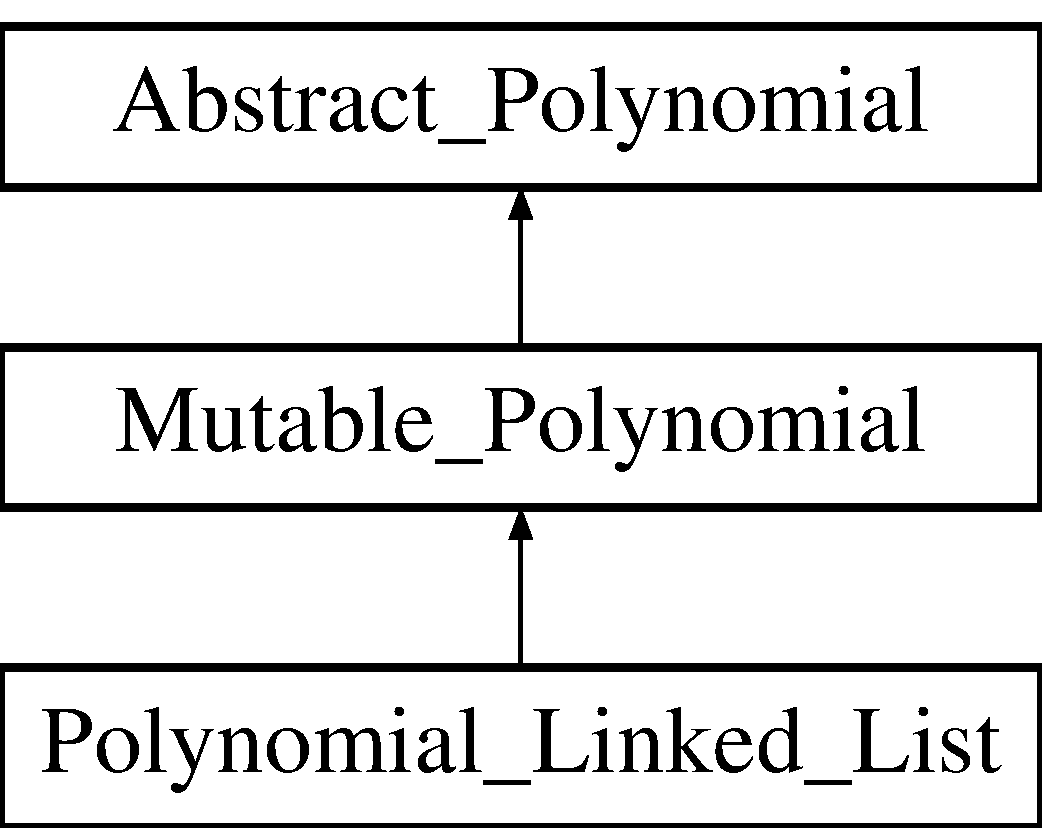
\includegraphics[height=2.000000cm]{group__polygroup}
\end{center}
\end{figure}
\subsubsection*{Public Member Functions}
\begin{Indent}\textbf{ Construction}\par
\begin{DoxyCompactItemize}
\item 
\hyperlink{group__polygroup_a17e78adc39df3472a0610b17c906898f}{Constant\+\_\+\+Polynomial} (unsigned \hyperlink{group__polygroup_a9a6bcfaf1f4d6260b39f6abfb2b646ea}{length}, \hyperlink{group__polygroup_class_polynomial___ring}{Polynomial\+\_\+\+Ring} \&\hyperlink{group__polygroup_a551ade20b7dcd96c227dd0401f6ffbbe}{R}, const \hyperlink{group__polygroup_class_monomial}{Monomial} $\ast$mons, const \hyperlink{group___fields_group_class_prime___field___element}{Prime\+\_\+\+Field\+\_\+\+Element} $\ast$coeffs, const \hyperlink{group__orderinggroup_class_monomial___ordering}{Monomial\+\_\+\+Ordering} $\ast$order=nullptr)
\item 
\hyperlink{group__polygroup_aa64fa434a206b1b29f27b09d36060dac}{Constant\+\_\+\+Polynomial} (unsigned \hyperlink{group__polygroup_a9a6bcfaf1f4d6260b39f6abfb2b646ea}{length}, \hyperlink{group__polygroup_class_polynomial___ring}{Polynomial\+\_\+\+Ring} \&\hyperlink{group__polygroup_a551ade20b7dcd96c227dd0401f6ffbbe}{R}, const vector$<$ \hyperlink{group__polygroup_class_monomial}{Monomial} $\ast$$>$ mons, const C\+O\+E\+F\+\_\+\+T\+Y\+PE $\ast$coeffs, unsigned start)
\item 
\hyperlink{group__polygroup_ac8bd342911678053e14cf72af46819c5}{Constant\+\_\+\+Polynomial} (\hyperlink{group__polygroup_class_polynomial___ring}{Polynomial\+\_\+\+Ring} \&\hyperlink{group__polygroup_a551ade20b7dcd96c227dd0401f6ffbbe}{R}, const list$<$ \hyperlink{group__polygroup_class_monomial}{Monomial} $>$ \&mons, const list$<$ \hyperlink{group___fields_group_class_prime___field___element}{Prime\+\_\+\+Field\+\_\+\+Element} $>$ \&coeffs, const \hyperlink{group__orderinggroup_class_monomial___ordering}{Monomial\+\_\+\+Ordering} $\ast$order=nullptr)
\item 
\hyperlink{group__polygroup_abbc487b48dbf5d0dc25dfb419a341ea5}{Constant\+\_\+\+Polynomial} (unsigned \hyperlink{group__polygroup_a9a6bcfaf1f4d6260b39f6abfb2b646ea}{length}, \hyperlink{group__polygroup_class_polynomial___ring}{Polynomial\+\_\+\+Ring} \&\hyperlink{group__polygroup_a551ade20b7dcd96c227dd0401f6ffbbe}{R}, const \hyperlink{group__orderinggroup_class_monomial___ordering}{Monomial\+\_\+\+Ordering} $\ast$order=generic\+\_\+grevlex\+\_\+ptr)
\item 
\mbox{\Hypertarget{group__polygroup_a3e0e3066356e56c7245bb517b4e04284}\label{group__polygroup_a3e0e3066356e56c7245bb517b4e04284}} 
\hyperlink{group__polygroup_a3e0e3066356e56c7245bb517b4e04284}{Constant\+\_\+\+Polynomial} (const \hyperlink{group__polygroup_class_abstract___polynomial}{Abstract\+\_\+\+Polynomial} \&p)
\begin{DoxyCompactList}\small\item\em Creates a constant polynomial copy of p. \end{DoxyCompactList}\item 
\mbox{\Hypertarget{group__polygroup_a9fd6527f6fe525668cc53e0d2aa384ca}\label{group__polygroup_a9fd6527f6fe525668cc53e0d2aa384ca}} 
\hyperlink{group__polygroup_a9fd6527f6fe525668cc53e0d2aa384ca}{Constant\+\_\+\+Polynomial} (\hyperlink{group__polygroup_class_polynomial___ring}{Polynomial\+\_\+\+Ring} \&, const \hyperlink{group__orderinggroup_class_monomial___ordering}{Monomial\+\_\+\+Ordering} $\ast$, uint64\+\_\+t, uint64\+\_\+t $\ast$)
\begin{DoxyCompactList}\small\item\em from serial data \end{DoxyCompactList}\end{DoxyCompactItemize}
\end{Indent}
\begin{Indent}\textbf{ Destruction}\par
\begin{DoxyCompactItemize}
\item 
\mbox{\Hypertarget{group__polygroup_aa535c175852c76c71e0ef556d8e25579}\label{group__polygroup_aa535c175852c76c71e0ef556d8e25579}} 
{\bfseries $\sim$\+Constant\+\_\+\+Polynomial} ()
\end{DoxyCompactItemize}
\end{Indent}
\begin{Indent}\textbf{ Basic properties}\par
\begin{DoxyCompactItemize}
\item 
virtual void \hyperlink{group__polygroup_a539835f92490fbbb5ba3b37e4f80ef49}{set\+\_\+monomial\+\_\+ordering} (const \hyperlink{group__orderinggroup_class_monomial___ordering}{Monomial\+\_\+\+Ordering} $\ast$order, bool sort\+\_\+anew=true) override
\begin{DoxyCompactList}\small\item\em sets the ordering of monomials in this polynomial \end{DoxyCompactList}\item 
virtual void \hyperlink{group__polygroup_a808018b52eca472a7a1b2995e403f35a}{sort\+\_\+by\+\_\+order} () override
\begin{DoxyCompactList}\small\item\em sort by order \end{DoxyCompactList}\item 
virtual \hyperlink{group__polygroup_class_monomial}{Monomial} \& \hyperlink{group__polygroup_a08a102d5d0f33bc9cc604316e6256788}{leading\+\_\+monomial} () const override
\item 
virtual \hyperlink{group___fields_group_class_prime___field___element}{Prime\+\_\+\+Field\+\_\+\+Element} \hyperlink{group__polygroup_ab1451de8d6d9f9b0c7df2aef7b32625d}{leading\+\_\+coefficient} () const override
\item 
virtual unsigned \hyperlink{group__polygroup_a9a6bcfaf1f4d6260b39f6abfb2b646ea}{length} () const override
\item 
virtual bool \hyperlink{group__polygroup_a14a9a2dbab454f5b20441a51a6000888}{is\+\_\+zero} () const override
\end{DoxyCompactItemize}
\end{Indent}
\begin{Indent}\textbf{ Computation}\par
\begin{DoxyCompactItemize}
\item 
virtual \hyperlink{group__polygroup_class_constant___polynomial}{Constant\+\_\+\+Polynomial} $\ast$ \hyperlink{group__polygroup_af7933d269e23525f1f357c0e00bc71ea}{zero\+\_\+polynomial} () const override
\item 
virtual \hyperlink{group__polygroup_class_constant___polynomial}{Constant\+\_\+\+Polynomial} $\ast$ \hyperlink{group__polygroup_ae0af1a1cf7c7eed390b25a951a685da2}{monomial\+\_\+multiple} (const \hyperlink{group__polygroup_class_monomial}{Monomial} \&t) const override
\item 
virtual \hyperlink{group__polygroup_class_constant___polynomial}{Constant\+\_\+\+Polynomial} $\ast$ \hyperlink{group__polygroup_afd8bdd523c36fbde64df0bf36a0f4e77}{scalar\+\_\+multiple} (const \hyperlink{group___fields_group_class_prime___field___element}{Prime\+\_\+\+Field\+\_\+\+Element} \&c) const override
\end{DoxyCompactItemize}
\end{Indent}
\begin{Indent}\textbf{ Iteration}\par
\begin{DoxyCompactItemize}
\item 
\mbox{\Hypertarget{group__polygroup_ab69dc9c6fcea390d0ab3c36379a3ee9c}\label{group__polygroup_ab69dc9c6fcea390d0ab3c36379a3ee9c}} 
virtual \hyperlink{group___iterator_group_class_constant___polynomial___iterator}{Constant\+\_\+\+Polynomial\+\_\+\+Iterator} $\ast$ \hyperlink{group__polygroup_ab69dc9c6fcea390d0ab3c36379a3ee9c}{new\+\_\+iterator} () const override
\begin{DoxyCompactList}\small\item\em an iterator that poses no risk of modifying the polynomial \end{DoxyCompactList}\item 
\mbox{\Hypertarget{group__polygroup_aaf17fe042545372d6ceb5858f3e3afac}\label{group__polygroup_aaf17fe042545372d6ceb5858f3e3afac}} 
virtual \hyperlink{group___iterator_group_class_polynomial___iterator}{Polynomial\+\_\+\+Iterator} $\ast$ \hyperlink{group__polygroup_aaf17fe042545372d6ceb5858f3e3afac}{begin} () const override
\begin{DoxyCompactList}\small\item\em iterator to the first element \end{DoxyCompactList}\item 
\mbox{\Hypertarget{group__polygroup_aee1e3c821a17fa655b02bab7d2bec2f2}\label{group__polygroup_aee1e3c821a17fa655b02bab7d2bec2f2}} 
virtual \hyperlink{group___iterator_group_class_polynomial___iterator}{Polynomial\+\_\+\+Iterator} $\ast$ \hyperlink{group__polygroup_aee1e3c821a17fa655b02bab7d2bec2f2}{end} () const override
\begin{DoxyCompactList}\small\item\em iterator to the last element \end{DoxyCompactList}\end{DoxyCompactItemize}
\end{Indent}
\begin{Indent}\textbf{ Serialization}\par
\begin{DoxyCompactItemize}
\item 
uint64\+\_\+t $\ast$ \hyperlink{group__polygroup_aafc581313f33e812add8db45cfaa1492}{serialized} (uint64\+\_\+t \&size)
\end{DoxyCompactItemize}
\end{Indent}
\subsubsection*{Protected Attributes}
\begin{DoxyCompactItemize}
\item 
\mbox{\Hypertarget{group__polygroup_a0b78eef8746e334e8db176d479e734b9}\label{group__polygroup_a0b78eef8746e334e8db176d479e734b9}} 
\hyperlink{group___fields_group_class_prime___field___element}{Prime\+\_\+\+Field\+\_\+\+Element} $\ast$ \hyperlink{group__polygroup_a0b78eef8746e334e8db176d479e734b9}{A}
\begin{DoxyCompactList}\small\item\em array of coefficients, in one-\/to-\/one correspondence with {\ttfamily M} \end{DoxyCompactList}\item 
\mbox{\Hypertarget{group__polygroup_ab82cd79a8965d04717a0c82ae79ff4b4}\label{group__polygroup_ab82cd79a8965d04717a0c82ae79ff4b4}} 
unsigned \hyperlink{group__polygroup_ab82cd79a8965d04717a0c82ae79ff4b4}{head}
\begin{DoxyCompactList}\small\item\em location of leading term in array (always farther left) \end{DoxyCompactList}\item 
\mbox{\Hypertarget{group__polygroup_aec23722090ac440cee1be3cb54ed5d16}\label{group__polygroup_aec23722090ac440cee1be3cb54ed5d16}} 
\hyperlink{group__polygroup_class_monomial}{Monomial} $\ast$ \hyperlink{group__polygroup_aec23722090ac440cee1be3cb54ed5d16}{M}
\begin{DoxyCompactList}\small\item\em array of monomials, in one-\/to-\/one correspondence with {\ttfamily A} \end{DoxyCompactList}\item 
\mbox{\Hypertarget{group__polygroup_acbd3e3d53eefdfae5b59431d40ccd11b}\label{group__polygroup_acbd3e3d53eefdfae5b59431d40ccd11b}} 
unsigned \hyperlink{group__polygroup_acbd3e3d53eefdfae5b59431d40ccd11b}{m}
\begin{DoxyCompactList}\small\item\em position {\bfseries after} last monomial \end{DoxyCompactList}\end{DoxyCompactItemize}
\subsubsection*{Friends}
\begin{DoxyCompactItemize}
\item 
\mbox{\Hypertarget{group__polygroup_ab740f854a3b6a761b4deaf1dc3fc4dbf}\label{group__polygroup_ab740f854a3b6a761b4deaf1dc3fc4dbf}} 
class \hyperlink{group__polygroup_ab740f854a3b6a761b4deaf1dc3fc4dbf}{Constant\+\_\+\+Polynomial\+\_\+\+Iterator}
\begin{DoxyCompactList}\small\item\em to iterate without changing {\ttfamily this} \end{DoxyCompactList}\item 
\mbox{\Hypertarget{group__polygroup_aefeb273b3b448966d0c8b5041a420d20}\label{group__polygroup_aefeb273b3b448966d0c8b5041a420d20}} 
class \hyperlink{group__polygroup_aefeb273b3b448966d0c8b5041a420d20}{Mutable\+\_\+\+Constant\+\_\+\+Polynomial\+\_\+\+Iterator}
\begin{DoxyCompactList}\small\item\em to iterate and possibly change {\ttfamily this} \end{DoxyCompactList}\end{DoxyCompactItemize}


\paragraph{Constructor \& Destructor Documentation}
\mbox{\Hypertarget{group__polygroup_a17e78adc39df3472a0610b17c906898f}\label{group__polygroup_a17e78adc39df3472a0610b17c906898f}} 
\index{Constant\+\_\+\+Polynomial@{Constant\+\_\+\+Polynomial}!Constant\+\_\+\+Polynomial@{Constant\+\_\+\+Polynomial}}
\index{Constant\+\_\+\+Polynomial@{Constant\+\_\+\+Polynomial}!Constant\+\_\+\+Polynomial@{Constant\+\_\+\+Polynomial}}
\subparagraph{\texorpdfstring{Constant\+\_\+\+Polynomial()}{Constant\_Polynomial()}\hspace{0.1cm}{\footnotesize\ttfamily [1/4]}}
{\footnotesize\ttfamily Constant\+\_\+\+Polynomial\+::\+Constant\+\_\+\+Polynomial (\begin{DoxyParamCaption}\item[{unsigned}]{length,  }\item[{\hyperlink{group__polygroup_class_polynomial___ring}{Polynomial\+\_\+\+Ring} \&}]{R,  }\item[{const \hyperlink{group__polygroup_class_monomial}{Monomial} $\ast$}]{mons,  }\item[{const \hyperlink{group___fields_group_class_prime___field___element}{Prime\+\_\+\+Field\+\_\+\+Element} $\ast$}]{coeffs,  }\item[{const \hyperlink{group__orderinggroup_class_monomial___ordering}{Monomial\+\_\+\+Ordering} $\ast$}]{order = {\ttfamily nullptr} }\end{DoxyParamCaption})}


\begin{DoxyParams}{Parameters}
{\em length} & how long {\ttfamily this} should be \\
\hline
{\em R} & parent ring \\
\hline
{\em mons} & array of \hyperlink{group__polygroup_class_monomial}{Monomial} to populate the terms \\
\hline
{\em coeffs} & array of coefficients to populate the terms, in same order as {\ttfamily mons} \\
\hline
{\em order} & monomial ordering used to first sort the polynomial; {\ttfamily nullptr} gives {\ttfamily generic\+\_\+grevlex\+\_\+ptr} \\
\hline
\end{DoxyParams}
We assume that mons and coeffs both have length n. We do not check that the monomials have the same number of variables, nor that the coefficients come from the same field, nor do we sort the monomials. The client needs to do this! 

Definition at line 54 of file polynomial\+\_\+array.\+cpp.

\mbox{\Hypertarget{group__polygroup_aa64fa434a206b1b29f27b09d36060dac}\label{group__polygroup_aa64fa434a206b1b29f27b09d36060dac}} 
\index{Constant\+\_\+\+Polynomial@{Constant\+\_\+\+Polynomial}!Constant\+\_\+\+Polynomial@{Constant\+\_\+\+Polynomial}}
\index{Constant\+\_\+\+Polynomial@{Constant\+\_\+\+Polynomial}!Constant\+\_\+\+Polynomial@{Constant\+\_\+\+Polynomial}}
\subparagraph{\texorpdfstring{Constant\+\_\+\+Polynomial()}{Constant\_Polynomial()}\hspace{0.1cm}{\footnotesize\ttfamily [2/4]}}
{\footnotesize\ttfamily Constant\+\_\+\+Polynomial\+::\+Constant\+\_\+\+Polynomial (\begin{DoxyParamCaption}\item[{unsigned}]{length,  }\item[{\hyperlink{group__polygroup_class_polynomial___ring}{Polynomial\+\_\+\+Ring} \&}]{R,  }\item[{const vector$<$ \hyperlink{group__polygroup_class_monomial}{Monomial} $\ast$$>$}]{mons,  }\item[{const C\+O\+E\+F\+\_\+\+T\+Y\+PE $\ast$}]{coeffs,  }\item[{unsigned}]{start }\end{DoxyParamCaption})}


\begin{DoxyParams}{Parameters}
{\em length} & how long {\ttfamily this} should be \\
\hline
{\em R} & parent ring \\
\hline
{\em mons} & vector of pointers to \hyperlink{group__polygroup_class_monomial}{Monomial} to populate the terms \\
\hline
{\em coeffs} & array of coefficients to populate the terms, in same order as {\ttfamily mons} \\
\hline
{\em start} & where in the array to start populating the polynomial\textquotesingle{}s coefficients\\
\hline
\end{DoxyParams}
This initializes a polynomial from {\ttfamily mons} and {\ttfamily coeffs}. It is assumed that {\ttfamily coeffs} may have some zero elements; we do not add these to the polynomial. It is also assumed that the monomials are already in correct order, so that no sorting is required. The monomial ordering is taken from the first monomial. 

Definition at line 82 of file polynomial\+\_\+array.\+cpp.

\mbox{\Hypertarget{group__polygroup_ac8bd342911678053e14cf72af46819c5}\label{group__polygroup_ac8bd342911678053e14cf72af46819c5}} 
\index{Constant\+\_\+\+Polynomial@{Constant\+\_\+\+Polynomial}!Constant\+\_\+\+Polynomial@{Constant\+\_\+\+Polynomial}}
\index{Constant\+\_\+\+Polynomial@{Constant\+\_\+\+Polynomial}!Constant\+\_\+\+Polynomial@{Constant\+\_\+\+Polynomial}}
\subparagraph{\texorpdfstring{Constant\+\_\+\+Polynomial()}{Constant\_Polynomial()}\hspace{0.1cm}{\footnotesize\ttfamily [3/4]}}
{\footnotesize\ttfamily Constant\+\_\+\+Polynomial\+::\+Constant\+\_\+\+Polynomial (\begin{DoxyParamCaption}\item[{\hyperlink{group__polygroup_class_polynomial___ring}{Polynomial\+\_\+\+Ring} \&}]{R,  }\item[{const list$<$ \hyperlink{group__polygroup_class_monomial}{Monomial} $>$ \&}]{mons,  }\item[{const list$<$ \hyperlink{group___fields_group_class_prime___field___element}{Prime\+\_\+\+Field\+\_\+\+Element} $>$ \&}]{coeffs,  }\item[{const \hyperlink{group__orderinggroup_class_monomial___ordering}{Monomial\+\_\+\+Ordering} $\ast$}]{order = {\ttfamily nullptr} }\end{DoxyParamCaption})}


\begin{DoxyParams}{Parameters}
{\em R} & parent ring \\
\hline
{\em mons} & list of \hyperlink{group__polygroup_class_monomial}{Monomial} to populate the terms \\
\hline
{\em coeffs} & list of coefficients to populate the terms, in same order as {\ttfamily mons} \\
\hline
{\em order} & monomial ordering used to first sort the polynomial; {\ttfamily nullptr} gives {\ttfamily generic\+\_\+grevlex\+\_\+ptr} \\
\hline
\end{DoxyParams}
We assume that mons and coeffs have the same length. We do not check that the monomials have the same number of variables, nor that the coefficients come from the same field, nor do we sort the monomials. The client needs to do this! 

Definition at line 109 of file polynomial\+\_\+array.\+cpp.

\mbox{\Hypertarget{group__polygroup_abbc487b48dbf5d0dc25dfb419a341ea5}\label{group__polygroup_abbc487b48dbf5d0dc25dfb419a341ea5}} 
\index{Constant\+\_\+\+Polynomial@{Constant\+\_\+\+Polynomial}!Constant\+\_\+\+Polynomial@{Constant\+\_\+\+Polynomial}}
\index{Constant\+\_\+\+Polynomial@{Constant\+\_\+\+Polynomial}!Constant\+\_\+\+Polynomial@{Constant\+\_\+\+Polynomial}}
\subparagraph{\texorpdfstring{Constant\+\_\+\+Polynomial()}{Constant\_Polynomial()}\hspace{0.1cm}{\footnotesize\ttfamily [4/4]}}
{\footnotesize\ttfamily Constant\+\_\+\+Polynomial\+::\+Constant\+\_\+\+Polynomial (\begin{DoxyParamCaption}\item[{unsigned}]{length,  }\item[{\hyperlink{group__polygroup_class_polynomial___ring}{Polynomial\+\_\+\+Ring} \&}]{R,  }\item[{const \hyperlink{group__orderinggroup_class_monomial___ordering}{Monomial\+\_\+\+Ordering} $\ast$}]{order = {\ttfamily generic\+\_\+grevlex\+\_\+ptr} }\end{DoxyParamCaption})}


\begin{DoxyParams}{Parameters}
{\em length} & how long {\ttfamily this} should be \\
\hline
{\em R} & parent ring \\
\hline
{\em order} & monomial ordering\\
\hline
\end{DoxyParams}
This is a pretty useless constructor unless you know what you're doing. Unless you're a child of \hyperlink{group__polygroup_class_constant___polynomial}{Constant\+\_\+\+Polynomial}, you don't know what you're doing. Even then, you {\itshape probably} don't know what you're doing. 

Definition at line 140 of file polynomial\+\_\+array.\+cpp.



\paragraph{Member Function Documentation}
\mbox{\Hypertarget{group__polygroup_a14a9a2dbab454f5b20441a51a6000888}\label{group__polygroup_a14a9a2dbab454f5b20441a51a6000888}} 
\index{Constant\+\_\+\+Polynomial@{Constant\+\_\+\+Polynomial}!is\+\_\+zero@{is\+\_\+zero}}
\index{is\+\_\+zero@{is\+\_\+zero}!Constant\+\_\+\+Polynomial@{Constant\+\_\+\+Polynomial}}
\subparagraph{\texorpdfstring{is\+\_\+zero()}{is\_zero()}}
{\footnotesize\ttfamily bool Constant\+\_\+\+Polynomial\+::is\+\_\+zero (\begin{DoxyParamCaption}{ }\end{DoxyParamCaption}) const\hspace{0.3cm}{\ttfamily [override]}, {\ttfamily [virtual]}}

\begin{DoxyReturn}{Returns}
is this polynomial zero? 
\end{DoxyReturn}


Implements \hyperlink{group__polygroup_afb4895702dd56895a792850a831c2f51}{Abstract\+\_\+\+Polynomial}.



Definition at line 236 of file polynomial\+\_\+array.\+cpp.

\mbox{\Hypertarget{group__polygroup_ab1451de8d6d9f9b0c7df2aef7b32625d}\label{group__polygroup_ab1451de8d6d9f9b0c7df2aef7b32625d}} 
\index{Constant\+\_\+\+Polynomial@{Constant\+\_\+\+Polynomial}!leading\+\_\+coefficient@{leading\+\_\+coefficient}}
\index{leading\+\_\+coefficient@{leading\+\_\+coefficient}!Constant\+\_\+\+Polynomial@{Constant\+\_\+\+Polynomial}}
\subparagraph{\texorpdfstring{leading\+\_\+coefficient()}{leading\_coefficient()}}
{\footnotesize\ttfamily \hyperlink{group___fields_group_class_prime___field___element}{Prime\+\_\+\+Field\+\_\+\+Element} Constant\+\_\+\+Polynomial\+::leading\+\_\+coefficient (\begin{DoxyParamCaption}{ }\end{DoxyParamCaption}) const\hspace{0.3cm}{\ttfamily [override]}, {\ttfamily [virtual]}}

\begin{DoxyReturn}{Returns}
leading coefficient -- call after \hyperlink{group__polygroup_a808018b52eca472a7a1b2995e403f35a}{sort\+\_\+by\+\_\+order()}! 
\end{DoxyReturn}


Implements \hyperlink{group__polygroup_a511ce8e997fe3fd1141293d256e25fad}{Abstract\+\_\+\+Polynomial}.



Definition at line 230 of file polynomial\+\_\+array.\+cpp.

\mbox{\Hypertarget{group__polygroup_a08a102d5d0f33bc9cc604316e6256788}\label{group__polygroup_a08a102d5d0f33bc9cc604316e6256788}} 
\index{Constant\+\_\+\+Polynomial@{Constant\+\_\+\+Polynomial}!leading\+\_\+monomial@{leading\+\_\+monomial}}
\index{leading\+\_\+monomial@{leading\+\_\+monomial}!Constant\+\_\+\+Polynomial@{Constant\+\_\+\+Polynomial}}
\subparagraph{\texorpdfstring{leading\+\_\+monomial()}{leading\_monomial()}}
{\footnotesize\ttfamily \hyperlink{group__polygroup_class_monomial}{Monomial} \& Constant\+\_\+\+Polynomial\+::leading\+\_\+monomial (\begin{DoxyParamCaption}{ }\end{DoxyParamCaption}) const\hspace{0.3cm}{\ttfamily [override]}, {\ttfamily [virtual]}}

\begin{DoxyReturn}{Returns}
leading monomial -- call after \hyperlink{group__polygroup_a808018b52eca472a7a1b2995e403f35a}{sort\+\_\+by\+\_\+order()}! 
\end{DoxyReturn}


Implements \hyperlink{group__polygroup_a9186ed0f55c5cc4ecb1b9bc11ba9f679}{Abstract\+\_\+\+Polynomial}.



Definition at line 228 of file polynomial\+\_\+array.\+cpp.

\mbox{\Hypertarget{group__polygroup_a9a6bcfaf1f4d6260b39f6abfb2b646ea}\label{group__polygroup_a9a6bcfaf1f4d6260b39f6abfb2b646ea}} 
\index{Constant\+\_\+\+Polynomial@{Constant\+\_\+\+Polynomial}!length@{length}}
\index{length@{length}!Constant\+\_\+\+Polynomial@{Constant\+\_\+\+Polynomial}}
\subparagraph{\texorpdfstring{length()}{length()}}
{\footnotesize\ttfamily unsigned Constant\+\_\+\+Polynomial\+::length (\begin{DoxyParamCaption}{ }\end{DoxyParamCaption}) const\hspace{0.3cm}{\ttfamily [override]}, {\ttfamily [virtual]}}

\begin{DoxyReturn}{Returns}
number of monomials 
\end{DoxyReturn}


Implements \hyperlink{group__polygroup_a48f4c3c030ca66a9386cd71f71d5def7}{Abstract\+\_\+\+Polynomial}.



Definition at line 234 of file polynomial\+\_\+array.\+cpp.

\mbox{\Hypertarget{group__polygroup_ae0af1a1cf7c7eed390b25a951a685da2}\label{group__polygroup_ae0af1a1cf7c7eed390b25a951a685da2}} 
\index{Constant\+\_\+\+Polynomial@{Constant\+\_\+\+Polynomial}!monomial\+\_\+multiple@{monomial\+\_\+multiple}}
\index{monomial\+\_\+multiple@{monomial\+\_\+multiple}!Constant\+\_\+\+Polynomial@{Constant\+\_\+\+Polynomial}}
\subparagraph{\texorpdfstring{monomial\+\_\+multiple()}{monomial\_multiple()}}
{\footnotesize\ttfamily \hyperlink{group__polygroup_class_constant___polynomial}{Constant\+\_\+\+Polynomial} $\ast$ Constant\+\_\+\+Polynomial\+::monomial\+\_\+multiple (\begin{DoxyParamCaption}\item[{const \hyperlink{group__polygroup_class_monomial}{Monomial} \&}]{t }\end{DoxyParamCaption}) const\hspace{0.3cm}{\ttfamily [override]}, {\ttfamily [virtual]}}

\begin{DoxyReturn}{Returns}
multiple of {\ttfamily this} and {\ttfamily u} 
\end{DoxyReturn}

\begin{DoxyParams}{Parameters}
{\em t} & a \hyperlink{group__polygroup_class_monomial}{Monomial} in the same ring \\
\hline
\end{DoxyParams}


Implements \hyperlink{group__polygroup_aacee94ef63116201c91c7d65779097d8}{Abstract\+\_\+\+Polynomial}.



Definition at line 248 of file polynomial\+\_\+array.\+cpp.

\mbox{\Hypertarget{group__polygroup_afd8bdd523c36fbde64df0bf36a0f4e77}\label{group__polygroup_afd8bdd523c36fbde64df0bf36a0f4e77}} 
\index{Constant\+\_\+\+Polynomial@{Constant\+\_\+\+Polynomial}!scalar\+\_\+multiple@{scalar\+\_\+multiple}}
\index{scalar\+\_\+multiple@{scalar\+\_\+multiple}!Constant\+\_\+\+Polynomial@{Constant\+\_\+\+Polynomial}}
\subparagraph{\texorpdfstring{scalar\+\_\+multiple()}{scalar\_multiple()}}
{\footnotesize\ttfamily \hyperlink{group__polygroup_class_constant___polynomial}{Constant\+\_\+\+Polynomial} $\ast$ Constant\+\_\+\+Polynomial\+::scalar\+\_\+multiple (\begin{DoxyParamCaption}\item[{const \hyperlink{group___fields_group_class_prime___field___element}{Prime\+\_\+\+Field\+\_\+\+Element} \&}]{c }\end{DoxyParamCaption}) const\hspace{0.3cm}{\ttfamily [override]}, {\ttfamily [virtual]}}

\begin{DoxyReturn}{Returns}
multiple of {\ttfamily this} and {\ttfamily c} 
\end{DoxyReturn}

\begin{DoxyParams}{Parameters}
{\em c} & a scalar in the same prime field \\
\hline
\end{DoxyParams}


Implements \hyperlink{group__polygroup_a53b0ed425ff4bbbf01818005d6003d59}{Abstract\+\_\+\+Polynomial}.



Definition at line 256 of file polynomial\+\_\+array.\+cpp.

\mbox{\Hypertarget{group__polygroup_aafc581313f33e812add8db45cfaa1492}\label{group__polygroup_aafc581313f33e812add8db45cfaa1492}} 
\index{Constant\+\_\+\+Polynomial@{Constant\+\_\+\+Polynomial}!serialized@{serialized}}
\index{serialized@{serialized}!Constant\+\_\+\+Polynomial@{Constant\+\_\+\+Polynomial}}
\subparagraph{\texorpdfstring{serialized()}{serialized()}}
{\footnotesize\ttfamily uint64\+\_\+t $\ast$ Constant\+\_\+\+Polynomial\+::serialized (\begin{DoxyParamCaption}\item[{uint64\+\_\+t \&}]{size }\end{DoxyParamCaption})}

\begin{DoxyReturn}{Returns}
an array of {\ttfamily uint64\+\_\+t} containing the polynomial data and assigns the length of this array to {\ttfamily size} 
\end{DoxyReturn}

\begin{DoxyParams}{Parameters}
{\em size} & modified to the number of elements in the array\\
\hline
\end{DoxyParams}
The data is stored in the form \mbox{[} A1 M11 M12 ... M1n A2 M21 M22 ... M2n ... \mbox{]} where Ai is the ith coefficient (lead is first) and Mij is the exponent of xj in the ith monomial 

Definition at line 179 of file polynomial\+\_\+array.\+cpp.

\mbox{\Hypertarget{group__polygroup_a539835f92490fbbb5ba3b37e4f80ef49}\label{group__polygroup_a539835f92490fbbb5ba3b37e4f80ef49}} 
\index{Constant\+\_\+\+Polynomial@{Constant\+\_\+\+Polynomial}!set\+\_\+monomial\+\_\+ordering@{set\+\_\+monomial\+\_\+ordering}}
\index{set\+\_\+monomial\+\_\+ordering@{set\+\_\+monomial\+\_\+ordering}!Constant\+\_\+\+Polynomial@{Constant\+\_\+\+Polynomial}}
\subparagraph{\texorpdfstring{set\+\_\+monomial\+\_\+ordering()}{set\_monomial\_ordering()}}
{\footnotesize\ttfamily void Constant\+\_\+\+Polynomial\+::set\+\_\+monomial\+\_\+ordering (\begin{DoxyParamCaption}\item[{const \hyperlink{group__orderinggroup_class_monomial___ordering}{Monomial\+\_\+\+Ordering} $\ast$}]{order,  }\item[{bool}]{sort\+\_\+anew = {\ttfamily true} }\end{DoxyParamCaption})\hspace{0.3cm}{\ttfamily [override]}, {\ttfamily [virtual]}}



sets the ordering of monomials in this polynomial 


\begin{DoxyParams}{Parameters}
{\em order} & the (new?) monomial ordering \\
\hline
{\em sort\+\_\+anew} & set this to {\ttfamily true} to re-\/sort the polynomial \\
\hline
\end{DoxyParams}


Implements \hyperlink{group__polygroup_a12e023570eb675343c4b7ed635a031dc}{Abstract\+\_\+\+Polynomial}.



Definition at line 201 of file polynomial\+\_\+array.\+cpp.

\mbox{\Hypertarget{group__polygroup_a808018b52eca472a7a1b2995e403f35a}\label{group__polygroup_a808018b52eca472a7a1b2995e403f35a}} 
\index{Constant\+\_\+\+Polynomial@{Constant\+\_\+\+Polynomial}!sort\+\_\+by\+\_\+order@{sort\+\_\+by\+\_\+order}}
\index{sort\+\_\+by\+\_\+order@{sort\+\_\+by\+\_\+order}!Constant\+\_\+\+Polynomial@{Constant\+\_\+\+Polynomial}}
\subparagraph{\texorpdfstring{sort\+\_\+by\+\_\+order()}{sort\_by\_order()}}
{\footnotesize\ttfamily void Constant\+\_\+\+Polynomial\+::sort\+\_\+by\+\_\+order (\begin{DoxyParamCaption}{ }\end{DoxyParamCaption})\hspace{0.3cm}{\ttfamily [override]}, {\ttfamily [virtual]}}



sort by order 

currently uses insertion sort 

Implements \hyperlink{group__polygroup_a1fcdd29c324c660ea935197c39e682f2}{Abstract\+\_\+\+Polynomial}.

\begin{Desc}
\item[Examples\+: ]\par
\hyperlink{test_4by4_8cpp-example}{test\+\_\+4by4.\+cpp}, \hyperlink{test_cab_es1_8cpp-example}{test\+\_\+cab\+\_\+es1.\+cpp}, \hyperlink{test_cab_es2_8cpp-example}{test\+\_\+cab\+\_\+es2.\+cpp}, \hyperlink{test_cab_es4_8cpp-example}{test\+\_\+cab\+\_\+es4.\+cpp}, \hyperlink{test_cab_es5_8cpp-example}{test\+\_\+cab\+\_\+es5.\+cpp}, \hyperlink{test_cab_es6_8cpp-example}{test\+\_\+cab\+\_\+es6.\+cpp}, \hyperlink{test_cab_es9_8cpp-example}{test\+\_\+cab\+\_\+es9.\+cpp}, and \hyperlink{test_cyclic4_8cpp-example}{test\+\_\+cyclic4.\+cpp}.\end{Desc}


Definition at line 210 of file polynomial\+\_\+array.\+cpp.

\mbox{\Hypertarget{group__polygroup_af7933d269e23525f1f357c0e00bc71ea}\label{group__polygroup_af7933d269e23525f1f357c0e00bc71ea}} 
\index{Constant\+\_\+\+Polynomial@{Constant\+\_\+\+Polynomial}!zero\+\_\+polynomial@{zero\+\_\+polynomial}}
\index{zero\+\_\+polynomial@{zero\+\_\+polynomial}!Constant\+\_\+\+Polynomial@{Constant\+\_\+\+Polynomial}}
\subparagraph{\texorpdfstring{zero\+\_\+polynomial()}{zero\_polynomial()}}
{\footnotesize\ttfamily \hyperlink{group__polygroup_class_constant___polynomial}{Constant\+\_\+\+Polynomial} $\ast$ Constant\+\_\+\+Polynomial\+::zero\+\_\+polynomial (\begin{DoxyParamCaption}{ }\end{DoxyParamCaption}) const\hspace{0.3cm}{\ttfamily [override]}, {\ttfamily [virtual]}}

\begin{DoxyReturn}{Returns}
zero constant polynomial\+: one entry, and it's zero! 
\end{DoxyReturn}


Implements \hyperlink{group__polygroup_ab50acaac5654329c0299d5694a25b1ed}{Abstract\+\_\+\+Polynomial}.



Definition at line 240 of file polynomial\+\_\+array.\+cpp.

\index{Dense\+\_\+\+Univariate\+\_\+\+Integer\+\_\+\+Polynomial@{Dense\+\_\+\+Univariate\+\_\+\+Integer\+\_\+\+Polynomial}}\label{class_dense___univariate___integer___polynomial}
\Hypertarget{group__polygroup_class_dense___univariate___integer___polynomial}
\subsubsection{class Dense\+\_\+\+Univariate\+\_\+\+Integer\+\_\+\+Polynomial}
quick-\/'n-\/dirty Dense\+\_\+\+Univariate integer polynomial class 

\begin{DoxyAuthor}{Author}
John Perry 
\end{DoxyAuthor}
\begin{DoxyDate}{Date}
2016 
\end{DoxyDate}
\begin{DoxyWarning}{Warning}
You must have {\ttfamily deg} smaller than {\ttfamily size}, as {\ttfamily deg} indexes the monomial of largest degree, which can be at most {\ttfamily size~-\/~1}. 
\end{DoxyWarning}


Definition at line 37 of file dense\+\_\+univariate\+\_\+integer\+\_\+poly.\+hpp.

\subsubsection*{Public Member Functions}
\begin{Indent}\textbf{ Construction}\par
\begin{DoxyCompactItemize}
\item 
\mbox{\Hypertarget{group__polygroup_aefc915a9455b4f1512415c2a31a78eb5}\label{group__polygroup_aefc915a9455b4f1512415c2a31a78eb5}} 
\hyperlink{group__polygroup_aefc915a9455b4f1512415c2a31a78eb5}{Dense\+\_\+\+Univariate\+\_\+\+Integer\+\_\+\+Polynomial} (D\+E\+G\+\_\+\+T\+Y\+PE)
\begin{DoxyCompactList}\small\item\em construct with the number of expected terms \end{DoxyCompactList}\item 
\mbox{\Hypertarget{group__polygroup_a412c4aac4dbcf8512294e3ec1c7dd32f}\label{group__polygroup_a412c4aac4dbcf8512294e3ec1c7dd32f}} 
\hyperlink{group__polygroup_a412c4aac4dbcf8512294e3ec1c7dd32f}{Dense\+\_\+\+Univariate\+\_\+\+Integer\+\_\+\+Polynomial} (const \hyperlink{group__polygroup_class_dense___univariate___integer___polynomial}{Dense\+\_\+\+Univariate\+\_\+\+Integer\+\_\+\+Polynomial} \&)
\begin{DoxyCompactList}\small\item\em copy constructor \end{DoxyCompactList}\item 
\mbox{\Hypertarget{group__polygroup_a7791b2856ef361875ba1a9f08700dcad}\label{group__polygroup_a7791b2856ef361875ba1a9f08700dcad}} 
\hyperlink{group__polygroup_a7791b2856ef361875ba1a9f08700dcad}{Dense\+\_\+\+Univariate\+\_\+\+Integer\+\_\+\+Polynomial} (D\+E\+G\+\_\+\+T\+Y\+PE, int64\+\_\+t $\ast$)
\begin{DoxyCompactList}\small\item\em from serialized data \end{DoxyCompactList}\end{DoxyCompactItemize}
\end{Indent}
\begin{Indent}\textbf{ Destruction}\par
\begin{DoxyCompactItemize}
\item 
\mbox{\Hypertarget{group__polygroup_a9fb7da639b0155c4b6c5b2ee4e3f89fa}\label{group__polygroup_a9fb7da639b0155c4b6c5b2ee4e3f89fa}} 
{\bfseries $\sim$\+Dense\+\_\+\+Univariate\+\_\+\+Integer\+\_\+\+Polynomial} ()
\end{DoxyCompactItemize}
\end{Indent}
\begin{Indent}\textbf{ Modification}\par
\begin{DoxyCompactItemize}
\item 
void \hyperlink{group__polygroup_a58fc0f5eefa5d11cdd17d3453eb9ac0d}{expand\+\_\+poly} (D\+E\+G\+\_\+\+T\+Y\+PE)
\begin{DoxyCompactList}\small\item\em expand to allow for higher-\/degree monomials \end{DoxyCompactList}\item 
\mbox{\Hypertarget{group__polygroup_a132de1284f006ae6e943c50e8fdee973}\label{group__polygroup_a132de1284f006ae6e943c50e8fdee973}} 
void \hyperlink{group__polygroup_a132de1284f006ae6e943c50e8fdee973}{set\+\_\+coefficient} (D\+E\+G\+\_\+\+T\+Y\+PE k, C\+O\+E\+F\+\_\+\+T\+Y\+PE a)
\begin{DoxyCompactList}\small\item\em set the coefficient of $x^k$ to $\frac{a}{b}$ \end{DoxyCompactList}\item 
\mbox{\Hypertarget{group__polygroup_a0e56525a2b24c37a6a43c2175b9b6178}\label{group__polygroup_a0e56525a2b24c37a6a43c2175b9b6178}} 
void \hyperlink{group__polygroup_a0e56525a2b24c37a6a43c2175b9b6178}{scale\+\_\+by} (C\+O\+E\+F\+\_\+\+T\+Y\+PE a)
\begin{DoxyCompactList}\small\item\em multiplies every monomial by a constant \end{DoxyCompactList}\item 
void \hyperlink{group__polygroup_a984a6d80cc0182348e20c60f20e4e180}{multiply\+\_\+by\+\_\+monomial\+\_\+of\+\_\+degree} (D\+E\+G\+\_\+\+T\+Y\+PE)
\begin{DoxyCompactList}\small\item\em a hopefully efficient multiplication algorithm \end{DoxyCompactList}\item 
\mbox{\Hypertarget{group__polygroup_a8c06ba1749b4197a9e1676cfeb87134e}\label{group__polygroup_a8c06ba1749b4197a9e1676cfeb87134e}} 
void \hyperlink{group__polygroup_a8c06ba1749b4197a9e1676cfeb87134e}{multiply\+\_\+by} (const \hyperlink{group__polygroup_class_dense___univariate___integer___polynomial}{Dense\+\_\+\+Univariate\+\_\+\+Integer\+\_\+\+Polynomial} \&)
\begin{DoxyCompactList}\small\item\em highly inefficient polynomial multiplication ( $O(mn)$) \end{DoxyCompactList}\item 
\mbox{\Hypertarget{group__polygroup_ab3fd69e979b7b369064a3188e6b8a650}\label{group__polygroup_ab3fd69e979b7b369064a3188e6b8a650}} 
void \hyperlink{group__polygroup_ab3fd69e979b7b369064a3188e6b8a650}{negate} ()
\begin{DoxyCompactList}\small\item\em negates the coefficients \end{DoxyCompactList}\item 
void \hyperlink{group__polygroup_a9aed4c0d2f30a93f79a11f8ab102601f}{add} (const \hyperlink{group__polygroup_class_dense___univariate___integer___polynomial}{Dense\+\_\+\+Univariate\+\_\+\+Integer\+\_\+\+Polynomial} \&q)
\begin{DoxyCompactList}\small\item\em reasonably efficient, given our dense representation \end{DoxyCompactList}\item 
\hyperlink{group__polygroup_class_dense___univariate___integer___polynomial}{Dense\+\_\+\+Univariate\+\_\+\+Integer\+\_\+\+Polynomial} \& \hyperlink{group__polygroup_ad3fcc4a1885e52b7c6c1814aac13b7b0}{operator+=} (const \hyperlink{group__polygroup_class_dense___univariate___integer___polynomial}{Dense\+\_\+\+Univariate\+\_\+\+Integer\+\_\+\+Polynomial} \&q)
\end{DoxyCompactItemize}
\end{Indent}
\begin{Indent}\textbf{ Computation}\par
\begin{DoxyCompactItemize}
\item 
\mbox{\Hypertarget{group__polygroup_acd4d8a0d3e9e6704a6ea91e9c29cfea0}\label{group__polygroup_acd4d8a0d3e9e6704a6ea91e9c29cfea0}} 
\hyperlink{group__polygroup_class_dense___univariate___integer___polynomial}{Dense\+\_\+\+Univariate\+\_\+\+Integer\+\_\+\+Polynomial} \hyperlink{group__polygroup_acd4d8a0d3e9e6704a6ea91e9c29cfea0}{operator-\/} (const \hyperlink{group__polygroup_class_dense___univariate___integer___polynomial}{Dense\+\_\+\+Univariate\+\_\+\+Integer\+\_\+\+Polynomial} \&) const
\begin{DoxyCompactList}\small\item\em returns the result of subtracting the other from {\ttfamily this} \end{DoxyCompactList}\end{DoxyCompactItemize}
\end{Indent}
\begin{Indent}\textbf{ Basic properties}\par
\begin{DoxyCompactItemize}
\item 
\mbox{\Hypertarget{group__polygroup_add45ee2cac1598b8069d0375190461dc}\label{group__polygroup_add45ee2cac1598b8069d0375190461dc}} 
C\+O\+E\+F\+\_\+\+T\+Y\+PE \hyperlink{group__polygroup_add45ee2cac1598b8069d0375190461dc}{coeff} (D\+E\+G\+\_\+\+T\+Y\+PE k) const
\begin{DoxyCompactList}\small\item\em the $k$th coefficient \end{DoxyCompactList}\item 
\mbox{\Hypertarget{group__polygroup_af39a736de8d5640ac943d358396f1f85}\label{group__polygroup_af39a736de8d5640ac943d358396f1f85}} 
C\+O\+E\+F\+\_\+\+T\+Y\+PE \hyperlink{group__polygroup_af39a736de8d5640ac943d358396f1f85}{operator\mbox{[}$\,$\mbox{]}} (D\+E\+G\+\_\+\+T\+Y\+PE k) const
\begin{DoxyCompactList}\small\item\em synonym for {\ttfamily coeff(k)} \end{DoxyCompactList}\item 
\mbox{\Hypertarget{group__polygroup_a5099a83e73b6b86f310a9ef56ffd5689}\label{group__polygroup_a5099a83e73b6b86f310a9ef56ffd5689}} 
D\+E\+G\+\_\+\+T\+Y\+PE \hyperlink{group__polygroup_a5099a83e73b6b86f310a9ef56ffd5689}{degree} () const
\begin{DoxyCompactList}\small\item\em the polynomial's degree (exponent of largest nonzero term) \end{DoxyCompactList}\item 
\mbox{\Hypertarget{group__polygroup_ac5251f81aaecea090443ed6cff755da4}\label{group__polygroup_ac5251f81aaecea090443ed6cff755da4}} 
bool \hyperlink{group__polygroup_ac5251f81aaecea090443ed6cff755da4}{is\+\_\+zero} () const
\begin{DoxyCompactList}\small\item\em returns {\ttfamily True} if and only if every valid coefficient is zero \end{DoxyCompactList}\item 
\mbox{\Hypertarget{group__polygroup_ae10c30e8f3b0702d6ec0c90b2feedb23}\label{group__polygroup_ae10c30e8f3b0702d6ec0c90b2feedb23}} 
const C\+O\+E\+F\+\_\+\+T\+Y\+PE $\ast$ \hyperlink{group__polygroup_ae10c30e8f3b0702d6ec0c90b2feedb23}{coefficient\+\_\+array} ()
\begin{DoxyCompactList}\small\item\em all the coefficients \end{DoxyCompactList}\end{DoxyCompactItemize}
\end{Indent}
\subsubsection*{Protected Attributes}
\begin{DoxyCompactItemize}
\item 
\mbox{\Hypertarget{group__polygroup_ac980954e486906d80d08f4155254d186}\label{group__polygroup_ac980954e486906d80d08f4155254d186}} 
C\+O\+E\+F\+\_\+\+T\+Y\+PE $\ast$ \hyperlink{group__polygroup_ac980954e486906d80d08f4155254d186}{coeffs}
\begin{DoxyCompactList}\small\item\em list of numerators; index 0 is the constant's \end{DoxyCompactList}\item 
\mbox{\Hypertarget{group__polygroup_a2dc3d8ec3b25f3a17417883c890fbdce}\label{group__polygroup_a2dc3d8ec3b25f3a17417883c890fbdce}} 
D\+E\+G\+\_\+\+T\+Y\+PE \hyperlink{group__polygroup_a2dc3d8ec3b25f3a17417883c890fbdce}{deg}
\begin{DoxyCompactList}\small\item\em degree of the polynomial (largest nonzero exponent) \end{DoxyCompactList}\item 
\mbox{\Hypertarget{group__polygroup_a7691962e41ebc91eb18c270f0d11845a}\label{group__polygroup_a7691962e41ebc91eb18c270f0d11845a}} 
D\+E\+G\+\_\+\+T\+Y\+PE \hyperlink{group__polygroup_a7691962e41ebc91eb18c270f0d11845a}{size}
\begin{DoxyCompactList}\small\item\em number of slots for coefficients \end{DoxyCompactList}\end{DoxyCompactItemize}
\subsubsection*{Friends}
\begin{Indent}\textbf{ I/O}\par
\begin{DoxyCompactItemize}
\item 
\mbox{\Hypertarget{group__polygroup_a73b460b2b57fc554551b92dfc818d45d}\label{group__polygroup_a73b460b2b57fc554551b92dfc818d45d}} 
ostream \& {\bfseries operator$<$$<$} (ostream \&os, const \hyperlink{group__polygroup_class_dense___univariate___integer___polynomial}{Dense\+\_\+\+Univariate\+\_\+\+Integer\+\_\+\+Polynomial} \&p)
\end{DoxyCompactItemize}
\end{Indent}


\paragraph{Member Function Documentation}
\mbox{\Hypertarget{group__polygroup_a9aed4c0d2f30a93f79a11f8ab102601f}\label{group__polygroup_a9aed4c0d2f30a93f79a11f8ab102601f}} 
\index{Dense\+\_\+\+Univariate\+\_\+\+Integer\+\_\+\+Polynomial@{Dense\+\_\+\+Univariate\+\_\+\+Integer\+\_\+\+Polynomial}!add@{add}}
\index{add@{add}!Dense\+\_\+\+Univariate\+\_\+\+Integer\+\_\+\+Polynomial@{Dense\+\_\+\+Univariate\+\_\+\+Integer\+\_\+\+Polynomial}}
\subparagraph{\texorpdfstring{add()}{add()}}
{\footnotesize\ttfamily void Dense\+\_\+\+Univariate\+\_\+\+Integer\+\_\+\+Polynomial\+::add (\begin{DoxyParamCaption}\item[{const \hyperlink{group__polygroup_class_dense___univariate___integer___polynomial}{Dense\+\_\+\+Univariate\+\_\+\+Integer\+\_\+\+Polynomial} \&}]{q }\end{DoxyParamCaption})}



reasonably efficient, given our dense representation 


\begin{DoxyParams}{Parameters}
{\em q} & polynomial to add to {\ttfamily this} \\
\hline
\end{DoxyParams}


Definition at line 124 of file dense\+\_\+univariate\+\_\+integer\+\_\+poly.\+cpp.

\mbox{\Hypertarget{group__polygroup_a58fc0f5eefa5d11cdd17d3453eb9ac0d}\label{group__polygroup_a58fc0f5eefa5d11cdd17d3453eb9ac0d}} 
\index{Dense\+\_\+\+Univariate\+\_\+\+Integer\+\_\+\+Polynomial@{Dense\+\_\+\+Univariate\+\_\+\+Integer\+\_\+\+Polynomial}!expand\+\_\+poly@{expand\+\_\+poly}}
\index{expand\+\_\+poly@{expand\+\_\+poly}!Dense\+\_\+\+Univariate\+\_\+\+Integer\+\_\+\+Polynomial@{Dense\+\_\+\+Univariate\+\_\+\+Integer\+\_\+\+Polynomial}}
\subparagraph{\texorpdfstring{expand\+\_\+poly()}{expand\_poly()}}
{\footnotesize\ttfamily void Dense\+\_\+\+Univariate\+\_\+\+Integer\+\_\+\+Polynomial\+::expand\+\_\+poly (\begin{DoxyParamCaption}\item[{D\+E\+G\+\_\+\+T\+Y\+PE}]{n }\end{DoxyParamCaption})}



expand to allow for higher-\/degree monomials 

Do this at the beginning of any computation that could expand the size of the polynomial. 

Definition at line 55 of file dense\+\_\+univariate\+\_\+integer\+\_\+poly.\+cpp.

\mbox{\Hypertarget{group__polygroup_a984a6d80cc0182348e20c60f20e4e180}\label{group__polygroup_a984a6d80cc0182348e20c60f20e4e180}} 
\index{Dense\+\_\+\+Univariate\+\_\+\+Integer\+\_\+\+Polynomial@{Dense\+\_\+\+Univariate\+\_\+\+Integer\+\_\+\+Polynomial}!multiply\+\_\+by\+\_\+monomial\+\_\+of\+\_\+degree@{multiply\+\_\+by\+\_\+monomial\+\_\+of\+\_\+degree}}
\index{multiply\+\_\+by\+\_\+monomial\+\_\+of\+\_\+degree@{multiply\+\_\+by\+\_\+monomial\+\_\+of\+\_\+degree}!Dense\+\_\+\+Univariate\+\_\+\+Integer\+\_\+\+Polynomial@{Dense\+\_\+\+Univariate\+\_\+\+Integer\+\_\+\+Polynomial}}
\subparagraph{\texorpdfstring{multiply\+\_\+by\+\_\+monomial\+\_\+of\+\_\+degree()}{multiply\_by\_monomial\_of\_degree()}}
{\footnotesize\ttfamily void Dense\+\_\+\+Univariate\+\_\+\+Integer\+\_\+\+Polynomial\+::multiply\+\_\+by\+\_\+monomial\+\_\+of\+\_\+degree (\begin{DoxyParamCaption}\item[{D\+E\+G\+\_\+\+T\+Y\+PE}]{k }\end{DoxyParamCaption})}



a hopefully efficient multiplication algorithm 

Moves exponents from higher degrees to even higher degrees, freeing up space for smaller exponents. 

Definition at line 84 of file dense\+\_\+univariate\+\_\+integer\+\_\+poly.\+cpp.

\mbox{\Hypertarget{group__polygroup_ad3fcc4a1885e52b7c6c1814aac13b7b0}\label{group__polygroup_ad3fcc4a1885e52b7c6c1814aac13b7b0}} 
\index{Dense\+\_\+\+Univariate\+\_\+\+Integer\+\_\+\+Polynomial@{Dense\+\_\+\+Univariate\+\_\+\+Integer\+\_\+\+Polynomial}!operator+=@{operator+=}}
\index{operator+=@{operator+=}!Dense\+\_\+\+Univariate\+\_\+\+Integer\+\_\+\+Polynomial@{Dense\+\_\+\+Univariate\+\_\+\+Integer\+\_\+\+Polynomial}}
\subparagraph{\texorpdfstring{operator+=()}{operator+=()}}
{\footnotesize\ttfamily \hyperlink{group__polygroup_class_dense___univariate___integer___polynomial}{Dense\+\_\+\+Univariate\+\_\+\+Integer\+\_\+\+Polynomial}\& Dense\+\_\+\+Univariate\+\_\+\+Integer\+\_\+\+Polynomial\+::operator+= (\begin{DoxyParamCaption}\item[{const \hyperlink{group__polygroup_class_dense___univariate___integer___polynomial}{Dense\+\_\+\+Univariate\+\_\+\+Integer\+\_\+\+Polynomial} \&}]{q }\end{DoxyParamCaption})\hspace{0.3cm}{\ttfamily [inline]}}

\begin{DoxySeeAlso}{See also}
\hyperlink{group__polygroup_a9aed4c0d2f30a93f79a11f8ab102601f}{add()} 
\end{DoxySeeAlso}

\begin{DoxyParams}{Parameters}
{\em q} & polynomial to add to {\ttfamily this} \\
\hline
\end{DoxyParams}
\begin{DoxyReturn}{Returns}
{\ttfamily this}, after adding {\ttfamily q} 
\end{DoxyReturn}


Definition at line 90 of file dense\+\_\+univariate\+\_\+integer\+\_\+poly.\+hpp.

\index{Dense\+\_\+\+Univariate\+\_\+\+Rational\+\_\+\+Polynomial@{Dense\+\_\+\+Univariate\+\_\+\+Rational\+\_\+\+Polynomial}}\label{class_dense___univariate___rational___polynomial}
\Hypertarget{group__polygroup_class_dense___univariate___rational___polynomial}
\subsubsection{class Dense\+\_\+\+Univariate\+\_\+\+Rational\+\_\+\+Polynomial}
quick-\/'n-\/dirty Dense\+\_\+\+Univariate rational polynomial class 

\begin{DoxyAuthor}{Author}
John Perry 
\end{DoxyAuthor}
\begin{DoxyDate}{Date}
2016 
\end{DoxyDate}
\begin{DoxyWarning}{Warning}
You must have {\ttfamily deg} smaller than {\ttfamily size}, as {\ttfamily deg} indexes the monomial of largest degree, which can be at most {\ttfamily size~-\/~1}. 
\end{DoxyWarning}


Definition at line 37 of file dense\+\_\+univariate\+\_\+rational\+\_\+poly.\+hpp.

\subsubsection*{Public Member Functions}
\begin{Indent}\textbf{ Construction}\par
\begin{DoxyCompactItemize}
\item 
\mbox{\Hypertarget{group__polygroup_a373bccc0cf3c06160702a484edb5ca10}\label{group__polygroup_a373bccc0cf3c06160702a484edb5ca10}} 
\hyperlink{group__polygroup_a373bccc0cf3c06160702a484edb5ca10}{Dense\+\_\+\+Univariate\+\_\+\+Rational\+\_\+\+Polynomial} (D\+E\+G\+\_\+\+T\+Y\+PE)
\begin{DoxyCompactList}\small\item\em construct with the number of expected terms \end{DoxyCompactList}\item 
\mbox{\Hypertarget{group__polygroup_a809d897a0cc6a226c42b80617c2aeab5}\label{group__polygroup_a809d897a0cc6a226c42b80617c2aeab5}} 
\hyperlink{group__polygroup_a809d897a0cc6a226c42b80617c2aeab5}{Dense\+\_\+\+Univariate\+\_\+\+Rational\+\_\+\+Polynomial} (const \hyperlink{group__polygroup_class_dense___univariate___rational___polynomial}{Dense\+\_\+\+Univariate\+\_\+\+Rational\+\_\+\+Polynomial} \&)
\begin{DoxyCompactList}\small\item\em copy constructor \end{DoxyCompactList}\item 
\mbox{\Hypertarget{group__polygroup_a355c74bb36083fa2407a28ac066ca081}\label{group__polygroup_a355c74bb36083fa2407a28ac066ca081}} 
\hyperlink{group__polygroup_a355c74bb36083fa2407a28ac066ca081}{Dense\+\_\+\+Univariate\+\_\+\+Rational\+\_\+\+Polynomial} (D\+E\+G\+\_\+\+T\+Y\+PE, int64\+\_\+t $\ast$, uint64\+\_\+t $\ast$)
\begin{DoxyCompactList}\small\item\em construct from given data, with the expected number of terms \end{DoxyCompactList}\end{DoxyCompactItemize}
\end{Indent}
\begin{Indent}\textbf{ Destruction}\par
\begin{DoxyCompactItemize}
\item 
\mbox{\Hypertarget{group__polygroup_aeade1e7c67dd64b79340aff7555e0354}\label{group__polygroup_aeade1e7c67dd64b79340aff7555e0354}} 
{\bfseries $\sim$\+Dense\+\_\+\+Univariate\+\_\+\+Rational\+\_\+\+Polynomial} ()
\end{DoxyCompactItemize}
\end{Indent}
\begin{Indent}\textbf{ Modification}\par
\begin{DoxyCompactItemize}
\item 
void \hyperlink{group__polygroup_a57f7bbe1cd7ae1c2ca66d12f988a9c6d}{expand\+\_\+poly} (D\+E\+G\+\_\+\+T\+Y\+PE)
\begin{DoxyCompactList}\small\item\em expand to allow for higher-\/degree monomials \end{DoxyCompactList}\item 
\mbox{\Hypertarget{group__polygroup_a2b1793fec574a10d0c4d1f5979c81a48}\label{group__polygroup_a2b1793fec574a10d0c4d1f5979c81a48}} 
void \hyperlink{group__polygroup_a2b1793fec574a10d0c4d1f5979c81a48}{set\+\_\+coefficient} (D\+E\+G\+\_\+\+T\+Y\+PE k, long a, unsigned long b)
\begin{DoxyCompactList}\small\item\em set the coefficient of $x^k$ to $\frac{a}{b}$ \end{DoxyCompactList}\item 
\mbox{\Hypertarget{group__polygroup_accb38470c561da8878937486c9c3c4e7}\label{group__polygroup_accb38470c561da8878937486c9c3c4e7}} 
void \hyperlink{group__polygroup_accb38470c561da8878937486c9c3c4e7}{scale\+\_\+by} (C\+O\+E\+F\+\_\+\+T\+Y\+PE a)
\begin{DoxyCompactList}\small\item\em multiplies every monomial by a constant integer \end{DoxyCompactList}\item 
void \hyperlink{group__polygroup_a75113519785d8fba7d957b630bd26a54}{scale\+\_\+by} (C\+O\+E\+F\+\_\+\+T\+Y\+PE a, U\+C\+O\+E\+F\+\_\+\+T\+Y\+PE b)
\begin{DoxyCompactList}\small\item\em multiplies every monomial by a constant rational \end{DoxyCompactList}\item 
\mbox{\Hypertarget{group__polygroup_a27a55586b3cd4880a45a5747d362db14}\label{group__polygroup_a27a55586b3cd4880a45a5747d362db14}} 
void \hyperlink{group__polygroup_a27a55586b3cd4880a45a5747d362db14}{scale\+\_\+by} (M\+P\+Q\+C\+O\+E\+F\+\_\+\+T\+Y\+PE)
\begin{DoxyCompactList}\small\item\em multiplies every monomial by a constant rational \end{DoxyCompactList}\item 
void \hyperlink{group__polygroup_ab21b7f1a23165a93293db98129fdd48c}{multiply\+\_\+by\+\_\+monomial\+\_\+of\+\_\+degree} (D\+E\+G\+\_\+\+T\+Y\+PE)
\begin{DoxyCompactList}\small\item\em a hopefully efficient multiplication algorithm \end{DoxyCompactList}\item 
\mbox{\Hypertarget{group__polygroup_af73d51542118ec7fbe36757b2590220e}\label{group__polygroup_af73d51542118ec7fbe36757b2590220e}} 
void \hyperlink{group__polygroup_af73d51542118ec7fbe36757b2590220e}{multiply\+\_\+by} (const \hyperlink{group__polygroup_class_dense___univariate___rational___polynomial}{Dense\+\_\+\+Univariate\+\_\+\+Rational\+\_\+\+Polynomial} \&)
\begin{DoxyCompactList}\small\item\em highly inefficient polynomial multiplication ( $O(mn)$) \end{DoxyCompactList}\item 
\mbox{\Hypertarget{group__polygroup_a4086e22f45503e348985f120b3c0a79c}\label{group__polygroup_a4086e22f45503e348985f120b3c0a79c}} 
void \hyperlink{group__polygroup_a4086e22f45503e348985f120b3c0a79c}{negate} ()
\begin{DoxyCompactList}\small\item\em negates the numerators \end{DoxyCompactList}\item 
\mbox{\Hypertarget{group__polygroup_a8cf0a014475645d777b7f3168d632a93}\label{group__polygroup_a8cf0a014475645d777b7f3168d632a93}} 
void \hyperlink{group__polygroup_a8cf0a014475645d777b7f3168d632a93}{add} (const \hyperlink{group__polygroup_class_dense___univariate___rational___polynomial}{Dense\+\_\+\+Univariate\+\_\+\+Rational\+\_\+\+Polynomial} \&)
\begin{DoxyCompactList}\small\item\em adds {\ttfamily other} to {\ttfamily this} \end{DoxyCompactList}\item 
\mbox{\Hypertarget{group__polygroup_a61d2068402442a595dde1fcc4dc40f52}\label{group__polygroup_a61d2068402442a595dde1fcc4dc40f52}} 
void \hyperlink{group__polygroup_a61d2068402442a595dde1fcc4dc40f52}{operator+=} (const \hyperlink{group__polygroup_class_dense___univariate___rational___polynomial}{Dense\+\_\+\+Univariate\+\_\+\+Rational\+\_\+\+Polynomial} \&other)
\begin{DoxyCompactList}\small\item\em alias for \hyperlink{group__polygroup_a8cf0a014475645d777b7f3168d632a93}{add()} \end{DoxyCompactList}\item 
\mbox{\Hypertarget{group__polygroup_aab4902fd7521146ea739f9f3f8c0c8b6}\label{group__polygroup_aab4902fd7521146ea739f9f3f8c0c8b6}} 
void \hyperlink{group__polygroup_aab4902fd7521146ea739f9f3f8c0c8b6}{subtract} (const \hyperlink{group__polygroup_class_dense___univariate___rational___polynomial}{Dense\+\_\+\+Univariate\+\_\+\+Rational\+\_\+\+Polynomial} \&)
\begin{DoxyCompactList}\small\item\em subtracts {\ttfamily other} from {\ttfamily this} \end{DoxyCompactList}\item 
\mbox{\Hypertarget{group__polygroup_a7bb6d8ed216e5575773013a19052e79c}\label{group__polygroup_a7bb6d8ed216e5575773013a19052e79c}} 
void \hyperlink{group__polygroup_a7bb6d8ed216e5575773013a19052e79c}{operator-\/=} (const \hyperlink{group__polygroup_class_dense___univariate___rational___polynomial}{Dense\+\_\+\+Univariate\+\_\+\+Rational\+\_\+\+Polynomial} \&other)
\begin{DoxyCompactList}\small\item\em alias for \hyperlink{group__polygroup_aab4902fd7521146ea739f9f3f8c0c8b6}{subtract()} \end{DoxyCompactList}\end{DoxyCompactItemize}
\end{Indent}
\begin{Indent}\textbf{ Computation}\par
\begin{DoxyCompactItemize}
\item 
\mbox{\Hypertarget{group__polygroup_a91d98d134a32b9089b6af40fc35c809f}\label{group__polygroup_a91d98d134a32b9089b6af40fc35c809f}} 
\hyperlink{group__polygroup_class_dense___univariate___rational___polynomial}{Dense\+\_\+\+Univariate\+\_\+\+Rational\+\_\+\+Polynomial} \hyperlink{group__polygroup_a91d98d134a32b9089b6af40fc35c809f}{operator-\/} (const \hyperlink{group__polygroup_class_dense___univariate___rational___polynomial}{Dense\+\_\+\+Univariate\+\_\+\+Rational\+\_\+\+Polynomial} \&) const
\begin{DoxyCompactList}\small\item\em returns the difference between {\ttfamily this} and the other \end{DoxyCompactList}\end{DoxyCompactItemize}
\end{Indent}
\begin{Indent}\textbf{ Basic properties}\par
\begin{DoxyCompactItemize}
\item 
\mbox{\Hypertarget{group__polygroup_a6959dd2fd63384953e774e63c1e2a344}\label{group__polygroup_a6959dd2fd63384953e774e63c1e2a344}} 
bool \hyperlink{group__polygroup_a6959dd2fd63384953e774e63c1e2a344}{is\+\_\+zero} () const
\begin{DoxyCompactList}\small\item\em indicates whether the polynomial is zero \end{DoxyCompactList}\item 
\mbox{\Hypertarget{group__polygroup_a2301bb5e91284d51b7c7a49951f8c2d8}\label{group__polygroup_a2301bb5e91284d51b7c7a49951f8c2d8}} 
M\+P\+Z\+C\+O\+E\+F\+\_\+\+T\+Y\+PE \hyperlink{group__polygroup_a2301bb5e91284d51b7c7a49951f8c2d8}{numerator} (D\+E\+G\+\_\+\+T\+Y\+PE k) const
\begin{DoxyCompactList}\small\item\em returns the $k$th numerator \end{DoxyCompactList}\item 
\mbox{\Hypertarget{group__polygroup_ab44929e18d513793ff41b2061ea144ee}\label{group__polygroup_ab44929e18d513793ff41b2061ea144ee}} 
M\+P\+Z\+C\+O\+E\+F\+\_\+\+T\+Y\+PE \hyperlink{group__polygroup_ab44929e18d513793ff41b2061ea144ee}{denominator} (D\+E\+G\+\_\+\+T\+Y\+PE k) const
\begin{DoxyCompactList}\small\item\em returns the $k$th denominator \end{DoxyCompactList}\item 
\mbox{\Hypertarget{group__polygroup_a12c3fe334fa0eefdc2533bad00df262d}\label{group__polygroup_a12c3fe334fa0eefdc2533bad00df262d}} 
D\+E\+G\+\_\+\+T\+Y\+PE \hyperlink{group__polygroup_a12c3fe334fa0eefdc2533bad00df262d}{degree} () const
\begin{DoxyCompactList}\small\item\em returns the polynomial's degree \end{DoxyCompactList}\end{DoxyCompactItemize}
\end{Indent}
\subsubsection*{Protected Attributes}
\begin{DoxyCompactItemize}
\item 
\mbox{\Hypertarget{group__polygroup_a6137f99c673dcbf4dadab7dedca067a9}\label{group__polygroup_a6137f99c673dcbf4dadab7dedca067a9}} 
M\+P\+Q\+C\+O\+E\+F\+\_\+\+T\+Y\+PE $\ast$ \hyperlink{group__polygroup_a6137f99c673dcbf4dadab7dedca067a9}{coeffs}
\begin{DoxyCompactList}\small\item\em list of coefficients; index 0 is the constant's \end{DoxyCompactList}\item 
\mbox{\Hypertarget{group__polygroup_a1c6da3f7245cd50ec18c5877202fd8f6}\label{group__polygroup_a1c6da3f7245cd50ec18c5877202fd8f6}} 
D\+E\+G\+\_\+\+T\+Y\+PE \hyperlink{group__polygroup_a1c6da3f7245cd50ec18c5877202fd8f6}{deg}
\begin{DoxyCompactList}\small\item\em degree of the polynomial (largest nonzero exponent) \end{DoxyCompactList}\item 
\mbox{\Hypertarget{group__polygroup_ac1150612197de4b6cb20463fd0c33134}\label{group__polygroup_ac1150612197de4b6cb20463fd0c33134}} 
D\+E\+G\+\_\+\+T\+Y\+PE \hyperlink{group__polygroup_ac1150612197de4b6cb20463fd0c33134}{size}
\begin{DoxyCompactList}\small\item\em number of slots for coefficients \end{DoxyCompactList}\end{DoxyCompactItemize}
\subsubsection*{Friends}
\begin{Indent}\textbf{ I/O}\par
\begin{DoxyCompactItemize}
\item 
\mbox{\Hypertarget{group__polygroup_ac7750eb75a7943bbc34c104cd36333ff}\label{group__polygroup_ac7750eb75a7943bbc34c104cd36333ff}} 
ostream \& {\bfseries operator$<$$<$} (ostream \&os, const \hyperlink{group__polygroup_class_dense___univariate___rational___polynomial}{Dense\+\_\+\+Univariate\+\_\+\+Rational\+\_\+\+Polynomial} \&p)
\end{DoxyCompactItemize}
\end{Indent}


\paragraph{Member Function Documentation}
\mbox{\Hypertarget{group__polygroup_a57f7bbe1cd7ae1c2ca66d12f988a9c6d}\label{group__polygroup_a57f7bbe1cd7ae1c2ca66d12f988a9c6d}} 
\index{Dense\+\_\+\+Univariate\+\_\+\+Rational\+\_\+\+Polynomial@{Dense\+\_\+\+Univariate\+\_\+\+Rational\+\_\+\+Polynomial}!expand\+\_\+poly@{expand\+\_\+poly}}
\index{expand\+\_\+poly@{expand\+\_\+poly}!Dense\+\_\+\+Univariate\+\_\+\+Rational\+\_\+\+Polynomial@{Dense\+\_\+\+Univariate\+\_\+\+Rational\+\_\+\+Polynomial}}
\subparagraph{\texorpdfstring{expand\+\_\+poly()}{expand\_poly()}}
{\footnotesize\ttfamily void Dense\+\_\+\+Univariate\+\_\+\+Rational\+\_\+\+Polynomial\+::expand\+\_\+poly (\begin{DoxyParamCaption}\item[{D\+E\+G\+\_\+\+T\+Y\+PE}]{n }\end{DoxyParamCaption})}



expand to allow for higher-\/degree monomials 

You should do this at the beginning of any computation that could expand the size of the polynomial. 

Definition at line 67 of file dense\+\_\+univariate\+\_\+rational\+\_\+poly.\+cpp.

\mbox{\Hypertarget{group__polygroup_ab21b7f1a23165a93293db98129fdd48c}\label{group__polygroup_ab21b7f1a23165a93293db98129fdd48c}} 
\index{Dense\+\_\+\+Univariate\+\_\+\+Rational\+\_\+\+Polynomial@{Dense\+\_\+\+Univariate\+\_\+\+Rational\+\_\+\+Polynomial}!multiply\+\_\+by\+\_\+monomial\+\_\+of\+\_\+degree@{multiply\+\_\+by\+\_\+monomial\+\_\+of\+\_\+degree}}
\index{multiply\+\_\+by\+\_\+monomial\+\_\+of\+\_\+degree@{multiply\+\_\+by\+\_\+monomial\+\_\+of\+\_\+degree}!Dense\+\_\+\+Univariate\+\_\+\+Rational\+\_\+\+Polynomial@{Dense\+\_\+\+Univariate\+\_\+\+Rational\+\_\+\+Polynomial}}
\subparagraph{\texorpdfstring{multiply\+\_\+by\+\_\+monomial\+\_\+of\+\_\+degree()}{multiply\_by\_monomial\_of\_degree()}}
{\footnotesize\ttfamily void Dense\+\_\+\+Univariate\+\_\+\+Rational\+\_\+\+Polynomial\+::multiply\+\_\+by\+\_\+monomial\+\_\+of\+\_\+degree (\begin{DoxyParamCaption}\item[{D\+E\+G\+\_\+\+T\+Y\+PE}]{k }\end{DoxyParamCaption})}



a hopefully efficient multiplication algorithm 

Moves exponents from higher degrees to even higher degrees, freeing up space for smaller exponents. 

Definition at line 102 of file dense\+\_\+univariate\+\_\+rational\+\_\+poly.\+cpp.

\mbox{\Hypertarget{group__polygroup_a75113519785d8fba7d957b630bd26a54}\label{group__polygroup_a75113519785d8fba7d957b630bd26a54}} 
\index{Dense\+\_\+\+Univariate\+\_\+\+Rational\+\_\+\+Polynomial@{Dense\+\_\+\+Univariate\+\_\+\+Rational\+\_\+\+Polynomial}!scale\+\_\+by@{scale\+\_\+by}}
\index{scale\+\_\+by@{scale\+\_\+by}!Dense\+\_\+\+Univariate\+\_\+\+Rational\+\_\+\+Polynomial@{Dense\+\_\+\+Univariate\+\_\+\+Rational\+\_\+\+Polynomial}}
\subparagraph{\texorpdfstring{scale\+\_\+by()}{scale\_by()}}
{\footnotesize\ttfamily void Dense\+\_\+\+Univariate\+\_\+\+Rational\+\_\+\+Polynomial\+::scale\+\_\+by (\begin{DoxyParamCaption}\item[{C\+O\+E\+F\+\_\+\+T\+Y\+PE}]{a,  }\item[{U\+C\+O\+E\+F\+\_\+\+T\+Y\+PE}]{b }\end{DoxyParamCaption})}



multiplies every monomial by a constant rational 


\begin{DoxyParams}{Parameters}
{\em a} & rational's numerator \\
\hline
{\em b} & rational's denominator \\
\hline
\end{DoxyParams}


Definition at line 92 of file dense\+\_\+univariate\+\_\+rational\+\_\+poly.\+cpp.

\index{Double\+\_\+\+Buffered\+\_\+\+Polynomial@{Double\+\_\+\+Buffered\+\_\+\+Polynomial}}\label{class_double___buffered___polynomial}
\Hypertarget{group__polygroup_class_double___buffered___polynomial}
\subsubsection{class Double\+\_\+\+Buffered\+\_\+\+Polynomial}
Polynomials implemented using double buffers.

A double-\/buffered polynomial maintains at all times two arrays to store its terms. (Technically, it retains four arrays\+: two for the monomials, and two for the coefficients.) Any operation that might change the {\itshape length} of the polynomials reads the data in one buffer and writes the result to the other buffer. The goal of this approach is to avoid the penalties associated with allocating, deallocating, and traversing the nodes of a linked list. 

\begin{DoxyAuthor}{Author}
John Perry 
\end{DoxyAuthor}
\begin{DoxyDate}{Date}
2015 
\end{DoxyDate}


Definition at line 110 of file polynomial\+\_\+double\+\_\+buffered.\+hpp.

Inheritance diagram for Double\+\_\+\+Buffered\+\_\+\+Polynomial\+:\begin{figure}[H]
\begin{center}
\leavevmode
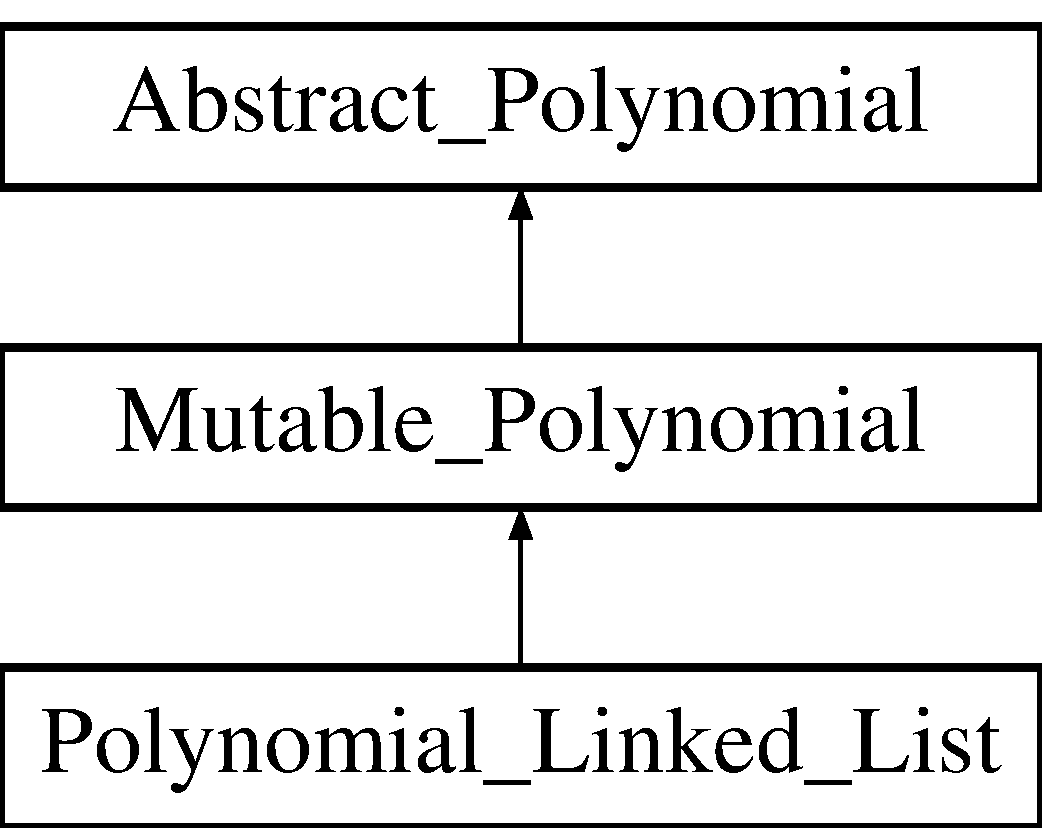
\includegraphics[height=3.000000cm]{group__polygroup}
\end{center}
\end{figure}
\subsubsection*{Public Member Functions}
\begin{Indent}\textbf{ Construction}\par
\begin{DoxyCompactItemize}
\item 
\mbox{\Hypertarget{group__polygroup_ab663800f31484a5d55ec9363e7669f56}\label{group__polygroup_ab663800f31484a5d55ec9363e7669f56}} 
{\bfseries Double\+\_\+\+Buffered\+\_\+\+Polynomial} (\hyperlink{group__polygroup_class_polynomial___ring}{Polynomial\+\_\+\+Ring} \&\hyperlink{group__polygroup_a551ade20b7dcd96c227dd0401f6ffbbe}{R}, \hyperlink{group__orderinggroup_class_monomial___ordering}{Monomial\+\_\+\+Ordering} $\ast$order=generic\+\_\+grevlex\+\_\+ptr)
\item 
\mbox{\Hypertarget{group__polygroup_ace854a5e7d0fac35ad2d9469a34656a7}\label{group__polygroup_ace854a5e7d0fac35ad2d9469a34656a7}} 
{\bfseries Double\+\_\+\+Buffered\+\_\+\+Polynomial} (\hyperlink{group__polygroup_class_abstract___polynomial}{Abstract\+\_\+\+Polynomial} const \&p)
\end{DoxyCompactItemize}
\end{Indent}
\begin{Indent}\textbf{ Destruction}\par
\begin{DoxyCompactItemize}
\item 
\mbox{\Hypertarget{group__polygroup_a61b7620ea7b3b7ba3db0b96065458166}\label{group__polygroup_a61b7620ea7b3b7ba3db0b96065458166}} 
{\bfseries $\sim$\+Double\+\_\+\+Buffered\+\_\+\+Polynomial} ()
\end{DoxyCompactItemize}
\end{Indent}
\begin{Indent}\textbf{ Basic properties}\par
\begin{DoxyCompactItemize}
\item 
\mbox{\Hypertarget{group__polygroup_ac858fe599295a6b20c2a2df1ead74068}\label{group__polygroup_ac858fe599295a6b20c2a2df1ead74068}} 
virtual \hyperlink{group__polygroup_class_monomial}{Monomial} \& \hyperlink{group__polygroup_ac858fe599295a6b20c2a2df1ead74068}{leading\+\_\+monomial} () const override
\begin{DoxyCompactList}\small\item\em leading monomial -- call after \hyperlink{group__polygroup_a41e751eee1614e26ebba39a9f81f7993}{sort\+\_\+by\+\_\+order()}! \end{DoxyCompactList}\item 
\mbox{\Hypertarget{group__polygroup_a48c1d3abec70bb53e148ee7e14480ad6}\label{group__polygroup_a48c1d3abec70bb53e148ee7e14480ad6}} 
virtual \hyperlink{group___fields_group_class_prime___field___element}{Prime\+\_\+\+Field\+\_\+\+Element} \hyperlink{group__polygroup_a48c1d3abec70bb53e148ee7e14480ad6}{leading\+\_\+coefficient} () const override
\begin{DoxyCompactList}\small\item\em leading coefficient -- call after \hyperlink{group__polygroup_a41e751eee1614e26ebba39a9f81f7993}{sort\+\_\+by\+\_\+order()}! \end{DoxyCompactList}\item 
\mbox{\Hypertarget{group__polygroup_a05caa373c56753d535caf24f4f2005df}\label{group__polygroup_a05caa373c56753d535caf24f4f2005df}} 
virtual unsigned \hyperlink{group__polygroup_a05caa373c56753d535caf24f4f2005df}{length} () const override
\begin{DoxyCompactList}\small\item\em number of monomials \end{DoxyCompactList}\item 
\mbox{\Hypertarget{group__polygroup_a1a4c51dd399e62884acfd6f935057463}\label{group__polygroup_a1a4c51dd399e62884acfd6f935057463}} 
virtual bool \hyperlink{group__polygroup_a1a4c51dd399e62884acfd6f935057463}{is\+\_\+zero} () const override
\begin{DoxyCompactList}\small\item\em is this polynomial zero? \end{DoxyCompactList}\item 
\mbox{\Hypertarget{group__polygroup_af01f234c0897a5a01590f9b35e7e566f}\label{group__polygroup_af01f234c0897a5a01590f9b35e7e566f}} 
virtual bool \hyperlink{group__polygroup_af01f234c0897a5a01590f9b35e7e566f}{can\+\_\+reduce} (\hyperlink{group__polygroup_class_abstract___polynomial}{Abstract\+\_\+\+Polynomial} \&other) const override
\begin{DoxyCompactList}\small\item\em can {\ttfamily this} reduce {\ttfamily other}? \end{DoxyCompactList}\item 
\mbox{\Hypertarget{group__polygroup_a9485263fbd2bf13b0eb01926e6439238}\label{group__polygroup_a9485263fbd2bf13b0eb01926e6439238}} 
virtual \hyperlink{group__polygroup_class_double___buffered___polynomial}{Double\+\_\+\+Buffered\+\_\+\+Polynomial} $\ast$ \hyperlink{group__polygroup_a9485263fbd2bf13b0eb01926e6439238}{zero\+\_\+polynomial} () const override
\begin{DoxyCompactList}\small\item\em zero polynomial of this type \end{DoxyCompactList}\item 
virtual void \hyperlink{group__polygroup_aa81be797dcced4e663d3fe54f6501ed6}{set\+\_\+monomial\+\_\+ordering} (const \hyperlink{group__orderinggroup_class_monomial___ordering}{Monomial\+\_\+\+Ordering} $\ast$order, bool sort\+\_\+anew=true) override
\begin{DoxyCompactList}\small\item\em set the monomial ordering and sort the polynomials (optionally, but by default) \end{DoxyCompactList}\end{DoxyCompactItemize}
\end{Indent}
\begin{Indent}\textbf{ Computation}\par
\begin{DoxyCompactItemize}
\item 
\mbox{\Hypertarget{group__polygroup_af210793e13c89388c3704d27bbf96516}\label{group__polygroup_af210793e13c89388c3704d27bbf96516}} 
virtual \hyperlink{group__polygroup_class_double___buffered___polynomial}{Double\+\_\+\+Buffered\+\_\+\+Polynomial} $\ast$ \hyperlink{group__polygroup_af210793e13c89388c3704d27bbf96516}{monomial\+\_\+multiple} (const \hyperlink{group__polygroup_class_monomial}{Monomial} \&t) const override
\begin{DoxyCompactList}\small\item\em multiple of this and u \end{DoxyCompactList}\item 
\mbox{\Hypertarget{group__polygroup_a7d434fba3c5a5f8eb1c6ebd2dfd24eac}\label{group__polygroup_a7d434fba3c5a5f8eb1c6ebd2dfd24eac}} 
virtual \hyperlink{group__polygroup_class_double___buffered___polynomial}{Double\+\_\+\+Buffered\+\_\+\+Polynomial} $\ast$ \hyperlink{group__polygroup_a7d434fba3c5a5f8eb1c6ebd2dfd24eac}{scalar\+\_\+multiple} (const \hyperlink{group___fields_group_class_prime___field___element}{Prime\+\_\+\+Field\+\_\+\+Element} \&c) const override
\begin{DoxyCompactList}\small\item\em multiple of this and c \end{DoxyCompactList}\item 
\mbox{\Hypertarget{group__polygroup_ad30266ecf9eb2845b29a673e30d33b77}\label{group__polygroup_ad30266ecf9eb2845b29a673e30d33b77}} 
virtual \hyperlink{group__polygroup_class_mutable___polynomial}{Mutable\+\_\+\+Polynomial} \& \hyperlink{group__polygroup_ad30266ecf9eb2845b29a673e30d33b77}{operator+=} (const \hyperlink{group__polygroup_class_abstract___polynomial}{Abstract\+\_\+\+Polynomial} \&p) override
\begin{DoxyCompactList}\small\item\em add another polynomial \end{DoxyCompactList}\item 
\mbox{\Hypertarget{group__polygroup_ac8c06c72eb6242460aeb00810abb0d2d}\label{group__polygroup_ac8c06c72eb6242460aeb00810abb0d2d}} 
virtual \hyperlink{group__polygroup_class_mutable___polynomial}{Mutable\+\_\+\+Polynomial} \& \hyperlink{group__polygroup_ac8c06c72eb6242460aeb00810abb0d2d}{operator-\/=} (const \hyperlink{group__polygroup_class_abstract___polynomial}{Abstract\+\_\+\+Polynomial} \&p) override
\begin{DoxyCompactList}\small\item\em subtract another polynomial \end{DoxyCompactList}\item 
\mbox{\Hypertarget{group__polygroup_a4536176cfe316974e14d3273ac9f9462}\label{group__polygroup_a4536176cfe316974e14d3273ac9f9462}} 
virtual void \hyperlink{group__polygroup_a4536176cfe316974e14d3273ac9f9462}{add\+\_\+polynomial\+\_\+multiple} (const \hyperlink{group___fields_group_class_prime___field___element}{Prime\+\_\+\+Field\+\_\+\+Element} \&a, const \hyperlink{group__polygroup_class_monomial}{Monomial} \&u, const \hyperlink{group__polygroup_class_abstract___polynomial}{Abstract\+\_\+\+Polynomial} \&p, bool subtract) override
\begin{DoxyCompactList}\small\item\em add monomial multiple of other \end{DoxyCompactList}\item 
virtual void \hyperlink{group__polygroup_a41e751eee1614e26ebba39a9f81f7993}{sort\+\_\+by\+\_\+order} () override
\begin{DoxyCompactList}\small\item\em sort according to the leading monomial's ordering \end{DoxyCompactList}\end{DoxyCompactItemize}
\end{Indent}
\begin{Indent}\textbf{ Iteration}\par
\begin{DoxyCompactItemize}
\item 
\mbox{\Hypertarget{group__polygroup_a224ae300d1789243ca05e4413c473a6f}\label{group__polygroup_a224ae300d1789243ca05e4413c473a6f}} 
virtual \hyperlink{group___iterator_group_class_d_b___polynomial___iterator}{D\+B\+\_\+\+Polynomial\+\_\+\+Iterator} $\ast$ \hyperlink{group__polygroup_a224ae300d1789243ca05e4413c473a6f}{new\+\_\+iterator} () const override
\begin{DoxyCompactList}\small\item\em An iterator that poses no risk of modifying the polynomial. \end{DoxyCompactList}\item 
\mbox{\Hypertarget{group__polygroup_aabbde4f088511cb480e959eaac056784}\label{group__polygroup_aabbde4f088511cb480e959eaac056784}} 
virtual \hyperlink{group___iterator_group_class_d_b___polynomial___iterator}{D\+B\+\_\+\+Polynomial\+\_\+\+Iterator} $\ast$ \hyperlink{group__polygroup_aabbde4f088511cb480e959eaac056784}{new\+\_\+mutable\+\_\+iterator} () override
\begin{DoxyCompactList}\small\item\em An iterator that may modify the current position. \end{DoxyCompactList}\item 
\mbox{\Hypertarget{group__polygroup_a85169b0b1146537bb69127f3c1a866ff}\label{group__polygroup_a85169b0b1146537bb69127f3c1a866ff}} 
virtual \hyperlink{group___iterator_group_class_polynomial___iterator}{Polynomial\+\_\+\+Iterator} $\ast$ \hyperlink{group__polygroup_a85169b0b1146537bb69127f3c1a866ff}{begin} () const override
\begin{DoxyCompactList}\small\item\em returns an iterator to the polynomial's leading monomial \end{DoxyCompactList}\item 
\mbox{\Hypertarget{group__polygroup_ad89a902fa53246364fbef37eefa44080}\label{group__polygroup_ad89a902fa53246364fbef37eefa44080}} 
virtual \hyperlink{group___iterator_group_class_polynomial___iterator}{Polynomial\+\_\+\+Iterator} $\ast$ \hyperlink{group__polygroup_ad89a902fa53246364fbef37eefa44080}{end} () const override
\begin{DoxyCompactList}\small\item\em iterator to last monomial \end{DoxyCompactList}\end{DoxyCompactItemize}
\end{Indent}
\begin{Indent}\textbf{ Modification}\par
\begin{DoxyCompactItemize}
\item 
\mbox{\Hypertarget{group__polygroup_a5bcb9f095148d20d1f428f75e8bd081d}\label{group__polygroup_a5bcb9f095148d20d1f428f75e8bd081d}} 
virtual void \hyperlink{group__polygroup_a5bcb9f095148d20d1f428f75e8bd081d}{add\+\_\+last} (const \hyperlink{group___fields_group_class_prime___field___element}{Prime\+\_\+\+Field\+\_\+\+Element} \&a, const \hyperlink{group__polygroup_class_monomial}{Monomial} \&t) override
\begin{DoxyCompactList}\small\item\em Attach a new monomial to the tail -- check that it belongs at tail! \end{DoxyCompactList}\item 
\mbox{\Hypertarget{group__polygroup_a4414c7a72f980efac7b794525151b653}\label{group__polygroup_a4414c7a72f980efac7b794525151b653}} 
virtual \hyperlink{group__polygroup_class_polynomial___linked___list}{Polynomial\+\_\+\+Linked\+\_\+\+List} $\ast$ \hyperlink{group__polygroup_a4414c7a72f980efac7b794525151b653}{detach\+\_\+head} () override
\begin{DoxyCompactList}\small\item\em Remove and return the head. \end{DoxyCompactList}\end{DoxyCompactItemize}
\end{Indent}
\subsubsection*{Protected Member Functions}
\begin{Indent}\textbf{ Buffering}\par
\begin{DoxyCompactItemize}
\item 
\mbox{\Hypertarget{group__polygroup_a399d8bc13840f21ab8a1b8c844053eb9}\label{group__polygroup_a399d8bc13840f21ab8a1b8c844053eb9}} 
bool \hyperlink{group__polygroup_a399d8bc13840f21ab8a1b8c844053eb9}{test\+\_\+buffer} (unsigned b, unsigned n)
\begin{DoxyCompactList}\small\item\em {\ttfamily true} iff buffer {\ttfamily b} has space to hold {\ttfamily n} elements; expand other buffer if not. \end{DoxyCompactList}\item 
void \hyperlink{group__polygroup_acd9235d4fe5a56a3a0842a80b4efbdbb}{expand\+\_\+buffer} (unsigned b, unsigned n)
\begin{DoxyCompactList}\small\item\em Expand buffer {\ttfamily b} to hold $ 2n $ elements. \end{DoxyCompactList}\end{DoxyCompactItemize}
\end{Indent}
\subsubsection*{Friends}
\begin{DoxyCompactItemize}
\item 
\mbox{\Hypertarget{group__polygroup_aea7290ecfb1e468c20192be43af46a96}\label{group__polygroup_aea7290ecfb1e468c20192be43af46a96}} 
class \hyperlink{group__polygroup_aea7290ecfb1e468c20192be43af46a96}{D\+B\+\_\+\+Polynomial\+\_\+\+Iterator}
\begin{DoxyCompactList}\small\item\em to iterate over {\ttfamily this} and possibly change it \end{DoxyCompactList}\end{DoxyCompactItemize}
\subsection*{Additional Inherited Members}


\paragraph{Member Function Documentation}
\mbox{\Hypertarget{group__polygroup_acd9235d4fe5a56a3a0842a80b4efbdbb}\label{group__polygroup_acd9235d4fe5a56a3a0842a80b4efbdbb}} 
\index{Double\+\_\+\+Buffered\+\_\+\+Polynomial@{Double\+\_\+\+Buffered\+\_\+\+Polynomial}!expand\+\_\+buffer@{expand\+\_\+buffer}}
\index{expand\+\_\+buffer@{expand\+\_\+buffer}!Double\+\_\+\+Buffered\+\_\+\+Polynomial@{Double\+\_\+\+Buffered\+\_\+\+Polynomial}}
\subparagraph{\texorpdfstring{expand\+\_\+buffer()}{expand\_buffer()}}
{\footnotesize\ttfamily void Double\+\_\+\+Buffered\+\_\+\+Polynomial\+::expand\+\_\+buffer (\begin{DoxyParamCaption}\item[{unsigned}]{b,  }\item[{unsigned}]{n }\end{DoxyParamCaption})\hspace{0.3cm}{\ttfamily [inline]}, {\ttfamily [protected]}}



Expand buffer {\ttfamily b} to hold $ 2n $ elements. 


\begin{DoxyParams}{Parameters}
{\em b} & the buffer to expand \\
\hline
{\em n} & number of monomials you'd like it to hold now\\
\hline
\end{DoxyParams}
This does {\itshape not} test to see if the space is already available. 

Definition at line 214 of file polynomial\+\_\+double\+\_\+buffered.\+hpp.

\mbox{\Hypertarget{group__polygroup_aa81be797dcced4e663d3fe54f6501ed6}\label{group__polygroup_aa81be797dcced4e663d3fe54f6501ed6}} 
\index{Double\+\_\+\+Buffered\+\_\+\+Polynomial@{Double\+\_\+\+Buffered\+\_\+\+Polynomial}!set\+\_\+monomial\+\_\+ordering@{set\+\_\+monomial\+\_\+ordering}}
\index{set\+\_\+monomial\+\_\+ordering@{set\+\_\+monomial\+\_\+ordering}!Double\+\_\+\+Buffered\+\_\+\+Polynomial@{Double\+\_\+\+Buffered\+\_\+\+Polynomial}}
\subparagraph{\texorpdfstring{set\+\_\+monomial\+\_\+ordering()}{set\_monomial\_ordering()}}
{\footnotesize\ttfamily void Double\+\_\+\+Buffered\+\_\+\+Polynomial\+::set\+\_\+monomial\+\_\+ordering (\begin{DoxyParamCaption}\item[{const \hyperlink{group__orderinggroup_class_monomial___ordering}{Monomial\+\_\+\+Ordering} $\ast$}]{order,  }\item[{bool}]{sort\+\_\+anew = {\ttfamily true} }\end{DoxyParamCaption})\hspace{0.3cm}{\ttfamily [override]}, {\ttfamily [virtual]}}



set the monomial ordering and sort the polynomials (optionally, but by default) 


\begin{DoxyParams}{Parameters}
{\em order} & new monomial ordering \\
\hline
{\em sort\+\_\+anew} & whether to sort the polynomial anew \\
\hline
\end{DoxyParams}
\begin{DoxyWarning}{Warning}
In most cases you will want to sort anew {\itshape immediately} after setting the ordering. Otherwise, the monomials may be in the wrong order! That is therefore the default behavior of this function, but in case you don't want to sort, that option is provided. 
\end{DoxyWarning}


Implements \hyperlink{group__polygroup_a12e023570eb675343c4b7ed635a031dc}{Abstract\+\_\+\+Polynomial}.



Definition at line 145 of file polynomial\+\_\+double\+\_\+buffered.\+cpp.

\mbox{\Hypertarget{group__polygroup_a41e751eee1614e26ebba39a9f81f7993}\label{group__polygroup_a41e751eee1614e26ebba39a9f81f7993}} 
\index{Double\+\_\+\+Buffered\+\_\+\+Polynomial@{Double\+\_\+\+Buffered\+\_\+\+Polynomial}!sort\+\_\+by\+\_\+order@{sort\+\_\+by\+\_\+order}}
\index{sort\+\_\+by\+\_\+order@{sort\+\_\+by\+\_\+order}!Double\+\_\+\+Buffered\+\_\+\+Polynomial@{Double\+\_\+\+Buffered\+\_\+\+Polynomial}}
\subparagraph{\texorpdfstring{sort\+\_\+by\+\_\+order()}{sort\_by\_order()}}
{\footnotesize\ttfamily void Double\+\_\+\+Buffered\+\_\+\+Polynomial\+::sort\+\_\+by\+\_\+order (\begin{DoxyParamCaption}{ }\end{DoxyParamCaption})\hspace{0.3cm}{\ttfamily [override]}, {\ttfamily [virtual]}}



sort according to the leading monomial's ordering 

Note that it makes sense to sort even \hyperlink{group__polygroup_class_constant___polynomial}{Constant\+\_\+\+Polynomial}'s, as it is not the polynomial that changes, only the order of its monomials. 

Implements \hyperlink{group__polygroup_a1fcdd29c324c660ea935197c39e682f2}{Abstract\+\_\+\+Polynomial}.



Definition at line 346 of file polynomial\+\_\+double\+\_\+buffered.\+cpp.

\index{Indeterminate@{Indeterminate}}\label{class_indeterminate}
\Hypertarget{group__polygroup_class_indeterminate}
\subsubsection{class Indeterminate}
Implementation of indeterminates, for easier building of polynomials. 

\begin{DoxyAuthor}{Author}
John Perry
\end{DoxyAuthor}
\begin{DoxyDate}{Date}
2016
\end{DoxyDate}
The main purpose of this class is to help make it easier to build polynomials. It is not especially useful otherwise, and is highly inefficient. However, it makes the following possible\+: 
\begin{DoxyCode}
\hyperlink{group___fields_group_class_prime___field}{Prime\_Field} F = \hyperlink{group___fields_group_class_prime___field}{Prime\_Field}(43);
\textcolor{keywordtype}{string} var\_names [] = \{ \textcolor{stringliteral}{"x"}, \textcolor{stringliteral}{"y"} \};
P = \hyperlink{group__polygroup_class_polynomial___ring}{Polynomial\_Ring}(2, F, var\_names);
\hyperlink{group__polygroup_class_indeterminate}{Indeterminate} x(\hyperlink{group__polygroup_a78f5339712602f11e29a091d228032c4}{R}, 0);
\hyperlink{group__polygroup_class_indeterminate}{Indeterminate} y(\hyperlink{group__polygroup_a78f5339712602f11e29a091d228032c4}{R}, 1);
\hyperlink{group__polygroup_class_monomial}{Monomial} x3y = (x^3) * (x*y);
x3y.\hyperlink{group__polygroup_a34143922dd6ce2d44a62777a8948bf97}{printlncout}();
\end{DoxyCode}
 {$\dots$}and the result should be $x^3y$. Alternately, you could do\+: 
\begin{DoxyCode}
\hyperlink{group__polygroup_class_indeterminate}{Indeterminate} * X = P.indeterminates();
\hyperlink{group__polygroup_class_monomial}{Monomial} x3y = (X[0]^3) * (X[0]*X[1]);
x3y.\hyperlink{group__polygroup_a34143922dd6ce2d44a62777a8948bf97}{printlncout}();
free(X);
\end{DoxyCode}
 {$\dots$}with the same result. Just be careful in the second case to destroy the evidence. \begin{Desc}
\item[Examples\+: ]\par
\hyperlink{test_monomials_8cpp-example}{test\+\_\+monomials.\+cpp}.\end{Desc}


Definition at line 63 of file indeterminate.\+hpp.

\subsubsection*{Public Member Functions}
\begin{Indent}\textbf{ Construction}\par
\begin{DoxyCompactItemize}
\item 
\mbox{\Hypertarget{group__polygroup_a69cacbaf1f95b735ae1126de93f1da5c}\label{group__polygroup_a69cacbaf1f95b735ae1126de93f1da5c}} 
\hyperlink{group__polygroup_a69cacbaf1f95b735ae1126de93f1da5c}{Indeterminate} (\hyperlink{group__polygroup_class_polynomial___ring}{Polynomial\+\_\+\+Ring} \&P, N\+V\+A\+R\+\_\+\+T\+Y\+PE xi)
\begin{DoxyCompactList}\small\item\em {\ttfamily this} will correspond to the {\ttfamily xi}th indeterminate of {\ttfamily P}. \end{DoxyCompactList}\item 
\mbox{\Hypertarget{group__polygroup_affe3146cd68726d8a7f7cb1e70bc19fb}\label{group__polygroup_affe3146cd68726d8a7f7cb1e70bc19fb}} 
\hyperlink{group__polygroup_affe3146cd68726d8a7f7cb1e70bc19fb}{Indeterminate} (const \hyperlink{group__polygroup_class_indeterminate}{Indeterminate} \&other)
\begin{DoxyCompactList}\small\item\em copy constructor \end{DoxyCompactList}\item 
\mbox{\Hypertarget{group__polygroup_ac2540ce0eecc8b82afd5d6742e27d6e4}\label{group__polygroup_ac2540ce0eecc8b82afd5d6742e27d6e4}} 
\hyperlink{group__polygroup_class_indeterminate}{Indeterminate} \& {\bfseries operator=} (const \hyperlink{group__polygroup_class_indeterminate}{Indeterminate} \&other)
\end{DoxyCompactItemize}
\end{Indent}
\begin{Indent}\textbf{ Basic properties}\par
\begin{DoxyCompactItemize}
\item 
\mbox{\Hypertarget{group__polygroup_ab3e27b16e7da9518ccba7f91969cd88f}\label{group__polygroup_ab3e27b16e7da9518ccba7f91969cd88f}} 
\hyperlink{group__polygroup_class_polynomial___ring}{Polynomial\+\_\+\+Ring} \& \hyperlink{group__polygroup_ab3e27b16e7da9518ccba7f91969cd88f}{base\+\_\+ring} ()
\begin{DoxyCompactList}\small\item\em the \hyperlink{group__polygroup_class_polynomial___ring}{Polynomial\+\_\+\+Ring} {\ttfamily this} lives in \end{DoxyCompactList}\item 
\mbox{\Hypertarget{group__polygroup_acb2070ec4ddcaca8ded1ff14856cf966}\label{group__polygroup_acb2070ec4ddcaca8ded1ff14856cf966}} 
N\+V\+A\+R\+\_\+\+T\+Y\+PE \hyperlink{group__polygroup_acb2070ec4ddcaca8ded1ff14856cf966}{index\+\_\+in\+\_\+ring} ()
\begin{DoxyCompactList}\small\item\em which variable in \hyperlink{group__polygroup_ab3e27b16e7da9518ccba7f91969cd88f}{base\+\_\+ring()} {\ttfamily this} is \end{DoxyCompactList}\end{DoxyCompactItemize}
\end{Indent}
\begin{Indent}\textbf{ Computation}\par
\begin{DoxyCompactItemize}
\item 
\mbox{\Hypertarget{group__polygroup_a91dbca8f634ff05a13a168b5cd2e258e}\label{group__polygroup_a91dbca8f634ff05a13a168b5cd2e258e}} 
\hyperlink{group__polygroup_class_monomial}{Monomial} \hyperlink{group__polygroup_a91dbca8f634ff05a13a168b5cd2e258e}{operator$^\wedge$} (E\+X\+P\+\_\+\+T\+Y\+PE a)
\begin{DoxyCompactList}\small\item\em returns {\ttfamily this} to the {\ttfamily a}th power \end{DoxyCompactList}\item 
\mbox{\Hypertarget{group__polygroup_a969b2a98b105e719d83e3036f8872653}\label{group__polygroup_a969b2a98b105e719d83e3036f8872653}} 
\hyperlink{group__polygroup_class_monomial}{Monomial} \hyperlink{group__polygroup_a969b2a98b105e719d83e3036f8872653}{operator$\ast$} (\hyperlink{group__polygroup_class_indeterminate}{Indeterminate} y)
\begin{DoxyCompactList}\small\item\em returns the product of {\ttfamily this} and {\ttfamily y} \end{DoxyCompactList}\item 
\mbox{\Hypertarget{group__polygroup_a936f26303c8f00f0cfe1251a29432550}\label{group__polygroup_a936f26303c8f00f0cfe1251a29432550}} 
\hyperlink{group__polygroup_class_monomial}{Monomial} \hyperlink{group__polygroup_a936f26303c8f00f0cfe1251a29432550}{operator$\ast$} (\hyperlink{group__polygroup_class_monomial}{Monomial} t)
\begin{DoxyCompactList}\small\item\em returns the product of {\ttfamily this} and {\ttfamily t} \end{DoxyCompactList}\end{DoxyCompactItemize}
\end{Indent}
\subsubsection*{Protected Attributes}
\begin{DoxyCompactItemize}
\item 
\mbox{\Hypertarget{group__polygroup_aab06276a83206026ef44fb6249971796}\label{group__polygroup_aab06276a83206026ef44fb6249971796}} 
N\+V\+A\+R\+\_\+\+T\+Y\+PE \hyperlink{group__polygroup_aab06276a83206026ef44fb6249971796}{i}
\begin{DoxyCompactList}\small\item\em which indeterminate in {\ttfamily R} {\ttfamily this} is \end{DoxyCompactList}\item 
\mbox{\Hypertarget{group__polygroup_a78f5339712602f11e29a091d228032c4}\label{group__polygroup_a78f5339712602f11e29a091d228032c4}} 
\hyperlink{group__polygroup_class_polynomial___ring}{Polynomial\+\_\+\+Ring} $\ast$ \hyperlink{group__polygroup_a78f5339712602f11e29a091d228032c4}{R}
\begin{DoxyCompactList}\small\item\em the ring {\ttfamily this} lives in \end{DoxyCompactList}\end{DoxyCompactItemize}
\subsubsection*{Friends}
\begin{Indent}\textbf{ I/O}\par
\begin{DoxyCompactItemize}
\item 
\mbox{\Hypertarget{group__polygroup_a0fbbf892bdfabc97b41ec7e486e83125}\label{group__polygroup_a0fbbf892bdfabc97b41ec7e486e83125}} 
ostream \& \hyperlink{group__polygroup_a0fbbf892bdfabc97b41ec7e486e83125}{operator$<$$<$} (ostream \&, \hyperlink{group__polygroup_class_indeterminate}{Indeterminate} \&)
\begin{DoxyCompactList}\small\item\em prints {\ttfamily this} with the appropriate name \end{DoxyCompactList}\end{DoxyCompactItemize}
\end{Indent}
\index{Monomial@{Monomial}}\label{class_monomial}
\Hypertarget{group__polygroup_class_monomial}
\subsubsection{class Monomial}
Implementation of monomials. 

\begin{DoxyAuthor}{Author}
John Perry 
\end{DoxyAuthor}
\begin{DoxyDate}{Date}
2015
\end{DoxyDate}
A monomial is a product of powers, for instance $x_1^2x_3$. (We do not include coefficients in our definition of monomials.) This class encapsulates basic monomial functionality necessary for computing Gr\"{o}bner bases.

\begin{DoxyWarning}{Warning}
When initializing an array of {\ttfamily \hyperlink{group__polygroup_class_monomial}{Monomial}} , be sure to use the initialization functions to format and allocate space.

Any monomial requires that you specify a number of variables. At the present time, the limit on this is 64 (for the sake of masking; though an earlier verison of the code did not have this limit). Most operations require that the number of variables be the same, but the code does not check for this. For what I am designing this for, this is acceptable, but if you intend to work with monomials that contain a different number of variables, check to make sure that any monomial arithmetic involves monomials with the same number of variables. 
\end{DoxyWarning}
\begin{Desc}
\item[Examples\+: ]\par
\hyperlink{test_4by4_8cpp-example}{test\+\_\+4by4.\+cpp}, \hyperlink{test_cab_es1_8cpp-example}{test\+\_\+cab\+\_\+es1.\+cpp}, \hyperlink{test_cab_es2_8cpp-example}{test\+\_\+cab\+\_\+es2.\+cpp}, \hyperlink{test_cab_es4_8cpp-example}{test\+\_\+cab\+\_\+es4.\+cpp}, \hyperlink{test_cab_es5_8cpp-example}{test\+\_\+cab\+\_\+es5.\+cpp}, \hyperlink{test_cab_es6_8cpp-example}{test\+\_\+cab\+\_\+es6.\+cpp}, \hyperlink{test_cab_es9_8cpp-example}{test\+\_\+cab\+\_\+es9.\+cpp}, \hyperlink{test_cyclic4_8cpp-example}{test\+\_\+cyclic4.\+cpp}, \hyperlink{test_monomials_8cpp-example}{test\+\_\+monomials.\+cpp}, and \hyperlink{user_interface_8cpp-example}{user\+\_\+interface.\+cpp}.\end{Desc}


Definition at line 69 of file monomial.\+hpp.

\subsubsection*{Public Member Functions}
\begin{Indent}\textbf{ Construction}\par
\begin{DoxyCompactItemize}
\item 
\mbox{\Hypertarget{group__polygroup_a7d50554f29ff84177270316088772397}\label{group__polygroup_a7d50554f29ff84177270316088772397}} 
void \hyperlink{group__polygroup_a7d50554f29ff84177270316088772397}{common\+\_\+initialization} (const \hyperlink{group__orderinggroup_class_monomial___ordering}{Monomial\+\_\+\+Ordering} $\ast$ord=nullptr)
\begin{DoxyCompactList}\small\item\em things all {\ttfamily \hyperlink{group__polygroup_class_monomial}{Monomial}} initializers must do \end{DoxyCompactList}\item 
\mbox{\Hypertarget{group__polygroup_a1103a9a7e8d60147a1e00a1bd23bfea3}\label{group__polygroup_a1103a9a7e8d60147a1e00a1bd23bfea3}} 
void \hyperlink{group__polygroup_a1103a9a7e8d60147a1e00a1bd23bfea3}{initialize\+\_\+exponents} (N\+V\+A\+R\+\_\+\+T\+Y\+PE number\+\_\+of\+\_\+vars)
\begin{DoxyCompactList}\small\item\em allocates memory for exponents This is useful when you want to allocate an array of monomials. \end{DoxyCompactList}\item 
\mbox{\Hypertarget{group__polygroup_a471eab4cf0ce40225a1b8210513ad9e4}\label{group__polygroup_a471eab4cf0ce40225a1b8210513ad9e4}} 
void \hyperlink{group__polygroup_a471eab4cf0ce40225a1b8210513ad9e4}{deinitialize} ()
\begin{DoxyCompactList}\small\item\em deallocates memory for exponents This is useful when you want to deallocate an array of monomials. \end{DoxyCompactList}\item 
\mbox{\Hypertarget{group__polygroup_a6f28aa6d15979b018003908937155052}\label{group__polygroup_a6f28aa6d15979b018003908937155052}} 
void \hyperlink{group__polygroup_a6f28aa6d15979b018003908937155052}{set\+\_\+exponent} (N\+V\+A\+R\+\_\+\+T\+Y\+PE i, D\+E\+G\+\_\+\+T\+Y\+PE e)
\begin{DoxyCompactList}\small\item\em change $i$th exponent to $e$ \end{DoxyCompactList}\item 
\mbox{\Hypertarget{group__polygroup_a3c710f9d6f7c7e0addc2779a037042dd}\label{group__polygroup_a3c710f9d6f7c7e0addc2779a037042dd}} 
\hyperlink{group__polygroup_a3c710f9d6f7c7e0addc2779a037042dd}{Monomial} (N\+V\+A\+R\+\_\+\+T\+Y\+PE number\+\_\+of\+\_\+vars, const \hyperlink{group__orderinggroup_class_monomial___ordering}{Monomial\+\_\+\+Ordering} $\ast$order=generic\+\_\+grevlex\+\_\+ptr)
\begin{DoxyCompactList}\small\item\em The first constructor is equivalent to instantiating 1. \end{DoxyCompactList}\item 
\mbox{\Hypertarget{group__polygroup_ad6968b542cf22f8bc24053fb48782dcc}\label{group__polygroup_ad6968b542cf22f8bc24053fb48782dcc}} 
\hyperlink{group__polygroup_ad6968b542cf22f8bc24053fb48782dcc}{Monomial} (const \hyperlink{group__polygroup_class_monomial}{Monomial} \&other)
\begin{DoxyCompactList}\small\item\em Copy constructor, allocates new space for exponents. \end{DoxyCompactList}\item 
\hyperlink{group__polygroup_a8b9c7bc9d5b286adb11ccc39471b00c4}{Monomial} (initializer\+\_\+list$<$ E\+X\+P\+\_\+\+T\+Y\+PE $>$ powers, const \hyperlink{group__orderinggroup_class_monomial___ordering}{Monomial\+\_\+\+Ordering} $\ast$order=generic\+\_\+grevlex\+\_\+ptr)
\begin{DoxyCompactList}\small\item\em Constructor from initializer list. \end{DoxyCompactList}\item 
\hyperlink{group__polygroup_a85d91b1a13592c849394c26c5ad294d8}{Monomial} (N\+V\+A\+R\+\_\+\+T\+Y\+PE size, const E\+X\+P\+\_\+\+T\+Y\+PE $\ast$powers, const \hyperlink{group__orderinggroup_class_monomial___ordering}{Monomial\+\_\+\+Ordering} $\ast$order=generic\+\_\+grevlex\+\_\+ptr)
\begin{DoxyCompactList}\small\item\em Constructor from array of exponents. \end{DoxyCompactList}\end{DoxyCompactItemize}
\end{Indent}
\begin{Indent}\textbf{ Destruction}\par
\begin{DoxyCompactItemize}
\item 
\mbox{\Hypertarget{group__polygroup_a7c56cfe0292638732d60169d960f877c}\label{group__polygroup_a7c56cfe0292638732d60169d960f877c}} 
\hyperlink{group__polygroup_a7c56cfe0292638732d60169d960f877c}{$\sim$\+Monomial} ()
\begin{DoxyCompactList}\small\item\em Destructor deallocates exponents. \end{DoxyCompactList}\end{DoxyCompactItemize}
\end{Indent}
\begin{Indent}\textbf{ Basic properties}\par
{\em The following functions give information about the monomial, but do not modify it. }\begin{DoxyCompactItemize}
\item 
\mbox{\Hypertarget{group__polygroup_a4ade87fb2cae33669c66c7b23819ba57}\label{group__polygroup_a4ade87fb2cae33669c66c7b23819ba57}} 
N\+V\+A\+R\+\_\+\+T\+Y\+PE \hyperlink{group__polygroup_a4ade87fb2cae33669c66c7b23819ba57}{num\+\_\+vars} () const
\begin{DoxyCompactList}\small\item\em number of variables \end{DoxyCompactList}\item 
\mbox{\Hypertarget{group__polygroup_aa1508ad890693aee2f5c35e156f12e83}\label{group__polygroup_aa1508ad890693aee2f5c35e156f12e83}} 
bool \hyperlink{group__polygroup_aa1508ad890693aee2f5c35e156f12e83}{is\+\_\+one} () const
\begin{DoxyCompactList}\small\item\em all exponents 0? \end{DoxyCompactList}\item 
\mbox{\Hypertarget{group__polygroup_a817508c95fe721c56c78d91975b8416b}\label{group__polygroup_a817508c95fe721c56c78d91975b8416b}} 
D\+E\+G\+\_\+\+T\+Y\+PE \hyperlink{group__polygroup_a817508c95fe721c56c78d91975b8416b}{degree} (N\+V\+A\+R\+\_\+\+T\+Y\+PE i) const
\begin{DoxyCompactList}\small\item\em Degree of $i$th variable. \end{DoxyCompactList}\item 
\mbox{\Hypertarget{group__polygroup_ab3c18ba0fe7442e07d630bddea3469b5}\label{group__polygroup_ab3c18ba0fe7442e07d630bddea3469b5}} 
D\+E\+G\+\_\+\+T\+Y\+PE \hyperlink{group__polygroup_ab3c18ba0fe7442e07d630bddea3469b5}{operator\mbox{[}$\,$\mbox{]}} (N\+V\+A\+R\+\_\+\+T\+Y\+PE i) const
\begin{DoxyCompactList}\small\item\em Degree of $i$th variable. Synonymous with \hyperlink{group__polygroup_a817508c95fe721c56c78d91975b8416b}{degree()}. \end{DoxyCompactList}\item 
D\+E\+G\+\_\+\+T\+Y\+PE \hyperlink{group__polygroup_afe6df62857d9f58634d5f6c668f12d35}{total\+\_\+degree} (N\+V\+A\+R\+\_\+\+T\+Y\+PE m=0) const
\begin{DoxyCompactList}\small\item\em Sum of exponents of the first {\ttfamily m} variables. \end{DoxyCompactList}\item 
D\+E\+G\+\_\+\+T\+Y\+PE \hyperlink{group__polygroup_a5b19863967dc9801997d2d1058f312a3}{weighted\+\_\+degree} (const W\+T\+\_\+\+T\+Y\+PE $\ast$weights, N\+V\+A\+R\+\_\+\+T\+Y\+PE m=0) const
\item 
\mbox{\Hypertarget{group__polygroup_a6b5a0acb65334373ed437045f9835a61}\label{group__polygroup_a6b5a0acb65334373ed437045f9835a61}} 
const E\+X\+P\+\_\+\+T\+Y\+PE $\ast$ \hyperlink{group__polygroup_a6b5a0acb65334373ed437045f9835a61}{log} () const
\begin{DoxyCompactList}\small\item\em Direct access to the exponents, for whatever reason. \end{DoxyCompactList}\end{DoxyCompactItemize}
\end{Indent}
\begin{Indent}\textbf{ Comparison}\par
{\em Compares this monomial to another. }\begin{DoxyCompactItemize}
\item 
\mbox{\Hypertarget{group__polygroup_abd2698ed3860ba7132c01685d8efe03c}\label{group__polygroup_abd2698ed3860ba7132c01685d8efe03c}} 
const \hyperlink{group__orderinggroup_class_monomial___ordering}{Monomial\+\_\+\+Ordering} $\ast$ \hyperlink{group__polygroup_abd2698ed3860ba7132c01685d8efe03c}{monomial\+\_\+ordering} () const
\begin{DoxyCompactList}\small\item\em the \hyperlink{group__orderinggroup_class_monomial___ordering}{Monomial\+\_\+\+Ordering} associated with this \hyperlink{group__polygroup_class_monomial}{Monomial} \end{DoxyCompactList}\item 
\mbox{\Hypertarget{group__polygroup_ac8f4e8a87c0c7170780525beea5acfb3}\label{group__polygroup_ac8f4e8a87c0c7170780525beea5acfb3}} 
\hyperlink{group__orderinggroup_class_monomial___order___data}{Monomial\+\_\+\+Order\+\_\+\+Data} $\ast$ \hyperlink{group__polygroup_ac8f4e8a87c0c7170780525beea5acfb3}{monomial\+\_\+ordering\+\_\+data} () const
\begin{DoxyCompactList}\small\item\em the \hyperlink{group__orderinggroup_class_monomial___order___data}{Monomial\+\_\+\+Order\+\_\+\+Data} associated with this \hyperlink{group__polygroup_class_monomial}{Monomial} \end{DoxyCompactList}\item 
\mbox{\Hypertarget{group__polygroup_a78be0a586fdca4bedaaaf8006a57d90e}\label{group__polygroup_a78be0a586fdca4bedaaaf8006a57d90e}} 
void \hyperlink{group__polygroup_a78be0a586fdca4bedaaaf8006a57d90e}{set\+\_\+monomial\+\_\+ordering} (const \hyperlink{group__orderinggroup_class_monomial___ordering}{Monomial\+\_\+\+Ordering} $\ast$mord)
\begin{DoxyCompactList}\small\item\em sets the \hyperlink{group__orderinggroup_class_monomial___ordering}{Monomial\+\_\+\+Ordering} associated with this \hyperlink{group__polygroup_class_monomial}{Monomial} \end{DoxyCompactList}\item 
\mbox{\Hypertarget{group__polygroup_afc14eaf6e15b94990b469e941d3c546d}\label{group__polygroup_afc14eaf6e15b94990b469e941d3c546d}} 
void \hyperlink{group__polygroup_afc14eaf6e15b94990b469e941d3c546d}{set\+\_\+ordering\+\_\+data} (\hyperlink{group__orderinggroup_class_monomial___order___data}{Monomial\+\_\+\+Order\+\_\+\+Data} $\ast$mordat)
\begin{DoxyCompactList}\small\item\em sets the \hyperlink{group__orderinggroup_class_monomial___order___data}{Monomial\+\_\+\+Order\+\_\+\+Data} associated with this \hyperlink{group__polygroup_class_monomial}{Monomial} \end{DoxyCompactList}\item 
\mbox{\Hypertarget{group__polygroup_a6d0118da218d7c7d70c11c1426d72d48}\label{group__polygroup_a6d0118da218d7c7d70c11c1426d72d48}} 
void \hyperlink{group__polygroup_a6d0118da218d7c7d70c11c1426d72d48}{set\+\_\+ordering\+\_\+degree} (D\+E\+G\+\_\+\+T\+Y\+PE d)
\begin{DoxyCompactList}\small\item\em sets the ordering degree for this \hyperlink{group__polygroup_class_monomial}{Monomial} \end{DoxyCompactList}\item 
\mbox{\Hypertarget{group__polygroup_aee8d68e55ce2f37c01b0243f87971fb6}\label{group__polygroup_aee8d68e55ce2f37c01b0243f87971fb6}} 
D\+E\+G\+\_\+\+T\+Y\+PE \hyperlink{group__polygroup_aee8d68e55ce2f37c01b0243f87971fb6}{ordering\+\_\+degree} () const
\begin{DoxyCompactList}\small\item\em returns the ordering degree for this \hyperlink{group__polygroup_class_monomial}{Monomial} \end{DoxyCompactList}\item 
\mbox{\Hypertarget{group__polygroup_a063e7166a4bf8abc8748f8758cc31d73}\label{group__polygroup_a063e7166a4bf8abc8748f8758cc31d73}} 
bool \hyperlink{group__polygroup_a063e7166a4bf8abc8748f8758cc31d73}{operator==} (const \hyperlink{group__polygroup_class_monomial}{Monomial} \&other) const
\begin{DoxyCompactList}\small\item\em equal/alike? \end{DoxyCompactList}\item 
\mbox{\Hypertarget{group__polygroup_a0fb6394c2de8d206d119783707618db7}\label{group__polygroup_a0fb6394c2de8d206d119783707618db7}} 
bool \hyperlink{group__polygroup_a0fb6394c2de8d206d119783707618db7}{operator!=} (const \hyperlink{group__polygroup_class_monomial}{Monomial} \&other) const
\begin{DoxyCompactList}\small\item\em unequal/unlike? \end{DoxyCompactList}\item 
\mbox{\Hypertarget{group__polygroup_afa3c3085358be86a5f593d7259f80000}\label{group__polygroup_afa3c3085358be86a5f593d7259f80000}} 
bool \hyperlink{group__polygroup_afa3c3085358be86a5f593d7259f80000}{is\+\_\+coprime} (const \hyperlink{group__polygroup_class_monomial}{Monomial} \&other) const
\begin{DoxyCompactList}\small\item\em {\ttfamily true} iff {\ttfamily this} has no common factor with {\ttfamily other}. \end{DoxyCompactList}\item 
\mbox{\Hypertarget{group__polygroup_adf3fd71374a0058b653edd441b8dfb5d}\label{group__polygroup_adf3fd71374a0058b653edd441b8dfb5d}} 
int \hyperlink{group__polygroup_adf3fd71374a0058b653edd441b8dfb5d}{cmp} (const \hyperlink{group__polygroup_class_monomial}{Monomial} \&u) const
\begin{DoxyCompactList}\small\item\em Returns 0 if like, negative if smaller. \end{DoxyCompactList}\item 
\mbox{\Hypertarget{group__polygroup_a563c96b359a1faa97d73be48576c1d42}\label{group__polygroup_a563c96b359a1faa97d73be48576c1d42}} 
bool \hyperlink{group__polygroup_a563c96b359a1faa97d73be48576c1d42}{is\+\_\+like} (const \hyperlink{group__polygroup_class_monomial}{Monomial} \&other) const
\begin{DoxyCompactList}\small\item\em Have same variables, same powers? Synonymous with \hyperlink{group__polygroup_a063e7166a4bf8abc8748f8758cc31d73}{operator==()}. \end{DoxyCompactList}\item 
\mbox{\Hypertarget{group__polygroup_ac68d2650242d00ab6c26c3f01f31414a}\label{group__polygroup_ac68d2650242d00ab6c26c3f01f31414a}} 
bool \hyperlink{group__polygroup_ac68d2650242d00ab6c26c3f01f31414a}{is\+\_\+like} (const E\+X\+P\+\_\+\+T\+Y\+PE $\ast$e) const
\begin{DoxyCompactList}\small\item\em Have same variables, same powers? Comparison of exponent vectors. \end{DoxyCompactList}\item 
\mbox{\Hypertarget{group__polygroup_adec4a37e9e36f821ae69ca00eb087961}\label{group__polygroup_adec4a37e9e36f821ae69ca00eb087961}} 
bool \hyperlink{group__polygroup_adec4a37e9e36f821ae69ca00eb087961}{like\+\_\+multiple} (const \hyperlink{group__polygroup_class_monomial}{Monomial} \&u, const \hyperlink{group__polygroup_class_monomial}{Monomial} \&v) const
\begin{DoxyCompactList}\small\item\em is {\ttfamily this} like $uv$? \end{DoxyCompactList}\item 
\mbox{\Hypertarget{group__polygroup_ab2989052f946017870269c19b2108b55}\label{group__polygroup_ab2989052f946017870269c19b2108b55}} 
bool \hyperlink{group__polygroup_ab2989052f946017870269c19b2108b55}{like\+\_\+multiple} (E\+X\+P\+\_\+\+T\+Y\+PE $\ast$e, const \hyperlink{group__polygroup_class_monomial}{Monomial} \&v) const
\begin{DoxyCompactList}\small\item\em is {\ttfamily this} like $uv$? (where $u$ is a monomial whose exponents are those of {\ttfamily e} \end{DoxyCompactList}\item 
\mbox{\Hypertarget{group__polygroup_ab50a4f90c210bcaf6e21fc16028a121a}\label{group__polygroup_ab50a4f90c210bcaf6e21fc16028a121a}} 
bool \hyperlink{group__polygroup_ab50a4f90c210bcaf6e21fc16028a121a}{larger\+\_\+than} (const \hyperlink{group__polygroup_class_monomial}{Monomial} \&) const
\begin{DoxyCompactList}\small\item\em compares monomial with $u$ according to monomial ordering \end{DoxyCompactList}\item 
\mbox{\Hypertarget{group__polygroup_ad660e085a10e15ba0e13bcd9790994d0}\label{group__polygroup_ad660e085a10e15ba0e13bcd9790994d0}} 
bool \hyperlink{group__polygroup_ad660e085a10e15ba0e13bcd9790994d0}{operator$>$} (const \hyperlink{group__polygroup_class_monomial}{Monomial} \&u) const
\begin{DoxyCompactList}\small\item\em Compares monomial with $u$ according to monomial ordering. \end{DoxyCompactList}\item 
\mbox{\Hypertarget{group__polygroup_ae6607ae89a4e6ee332b3a69266d133d9}\label{group__polygroup_ae6607ae89a4e6ee332b3a69266d133d9}} 
bool \hyperlink{group__polygroup_ae6607ae89a4e6ee332b3a69266d133d9}{operator$>$=} (const \hyperlink{group__polygroup_class_monomial}{Monomial} \&u) const
\begin{DoxyCompactList}\small\item\em Compares monomial with $u$ according to monomial ordering. \end{DoxyCompactList}\item 
\mbox{\Hypertarget{group__polygroup_a6b3223572db10a2231049f449232b19e}\label{group__polygroup_a6b3223572db10a2231049f449232b19e}} 
bool \hyperlink{group__polygroup_a6b3223572db10a2231049f449232b19e}{operator$<$} (const \hyperlink{group__polygroup_class_monomial}{Monomial} \&u) const
\begin{DoxyCompactList}\small\item\em Compares monomial with $u$ according to monomial ordering. \end{DoxyCompactList}\item 
\mbox{\Hypertarget{group__polygroup_a89124b9c5534435a9c044ac54705b8fc}\label{group__polygroup_a89124b9c5534435a9c044ac54705b8fc}} 
bool \hyperlink{group__polygroup_a89124b9c5534435a9c044ac54705b8fc}{operator$<$=} (const \hyperlink{group__polygroup_class_monomial}{Monomial} \&u) const
\begin{DoxyCompactList}\small\item\em Compares monomial with $u$ according to monomial ordering. \end{DoxyCompactList}\item 
\mbox{\Hypertarget{group__polygroup_a1cac303db5d3cc66247137172cf84145}\label{group__polygroup_a1cac303db5d3cc66247137172cf84145}} 
bool \hyperlink{group__polygroup_a1cac303db5d3cc66247137172cf84145}{larger\+\_\+than\+\_\+multiple} (const \hyperlink{group__polygroup_class_monomial}{Monomial} \&u, const \hyperlink{group__polygroup_class_monomial}{Monomial} \&v) const
\begin{DoxyCompactList}\small\item\em Compares monomial with $uv$ according to monomial ordering. \end{DoxyCompactList}\item 
\mbox{\Hypertarget{group__polygroup_aa0341b299fa1fcd4459f9a6810768f0e}\label{group__polygroup_aa0341b299fa1fcd4459f9a6810768f0e}} 
bool \hyperlink{group__polygroup_aa0341b299fa1fcd4459f9a6810768f0e}{divisible\+\_\+by} (const \hyperlink{group__polygroup_class_monomial}{Monomial} \&other) const
\begin{DoxyCompactList}\small\item\em Divisible by {\ttfamily other}? \end{DoxyCompactList}\item 
\mbox{\Hypertarget{group__polygroup_a4673d0cabc6284ce01a08f6c9f71a646}\label{group__polygroup_a4673d0cabc6284ce01a08f6c9f71a646}} 
bool \hyperlink{group__polygroup_a4673d0cabc6284ce01a08f6c9f71a646}{operator$\vert$} (const \hyperlink{group__polygroup_class_monomial}{Monomial} \&other) const
\begin{DoxyCompactList}\small\item\em operator for divisibility \end{DoxyCompactList}\end{DoxyCompactItemize}
\end{Indent}
\begin{Indent}\textbf{ Computation}\par
{\em Computes something, and may modify {\ttfamily this}. }\begin{DoxyCompactItemize}
\item 
\mbox{\Hypertarget{group__polygroup_a031963d851198221d949d84fb32af907}\label{group__polygroup_a031963d851198221d949d84fb32af907}} 
\hyperlink{group__polygroup_class_monomial}{Monomial} \& \hyperlink{group__polygroup_a031963d851198221d949d84fb32af907}{operator=} (const \hyperlink{group__polygroup_class_monomial}{Monomial} \&other)
\begin{DoxyCompactList}\small\item\em assignment \end{DoxyCompactList}\item 
\mbox{\Hypertarget{group__polygroup_ad69e9257c8afdab1adeeebff3d9bd87f}\label{group__polygroup_ad69e9257c8afdab1adeeebff3d9bd87f}} 
\hyperlink{group__polygroup_class_monomial}{Monomial} \& \hyperlink{group__polygroup_ad69e9257c8afdab1adeeebff3d9bd87f}{operator$\ast$=} (const \hyperlink{group__polygroup_class_monomial}{Monomial} \&other)
\begin{DoxyCompactList}\small\item\em Multiply {\ttfamily this} by {\ttfamily other}. \end{DoxyCompactList}\item 
\mbox{\Hypertarget{group__polygroup_a12f23777300868c735ce6f83868a5cce}\label{group__polygroup_a12f23777300868c735ce6f83868a5cce}} 
\hyperlink{group__polygroup_class_monomial}{Monomial} \hyperlink{group__polygroup_a12f23777300868c735ce6f83868a5cce}{operator$\ast$} (const \hyperlink{group__polygroup_class_monomial}{Monomial} \&other) const
\begin{DoxyCompactList}\small\item\em Return result of {\ttfamily this} by {\ttfamily other}. \end{DoxyCompactList}\item 
bool \hyperlink{group__polygroup_a764a69f76747cf8f5f58ef6473028204}{operator/=} (const \hyperlink{group__polygroup_class_monomial}{Monomial} \&other)
\begin{DoxyCompactList}\small\item\em divide {\ttfamily this} by {\ttfamily other} \end{DoxyCompactList}\item 
\mbox{\Hypertarget{group__polygroup_a168381ee5e477d90f59dec9f26b24cc6}\label{group__polygroup_a168381ee5e477d90f59dec9f26b24cc6}} 
\hyperlink{group__polygroup_class_monomial}{Monomial} \hyperlink{group__polygroup_a168381ee5e477d90f59dec9f26b24cc6}{lcm} (const \hyperlink{group__polygroup_class_monomial}{Monomial} \&u) const
\begin{DoxyCompactList}\small\item\em Least common multiple\+: largest exponents. \end{DoxyCompactList}\item 
\mbox{\Hypertarget{group__polygroup_a3595c980636363b0e30b4777d76e49a6}\label{group__polygroup_a3595c980636363b0e30b4777d76e49a6}} 
\hyperlink{group__polygroup_class_monomial}{Monomial} \hyperlink{group__polygroup_a3595c980636363b0e30b4777d76e49a6}{gcd} (const \hyperlink{group__polygroup_class_monomial}{Monomial} \&u) const
\begin{DoxyCompactList}\small\item\em Greatest common divisor\+: smallest exponents. \end{DoxyCompactList}\item 
\mbox{\Hypertarget{group__polygroup_ae9e3375ea8144c587957d34979709310}\label{group__polygroup_ae9e3375ea8144c587957d34979709310}} 
\hyperlink{group__polygroup_class_monomial}{Monomial} \hyperlink{group__polygroup_ae9e3375ea8144c587957d34979709310}{colon} (const \hyperlink{group__polygroup_class_monomial}{Monomial} \&u) const
\begin{DoxyCompactList}\small\item\em colon operator\+: exponents needed to make $u$ divisible by {\ttfamily this} \end{DoxyCompactList}\end{DoxyCompactItemize}
\end{Indent}
\begin{Indent}\textbf{ Memory management}\par
\begin{DoxyCompactItemize}
\item 
\mbox{\Hypertarget{group__polygroup_ae048964acf913ab33ee173ae2a558666}\label{group__polygroup_ae048964acf913ab33ee173ae2a558666}} 
void $\ast$ \hyperlink{group__polygroup_ae048964acf913ab33ee173ae2a558666}{operator new} (size\+\_\+t)
\begin{DoxyCompactList}\small\item\em requests memory form \hyperlink{group__polygroup_class_monomial}{Monomial}\textquotesingle{}s \hyperlink{group__memorygroup_class_grading___order___data___allocator}{Grading\+\_\+\+Order\+\_\+\+Data\+\_\+\+Allocator} \end{DoxyCompactList}\item 
\mbox{\Hypertarget{group__polygroup_a86e0a5b7480a4f802e3b01b07a4d8920}\label{group__polygroup_a86e0a5b7480a4f802e3b01b07a4d8920}} 
void \hyperlink{group__polygroup_a86e0a5b7480a4f802e3b01b07a4d8920}{operator delete} (void $\ast$)
\begin{DoxyCompactList}\small\item\em returns data to \hyperlink{group__polygroup_class_monomial}{Monomial}\textquotesingle{}s \hyperlink{group__memorygroup_class_grading___order___data___allocator}{Grading\+\_\+\+Order\+\_\+\+Data\+\_\+\+Allocator} \end{DoxyCompactList}\end{DoxyCompactItemize}
\end{Indent}
\subsubsection*{Protected Attributes}
\begin{DoxyCompactItemize}
\item 
\mbox{\Hypertarget{group__polygroup_aa9f256d751e5b6cbd08c191776a28a00}\label{group__polygroup_aa9f256d751e5b6cbd08c191776a28a00}} 
E\+X\+P\+\_\+\+T\+Y\+PE $\ast$ \hyperlink{group__polygroup_aa9f256d751e5b6cbd08c191776a28a00}{exponents}
\begin{DoxyCompactList}\small\item\em has size n \end{DoxyCompactList}\item 
\mbox{\Hypertarget{group__polygroup_a4604f87abf09804a494bd6f92aa46453}\label{group__polygroup_a4604f87abf09804a494bd6f92aa46453}} 
uint64\+\_\+t \hyperlink{group__polygroup_a4604f87abf09804a494bd6f92aa46453}{mask}
\begin{DoxyCompactList}\small\item\em divisibility mask (up to 64 variables) \end{DoxyCompactList}\item 
\mbox{\Hypertarget{group__polygroup_a5c874cbc4af0c5a5b43afd0adb176156}\label{group__polygroup_a5c874cbc4af0c5a5b43afd0adb176156}} 
N\+V\+A\+R\+\_\+\+T\+Y\+PE \hyperlink{group__polygroup_a5c874cbc4af0c5a5b43afd0adb176156}{n}
\begin{DoxyCompactList}\small\item\em number of variables \end{DoxyCompactList}\item 
\mbox{\Hypertarget{group__polygroup_ae892a9cd924012b0c5089c2022bc0b29}\label{group__polygroup_ae892a9cd924012b0c5089c2022bc0b29}} 
D\+E\+G\+\_\+\+T\+Y\+PE \hyperlink{group__polygroup_ae892a9cd924012b0c5089c2022bc0b29}{ord\+\_\+degree}
\begin{DoxyCompactList}\small\item\em degree associated with monomial ordering (used for faster comparisons) \end{DoxyCompactList}\item 
\mbox{\Hypertarget{group__polygroup_a37570ef546000082a25136c499462cea}\label{group__polygroup_a37570ef546000082a25136c499462cea}} 
const \hyperlink{group__orderinggroup_class_monomial___ordering}{Monomial\+\_\+\+Ordering} $\ast$ \hyperlink{group__polygroup_a37570ef546000082a25136c499462cea}{ordering}
\begin{DoxyCompactList}\small\item\em \hyperlink{group__orderinggroup_class_monomial___ordering}{Monomial\+\_\+\+Ordering} associated with this polynomial. \end{DoxyCompactList}\item 
\mbox{\Hypertarget{group__polygroup_ae91138ece28b35404366c1a47e283034}\label{group__polygroup_ae91138ece28b35404366c1a47e283034}} 
\hyperlink{group__orderinggroup_class_monomial___order___data}{Monomial\+\_\+\+Order\+\_\+\+Data} $\ast$ \hyperlink{group__polygroup_ae91138ece28b35404366c1a47e283034}{ordering\+\_\+data}
\begin{DoxyCompactList}\small\item\em optional data for a monomial ordering \end{DoxyCompactList}\end{DoxyCompactItemize}
\subsubsection*{I/O}
\begin{DoxyCompactItemize}
\item 
\mbox{\Hypertarget{group__polygroup_ad428399071b7e7b63604d506b5dfdf93}\label{group__polygroup_ad428399071b7e7b63604d506b5dfdf93}} 
void \hyperlink{group__polygroup_ad428399071b7e7b63604d506b5dfdf93}{print} (bool=true, ostream \&=cout, const string $\ast$names=nullptr) const
\begin{DoxyCompactList}\small\item\em prints the monomial with the given names; adds a newline if the boolean is true \end{DoxyCompactList}\item 
\mbox{\Hypertarget{group__polygroup_a34143922dd6ce2d44a62777a8948bf97}\label{group__polygroup_a34143922dd6ce2d44a62777a8948bf97}} 
void \hyperlink{group__polygroup_a34143922dd6ce2d44a62777a8948bf97}{printlncout} () const
\begin{DoxyCompactList}\small\item\em equivalent to {\ttfamily \hyperlink{group__polygroup_ad428399071b7e7b63604d506b5dfdf93}{print()}} with default values \end{DoxyCompactList}\item 
\mbox{\Hypertarget{group__polygroup_a76dc21e1d0624ecd913ce3e2f83c0f13}\label{group__polygroup_a76dc21e1d0624ecd913ce3e2f83c0f13}} 
ostream \& \hyperlink{group__polygroup_a76dc21e1d0624ecd913ce3e2f83c0f13}{operator$<$$<$} (ostream \&, const \hyperlink{group__polygroup_class_monomial}{Monomial} \&u)
\begin{DoxyCompactList}\small\item\em essentially {\ttfamily u.\+print(false, ostream)} \end{DoxyCompactList}\end{DoxyCompactItemize}


\paragraph{Constructor \& Destructor Documentation}
\mbox{\Hypertarget{group__polygroup_a8b9c7bc9d5b286adb11ccc39471b00c4}\label{group__polygroup_a8b9c7bc9d5b286adb11ccc39471b00c4}} 
\index{Monomial@{Monomial}!Monomial@{Monomial}}
\index{Monomial@{Monomial}!Monomial@{Monomial}}
\subparagraph{\texorpdfstring{Monomial()}{Monomial()}\hspace{0.1cm}{\footnotesize\ttfamily [1/2]}}
{\footnotesize\ttfamily Monomial\+::\+Monomial (\begin{DoxyParamCaption}\item[{initializer\+\_\+list$<$ E\+X\+P\+\_\+\+T\+Y\+PE $>$}]{powers,  }\item[{const \hyperlink{group__orderinggroup_class_monomial___ordering}{Monomial\+\_\+\+Ordering} $\ast$}]{order = {\ttfamily generic\+\_\+grevlex\+\_\+ptr} }\end{DoxyParamCaption})}



Constructor from initializer list. 


\begin{DoxyParams}{Parameters}
{\em powers} & the \hyperlink{group__polygroup_class_monomial}{Monomial}'s exponents \\
\hline
{\em order} & a \hyperlink{group__orderinggroup_class_monomial___ordering}{Monomial\+\_\+\+Ordering} in the appropriate number of variables\\
\hline
\end{DoxyParams}
The list should contains the powers of the exponents, in order. 

Definition at line 134 of file monomial.\+cpp.

\mbox{\Hypertarget{group__polygroup_a85d91b1a13592c849394c26c5ad294d8}\label{group__polygroup_a85d91b1a13592c849394c26c5ad294d8}} 
\index{Monomial@{Monomial}!Monomial@{Monomial}}
\index{Monomial@{Monomial}!Monomial@{Monomial}}
\subparagraph{\texorpdfstring{Monomial()}{Monomial()}\hspace{0.1cm}{\footnotesize\ttfamily [2/2]}}
{\footnotesize\ttfamily Monomial\+::\+Monomial (\begin{DoxyParamCaption}\item[{N\+V\+A\+R\+\_\+\+T\+Y\+PE}]{size,  }\item[{const E\+X\+P\+\_\+\+T\+Y\+PE $\ast$}]{powers,  }\item[{const \hyperlink{group__orderinggroup_class_monomial___ordering}{Monomial\+\_\+\+Ordering} $\ast$}]{order = {\ttfamily generic\+\_\+grevlex\+\_\+ptr} }\end{DoxyParamCaption})}



Constructor from array of exponents. 


\begin{DoxyParams}{Parameters}
{\em size} & number of variables in the \hyperlink{group__polygroup_class_monomial}{Monomial} \\
\hline
{\em powers} & array of exponents --- use at least {\ttfamily n} unless you like to crash \\
\hline
{\em order} & a \hyperlink{group__orderinggroup_class_monomial___ordering}{Monomial\+\_\+\+Ordering} for {\ttfamily n} variables\\
\hline
\end{DoxyParams}
Copies exponents so you can reuse yours. 

Definition at line 161 of file monomial.\+cpp.



\paragraph{Member Function Documentation}
\mbox{\Hypertarget{group__polygroup_a764a69f76747cf8f5f58ef6473028204}\label{group__polygroup_a764a69f76747cf8f5f58ef6473028204}} 
\index{Monomial@{Monomial}!operator/=@{operator/=}}
\index{operator/=@{operator/=}!Monomial@{Monomial}}
\subparagraph{\texorpdfstring{operator/=()}{operator/=()}}
{\footnotesize\ttfamily bool Monomial\+::operator/= (\begin{DoxyParamCaption}\item[{const \hyperlink{group__polygroup_class_monomial}{Monomial} \&}]{other }\end{DoxyParamCaption})}



divide {\ttfamily this} by {\ttfamily other} 


\begin{DoxyParams}{Parameters}
{\em other} & \hyperlink{group__polygroup_class_monomial}{Monomial} to divide {\ttfamily this} by \\
\hline
\end{DoxyParams}
\begin{DoxyWarning}{Warning}
Does not check if {\ttfamily this} is divisible by other. See \hyperlink{group__polygroup_aa0341b299fa1fcd4459f9a6810768f0e}{divisible\+\_\+by()}, which is the tool to use. 
\end{DoxyWarning}
\begin{DoxyReturn}{Returns}
{\ttfamily true} if and only if {\ttfamily this} and {\ttfamily other} have the same number of variables 
\end{DoxyReturn}


Definition at line 370 of file monomial.\+cpp.

\mbox{\Hypertarget{group__polygroup_afe6df62857d9f58634d5f6c668f12d35}\label{group__polygroup_afe6df62857d9f58634d5f6c668f12d35}} 
\index{Monomial@{Monomial}!total\+\_\+degree@{total\+\_\+degree}}
\index{total\+\_\+degree@{total\+\_\+degree}!Monomial@{Monomial}}
\subparagraph{\texorpdfstring{total\+\_\+degree()}{total\_degree()}}
{\footnotesize\ttfamily D\+E\+G\+\_\+\+T\+Y\+PE Monomial\+::total\+\_\+degree (\begin{DoxyParamCaption}\item[{N\+V\+A\+R\+\_\+\+T\+Y\+PE}]{m = {\ttfamily 0} }\end{DoxyParamCaption}) const}



Sum of exponents of the first {\ttfamily m} variables. 

If {\ttfamily m} is zero (default), computes for all variables. 
\begin{DoxyParams}{Parameters}
{\em m} & compute up to {\ttfamily m} indeterminates; the default value of 0 computes all \\
\hline
\end{DoxyParams}
\begin{DoxyReturn}{Returns}
total standard degree of this \hyperlink{group__polygroup_class_monomial}{Monomial} 
\end{DoxyReturn}


Definition at line 208 of file monomial.\+cpp.

\mbox{\Hypertarget{group__polygroup_a5b19863967dc9801997d2d1058f312a3}\label{group__polygroup_a5b19863967dc9801997d2d1058f312a3}} 
\index{Monomial@{Monomial}!weighted\+\_\+degree@{weighted\+\_\+degree}}
\index{weighted\+\_\+degree@{weighted\+\_\+degree}!Monomial@{Monomial}}
\subparagraph{\texorpdfstring{weighted\+\_\+degree()}{weighted\_degree()}}
{\footnotesize\ttfamily D\+E\+G\+\_\+\+T\+Y\+PE Monomial\+::weighted\+\_\+degree (\begin{DoxyParamCaption}\item[{const W\+T\+\_\+\+T\+Y\+PE $\ast$}]{weights,  }\item[{N\+V\+A\+R\+\_\+\+T\+Y\+PE}]{m = {\ttfamily 0} }\end{DoxyParamCaption}) const}

\begin{DoxyReturn}{Returns}
weighted sum of first {\ttfamily m} exponents, using given {\ttfamily weights} 
\end{DoxyReturn}

\begin{DoxyParams}{Parameters}
{\em weights} & the weights for each indeterminate\+: the first weight will be multiplied by the first exponent, the second weight by the second exponent, and so forth \\
\hline
{\em m} & compute up to {\ttfamily m} indeterminates; the default value of 0 computes all\\
\hline
\end{DoxyParams}
If {\ttfamily weights} is {\ttfamily nullptr} then returns total\+\_\+degree(m). If {\ttfamily m} is zero (default), computes for all indeterminates. 

Definition at line 217 of file monomial.\+cpp.

\index{Monomial\+\_\+\+Ideal@{Monomial\+\_\+\+Ideal}}\label{class_monomial___ideal}
\Hypertarget{group__polygroup_class_monomial___ideal}
\subsubsection{class Monomial\+\_\+\+Ideal}
A class for monomial ideals. 

\begin{DoxyAuthor}{Author}
John Perry 
\end{DoxyAuthor}
\begin{DoxyDate}{Date}
2016
\end{DoxyDate}
Mostly a convenience class to encapsulate basic operations. I am in the process of moving some functions outside this class into it. 

Definition at line 77 of file monomial\+\_\+ideal.\+hpp.

\subsubsection*{Public Member Functions}
\begin{Indent}\textbf{ Construction}\par
\begin{DoxyCompactItemize}
\item 
\mbox{\Hypertarget{group__polygroup_a1c1ca0ff8991217e18bb263c7ecfc316}\label{group__polygroup_a1c1ca0ff8991217e18bb263c7ecfc316}} 
\hyperlink{group__polygroup_a1c1ca0ff8991217e18bb263c7ecfc316}{Monomial\+\_\+\+Ideal} (N\+V\+A\+R\+\_\+\+T\+Y\+PE nvars)
\begin{DoxyCompactList}\small\item\em Creates a zero ideal. \end{DoxyCompactList}\item 
\mbox{\Hypertarget{group__polygroup_a7db4fc98fce195b0d0ba5fa9c89292a0}\label{group__polygroup_a7db4fc98fce195b0d0ba5fa9c89292a0}} 
\hyperlink{group__polygroup_a7db4fc98fce195b0d0ba5fa9c89292a0}{Monomial\+\_\+\+Ideal} (N\+V\+A\+R\+\_\+\+T\+Y\+PE nvars, const list$<$ \hyperlink{group__polygroup_class_monomial}{Monomial} $>$ \&G, const \hyperlink{group__polygroup_class_dense___univariate___integer___polynomial}{Dense\+\_\+\+Univariate\+\_\+\+Integer\+\_\+\+Polynomial} $\ast$h\+\_\+old=nullptr, const W\+T\+\_\+\+T\+Y\+PE $\ast$h\+\_\+grading=nullptr)
\begin{DoxyCompactList}\small\item\em Copies {\ttfamily basis}. If you supply a Hilbert function that is not computed according to the standard grading, please supply the grading as {\ttfamily h\+\_\+grading} . \end{DoxyCompactList}\item 
\mbox{\Hypertarget{group__polygroup_af10301d05f7eac529acca28831e54eac}\label{group__polygroup_af10301d05f7eac529acca28831e54eac}} 
\hyperlink{group__polygroup_af10301d05f7eac529acca28831e54eac}{Monomial\+\_\+\+Ideal} (N\+V\+A\+R\+\_\+\+T\+Y\+PE nvars, const vector$<$ \hyperlink{group__polygroup_class_monomial}{Monomial} $>$ \&G, const \hyperlink{group__polygroup_class_dense___univariate___integer___polynomial}{Dense\+\_\+\+Univariate\+\_\+\+Integer\+\_\+\+Polynomial} $\ast$h\+\_\+old=nullptr, const W\+T\+\_\+\+T\+Y\+PE $\ast$h\+\_\+grading=nullptr)
\begin{DoxyCompactList}\small\item\em Copies {\ttfamily basis}. If you supply a Hilbert function that is not computed according to the standard grading, please supply the grading as {\ttfamily h\+\_\+grading} . \end{DoxyCompactList}\item 
\mbox{\Hypertarget{group__polygroup_aa20312c8d7f14a18d73128a99d1d5c04}\label{group__polygroup_aa20312c8d7f14a18d73128a99d1d5c04}} 
\hyperlink{group__polygroup_aa20312c8d7f14a18d73128a99d1d5c04}{Monomial\+\_\+\+Ideal} (const \hyperlink{group__polygroup_class_monomial___ideal}{Monomial\+\_\+\+Ideal} \&I)
\begin{DoxyCompactList}\small\item\em copy constructor \end{DoxyCompactList}\end{DoxyCompactItemize}
\end{Indent}
\begin{Indent}\textbf{ Destruction}\par
\begin{DoxyCompactItemize}
\item 
\mbox{\Hypertarget{group__polygroup_a96f5e7396229382fbcbe8f7c4ceeaa65}\label{group__polygroup_a96f5e7396229382fbcbe8f7c4ceeaa65}} 
\hyperlink{group__polygroup_a96f5e7396229382fbcbe8f7c4ceeaa65}{$\sim$\+Monomial\+\_\+\+Ideal} ()
\begin{DoxyCompactList}\small\item\em destroys the Hilbert data, but not the grading. \end{DoxyCompactList}\end{DoxyCompactItemize}
\end{Indent}
\begin{Indent}\textbf{ Basic properties}\par
{\em The following functions give information about the ideal, but do not modify it. }\begin{DoxyCompactItemize}
\item 
\mbox{\Hypertarget{group__polygroup_a606b7dd86fedd848182e6a4a6d18c77d}\label{group__polygroup_a606b7dd86fedd848182e6a4a6d18c77d}} 
N\+V\+A\+R\+\_\+\+T\+Y\+PE \hyperlink{group__polygroup_a606b7dd86fedd848182e6a4a6d18c77d}{number\+\_\+of\+\_\+variables} () const
\begin{DoxyCompactList}\small\item\em number of variables in each {\ttfamily \hyperlink{group__polygroup_class_monomial}{Monomial}} \end{DoxyCompactList}\item 
\mbox{\Hypertarget{group__polygroup_a31f60f6a6370dc419d8083d3f3f469cc}\label{group__polygroup_a31f60f6a6370dc419d8083d3f3f469cc}} 
unsigned \hyperlink{group__polygroup_a31f60f6a6370dc419d8083d3f3f469cc}{size} () const
\begin{DoxyCompactList}\small\item\em number of generators \end{DoxyCompactList}\item 
\mbox{\Hypertarget{group__polygroup_a2b7a092c8889479db32c76c0d2a65eae}\label{group__polygroup_a2b7a092c8889479db32c76c0d2a65eae}} 
const list$<$ \hyperlink{group__polygroup_class_monomial}{Monomial} $>$ \& \hyperlink{group__polygroup_a2b7a092c8889479db32c76c0d2a65eae}{generators} () const
\begin{DoxyCompactList}\small\item\em returns the list of generators \end{DoxyCompactList}\item 
\mbox{\Hypertarget{group__polygroup_a3be382128a7fc5e42b3a1cbcc226ceb9}\label{group__polygroup_a3be382128a7fc5e42b3a1cbcc226ceb9}} 
unsigned \hyperlink{group__polygroup_a3be382128a7fc5e42b3a1cbcc226ceb9}{dimension} ()
\begin{DoxyCompactList}\small\item\em returns the dimension of the ideal \end{DoxyCompactList}\item 
\mbox{\Hypertarget{group__polygroup_a26ee2a655376a72284cd08ce64cbbfaa}\label{group__polygroup_a26ee2a655376a72284cd08ce64cbbfaa}} 
const map$<$ D\+E\+G\+\_\+\+T\+Y\+PE, unsigned long $>$ \& \hyperlink{group__polygroup_a26ee2a655376a72284cd08ce64cbbfaa}{inc\+\_\+betti} (const W\+T\+\_\+\+T\+Y\+PE $\ast$grading=nullptr)
\begin{DoxyCompactList}\small\item\em incremental Betti numbers when adding the last \hyperlink{group__polygroup_class_monomial}{Monomial} in this ideal \end{DoxyCompactList}\item 
\hyperlink{group__polygroup_class_dense___univariate___integer___polynomial}{Dense\+\_\+\+Univariate\+\_\+\+Integer\+\_\+\+Polynomial} $\ast$ \hyperlink{group__polygroup_a4baf5da74da622fa61e048552e873733}{hilbert\+\_\+numerator} (const W\+T\+\_\+\+T\+Y\+PE $\ast$grading=nullptr)
\item 
\hyperlink{group__polygroup_class_dense___univariate___integer___polynomial}{Dense\+\_\+\+Univariate\+\_\+\+Integer\+\_\+\+Polynomial} $\ast$ \hyperlink{group__polygroup_a814e71b7c8df465869708bbcdf8f6007}{reduced\+\_\+hilbert\+\_\+numerator} (const W\+T\+\_\+\+T\+Y\+PE $\ast$grading=nullptr)
\begin{DoxyCompactList}\small\item\em the reduced Hilbert Numerator \end{DoxyCompactList}\item 
\hyperlink{group__polygroup_class_dense___univariate___rational___polynomial}{Dense\+\_\+\+Univariate\+\_\+\+Rational\+\_\+\+Polynomial} $\ast$ \hyperlink{group__polygroup_a2f5e73c22e492ea016a4c7ff117cc7a3}{hilbert\+\_\+poly} ()
\end{DoxyCompactItemize}
\end{Indent}
\begin{Indent}\textbf{ Computation}\par
\begin{DoxyCompactItemize}
\item 
\hyperlink{group__polygroup_class_monomial___ideal}{Monomial\+\_\+\+Ideal} $\ast$ \hyperlink{group__polygroup_a708f7bc64b3e5d5ac3ea8e3b0cb15769}{colon} (const \hyperlink{group__polygroup_class_monomial}{Monomial} \&t) const
\begin{DoxyCompactList}\small\item\em returns the ideal $J=\{u:t \forall u\in I\}$, where $I$ is {\ttfamily this} \end{DoxyCompactList}\item 
void \hyperlink{group__polygroup_a2ae67955874f0a461952a89f6fb25647}{colon\+\_\+with} (const \hyperlink{group__polygroup_class_monomial}{Monomial} \&t)
\begin{DoxyCompactList}\small\item\em replaces the generators of {\ttfamily this} with those of the ideal $J=\{u:t \forall u\in I\}$, where $I$ is {\ttfamily this} \end{DoxyCompactList}\end{DoxyCompactItemize}
\end{Indent}
\begin{Indent}\textbf{ Modification}\par
\begin{DoxyCompactItemize}
\item 
\mbox{\Hypertarget{group__polygroup_a10135daadd19fbd37cde2c1109eaf26d}\label{group__polygroup_a10135daadd19fbd37cde2c1109eaf26d}} 
void \hyperlink{group__polygroup_a10135daadd19fbd37cde2c1109eaf26d}{add\+\_\+generator} (const \hyperlink{group__polygroup_class_monomial}{Monomial} \&t)
\begin{DoxyCompactList}\small\item\em adds {\ttfamily t} to the basis \end{DoxyCompactList}\item 
\mbox{\Hypertarget{group__polygroup_a5410d31236ca04dfca3fe27acb7553f4}\label{group__polygroup_a5410d31236ca04dfca3fe27acb7553f4}} 
void \hyperlink{group__polygroup_a5410d31236ca04dfca3fe27acb7553f4}{remove\+\_\+newest} ()
\begin{DoxyCompactList}\small\item\em removes the newest monomial from the basis \end{DoxyCompactList}\item 
\mbox{\Hypertarget{group__polygroup_a5653fee1985ec45e11c594d7de53385b}\label{group__polygroup_a5653fee1985ec45e11c594d7de53385b}} 
void \hyperlink{group__polygroup_a5653fee1985ec45e11c594d7de53385b}{forget\+\_\+hilbert\+\_\+numerator} ()
\begin{DoxyCompactList}\small\item\em sets numerator to {\ttfamily nullptr} \end{DoxyCompactList}\item 
\mbox{\Hypertarget{group__polygroup_ab0c510ed85328199cce722831143165e}\label{group__polygroup_ab0c510ed85328199cce722831143165e}} 
void \hyperlink{group__polygroup_ab0c510ed85328199cce722831143165e}{set\+\_\+hilbert\+\_\+numerator} (\hyperlink{group__polygroup_class_dense___univariate___integer___polynomial}{Dense\+\_\+\+Univariate\+\_\+\+Integer\+\_\+\+Polynomial} $\ast$h)
\begin{DoxyCompactList}\small\item\em sets numerator to given value; only use when you know this is true! \end{DoxyCompactList}\end{DoxyCompactItemize}
\end{Indent}
\subsubsection*{Protected Attributes}
\begin{DoxyCompactItemize}
\item 
\mbox{\Hypertarget{group__polygroup_a5363a11d0bdbc878e3bdc201e620518e}\label{group__polygroup_a5363a11d0bdbc878e3bdc201e620518e}} 
const W\+T\+\_\+\+T\+Y\+PE $\ast$ \hyperlink{group__polygroup_a5363a11d0bdbc878e3bdc201e620518e}{current\+\_\+grading}
\begin{DoxyCompactList}\small\item\em the most recent grading for the Hilbert functions; {\ttfamily nullptr} implies standard grading \end{DoxyCompactList}\item 
\mbox{\Hypertarget{group__polygroup_a201c8da1d540749b19af0b4dea1dbe86}\label{group__polygroup_a201c8da1d540749b19af0b4dea1dbe86}} 
list$<$ \hyperlink{group__polygroup_class_monomial}{Monomial} $>$ \hyperlink{group__polygroup_a201c8da1d540749b19af0b4dea1dbe86}{gens}
\begin{DoxyCompactList}\small\item\em the ideal\textquotesingle{}s generators \end{DoxyCompactList}\item 
\mbox{\Hypertarget{group__polygroup_a958dee87e6d37079b72c095b79ff0347}\label{group__polygroup_a958dee87e6d37079b72c095b79ff0347}} 
\hyperlink{group__polygroup_class_dense___univariate___integer___polynomial}{Dense\+\_\+\+Univariate\+\_\+\+Integer\+\_\+\+Polynomial} $\ast$ \hyperlink{group__polygroup_a958dee87e6d37079b72c095b79ff0347}{h\+Grad\+Num}
\begin{DoxyCompactList}\small\item\em the ideal\textquotesingle{}s Hilbert numerator, according to current\+\_\+grading \end{DoxyCompactList}\item 
\mbox{\Hypertarget{group__polygroup_a383828c3e1596abe05b6184d45cd7f7a}\label{group__polygroup_a383828c3e1596abe05b6184d45cd7f7a}} 
\hyperlink{group__polygroup_class_dense___univariate___integer___polynomial}{Dense\+\_\+\+Univariate\+\_\+\+Integer\+\_\+\+Polynomial} $\ast$ \hyperlink{group__polygroup_a383828c3e1596abe05b6184d45cd7f7a}{h\+Grad\+Red\+Num}
\begin{DoxyCompactList}\small\item\em the ideal\textquotesingle{}s reduced Hilbert numerator, according to current\+\_\+grading \end{DoxyCompactList}\item 
\mbox{\Hypertarget{group__polygroup_a2613e425082e968058426465d309abbc}\label{group__polygroup_a2613e425082e968058426465d309abbc}} 
\hyperlink{group__polygroup_class_dense___univariate___integer___polynomial}{Dense\+\_\+\+Univariate\+\_\+\+Integer\+\_\+\+Polynomial} $\ast$ \hyperlink{group__polygroup_a2613e425082e968058426465d309abbc}{h\+Num}
\begin{DoxyCompactList}\small\item\em the ideal\textquotesingle{}s Hilbert numerator, standard grading \end{DoxyCompactList}\item 
\mbox{\Hypertarget{group__polygroup_a90e5ee8eb2a8c5b3ebe63ee381f42535}\label{group__polygroup_a90e5ee8eb2a8c5b3ebe63ee381f42535}} 
\hyperlink{group__polygroup_class_dense___univariate___rational___polynomial}{Dense\+\_\+\+Univariate\+\_\+\+Rational\+\_\+\+Polynomial} $\ast$ \hyperlink{group__polygroup_a90e5ee8eb2a8c5b3ebe63ee381f42535}{h\+Pol}
\begin{DoxyCompactList}\small\item\em the ideal\textquotesingle{}s Hilbert polynomial -- standard grading only \end{DoxyCompactList}\item 
\mbox{\Hypertarget{group__polygroup_a4a060a173e9550bf986c9aa2697cbc27}\label{group__polygroup_a4a060a173e9550bf986c9aa2697cbc27}} 
\hyperlink{group__polygroup_class_dense___univariate___integer___polynomial}{Dense\+\_\+\+Univariate\+\_\+\+Integer\+\_\+\+Polynomial} $\ast$ \hyperlink{group__polygroup_a4a060a173e9550bf986c9aa2697cbc27}{h\+Red\+Num}
\begin{DoxyCompactList}\small\item\em the ideal\textquotesingle{}s reduced Hilbert numerator, standard grading \end{DoxyCompactList}\item 
\mbox{\Hypertarget{group__polygroup_a470f90818d3c1c49e1da7804e581324f}\label{group__polygroup_a470f90818d3c1c49e1da7804e581324f}} 
map$<$ D\+E\+G\+\_\+\+T\+Y\+PE, unsigned long $>$ \hyperlink{group__polygroup_a470f90818d3c1c49e1da7804e581324f}{ibmap}
\begin{DoxyCompactList}\small\item\em the ideal\textquotesingle{}s incremental Betti numbers \end{DoxyCompactList}\item 
\mbox{\Hypertarget{group__polygroup_a4340e27f56e4229b2357e00bd6c98021}\label{group__polygroup_a4340e27f56e4229b2357e00bd6c98021}} 
N\+V\+A\+R\+\_\+\+T\+Y\+PE \hyperlink{group__polygroup_a4340e27f56e4229b2357e00bd6c98021}{n}
\begin{DoxyCompactList}\small\item\em number of variables the monomials of this ideal have \end{DoxyCompactList}\end{DoxyCompactItemize}
\subsubsection*{Friends}
\begin{Indent}\textbf{ I/O}\par
\begin{DoxyCompactItemize}
\item 
\mbox{\Hypertarget{group__polygroup_afcb33f97b01be14e0eefe468fe752b7b}\label{group__polygroup_afcb33f97b01be14e0eefe468fe752b7b}} 
ostream \& {\bfseries operator$<$$<$} (ostream \&, const \hyperlink{group__polygroup_class_monomial___ideal}{Monomial\+\_\+\+Ideal} \&)
\end{DoxyCompactItemize}
\end{Indent}


\paragraph{Member Function Documentation}
\mbox{\Hypertarget{group__polygroup_a708f7bc64b3e5d5ac3ea8e3b0cb15769}\label{group__polygroup_a708f7bc64b3e5d5ac3ea8e3b0cb15769}} 
\index{Monomial\+\_\+\+Ideal@{Monomial\+\_\+\+Ideal}!colon@{colon}}
\index{colon@{colon}!Monomial\+\_\+\+Ideal@{Monomial\+\_\+\+Ideal}}
\subparagraph{\texorpdfstring{colon()}{colon()}}
{\footnotesize\ttfamily \hyperlink{group__polygroup_class_monomial___ideal}{Monomial\+\_\+\+Ideal}$\ast$ Monomial\+\_\+\+Ideal\+::colon (\begin{DoxyParamCaption}\item[{const \hyperlink{group__polygroup_class_monomial}{Monomial} \&}]{t }\end{DoxyParamCaption}) const\hspace{0.3cm}{\ttfamily [inline]}}



returns the ideal $J=\{u:t \forall u\in I\}$, where $I$ is {\ttfamily this} 


\begin{DoxyParams}{Parameters}
{\em t} & \hyperlink{group__polygroup_class_monomial}{Monomial} used to form the colon ideal \\
\hline
\end{DoxyParams}
\begin{DoxyReturn}{Returns}
the colon ideal
\end{DoxyReturn}
This does not recompute Hilbert data even if already known. It is probably better to do that explicitly, anyhow. 

Definition at line 320 of file monomial\+\_\+ideal.\+hpp.

\mbox{\Hypertarget{group__polygroup_a2ae67955874f0a461952a89f6fb25647}\label{group__polygroup_a2ae67955874f0a461952a89f6fb25647}} 
\index{Monomial\+\_\+\+Ideal@{Monomial\+\_\+\+Ideal}!colon\+\_\+with@{colon\+\_\+with}}
\index{colon\+\_\+with@{colon\+\_\+with}!Monomial\+\_\+\+Ideal@{Monomial\+\_\+\+Ideal}}
\subparagraph{\texorpdfstring{colon\+\_\+with()}{colon\_with()}}
{\footnotesize\ttfamily void Monomial\+\_\+\+Ideal\+::colon\+\_\+with (\begin{DoxyParamCaption}\item[{const \hyperlink{group__polygroup_class_monomial}{Monomial} \&}]{t }\end{DoxyParamCaption})\hspace{0.3cm}{\ttfamily [inline]}}



replaces the generators of {\ttfamily this} with those of the ideal $J=\{u:t \forall u\in I\}$, where $I$ is {\ttfamily this} 


\begin{DoxyParams}{Parameters}
{\em t} & \hyperlink{group__polygroup_class_monomial}{Monomial} used to form the colon ideal \\
\hline
\end{DoxyParams}
\begin{DoxyWarning}{Warning}
does not delete the old Hilbert numerator (as this could be a copy) so delete manually if you need that done 
\end{DoxyWarning}


Definition at line 330 of file monomial\+\_\+ideal.\+hpp.

\mbox{\Hypertarget{group__polygroup_a4baf5da74da622fa61e048552e873733}\label{group__polygroup_a4baf5da74da622fa61e048552e873733}} 
\index{Monomial\+\_\+\+Ideal@{Monomial\+\_\+\+Ideal}!hilbert\+\_\+numerator@{hilbert\+\_\+numerator}}
\index{hilbert\+\_\+numerator@{hilbert\+\_\+numerator}!Monomial\+\_\+\+Ideal@{Monomial\+\_\+\+Ideal}}
\subparagraph{\texorpdfstring{hilbert\+\_\+numerator()}{hilbert\_numerator()}}
{\footnotesize\ttfamily \hyperlink{group__polygroup_class_dense___univariate___integer___polynomial}{Dense\+\_\+\+Univariate\+\_\+\+Integer\+\_\+\+Polynomial}$\ast$ Monomial\+\_\+\+Ideal\+::hilbert\+\_\+numerator (\begin{DoxyParamCaption}\item[{const W\+T\+\_\+\+T\+Y\+PE $\ast$}]{grading = {\ttfamily nullptr} }\end{DoxyParamCaption})\hspace{0.3cm}{\ttfamily [inline]}}

\begin{DoxyReturn}{Returns}
the (un-\/reduced) Hilbert numerator 
\end{DoxyReturn}

\begin{DoxyParams}{Parameters}
{\em grading} & grading to use for computing this; use {\ttfamily nullptr} for standard, which is the default \\
\hline
\end{DoxyParams}
\begin{DoxyWarning}{Warning}
Destroys the old Hilbert numerator if it was assigned a different grading. The comparison is by pointer only, not by values. 
\end{DoxyWarning}


Definition at line 226 of file monomial\+\_\+ideal.\+hpp.

\mbox{\Hypertarget{group__polygroup_a2f5e73c22e492ea016a4c7ff117cc7a3}\label{group__polygroup_a2f5e73c22e492ea016a4c7ff117cc7a3}} 
\index{Monomial\+\_\+\+Ideal@{Monomial\+\_\+\+Ideal}!hilbert\+\_\+poly@{hilbert\+\_\+poly}}
\index{hilbert\+\_\+poly@{hilbert\+\_\+poly}!Monomial\+\_\+\+Ideal@{Monomial\+\_\+\+Ideal}}
\subparagraph{\texorpdfstring{hilbert\+\_\+poly()}{hilbert\_poly()}}
{\footnotesize\ttfamily \hyperlink{group__polygroup_class_dense___univariate___rational___polynomial}{Dense\+\_\+\+Univariate\+\_\+\+Rational\+\_\+\+Polynomial}$\ast$ Monomial\+\_\+\+Ideal\+::hilbert\+\_\+poly (\begin{DoxyParamCaption}{ }\end{DoxyParamCaption})\hspace{0.3cm}{\ttfamily [inline]}}

\begin{DoxyReturn}{Returns}
the Hilbert Polynomial for this ideal
\end{DoxyReturn}
A ``Hilbert Polynomial'' does not exist in the non-\/standard graded case, so there is no option to supply a grading here, and if the Hilbert numerators have been computed for a different grading, this function re-\/computes them for the standard grading, without however losing the ones computed for the non-\/standard grading. 

Definition at line 290 of file monomial\+\_\+ideal.\+hpp.

\mbox{\Hypertarget{group__polygroup_a814e71b7c8df465869708bbcdf8f6007}\label{group__polygroup_a814e71b7c8df465869708bbcdf8f6007}} 
\index{Monomial\+\_\+\+Ideal@{Monomial\+\_\+\+Ideal}!reduced\+\_\+hilbert\+\_\+numerator@{reduced\+\_\+hilbert\+\_\+numerator}}
\index{reduced\+\_\+hilbert\+\_\+numerator@{reduced\+\_\+hilbert\+\_\+numerator}!Monomial\+\_\+\+Ideal@{Monomial\+\_\+\+Ideal}}
\subparagraph{\texorpdfstring{reduced\+\_\+hilbert\+\_\+numerator()}{reduced\_hilbert\_numerator()}}
{\footnotesize\ttfamily \hyperlink{group__polygroup_class_dense___univariate___integer___polynomial}{Dense\+\_\+\+Univariate\+\_\+\+Integer\+\_\+\+Polynomial}$\ast$ Monomial\+\_\+\+Ideal\+::reduced\+\_\+hilbert\+\_\+numerator (\begin{DoxyParamCaption}\item[{const W\+T\+\_\+\+T\+Y\+PE $\ast$}]{grading = {\ttfamily nullptr} }\end{DoxyParamCaption})\hspace{0.3cm}{\ttfamily [inline]}}



the reduced Hilbert Numerator 


\begin{DoxyParams}{Parameters}
{\em grading} & grading to use for computing this; use {\ttfamily nullptr} for standard, which is the default \\
\hline
\end{DoxyParams}
\begin{DoxyReturn}{Returns}
the reduced Hilbert numberator of this ideal, which is computed by canceling common factors with the denominator 
\end{DoxyReturn}
\begin{DoxySeeAlso}{See also}
\hyperlink{group__commalg_ga572e81ac2dce2e17ab459e9a0b687084}{hilbert\+\_\+second\+\_\+numerator()} 
\end{DoxySeeAlso}


Definition at line 258 of file monomial\+\_\+ideal.\+hpp.

\index{Monomial\+\_\+\+Ideal\+\_\+\+Variables\+\_\+\+Exception@{Monomial\+\_\+\+Ideal\+\_\+\+Variables\+\_\+\+Exception}}\label{class_monomial___ideal___variables___exception}
\Hypertarget{group__polygroup_class_monomial___ideal___variables___exception}
\subsubsection{class Monomial\+\_\+\+Ideal\+\_\+\+Variables\+\_\+\+Exception}
exceptions for \hyperlink{group__polygroup_class_monomial}{Monomial} Ideals 

\begin{DoxyAuthor}{Author}
John Perry 
\end{DoxyAuthor}
\begin{DoxyDate}{Date}
2016 
\end{DoxyDate}


Definition at line 45 of file monomial\+\_\+ideal.\+hpp.

Inheritance diagram for Monomial\+\_\+\+Ideal\+\_\+\+Variables\+\_\+\+Exception\+:\begin{figure}[H]
\begin{center}
\leavevmode
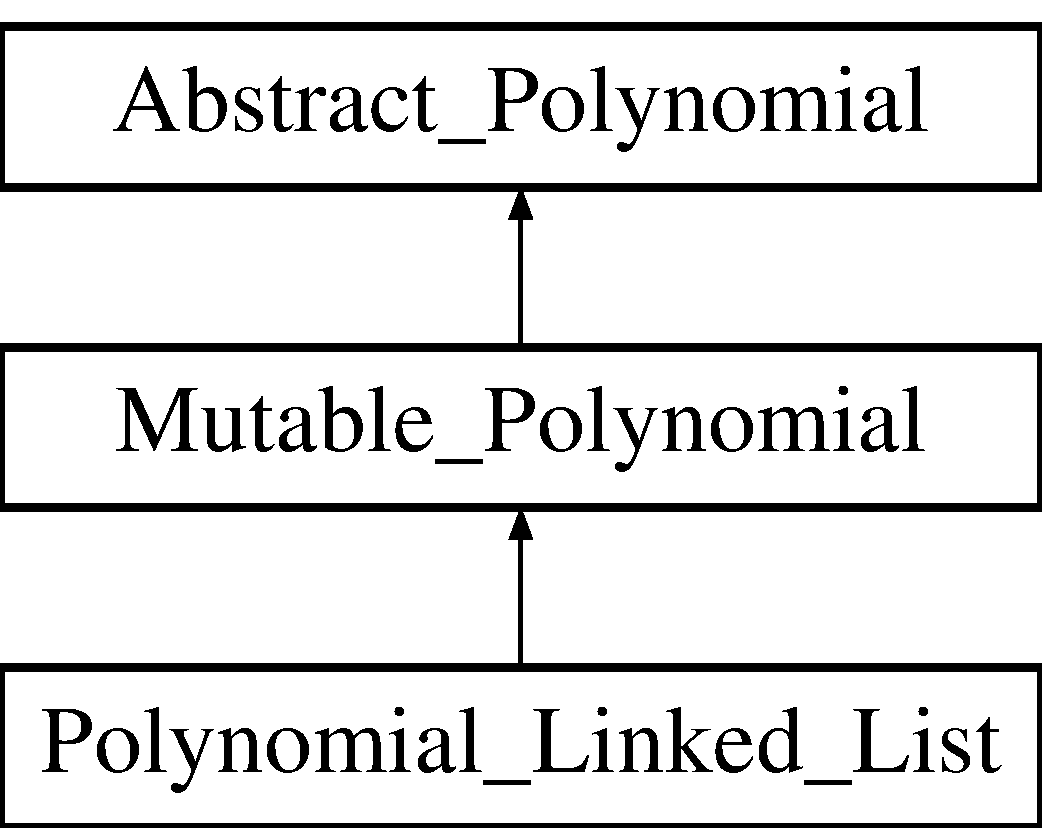
\includegraphics[height=2.000000cm]{group__polygroup}
\end{center}
\end{figure}
\index{Monomial\+\_\+\+Node@{Monomial\+\_\+\+Node}}\label{class_monomial___node}
\Hypertarget{group__polygroup_class_monomial___node}
\subsubsection{class Monomial\+\_\+\+Node}
Tool for \hyperlink{group__polygroup_class_polynomial___linked___list}{Polynomial\+\_\+\+Linked\+\_\+\+List}. 

\begin{DoxyAuthor}{Author}
John Perry 
\end{DoxyAuthor}
\begin{DoxyDate}{Date}
2015
\end{DoxyDate}
Each node in a linked list polynomial contains both the coefficient and the monomial. 

Definition at line 42 of file polynomial\+\_\+linked\+\_\+list.\+hpp.

\subsubsection*{Public Member Functions}
\begin{Indent}\textbf{ Construction}\par
\begin{DoxyCompactItemize}
\item 
\mbox{\Hypertarget{group__polygroup_af979446eca6482aa603a53681a0c1ce9}\label{group__polygroup_af979446eca6482aa603a53681a0c1ce9}} 
\hyperlink{group__polygroup_af979446eca6482aa603a53681a0c1ce9}{Monomial\+\_\+\+Node} (const \hyperlink{group___fields_group_class_prime___field___element}{Prime\+\_\+\+Field\+\_\+\+Element} \&a, const \hyperlink{group__polygroup_class_monomial}{Monomial} \&u)
\begin{DoxyCompactList}\small\item\em \hyperlink{group__polygroup_class_monomial}{Monomial} u with coefficient a. Both are copied, and can be deleted. \end{DoxyCompactList}\item 
\mbox{\Hypertarget{group__polygroup_a4de7838dc51013c36fe23831249a8096}\label{group__polygroup_a4de7838dc51013c36fe23831249a8096}} 
\hyperlink{group__polygroup_a4de7838dc51013c36fe23831249a8096}{Monomial\+\_\+\+Node} (\hyperlink{group___fields_group_class_prime___field}{Prime\+\_\+\+Field} \&F, const \hyperlink{group__polygroup_class_monomial}{Monomial} \&u)
\begin{DoxyCompactList}\small\item\em \hyperlink{group__polygroup_class_monomial}{Monomial} u (copied) with coefficient 1. \end{DoxyCompactList}\end{DoxyCompactItemize}
\end{Indent}
\begin{Indent}\textbf{ Basic properties}\par
\begin{DoxyCompactItemize}
\item 
\mbox{\Hypertarget{group__polygroup_ae2de10486486a056aa860ae8f133c309}\label{group__polygroup_ae2de10486486a056aa860ae8f133c309}} 
\hyperlink{group__polygroup_class_monomial}{Monomial} \& \hyperlink{group__polygroup_ae2de10486486a056aa860ae8f133c309}{monomial} ()
\begin{DoxyCompactList}\small\item\em This term's monomial, or power product. The coefficient is not included. \end{DoxyCompactList}\item 
\mbox{\Hypertarget{group__polygroup_a9eaedcc01e0c081565981450d08379f4}\label{group__polygroup_a9eaedcc01e0c081565981450d08379f4}} 
\hyperlink{group___fields_group_class_prime___field___element}{Prime\+\_\+\+Field\+\_\+\+Element} \& \hyperlink{group__polygroup_a9eaedcc01e0c081565981450d08379f4}{coefficient} ()
\begin{DoxyCompactList}\small\item\em This term's coefficient. \end{DoxyCompactList}\end{DoxyCompactItemize}
\end{Indent}
\begin{Indent}\textbf{ Memory management}\par
\begin{DoxyCompactItemize}
\item 
\mbox{\Hypertarget{group__polygroup_a556f9f54dca0f5407ec03c2ee88bac4b}\label{group__polygroup_a556f9f54dca0f5407ec03c2ee88bac4b}} 
void $\ast$ \hyperlink{group__polygroup_a556f9f54dca0f5407ec03c2ee88bac4b}{operator new} (size\+\_\+t)
\begin{DoxyCompactList}\small\item\em requests memory form \hyperlink{group__polygroup_class_monomial___node}{Monomial\+\_\+\+Node}\textquotesingle{}s \hyperlink{group__memorygroup_class_grading___order___data___allocator}{Grading\+\_\+\+Order\+\_\+\+Data\+\_\+\+Allocator} \end{DoxyCompactList}\item 
\mbox{\Hypertarget{group__polygroup_ae954b3ac41cf1c05b64c9b7f3c3d84a5}\label{group__polygroup_ae954b3ac41cf1c05b64c9b7f3c3d84a5}} 
void \hyperlink{group__polygroup_ae954b3ac41cf1c05b64c9b7f3c3d84a5}{operator delete} (void $\ast$)
\begin{DoxyCompactList}\small\item\em returns data to \hyperlink{group__polygroup_class_monomial___node}{Monomial\+\_\+\+Node}\textquotesingle{}s \hyperlink{group__memorygroup_class_grading___order___data___allocator}{Grading\+\_\+\+Order\+\_\+\+Data\+\_\+\+Allocator} \end{DoxyCompactList}\end{DoxyCompactItemize}
\end{Indent}
\subsubsection*{Protected Attributes}
\begin{DoxyCompactItemize}
\item 
\mbox{\Hypertarget{group__polygroup_aa1dcb82900a21ba573517b727a84dd27}\label{group__polygroup_aa1dcb82900a21ba573517b727a84dd27}} 
\hyperlink{group___fields_group_class_prime___field___element}{Prime\+\_\+\+Field\+\_\+\+Element} \hyperlink{group__polygroup_aa1dcb82900a21ba573517b727a84dd27}{c}
\begin{DoxyCompactList}\small\item\em the monomial's coefficient \end{DoxyCompactList}\item 
\mbox{\Hypertarget{group__polygroup_a21f0bb73c29eb42438c6ecc0262947bf}\label{group__polygroup_a21f0bb73c29eb42438c6ecc0262947bf}} 
\hyperlink{group__polygroup_class_monomial___node}{Monomial\+\_\+\+Node} $\ast$ \hyperlink{group__polygroup_a21f0bb73c29eb42438c6ecc0262947bf}{next}
\begin{DoxyCompactList}\small\item\em for linking \end{DoxyCompactList}\item 
\mbox{\Hypertarget{group__polygroup_a7f2913a95e35d7c0e7d8fd04968f9ed1}\label{group__polygroup_a7f2913a95e35d7c0e7d8fd04968f9ed1}} 
\hyperlink{group__polygroup_class_monomial___node}{Monomial\+\_\+\+Node} $\ast$ \hyperlink{group__polygroup_a7f2913a95e35d7c0e7d8fd04968f9ed1}{prev}
\begin{DoxyCompactList}\small\item\em for linking \end{DoxyCompactList}\item 
\mbox{\Hypertarget{group__polygroup_af30c51160297f65bb77d063e8e0ecaa6}\label{group__polygroup_af30c51160297f65bb77d063e8e0ecaa6}} 
\hyperlink{group__polygroup_class_monomial}{Monomial} \hyperlink{group__polygroup_af30c51160297f65bb77d063e8e0ecaa6}{t}
\begin{DoxyCompactList}\small\item\em the monomial in this node \end{DoxyCompactList}\end{DoxyCompactItemize}
\subsubsection*{Friends}
\begin{Indent}\textbf{ Iteration}\par
\begin{DoxyCompactItemize}
\item 
\mbox{\Hypertarget{group__polygroup_adc04ceaa684cbc36bd6800c57364bd2e}\label{group__polygroup_adc04ceaa684cbc36bd6800c57364bd2e}} 
class {\bfseries L\+L\+Polynomial\+\_\+\+Iterator}
\item 
\mbox{\Hypertarget{group__polygroup_a7e28ea806491074003c51b4d857abd6c}\label{group__polygroup_a7e28ea806491074003c51b4d857abd6c}} 
class {\bfseries Polynomial\+\_\+\+Linked\+\_\+\+List}
\end{DoxyCompactItemize}
\end{Indent}
\index{Mutable\+\_\+\+Polynomial@{Mutable\+\_\+\+Polynomial}}\label{class_mutable___polynomial}
\Hypertarget{group__polygroup_class_mutable___polynomial}
\subsubsection{class Mutable\+\_\+\+Polynomial}
Polynomials that need arithmetic typically descend from this class. 

\begin{DoxyAuthor}{Author}
John Perry 
\end{DoxyAuthor}
\begin{DoxyDate}{Date}
2015
\end{DoxyDate}
This class extends \hyperlink{group__polygroup_class_abstract___polynomial}{Abstract\+\_\+\+Polynomial} to allow for basic arithmetic of a polynomial. 

Definition at line 313 of file polynomial.\+hpp.

Inheritance diagram for Mutable\+\_\+\+Polynomial\+:\begin{figure}[H]
\begin{center}
\leavevmode
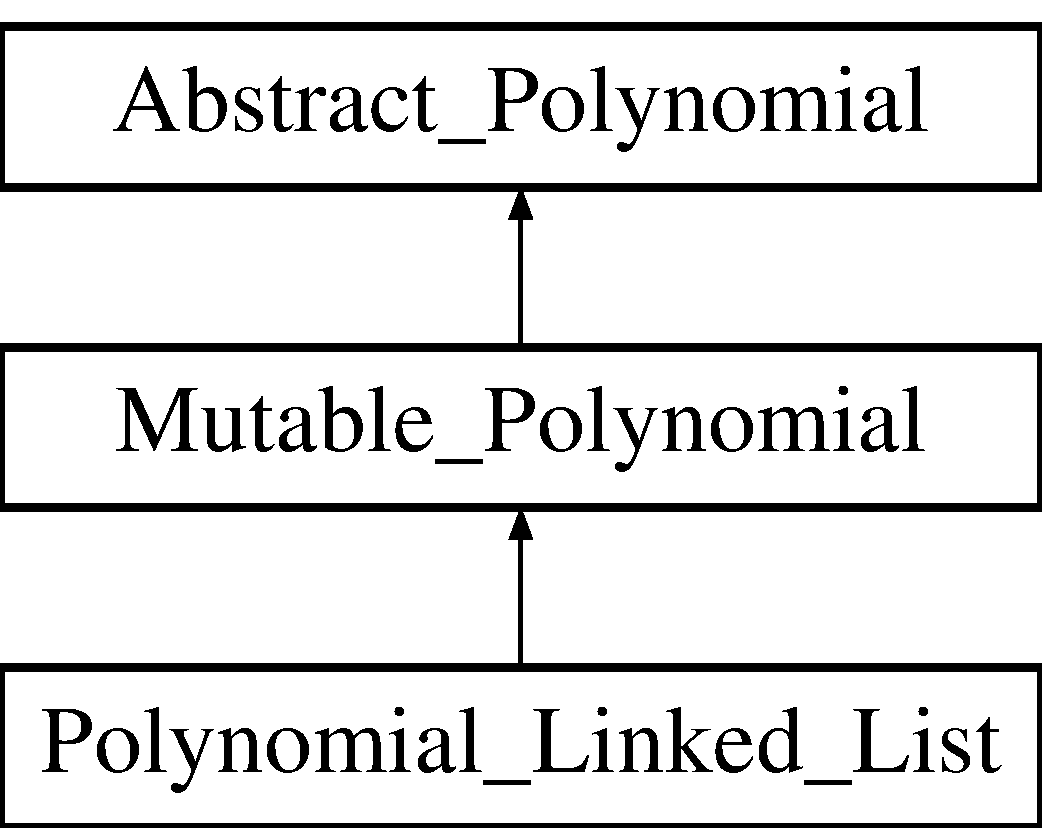
\includegraphics[height=3.000000cm]{group__polygroup}
\end{center}
\end{figure}
\subsubsection*{Public Member Functions}
\begin{Indent}\textbf{ Construction}\par
\begin{DoxyCompactItemize}
\item 
\mbox{\Hypertarget{group__polygroup_ad517faca8bbd385411603bbb20f29735}\label{group__polygroup_ad517faca8bbd385411603bbb20f29735}} 
\hyperlink{group__polygroup_ad517faca8bbd385411603bbb20f29735}{Mutable\+\_\+\+Polynomial} (\hyperlink{group__polygroup_class_polynomial___ring}{Polynomial\+\_\+\+Ring} \&\hyperlink{group__polygroup_a551ade20b7dcd96c227dd0401f6ffbbe}{R}, const \hyperlink{group__orderinggroup_class_monomial___ordering}{Monomial\+\_\+\+Ordering} $\ast$ordering=generic\+\_\+grevlex\+\_\+ptr)
\begin{DoxyCompactList}\small\item\em constructor \end{DoxyCompactList}\end{DoxyCompactItemize}
\end{Indent}
\begin{Indent}\textbf{ Destruction}\par
\begin{DoxyCompactItemize}
\item 
\mbox{\Hypertarget{group__polygroup_ad81cb5bb2a87a289c73fb6cd39afa029}\label{group__polygroup_ad81cb5bb2a87a289c73fb6cd39afa029}} 
virtual \hyperlink{group__polygroup_ad81cb5bb2a87a289c73fb6cd39afa029}{$\sim$\+Mutable\+\_\+\+Polynomial} ()=0
\begin{DoxyCompactList}\small\item\em destructor \end{DoxyCompactList}\end{DoxyCompactItemize}
\end{Indent}
\begin{Indent}\textbf{ Computation}\par
\begin{DoxyCompactItemize}
\item 
\mbox{\Hypertarget{group__polygroup_aa7a14a4cbb110840e55d656d7c6fe3ff}\label{group__polygroup_aa7a14a4cbb110840e55d656d7c6fe3ff}} 
virtual \hyperlink{group__polygroup_class_mutable___polynomial}{Mutable\+\_\+\+Polynomial} $\ast$ \hyperlink{group__polygroup_aa7a14a4cbb110840e55d656d7c6fe3ff}{zero\+\_\+polynomial} () const =0
\begin{DoxyCompactList}\small\item\em zero polynomial of this type \end{DoxyCompactList}\item 
\mbox{\Hypertarget{group__polygroup_a4d581c9c777591ab2cfdb3b4139c21da}\label{group__polygroup_a4d581c9c777591ab2cfdb3b4139c21da}} 
virtual \hyperlink{group__polygroup_class_mutable___polynomial}{Mutable\+\_\+\+Polynomial} \& \hyperlink{group__polygroup_a4d581c9c777591ab2cfdb3b4139c21da}{operator+=} (const \hyperlink{group__polygroup_class_abstract___polynomial}{Abstract\+\_\+\+Polynomial} \&)=0
\begin{DoxyCompactList}\small\item\em add another polynomial \end{DoxyCompactList}\item 
\mbox{\Hypertarget{group__polygroup_a6582d3b7af8a58f9645aac72fec01614}\label{group__polygroup_a6582d3b7af8a58f9645aac72fec01614}} 
virtual \hyperlink{group__polygroup_class_mutable___polynomial}{Mutable\+\_\+\+Polynomial} \& \hyperlink{group__polygroup_a6582d3b7af8a58f9645aac72fec01614}{operator-\/=} (const \hyperlink{group__polygroup_class_abstract___polynomial}{Abstract\+\_\+\+Polynomial} \&)=0
\begin{DoxyCompactList}\small\item\em subtract another polynomial \end{DoxyCompactList}\item 
\mbox{\Hypertarget{group__polygroup_add21309f55af6a58e1d9b1623a0bb09a}\label{group__polygroup_add21309f55af6a58e1d9b1623a0bb09a}} 
virtual void \hyperlink{group__polygroup_add21309f55af6a58e1d9b1623a0bb09a}{add\+\_\+polynomial\+\_\+multiple} (const \hyperlink{group___fields_group_class_prime___field___element}{Prime\+\_\+\+Field\+\_\+\+Element} \&, const \hyperlink{group__polygroup_class_monomial}{Monomial} \&, const \hyperlink{group__polygroup_class_abstract___polynomial}{Abstract\+\_\+\+Polynomial} \&, bool subtract=false)=0
\begin{DoxyCompactList}\small\item\em add monomial multiple of other \end{DoxyCompactList}\item 
\mbox{\Hypertarget{group__polygroup_a19f2326427ab08d6dc160c5eca898529}\label{group__polygroup_a19f2326427ab08d6dc160c5eca898529}} 
virtual void \hyperlink{group__polygroup_a19f2326427ab08d6dc160c5eca898529}{multiply\+\_\+by\+\_\+scalar} (const \hyperlink{group___fields_group_class_prime___field___element}{Prime\+\_\+\+Field\+\_\+\+Element} \&a)
\begin{DoxyCompactList}\small\item\em multiply by scalar \end{DoxyCompactList}\item 
\mbox{\Hypertarget{group__polygroup_a97a3ca070811ac495e8f22c3d7623225}\label{group__polygroup_a97a3ca070811ac495e8f22c3d7623225}} 
virtual void \hyperlink{group__polygroup_a97a3ca070811ac495e8f22c3d7623225}{multiply\+\_\+by\+\_\+monomial} (const \hyperlink{group__polygroup_class_monomial}{Monomial} \&t)
\begin{DoxyCompactList}\small\item\em multiply by monomial \end{DoxyCompactList}\item 
\mbox{\Hypertarget{group__polygroup_a0f40d2041aa5c3447324bde0c14049e2}\label{group__polygroup_a0f40d2041aa5c3447324bde0c14049e2}} 
virtual void \hyperlink{group__polygroup_a0f40d2041aa5c3447324bde0c14049e2}{reduce\+\_\+by} (const \hyperlink{group__polygroup_class_abstract___polynomial}{Abstract\+\_\+\+Polynomial} \&p)
\begin{DoxyCompactList}\small\item\em reduce by $p$ until no further reduction possible \end{DoxyCompactList}\item 
\mbox{\Hypertarget{group__polygroup_a828c980c211687bcf752ed0562a1961e}\label{group__polygroup_a828c980c211687bcf752ed0562a1961e}} 
virtual \hyperlink{group__polygroup_class_mutable___polynomial}{Mutable\+\_\+\+Polynomial} $\ast$ \hyperlink{group__polygroup_a828c980c211687bcf752ed0562a1961e}{monomial\+\_\+multiple} (const \hyperlink{group__polygroup_class_monomial}{Monomial} \&) const =0
\begin{DoxyCompactList}\small\item\em multiple of this and u \end{DoxyCompactList}\item 
\mbox{\Hypertarget{group__polygroup_a48d28e7a5fc543e18511f2dd24739ad7}\label{group__polygroup_a48d28e7a5fc543e18511f2dd24739ad7}} 
virtual \hyperlink{group__polygroup_class_mutable___polynomial}{Mutable\+\_\+\+Polynomial} $\ast$ \hyperlink{group__polygroup_a48d28e7a5fc543e18511f2dd24739ad7}{scalar\+\_\+multiple} (const \hyperlink{group___fields_group_class_prime___field___element}{Prime\+\_\+\+Field\+\_\+\+Element} \&) const =0
\begin{DoxyCompactList}\small\item\em multiple of this and c \end{DoxyCompactList}\end{DoxyCompactItemize}
\end{Indent}
\begin{Indent}\textbf{ Iteration}\par
\begin{DoxyCompactItemize}
\item 
\mbox{\Hypertarget{group__polygroup_a803892196221e618214c80987cec191a}\label{group__polygroup_a803892196221e618214c80987cec191a}} 
virtual \hyperlink{group___iterator_group_class_mutable___polynomial___iterator}{Mutable\+\_\+\+Polynomial\+\_\+\+Iterator} $\ast$ \hyperlink{group__polygroup_a803892196221e618214c80987cec191a}{new\+\_\+mutable\+\_\+iterator} ()=0
\begin{DoxyCompactList}\small\item\em An iterator that may modify the current position. \end{DoxyCompactList}\end{DoxyCompactItemize}
\end{Indent}
\begin{Indent}\textbf{ Modification}\par
\begin{DoxyCompactItemize}
\item 
\mbox{\Hypertarget{group__polygroup_a3acd7e39f907f95ab05a9ee68af7556c}\label{group__polygroup_a3acd7e39f907f95ab05a9ee68af7556c}} 
virtual \hyperlink{group__polygroup_class_mutable___polynomial}{Mutable\+\_\+\+Polynomial} $\ast$ \hyperlink{group__polygroup_a3acd7e39f907f95ab05a9ee68af7556c}{detach\+\_\+head} ()=0
\begin{DoxyCompactList}\small\item\em Remove and return the head. \end{DoxyCompactList}\item 
\mbox{\Hypertarget{group__polygroup_a966bd6c897acf04ac697bc0a4ca46a89}\label{group__polygroup_a966bd6c897acf04ac697bc0a4ca46a89}} 
virtual void \hyperlink{group__polygroup_a966bd6c897acf04ac697bc0a4ca46a89}{add\+\_\+last} (const \hyperlink{group___fields_group_class_prime___field___element}{Prime\+\_\+\+Field\+\_\+\+Element} \&, const \hyperlink{group__polygroup_class_monomial}{Monomial} \&)=0
\begin{DoxyCompactList}\small\item\em Attach a new monomial to the tail -- check that it belongs at tail! \end{DoxyCompactList}\end{DoxyCompactItemize}
\end{Indent}
\subsection*{Additional Inherited Members}
\index{Polynomial\+\_\+\+Geobucket@{Polynomial\+\_\+\+Geobucket}}\label{class_polynomial___geobucket}
\Hypertarget{group__polygroup_class_polynomial___geobucket}
\subsubsection{class Polynomial\+\_\+\+Geobucket}
Implementation of geobuckets. 

\begin{DoxyAuthor}{Author}
John Perry 
\end{DoxyAuthor}
\begin{DoxyDate}{Date}
2015 
\end{DoxyDate}
\begin{DoxyWarning}{Warning}
After any operation that might modify the leading term (such as adding, subtracting polynomials -- {\itshape not,} however, scalar or monomial multiplication) you will need to call \hyperlink{group__polygroup_ab57dbe8d5f0d3860997775d9f354ab0c}{recompute\+\_\+leading\+\_\+monomial()}. 

Exceeding the number of buckets will raise an exception. This will occur when a partial sum's size exceeds {\ttfamily N\+U\+M\+\_\+\+B\+U\+C\+K\+E\+TS}. 
\end{DoxyWarning}


Definition at line 114 of file polynomial\+\_\+geobucket.\+hpp.

Inheritance diagram for Polynomial\+\_\+\+Geobucket\+:\begin{figure}[H]
\begin{center}
\leavevmode
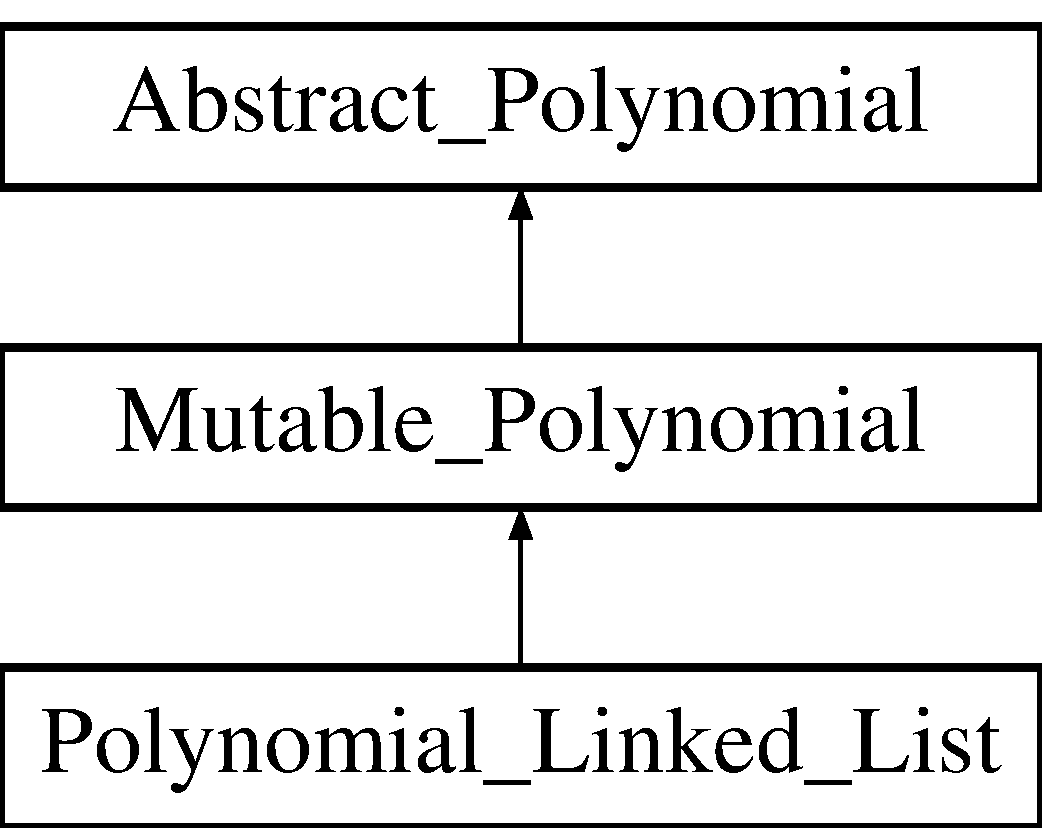
\includegraphics[height=3.000000cm]{group__polygroup}
\end{center}
\end{figure}
\subsubsection*{Public Member Functions}
\begin{Indent}\textbf{ Construction}\par
\begin{DoxyCompactItemize}
\item 
\mbox{\Hypertarget{group__polygroup_a1ddbd2520d7fa5b27ef27c66833fe074}\label{group__polygroup_a1ddbd2520d7fa5b27ef27c66833fe074}} 
\hyperlink{group__polygroup_a1ddbd2520d7fa5b27ef27c66833fe074}{Polynomial\+\_\+\+Geobucket} (\hyperlink{group__polygroup_class_polynomial___ring}{Polynomial\+\_\+\+Ring} \&\hyperlink{group__polygroup_a551ade20b7dcd96c227dd0401f6ffbbe}{R}, \hyperlink{group__orderinggroup_class_monomial___ordering}{Monomial\+\_\+\+Ordering} $\ast$order=generic\+\_\+grevlex\+\_\+ptr)
\begin{DoxyCompactList}\small\item\em Initializes a polynomial with the given number of variables, over the given field. \end{DoxyCompactList}\item 
\mbox{\Hypertarget{group__polygroup_a220910eae57ee32ec35a56344e3297b6}\label{group__polygroup_a220910eae57ee32ec35a56344e3297b6}} 
\hyperlink{group__polygroup_a220910eae57ee32ec35a56344e3297b6}{Polynomial\+\_\+\+Geobucket} (\hyperlink{group__polygroup_class_abstract___polynomial}{Abstract\+\_\+\+Polynomial} \&p)
\begin{DoxyCompactList}\small\item\em Initializes a geobucket that is a copy of $p$. \end{DoxyCompactList}\end{DoxyCompactItemize}
\end{Indent}
\begin{Indent}\textbf{ Destruction}\par
\begin{DoxyCompactItemize}
\item 
\mbox{\Hypertarget{group__polygroup_aa943e78f99a7e6d61ed5d962f05d34b1}\label{group__polygroup_aa943e78f99a7e6d61ed5d962f05d34b1}} 
\hyperlink{group__polygroup_aa943e78f99a7e6d61ed5d962f05d34b1}{$\sim$\+Polynomial\+\_\+\+Geobucket} ()
\begin{DoxyCompactList}\small\item\em Deallocates buckets, if they exist. \end{DoxyCompactList}\end{DoxyCompactItemize}
\end{Indent}
\begin{Indent}\textbf{ Basic properties}\par
\begin{DoxyCompactItemize}
\item 
virtual void \hyperlink{group__polygroup_ad3c705cb5c03be2ed62fea65101d1195}{sort\+\_\+by\+\_\+order} () override
\begin{DoxyCompactList}\small\item\em sorts each geobucket \end{DoxyCompactList}\item 
virtual void \hyperlink{group__polygroup_ad3298b3201f53d0ddaa657206c140ca8}{set\+\_\+monomial\+\_\+ordering} (const \hyperlink{group__orderinggroup_class_monomial___ordering}{Monomial\+\_\+\+Ordering} $\ast$order, bool sort\+\_\+anew=true) override
\begin{DoxyCompactList}\small\item\em sets the monomial ordering for each bucket \end{DoxyCompactList}\item 
virtual \hyperlink{group__polygroup_class_monomial}{Monomial} \& \hyperlink{group__polygroup_aeb9d72c577af4de04e1e4cce04a9f41f}{leading\+\_\+monomial} () const override
\begin{DoxyCompactList}\small\item\em returns the leading monomial \end{DoxyCompactList}\item 
virtual \hyperlink{group___fields_group_class_prime___field___element}{Prime\+\_\+\+Field\+\_\+\+Element} \hyperlink{group__polygroup_a096aa08d1d7be3522c140908989e4dea}{leading\+\_\+coefficient} () const override
\begin{DoxyCompactList}\small\item\em returns the leading coefficient \end{DoxyCompactList}\item 
virtual unsigned \hyperlink{group__polygroup_a691f704d695210841a60fe2e6791d1af}{length} () const override
\begin{DoxyCompactList}\small\item\em how long is this polynomial? \end{DoxyCompactList}\item 
virtual \hyperlink{group__polygroup_class_polynomial___linked___list}{Polynomial\+\_\+\+Linked\+\_\+\+List} $\ast$ \hyperlink{group__polygroup_a7723d297ad268bb7139b1592f4e2eaff}{zero\+\_\+polynomial} () const override
\begin{DoxyCompactList}\small\item\em creates and returns a geobucket initialized to zero \end{DoxyCompactList}\item 
virtual bool \hyperlink{group__polygroup_ac71d7f640ebdf764c5b81bf8d9a5686d}{is\+\_\+zero} () const override
\begin{DoxyCompactList}\small\item\em is this polynomial zero? \end{DoxyCompactList}\item 
\mbox{\Hypertarget{group__polygroup_af6fc5e1931972bd9e5f296ca719a1815}\label{group__polygroup_af6fc5e1931972bd9e5f296ca719a1815}} 
virtual bool \hyperlink{group__polygroup_af6fc5e1931972bd9e5f296ca719a1815}{can\+\_\+reduce} (\hyperlink{group__polygroup_class_abstract___polynomial}{Abstract\+\_\+\+Polynomial} \&other) const override
\begin{DoxyCompactList}\small\item\em Whether {\ttfamily this} can reduce {\ttfamily other}. A geobucket should not generally be used to reduce other polynomials, so avoid this like the plague. \end{DoxyCompactList}\item 
\mbox{\Hypertarget{group__polygroup_a08a6bd3fd143c05e1b2762a7f239b371}\label{group__polygroup_a08a6bd3fd143c05e1b2762a7f239b371}} 
virtual \hyperlink{group___iterator_group_class_geobucket___iterator}{Geobucket\+\_\+\+Iterator} $\ast$ \hyperlink{group__polygroup_a08a6bd3fd143c05e1b2762a7f239b371}{new\+\_\+iterator} () const override
\begin{DoxyCompactList}\small\item\em An iterator that poses no risk of modifying the polynomial. \end{DoxyCompactList}\item 
\mbox{\Hypertarget{group__polygroup_a0c5f05f041e6d2c462d1dcb2bdd39df0}\label{group__polygroup_a0c5f05f041e6d2c462d1dcb2bdd39df0}} 
virtual \hyperlink{group___iterator_group_class_polynomial___iterator}{Polynomial\+\_\+\+Iterator} $\ast$ \hyperlink{group__polygroup_a0c5f05f041e6d2c462d1dcb2bdd39df0}{begin} () const override
\begin{DoxyCompactList}\small\item\em returns an iterator to the polynomial's leading monomial \end{DoxyCompactList}\item 
\mbox{\Hypertarget{group__polygroup_a28dde5c7941ad0636f17054cd80bbd8e}\label{group__polygroup_a28dde5c7941ad0636f17054cd80bbd8e}} 
virtual \hyperlink{group___iterator_group_class_polynomial___iterator}{Polynomial\+\_\+\+Iterator} $\ast$ \hyperlink{group__polygroup_a28dde5c7941ad0636f17054cd80bbd8e}{end} () const override
\begin{DoxyCompactList}\small\item\em iterator to last monomial \end{DoxyCompactList}\item 
\mbox{\Hypertarget{group__polygroup_a630c245914a9235dd84af2b34deb778d}\label{group__polygroup_a630c245914a9235dd84af2b34deb778d}} 
virtual \hyperlink{group___iterator_group_class_geobucket___iterator}{Geobucket\+\_\+\+Iterator} $\ast$ \hyperlink{group__polygroup_a630c245914a9235dd84af2b34deb778d}{new\+\_\+mutable\+\_\+iterator} () override
\begin{DoxyCompactList}\small\item\em An iterator that may modify the current position. \end{DoxyCompactList}\end{DoxyCompactItemize}
\end{Indent}
\begin{Indent}\textbf{ Computation}\par
\begin{DoxyCompactItemize}
\item 
void \hyperlink{group__polygroup_ab57dbe8d5f0d3860997775d9f354ab0c}{recompute\+\_\+leading\+\_\+monomial} ()
\begin{DoxyCompactList}\small\item\em You will need to call this after every operation that might modify the leading term. \end{DoxyCompactList}\item 
\mbox{\Hypertarget{group__polygroup_a2f474c58fa933e4183b1a165ef3b814d}\label{group__polygroup_a2f474c58fa933e4183b1a165ef3b814d}} 
virtual \hyperlink{group__polygroup_class_polynomial___geobucket}{Polynomial\+\_\+\+Geobucket} $\ast$ \hyperlink{group__polygroup_a2f474c58fa933e4183b1a165ef3b814d}{monomial\+\_\+multiple} (const \hyperlink{group__polygroup_class_monomial}{Monomial} \&t) const override
\begin{DoxyCompactList}\small\item\em Returns $\texttt{this}\times t$. \end{DoxyCompactList}\item 
\mbox{\Hypertarget{group__polygroup_a0a62c427fc0d8cffce4a875597ab3cc0}\label{group__polygroup_a0a62c427fc0d8cffce4a875597ab3cc0}} 
virtual \hyperlink{group__polygroup_class_polynomial___geobucket}{Polynomial\+\_\+\+Geobucket} $\ast$ \hyperlink{group__polygroup_a0a62c427fc0d8cffce4a875597ab3cc0}{scalar\+\_\+multiple} (const \hyperlink{group___fields_group_class_prime___field___element}{Prime\+\_\+\+Field\+\_\+\+Element} \&a) const override
\begin{DoxyCompactList}\small\item\em Returns $\texttt{this}\times a$. \end{DoxyCompactList}\item 
\mbox{\Hypertarget{group__polygroup_a93d4a23dc1e7d76b26bfc1b9d544ed07}\label{group__polygroup_a93d4a23dc1e7d76b26bfc1b9d544ed07}} 
virtual \hyperlink{group__polygroup_class_polynomial___geobucket}{Polynomial\+\_\+\+Geobucket} \& \hyperlink{group__polygroup_a93d4a23dc1e7d76b26bfc1b9d544ed07}{operator+=} (const \hyperlink{group__polygroup_class_abstract___polynomial}{Abstract\+\_\+\+Polynomial} \&g) override
\begin{DoxyCompactList}\small\item\em Adds $g$ to {\ttfamily this}. Recomputes leading monomial. \end{DoxyCompactList}\item 
\mbox{\Hypertarget{group__polygroup_adceeadff156d68eb4af0492d5cbd46b5}\label{group__polygroup_adceeadff156d68eb4af0492d5cbd46b5}} 
virtual \hyperlink{group__polygroup_class_polynomial___geobucket}{Polynomial\+\_\+\+Geobucket} \& \hyperlink{group__polygroup_adceeadff156d68eb4af0492d5cbd46b5}{operator-\/=} (const \hyperlink{group__polygroup_class_abstract___polynomial}{Abstract\+\_\+\+Polynomial} \&g) override
\begin{DoxyCompactList}\small\item\em Subtracts $g$ from {\ttfamily this}. Recomputes leading monomial. \end{DoxyCompactList}\item 
\mbox{\Hypertarget{group__polygroup_a69a7a060044c2cb3aa32ba5c321a9eb4}\label{group__polygroup_a69a7a060044c2cb3aa32ba5c321a9eb4}} 
virtual void \hyperlink{group__polygroup_a69a7a060044c2cb3aa32ba5c321a9eb4}{add\+\_\+polynomial\+\_\+multiple} (const \hyperlink{group___fields_group_class_prime___field___element}{Prime\+\_\+\+Field\+\_\+\+Element} \&b, const \hyperlink{group__polygroup_class_monomial}{Monomial} \&u, const \hyperlink{group__polygroup_class_abstract___polynomial}{Abstract\+\_\+\+Polynomial} \&g, bool subtract=false) override
\begin{DoxyCompactList}\small\item\em Adds $bug$ to {\ttfamily this}. Recomputes leading monomial. \end{DoxyCompactList}\item 
\mbox{\Hypertarget{group__polygroup_a57606623bed3fcd4f7b38530af211346}\label{group__polygroup_a57606623bed3fcd4f7b38530af211346}} 
virtual \hyperlink{group__polygroup_class_polynomial___linked___list}{Polynomial\+\_\+\+Linked\+\_\+\+List} $\ast$ \hyperlink{group__polygroup_a57606623bed3fcd4f7b38530af211346}{detach\+\_\+head} () override
\begin{DoxyCompactList}\small\item\em Detaches the head and recomputes leading monomial. \end{DoxyCompactList}\item 
virtual void \hyperlink{group__polygroup_ada4a539d3666cd6801a75c8861bc35fa}{add\+\_\+last} (const \hyperlink{group___fields_group_class_prime___field___element}{Prime\+\_\+\+Field\+\_\+\+Element} \&a, const \hyperlink{group__polygroup_class_monomial}{Monomial} \&t) override
\begin{DoxyCompactList}\small\item\em Adds $at$ as a monomial of {\ttfamily this}. (Not necessarily the last!) \end{DoxyCompactList}\item 
\hyperlink{group__polygroup_class_abstract___polynomial}{Abstract\+\_\+\+Polynomial} $\ast$ \hyperlink{group__polygroup_aa76d2c0dce16690b01e8a8c4862b11c5}{canonicalize} (bool constant\+\_\+result=false)
\begin{DoxyCompactList}\small\item\em returns a copy of {\ttfamily this} in a simplified linear form \end{DoxyCompactList}\end{DoxyCompactItemize}
\end{Indent}
\subsubsection*{Protected Member Functions}
\begin{DoxyCompactItemize}
\item 
unsigned \hyperlink{group__polygroup_a82e8a9286f5c30e48c13e05d74af7fb9}{lglen} (unsigned i)
\begin{DoxyCompactList}\small\item\em Log-\/length of $i$, used to select a bucket for a polynomial of length $i$. \end{DoxyCompactList}\end{DoxyCompactItemize}
\subsubsection*{Protected Attributes}
\begin{DoxyCompactItemize}
\item 
\mbox{\Hypertarget{group__polygroup_abfbb6cf257943fb08e03ea4601cf3134}\label{group__polygroup_abfbb6cf257943fb08e03ea4601cf3134}} 
\hyperlink{group__polygroup_class_polynomial___linked___list}{Polynomial\+\_\+\+Linked\+\_\+\+List} $\ast$$\ast$ \hyperlink{group__polygroup_abfbb6cf257943fb08e03ea4601cf3134}{buckets}
\begin{DoxyCompactList}\small\item\em Array of ptrs to linked list polys; most initialized to {\ttfamily nullptr}. \end{DoxyCompactList}\end{DoxyCompactItemize}
\subsubsection*{Friends}
\begin{DoxyCompactItemize}
\item 
\mbox{\Hypertarget{group__polygroup_a45580077827a8fdbd6d2fabdbb2a2d7f}\label{group__polygroup_a45580077827a8fdbd6d2fabdbb2a2d7f}} 
class \hyperlink{group__polygroup_a45580077827a8fdbd6d2fabdbb2a2d7f}{Geobucket\+\_\+\+Iterator}
\begin{DoxyCompactList}\small\item\em to iterate over {\ttfamily this} and possibly change it \end{DoxyCompactList}\end{DoxyCompactItemize}
\subsubsection*{I/O}
\begin{DoxyCompactItemize}
\item 
ostream \& \hyperlink{group__polygroup_af97062198c6ade3e8d3077308e89669d}{operator$<$$<$} (ostream \&, const \hyperlink{group__polygroup_class_polynomial___geobucket}{Polynomial\+\_\+\+Geobucket} \&)
\begin{DoxyCompactList}\small\item\em prints the geobucket in an explicitly geobucket form \end{DoxyCompactList}\item 
void \hyperlink{group__polygroup_a672dd35e16935aaa5d5334283eab918e}{print} (unsigned i, ostream \&os=cout) const
\begin{DoxyCompactList}\small\item\em prints the $i$th bucket \end{DoxyCompactList}\item 
virtual void \hyperlink{group__polygroup_a3c8cb0c53e9acf4d60345fb4b4dbb807}{print} (ostream \&os=cout) const override
\begin{DoxyCompactList}\small\item\em prints the polynomial with an explicitly bucket form \end{DoxyCompactList}\end{DoxyCompactItemize}


\paragraph{Member Function Documentation}
\mbox{\Hypertarget{group__polygroup_ada4a539d3666cd6801a75c8861bc35fa}\label{group__polygroup_ada4a539d3666cd6801a75c8861bc35fa}} 
\index{Polynomial\+\_\+\+Geobucket@{Polynomial\+\_\+\+Geobucket}!add\+\_\+last@{add\+\_\+last}}
\index{add\+\_\+last@{add\+\_\+last}!Polynomial\+\_\+\+Geobucket@{Polynomial\+\_\+\+Geobucket}}
\subparagraph{\texorpdfstring{add\+\_\+last()}{add\_last()}}
{\footnotesize\ttfamily void Polynomial\+\_\+\+Geobucket\+::add\+\_\+last (\begin{DoxyParamCaption}\item[{const \hyperlink{group___fields_group_class_prime___field___element}{Prime\+\_\+\+Field\+\_\+\+Element} \&}]{a,  }\item[{const \hyperlink{group__polygroup_class_monomial}{Monomial} \&}]{t }\end{DoxyParamCaption})\hspace{0.3cm}{\ttfamily [override]}, {\ttfamily [virtual]}}



Adds $at$ as a monomial of {\ttfamily this}. (Not necessarily the last!) 


\begin{DoxyParams}{Parameters}
{\em a} & coefficient of the term to add \\
\hline
{\em t} & \hyperlink{group__polygroup_class_monomial}{Monomial} of the term to add \\
\hline
\end{DoxyParams}
\begin{DoxyWarning}{Warning}
In the case of a geobucket, \hyperlink{group__polygroup_ada4a539d3666cd6801a75c8861bc35fa}{add\+\_\+last()} doesn't really make sense (the last monomial might not be in order, after all) so this should not be used. As in the usual case, we do assume it belongs at the tail; we simply add it to a tail bucket (i.\+e., not {\ttfamily bucket\mbox{[}0\mbox{]}}). 
\end{DoxyWarning}


Implements \hyperlink{group__polygroup_a966bd6c897acf04ac697bc0a4ca46a89}{Mutable\+\_\+\+Polynomial}.



Definition at line 363 of file polynomial\+\_\+geobucket.\+cpp.

\mbox{\Hypertarget{group__polygroup_aa76d2c0dce16690b01e8a8c4862b11c5}\label{group__polygroup_aa76d2c0dce16690b01e8a8c4862b11c5}} 
\index{Polynomial\+\_\+\+Geobucket@{Polynomial\+\_\+\+Geobucket}!canonicalize@{canonicalize}}
\index{canonicalize@{canonicalize}!Polynomial\+\_\+\+Geobucket@{Polynomial\+\_\+\+Geobucket}}
\subparagraph{\texorpdfstring{canonicalize()}{canonicalize()}}
{\footnotesize\ttfamily \hyperlink{group__polygroup_class_abstract___polynomial}{Abstract\+\_\+\+Polynomial} $\ast$ Polynomial\+\_\+\+Geobucket\+::canonicalize (\begin{DoxyParamCaption}\item[{bool}]{constant\+\_\+result = {\ttfamily false} }\end{DoxyParamCaption})}



returns a copy of {\ttfamily this} in a simplified linear form 


\begin{DoxyParams}{Parameters}
{\em constant\+\_\+result} & whether you want a \hyperlink{group__polygroup_class_constant___polynomial}{Constant\+\_\+\+Polynomial}\\
\hline
\end{DoxyParams}
If {\ttfamily constant\+\_\+result} is {\ttfamily true}, the result is a {\ttfamily \hyperlink{group__polygroup_class_constant___polynomial}{Constant\+\_\+\+Polynomial}}. Otherwise, the result is a {\ttfamily \hyperlink{group__polygroup_class_polynomial___linked___list}{Polynomial\+\_\+\+Linked\+\_\+\+List}}. Choose the latter if you anticipate further reduction, such as tail reduction. (Geobuckets by default do not reduce lower-\/order terms.) \begin{DoxyReturn}{Returns}
a copy of {\ttfamily this} in a simplified linear form 
\end{DoxyReturn}


Definition at line 378 of file polynomial\+\_\+geobucket.\+cpp.

\mbox{\Hypertarget{group__polygroup_ac71d7f640ebdf764c5b81bf8d9a5686d}\label{group__polygroup_ac71d7f640ebdf764c5b81bf8d9a5686d}} 
\index{Polynomial\+\_\+\+Geobucket@{Polynomial\+\_\+\+Geobucket}!is\+\_\+zero@{is\+\_\+zero}}
\index{is\+\_\+zero@{is\+\_\+zero}!Polynomial\+\_\+\+Geobucket@{Polynomial\+\_\+\+Geobucket}}
\subparagraph{\texorpdfstring{is\+\_\+zero()}{is\_zero()}}
{\footnotesize\ttfamily bool Polynomial\+\_\+\+Geobucket\+::is\+\_\+zero (\begin{DoxyParamCaption}{ }\end{DoxyParamCaption}) const\hspace{0.3cm}{\ttfamily [override]}, {\ttfamily [virtual]}}



is this polynomial zero? 

\begin{DoxyReturn}{Returns}
{\ttfamily true} iff all the buckets are {\ttfamily nullptr} or themselves zero 
\end{DoxyReturn}
\begin{DoxySeeAlso}{See also}
Fixed\+\_\+\+Length\+\_\+\+Polynomial 
\end{DoxySeeAlso}


Implements \hyperlink{group__polygroup_afb4895702dd56895a792850a831c2f51}{Abstract\+\_\+\+Polynomial}.



Definition at line 201 of file polynomial\+\_\+geobucket.\+cpp.

\mbox{\Hypertarget{group__polygroup_a096aa08d1d7be3522c140908989e4dea}\label{group__polygroup_a096aa08d1d7be3522c140908989e4dea}} 
\index{Polynomial\+\_\+\+Geobucket@{Polynomial\+\_\+\+Geobucket}!leading\+\_\+coefficient@{leading\+\_\+coefficient}}
\index{leading\+\_\+coefficient@{leading\+\_\+coefficient}!Polynomial\+\_\+\+Geobucket@{Polynomial\+\_\+\+Geobucket}}
\subparagraph{\texorpdfstring{leading\+\_\+coefficient()}{leading\_coefficient()}}
{\footnotesize\ttfamily \hyperlink{group___fields_group_class_prime___field___element}{Prime\+\_\+\+Field\+\_\+\+Element} Polynomial\+\_\+\+Geobucket\+::leading\+\_\+coefficient (\begin{DoxyParamCaption}{ }\end{DoxyParamCaption}) const\hspace{0.3cm}{\ttfamily [override]}, {\ttfamily [virtual]}}



returns the leading coefficient 

\begin{DoxyReturn}{Returns}
the leading coefficient 
\end{DoxyReturn}
\begin{DoxyWarning}{Warning}
Does not recompute the leading monomial first. Make sure the leading monomial exists and is valid. 

Descendants that perform any arithemtic that might change the leading monomial should invoke \hyperlink{group__polygroup_ab57dbe8d5f0d3860997775d9f354ab0c}{recompute\+\_\+leading\+\_\+monomial()} before this. The class's own functions for arithmetic do this automatically (or should). 
\end{DoxyWarning}


Implements \hyperlink{group__polygroup_a511ce8e997fe3fd1141293d256e25fad}{Abstract\+\_\+\+Polynomial}.



Definition at line 185 of file polynomial\+\_\+geobucket.\+cpp.

\mbox{\Hypertarget{group__polygroup_aeb9d72c577af4de04e1e4cce04a9f41f}\label{group__polygroup_aeb9d72c577af4de04e1e4cce04a9f41f}} 
\index{Polynomial\+\_\+\+Geobucket@{Polynomial\+\_\+\+Geobucket}!leading\+\_\+monomial@{leading\+\_\+monomial}}
\index{leading\+\_\+monomial@{leading\+\_\+monomial}!Polynomial\+\_\+\+Geobucket@{Polynomial\+\_\+\+Geobucket}}
\subparagraph{\texorpdfstring{leading\+\_\+monomial()}{leading\_monomial()}}
{\footnotesize\ttfamily \hyperlink{group__polygroup_class_monomial}{Monomial} \& Polynomial\+\_\+\+Geobucket\+::leading\+\_\+monomial (\begin{DoxyParamCaption}{ }\end{DoxyParamCaption}) const\hspace{0.3cm}{\ttfamily [override]}, {\ttfamily [virtual]}}



returns the leading monomial 

\begin{DoxyReturn}{Returns}
the leading monomial 
\end{DoxyReturn}
\begin{DoxyWarning}{Warning}
Does not recompute the leading monomial first. Make sure the leading monomial exists and is valid. 

Descendants that perform any arithemtic that might change the leading monomial should invoke \hyperlink{group__polygroup_ab57dbe8d5f0d3860997775d9f354ab0c}{recompute\+\_\+leading\+\_\+monomial()} before this. The class's own functions for arithmetic do this automatically (or should). 
\end{DoxyWarning}


Implements \hyperlink{group__polygroup_a9186ed0f55c5cc4ecb1b9bc11ba9f679}{Abstract\+\_\+\+Polynomial}.



Definition at line 181 of file polynomial\+\_\+geobucket.\+cpp.

\mbox{\Hypertarget{group__polygroup_a691f704d695210841a60fe2e6791d1af}\label{group__polygroup_a691f704d695210841a60fe2e6791d1af}} 
\index{Polynomial\+\_\+\+Geobucket@{Polynomial\+\_\+\+Geobucket}!length@{length}}
\index{length@{length}!Polynomial\+\_\+\+Geobucket@{Polynomial\+\_\+\+Geobucket}}
\subparagraph{\texorpdfstring{length()}{length()}}
{\footnotesize\ttfamily unsigned Polynomial\+\_\+\+Geobucket\+::length (\begin{DoxyParamCaption}{ }\end{DoxyParamCaption}) const\hspace{0.3cm}{\ttfamily [override]}, {\ttfamily [virtual]}}



how long is this polynomial? 

\begin{DoxyReturn}{Returns}
number of monomials in this polynomial 
\end{DoxyReturn}
\begin{DoxyWarning}{Warning}
This will not include potential simplification of monomials. A geobucket does not simplify non-\/leading terms until canonicalization. 
\end{DoxyWarning}


Implements \hyperlink{group__polygroup_a48f4c3c030ca66a9386cd71f71d5def7}{Abstract\+\_\+\+Polynomial}.



Definition at line 189 of file polynomial\+\_\+geobucket.\+cpp.

\mbox{\Hypertarget{group__polygroup_a82e8a9286f5c30e48c13e05d74af7fb9}\label{group__polygroup_a82e8a9286f5c30e48c13e05d74af7fb9}} 
\index{Polynomial\+\_\+\+Geobucket@{Polynomial\+\_\+\+Geobucket}!lglen@{lglen}}
\index{lglen@{lglen}!Polynomial\+\_\+\+Geobucket@{Polynomial\+\_\+\+Geobucket}}
\subparagraph{\texorpdfstring{lglen()}{lglen()}}
{\footnotesize\ttfamily unsigned Polynomial\+\_\+\+Geobucket\+::lglen (\begin{DoxyParamCaption}\item[{unsigned}]{i }\end{DoxyParamCaption})\hspace{0.3cm}{\ttfamily [inline]}, {\ttfamily [protected]}}



Log-\/length of $i$, used to select a bucket for a polynomial of length $i$. 


\begin{DoxyParams}{Parameters}
{\em i} & number of terms we need space for \\
\hline
\end{DoxyParams}
\begin{DoxyReturn}{Returns}
the smallest power of 2 larger than i 
\end{DoxyReturn}


Definition at line 302 of file polynomial\+\_\+geobucket.\+hpp.

\mbox{\Hypertarget{group__polygroup_a672dd35e16935aaa5d5334283eab918e}\label{group__polygroup_a672dd35e16935aaa5d5334283eab918e}} 
\index{Polynomial\+\_\+\+Geobucket@{Polynomial\+\_\+\+Geobucket}!print@{print}}
\index{print@{print}!Polynomial\+\_\+\+Geobucket@{Polynomial\+\_\+\+Geobucket}}
\subparagraph{\texorpdfstring{print()}{print()}\hspace{0.1cm}{\footnotesize\ttfamily [1/2]}}
{\footnotesize\ttfamily void Polynomial\+\_\+\+Geobucket\+::print (\begin{DoxyParamCaption}\item[{unsigned}]{i,  }\item[{ostream \&}]{os = {\ttfamily cout} }\end{DoxyParamCaption}) const}



prints the $i$th bucket 


\begin{DoxyParams}{Parameters}
{\em i} & which bucket to print \\
\hline
{\em os} & where to print the bucket\\
\hline
\end{DoxyParams}
In the context of geobuckets, this makes more sense than printing the polynomial. Practically, printing the polynomial does the same thing as printing the contents of the buckets, but the more general function can be misleading on account of the un-\/simplified nature of the polynomial. 

Definition at line 399 of file polynomial\+\_\+geobucket.\+cpp.

\mbox{\Hypertarget{group__polygroup_a3c8cb0c53e9acf4d60345fb4b4dbb807}\label{group__polygroup_a3c8cb0c53e9acf4d60345fb4b4dbb807}} 
\index{Polynomial\+\_\+\+Geobucket@{Polynomial\+\_\+\+Geobucket}!print@{print}}
\index{print@{print}!Polynomial\+\_\+\+Geobucket@{Polynomial\+\_\+\+Geobucket}}
\subparagraph{\texorpdfstring{print()}{print()}\hspace{0.1cm}{\footnotesize\ttfamily [2/2]}}
{\footnotesize\ttfamily void Polynomial\+\_\+\+Geobucket\+::print (\begin{DoxyParamCaption}\item[{ostream \&}]{os = {\ttfamily cout} }\end{DoxyParamCaption}) const\hspace{0.3cm}{\ttfamily [override]}, {\ttfamily [virtual]}}



prints the polynomial with an explicitly bucket form 


\begin{DoxyParams}{Parameters}
{\em os} & where to print the polynomial\\
\hline
\end{DoxyParams}
Prints the polynomial in the form \[(b_1) + (b_2) + \cdots + (b_\textrm{last}).\] Parentheses separate buckets, whose sums have not (yet) been simplified. Uninitiated and nonzero buckets are not printed. 

Reimplemented from \hyperlink{group__polygroup_adbbb6af1fb79d5794af42e28d584641b}{Abstract\+\_\+\+Polynomial}.



Definition at line 403 of file polynomial\+\_\+geobucket.\+cpp.

\mbox{\Hypertarget{group__polygroup_ab57dbe8d5f0d3860997775d9f354ab0c}\label{group__polygroup_ab57dbe8d5f0d3860997775d9f354ab0c}} 
\index{Polynomial\+\_\+\+Geobucket@{Polynomial\+\_\+\+Geobucket}!recompute\+\_\+leading\+\_\+monomial@{recompute\+\_\+leading\+\_\+monomial}}
\index{recompute\+\_\+leading\+\_\+monomial@{recompute\+\_\+leading\+\_\+monomial}!Polynomial\+\_\+\+Geobucket@{Polynomial\+\_\+\+Geobucket}}
\subparagraph{\texorpdfstring{recompute\+\_\+leading\+\_\+monomial()}{recompute\_leading\_monomial()}}
{\footnotesize\ttfamily void Polynomial\+\_\+\+Geobucket\+::recompute\+\_\+leading\+\_\+monomial (\begin{DoxyParamCaption}{ }\end{DoxyParamCaption})}



You will need to call this after every operation that might modify the leading term. 

The assumption here is that the first bucket no longer contains a valid leading term, so we skip it and try to extract from a later one. If the other buckets are all zero, we indicate this. 

Definition at line 214 of file polynomial\+\_\+geobucket.\+cpp.

\mbox{\Hypertarget{group__polygroup_ad3298b3201f53d0ddaa657206c140ca8}\label{group__polygroup_ad3298b3201f53d0ddaa657206c140ca8}} 
\index{Polynomial\+\_\+\+Geobucket@{Polynomial\+\_\+\+Geobucket}!set\+\_\+monomial\+\_\+ordering@{set\+\_\+monomial\+\_\+ordering}}
\index{set\+\_\+monomial\+\_\+ordering@{set\+\_\+monomial\+\_\+ordering}!Polynomial\+\_\+\+Geobucket@{Polynomial\+\_\+\+Geobucket}}
\subparagraph{\texorpdfstring{set\+\_\+monomial\+\_\+ordering()}{set\_monomial\_ordering()}}
{\footnotesize\ttfamily void Polynomial\+\_\+\+Geobucket\+::set\+\_\+monomial\+\_\+ordering (\begin{DoxyParamCaption}\item[{const \hyperlink{group__orderinggroup_class_monomial___ordering}{Monomial\+\_\+\+Ordering} $\ast$}]{order,  }\item[{bool}]{sort\+\_\+anew = {\ttfamily true} }\end{DoxyParamCaption})\hspace{0.3cm}{\ttfamily [override]}, {\ttfamily [virtual]}}



sets the monomial ordering for each bucket 

\begin{DoxyWarning}{Warning}
This performs no simplification bewteen buckets. 
\end{DoxyWarning}

\begin{DoxyParams}{Parameters}
{\em order} & the new monomial ordering \\
\hline
{\em sort\+\_\+anew} & whether to re-\/sort the polynomials \\
\hline
\end{DoxyParams}


Implements \hyperlink{group__polygroup_a12e023570eb675343c4b7ed635a031dc}{Abstract\+\_\+\+Polynomial}.



Definition at line 174 of file polynomial\+\_\+geobucket.\+cpp.

\mbox{\Hypertarget{group__polygroup_ad3c705cb5c03be2ed62fea65101d1195}\label{group__polygroup_ad3c705cb5c03be2ed62fea65101d1195}} 
\index{Polynomial\+\_\+\+Geobucket@{Polynomial\+\_\+\+Geobucket}!sort\+\_\+by\+\_\+order@{sort\+\_\+by\+\_\+order}}
\index{sort\+\_\+by\+\_\+order@{sort\+\_\+by\+\_\+order}!Polynomial\+\_\+\+Geobucket@{Polynomial\+\_\+\+Geobucket}}
\subparagraph{\texorpdfstring{sort\+\_\+by\+\_\+order()}{sort\_by\_order()}}
{\footnotesize\ttfamily void Polynomial\+\_\+\+Geobucket\+::sort\+\_\+by\+\_\+order (\begin{DoxyParamCaption}{ }\end{DoxyParamCaption})\hspace{0.3cm}{\ttfamily [override]}, {\ttfamily [virtual]}}



sorts each geobucket 

\begin{DoxyWarning}{Warning}
This performs no simplification between buckets. 
\end{DoxyWarning}


Implements \hyperlink{group__polygroup_a1fcdd29c324c660ea935197c39e682f2}{Abstract\+\_\+\+Polynomial}.



Definition at line 168 of file polynomial\+\_\+geobucket.\+cpp.

\mbox{\Hypertarget{group__polygroup_a7723d297ad268bb7139b1592f4e2eaff}\label{group__polygroup_a7723d297ad268bb7139b1592f4e2eaff}} 
\index{Polynomial\+\_\+\+Geobucket@{Polynomial\+\_\+\+Geobucket}!zero\+\_\+polynomial@{zero\+\_\+polynomial}}
\index{zero\+\_\+polynomial@{zero\+\_\+polynomial}!Polynomial\+\_\+\+Geobucket@{Polynomial\+\_\+\+Geobucket}}
\subparagraph{\texorpdfstring{zero\+\_\+polynomial()}{zero\_polynomial()}}
{\footnotesize\ttfamily \hyperlink{group__polygroup_class_polynomial___linked___list}{Polynomial\+\_\+\+Linked\+\_\+\+List} $\ast$ Polynomial\+\_\+\+Geobucket\+::zero\+\_\+polynomial (\begin{DoxyParamCaption}{ }\end{DoxyParamCaption}) const\hspace{0.3cm}{\ttfamily [override]}, {\ttfamily [virtual]}}



creates and returns a geobucket initialized to zero 

\begin{DoxyReturn}{Returns}
a geobucket initialized to zero 
\end{DoxyReturn}


Implements \hyperlink{group__polygroup_aa7a14a4cbb110840e55d656d7c6fe3ff}{Mutable\+\_\+\+Polynomial}.



Definition at line 197 of file polynomial\+\_\+geobucket.\+cpp.



\paragraph{Friends And Related Function Documentation}
\mbox{\Hypertarget{group__polygroup_af97062198c6ade3e8d3077308e89669d}\label{group__polygroup_af97062198c6ade3e8d3077308e89669d}} 
\index{Polynomial\+\_\+\+Geobucket@{Polynomial\+\_\+\+Geobucket}!operator$<$$<$@{operator$<$$<$}}
\index{operator$<$$<$@{operator$<$$<$}!Polynomial\+\_\+\+Geobucket@{Polynomial\+\_\+\+Geobucket}}
\subparagraph{\texorpdfstring{operator$<$$<$}{operator<<}}
{\footnotesize\ttfamily ostream\& operator$<$$<$ (\begin{DoxyParamCaption}\item[{ostream \&}]{os,  }\item[{const \hyperlink{group__polygroup_class_polynomial___geobucket}{Polynomial\+\_\+\+Geobucket} \&}]{p }\end{DoxyParamCaption})\hspace{0.3cm}{\ttfamily [friend]}}



prints the geobucket in an explicitly geobucket form 

\begin{DoxySeeAlso}{See also}
\hyperlink{group__polygroup_a3c8cb0c53e9acf4d60345fb4b4dbb807}{print(ostream \&) const} 
\end{DoxySeeAlso}


Definition at line 417 of file polynomial\+\_\+geobucket.\+cpp.

\index{Polynomial\+\_\+\+Linked\+\_\+\+List@{Polynomial\+\_\+\+Linked\+\_\+\+List}}\label{class_polynomial___linked___list}
\Hypertarget{group__polygroup_class_polynomial___linked___list}
\subsubsection{class Polynomial\+\_\+\+Linked\+\_\+\+List}
Polynomials represented as a doubly linked list. 

\begin{DoxyAuthor}{Author}
John Perry 
\end{DoxyAuthor}
\begin{DoxyDate}{Date}
2015 
\end{DoxyDate}


Definition at line 171 of file polynomial\+\_\+linked\+\_\+list.\+hpp.

Inheritance diagram for Polynomial\+\_\+\+Linked\+\_\+\+List\+:\begin{figure}[H]
\begin{center}
\leavevmode
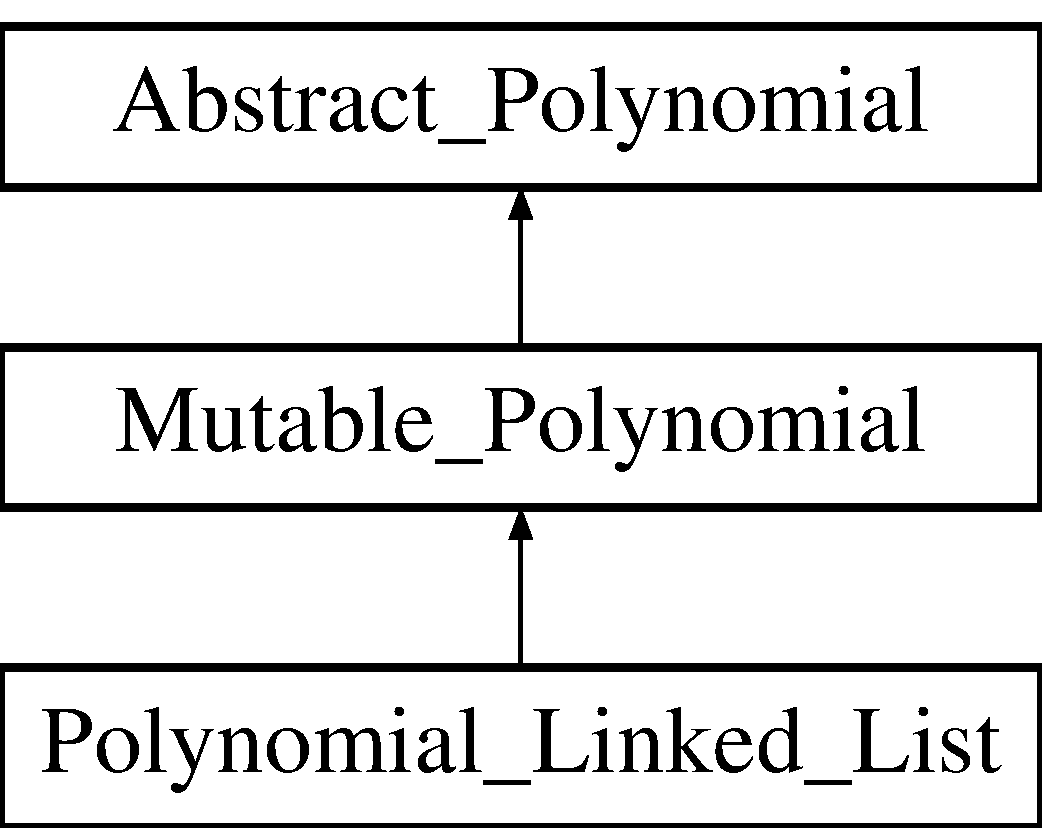
\includegraphics[height=3.000000cm]{group__polygroup}
\end{center}
\end{figure}
\subsubsection*{Public Member Functions}
\begin{Indent}\textbf{ Construction}\par
\begin{DoxyCompactItemize}
\item 
\mbox{\Hypertarget{group__polygroup_a251f514b92748997c7b66abb171196cd}\label{group__polygroup_a251f514b92748997c7b66abb171196cd}} 
\hyperlink{group__polygroup_a251f514b92748997c7b66abb171196cd}{Polynomial\+\_\+\+Linked\+\_\+\+List} (\hyperlink{group__polygroup_class_polynomial___ring}{Polynomial\+\_\+\+Ring} \&\hyperlink{group__polygroup_a551ade20b7dcd96c227dd0401f6ffbbe}{R}, const \hyperlink{group__orderinggroup_class_monomial___ordering}{Monomial\+\_\+\+Ordering} $\ast$order=generic\+\_\+grevlex\+\_\+ptr)
\begin{DoxyCompactList}\small\item\em initialize to zero \end{DoxyCompactList}\item 
\mbox{\Hypertarget{group__polygroup_a801c742fedba1aa99a0181d12d349cba}\label{group__polygroup_a801c742fedba1aa99a0181d12d349cba}} 
\hyperlink{group__polygroup_a801c742fedba1aa99a0181d12d349cba}{Polynomial\+\_\+\+Linked\+\_\+\+List} (\hyperlink{group__polygroup_class_polynomial___ring}{Polynomial\+\_\+\+Ring} \&\hyperlink{group__polygroup_a551ade20b7dcd96c227dd0401f6ffbbe}{R}, const \hyperlink{group__polygroup_class_monomial}{Monomial} \&t, const \hyperlink{group__orderinggroup_class_monomial___ordering}{Monomial\+\_\+\+Ordering} $\ast$order=nullptr)
\begin{DoxyCompactList}\small\item\em initialize to monomial; monomial is copied \end{DoxyCompactList}\item 
\mbox{\Hypertarget{group__polygroup_a85e7e2a93687e95f706d02d462b46fc6}\label{group__polygroup_a85e7e2a93687e95f706d02d462b46fc6}} 
\hyperlink{group__polygroup_a85e7e2a93687e95f706d02d462b46fc6}{Polynomial\+\_\+\+Linked\+\_\+\+List} (\hyperlink{group__polygroup_class_polynomial___ring}{Polynomial\+\_\+\+Ring} \&\hyperlink{group__polygroup_a551ade20b7dcd96c227dd0401f6ffbbe}{R}, const \hyperlink{group___fields_group_class_prime___field___element}{Prime\+\_\+\+Field\+\_\+\+Element} \&c, const \hyperlink{group__polygroup_class_monomial}{Monomial} \&t, const \hyperlink{group__orderinggroup_class_monomial___ordering}{Monomial\+\_\+\+Ordering} $\ast$order=nullptr)
\begin{DoxyCompactList}\small\item\em initialize to monomial and coefficient; monomial is copied \end{DoxyCompactList}\item 
\mbox{\Hypertarget{group__polygroup_a67949390f9d60f7cc3a0e9eef8b60e37}\label{group__polygroup_a67949390f9d60f7cc3a0e9eef8b60e37}} 
\hyperlink{group__polygroup_a67949390f9d60f7cc3a0e9eef8b60e37}{Polynomial\+\_\+\+Linked\+\_\+\+List} (\hyperlink{group__polygroup_class_polynomial___ring}{Polynomial\+\_\+\+Ring} \&\hyperlink{group__polygroup_a551ade20b7dcd96c227dd0401f6ffbbe}{R}, \hyperlink{group__polygroup_class_monomial___node}{Monomial\+\_\+\+Node} $\ast$node, const \hyperlink{group__orderinggroup_class_monomial___ordering}{Monomial\+\_\+\+Ordering} $\ast$order=nullptr)
\begin{DoxyCompactList}\small\item\em initialize to given monomial node\+: nothing is copied \end{DoxyCompactList}\item 
\mbox{\Hypertarget{group__polygroup_abd37d81f9f973f93d380425882b0b7d6}\label{group__polygroup_abd37d81f9f973f93d380425882b0b7d6}} 
\hyperlink{group__polygroup_abd37d81f9f973f93d380425882b0b7d6}{Polynomial\+\_\+\+Linked\+\_\+\+List} (const \hyperlink{group__polygroup_class_polynomial___linked___list}{Polynomial\+\_\+\+Linked\+\_\+\+List} \&other)
\begin{DoxyCompactList}\small\item\em copy constructor\+: deep copy of monomials \end{DoxyCompactList}\item 
\mbox{\Hypertarget{group__polygroup_a347fda55f27fa10327c9854913d416ce}\label{group__polygroup_a347fda55f27fa10327c9854913d416ce}} 
\hyperlink{group__polygroup_a347fda55f27fa10327c9854913d416ce}{Polynomial\+\_\+\+Linked\+\_\+\+List} (const \hyperlink{group__polygroup_class_abstract___polynomial}{Abstract\+\_\+\+Polynomial} \&p)
\begin{DoxyCompactList}\small\item\em constructor from abstract polynomial\+: deep copy of monomials \end{DoxyCompactList}\end{DoxyCompactItemize}
\end{Indent}
\begin{Indent}\textbf{ Destruction}\par
\begin{DoxyCompactItemize}
\item 
\mbox{\Hypertarget{group__polygroup_a02235c20d279afa443ea836fd9336cfc}\label{group__polygroup_a02235c20d279afa443ea836fd9336cfc}} 
virtual \hyperlink{group__polygroup_a02235c20d279afa443ea836fd9336cfc}{$\sim$\+Polynomial\+\_\+\+Linked\+\_\+\+List} ()
\begin{DoxyCompactList}\small\item\em deletes all monomial nodes \end{DoxyCompactList}\end{DoxyCompactItemize}
\end{Indent}
\begin{Indent}\textbf{ Basic properties}\par
\begin{DoxyCompactItemize}
\item 
\mbox{\Hypertarget{group__polygroup_a47ca76404bf5c97d1dadbf6c96638ac5}\label{group__polygroup_a47ca76404bf5c97d1dadbf6c96638ac5}} 
virtual bool \hyperlink{group__polygroup_a47ca76404bf5c97d1dadbf6c96638ac5}{is\+\_\+zero} () const override
\begin{DoxyCompactList}\small\item\em true iff the first node in the list is {\ttfamily nullptr} or has zero coeff \end{DoxyCompactList}\item 
\mbox{\Hypertarget{group__polygroup_aa2e4fe2b54a3da9074d3708f2a4729b7}\label{group__polygroup_aa2e4fe2b54a3da9074d3708f2a4729b7}} 
virtual \hyperlink{group__polygroup_class_monomial}{Monomial} \& \hyperlink{group__polygroup_aa2e4fe2b54a3da9074d3708f2a4729b7}{leading\+\_\+monomial} () const override
\begin{DoxyCompactList}\small\item\em Returns the leading monomial --- call \hyperlink{group__polygroup_a254bec60707b34bd26ef9d9bb08a4fe9}{sort\+\_\+by\+\_\+order()} first! \end{DoxyCompactList}\item 
\mbox{\Hypertarget{group__polygroup_a34df585ea11a657b4cfbdf18b6ba8434}\label{group__polygroup_a34df585ea11a657b4cfbdf18b6ba8434}} 
virtual \hyperlink{group___fields_group_class_prime___field___element}{Prime\+\_\+\+Field\+\_\+\+Element} \hyperlink{group__polygroup_a34df585ea11a657b4cfbdf18b6ba8434}{leading\+\_\+coefficient} () const override
\begin{DoxyCompactList}\small\item\em Returns the leading coefficient --- call sort\+\_\+by\+\_\+order first! \end{DoxyCompactList}\item 
\mbox{\Hypertarget{group__polygroup_a5bb88b639d9083ba8c84c576f8aaf0e7}\label{group__polygroup_a5bb88b639d9083ba8c84c576f8aaf0e7}} 
virtual unsigned \hyperlink{group__polygroup_a5bb88b639d9083ba8c84c576f8aaf0e7}{length} () const override
\begin{DoxyCompactList}\small\item\em Returns the number of polynomials in the list. \end{DoxyCompactList}\item 
virtual void \hyperlink{group__polygroup_af9b1dee3a8ca9fb26a6e069ea70ea5df}{set\+\_\+monomial\+\_\+ordering} (const \hyperlink{group__orderinggroup_class_monomial___ordering}{Monomial\+\_\+\+Ordering} $\ast$ord, bool sort\+\_\+anew=true) override
\begin{DoxyCompactList}\small\item\em set the monomial ordering and sort the polynomials (optionally, but by default) \end{DoxyCompactList}\end{DoxyCompactItemize}
\end{Indent}
\begin{Indent}\textbf{ Computation}\par
\begin{DoxyCompactItemize}
\item 
\mbox{\Hypertarget{group__polygroup_afef3be2bfef96bffcc069c95147e1d03}\label{group__polygroup_afef3be2bfef96bffcc069c95147e1d03}} 
virtual \hyperlink{group__polygroup_class_polynomial___linked___list}{Polynomial\+\_\+\+Linked\+\_\+\+List} $\ast$ \hyperlink{group__polygroup_afef3be2bfef96bffcc069c95147e1d03}{zero\+\_\+polynomial} () const override
\begin{DoxyCompactList}\small\item\em Returns as simple a zero polynomial as I can muster, short of this being {\ttfamily nullptr}. \end{DoxyCompactList}\item 
\mbox{\Hypertarget{group__polygroup_abb11e27691b50b0ef6edc87d5b041af5}\label{group__polygroup_abb11e27691b50b0ef6edc87d5b041af5}} 
virtual \hyperlink{group__polygroup_class_polynomial___linked___list}{Polynomial\+\_\+\+Linked\+\_\+\+List} $\ast$ \hyperlink{group__polygroup_abb11e27691b50b0ef6edc87d5b041af5}{monomial\+\_\+multiple} (const \hyperlink{group__polygroup_class_monomial}{Monomial} \&u) const override
\begin{DoxyCompactList}\small\item\em Returns a new polynomial whose value is $\textit{this}\times u$. \end{DoxyCompactList}\item 
\mbox{\Hypertarget{group__polygroup_af2df2928edc94ab86e9ded43a9f967f5}\label{group__polygroup_af2df2928edc94ab86e9ded43a9f967f5}} 
virtual \hyperlink{group__polygroup_class_polynomial___linked___list}{Polynomial\+\_\+\+Linked\+\_\+\+List} $\ast$ \hyperlink{group__polygroup_af2df2928edc94ab86e9ded43a9f967f5}{scalar\+\_\+multiple} (const \hyperlink{group___fields_group_class_prime___field___element}{Prime\+\_\+\+Field\+\_\+\+Element} \&c) const override
\begin{DoxyCompactList}\small\item\em Returns a new polynomial whose value is $\textit{this}\times c$. \end{DoxyCompactList}\item 
\mbox{\Hypertarget{group__polygroup_aafbd4195047ae999f1a5674d34797431}\label{group__polygroup_aafbd4195047ae999f1a5674d34797431}} 
virtual \hyperlink{group__polygroup_class_polynomial___linked___list}{Polynomial\+\_\+\+Linked\+\_\+\+List} \& \hyperlink{group__polygroup_aafbd4195047ae999f1a5674d34797431}{operator+=} (const \hyperlink{group__polygroup_class_abstract___polynomial}{Abstract\+\_\+\+Polynomial} \&other) override
\begin{DoxyCompactList}\small\item\em Adds {\ttfamily other} to {\ttfamily this}, and returns the result. \end{DoxyCompactList}\item 
\mbox{\Hypertarget{group__polygroup_a80f13f9bdcabb034c83c243fd0bdc004}\label{group__polygroup_a80f13f9bdcabb034c83c243fd0bdc004}} 
virtual \hyperlink{group__polygroup_class_polynomial___linked___list}{Polynomial\+\_\+\+Linked\+\_\+\+List} \& \hyperlink{group__polygroup_a80f13f9bdcabb034c83c243fd0bdc004}{operator-\/=} (const \hyperlink{group__polygroup_class_abstract___polynomial}{Abstract\+\_\+\+Polynomial} \&other) override
\begin{DoxyCompactList}\small\item\em Subtracts {\ttfamily other} from {\ttfamily this}, and returns the result. \end{DoxyCompactList}\item 
virtual void \hyperlink{group__polygroup_a610a577011774265552efb30508ece94}{add\+\_\+polynomial\+\_\+multiple} (const \hyperlink{group___fields_group_class_prime___field___element}{Prime\+\_\+\+Field\+\_\+\+Element} \&a, const \hyperlink{group__polygroup_class_monomial}{Monomial} \&t, const \hyperlink{group__polygroup_class_abstract___polynomial}{Abstract\+\_\+\+Polynomial} \&q, bool subtract) override
\begin{DoxyCompactList}\small\item\em \char`\"{}\+Fast\char`\"{} addition of $atq$ to {\ttfamily this}. \end{DoxyCompactList}\item 
\mbox{\Hypertarget{group__polygroup_a254bec60707b34bd26ef9d9bb08a4fe9}\label{group__polygroup_a254bec60707b34bd26ef9d9bb08a4fe9}} 
virtual void \hyperlink{group__polygroup_a254bec60707b34bd26ef9d9bb08a4fe9}{sort\+\_\+by\+\_\+order} () override
\begin{DoxyCompactList}\small\item\em Sort by specified weight order. \end{DoxyCompactList}\end{DoxyCompactItemize}
\end{Indent}
\begin{Indent}\textbf{ Iteration}\par
\begin{DoxyCompactItemize}
\item 
\mbox{\Hypertarget{group__polygroup_ac17e14ceb70ee8862e044ad6b44a78a5}\label{group__polygroup_ac17e14ceb70ee8862e044ad6b44a78a5}} 
virtual \hyperlink{group___iterator_group_class_l_l_polynomial___iterator}{L\+L\+Polynomial\+\_\+\+Iterator} $\ast$ \hyperlink{group__polygroup_ac17e14ceb70ee8862e044ad6b44a78a5}{new\+\_\+iterator} () const override
\begin{DoxyCompactList}\small\item\em an iterator that poses no risk of modifying the polynomial \end{DoxyCompactList}\item 
\mbox{\Hypertarget{group__polygroup_a32a8c930f367bf556b27e37c5cf0d2e7}\label{group__polygroup_a32a8c930f367bf556b27e37c5cf0d2e7}} 
virtual \hyperlink{group___iterator_group_class_polynomial___iterator}{Polynomial\+\_\+\+Iterator} $\ast$ \hyperlink{group__polygroup_a32a8c930f367bf556b27e37c5cf0d2e7}{begin} () const override
\begin{DoxyCompactList}\small\item\em an iterator that poses no risk of modifying the polynomial \end{DoxyCompactList}\item 
\mbox{\Hypertarget{group__polygroup_af38eba4370d879ae4603d3049c588d6c}\label{group__polygroup_af38eba4370d879ae4603d3049c588d6c}} 
virtual \hyperlink{group___iterator_group_class_polynomial___iterator}{Polynomial\+\_\+\+Iterator} $\ast$ \hyperlink{group__polygroup_af38eba4370d879ae4603d3049c588d6c}{end} () const override
\begin{DoxyCompactList}\small\item\em an iterator that poses no risk of modifying the polynomial \end{DoxyCompactList}\item 
\mbox{\Hypertarget{group__polygroup_a9a661c20acf3bedbecbb2acdce2598ab}\label{group__polygroup_a9a661c20acf3bedbecbb2acdce2598ab}} 
virtual \hyperlink{group___iterator_group_class_l_l_polynomial___iterator}{L\+L\+Polynomial\+\_\+\+Iterator} $\ast$ \hyperlink{group__polygroup_a9a661c20acf3bedbecbb2acdce2598ab}{new\+\_\+mutable\+\_\+iterator} () override
\begin{DoxyCompactList}\small\item\em An iterator that may modify the current position. \end{DoxyCompactList}\end{DoxyCompactItemize}
\end{Indent}
\begin{Indent}\textbf{ Modification}\par
\begin{DoxyCompactItemize}
\item 
\mbox{\Hypertarget{group__polygroup_a919a99403d3e5117919b3086844cb0e8}\label{group__polygroup_a919a99403d3e5117919b3086844cb0e8}} 
virtual \hyperlink{group__polygroup_class_polynomial___linked___list}{Polynomial\+\_\+\+Linked\+\_\+\+List} $\ast$ \hyperlink{group__polygroup_a919a99403d3e5117919b3086844cb0e8}{detach\+\_\+head} () override
\begin{DoxyCompactList}\small\item\em Detach and return leading term. \end{DoxyCompactList}\item 
\mbox{\Hypertarget{group__polygroup_a03ec271b09917f4dbabfe695fffad0ea}\label{group__polygroup_a03ec271b09917f4dbabfe695fffad0ea}} 
virtual void \hyperlink{group__polygroup_a03ec271b09917f4dbabfe695fffad0ea}{add\+\_\+last} (const \hyperlink{group___fields_group_class_prime___field___element}{Prime\+\_\+\+Field\+\_\+\+Element} \&c, const \hyperlink{group__polygroup_class_monomial}{Monomial} \&t) override
\begin{DoxyCompactList}\small\item\em Add this monomial as the last leading term. \end{DoxyCompactList}\end{DoxyCompactItemize}
\end{Indent}
\subsubsection*{Protected Attributes}
\begin{DoxyCompactItemize}
\item 
\mbox{\Hypertarget{group__polygroup_a55c2905ab5c77fb51ff1c282ec3ce9e5}\label{group__polygroup_a55c2905ab5c77fb51ff1c282ec3ce9e5}} 
\hyperlink{group__polygroup_class_monomial___node}{Monomial\+\_\+\+Node} $\ast$ \hyperlink{group__polygroup_a55c2905ab5c77fb51ff1c282ec3ce9e5}{head}
\begin{DoxyCompactList}\small\item\em first monomial in the list, returned by \hyperlink{group__polygroup_aa2e4fe2b54a3da9074d3708f2a4729b7}{leading\+\_\+monomial()} \end{DoxyCompactList}\end{DoxyCompactItemize}
\subsubsection*{Friends}
\begin{DoxyCompactItemize}
\item 
\mbox{\Hypertarget{group__polygroup_adc04ceaa684cbc36bd6800c57364bd2e}\label{group__polygroup_adc04ceaa684cbc36bd6800c57364bd2e}} 
class \hyperlink{group__polygroup_adc04ceaa684cbc36bd6800c57364bd2e}{L\+L\+Polynomial\+\_\+\+Iterator}
\begin{DoxyCompactList}\small\item\em to iterate over {\ttfamily this} and possibly change it \end{DoxyCompactList}\end{DoxyCompactItemize}


\paragraph{Member Function Documentation}
\mbox{\Hypertarget{group__polygroup_a610a577011774265552efb30508ece94}\label{group__polygroup_a610a577011774265552efb30508ece94}} 
\index{Polynomial\+\_\+\+Linked\+\_\+\+List@{Polynomial\+\_\+\+Linked\+\_\+\+List}!add\+\_\+polynomial\+\_\+multiple@{add\+\_\+polynomial\+\_\+multiple}}
\index{add\+\_\+polynomial\+\_\+multiple@{add\+\_\+polynomial\+\_\+multiple}!Polynomial\+\_\+\+Linked\+\_\+\+List@{Polynomial\+\_\+\+Linked\+\_\+\+List}}
\subparagraph{\texorpdfstring{add\+\_\+polynomial\+\_\+multiple()}{add\_polynomial\_multiple()}}
{\footnotesize\ttfamily void Polynomial\+\_\+\+Linked\+\_\+\+List\+::add\+\_\+polynomial\+\_\+multiple (\begin{DoxyParamCaption}\item[{const \hyperlink{group___fields_group_class_prime___field___element}{Prime\+\_\+\+Field\+\_\+\+Element} \&}]{a,  }\item[{const \hyperlink{group__polygroup_class_monomial}{Monomial} \&}]{t,  }\item[{const \hyperlink{group__polygroup_class_abstract___polynomial}{Abstract\+\_\+\+Polynomial} \&}]{q,  }\item[{bool}]{subtract }\end{DoxyParamCaption})\hspace{0.3cm}{\ttfamily [override]}, {\ttfamily [virtual]}}



\char`\"{}\+Fast\char`\"{} addition of $atq$ to {\ttfamily this}. 

If {\ttfamily subtract==true}, subtract instead. 
\begin{DoxyParams}{Parameters}
{\em a} & coefficient of the term to multiply to {\ttfamily q} \\
\hline
{\em t} & \hyperlink{group__polygroup_class_monomial}{Monomial} of the term to multiply to {\ttfamily q} \\
\hline
{\em q} & polynomial to add to {\ttfamily this}, after multiplying {\ttfamily q} by $ at $ \\
\hline
{\em subtract} & whether to add instead of subtract \\
\hline
\end{DoxyParams}


Implements \hyperlink{group__polygroup_add21309f55af6a58e1d9b1623a0bb09a}{Mutable\+\_\+\+Polynomial}.



Definition at line 389 of file polynomial\+\_\+linked\+\_\+list.\+cpp.

\mbox{\Hypertarget{group__polygroup_af9b1dee3a8ca9fb26a6e069ea70ea5df}\label{group__polygroup_af9b1dee3a8ca9fb26a6e069ea70ea5df}} 
\index{Polynomial\+\_\+\+Linked\+\_\+\+List@{Polynomial\+\_\+\+Linked\+\_\+\+List}!set\+\_\+monomial\+\_\+ordering@{set\+\_\+monomial\+\_\+ordering}}
\index{set\+\_\+monomial\+\_\+ordering@{set\+\_\+monomial\+\_\+ordering}!Polynomial\+\_\+\+Linked\+\_\+\+List@{Polynomial\+\_\+\+Linked\+\_\+\+List}}
\subparagraph{\texorpdfstring{set\+\_\+monomial\+\_\+ordering()}{set\_monomial\_ordering()}}
{\footnotesize\ttfamily void Polynomial\+\_\+\+Linked\+\_\+\+List\+::set\+\_\+monomial\+\_\+ordering (\begin{DoxyParamCaption}\item[{const \hyperlink{group__orderinggroup_class_monomial___ordering}{Monomial\+\_\+\+Ordering} $\ast$}]{order,  }\item[{bool}]{sort\+\_\+anew = {\ttfamily true} }\end{DoxyParamCaption})\hspace{0.3cm}{\ttfamily [override]}, {\ttfamily [virtual]}}



set the monomial ordering and sort the polynomials (optionally, but by default) 


\begin{DoxyParams}{Parameters}
{\em order} & new monomial ordering \\
\hline
{\em sort\+\_\+anew} & whether to sort the polynomial anew \\
\hline
\end{DoxyParams}
\begin{DoxyWarning}{Warning}
In most cases you will want to sort anew {\itshape immediately} after setting the ordering. Otherwise, the monomials may be in the wrong order! That is therefore the default behavior of this function, but in case you don't want to sort, that option is provided. 
\end{DoxyWarning}


Implements \hyperlink{group__polygroup_a12e023570eb675343c4b7ed635a031dc}{Abstract\+\_\+\+Polynomial}.



Definition at line 232 of file polynomial\+\_\+linked\+\_\+list.\+cpp.

\index{Polynomial\+\_\+\+Ring@{Polynomial\+\_\+\+Ring}}\label{class_polynomial___ring}
\Hypertarget{group__polygroup_class_polynomial___ring}
\subsubsection{class Polynomial\+\_\+\+Ring}
Encapsulates information about a polynomial ring for easy access\+: ground field, number of indeterminates, {$\dots$}. 

\begin{DoxyAuthor}{Author}
John Perry 
\end{DoxyAuthor}
\begin{DoxyDate}{Date}
2015 
\end{DoxyDate}
\begin{Desc}
\item[Examples\+: ]\par
\hyperlink{test_4by4_8cpp-example}{test\+\_\+4by4.\+cpp}, \hyperlink{test_cab_es1_8cpp-example}{test\+\_\+cab\+\_\+es1.\+cpp}, \hyperlink{test_cab_es2_8cpp-example}{test\+\_\+cab\+\_\+es2.\+cpp}, \hyperlink{test_cab_es4_8cpp-example}{test\+\_\+cab\+\_\+es4.\+cpp}, \hyperlink{test_cab_es5_8cpp-example}{test\+\_\+cab\+\_\+es5.\+cpp}, \hyperlink{test_cab_es6_8cpp-example}{test\+\_\+cab\+\_\+es6.\+cpp}, \hyperlink{test_cab_es9_8cpp-example}{test\+\_\+cab\+\_\+es9.\+cpp}, \hyperlink{test_cyclic4_8cpp-example}{test\+\_\+cyclic4.\+cpp}, \hyperlink{test_cyclicn_8cpp-example}{test\+\_\+cyclicn.\+cpp}, \hyperlink{test_dynamic_8cpp-example}{test\+\_\+dynamic.\+cpp}, \hyperlink{test_f4_8cpp-example}{test\+\_\+f4.\+cpp}, \hyperlink{test_f4_dynamic_8cpp-example}{test\+\_\+f4\+\_\+dynamic.\+cpp}, \hyperlink{test_monomials_8cpp-example}{test\+\_\+monomials.\+cpp}, and \hyperlink{user_interface_8cpp-example}{user\+\_\+interface.\+cpp}.\end{Desc}


Definition at line 42 of file polynomial\+\_\+ring.\+hpp.

\subsubsection*{Public Member Functions}
\begin{Indent}\textbf{ Construction}\par
\begin{DoxyCompactItemize}
\item 
\hyperlink{group__polygroup_af62688669a31cb720bb1e90a724daa4f}{Polynomial\+\_\+\+Ring} (N\+V\+A\+R\+\_\+\+T\+Y\+PE num\+\_\+vars, \hyperlink{group___fields_group_class_prime___field}{Prime\+\_\+\+Field} \&field, string $\ast$var\+\_\+names=nullptr)
\begin{DoxyCompactList}\small\item\em Initialize the ring for the given field and number of indeterminates. \end{DoxyCompactList}\end{DoxyCompactItemize}
\end{Indent}
\begin{Indent}\textbf{ Destruction}\par
\begin{DoxyCompactItemize}
\item 
\mbox{\Hypertarget{group__polygroup_ac4952692f32f57ccd3a7e68e20cb3662}\label{group__polygroup_ac4952692f32f57ccd3a7e68e20cb3662}} 
\hyperlink{group__polygroup_ac4952692f32f57ccd3a7e68e20cb3662}{$\sim$\+Polynomial\+\_\+\+Ring} ()
\begin{DoxyCompactList}\small\item\em Deletes the names. \end{DoxyCompactList}\end{DoxyCompactItemize}
\end{Indent}
\begin{Indent}\textbf{ Modification}\par
\begin{DoxyCompactItemize}
\item 
bool \hyperlink{group__polygroup_ae59dcd21a16ffccc7b32e3c2f898b6f3}{set\+\_\+names} (string $\ast$new\+\_\+names, N\+V\+A\+R\+\_\+\+T\+Y\+PE length)
\begin{DoxyCompactList}\small\item\em sets the names of the indeterminates, if you do not want the default \end{DoxyCompactList}\end{DoxyCompactItemize}
\end{Indent}
\begin{Indent}\textbf{ Basic properties}\par
\begin{DoxyCompactItemize}
\item 
\mbox{\Hypertarget{group__polygroup_a79e7dd821659e9d4b6862487963f7352}\label{group__polygroup_a79e7dd821659e9d4b6862487963f7352}} 
virtual N\+V\+A\+R\+\_\+\+T\+Y\+PE \hyperlink{group__polygroup_a79e7dd821659e9d4b6862487963f7352}{number\+\_\+of\+\_\+variables} () const
\begin{DoxyCompactList}\small\item\em number of indeterminates (variables) in the ring \end{DoxyCompactList}\item 
\mbox{\Hypertarget{group__polygroup_afea6c3a4fd9f3f04f312579a94a3cc1b}\label{group__polygroup_afea6c3a4fd9f3f04f312579a94a3cc1b}} 
virtual \hyperlink{group__polygroup_class_indeterminate}{Indeterminate} $\ast$ \hyperlink{group__polygroup_afea6c3a4fd9f3f04f312579a94a3cc1b}{indeterminates} ()
\begin{DoxyCompactList}\small\item\em an array of the ring's indeterminates; use only to biuld polynomials \end{DoxyCompactList}\item 
\mbox{\Hypertarget{group__polygroup_a643bd55dbe8686b2dd1341503a67aace}\label{group__polygroup_a643bd55dbe8686b2dd1341503a67aace}} 
virtual \hyperlink{group___fields_group_class_prime___field}{Prime\+\_\+\+Field} \& \hyperlink{group__polygroup_a643bd55dbe8686b2dd1341503a67aace}{ground\+\_\+field} () const
\begin{DoxyCompactList}\small\item\em ground field \end{DoxyCompactList}\item 
\mbox{\Hypertarget{group__polygroup_a657caa3e9c277ca34d20cb69eed7fe05}\label{group__polygroup_a657caa3e9c277ca34d20cb69eed7fe05}} 
virtual const string \hyperlink{group__polygroup_a657caa3e9c277ca34d20cb69eed7fe05}{name} (N\+V\+A\+R\+\_\+\+T\+Y\+PE i) const
\begin{DoxyCompactList}\small\item\em name of the $i$th indeterminate \end{DoxyCompactList}\item 
\mbox{\Hypertarget{group__polygroup_aef9c6745956393863080422ddb8da48c}\label{group__polygroup_aef9c6745956393863080422ddb8da48c}} 
virtual const string $\ast$ \hyperlink{group__polygroup_aef9c6745956393863080422ddb8da48c}{name\+\_\+list} () const
\begin{DoxyCompactList}\small\item\em names of all the variabiles \end{DoxyCompactList}\end{DoxyCompactItemize}
\end{Indent}
\subsubsection*{Protected Attributes}
\begin{DoxyCompactItemize}
\item 
\mbox{\Hypertarget{group__polygroup_a99cdb13a26bf70032c19fe01a3cea1d8}\label{group__polygroup_a99cdb13a26bf70032c19fe01a3cea1d8}} 
\hyperlink{group___fields_group_class_prime___field}{Prime\+\_\+\+Field} \& \hyperlink{group__polygroup_a99cdb13a26bf70032c19fe01a3cea1d8}{F}
\begin{DoxyCompactList}\small\item\em the ring\textquotesingle{}s ground field \end{DoxyCompactList}\item 
N\+V\+A\+R\+\_\+\+T\+Y\+PE \hyperlink{group__polygroup_abf753b41b3e84bd8e32de314f15f7826}{n}
\begin{DoxyCompactList}\small\item\em the number of indeterminates for every monomial in the ring \end{DoxyCompactList}\item 
\mbox{\Hypertarget{group__polygroup_ad7634678157b109f713da3a712f2af35}\label{group__polygroup_ad7634678157b109f713da3a712f2af35}} 
string $\ast$ \hyperlink{group__polygroup_ad7634678157b109f713da3a712f2af35}{names}
\begin{DoxyCompactList}\small\item\em optional names for the variables \end{DoxyCompactList}\end{DoxyCompactItemize}


\paragraph{Constructor \& Destructor Documentation}
\mbox{\Hypertarget{group__polygroup_af62688669a31cb720bb1e90a724daa4f}\label{group__polygroup_af62688669a31cb720bb1e90a724daa4f}} 
\index{Polynomial\+\_\+\+Ring@{Polynomial\+\_\+\+Ring}!Polynomial\+\_\+\+Ring@{Polynomial\+\_\+\+Ring}}
\index{Polynomial\+\_\+\+Ring@{Polynomial\+\_\+\+Ring}!Polynomial\+\_\+\+Ring@{Polynomial\+\_\+\+Ring}}
\subparagraph{\texorpdfstring{Polynomial\+\_\+\+Ring()}{Polynomial\_Ring()}}
{\footnotesize\ttfamily Polynomial\+\_\+\+Ring\+::\+Polynomial\+\_\+\+Ring (\begin{DoxyParamCaption}\item[{N\+V\+A\+R\+\_\+\+T\+Y\+PE}]{num\+\_\+vars,  }\item[{\hyperlink{group___fields_group_class_prime___field}{Prime\+\_\+\+Field} \&}]{field,  }\item[{string $\ast$}]{var\+\_\+names = {\ttfamily nullptr} }\end{DoxyParamCaption})}



Initialize the ring for the given field and number of indeterminates. 

The array of names is copied, so you can reuse or discard the memory as you prefer. 
\begin{DoxyParams}{Parameters}
{\em num\+\_\+vars} & number of indeterminates in this \hyperlink{group__polygroup_class_polynomial___ring}{Polynomial\+\_\+\+Ring} \\
\hline
{\em field} & ground field of this \hyperlink{group__polygroup_class_polynomial___ring}{Polynomial\+\_\+\+Ring} \\
\hline
{\em var\+\_\+names} & an optional array of {\ttfamily num\+\_\+vars} names to assign to the indeterminates \\
\hline
\end{DoxyParams}


Definition at line 25 of file polynomial\+\_\+ring.\+cpp.



\paragraph{Member Function Documentation}
\mbox{\Hypertarget{group__polygroup_ae59dcd21a16ffccc7b32e3c2f898b6f3}\label{group__polygroup_ae59dcd21a16ffccc7b32e3c2f898b6f3}} 
\index{Polynomial\+\_\+\+Ring@{Polynomial\+\_\+\+Ring}!set\+\_\+names@{set\+\_\+names}}
\index{set\+\_\+names@{set\+\_\+names}!Polynomial\+\_\+\+Ring@{Polynomial\+\_\+\+Ring}}
\subparagraph{\texorpdfstring{set\+\_\+names()}{set\_names()}}
{\footnotesize\ttfamily bool Polynomial\+\_\+\+Ring\+::set\+\_\+names (\begin{DoxyParamCaption}\item[{string $\ast$}]{new\+\_\+names,  }\item[{N\+V\+A\+R\+\_\+\+T\+Y\+PE}]{length }\end{DoxyParamCaption})}



sets the names of the indeterminates, if you do not want the default 

Returns {\ttfamily True} if and only if successful. The names are not copied, so please do not discard them until you are done with this ring, or else have reassigned the names. \begin{DoxyWarning}{Warning}
If {\ttfamily length} is not the same as the number of indeterminates, things can go very, very badly. 
\end{DoxyWarning}

\begin{DoxyParams}{Parameters}
{\em new\+\_\+names} & names for the indeterminates \\
\hline
{\em length} & number of names in {\ttfamily new\+\_\+names} \\
\hline
\end{DoxyParams}
\begin{DoxyReturn}{Returns}
whether all supplied names were set 
\end{DoxyReturn}


Definition at line 40 of file polynomial\+\_\+ring.\+cpp.



\paragraph{Member Data Documentation}
\mbox{\Hypertarget{group__polygroup_abf753b41b3e84bd8e32de314f15f7826}\label{group__polygroup_abf753b41b3e84bd8e32de314f15f7826}} 
\index{Polynomial\+\_\+\+Ring@{Polynomial\+\_\+\+Ring}!n@{n}}
\index{n@{n}!Polynomial\+\_\+\+Ring@{Polynomial\+\_\+\+Ring}}
\subparagraph{\texorpdfstring{n}{n}}
{\footnotesize\ttfamily N\+V\+A\+R\+\_\+\+T\+Y\+PE Polynomial\+\_\+\+Ring\+::n\hspace{0.3cm}{\ttfamily [protected]}}



the number of indeterminates for every monomial in the ring 

\begin{DoxyWarning}{Warning}
The system does not verify that the number of indeterminates in a monomial agrees with the number specified in this ring. This information is easily available through the \hyperlink{group__polygroup_a79e7dd821659e9d4b6862487963f7352}{number\+\_\+of\+\_\+variables()} command. 
\end{DoxyWarning}


Definition at line 102 of file polynomial\+\_\+ring.\+hpp.



\subsection{Function Documentation}
\mbox{\Hypertarget{group__polygroup_gaf4655e829836ead5fe2ce766fb0cebbc}\label{group__polygroup_gaf4655e829836ead5fe2ce766fb0cebbc}} 
\index{Polynomials@{Polynomials}!colon\+\_\+ideal\+\_\+without\+\_\+ideals@{colon\+\_\+ideal\+\_\+without\+\_\+ideals}}
\index{colon\+\_\+ideal\+\_\+without\+\_\+ideals@{colon\+\_\+ideal\+\_\+without\+\_\+ideals}!Polynomials@{Polynomials}}
\subsubsection{\texorpdfstring{colon\+\_\+ideal\+\_\+without\+\_\+ideals()}{colon\_ideal\_without\_ideals()}}
{\footnotesize\ttfamily list$<$\hyperlink{group__polygroup_class_monomial}{Monomial}$>$ colon\+\_\+ideal\+\_\+without\+\_\+ideals (\begin{DoxyParamCaption}\item[{const list$<$ \hyperlink{group__polygroup_class_monomial}{Monomial} $>$ \&}]{U,  }\item[{const \hyperlink{group__polygroup_class_monomial}{Monomial} \&}]{t }\end{DoxyParamCaption})}



Computes the generators of an ideal and a new generator, given the ideal\textquotesingle{}s generators. No monomial ideal machinery required. 

\begin{DoxyAuthor}{Author}
John Perry 
\end{DoxyAuthor}
\begin{DoxyDate}{Date}
2016 
\end{DoxyDate}

\begin{DoxyParams}{Parameters}
{\em U} & generators of ideal we want to ``colonize'' \\
\hline
{\em t} & \hyperlink{group__polygroup_class_monomial}{Monomial} that is ``colonizing'' the ideal generated by {\ttfamily U} \\
\hline
\end{DoxyParams}
\begin{DoxyReturn}{Returns}
a list of generators of the colon ideal of {\ttfamily U} by {\ttfamily t} ( $ U:(t) $) 
\end{DoxyReturn}


Definition at line 42 of file monomial\+\_\+ideal.\+cpp.

\mbox{\Hypertarget{group__polygroup_gaa458dfbf51ecbb98f93bf8f0133725d0}\label{group__polygroup_gaa458dfbf51ecbb98f93bf8f0133725d0}} 
\index{Polynomials@{Polynomials}!cyclic\+\_\+n@{cyclic\+\_\+n}}
\index{cyclic\+\_\+n@{cyclic\+\_\+n}!Polynomials@{Polynomials}}
\subsubsection{\texorpdfstring{cyclic\+\_\+n()}{cyclic\_n()}}
{\footnotesize\ttfamily list$<$\hyperlink{group__polygroup_class_abstract___polynomial}{Abstract\+\_\+\+Polynomial} $\ast$$>$ cyclic\+\_\+n (\begin{DoxyParamCaption}\item[{N\+V\+A\+R\+\_\+\+T\+Y\+PE}]{n,  }\item[{\hyperlink{group___fields_group_class_prime___field}{Prime\+\_\+\+Field} \&}]{F,  }\item[{bool}]{homog,  }\item[{\hyperlink{group__orderinggroup_class_monomial___ordering}{Monomial\+\_\+\+Ordering} $\ast$}]{mord = {\ttfamily generic\+\_\+grevlex\+\_\+ptr} }\end{DoxyParamCaption})}



generates the Cyclic-\/ $ n $ system 

\begin{DoxyReturn}{Returns}
a set of generators of the Cyclic-\/ $ n $ system, as pointers to \hyperlink{group__polygroup_class_constant___polynomial}{Constant\+\_\+\+Polynomial} 
\end{DoxyReturn}

\begin{DoxyParams}{Parameters}
{\em n} & number of variables \\
\hline
{\em F} & ground field \\
\hline
{\em homog} & whether to homogenize the system (affects only the last polynomial) \\
\hline
{\em mord} & a \hyperlink{group__orderinggroup_class_monomial___ordering}{Monomial\+\_\+\+Ordering}\\
\hline
\end{DoxyParams}
Generates the Cyclic-\/ $ n $ system, \[ x_0 + x_1 + ... + x_n,\\ x_0 x_1 + x_1 x_2 + x_2 x_3 + ... + x_n x_1,\\ x_0 x_1 x_2 + x_1 x_2 x_3 + x_2 x_3 x_4 + x_n x_1 x_2,\\ \ldots\\ x_0 x_1 \ldots x_n - 1.\] Use $n > 2$. If {\ttfamily homog} is {\ttfamily true}, the last monomial is $h^5$ instead of 1. \begin{Desc}
\item[Examples\+: ]\par
\hyperlink{test_cyclicn_8cpp-example}{test\+\_\+cyclicn.\+cpp}, \hyperlink{test_dynamic_8cpp-example}{test\+\_\+dynamic.\+cpp}, \hyperlink{test_f4_8cpp-example}{test\+\_\+f4.\+cpp}, and \hyperlink{test_f4_dynamic_8cpp-example}{test\+\_\+f4\+\_\+dynamic.\+cpp}.\end{Desc}


Definition at line 57 of file cyclic\+\_\+n.\+hpp.


\hypertarget{group__strategygroup}{}\section{Strategies}
\label{group__strategygroup}\index{Strategies@{Strategies}}


strategies for Gr\"{o}bner basis computation  


\subsection*{Classes}
\begin{DoxyCompactItemize}
\item 
class \hyperlink{group__strategygroup_class_normal___strategy}{Normal\+\_\+\+Strategy}
\begin{DoxyCompactList}\small\item\em ordering critical pairs using the normal strategy  \hyperlink{group__strategygroup_class_normal___strategy}{More...}\end{DoxyCompactList}\item 
class \hyperlink{group__strategygroup_class_pair___strategy___data}{Pair\+\_\+\+Strategy\+\_\+\+Data}
\begin{DoxyCompactList}\small\item\em Structure for sorting critical pairs.  \hyperlink{group__strategygroup_class_pair___strategy___data}{More...}\end{DoxyCompactList}\item 
class \hyperlink{group__strategygroup_class_pair___sugar___data}{Pair\+\_\+\+Sugar\+\_\+\+Data}
\begin{DoxyCompactList}\small\item\em ordering critical pairs using the sugar strategy  \hyperlink{group__strategygroup_class_pair___sugar___data}{More...}\end{DoxyCompactList}\item 
class \hyperlink{group__strategygroup_class_pair___w_sugar___strategy}{Pair\+\_\+\+W\+Sugar\+\_\+\+Strategy}
\begin{DoxyCompactList}\small\item\em ordering critical pairs using the weighted sugar strategy  \hyperlink{group__strategygroup_class_pair___w_sugar___strategy}{More...}\end{DoxyCompactList}\item 
class \hyperlink{group__strategygroup_class_poly___strategy___data}{Poly\+\_\+\+Strategy\+\_\+\+Data}
\begin{DoxyCompactList}\small\item\em polynomial-\/related strategy data  \hyperlink{group__strategygroup_class_poly___strategy___data}{More...}\end{DoxyCompactList}\item 
class \hyperlink{group__strategygroup_class_poly___sugar___data}{Poly\+\_\+\+Sugar\+\_\+\+Data}
\begin{DoxyCompactList}\small\item\em polynomial-\/related data for a sugar strategy  \hyperlink{group__strategygroup_class_poly___sugar___data}{More...}\end{DoxyCompactList}\item 
class \hyperlink{group__strategygroup_class_poly___w_sugar___data}{Poly\+\_\+\+W\+Sugar\+\_\+\+Data}
\begin{DoxyCompactList}\small\item\em polynomial-\/related data for a weighted sugar strategy  \hyperlink{group__strategygroup_class_poly___w_sugar___data}{More...}\end{DoxyCompactList}\end{DoxyCompactItemize}
\subsection*{Enumerations}
\begin{DoxyCompactItemize}
\item 
enum \hyperlink{group__strategygroup_ga0ee6c8e033547330e6b89929730007f4}{Strategy\+Flags} \{ {\bfseries N\+O\+R\+M\+A\+L\+\_\+\+S\+T\+R\+A\+T\+E\+GY} = 1, 
{\bfseries S\+U\+G\+A\+R\+\_\+\+S\+T\+R\+A\+T\+E\+GY}, 
{\bfseries W\+S\+U\+G\+A\+R\+\_\+\+S\+T\+R\+A\+T\+E\+GY}
 \}\begin{DoxyCompactList}\small\item\em flag indicating which strategy to use for computation \end{DoxyCompactList}
\end{DoxyCompactItemize}


\subsection{Detailed Description}
strategies for Gr\"{o}bner basis computation 



\subsection{Class Documentation}
\index{Normal\+\_\+\+Strategy@{Normal\+\_\+\+Strategy}}\label{class_normal___strategy}
\Hypertarget{group__strategygroup_class_normal___strategy}
\subsubsection{class Normal\+\_\+\+Strategy}
ordering critical pairs using the normal strategy 

\begin{DoxyAuthor}{Author}
John Perry 
\end{DoxyAuthor}
\begin{DoxyDate}{Date}
2016 
\end{DoxyDate}


Definition at line 32 of file normal\+\_\+strategy.\+hpp.

Inheritance diagram for Normal\+\_\+\+Strategy\+:\begin{figure}[H]
\begin{center}
\leavevmode
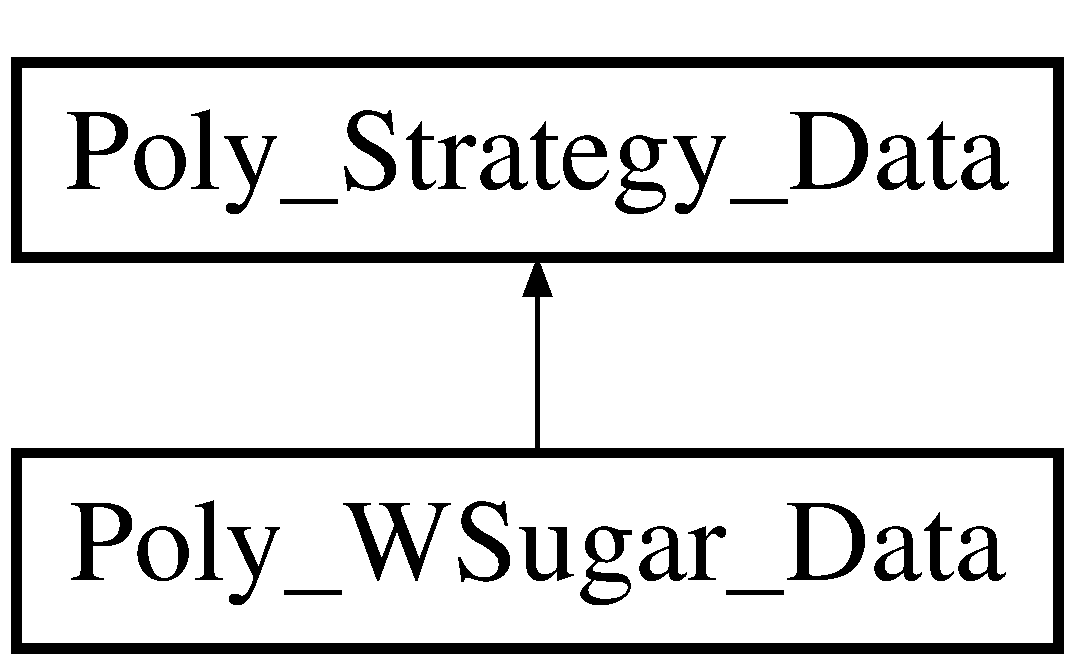
\includegraphics[height=2.000000cm]{group__strategygroup}
\end{center}
\end{figure}
\subsubsection*{Public Member Functions}
\begin{Indent}\textbf{ Construction}\par
\begin{DoxyCompactItemize}
\item 
\mbox{\Hypertarget{group__strategygroup_a6aa0afb9976f32afc9ae55d54d0ff9d4}\label{group__strategygroup_a6aa0afb9976f32afc9ae55d54d0ff9d4}} 
\hyperlink{group__strategygroup_a6aa0afb9976f32afc9ae55d54d0ff9d4}{Normal\+\_\+\+Strategy} (\hyperlink{group___g_b_computation_class_critical___pair___basic}{Critical\+\_\+\+Pair\+\_\+\+Basic} \&cpb)
\begin{DoxyCompactList}\small\item\em all the information we need is in {\ttfamily cpb} already so no additional processing is necessary \end{DoxyCompactList}\end{DoxyCompactItemize}
\end{Indent}
\begin{Indent}\textbf{ Comparison}\par
\begin{DoxyCompactItemize}
\item 
\mbox{\Hypertarget{group__strategygroup_a0e45af746d30c9608f48267aa2abb8d8}\label{group__strategygroup_a0e45af746d30c9608f48267aa2abb8d8}} 
virtual bool \hyperlink{group__strategygroup_a0e45af746d30c9608f48267aa2abb8d8}{equivalent} (const \hyperlink{group__strategygroup_class_pair___strategy___data}{Pair\+\_\+\+Strategy\+\_\+\+Data} \&sd) const
\begin{DoxyCompactList}\small\item\em implementation of \hyperlink{group__strategygroup_a0e45af746d30c9608f48267aa2abb8d8}{equivalent()} \end{DoxyCompactList}\item 
\mbox{\Hypertarget{group__strategygroup_a2bc1a890ee5e2bee455fd8226389c232}\label{group__strategygroup_a2bc1a890ee5e2bee455fd8226389c232}} 
virtual bool \hyperlink{group__strategygroup_a2bc1a890ee5e2bee455fd8226389c232}{first\+\_\+larger} (const \hyperlink{group__strategygroup_class_pair___strategy___data}{Pair\+\_\+\+Strategy\+\_\+\+Data} \&sd) const
\begin{DoxyCompactList}\small\item\em implementation of \hyperlink{group__strategygroup_a2bc1a890ee5e2bee455fd8226389c232}{first\+\_\+larger()} \end{DoxyCompactList}\end{DoxyCompactItemize}
\end{Indent}
\begin{Indent}\textbf{ Basic properties}\par
\begin{DoxyCompactItemize}
\item 
\mbox{\Hypertarget{group__strategygroup_a5ec1a6aa131857892894a12a623f37f9}\label{group__strategygroup_a5ec1a6aa131857892894a12a623f37f9}} 
virtual \hyperlink{group__strategygroup_ga0ee6c8e033547330e6b89929730007f4}{Strategy\+Flags} {\bfseries type} ()
\end{DoxyCompactItemize}
\end{Indent}
\subsubsection*{Protected Attributes}
\begin{DoxyCompactItemize}
\item 
\mbox{\Hypertarget{group__strategygroup_aac4e370079c1b86ee307c0e400110925}\label{group__strategygroup_aac4e370079c1b86ee307c0e400110925}} 
\hyperlink{group___g_b_computation_class_critical___pair___basic}{Critical\+\_\+\+Pair\+\_\+\+Basic} $\ast$ \hyperlink{group__strategygroup_aac4e370079c1b86ee307c0e400110925}{cp}
\begin{DoxyCompactList}\small\item\em the critical pair to which this {\ttfamily \hyperlink{group__strategygroup_class_normal___strategy}{Normal\+\_\+\+Strategy}} belongs \end{DoxyCompactList}\end{DoxyCompactItemize}
\subsubsection*{Friends}
\begin{Indent}\textbf{ I/O}\par
\begin{DoxyCompactItemize}
\item 
\mbox{\Hypertarget{group__strategygroup_a735354f98e00c89dd87f890d65c984aa}\label{group__strategygroup_a735354f98e00c89dd87f890d65c984aa}} 
ostream \& {\bfseries operator$<$$<$} (ostream \&, const \hyperlink{group__strategygroup_class_normal___strategy}{Normal\+\_\+\+Strategy} \&)
\end{DoxyCompactItemize}
\end{Indent}
\index{Pair\+\_\+\+Strategy\+\_\+\+Data@{Pair\+\_\+\+Strategy\+\_\+\+Data}}\label{class_pair___strategy___data}
\Hypertarget{group__strategygroup_class_pair___strategy___data}
\subsubsection{class Pair\+\_\+\+Strategy\+\_\+\+Data}
Structure for sorting critical pairs. 

\begin{DoxyAuthor}{Author}
John Perry 
\end{DoxyAuthor}
\begin{DoxyDate}{Date}
2016 
\end{DoxyDate}


Definition at line 145 of file strategies.\+hpp.

Inheritance diagram for Pair\+\_\+\+Strategy\+\_\+\+Data\+:\begin{figure}[H]
\begin{center}
\leavevmode
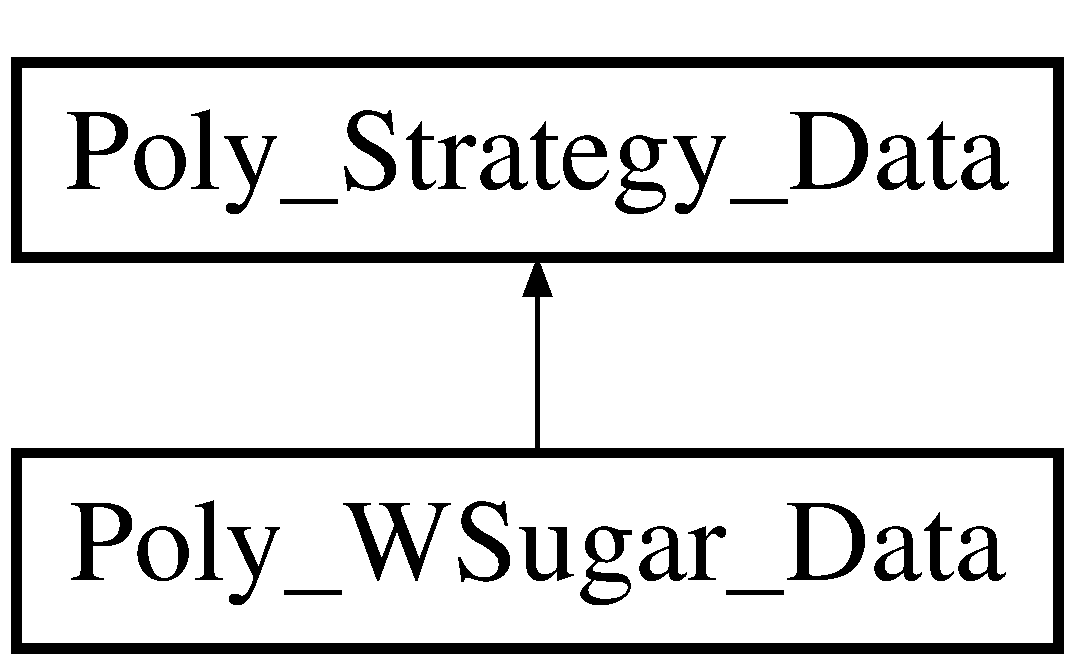
\includegraphics[height=2.000000cm]{group__strategygroup}
\end{center}
\end{figure}
\subsubsection*{Public Member Functions}
\begin{Indent}\textbf{ Destruction}\par
\begin{DoxyCompactItemize}
\item 
\mbox{\Hypertarget{group__strategygroup_a177d4749902d7c94d8e48340a64d87b7}\label{group__strategygroup_a177d4749902d7c94d8e48340a64d87b7}} 
virtual {\bfseries $\sim$\+Pair\+\_\+\+Strategy\+\_\+\+Data} ()
\end{DoxyCompactItemize}
\end{Indent}
\begin{Indent}\textbf{ Comparison}\par
\begin{DoxyCompactItemize}
\item 
\mbox{\Hypertarget{group__strategygroup_ae29822eaf584f1f9654c4ec821734279}\label{group__strategygroup_ae29822eaf584f1f9654c4ec821734279}} 
virtual bool \hyperlink{group__strategygroup_ae29822eaf584f1f9654c4ec821734279}{equivalent} (const \hyperlink{group__strategygroup_class_pair___strategy___data}{Pair\+\_\+\+Strategy\+\_\+\+Data} \&) const =0
\begin{DoxyCompactList}\small\item\em should return {\ttfamily true} iff {\ttfamily this} and other are equivalent \end{DoxyCompactList}\item 
\mbox{\Hypertarget{group__strategygroup_a41f03829d564520427fb9405aefe41be}\label{group__strategygroup_a41f03829d564520427fb9405aefe41be}} 
bool \hyperlink{group__strategygroup_a41f03829d564520427fb9405aefe41be}{operator==} (const \hyperlink{group__strategygroup_class_pair___strategy___data}{Pair\+\_\+\+Strategy\+\_\+\+Data} \&sd) const
\begin{DoxyCompactList}\small\item\em alias for \hyperlink{group__strategygroup_ae29822eaf584f1f9654c4ec821734279}{equivalent()} \end{DoxyCompactList}\item 
\mbox{\Hypertarget{group__strategygroup_a272edeb1893af886b4449d7bcb799cdb}\label{group__strategygroup_a272edeb1893af886b4449d7bcb799cdb}} 
virtual bool \hyperlink{group__strategygroup_a272edeb1893af886b4449d7bcb799cdb}{first\+\_\+larger} (const \hyperlink{group__strategygroup_class_pair___strategy___data}{Pair\+\_\+\+Strategy\+\_\+\+Data} \&) const =0
\begin{DoxyCompactList}\small\item\em should return {\ttfamily true} iff {\ttfamily this} is larger than other \end{DoxyCompactList}\item 
\mbox{\Hypertarget{group__strategygroup_aed30bba9721f2497fc80393ca2d26930}\label{group__strategygroup_aed30bba9721f2497fc80393ca2d26930}} 
bool \hyperlink{group__strategygroup_aed30bba9721f2497fc80393ca2d26930}{operator$>$} (const \hyperlink{group__strategygroup_class_pair___strategy___data}{Pair\+\_\+\+Strategy\+\_\+\+Data} \&sd) const
\begin{DoxyCompactList}\small\item\em alias for \hyperlink{group__strategygroup_a272edeb1893af886b4449d7bcb799cdb}{first\+\_\+larger()} \end{DoxyCompactList}\item 
\mbox{\Hypertarget{group__strategygroup_ac72e2a5cef6f9a6dafdb82f97495fd8b}\label{group__strategygroup_ac72e2a5cef6f9a6dafdb82f97495fd8b}} 
bool \hyperlink{group__strategygroup_ac72e2a5cef6f9a6dafdb82f97495fd8b}{operator$>$=} (const \hyperlink{group__strategygroup_class_pair___strategy___data}{Pair\+\_\+\+Strategy\+\_\+\+Data} \&sd) const
\begin{DoxyCompactList}\small\item\em is {\ttfamily this} larger than or equivalent to other? \end{DoxyCompactList}\item 
\mbox{\Hypertarget{group__strategygroup_a5d5459ea25db09d848ab616c395fc209}\label{group__strategygroup_a5d5459ea25db09d848ab616c395fc209}} 
bool \hyperlink{group__strategygroup_a5d5459ea25db09d848ab616c395fc209}{operator$<$} (const \hyperlink{group__strategygroup_class_pair___strategy___data}{Pair\+\_\+\+Strategy\+\_\+\+Data} \&sd) const
\begin{DoxyCompactList}\small\item\em is {\ttfamily this} smaller than other? \end{DoxyCompactList}\item 
\mbox{\Hypertarget{group__strategygroup_a19030cdc7b1f92c5941a78276e298f67}\label{group__strategygroup_a19030cdc7b1f92c5941a78276e298f67}} 
bool \hyperlink{group__strategygroup_a19030cdc7b1f92c5941a78276e298f67}{operator$<$=} (const \hyperlink{group__strategygroup_class_pair___strategy___data}{Pair\+\_\+\+Strategy\+\_\+\+Data} \&sd) const
\begin{DoxyCompactList}\small\item\em is {\ttfamily this} smaller than or equivalent to other? \end{DoxyCompactList}\end{DoxyCompactItemize}
\end{Indent}
\begin{Indent}\textbf{ Computation}\par
\begin{DoxyCompactItemize}
\item 
virtual void \hyperlink{group__strategygroup_a15fdaa9fa3cc0a259e7dd29df1940819}{pre\+\_\+spolynomial\+\_\+tasks} () const
\begin{DoxyCompactList}\small\item\em hook called immediately before computing a new s-\/polynomiald \end{DoxyCompactList}\end{DoxyCompactItemize}
\end{Indent}


\paragraph{Member Function Documentation}
\mbox{\Hypertarget{group__strategygroup_a15fdaa9fa3cc0a259e7dd29df1940819}\label{group__strategygroup_a15fdaa9fa3cc0a259e7dd29df1940819}} 
\index{Pair\+\_\+\+Strategy\+\_\+\+Data@{Pair\+\_\+\+Strategy\+\_\+\+Data}!pre\+\_\+spolynomial\+\_\+tasks@{pre\+\_\+spolynomial\+\_\+tasks}}
\index{pre\+\_\+spolynomial\+\_\+tasks@{pre\+\_\+spolynomial\+\_\+tasks}!Pair\+\_\+\+Strategy\+\_\+\+Data@{Pair\+\_\+\+Strategy\+\_\+\+Data}}
\subparagraph{\texorpdfstring{pre\+\_\+spolynomial\+\_\+tasks()}{pre\_spolynomial\_tasks()}}
{\footnotesize\ttfamily void Pair\+\_\+\+Strategy\+\_\+\+Data\+::pre\+\_\+spolynomial\+\_\+tasks (\begin{DoxyParamCaption}{ }\end{DoxyParamCaption}) const\hspace{0.3cm}{\ttfamily [virtual]}}



hook called immediately before computing a new s-\/polynomiald 

The default is to do nothing, which is good for the normal strategy. Other strategies, however, may require some processing before reduction; the sugar strategy is an example, as an s-\/polynomial needs to record a new polynomial's sugar 

Definition at line 74 of file strategies.\+cpp.

\index{Pair\+\_\+\+Sugar\+\_\+\+Data@{Pair\+\_\+\+Sugar\+\_\+\+Data}}\label{class_pair___sugar___data}
\Hypertarget{group__strategygroup_class_pair___sugar___data}
\subsubsection{class Pair\+\_\+\+Sugar\+\_\+\+Data}
ordering critical pairs using the sugar strategy 

\begin{DoxyAuthor}{Author}
John Perry 
\end{DoxyAuthor}
\begin{DoxyDate}{Date}
2016 
\end{DoxyDate}


Definition at line 101 of file sugar\+\_\+strategy.\+hpp.

Inheritance diagram for Pair\+\_\+\+Sugar\+\_\+\+Data\+:\begin{figure}[H]
\begin{center}
\leavevmode
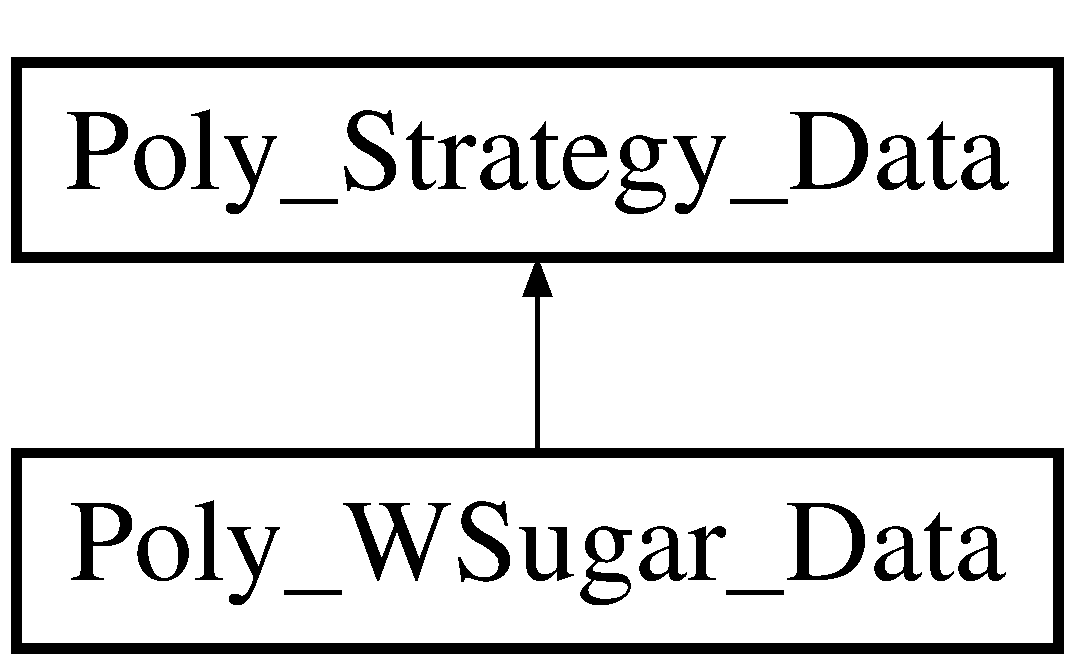
\includegraphics[height=2.000000cm]{group__strategygroup}
\end{center}
\end{figure}
\subsubsection*{Public Member Functions}
\begin{Indent}\textbf{ Construction}\par
\begin{DoxyCompactItemize}
\item 
\mbox{\Hypertarget{group__strategygroup_a2f244064c356cd5c33164adf75177fac}\label{group__strategygroup_a2f244064c356cd5c33164adf75177fac}} 
\hyperlink{group__strategygroup_a2f244064c356cd5c33164adf75177fac}{Pair\+\_\+\+Sugar\+\_\+\+Data} (\hyperlink{group___g_b_computation_class_critical___pair___basic}{Critical\+\_\+\+Pair\+\_\+\+Basic} \&cpb)
\begin{DoxyCompactList}\small\item\em all the information we need is in {\ttfamily cpb} already so no additional processing is necessary \end{DoxyCompactList}\end{DoxyCompactItemize}
\end{Indent}
\begin{Indent}\textbf{ Comparison}\par
\begin{DoxyCompactItemize}
\item 
\mbox{\Hypertarget{group__strategygroup_abd2ef27e308ee646a64b448ad63e941b}\label{group__strategygroup_abd2ef27e308ee646a64b448ad63e941b}} 
virtual bool \hyperlink{group__strategygroup_abd2ef27e308ee646a64b448ad63e941b}{equivalent} (const \hyperlink{group__strategygroup_class_pair___strategy___data}{Pair\+\_\+\+Strategy\+\_\+\+Data} \&sd) const
\begin{DoxyCompactList}\small\item\em implementation of \hyperlink{group__strategygroup_abd2ef27e308ee646a64b448ad63e941b}{equivalent()} \end{DoxyCompactList}\item 
\mbox{\Hypertarget{group__strategygroup_aa898723612943072f6b83eaaa58b70ce}\label{group__strategygroup_aa898723612943072f6b83eaaa58b70ce}} 
virtual bool \hyperlink{group__strategygroup_aa898723612943072f6b83eaaa58b70ce}{first\+\_\+larger} (const \hyperlink{group__strategygroup_class_pair___strategy___data}{Pair\+\_\+\+Strategy\+\_\+\+Data} \&sd) const
\begin{DoxyCompactList}\small\item\em implementation of \hyperlink{group__strategygroup_aa898723612943072f6b83eaaa58b70ce}{first\+\_\+larger()} \end{DoxyCompactList}\end{DoxyCompactItemize}
\end{Indent}
\begin{Indent}\textbf{ Basic properties}\par
\begin{DoxyCompactItemize}
\item 
\mbox{\Hypertarget{group__strategygroup_af2fddc7e7baf0b270ce9789e4dee5290}\label{group__strategygroup_af2fddc7e7baf0b270ce9789e4dee5290}} 
D\+E\+G\+\_\+\+T\+Y\+PE {\bfseries pair\+\_\+sugar} () const
\end{DoxyCompactItemize}
\end{Indent}
\subsubsection*{Protected Attributes}
\begin{DoxyCompactItemize}
\item 
\mbox{\Hypertarget{group__strategygroup_a296c0a6eb2e16d5b7628ccf3df8f29c6}\label{group__strategygroup_a296c0a6eb2e16d5b7628ccf3df8f29c6}} 
\hyperlink{group___g_b_computation_class_critical___pair___basic}{Critical\+\_\+\+Pair\+\_\+\+Basic} $\ast$ \hyperlink{group__strategygroup_a296c0a6eb2e16d5b7628ccf3df8f29c6}{cp}
\begin{DoxyCompactList}\small\item\em the critical pair to which this {\ttfamily \hyperlink{group__strategygroup_class_normal___strategy}{Normal\+\_\+\+Strategy}} belongs \end{DoxyCompactList}\item 
\mbox{\Hypertarget{group__strategygroup_a8d743628b73ac3f4de3df1ec306263bb}\label{group__strategygroup_a8d743628b73ac3f4de3df1ec306263bb}} 
D\+E\+G\+\_\+\+T\+Y\+PE \hyperlink{group__strategygroup_a8d743628b73ac3f4de3df1ec306263bb}{sugar}
\begin{DoxyCompactList}\small\item\em the pair$\ast$rsquo;s sugar \end{DoxyCompactList}\end{DoxyCompactItemize}
\index{Pair\+\_\+\+W\+Sugar\+\_\+\+Strategy@{Pair\+\_\+\+W\+Sugar\+\_\+\+Strategy}}\label{class_pair___w_sugar___strategy}
\Hypertarget{group__strategygroup_class_pair___w_sugar___strategy}
\subsubsection{class Pair\+\_\+\+W\+Sugar\+\_\+\+Strategy}
ordering critical pairs using the weighted sugar strategy 

\begin{DoxyAuthor}{Author}
John Perry 
\end{DoxyAuthor}
\begin{DoxyDate}{Date}
2016 
\end{DoxyDate}


Definition at line 116 of file weighted\+\_\+sugar\+\_\+strategy.\+hpp.

Inheritance diagram for Pair\+\_\+\+W\+Sugar\+\_\+\+Strategy\+:\begin{figure}[H]
\begin{center}
\leavevmode
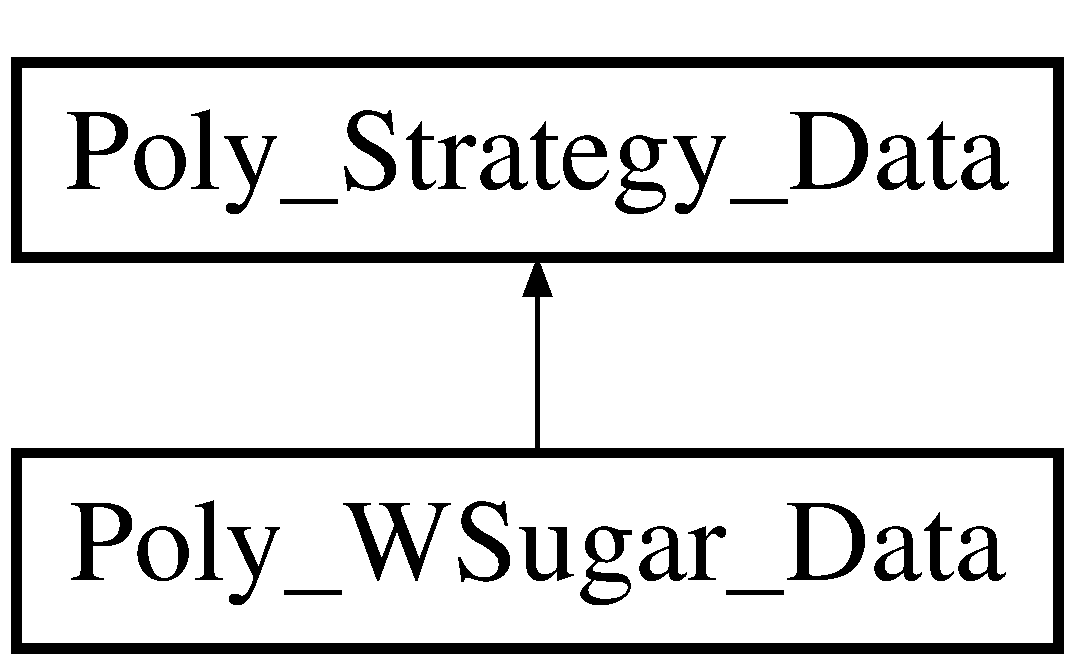
\includegraphics[height=2.000000cm]{group__strategygroup}
\end{center}
\end{figure}
\subsubsection*{Public Member Functions}
\begin{Indent}\textbf{ Construction}\par
\begin{DoxyCompactItemize}
\item 
\mbox{\Hypertarget{group__strategygroup_af06bcaf5995724fe80283e20f91151b1}\label{group__strategygroup_af06bcaf5995724fe80283e20f91151b1}} 
\hyperlink{group__strategygroup_af06bcaf5995724fe80283e20f91151b1}{Pair\+\_\+\+W\+Sugar\+\_\+\+Strategy} (\hyperlink{group___g_b_computation_class_critical___pair___basic}{Critical\+\_\+\+Pair\+\_\+\+Basic} \&)
\begin{DoxyCompactList}\small\item\em creates a pair whose weighted sugar is the maximum of that of the products of the polynomials in the critical pair \end{DoxyCompactList}\end{DoxyCompactItemize}
\end{Indent}
\begin{Indent}\textbf{ Comparison}\par
\begin{DoxyCompactItemize}
\item 
\mbox{\Hypertarget{group__strategygroup_a6a46188917beeab6617ff27d70356860}\label{group__strategygroup_a6a46188917beeab6617ff27d70356860}} 
virtual bool \hyperlink{group__strategygroup_a6a46188917beeab6617ff27d70356860}{equivalent} (const \hyperlink{group__strategygroup_class_pair___strategy___data}{Pair\+\_\+\+Strategy\+\_\+\+Data} \&sd) const
\begin{DoxyCompactList}\small\item\em implementation of \hyperlink{group__strategygroup_a6a46188917beeab6617ff27d70356860}{equivalent()} \end{DoxyCompactList}\item 
\mbox{\Hypertarget{group__strategygroup_afe1c908cbb040ee318bed323395c0441}\label{group__strategygroup_afe1c908cbb040ee318bed323395c0441}} 
virtual bool \hyperlink{group__strategygroup_afe1c908cbb040ee318bed323395c0441}{first\+\_\+larger} (const \hyperlink{group__strategygroup_class_pair___strategy___data}{Pair\+\_\+\+Strategy\+\_\+\+Data} \&sd) const
\begin{DoxyCompactList}\small\item\em implementation of \hyperlink{group__strategygroup_afe1c908cbb040ee318bed323395c0441}{first\+\_\+larger()} \end{DoxyCompactList}\end{DoxyCompactItemize}
\end{Indent}
\begin{Indent}\textbf{ Basic properties}\par
\begin{DoxyCompactItemize}
\item 
\mbox{\Hypertarget{group__strategygroup_abaf1d3aa2eb6b7fef429be8f27e2c7b8}\label{group__strategygroup_abaf1d3aa2eb6b7fef429be8f27e2c7b8}} 
D\+E\+G\+\_\+\+T\+Y\+PE \hyperlink{group__strategygroup_abaf1d3aa2eb6b7fef429be8f27e2c7b8}{pair\+\_\+sugar} ()
\begin{DoxyCompactList}\small\item\em the weighted sugar \end{DoxyCompactList}\end{DoxyCompactItemize}
\end{Indent}
\begin{Indent}\textbf{ Modification}\par
{\em Useful for when the ordering changes. }\begin{DoxyCompactItemize}
\item 
\mbox{\Hypertarget{group__strategygroup_a5288aef295d144401e9c0a7c08c40a66}\label{group__strategygroup_a5288aef295d144401e9c0a7c08c40a66}} 
virtual void {\bfseries adjust\+\_\+sugar} (D\+E\+G\+\_\+\+T\+Y\+PE new\+\_\+sugar)
\end{DoxyCompactItemize}
\end{Indent}
\subsubsection*{Protected Attributes}
\begin{DoxyCompactItemize}
\item 
\mbox{\Hypertarget{group__strategygroup_ad64f04d4feffa02e64ff4837b55a7def}\label{group__strategygroup_ad64f04d4feffa02e64ff4837b55a7def}} 
\hyperlink{group___g_b_computation_class_critical___pair___basic}{Critical\+\_\+\+Pair\+\_\+\+Basic} $\ast$ \hyperlink{group__strategygroup_ad64f04d4feffa02e64ff4837b55a7def}{cp}
\begin{DoxyCompactList}\small\item\em the critical pair to which this {\ttfamily \hyperlink{group__strategygroup_class_normal___strategy}{Normal\+\_\+\+Strategy}} belongs \end{DoxyCompactList}\item 
\mbox{\Hypertarget{group__strategygroup_a6bd5a8eb9113fd93475c06e30da44bb8}\label{group__strategygroup_a6bd5a8eb9113fd93475c06e30da44bb8}} 
D\+E\+G\+\_\+\+T\+Y\+PE \hyperlink{group__strategygroup_a6bd5a8eb9113fd93475c06e30da44bb8}{sugar}
\begin{DoxyCompactList}\small\item\em the pair$\ast$rsquo;s sugar \end{DoxyCompactList}\end{DoxyCompactItemize}
\index{Poly\+\_\+\+Strategy\+\_\+\+Data@{Poly\+\_\+\+Strategy\+\_\+\+Data}}\label{class_poly___strategy___data}
\Hypertarget{group__strategygroup_class_poly___strategy___data}
\subsubsection{class Poly\+\_\+\+Strategy\+\_\+\+Data}
polynomial-\/related strategy data 

\begin{DoxyAuthor}{Author}
John Perry 
\end{DoxyAuthor}
\begin{DoxyDate}{Date}
2016
\end{DoxyDate}
Some strategies will not need this class, but others will, such as sugar (to store a polynomial's sugar). 

Definition at line 49 of file strategies.\+hpp.

Inheritance diagram for Poly\+\_\+\+Strategy\+\_\+\+Data\+:\begin{figure}[H]
\begin{center}
\leavevmode
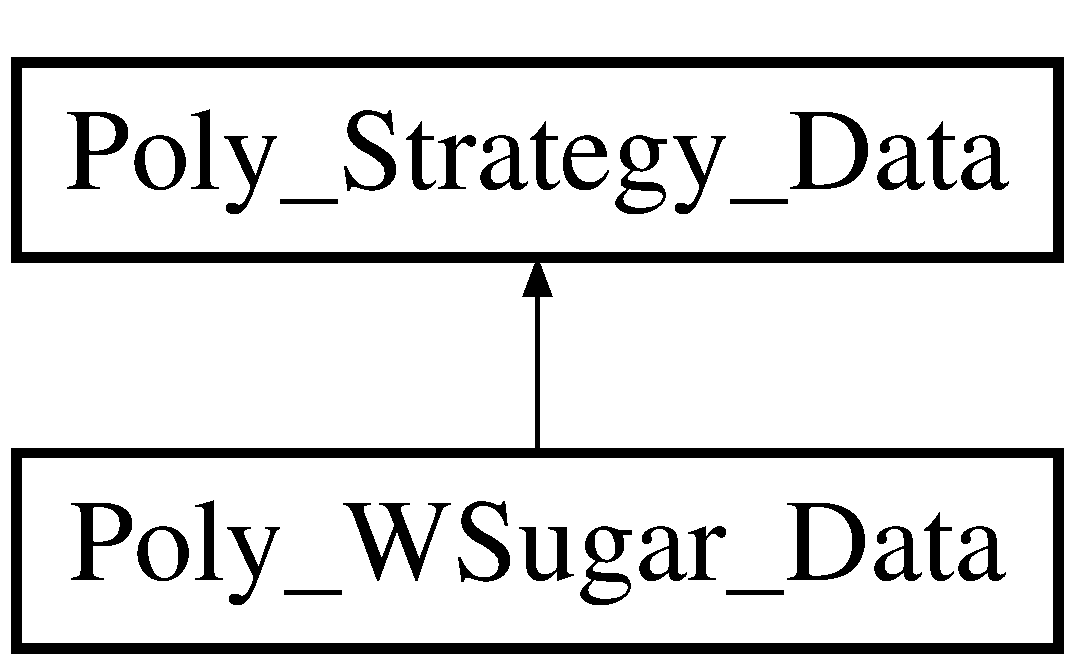
\includegraphics[height=2.000000cm]{group__strategygroup}
\end{center}
\end{figure}
\subsubsection*{Public Member Functions}
\begin{Indent}\textbf{ Destruction}\par
\begin{DoxyCompactItemize}
\item 
\mbox{\Hypertarget{group__strategygroup_acdbc88a35a960f6f2934947de32b1f20}\label{group__strategygroup_acdbc88a35a960f6f2934947de32b1f20}} 
virtual {\bfseries $\sim$\+Poly\+\_\+\+Strategy\+\_\+\+Data} ()
\end{DoxyCompactItemize}
\end{Indent}
\begin{Indent}\textbf{ Basic properties}\par
\begin{DoxyCompactItemize}
\item 
\mbox{\Hypertarget{group__strategygroup_a305ffff282203eaccd7f1709634bc5d4}\label{group__strategygroup_a305ffff282203eaccd7f1709634bc5d4}} 
virtual \hyperlink{group__strategygroup_ga0ee6c8e033547330e6b89929730007f4}{Strategy\+Flags} {\bfseries type} ()=0
\end{DoxyCompactItemize}
\end{Indent}
\begin{Indent}\textbf{ Comparison}\par
\begin{DoxyCompactItemize}
\item 
\mbox{\Hypertarget{group__strategygroup_aa82a57a8bf9b3c14fd65a573fd78a4a5}\label{group__strategygroup_aa82a57a8bf9b3c14fd65a573fd78a4a5}} 
virtual bool \hyperlink{group__strategygroup_aa82a57a8bf9b3c14fd65a573fd78a4a5}{equivalent} (const \hyperlink{group__strategygroup_class_poly___strategy___data}{Poly\+\_\+\+Strategy\+\_\+\+Data} \&) const =0
\begin{DoxyCompactList}\small\item\em should return {\ttfamily true} iff strategy considers {\ttfamily this} and other equivalent \end{DoxyCompactList}\item 
\mbox{\Hypertarget{group__strategygroup_a5c88b8a0a17d4175bf43ccab5d7ded4f}\label{group__strategygroup_a5c88b8a0a17d4175bf43ccab5d7ded4f}} 
bool \hyperlink{group__strategygroup_a5c88b8a0a17d4175bf43ccab5d7ded4f}{operator==} (const \hyperlink{group__strategygroup_class_poly___strategy___data}{Poly\+\_\+\+Strategy\+\_\+\+Data} \&other) const
\begin{DoxyCompactList}\small\item\em alias for \hyperlink{group__strategygroup_aa82a57a8bf9b3c14fd65a573fd78a4a5}{equivalent()} \end{DoxyCompactList}\item 
\mbox{\Hypertarget{group__strategygroup_a6cd4608015a6b0f06141b9b73b0d4137}\label{group__strategygroup_a6cd4608015a6b0f06141b9b73b0d4137}} 
virtual bool \hyperlink{group__strategygroup_a6cd4608015a6b0f06141b9b73b0d4137}{first\+\_\+larger} (const \hyperlink{group__strategygroup_class_poly___strategy___data}{Poly\+\_\+\+Strategy\+\_\+\+Data} \&) const =0
\begin{DoxyCompactList}\small\item\em should return {\ttfamily true} iff strategy considers {\ttfamily this} larger than other \end{DoxyCompactList}\item 
\mbox{\Hypertarget{group__strategygroup_a4100b95343145b454dca2978545dd791}\label{group__strategygroup_a4100b95343145b454dca2978545dd791}} 
bool \hyperlink{group__strategygroup_a4100b95343145b454dca2978545dd791}{operator$>$} (const \hyperlink{group__strategygroup_class_poly___strategy___data}{Poly\+\_\+\+Strategy\+\_\+\+Data} \&other) const
\begin{DoxyCompactList}\small\item\em alias for \hyperlink{group__strategygroup_a6cd4608015a6b0f06141b9b73b0d4137}{first\+\_\+larger()} \end{DoxyCompactList}\item 
\mbox{\Hypertarget{group__strategygroup_a10eaa72d8dd9d02be47c7450d0358911}\label{group__strategygroup_a10eaa72d8dd9d02be47c7450d0358911}} 
bool \hyperlink{group__strategygroup_a10eaa72d8dd9d02be47c7450d0358911}{operator$>$=} (const \hyperlink{group__strategygroup_class_poly___strategy___data}{Poly\+\_\+\+Strategy\+\_\+\+Data} \&other) const
\begin{DoxyCompactList}\small\item\em is {\ttfamily this} larger than or equivalent to other? \end{DoxyCompactList}\item 
\mbox{\Hypertarget{group__strategygroup_a77f188486ec685a0848eb8ff21d9c1cc}\label{group__strategygroup_a77f188486ec685a0848eb8ff21d9c1cc}} 
bool \hyperlink{group__strategygroup_a77f188486ec685a0848eb8ff21d9c1cc}{operator$<$} (const \hyperlink{group__strategygroup_class_poly___strategy___data}{Poly\+\_\+\+Strategy\+\_\+\+Data} \&other) const
\begin{DoxyCompactList}\small\item\em is {\ttfamily this} smaller than other? \end{DoxyCompactList}\item 
\mbox{\Hypertarget{group__strategygroup_a861774f75e0585613a250483728a7ed2}\label{group__strategygroup_a861774f75e0585613a250483728a7ed2}} 
bool \hyperlink{group__strategygroup_a861774f75e0585613a250483728a7ed2}{operator$<$=} (const \hyperlink{group__strategygroup_class_poly___strategy___data}{Poly\+\_\+\+Strategy\+\_\+\+Data} \&other) const
\begin{DoxyCompactList}\small\item\em is {\ttfamily this} smaller than or equivalent to other? \end{DoxyCompactList}\end{DoxyCompactItemize}
\end{Indent}
\begin{Indent}\textbf{ Computation}\par
\begin{DoxyCompactItemize}
\item 
virtual void \hyperlink{group__strategygroup_a3c2e31f0e3323da59564edc6ee3557af}{at\+\_\+generation\+\_\+tasks} ()
\begin{DoxyCompactList}\small\item\em hook called while first generating polynomial \end{DoxyCompactList}\item 
virtual void \hyperlink{group__strategygroup_a6683749a5fb30b6f91075a28899fbfe7}{at\+\_\+generation\+\_\+tasks} (const \hyperlink{group__polygroup_class_monomial}{Monomial} \&t)
\begin{DoxyCompactList}\small\item\em hook called while first generating a polynomial {\itshape multiple} \end{DoxyCompactList}\item 
virtual bool \hyperlink{group__strategygroup_a996754ff163b0ff32d783ec723ac35be}{valid\+\_\+reduction} (const \hyperlink{group__polygroup_class_abstract___polynomial}{Abstract\+\_\+\+Polynomial} \&r, const \hyperlink{group__polygroup_class_abstract___polynomial}{Abstract\+\_\+\+Polynomial} \&g) const
\begin{DoxyCompactList}\small\item\em hook called while finding a reducer \end{DoxyCompactList}\item 
\mbox{\Hypertarget{group__strategygroup_a27fb1565f1c569ca28f01021551a1353}\label{group__strategygroup_a27fb1565f1c569ca28f01021551a1353}} 
void {\bfseries pre\+\_\+reduction\+\_\+tasks} (const \hyperlink{group__polygroup_class_monomial}{Monomial} \&u, const \hyperlink{group__polygroup_class_abstract___polynomial}{Abstract\+\_\+\+Polynomial} \&g)
\item 
virtual void \hyperlink{group__strategygroup_a0d71db50c58a24f48f94eae6a48c2149}{pre\+\_\+reduction\+\_\+tasks} (const E\+X\+P\+\_\+\+T\+Y\+PE $\ast$u, const \hyperlink{group__polygroup_class_abstract___polynomial}{Abstract\+\_\+\+Polynomial} \&g)
\begin{DoxyCompactList}\small\item\em hook called immediately before performing reduction \end{DoxyCompactList}\end{DoxyCompactItemize}
\end{Indent}
\subsubsection*{Protected Attributes}
\begin{DoxyCompactItemize}
\item 
\mbox{\Hypertarget{group__strategygroup_a2fdcdbe5f8ea3ae93c5a55a9775e6e6f}\label{group__strategygroup_a2fdcdbe5f8ea3ae93c5a55a9775e6e6f}} 
const \hyperlink{group__polygroup_class_abstract___polynomial}{Abstract\+\_\+\+Polynomial} $\ast$ \hyperlink{group__strategygroup_a2fdcdbe5f8ea3ae93c5a55a9775e6e6f}{p}
\begin{DoxyCompactList}\small\item\em the polynomial to which this strategy applies \end{DoxyCompactList}\end{DoxyCompactItemize}
\subsubsection*{Friends}
\begin{Indent}\textbf{ I/O}\par
\begin{DoxyCompactItemize}
\item 
\mbox{\Hypertarget{group__strategygroup_a10f553f550739a68fe90fa3318942134}\label{group__strategygroup_a10f553f550739a68fe90fa3318942134}} 
ostream \& \hyperlink{group__strategygroup_a10f553f550739a68fe90fa3318942134}{operator$<$$<$} (ostream \&, const \hyperlink{group__strategygroup_class_poly___strategy___data}{Poly\+\_\+\+Strategy\+\_\+\+Data} \&)
\begin{DoxyCompactList}\small\item\em print strategy-\/related data in the polynomial \end{DoxyCompactList}\end{DoxyCompactItemize}
\end{Indent}


\paragraph{Member Function Documentation}
\mbox{\Hypertarget{group__strategygroup_a3c2e31f0e3323da59564edc6ee3557af}\label{group__strategygroup_a3c2e31f0e3323da59564edc6ee3557af}} 
\index{Poly\+\_\+\+Strategy\+\_\+\+Data@{Poly\+\_\+\+Strategy\+\_\+\+Data}!at\+\_\+generation\+\_\+tasks@{at\+\_\+generation\+\_\+tasks}}
\index{at\+\_\+generation\+\_\+tasks@{at\+\_\+generation\+\_\+tasks}!Poly\+\_\+\+Strategy\+\_\+\+Data@{Poly\+\_\+\+Strategy\+\_\+\+Data}}
\subparagraph{\texorpdfstring{at\+\_\+generation\+\_\+tasks()}{at\_generation\_tasks()}\hspace{0.1cm}{\footnotesize\ttfamily [1/2]}}
{\footnotesize\ttfamily virtual void Poly\+\_\+\+Strategy\+\_\+\+Data\+::at\+\_\+generation\+\_\+tasks (\begin{DoxyParamCaption}{ }\end{DoxyParamCaption})\hspace{0.3cm}{\ttfamily [inline]}, {\ttfamily [virtual]}}



hook called while first generating polynomial 

The default is to do nothing, which is good for the normal strategy. Other strategies, however, may perform some record-\/keeping; the sugar strategy, for instance, will compute the polynomial's sugar. 

Reimplemented in \hyperlink{group__strategygroup_ac07ee9ee15bd97e5e8befb3f6cec3929}{Poly\+\_\+\+W\+Sugar\+\_\+\+Data}, and \hyperlink{group__strategygroup_ada533e5c56d7f53207a5e8093414dfb3}{Poly\+\_\+\+Sugar\+\_\+\+Data}.



Definition at line 88 of file strategies.\+hpp.

\mbox{\Hypertarget{group__strategygroup_a6683749a5fb30b6f91075a28899fbfe7}\label{group__strategygroup_a6683749a5fb30b6f91075a28899fbfe7}} 
\index{Poly\+\_\+\+Strategy\+\_\+\+Data@{Poly\+\_\+\+Strategy\+\_\+\+Data}!at\+\_\+generation\+\_\+tasks@{at\+\_\+generation\+\_\+tasks}}
\index{at\+\_\+generation\+\_\+tasks@{at\+\_\+generation\+\_\+tasks}!Poly\+\_\+\+Strategy\+\_\+\+Data@{Poly\+\_\+\+Strategy\+\_\+\+Data}}
\subparagraph{\texorpdfstring{at\+\_\+generation\+\_\+tasks()}{at\_generation\_tasks()}\hspace{0.1cm}{\footnotesize\ttfamily [2/2]}}
{\footnotesize\ttfamily virtual void Poly\+\_\+\+Strategy\+\_\+\+Data\+::at\+\_\+generation\+\_\+tasks (\begin{DoxyParamCaption}\item[{const \hyperlink{group__polygroup_class_monomial}{Monomial} \&}]{t }\end{DoxyParamCaption})\hspace{0.3cm}{\ttfamily [inline]}, {\ttfamily [virtual]}}



hook called while first generating a polynomial {\itshape multiple} 


\begin{DoxyParams}{Parameters}
{\em t} & a \hyperlink{group__polygroup_class_monomial}{Monomial} that we are about to multiply to create an s-\/polynomial\\
\hline
\end{DoxyParams}
The default is to do nothing, which is good for the normal strategy. Other strategies, however, may perform some record-\/keeping; the sugar strategy, for instance, will compute the polynomial's sugar. 

Reimplemented in \hyperlink{group__strategygroup_ac58bd8d30e7e10dbbe8e86b1d9d04376}{Poly\+\_\+\+W\+Sugar\+\_\+\+Data}, and \hyperlink{group__strategygroup_aa80c660f10b1c5d0dd2a305d598685f5}{Poly\+\_\+\+Sugar\+\_\+\+Data}.



Definition at line 96 of file strategies.\+hpp.

\mbox{\Hypertarget{group__strategygroup_a0d71db50c58a24f48f94eae6a48c2149}\label{group__strategygroup_a0d71db50c58a24f48f94eae6a48c2149}} 
\index{Poly\+\_\+\+Strategy\+\_\+\+Data@{Poly\+\_\+\+Strategy\+\_\+\+Data}!pre\+\_\+reduction\+\_\+tasks@{pre\+\_\+reduction\+\_\+tasks}}
\index{pre\+\_\+reduction\+\_\+tasks@{pre\+\_\+reduction\+\_\+tasks}!Poly\+\_\+\+Strategy\+\_\+\+Data@{Poly\+\_\+\+Strategy\+\_\+\+Data}}
\subparagraph{\texorpdfstring{pre\+\_\+reduction\+\_\+tasks()}{pre\_reduction\_tasks()}}
{\footnotesize\ttfamily virtual void Poly\+\_\+\+Strategy\+\_\+\+Data\+::pre\+\_\+reduction\+\_\+tasks (\begin{DoxyParamCaption}\item[{const E\+X\+P\+\_\+\+T\+Y\+PE $\ast$}]{u,  }\item[{const \hyperlink{group__polygroup_class_abstract___polynomial}{Abstract\+\_\+\+Polynomial} \&}]{g }\end{DoxyParamCaption})\hspace{0.3cm}{\ttfamily [inline]}, {\ttfamily [virtual]}}



hook called immediately before performing reduction 


\begin{DoxyParams}{Parameters}
{\em g} & polynomial that reduces {\ttfamily r} (where {\ttfamily r} is {\ttfamily this}) \\
\hline
{\em u} & exponents of monomial satisfying $u\textrm{lm}(g)=\textrm{lm}(r)$\\
\hline
\end{DoxyParams}
The default is to do nothing, which is good for the normal strategy. Other strategies, however, may require some processing before reduction; the sugar strategy is an example, as reduction may increase a polynomial's sugar 

Reimplemented in \hyperlink{group__strategygroup_a4a34039eb50a2294d2aaf6245c1833b8}{Poly\+\_\+\+W\+Sugar\+\_\+\+Data}, and \hyperlink{group__strategygroup_a1b2e8a7fe4fcd57555fa58e48620b2bf}{Poly\+\_\+\+Sugar\+\_\+\+Data}.



Definition at line 124 of file strategies.\+hpp.

\mbox{\Hypertarget{group__strategygroup_a996754ff163b0ff32d783ec723ac35be}\label{group__strategygroup_a996754ff163b0ff32d783ec723ac35be}} 
\index{Poly\+\_\+\+Strategy\+\_\+\+Data@{Poly\+\_\+\+Strategy\+\_\+\+Data}!valid\+\_\+reduction@{valid\+\_\+reduction}}
\index{valid\+\_\+reduction@{valid\+\_\+reduction}!Poly\+\_\+\+Strategy\+\_\+\+Data@{Poly\+\_\+\+Strategy\+\_\+\+Data}}
\subparagraph{\texorpdfstring{valid\+\_\+reduction()}{valid\_reduction()}}
{\footnotesize\ttfamily bool Poly\+\_\+\+Strategy\+\_\+\+Data\+::valid\+\_\+reduction (\begin{DoxyParamCaption}\item[{const \hyperlink{group__polygroup_class_abstract___polynomial}{Abstract\+\_\+\+Polynomial} \&}]{r,  }\item[{const \hyperlink{group__polygroup_class_abstract___polynomial}{Abstract\+\_\+\+Polynomial} \&}]{g }\end{DoxyParamCaption}) const\hspace{0.3cm}{\ttfamily [virtual]}}



hook called while finding a reducer 


\begin{DoxyParams}{Parameters}
{\em r} & polynomial that is to be reduced \\
\hline
{\em g} & polynomial that reduces {\ttfamily r} \\
\hline
\end{DoxyParams}
\begin{DoxyReturn}{Returns}
{\ttfamily true} if and only if it is valid to reduce {\ttfamily r} by {\ttfamily g} 
\end{DoxyReturn}
The default is to do nothing, which is good for the normal and sugar strategies. Other strategies, however, may impose constraints on the reduction; involutive and signature-\/based reduction, for instance, both forbid certain reductions. 

Definition at line 43 of file strategies.\+cpp.

\index{Poly\+\_\+\+Sugar\+\_\+\+Data@{Poly\+\_\+\+Sugar\+\_\+\+Data}}\label{class_poly___sugar___data}
\Hypertarget{group__strategygroup_class_poly___sugar___data}
\subsubsection{class Poly\+\_\+\+Sugar\+\_\+\+Data}
polynomial-\/related data for a sugar strategy 

\begin{DoxyAuthor}{Author}
John Perry 
\end{DoxyAuthor}
\begin{DoxyDate}{Date}
2016 
\end{DoxyDate}


Definition at line 33 of file sugar\+\_\+strategy.\+hpp.

Inheritance diagram for Poly\+\_\+\+Sugar\+\_\+\+Data\+:\begin{figure}[H]
\begin{center}
\leavevmode
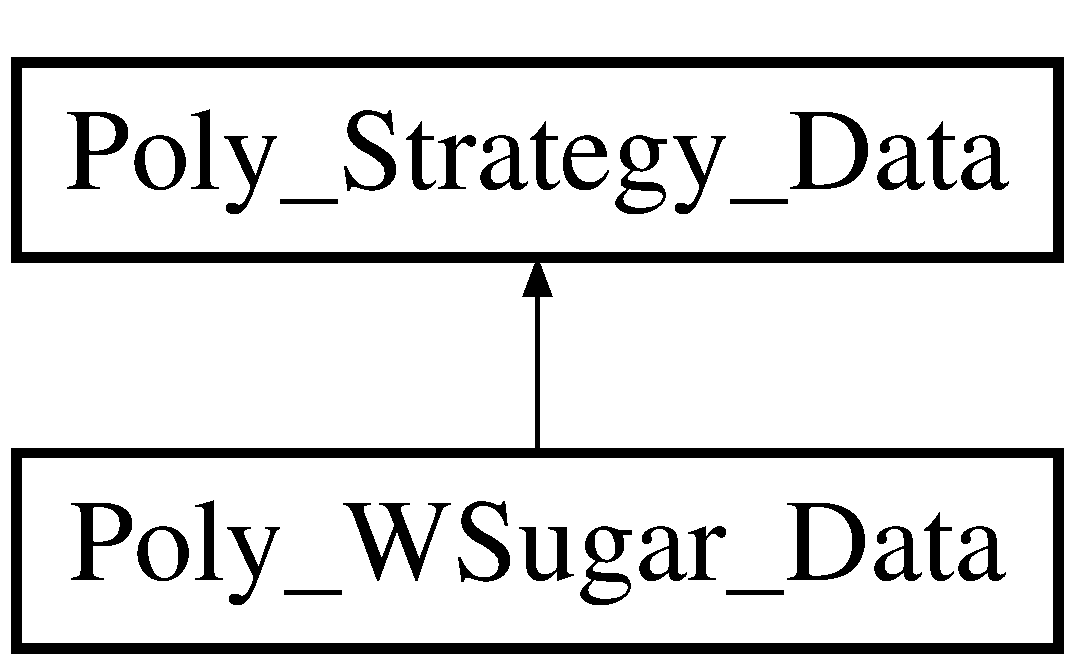
\includegraphics[height=2.000000cm]{group__strategygroup}
\end{center}
\end{figure}
\subsubsection*{Public Member Functions}
\begin{DoxyCompactItemize}
\item 
\hyperlink{group__strategygroup_a0d9e2f66a44f2e10d26b977c55650f7f}{Poly\+\_\+\+Sugar\+\_\+\+Data} (const \hyperlink{group__polygroup_class_abstract___polynomial}{Abstract\+\_\+\+Polynomial} $\ast$poly)
\begin{DoxyCompactList}\small\item\em records {\ttfamily poly} as the reference for {\ttfamily this} \end{DoxyCompactList}\item 
\mbox{\Hypertarget{group__strategygroup_ada533e5c56d7f53207a5e8093414dfb3}\label{group__strategygroup_ada533e5c56d7f53207a5e8093414dfb3}} 
virtual void \hyperlink{group__strategygroup_ada533e5c56d7f53207a5e8093414dfb3}{at\+\_\+generation\+\_\+tasks} ()
\begin{DoxyCompactList}\small\item\em sets the sugar to the largest total degree of a monomial in the assigned previously polynomial \end{DoxyCompactList}\item 
virtual void \hyperlink{group__strategygroup_aa80c660f10b1c5d0dd2a305d598685f5}{at\+\_\+generation\+\_\+tasks} (const \hyperlink{group__polygroup_class_monomial}{Monomial} \&t)
\begin{DoxyCompactList}\small\item\em sets the sugar to the largest total degree of a monomial in the product of the monomial and the previously assigned polynomial \end{DoxyCompactList}\item 
virtual bool \hyperlink{group__strategygroup_a73df53a8da9e4cfaf66202a1451d5b2e}{equivalent} (const \hyperlink{group__strategygroup_class_poly___strategy___data}{Poly\+\_\+\+Strategy\+\_\+\+Data} \&sd) const
\begin{DoxyCompactList}\small\item\em returns {\ttfamily true} iff the sugars are equal \end{DoxyCompactList}\item 
virtual bool \hyperlink{group__strategygroup_a9ccb90a43591e465479258bdf10b5b20}{first\+\_\+larger} (const \hyperlink{group__strategygroup_class_poly___strategy___data}{Poly\+\_\+\+Strategy\+\_\+\+Data} \&sd) const
\begin{DoxyCompactList}\small\item\em returns {\ttfamily true} iff {\ttfamily this} sugar is larger than {\ttfamily sd} 's \end{DoxyCompactList}\item 
virtual void \hyperlink{group__strategygroup_a1b2e8a7fe4fcd57555fa58e48620b2bf}{pre\+\_\+reduction\+\_\+tasks} (const E\+X\+P\+\_\+\+T\+Y\+PE $\ast$u, const \hyperlink{group__polygroup_class_abstract___polynomial}{Abstract\+\_\+\+Polynomial} \&g)
\begin{DoxyCompactList}\small\item\em re-\/evaluates the sugar, if need be \end{DoxyCompactList}\end{DoxyCompactItemize}
\begin{Indent}\textbf{ Basic properties}\par
\begin{DoxyCompactItemize}
\item 
\mbox{\Hypertarget{group__strategygroup_a3b6ef678b640a3138e43882b9d2dca5f}\label{group__strategygroup_a3b6ef678b640a3138e43882b9d2dca5f}} 
D\+E\+G\+\_\+\+T\+Y\+PE \hyperlink{group__strategygroup_a3b6ef678b640a3138e43882b9d2dca5f}{poly\+\_\+sugar} () const
\begin{DoxyCompactList}\small\item\em the sugar itself \end{DoxyCompactList}\item 
\mbox{\Hypertarget{group__strategygroup_a36704dfc77b9007bf5f249e55bfde0ef}\label{group__strategygroup_a36704dfc77b9007bf5f249e55bfde0ef}} 
virtual \hyperlink{group__strategygroup_ga0ee6c8e033547330e6b89929730007f4}{Strategy\+Flags} \hyperlink{group__strategygroup_a36704dfc77b9007bf5f249e55bfde0ef}{type} ()
\begin{DoxyCompactList}\small\item\em the strategy type \end{DoxyCompactList}\end{DoxyCompactItemize}
\end{Indent}
\begin{Indent}\textbf{ Modification}\par
\begin{DoxyCompactItemize}
\item 
\mbox{\Hypertarget{group__strategygroup_a945416871509370e2222c8c7abe01759}\label{group__strategygroup_a945416871509370e2222c8c7abe01759}} 
void \hyperlink{group__strategygroup_a945416871509370e2222c8c7abe01759}{force\+\_\+sugar} (D\+E\+G\+\_\+\+T\+Y\+PE new\+\_\+sugar)
\begin{DoxyCompactList}\small\item\em for those times when a different sugar is appropriate \end{DoxyCompactList}\end{DoxyCompactItemize}
\end{Indent}
\subsubsection*{Protected Attributes}
\begin{DoxyCompactItemize}
\item 
\mbox{\Hypertarget{group__strategygroup_a125902ea0a800d9545937930e4537040}\label{group__strategygroup_a125902ea0a800d9545937930e4537040}} 
unsigned long long \hyperlink{group__strategygroup_a125902ea0a800d9545937930e4537040}{sugar}
\begin{DoxyCompactList}\small\item\em the polynomial's sugar \end{DoxyCompactList}\end{DoxyCompactItemize}
\subsubsection*{Friends}
\begin{Indent}\textbf{ I/O}\par
\begin{DoxyCompactItemize}
\item 
\mbox{\Hypertarget{group__strategygroup_ade466c9119513ef40b2b6220a98a72e6}\label{group__strategygroup_ade466c9119513ef40b2b6220a98a72e6}} 
ostream \& {\bfseries operator$<$$<$} (ostream \&, const \hyperlink{group__strategygroup_class_poly___sugar___data}{Poly\+\_\+\+Sugar\+\_\+\+Data} \&)
\end{DoxyCompactItemize}
\end{Indent}


\paragraph{Constructor \& Destructor Documentation}
\mbox{\Hypertarget{group__strategygroup_a0d9e2f66a44f2e10d26b977c55650f7f}\label{group__strategygroup_a0d9e2f66a44f2e10d26b977c55650f7f}} 
\index{Poly\+\_\+\+Sugar\+\_\+\+Data@{Poly\+\_\+\+Sugar\+\_\+\+Data}!Poly\+\_\+\+Sugar\+\_\+\+Data@{Poly\+\_\+\+Sugar\+\_\+\+Data}}
\index{Poly\+\_\+\+Sugar\+\_\+\+Data@{Poly\+\_\+\+Sugar\+\_\+\+Data}!Poly\+\_\+\+Sugar\+\_\+\+Data@{Poly\+\_\+\+Sugar\+\_\+\+Data}}
\subparagraph{\texorpdfstring{Poly\+\_\+\+Sugar\+\_\+\+Data()}{Poly\_Sugar\_Data()}}
{\footnotesize\ttfamily Poly\+\_\+\+Sugar\+\_\+\+Data\+::\+Poly\+\_\+\+Sugar\+\_\+\+Data (\begin{DoxyParamCaption}\item[{const \hyperlink{group__polygroup_class_abstract___polynomial}{Abstract\+\_\+\+Polynomial} $\ast$}]{poly }\end{DoxyParamCaption})}



records {\ttfamily poly} as the reference for {\ttfamily this} 


\begin{DoxyParams}{Parameters}
{\em poly} & the polynomial whose sugar data {\ttfamily this} should be \\
\hline
\end{DoxyParams}


Definition at line 26 of file sugar\+\_\+strategy.\+cpp.



\paragraph{Member Function Documentation}
\mbox{\Hypertarget{group__strategygroup_aa80c660f10b1c5d0dd2a305d598685f5}\label{group__strategygroup_aa80c660f10b1c5d0dd2a305d598685f5}} 
\index{Poly\+\_\+\+Sugar\+\_\+\+Data@{Poly\+\_\+\+Sugar\+\_\+\+Data}!at\+\_\+generation\+\_\+tasks@{at\+\_\+generation\+\_\+tasks}}
\index{at\+\_\+generation\+\_\+tasks@{at\+\_\+generation\+\_\+tasks}!Poly\+\_\+\+Sugar\+\_\+\+Data@{Poly\+\_\+\+Sugar\+\_\+\+Data}}
\subparagraph{\texorpdfstring{at\+\_\+generation\+\_\+tasks()}{at\_generation\_tasks()}}
{\footnotesize\ttfamily void Poly\+\_\+\+Sugar\+\_\+\+Data\+::at\+\_\+generation\+\_\+tasks (\begin{DoxyParamCaption}\item[{const \hyperlink{group__polygroup_class_monomial}{Monomial} \&}]{t }\end{DoxyParamCaption})\hspace{0.3cm}{\ttfamily [virtual]}}



sets the sugar to the largest total degree of a monomial in the product of the monomial and the previously assigned polynomial 


\begin{DoxyParams}{Parameters}
{\em t} & a \hyperlink{group__polygroup_class_monomial}{Monomial} to multiply to {\ttfamily this} \\
\hline
\end{DoxyParams}


Reimplemented from \hyperlink{group__strategygroup_a6683749a5fb30b6f91075a28899fbfe7}{Poly\+\_\+\+Strategy\+\_\+\+Data}.



Definition at line 51 of file sugar\+\_\+strategy.\+cpp.

\mbox{\Hypertarget{group__strategygroup_a73df53a8da9e4cfaf66202a1451d5b2e}\label{group__strategygroup_a73df53a8da9e4cfaf66202a1451d5b2e}} 
\index{Poly\+\_\+\+Sugar\+\_\+\+Data@{Poly\+\_\+\+Sugar\+\_\+\+Data}!equivalent@{equivalent}}
\index{equivalent@{equivalent}!Poly\+\_\+\+Sugar\+\_\+\+Data@{Poly\+\_\+\+Sugar\+\_\+\+Data}}
\subparagraph{\texorpdfstring{equivalent()}{equivalent()}}
{\footnotesize\ttfamily bool Poly\+\_\+\+Sugar\+\_\+\+Data\+::equivalent (\begin{DoxyParamCaption}\item[{const \hyperlink{group__strategygroup_class_poly___strategy___data}{Poly\+\_\+\+Strategy\+\_\+\+Data} \&}]{sd }\end{DoxyParamCaption}) const\hspace{0.3cm}{\ttfamily [virtual]}}



returns {\ttfamily true} iff the sugars are equal 


\begin{DoxyParams}{Parameters}
{\em sd} & strategy data containing sugar \\
\hline
\end{DoxyParams}
\begin{DoxyReturn}{Returns}
{\ttfamily true} if and only if the sugar of {\ttfamily this} is equivalent to the sugar of {\ttfamily sd} 
\end{DoxyReturn}


Implements \hyperlink{group__strategygroup_aa82a57a8bf9b3c14fd65a573fd78a4a5}{Poly\+\_\+\+Strategy\+\_\+\+Data}.



Definition at line 31 of file sugar\+\_\+strategy.\+cpp.

\mbox{\Hypertarget{group__strategygroup_a9ccb90a43591e465479258bdf10b5b20}\label{group__strategygroup_a9ccb90a43591e465479258bdf10b5b20}} 
\index{Poly\+\_\+\+Sugar\+\_\+\+Data@{Poly\+\_\+\+Sugar\+\_\+\+Data}!first\+\_\+larger@{first\+\_\+larger}}
\index{first\+\_\+larger@{first\+\_\+larger}!Poly\+\_\+\+Sugar\+\_\+\+Data@{Poly\+\_\+\+Sugar\+\_\+\+Data}}
\subparagraph{\texorpdfstring{first\+\_\+larger()}{first\_larger()}}
{\footnotesize\ttfamily bool Poly\+\_\+\+Sugar\+\_\+\+Data\+::first\+\_\+larger (\begin{DoxyParamCaption}\item[{const \hyperlink{group__strategygroup_class_poly___strategy___data}{Poly\+\_\+\+Strategy\+\_\+\+Data} \&}]{sd }\end{DoxyParamCaption}) const\hspace{0.3cm}{\ttfamily [virtual]}}



returns {\ttfamily true} iff {\ttfamily this} sugar is larger than {\ttfamily sd} 's 


\begin{DoxyParams}{Parameters}
{\em sd} & strategy data containing sugar \\
\hline
\end{DoxyParams}
\begin{DoxyReturn}{Returns}
{\ttfamily true} if and only if {\ttfamily this} sugar is larger than {\ttfamily sd} 's 
\end{DoxyReturn}


Implements \hyperlink{group__strategygroup_a6cd4608015a6b0f06141b9b73b0d4137}{Poly\+\_\+\+Strategy\+\_\+\+Data}.



Definition at line 36 of file sugar\+\_\+strategy.\+cpp.

\mbox{\Hypertarget{group__strategygroup_a1b2e8a7fe4fcd57555fa58e48620b2bf}\label{group__strategygroup_a1b2e8a7fe4fcd57555fa58e48620b2bf}} 
\index{Poly\+\_\+\+Sugar\+\_\+\+Data@{Poly\+\_\+\+Sugar\+\_\+\+Data}!pre\+\_\+reduction\+\_\+tasks@{pre\+\_\+reduction\+\_\+tasks}}
\index{pre\+\_\+reduction\+\_\+tasks@{pre\+\_\+reduction\+\_\+tasks}!Poly\+\_\+\+Sugar\+\_\+\+Data@{Poly\+\_\+\+Sugar\+\_\+\+Data}}
\subparagraph{\texorpdfstring{pre\+\_\+reduction\+\_\+tasks()}{pre\_reduction\_tasks()}}
{\footnotesize\ttfamily void Poly\+\_\+\+Sugar\+\_\+\+Data\+::pre\+\_\+reduction\+\_\+tasks (\begin{DoxyParamCaption}\item[{const E\+X\+P\+\_\+\+T\+Y\+PE $\ast$}]{u,  }\item[{const \hyperlink{group__polygroup_class_abstract___polynomial}{Abstract\+\_\+\+Polynomial} \&}]{g }\end{DoxyParamCaption})\hspace{0.3cm}{\ttfamily [virtual]}}



re-\/evaluates the sugar, if need be 


\begin{DoxyParams}{Parameters}
{\em u} & exponent vector of a \hyperlink{group__polygroup_class_monomial}{Monomial} to multiply to {\ttfamily g}, then subtract from {\ttfamily this} \\
\hline
{\em g} & a polynomial \\
\hline
\end{DoxyParams}


Reimplemented from \hyperlink{group__strategygroup_a0d71db50c58a24f48f94eae6a48c2149}{Poly\+\_\+\+Strategy\+\_\+\+Data}.



Definition at line 61 of file sugar\+\_\+strategy.\+cpp.

\index{Poly\+\_\+\+W\+Sugar\+\_\+\+Data@{Poly\+\_\+\+W\+Sugar\+\_\+\+Data}}\label{class_poly___w_sugar___data}
\Hypertarget{group__strategygroup_class_poly___w_sugar___data}
\subsubsection{class Poly\+\_\+\+W\+Sugar\+\_\+\+Data}
polynomial-\/related data for a weighted sugar strategy 

\begin{DoxyAuthor}{Author}
John Perry 
\end{DoxyAuthor}
\begin{DoxyDate}{Date}
2016
\end{DoxyDate}
This strategy is based on a weight vector, rather than simply adding exponents. While the weight vector {\itshape can} be that of a weighted ordering, one is also free to use a different weight altogether. Simply supply the relevant data. 

Definition at line 39 of file weighted\+\_\+sugar\+\_\+strategy.\+hpp.

Inheritance diagram for Poly\+\_\+\+W\+Sugar\+\_\+\+Data\+:\begin{figure}[H]
\begin{center}
\leavevmode
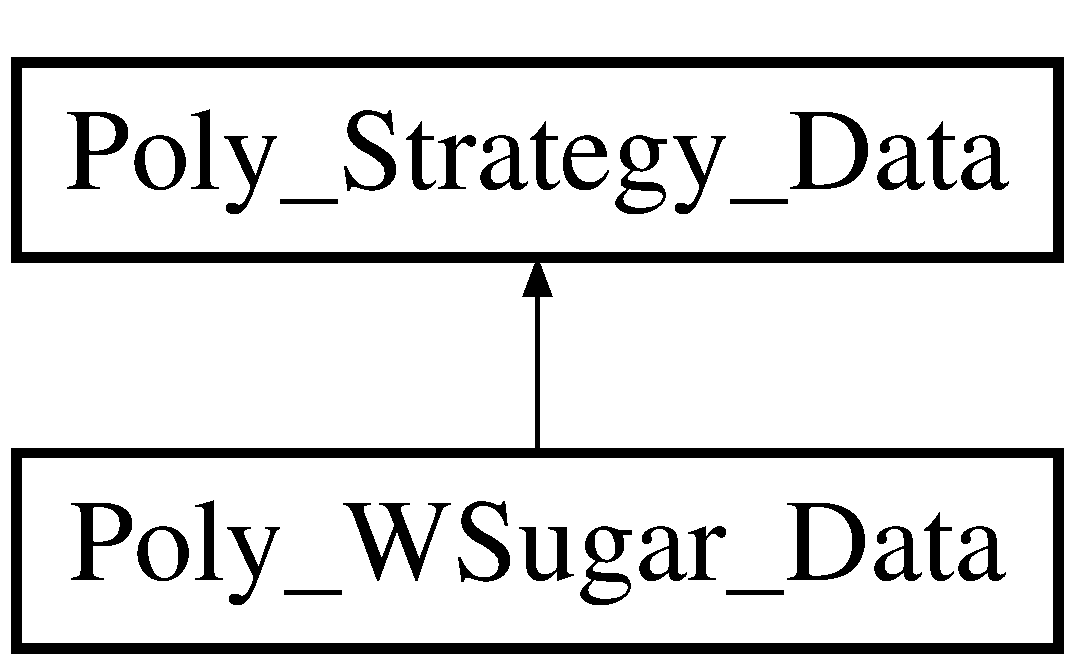
\includegraphics[height=2.000000cm]{group__strategygroup}
\end{center}
\end{figure}
\subsubsection*{Public Member Functions}
\begin{DoxyCompactItemize}
\item 
\hyperlink{group__strategygroup_a1f64d0099befd970d362c0166be1b652}{Poly\+\_\+\+W\+Sugar\+\_\+\+Data} (const \hyperlink{group__polygroup_class_abstract___polynomial}{Abstract\+\_\+\+Polynomial} $\ast$poly, const W\+T\+\_\+\+T\+Y\+PE $\ast$w)
\begin{DoxyCompactList}\small\item\em records {\ttfamily poly} as the reference for {\ttfamily this} \end{DoxyCompactList}\item 
\mbox{\Hypertarget{group__strategygroup_ac07ee9ee15bd97e5e8befb3f6cec3929}\label{group__strategygroup_ac07ee9ee15bd97e5e8befb3f6cec3929}} 
virtual void \hyperlink{group__strategygroup_ac07ee9ee15bd97e5e8befb3f6cec3929}{at\+\_\+generation\+\_\+tasks} ()
\begin{DoxyCompactList}\small\item\em sets the sugar to the largest weighted degree of a monomial in the assigned previously polynomial \end{DoxyCompactList}\item 
virtual void \hyperlink{group__strategygroup_ac58bd8d30e7e10dbbe8e86b1d9d04376}{at\+\_\+generation\+\_\+tasks} (const \hyperlink{group__polygroup_class_monomial}{Monomial} \&t)
\begin{DoxyCompactList}\small\item\em sets the sugar to the largest weighted degree of a monomial in the product of the monomial and the previously assigned polynomial \end{DoxyCompactList}\item 
virtual bool \hyperlink{group__strategygroup_a50b4b29d57fb8bed56174733207369dd}{equivalent} (const \hyperlink{group__strategygroup_class_poly___strategy___data}{Poly\+\_\+\+Strategy\+\_\+\+Data} \&sd) const
\begin{DoxyCompactList}\small\item\em returns {\ttfamily true} iff the sugars are equal \end{DoxyCompactList}\item 
virtual bool \hyperlink{group__strategygroup_a83a899b8195beed8d72d692fe4c228a3}{first\+\_\+larger} (const \hyperlink{group__strategygroup_class_poly___strategy___data}{Poly\+\_\+\+Strategy\+\_\+\+Data} \&sd) const
\begin{DoxyCompactList}\small\item\em returns {\ttfamily true} iff {\ttfamily this} sugar is larger than {\ttfamily sd} 's \end{DoxyCompactList}\item 
virtual void \hyperlink{group__strategygroup_a4a34039eb50a2294d2aaf6245c1833b8}{pre\+\_\+reduction\+\_\+tasks} (const E\+X\+P\+\_\+\+T\+Y\+PE $\ast$u, const \hyperlink{group__polygroup_class_abstract___polynomial}{Abstract\+\_\+\+Polynomial} \&g)
\begin{DoxyCompactList}\small\item\em re-\/evaluates the sugar, if need be \end{DoxyCompactList}\end{DoxyCompactItemize}
\begin{Indent}\textbf{ Basic properties}\par
\begin{DoxyCompactItemize}
\item 
\mbox{\Hypertarget{group__strategygroup_a472c39541209b6738cb497ebc3c9e205}\label{group__strategygroup_a472c39541209b6738cb497ebc3c9e205}} 
\hyperlink{group__strategygroup_ga0ee6c8e033547330e6b89929730007f4}{Strategy\+Flags} \hyperlink{group__strategygroup_a472c39541209b6738cb497ebc3c9e205}{type} ()
\begin{DoxyCompactList}\small\item\em type of strategy \end{DoxyCompactList}\item 
\mbox{\Hypertarget{group__strategygroup_a2d369a1ab46cf990413f190f22203a3d}\label{group__strategygroup_a2d369a1ab46cf990413f190f22203a3d}} 
D\+E\+G\+\_\+\+T\+Y\+PE \hyperlink{group__strategygroup_a2d369a1ab46cf990413f190f22203a3d}{poly\+\_\+sugar} () const
\begin{DoxyCompactList}\small\item\em the sugar itself \end{DoxyCompactList}\item 
\mbox{\Hypertarget{group__strategygroup_a0ac423ed3a00a9b7e71dc8103116c82c}\label{group__strategygroup_a0ac423ed3a00a9b7e71dc8103116c82c}} 
const W\+T\+\_\+\+T\+Y\+PE $\ast$ \hyperlink{group__strategygroup_a0ac423ed3a00a9b7e71dc8103116c82c}{weighting} () const
\begin{DoxyCompactList}\small\item\em the weights used to compute the sugar \end{DoxyCompactList}\end{DoxyCompactItemize}
\end{Indent}
\begin{Indent}\textbf{ Modification}\par
\begin{DoxyCompactItemize}
\item 
\mbox{\Hypertarget{group__strategygroup_aa8fbd9cf3d9e391a9db0ececdabea03f}\label{group__strategygroup_aa8fbd9cf3d9e391a9db0ececdabea03f}} 
void \hyperlink{group__strategygroup_aa8fbd9cf3d9e391a9db0ececdabea03f}{change\+\_\+weights} (const W\+T\+\_\+\+T\+Y\+PE $\ast$w)
\begin{DoxyCompactList}\small\item\em changes the weights used to compute the sugar to {\ttfamily w} \end{DoxyCompactList}\end{DoxyCompactItemize}
\end{Indent}
\subsubsection*{Protected Attributes}
\begin{DoxyCompactItemize}
\item 
\mbox{\Hypertarget{group__strategygroup_a8a3f679ee5536587a4794a8c20b92cb9}\label{group__strategygroup_a8a3f679ee5536587a4794a8c20b92cb9}} 
D\+E\+G\+\_\+\+T\+Y\+PE \hyperlink{group__strategygroup_a8a3f679ee5536587a4794a8c20b92cb9}{sugar}
\begin{DoxyCompactList}\small\item\em the polynomial's sugar \end{DoxyCompactList}\item 
\mbox{\Hypertarget{group__strategygroup_acbe98e7f937ab0c074a732becdd8c619}\label{group__strategygroup_acbe98e7f937ab0c074a732becdd8c619}} 
const W\+T\+\_\+\+T\+Y\+PE $\ast$ \hyperlink{group__strategygroup_acbe98e7f937ab0c074a732becdd8c619}{weights}
\begin{DoxyCompactList}\small\item\em pointer to the weights \end{DoxyCompactList}\end{DoxyCompactItemize}
\subsubsection*{Friends}
\begin{Indent}\textbf{ I/O}\par
\begin{DoxyCompactItemize}
\item 
\mbox{\Hypertarget{group__strategygroup_aaa672dbee5334fe3b57404502489f800}\label{group__strategygroup_aaa672dbee5334fe3b57404502489f800}} 
ostream \& {\bfseries operator$<$$<$} (ostream \&, const \hyperlink{group__strategygroup_class_poly___w_sugar___data}{Poly\+\_\+\+W\+Sugar\+\_\+\+Data} \&)
\end{DoxyCompactItemize}
\end{Indent}


\paragraph{Constructor \& Destructor Documentation}
\mbox{\Hypertarget{group__strategygroup_a1f64d0099befd970d362c0166be1b652}\label{group__strategygroup_a1f64d0099befd970d362c0166be1b652}} 
\index{Poly\+\_\+\+W\+Sugar\+\_\+\+Data@{Poly\+\_\+\+W\+Sugar\+\_\+\+Data}!Poly\+\_\+\+W\+Sugar\+\_\+\+Data@{Poly\+\_\+\+W\+Sugar\+\_\+\+Data}}
\index{Poly\+\_\+\+W\+Sugar\+\_\+\+Data@{Poly\+\_\+\+W\+Sugar\+\_\+\+Data}!Poly\+\_\+\+W\+Sugar\+\_\+\+Data@{Poly\+\_\+\+W\+Sugar\+\_\+\+Data}}
\subparagraph{\texorpdfstring{Poly\+\_\+\+W\+Sugar\+\_\+\+Data()}{Poly\_WSugar\_Data()}}
{\footnotesize\ttfamily Poly\+\_\+\+W\+Sugar\+\_\+\+Data\+::\+Poly\+\_\+\+W\+Sugar\+\_\+\+Data (\begin{DoxyParamCaption}\item[{const \hyperlink{group__polygroup_class_abstract___polynomial}{Abstract\+\_\+\+Polynomial} $\ast$}]{poly,  }\item[{const W\+T\+\_\+\+T\+Y\+PE $\ast$}]{w }\end{DoxyParamCaption})}



records {\ttfamily poly} as the reference for {\ttfamily this} 

This expects the weights to be as long as the number of monomials. It copies the list, so you can subsequently modify it without subsequently affecting correctness. \begin{DoxyWarning}{Warning}
The weights are not copied. Please do not modify them, as behavior is hard to predict in this case. It is predictable, but it's likely highly undesirable. Better to create a new \hyperlink{group__strategygroup_class_poly___w_sugar___data}{Poly\+\_\+\+W\+Sugar\+\_\+\+Data} instead. 
\end{DoxyWarning}

\begin{DoxyParams}{Parameters}
{\em poly} & polynomial whose sugar {\ttfamily this} is \\
\hline
{\em w} & weight vector to compute weighted sugar \\
\hline
\end{DoxyParams}


Definition at line 27 of file weighted\+\_\+sugar\+\_\+strategy.\+cpp.



\paragraph{Member Function Documentation}
\mbox{\Hypertarget{group__strategygroup_ac58bd8d30e7e10dbbe8e86b1d9d04376}\label{group__strategygroup_ac58bd8d30e7e10dbbe8e86b1d9d04376}} 
\index{Poly\+\_\+\+W\+Sugar\+\_\+\+Data@{Poly\+\_\+\+W\+Sugar\+\_\+\+Data}!at\+\_\+generation\+\_\+tasks@{at\+\_\+generation\+\_\+tasks}}
\index{at\+\_\+generation\+\_\+tasks@{at\+\_\+generation\+\_\+tasks}!Poly\+\_\+\+W\+Sugar\+\_\+\+Data@{Poly\+\_\+\+W\+Sugar\+\_\+\+Data}}
\subparagraph{\texorpdfstring{at\+\_\+generation\+\_\+tasks()}{at\_generation\_tasks()}}
{\footnotesize\ttfamily void Poly\+\_\+\+W\+Sugar\+\_\+\+Data\+::at\+\_\+generation\+\_\+tasks (\begin{DoxyParamCaption}\item[{const \hyperlink{group__polygroup_class_monomial}{Monomial} \&}]{t }\end{DoxyParamCaption})\hspace{0.3cm}{\ttfamily [virtual]}}



sets the sugar to the largest weighted degree of a monomial in the product of the monomial and the previously assigned polynomial 


\begin{DoxyParams}{Parameters}
{\em t} & a \hyperlink{group__polygroup_class_monomial}{Monomial} to multiply to {\ttfamily this} \\
\hline
\end{DoxyParams}


Reimplemented from \hyperlink{group__strategygroup_a6683749a5fb30b6f91075a28899fbfe7}{Poly\+\_\+\+Strategy\+\_\+\+Data}.



Definition at line 56 of file weighted\+\_\+sugar\+\_\+strategy.\+cpp.

\mbox{\Hypertarget{group__strategygroup_a50b4b29d57fb8bed56174733207369dd}\label{group__strategygroup_a50b4b29d57fb8bed56174733207369dd}} 
\index{Poly\+\_\+\+W\+Sugar\+\_\+\+Data@{Poly\+\_\+\+W\+Sugar\+\_\+\+Data}!equivalent@{equivalent}}
\index{equivalent@{equivalent}!Poly\+\_\+\+W\+Sugar\+\_\+\+Data@{Poly\+\_\+\+W\+Sugar\+\_\+\+Data}}
\subparagraph{\texorpdfstring{equivalent()}{equivalent()}}
{\footnotesize\ttfamily bool Poly\+\_\+\+W\+Sugar\+\_\+\+Data\+::equivalent (\begin{DoxyParamCaption}\item[{const \hyperlink{group__strategygroup_class_poly___strategy___data}{Poly\+\_\+\+Strategy\+\_\+\+Data} \&}]{sd }\end{DoxyParamCaption}) const\hspace{0.3cm}{\ttfamily [virtual]}}



returns {\ttfamily true} iff the sugars are equal 


\begin{DoxyParams}{Parameters}
{\em sd} & sugar data to compare with {\ttfamily this} \\
\hline
\end{DoxyParams}
\begin{DoxyReturn}{Returns}
true if and only if {\ttfamily this} has sugar comparable to {\ttfamily sd} 
\end{DoxyReturn}


Implements \hyperlink{group__strategygroup_aa82a57a8bf9b3c14fd65a573fd78a4a5}{Poly\+\_\+\+Strategy\+\_\+\+Data}.



Definition at line 35 of file weighted\+\_\+sugar\+\_\+strategy.\+cpp.

\mbox{\Hypertarget{group__strategygroup_a83a899b8195beed8d72d692fe4c228a3}\label{group__strategygroup_a83a899b8195beed8d72d692fe4c228a3}} 
\index{Poly\+\_\+\+W\+Sugar\+\_\+\+Data@{Poly\+\_\+\+W\+Sugar\+\_\+\+Data}!first\+\_\+larger@{first\+\_\+larger}}
\index{first\+\_\+larger@{first\+\_\+larger}!Poly\+\_\+\+W\+Sugar\+\_\+\+Data@{Poly\+\_\+\+W\+Sugar\+\_\+\+Data}}
\subparagraph{\texorpdfstring{first\+\_\+larger()}{first\_larger()}}
{\footnotesize\ttfamily bool Poly\+\_\+\+W\+Sugar\+\_\+\+Data\+::first\+\_\+larger (\begin{DoxyParamCaption}\item[{const \hyperlink{group__strategygroup_class_poly___strategy___data}{Poly\+\_\+\+Strategy\+\_\+\+Data} \&}]{sd }\end{DoxyParamCaption}) const\hspace{0.3cm}{\ttfamily [virtual]}}



returns {\ttfamily true} iff {\ttfamily this} sugar is larger than {\ttfamily sd} 's 


\begin{DoxyParams}{Parameters}
{\em sd} & sugar data to compare with {\ttfamily this} \\
\hline
\end{DoxyParams}
\begin{DoxyReturn}{Returns}
{\ttfamily true} if and only if {\ttfamily this} has larger sugar than {\ttfamily sd} 
\end{DoxyReturn}


Implements \hyperlink{group__strategygroup_a6cd4608015a6b0f06141b9b73b0d4137}{Poly\+\_\+\+Strategy\+\_\+\+Data}.



Definition at line 40 of file weighted\+\_\+sugar\+\_\+strategy.\+cpp.

\mbox{\Hypertarget{group__strategygroup_a4a34039eb50a2294d2aaf6245c1833b8}\label{group__strategygroup_a4a34039eb50a2294d2aaf6245c1833b8}} 
\index{Poly\+\_\+\+W\+Sugar\+\_\+\+Data@{Poly\+\_\+\+W\+Sugar\+\_\+\+Data}!pre\+\_\+reduction\+\_\+tasks@{pre\+\_\+reduction\+\_\+tasks}}
\index{pre\+\_\+reduction\+\_\+tasks@{pre\+\_\+reduction\+\_\+tasks}!Poly\+\_\+\+W\+Sugar\+\_\+\+Data@{Poly\+\_\+\+W\+Sugar\+\_\+\+Data}}
\subparagraph{\texorpdfstring{pre\+\_\+reduction\+\_\+tasks()}{pre\_reduction\_tasks()}}
{\footnotesize\ttfamily void Poly\+\_\+\+W\+Sugar\+\_\+\+Data\+::pre\+\_\+reduction\+\_\+tasks (\begin{DoxyParamCaption}\item[{const E\+X\+P\+\_\+\+T\+Y\+PE $\ast$}]{u,  }\item[{const \hyperlink{group__polygroup_class_abstract___polynomial}{Abstract\+\_\+\+Polynomial} \&}]{g }\end{DoxyParamCaption})\hspace{0.3cm}{\ttfamily [virtual]}}



re-\/evaluates the sugar, if need be 


\begin{DoxyParams}{Parameters}
{\em u} & monomial to multiply to {\ttfamily g}, then reduce {\ttfamily this} by the product \\
\hline
{\em g} & a polynomial whose leading monomial divides {\ttfamily this} \\
\hline
\end{DoxyParams}


Reimplemented from \hyperlink{group__strategygroup_a0d71db50c58a24f48f94eae6a48c2149}{Poly\+\_\+\+Strategy\+\_\+\+Data}.



Definition at line 71 of file weighted\+\_\+sugar\+\_\+strategy.\+cpp.



\subsection{Enumeration Type Documentation}
\mbox{\Hypertarget{group__strategygroup_ga0ee6c8e033547330e6b89929730007f4}\label{group__strategygroup_ga0ee6c8e033547330e6b89929730007f4}} 
\index{Strategies@{Strategies}!Strategy\+Flags@{Strategy\+Flags}}
\index{Strategy\+Flags@{Strategy\+Flags}!Strategies@{Strategies}}
\subsubsection{\texorpdfstring{Strategy\+Flags}{StrategyFlags}}
{\footnotesize\ttfamily enum \hyperlink{group__strategygroup_ga0ee6c8e033547330e6b89929730007f4}{Strategy\+Flags}\hspace{0.3cm}{\ttfamily [strong]}}



flag indicating which strategy to use for computation 

\begin{DoxyAuthor}{Author}
John Perry 
\end{DoxyAuthor}
\begin{DoxyDate}{Date}
2016 
\end{DoxyDate}


Definition at line 34 of file strategies.\+hpp.


\hypertarget{group__utils}{}\section{Utilities}
\label{group__utils}\index{Utilities@{Utilities}}


Useful functions and classes that don\textquotesingle{}t fit in easily elsewhere.  


\subsection*{Functions}
\begin{DoxyCompactItemize}
\item 
void \hyperlink{group__utils_gaefe33f79de88accbc6f455e91dab9288}{divide\+\_\+by\+\_\+common\+\_\+term} (C\+O\+E\+F\+\_\+\+T\+Y\+PE \&, U\+C\+O\+E\+F\+\_\+\+T\+Y\+PE \&)
\begin{DoxyCompactList}\small\item\em divides out the common term of the two given numbers \end{DoxyCompactList}\item 
void \hyperlink{group__utils_ga72d205e8226d578b892515edc527cc83}{user\+\_\+interface} ()
\begin{DoxyCompactList}\small\item\em reads ideal definition from {\ttfamily cin}, then reads options for computation, writes Gr\"{o}bner basis to {\ttfamily cout} \end{DoxyCompactList}\end{DoxyCompactItemize}


\subsection{Detailed Description}
Useful functions and classes that don\textquotesingle{}t fit in easily elsewhere. 



\subsection{Function Documentation}
\mbox{\Hypertarget{group__utils_gaefe33f79de88accbc6f455e91dab9288}\label{group__utils_gaefe33f79de88accbc6f455e91dab9288}} 
\index{Utilities@{Utilities}!divide\+\_\+by\+\_\+common\+\_\+term@{divide\+\_\+by\+\_\+common\+\_\+term}}
\index{divide\+\_\+by\+\_\+common\+\_\+term@{divide\+\_\+by\+\_\+common\+\_\+term}!Utilities@{Utilities}}
\subsubsection{\texorpdfstring{divide\+\_\+by\+\_\+common\+\_\+term()}{divide\_by\_common\_term()}}
{\footnotesize\ttfamily void divide\+\_\+by\+\_\+common\+\_\+term (\begin{DoxyParamCaption}\item[{C\+O\+E\+F\+\_\+\+T\+Y\+PE \&}]{,  }\item[{U\+C\+O\+E\+F\+\_\+\+T\+Y\+PE \&}]{ }\end{DoxyParamCaption})}



divides out the common term of the two given numbers 

\begin{DoxyAuthor}{Author}
John Perry 
\end{DoxyAuthor}
\begin{DoxyDate}{Date}
2016
\end{DoxyDate}
Useful for simplifying terms of \hyperlink{group__polygroup_class_dense___univariate___rational___polynomial}{Dense\+\_\+\+Univariate\+\_\+\+Rational\+\_\+\+Polynomial}. Uses the (simple) Euclidean Algorithm to determine the gcd. \mbox{\Hypertarget{group__utils_ga72d205e8226d578b892515edc527cc83}\label{group__utils_ga72d205e8226d578b892515edc527cc83}} 
\index{Utilities@{Utilities}!user\+\_\+interface@{user\+\_\+interface}}
\index{user\+\_\+interface@{user\+\_\+interface}!Utilities@{Utilities}}
\subsubsection{\texorpdfstring{user\+\_\+interface()}{user\_interface()}}
{\footnotesize\ttfamily void user\+\_\+interface (\begin{DoxyParamCaption}{ }\end{DoxyParamCaption})}



reads ideal definition from {\ttfamily cin}, then reads options for computation, writes Gr\"{o}bner basis to {\ttfamily cout} 

\begin{DoxyAuthor}{Author}
John Perry 
\end{DoxyAuthor}
\begin{DoxyDate}{Date}
2017 
\end{DoxyDate}
\begin{DoxyReturn}{Returns}
0 if success, nonzero otherwise
\end{DoxyReturn}
The definition of the ideal should take place as follows, {\bfseries in this order}. Bad Things Will Happen\textsuperscript{TM} if you do not heed. The good news is that the program prompts the user.
\begin{DoxyEnumerate}
\item a prime number, which defines the base field
\item the number of indeterminates
\item whether to specify the indeterminates' names
\item if so, the indeterminates' names
\item the number of polynomials
\item the definition of the polynomials (each terminated by a new line)
\item static or dynamic computation
\item if dynamic,
\begin{DoxyEnumerate}
\item which solver (\hyperlink{group___c_l_s_solvers_class_l_p___solver}{L\+P\+\_\+\+Solver})
\item which heuristic (Dynamic\+Heuristic)
\item whether to perform a global analysis of the input The code has some other options, but they are mere curiosities for the time being. 
\end{DoxyEnumerate}
\end{DoxyEnumerate}\begin{Desc}
\item[Examples\+: ]\par
\hyperlink{user_interface_8cpp-example}{user\+\_\+interface.\+cpp}.\end{Desc}


Definition at line 58 of file user\+\_\+interface.\+cpp.


\chapter{Namespace Documentation}
\hypertarget{namespace_dynamic___engine}{}\section{Dynamic\+\_\+\+Engine Namespace Reference}
\label{namespace_dynamic___engine}\index{Dynamic\+\_\+\+Engine@{Dynamic\+\_\+\+Engine}}


Namespace for functions directly related to dynamic computation of a Gr\"{o}bner basis.  


\subsection*{Classes}
\begin{DoxyCompactItemize}
\item 
class \hyperlink{group___g_b_computation_class_dynamic___engine_1_1_p_p___with___ideal}{P\+P\+\_\+\+With\+\_\+\+Ideal}
\begin{DoxyCompactList}\small\item\em Used to associate a potential leading power product with the resulting monomial ideal if it were chosen as the actual leading power product.  \hyperlink{group___g_b_computation_class_dynamic___engine_1_1_p_p___with___ideal}{More...}\end{DoxyCompactList}\end{DoxyCompactItemize}
\subsection*{Enumerations}
\begin{DoxyCompactItemize}
\item 
enum \hyperlink{group___g_b_computation_ga819b1fd40d9a40ff303df3b90647ecb0}{Dynamic\+\_\+\+Heuristic} \{ \newline
{\bfseries M\+I\+N\+\_\+\+H\+E\+U\+R\+I\+S\+T\+IC} = 0, 
{\bfseries O\+R\+D\+\_\+\+H\+I\+L\+B\+E\+R\+T\+\_\+\+T\+H\+E\+N\+\_\+\+L\+EX}, 
{\bfseries O\+R\+D\+\_\+\+H\+I\+L\+B\+E\+R\+T\+\_\+\+T\+H\+E\+N\+\_\+\+D\+EG}, 
{\bfseries G\+R\+A\+D\+\_\+\+H\+I\+L\+B\+\_\+\+T\+H\+E\+N\+\_\+\+D\+EG}, 
\newline
{\bfseries M\+I\+N\+\_\+\+C\+R\+I\+T\+\_\+\+P\+A\+I\+RS}, 
{\bfseries G\+R\+A\+D\+\_\+\+M\+I\+N\+\_\+\+C\+R\+I\+T\+\_\+\+P\+A\+I\+RS}, 
{\bfseries B\+E\+T\+T\+I\+\_\+\+H\+I\+L\+B\+E\+R\+T\+\_\+\+D\+EG}, 
{\bfseries B\+I\+G\+\_\+\+B\+E\+T\+T\+I\+\_\+\+H\+I\+L\+B\+E\+R\+T\+\_\+\+D\+EG}, 
\newline
{\bfseries G\+R\+A\+D\+\_\+\+B\+E\+T\+T\+I\+\_\+\+H\+I\+L\+B\+E\+R\+T\+\_\+\+D\+EG}, 
{\bfseries S\+M\+O\+O\+T\+H\+E\+S\+T\+\_\+\+D\+E\+G\+R\+E\+ES}, 
{\bfseries L\+A\+R\+G\+E\+S\+T\+\_\+\+M\+A\+X\+\_\+\+C\+O\+M\+P\+O\+N\+E\+NT}, 
{\bfseries D\+E\+G\+\_\+\+T\+H\+E\+N\+\_\+\+G\+R\+A\+D\+\_\+\+H\+I\+LB}, 
\newline
{\bfseries D\+E\+G\+\_\+\+T\+H\+E\+N\+\_\+\+O\+R\+D\+\_\+\+H\+I\+L\+B\+E\+RT}, 
{\bfseries M\+A\+X\+\_\+\+H\+E\+U\+R\+I\+S\+T\+IC}
 \}\begin{DoxyCompactList}\small\item\em values for the heuristic, as in {\ttfamily \hyperlink{group___g_b_computation_gaa01d88c431b84deabf51ee116d7d2a0e}{select\+\_\+monomial()}} \end{DoxyCompactList}
\end{DoxyCompactItemize}
\subsection*{Functions}
\begin{DoxyCompactItemize}
\item 
void \hyperlink{group___g_b_computation_gabe68a8de3b87f6cc69e64fff39b71a81}{compatible\+\_\+pp} (\hyperlink{group__polygroup_class_monomial}{Monomial} current\+L\+PP, const set$<$ \hyperlink{group__polygroup_class_monomial}{Monomial} $>$ \&all\+P\+Ps, set$<$ \hyperlink{group__polygroup_class_monomial}{Monomial} $>$ \&result, set$<$ \hyperlink{group__polygroup_class_monomial}{Monomial} $>$ \&boundary\+\_\+mons, \hyperlink{group___c_l_s_solvers_class_l_p___solvers_1_1_l_p___solver}{L\+P\+\_\+\+Solver} $\ast$skel)
\begin{DoxyCompactList}\small\item\em Compute the compatible leading monomials of a polynomial. \end{DoxyCompactList}\item 
void \hyperlink{group___g_b_computation_gaf0ec0ad4f8430c46fc90c16104020f16}{constraints\+\_\+for\+\_\+new\+\_\+pp} (const \hyperlink{group___g_b_computation_class_dynamic___engine_1_1_p_p___with___ideal}{P\+P\+\_\+\+With\+\_\+\+Ideal} \&pp\+\_\+I, const set$<$ \hyperlink{group__polygroup_class_monomial}{Monomial} $>$ \&monomials\+For\+Comparison, vector$<$ \hyperlink{group___c_l_s_solvers_class_l_p___solvers_1_1_constraint}{Constraint} $>$ \&result)
\begin{DoxyCompactList}\small\item\em Create constraints for a candidate L\+PP. \end{DoxyCompactList}\item 
int \hyperlink{group___g_b_computation_ga9be1af3b4560bec7a8f17c5716e33ee7}{hilbert\+\_\+cmp} (const \hyperlink{group__polygroup_class_dense___univariate___integer___polynomial}{Dense\+\_\+\+Univariate\+\_\+\+Integer\+\_\+\+Polynomial} \&hn1, const \hyperlink{group__polygroup_class_dense___univariate___rational___polynomial}{Dense\+\_\+\+Univariate\+\_\+\+Rational\+\_\+\+Polynomial} \&hp1, const \hyperlink{group__polygroup_class_dense___univariate___integer___polynomial}{Dense\+\_\+\+Univariate\+\_\+\+Integer\+\_\+\+Polynomial} \&hn2, const \hyperlink{group__polygroup_class_dense___univariate___rational___polynomial}{Dense\+\_\+\+Univariate\+\_\+\+Rational\+\_\+\+Polynomial} \&hp2)
\begin{DoxyCompactList}\small\item\em compares two Hilbert functions, using polynomial and numerator \end{DoxyCompactList}\item 
bool \hyperlink{namespace_dynamic___engine_ae09287ccff877cf16afbde841c738b9b}{less\+\_\+by\+\_\+betti} (\hyperlink{group___g_b_computation_class_dynamic___engine_1_1_p_p___with___ideal}{P\+P\+\_\+\+With\+\_\+\+Ideal} \&a, \hyperlink{group___g_b_computation_class_dynamic___engine_1_1_p_p___with___ideal}{P\+P\+\_\+\+With\+\_\+\+Ideal} \&b)
\begin{DoxyCompactList}\small\item\em compares the desirability of two potential expansions of a monomial ideal via the standard graded Betti heuristic \end{DoxyCompactList}\item 
bool \hyperlink{namespace_dynamic___engine_a083c09fdc98db92614d126a5cca19a24}{less\+\_\+by\+\_\+big\+\_\+betti} (\hyperlink{group___g_b_computation_class_dynamic___engine_1_1_p_p___with___ideal}{P\+P\+\_\+\+With\+\_\+\+Ideal} \&a, \hyperlink{group___g_b_computation_class_dynamic___engine_1_1_p_p___with___ideal}{P\+P\+\_\+\+With\+\_\+\+Ideal} \&b)
\begin{DoxyCompactList}\small\item\em compares the desirability of two potential expansions of a monomial ideal via the ``Big Betti'' heuristic \end{DoxyCompactList}\item 
bool \hyperlink{namespace_dynamic___engine_ab5f217efe789e73d511ab04ae93942f1}{less\+\_\+by\+\_\+degree\+\_\+then\+\_\+grad\+\_\+hilbert} (\hyperlink{group___g_b_computation_class_dynamic___engine_1_1_p_p___with___ideal}{P\+P\+\_\+\+With\+\_\+\+Ideal} \&a, \hyperlink{group___g_b_computation_class_dynamic___engine_1_1_p_p___with___ideal}{P\+P\+\_\+\+With\+\_\+\+Ideal} \&b)
\begin{DoxyCompactList}\small\item\em compares the desirability of two potential expansions of a monomial ideal via the weighted degree+graded Hilbert heuristic \end{DoxyCompactList}\item 
bool \hyperlink{namespace_dynamic___engine_ae94f12023f4a0c1bf246afc31cd0538e}{less\+\_\+by\+\_\+degree\+\_\+then\+\_\+hilbert} (\hyperlink{group___g_b_computation_class_dynamic___engine_1_1_p_p___with___ideal}{P\+P\+\_\+\+With\+\_\+\+Ideal} \&a, \hyperlink{group___g_b_computation_class_dynamic___engine_1_1_p_p___with___ideal}{P\+P\+\_\+\+With\+\_\+\+Ideal} \&b)
\begin{DoxyCompactList}\small\item\em compares the desirability of two potential expansions of a monomial ideal via the degree+\+Hilbert heuristic \end{DoxyCompactList}\item 
bool \hyperlink{namespace_dynamic___engine_a8c67515d04de029583ba590b2ca4d6e4}{less\+\_\+by\+\_\+grad\+\_\+betti} (\hyperlink{group___g_b_computation_class_dynamic___engine_1_1_p_p___with___ideal}{P\+P\+\_\+\+With\+\_\+\+Ideal} \&a, \hyperlink{group___g_b_computation_class_dynamic___engine_1_1_p_p___with___ideal}{P\+P\+\_\+\+With\+\_\+\+Ideal} \&b)
\begin{DoxyCompactList}\small\item\em the graded Betti heuristic with a non-\/standard grading \end{DoxyCompactList}\item 
bool \hyperlink{namespace_dynamic___engine_a9a6525d0f50053349c5573422f025c22}{less\+\_\+by\+\_\+grad\+\_\+hilbert\+\_\+then\+\_\+degree} (\hyperlink{group___g_b_computation_class_dynamic___engine_1_1_p_p___with___ideal}{P\+P\+\_\+\+With\+\_\+\+Ideal} \&a, \hyperlink{group___g_b_computation_class_dynamic___engine_1_1_p_p___with___ideal}{P\+P\+\_\+\+With\+\_\+\+Ideal} \&b)
\begin{DoxyCompactList}\small\item\em compares the desirability of two potential expansions of a monomial ideal via the graded Hilbert+weighted degree heuristic \end{DoxyCompactList}\item 
bool \hyperlink{namespace_dynamic___engine_acb9d5de295d3d96abfa40dd47ae41c1f}{less\+\_\+by\+\_\+hilbert} (\hyperlink{group___g_b_computation_class_dynamic___engine_1_1_p_p___with___ideal}{P\+P\+\_\+\+With\+\_\+\+Ideal} \&a, \hyperlink{group___g_b_computation_class_dynamic___engine_1_1_p_p___with___ideal}{P\+P\+\_\+\+With\+\_\+\+Ideal} \&b)
\begin{DoxyCompactList}\small\item\em compares the desirability of two potential expansions of a monomial ideal via the Hilbert heuristic \end{DoxyCompactList}\item 
bool \hyperlink{namespace_dynamic___engine_afe48703afece2137e511824b00ccad39}{less\+\_\+by\+\_\+hilbert\+\_\+then\+\_\+degree} (\hyperlink{group___g_b_computation_class_dynamic___engine_1_1_p_p___with___ideal}{P\+P\+\_\+\+With\+\_\+\+Ideal} \&a, \hyperlink{group___g_b_computation_class_dynamic___engine_1_1_p_p___with___ideal}{P\+P\+\_\+\+With\+\_\+\+Ideal} \&b)
\begin{DoxyCompactList}\small\item\em compares the desirability of two potential expansions of a monomial ideal via the Hilbert+degree heuristic \end{DoxyCompactList}\item 
bool \hyperlink{namespace_dynamic___engine_acbc39a829236f4021485cc631f030264}{less\+\_\+by\+\_\+largest\+\_\+max\+\_\+component} (\hyperlink{group___g_b_computation_class_dynamic___engine_1_1_p_p___with___ideal}{P\+P\+\_\+\+With\+\_\+\+Ideal} \&a, \hyperlink{group___g_b_computation_class_dynamic___engine_1_1_p_p___with___ideal}{P\+P\+\_\+\+With\+\_\+\+Ideal} \&b)
\begin{DoxyCompactList}\small\item\em compares the desirability of two potential expansions of a monomial ideal via the largest maximal component heuristic \end{DoxyCompactList}\item 
bool \hyperlink{namespace_dynamic___engine_ab4b77c648c1c2892cffba4dcf2a6d80a}{less\+\_\+by\+\_\+num\+\_\+crit\+\_\+pairs} (\hyperlink{group___g_b_computation_class_dynamic___engine_1_1_p_p___with___ideal}{P\+P\+\_\+\+With\+\_\+\+Ideal} \&a, \hyperlink{group___g_b_computation_class_dynamic___engine_1_1_p_p___with___ideal}{P\+P\+\_\+\+With\+\_\+\+Ideal} \&b)
\begin{DoxyCompactList}\small\item\em compares the desirability of two potential expansions of a monomial ideal via the basic Betti heuristic \end{DoxyCompactList}\item 
bool \hyperlink{namespace_dynamic___engine_aa27b3fbb646d1d0f5d35de5a69e1cb29}{less\+\_\+by\+\_\+smoothest\+\_\+degrees} (\hyperlink{group___g_b_computation_class_dynamic___engine_1_1_p_p___with___ideal}{P\+P\+\_\+\+With\+\_\+\+Ideal} \&a, \hyperlink{group___g_b_computation_class_dynamic___engine_1_1_p_p___with___ideal}{P\+P\+\_\+\+With\+\_\+\+Ideal} \&b)
\begin{DoxyCompactList}\small\item\em compares the desirability of two potential expansions of a monomial ideal by a ``smoothest degree'' heuristic \end{DoxyCompactList}\item 
bool \hyperlink{namespace_dynamic___engine_a06310dff730cbb5b133b3c907ceb6053}{less\+\_\+by\+\_\+wdegree\+\_\+then\+\_\+hilbert} (\hyperlink{group___g_b_computation_class_dynamic___engine_1_1_p_p___with___ideal}{P\+P\+\_\+\+With\+\_\+\+Ideal} \&a, \hyperlink{group___g_b_computation_class_dynamic___engine_1_1_p_p___with___ideal}{P\+P\+\_\+\+With\+\_\+\+Ideal} \&b)
\begin{DoxyCompactList}\small\item\em compares the desirability of two potential expansions of a monomial ideal via the weighted degree+\+Hilbert heuristic \end{DoxyCompactList}\item 
void \hyperlink{group___g_b_computation_gaa01d88c431b84deabf51ee116d7d2a0e}{select\+\_\+monomial} (\hyperlink{group__polygroup_class_abstract___polynomial}{Abstract\+\_\+\+Polynomial} $\ast$r, list$<$ \hyperlink{group__polygroup_class_monomial}{Monomial} $>$ \&Current\+L\+P\+Ps, \hyperlink{group__polygroup_class_dense___univariate___integer___polynomial}{Dense\+\_\+\+Univariate\+\_\+\+Integer\+\_\+\+Polynomial} $\ast$$\ast$current\+\_\+hilbert\+\_\+numerator, const list$<$ \hyperlink{group__polygroup_class_abstract___polynomial}{Abstract\+\_\+\+Polynomial} $\ast$ $>$ \&Current\+Polys, const list$<$ \hyperlink{group___g_b_computation_class_critical___pair___dynamic}{Critical\+\_\+\+Pair\+\_\+\+Dynamic} $\ast$ $>$ \&critpairs, \hyperlink{group___c_l_s_solvers_class_l_p___solvers_1_1_l_p___solver}{L\+P\+\_\+\+Solver} $\ast$curr\+Skel, bool \&ordering\+\_\+changed, \hyperlink{group___g_b_computation_ga819b1fd40d9a40ff303df3b90647ecb0}{Dynamic\+\_\+\+Heuristic} method=Dynamic\+\_\+\+Heuristic\+::\+O\+R\+D\+\_\+\+H\+I\+L\+B\+E\+R\+T\+\_\+\+T\+H\+E\+N\+\_\+\+D\+EG)
\begin{DoxyCompactList}\small\item\em Selects a leading power product for a polynomial. \end{DoxyCompactList}\item 
void \hyperlink{group___g_b_computation_ga8b938265dccdb6d410ed2906de4ed5e5}{select\+\_\+monomial} (const set$<$ \hyperlink{group__polygroup_class_monomial}{Monomial} $>$ r, const \hyperlink{group__polygroup_class_monomial}{Monomial} \&current\+L\+PP, list$<$ \hyperlink{group__polygroup_class_monomial}{Monomial} $>$ \&Current\+L\+P\+Ps, \hyperlink{group__polygroup_class_dense___univariate___integer___polynomial}{Dense\+\_\+\+Univariate\+\_\+\+Integer\+\_\+\+Polynomial} $\ast$$\ast$current\+\_\+hilbert\+\_\+numerator, const list$<$ \hyperlink{group__polygroup_class_abstract___polynomial}{Abstract\+\_\+\+Polynomial} $\ast$ $>$ \&Current\+Polys, const list$<$ \hyperlink{group___g_b_computation_class_critical___pair___dynamic}{Critical\+\_\+\+Pair\+\_\+\+Dynamic} $\ast$ $>$ \&critpairs, \hyperlink{group___c_l_s_solvers_class_l_p___solvers_1_1_l_p___solver}{L\+P\+\_\+\+Solver} $\ast$curr\+Skel, bool \&ordering\+\_\+changed, \hyperlink{group___g_b_computation_ga819b1fd40d9a40ff303df3b90647ecb0}{Dynamic\+\_\+\+Heuristic} method=Dynamic\+\_\+\+Heuristic\+::\+O\+R\+D\+\_\+\+H\+I\+L\+B\+E\+R\+T\+\_\+\+T\+H\+E\+N\+\_\+\+D\+EG)
\begin{DoxyCompactList}\small\item\em same as {\ttfamily \hyperlink{group___g_b_computation_gaa01d88c431b84deabf51ee116d7d2a0e}{select\+\_\+monomial(\+Abstract\+\_\+\+Polynomial $\ast$, list$<$\+Monomial$>$ \&, Dense\+\_\+\+Univariate\+\_\+\+Integer\+\_\+\+Polynomial $\ast$$\ast$, const list$<$\+Abstract\+\_\+\+Polynomial $\ast$$>$ \&, const list$<$\+Critical\+\_\+\+Pair\+\_\+\+Dynamic $\ast$$>$ \&,\+L\+P\+\_\+\+Solver $\ast$, bool \&, Dynamic\+\_\+\+Heuristic)}} but with the monomials already extracted \end{DoxyCompactList}\item 
bool \hyperlink{group___g_b_computation_gaf3c21c23093fae5467dd770f790540f6}{verify\+\_\+and\+\_\+modify\+\_\+if\+\_\+necessary} (\hyperlink{group___c_l_s_solvers_class_l_p___solvers_1_1_l_p___solver}{L\+P\+\_\+\+Solver} $\ast$skel, const list$<$ \hyperlink{group__polygroup_class_abstract___polynomial}{Abstract\+\_\+\+Polynomial} $\ast$ $>$ \&current\+Polys)
\begin{DoxyCompactList}\small\item\em Verifies that the leading power products of the current basis remain compatible with the proposed refinement of ordering. \end{DoxyCompactList}\end{DoxyCompactItemize}


\subsection{Detailed Description}
Namespace for functions directly related to dynamic computation of a Gr\"{o}bner basis. 

\subsection{Function Documentation}
\mbox{\Hypertarget{namespace_dynamic___engine_ae09287ccff877cf16afbde841c738b9b}\label{namespace_dynamic___engine_ae09287ccff877cf16afbde841c738b9b}} 
\index{Dynamic\+\_\+\+Engine@{Dynamic\+\_\+\+Engine}!less\+\_\+by\+\_\+betti@{less\+\_\+by\+\_\+betti}}
\index{less\+\_\+by\+\_\+betti@{less\+\_\+by\+\_\+betti}!Dynamic\+\_\+\+Engine@{Dynamic\+\_\+\+Engine}}
\subsubsection{\texorpdfstring{less\+\_\+by\+\_\+betti()}{less\_by\_betti()}}
{\footnotesize\ttfamily bool Dynamic\+\_\+\+Engine\+::less\+\_\+by\+\_\+betti (\begin{DoxyParamCaption}\item[{\hyperlink{group___g_b_computation_class_dynamic___engine_1_1_p_p___with___ideal}{P\+P\+\_\+\+With\+\_\+\+Ideal} \&}]{a,  }\item[{\hyperlink{group___g_b_computation_class_dynamic___engine_1_1_p_p___with___ideal}{P\+P\+\_\+\+With\+\_\+\+Ideal} \&}]{b }\end{DoxyParamCaption})}



compares the desirability of two potential expansions of a monomial ideal via the standard graded Betti heuristic 


\begin{DoxyParams}{Parameters}
{\em a,b} & ideals to compare \\
\hline
\end{DoxyParams}
\begin{DoxyReturn}{Returns}
{\ttfamily true} iff the first ideal is considered smaller
\end{DoxyReturn}
The graded Betti heuristic compares the Betti numbers from the standard grading, breaking ties with the Hilbert+degree heuristic. For the Betti part, it proceeds through the list of critical pairs at each degree, quitting when it either runs out or finds a difference. In this case it prefers the ideal that has more pairs at lower degree. In the case of a tie, it prefers the monomial that is smaller with respect to the current ordering. 

Definition at line 413 of file dynamic\+\_\+engine.\+cpp.

\mbox{\Hypertarget{namespace_dynamic___engine_a083c09fdc98db92614d126a5cca19a24}\label{namespace_dynamic___engine_a083c09fdc98db92614d126a5cca19a24}} 
\index{Dynamic\+\_\+\+Engine@{Dynamic\+\_\+\+Engine}!less\+\_\+by\+\_\+big\+\_\+betti@{less\+\_\+by\+\_\+big\+\_\+betti}}
\index{less\+\_\+by\+\_\+big\+\_\+betti@{less\+\_\+by\+\_\+big\+\_\+betti}!Dynamic\+\_\+\+Engine@{Dynamic\+\_\+\+Engine}}
\subsubsection{\texorpdfstring{less\+\_\+by\+\_\+big\+\_\+betti()}{less\_by\_big\_betti()}}
{\footnotesize\ttfamily bool Dynamic\+\_\+\+Engine\+::less\+\_\+by\+\_\+big\+\_\+betti (\begin{DoxyParamCaption}\item[{\hyperlink{group___g_b_computation_class_dynamic___engine_1_1_p_p___with___ideal}{P\+P\+\_\+\+With\+\_\+\+Ideal} \&}]{a,  }\item[{\hyperlink{group___g_b_computation_class_dynamic___engine_1_1_p_p___with___ideal}{P\+P\+\_\+\+With\+\_\+\+Ideal} \&}]{b }\end{DoxyParamCaption})}



compares the desirability of two potential expansions of a monomial ideal via the ``Big Betti'' heuristic 


\begin{DoxyParams}{Parameters}
{\em a,b} & ideals to compare \\
\hline
\end{DoxyParams}
\begin{DoxyReturn}{Returns}
{\ttfamily true} iff the first ideal is considered smaller
\end{DoxyReturn}
The Hilbert heuristic compares first the Hilbert polynomial, then the Hilbert numerator. See \cite{CaboaraDynAlg}. In the case of a tie, it prefers the monomial that is smaller with respect to the current ordering. 

Definition at line 446 of file dynamic\+\_\+engine.\+cpp.

\mbox{\Hypertarget{namespace_dynamic___engine_ab5f217efe789e73d511ab04ae93942f1}\label{namespace_dynamic___engine_ab5f217efe789e73d511ab04ae93942f1}} 
\index{Dynamic\+\_\+\+Engine@{Dynamic\+\_\+\+Engine}!less\+\_\+by\+\_\+degree\+\_\+then\+\_\+grad\+\_\+hilbert@{less\+\_\+by\+\_\+degree\+\_\+then\+\_\+grad\+\_\+hilbert}}
\index{less\+\_\+by\+\_\+degree\+\_\+then\+\_\+grad\+\_\+hilbert@{less\+\_\+by\+\_\+degree\+\_\+then\+\_\+grad\+\_\+hilbert}!Dynamic\+\_\+\+Engine@{Dynamic\+\_\+\+Engine}}
\subsubsection{\texorpdfstring{less\+\_\+by\+\_\+degree\+\_\+then\+\_\+grad\+\_\+hilbert()}{less\_by\_degree\_then\_grad\_hilbert()}}
{\footnotesize\ttfamily bool Dynamic\+\_\+\+Engine\+::less\+\_\+by\+\_\+degree\+\_\+then\+\_\+grad\+\_\+hilbert (\begin{DoxyParamCaption}\item[{\hyperlink{group___g_b_computation_class_dynamic___engine_1_1_p_p___with___ideal}{P\+P\+\_\+\+With\+\_\+\+Ideal} \&}]{a,  }\item[{\hyperlink{group___g_b_computation_class_dynamic___engine_1_1_p_p___with___ideal}{P\+P\+\_\+\+With\+\_\+\+Ideal} \&}]{b }\end{DoxyParamCaption})}



compares the desirability of two potential expansions of a monomial ideal via the weighted degree+graded Hilbert heuristic 


\begin{DoxyParams}{Parameters}
{\em a,b} & ideals to compare \\
\hline
\end{DoxyParams}
\begin{DoxyReturn}{Returns}
{\ttfamily true} iff the first ideal is considered smaller
\end{DoxyReturn}
This heuristic first compares the monomials' weighted degrees. In case of a tie, it applies the Hilbert heuristic, which compares first the Hilbert polynomial, then the Hilbert numerator. See \cite{CaboaraDynAlg}. In the case of a tie, it prefers the monomial that is smaller with respect to the current ordering. 

Definition at line 365 of file dynamic\+\_\+engine.\+cpp.

\mbox{\Hypertarget{namespace_dynamic___engine_ae94f12023f4a0c1bf246afc31cd0538e}\label{namespace_dynamic___engine_ae94f12023f4a0c1bf246afc31cd0538e}} 
\index{Dynamic\+\_\+\+Engine@{Dynamic\+\_\+\+Engine}!less\+\_\+by\+\_\+degree\+\_\+then\+\_\+hilbert@{less\+\_\+by\+\_\+degree\+\_\+then\+\_\+hilbert}}
\index{less\+\_\+by\+\_\+degree\+\_\+then\+\_\+hilbert@{less\+\_\+by\+\_\+degree\+\_\+then\+\_\+hilbert}!Dynamic\+\_\+\+Engine@{Dynamic\+\_\+\+Engine}}
\subsubsection{\texorpdfstring{less\+\_\+by\+\_\+degree\+\_\+then\+\_\+hilbert()}{less\_by\_degree\_then\_hilbert()}}
{\footnotesize\ttfamily bool Dynamic\+\_\+\+Engine\+::less\+\_\+by\+\_\+degree\+\_\+then\+\_\+hilbert (\begin{DoxyParamCaption}\item[{\hyperlink{group___g_b_computation_class_dynamic___engine_1_1_p_p___with___ideal}{P\+P\+\_\+\+With\+\_\+\+Ideal} \&}]{a,  }\item[{\hyperlink{group___g_b_computation_class_dynamic___engine_1_1_p_p___with___ideal}{P\+P\+\_\+\+With\+\_\+\+Ideal} \&}]{b }\end{DoxyParamCaption})}



compares the desirability of two potential expansions of a monomial ideal via the degree+\+Hilbert heuristic 


\begin{DoxyParams}{Parameters}
{\em a,b} & ideals to compare \\
\hline
\end{DoxyParams}
\begin{DoxyReturn}{Returns}
{\ttfamily true} iff the first ideal is considered smaller
\end{DoxyReturn}
This heuristic compares first the total degrees of the monomials. In case of a tie, it applies the Hilbert heuristic, which compares first the Hilbert polynomial, then the Hilbert numerator. See \cite{CaboaraDynAlg}. In the case of a tie, it prefers the monomial that is smaller with respect to the current ordering. 

Definition at line 267 of file dynamic\+\_\+engine.\+cpp.

\mbox{\Hypertarget{namespace_dynamic___engine_a8c67515d04de029583ba590b2ca4d6e4}\label{namespace_dynamic___engine_a8c67515d04de029583ba590b2ca4d6e4}} 
\index{Dynamic\+\_\+\+Engine@{Dynamic\+\_\+\+Engine}!less\+\_\+by\+\_\+grad\+\_\+betti@{less\+\_\+by\+\_\+grad\+\_\+betti}}
\index{less\+\_\+by\+\_\+grad\+\_\+betti@{less\+\_\+by\+\_\+grad\+\_\+betti}!Dynamic\+\_\+\+Engine@{Dynamic\+\_\+\+Engine}}
\subsubsection{\texorpdfstring{less\+\_\+by\+\_\+grad\+\_\+betti()}{less\_by\_grad\_betti()}}
{\footnotesize\ttfamily bool Dynamic\+\_\+\+Engine\+::less\+\_\+by\+\_\+grad\+\_\+betti (\begin{DoxyParamCaption}\item[{\hyperlink{group___g_b_computation_class_dynamic___engine_1_1_p_p___with___ideal}{P\+P\+\_\+\+With\+\_\+\+Ideal} \&}]{a,  }\item[{\hyperlink{group___g_b_computation_class_dynamic___engine_1_1_p_p___with___ideal}{P\+P\+\_\+\+With\+\_\+\+Ideal} \&}]{b }\end{DoxyParamCaption})}



the graded Betti heuristic with a non-\/standard grading 


\begin{DoxyParams}{Parameters}
{\em a,b} & ideals to compare \\
\hline
\end{DoxyParams}
\begin{DoxyReturn}{Returns}
{\ttfamily true} iff the first ideal is considered smaller 
\end{DoxyReturn}


Definition at line 479 of file dynamic\+\_\+engine.\+cpp.

\mbox{\Hypertarget{namespace_dynamic___engine_a9a6525d0f50053349c5573422f025c22}\label{namespace_dynamic___engine_a9a6525d0f50053349c5573422f025c22}} 
\index{Dynamic\+\_\+\+Engine@{Dynamic\+\_\+\+Engine}!less\+\_\+by\+\_\+grad\+\_\+hilbert\+\_\+then\+\_\+degree@{less\+\_\+by\+\_\+grad\+\_\+hilbert\+\_\+then\+\_\+degree}}
\index{less\+\_\+by\+\_\+grad\+\_\+hilbert\+\_\+then\+\_\+degree@{less\+\_\+by\+\_\+grad\+\_\+hilbert\+\_\+then\+\_\+degree}!Dynamic\+\_\+\+Engine@{Dynamic\+\_\+\+Engine}}
\subsubsection{\texorpdfstring{less\+\_\+by\+\_\+grad\+\_\+hilbert\+\_\+then\+\_\+degree()}{less\_by\_grad\_hilbert\_then\_degree()}}
{\footnotesize\ttfamily bool Dynamic\+\_\+\+Engine\+::less\+\_\+by\+\_\+grad\+\_\+hilbert\+\_\+then\+\_\+degree (\begin{DoxyParamCaption}\item[{\hyperlink{group___g_b_computation_class_dynamic___engine_1_1_p_p___with___ideal}{P\+P\+\_\+\+With\+\_\+\+Ideal} \&}]{a,  }\item[{\hyperlink{group___g_b_computation_class_dynamic___engine_1_1_p_p___with___ideal}{P\+P\+\_\+\+With\+\_\+\+Ideal} \&}]{b }\end{DoxyParamCaption})}



compares the desirability of two potential expansions of a monomial ideal via the graded Hilbert+weighted degree heuristic 


\begin{DoxyParams}{Parameters}
{\em a,b} & ideals to compare \\
\hline
\end{DoxyParams}
\begin{DoxyReturn}{Returns}
{\ttfamily true} iff the first ideal is considered smaller
\end{DoxyReturn}
The Hilbert heuristic compares first the Hilbert polynomial, then the graded Hilbert numerator. It tries to break ties using the weighted degree of the monomials. In the case of a tie, it prefers the monomial that is smaller with respect to the current ordering. 

Definition at line 242 of file dynamic\+\_\+engine.\+cpp.

\mbox{\Hypertarget{namespace_dynamic___engine_acb9d5de295d3d96abfa40dd47ae41c1f}\label{namespace_dynamic___engine_acb9d5de295d3d96abfa40dd47ae41c1f}} 
\index{Dynamic\+\_\+\+Engine@{Dynamic\+\_\+\+Engine}!less\+\_\+by\+\_\+hilbert@{less\+\_\+by\+\_\+hilbert}}
\index{less\+\_\+by\+\_\+hilbert@{less\+\_\+by\+\_\+hilbert}!Dynamic\+\_\+\+Engine@{Dynamic\+\_\+\+Engine}}
\subsubsection{\texorpdfstring{less\+\_\+by\+\_\+hilbert()}{less\_by\_hilbert()}}
{\footnotesize\ttfamily bool Dynamic\+\_\+\+Engine\+::less\+\_\+by\+\_\+hilbert (\begin{DoxyParamCaption}\item[{\hyperlink{group___g_b_computation_class_dynamic___engine_1_1_p_p___with___ideal}{P\+P\+\_\+\+With\+\_\+\+Ideal} \&}]{a,  }\item[{\hyperlink{group___g_b_computation_class_dynamic___engine_1_1_p_p___with___ideal}{P\+P\+\_\+\+With\+\_\+\+Ideal} \&}]{b }\end{DoxyParamCaption})}



compares the desirability of two potential expansions of a monomial ideal via the Hilbert heuristic 


\begin{DoxyParams}{Parameters}
{\em a,b} & ideals to compare \\
\hline
\end{DoxyParams}
\begin{DoxyReturn}{Returns}
{\ttfamily true} iff the first ideal is considered smaller
\end{DoxyReturn}
The Hilbert heuristic compares first the Hilbert polynomial, then the Hilbert numerator. See \cite{CaboaraDynAlg}. In the case of a tie, it prefers the monomial that is smaller with respect to the current ordering. 

Definition at line 66 of file dynamic\+\_\+engine.\+cpp.

\mbox{\Hypertarget{namespace_dynamic___engine_afe48703afece2137e511824b00ccad39}\label{namespace_dynamic___engine_afe48703afece2137e511824b00ccad39}} 
\index{Dynamic\+\_\+\+Engine@{Dynamic\+\_\+\+Engine}!less\+\_\+by\+\_\+hilbert\+\_\+then\+\_\+degree@{less\+\_\+by\+\_\+hilbert\+\_\+then\+\_\+degree}}
\index{less\+\_\+by\+\_\+hilbert\+\_\+then\+\_\+degree@{less\+\_\+by\+\_\+hilbert\+\_\+then\+\_\+degree}!Dynamic\+\_\+\+Engine@{Dynamic\+\_\+\+Engine}}
\subsubsection{\texorpdfstring{less\+\_\+by\+\_\+hilbert\+\_\+then\+\_\+degree()}{less\_by\_hilbert\_then\_degree()}}
{\footnotesize\ttfamily bool Dynamic\+\_\+\+Engine\+::less\+\_\+by\+\_\+hilbert\+\_\+then\+\_\+degree (\begin{DoxyParamCaption}\item[{\hyperlink{group___g_b_computation_class_dynamic___engine_1_1_p_p___with___ideal}{P\+P\+\_\+\+With\+\_\+\+Ideal} \&}]{a,  }\item[{\hyperlink{group___g_b_computation_class_dynamic___engine_1_1_p_p___with___ideal}{P\+P\+\_\+\+With\+\_\+\+Ideal} \&}]{b }\end{DoxyParamCaption})}



compares the desirability of two potential expansions of a monomial ideal via the Hilbert+degree heuristic 


\begin{DoxyParams}{Parameters}
{\em a,b} & ideals to compare \\
\hline
\end{DoxyParams}
\begin{DoxyReturn}{Returns}
{\ttfamily true} iff the first ideal is considered smaller
\end{DoxyReturn}
The Hilbert heuristic compares first the Hilbert polynomial, then the Hilbert numerator. See \cite{CaboaraDynAlg}. It tries to break ties by total degree of the monomials. In the case of a tie, it prefers the monomial that is smaller with respect to the current ordering. 

Definition at line 219 of file dynamic\+\_\+engine.\+cpp.

\mbox{\Hypertarget{namespace_dynamic___engine_acbc39a829236f4021485cc631f030264}\label{namespace_dynamic___engine_acbc39a829236f4021485cc631f030264}} 
\index{Dynamic\+\_\+\+Engine@{Dynamic\+\_\+\+Engine}!less\+\_\+by\+\_\+largest\+\_\+max\+\_\+component@{less\+\_\+by\+\_\+largest\+\_\+max\+\_\+component}}
\index{less\+\_\+by\+\_\+largest\+\_\+max\+\_\+component@{less\+\_\+by\+\_\+largest\+\_\+max\+\_\+component}!Dynamic\+\_\+\+Engine@{Dynamic\+\_\+\+Engine}}
\subsubsection{\texorpdfstring{less\+\_\+by\+\_\+largest\+\_\+max\+\_\+component()}{less\_by\_largest\_max\_component()}}
{\footnotesize\ttfamily bool Dynamic\+\_\+\+Engine\+::less\+\_\+by\+\_\+largest\+\_\+max\+\_\+component (\begin{DoxyParamCaption}\item[{\hyperlink{group___g_b_computation_class_dynamic___engine_1_1_p_p___with___ideal}{P\+P\+\_\+\+With\+\_\+\+Ideal} \&}]{a,  }\item[{\hyperlink{group___g_b_computation_class_dynamic___engine_1_1_p_p___with___ideal}{P\+P\+\_\+\+With\+\_\+\+Ideal} \&}]{b }\end{DoxyParamCaption})}



compares the desirability of two potential expansions of a monomial ideal via the largest maximal component heuristic 


\begin{DoxyParams}{Parameters}
{\em a,b} & ideals to compare \\
\hline
\end{DoxyParams}
\begin{DoxyReturn}{Returns}
{\ttfamily true} iff the first ideal is considered smaller
\end{DoxyReturn}
The largest maximal component heuristic aims to maximize the subset of the support that has largest degree. This aims for polynomials that are ``close to regular.'' 

Definition at line 91 of file dynamic\+\_\+engine.\+cpp.

\mbox{\Hypertarget{namespace_dynamic___engine_ab4b77c648c1c2892cffba4dcf2a6d80a}\label{namespace_dynamic___engine_ab4b77c648c1c2892cffba4dcf2a6d80a}} 
\index{Dynamic\+\_\+\+Engine@{Dynamic\+\_\+\+Engine}!less\+\_\+by\+\_\+num\+\_\+crit\+\_\+pairs@{less\+\_\+by\+\_\+num\+\_\+crit\+\_\+pairs}}
\index{less\+\_\+by\+\_\+num\+\_\+crit\+\_\+pairs@{less\+\_\+by\+\_\+num\+\_\+crit\+\_\+pairs}!Dynamic\+\_\+\+Engine@{Dynamic\+\_\+\+Engine}}
\subsubsection{\texorpdfstring{less\+\_\+by\+\_\+num\+\_\+crit\+\_\+pairs()}{less\_by\_num\_crit\_pairs()}}
{\footnotesize\ttfamily bool Dynamic\+\_\+\+Engine\+::less\+\_\+by\+\_\+num\+\_\+crit\+\_\+pairs (\begin{DoxyParamCaption}\item[{\hyperlink{group___g_b_computation_class_dynamic___engine_1_1_p_p___with___ideal}{P\+P\+\_\+\+With\+\_\+\+Ideal} \&}]{a,  }\item[{\hyperlink{group___g_b_computation_class_dynamic___engine_1_1_p_p___with___ideal}{P\+P\+\_\+\+With\+\_\+\+Ideal} \&}]{b }\end{DoxyParamCaption})}



compares the desirability of two potential expansions of a monomial ideal via the basic Betti heuristic 


\begin{DoxyParams}{Parameters}
{\em a,b} & ideals to compare \\
\hline
\end{DoxyParams}
\begin{DoxyReturn}{Returns}
{\ttfamily true} iff the first ideal is considered smaller
\end{DoxyReturn}
The Betti heuristic compares the number of critical pairs. In the case of a tie, it prefers the monomial that is smaller with respect to the current ordering. 

Definition at line 197 of file dynamic\+\_\+engine.\+cpp.

\mbox{\Hypertarget{namespace_dynamic___engine_aa27b3fbb646d1d0f5d35de5a69e1cb29}\label{namespace_dynamic___engine_aa27b3fbb646d1d0f5d35de5a69e1cb29}} 
\index{Dynamic\+\_\+\+Engine@{Dynamic\+\_\+\+Engine}!less\+\_\+by\+\_\+smoothest\+\_\+degrees@{less\+\_\+by\+\_\+smoothest\+\_\+degrees}}
\index{less\+\_\+by\+\_\+smoothest\+\_\+degrees@{less\+\_\+by\+\_\+smoothest\+\_\+degrees}!Dynamic\+\_\+\+Engine@{Dynamic\+\_\+\+Engine}}
\subsubsection{\texorpdfstring{less\+\_\+by\+\_\+smoothest\+\_\+degrees()}{less\_by\_smoothest\_degrees()}}
{\footnotesize\ttfamily bool Dynamic\+\_\+\+Engine\+::less\+\_\+by\+\_\+smoothest\+\_\+degrees (\begin{DoxyParamCaption}\item[{\hyperlink{group___g_b_computation_class_dynamic___engine_1_1_p_p___with___ideal}{P\+P\+\_\+\+With\+\_\+\+Ideal} \&}]{a,  }\item[{\hyperlink{group___g_b_computation_class_dynamic___engine_1_1_p_p___with___ideal}{P\+P\+\_\+\+With\+\_\+\+Ideal} \&}]{b }\end{DoxyParamCaption})}



compares the desirability of two potential expansions of a monomial ideal by a ``smoothest degree'' heuristic 


\begin{DoxyParams}{Parameters}
{\em a,b} & ideals to compare \\
\hline
\end{DoxyParams}
\begin{DoxyReturn}{Returns}
{\ttfamily true} iff the first ideal is considered smaller
\end{DoxyReturn}
The smoothest degree heuristic looks for a minimal change in weighted degree. It aims for polynomials that are ``close to homogeneous.'' 

Definition at line 86 of file dynamic\+\_\+engine.\+cpp.

\mbox{\Hypertarget{namespace_dynamic___engine_a06310dff730cbb5b133b3c907ceb6053}\label{namespace_dynamic___engine_a06310dff730cbb5b133b3c907ceb6053}} 
\index{Dynamic\+\_\+\+Engine@{Dynamic\+\_\+\+Engine}!less\+\_\+by\+\_\+wdegree\+\_\+then\+\_\+hilbert@{less\+\_\+by\+\_\+wdegree\+\_\+then\+\_\+hilbert}}
\index{less\+\_\+by\+\_\+wdegree\+\_\+then\+\_\+hilbert@{less\+\_\+by\+\_\+wdegree\+\_\+then\+\_\+hilbert}!Dynamic\+\_\+\+Engine@{Dynamic\+\_\+\+Engine}}
\subsubsection{\texorpdfstring{less\+\_\+by\+\_\+wdegree\+\_\+then\+\_\+hilbert()}{less\_by\_wdegree\_then\_hilbert()}}
{\footnotesize\ttfamily bool Dynamic\+\_\+\+Engine\+::less\+\_\+by\+\_\+wdegree\+\_\+then\+\_\+hilbert (\begin{DoxyParamCaption}\item[{\hyperlink{group___g_b_computation_class_dynamic___engine_1_1_p_p___with___ideal}{P\+P\+\_\+\+With\+\_\+\+Ideal} \&}]{a,  }\item[{\hyperlink{group___g_b_computation_class_dynamic___engine_1_1_p_p___with___ideal}{P\+P\+\_\+\+With\+\_\+\+Ideal} \&}]{b }\end{DoxyParamCaption})}



compares the desirability of two potential expansions of a monomial ideal via the weighted degree+\+Hilbert heuristic 


\begin{DoxyParams}{Parameters}
{\em a,b} & ideals to compare \\
\hline
\end{DoxyParams}
\begin{DoxyReturn}{Returns}
{\ttfamily true} iff the first ideal is considered smaller
\end{DoxyReturn}
This heuristic first compares the monomials' weighted degrees. In case of a tie, it applies the Hilbert heuristic, which compares first the Hilbert polynomial, then the Hilbert numerator. See \cite{CaboaraDynAlg}. In the case of a tie, it prefers the monomial that is smaller with respect to the current ordering. 

Definition at line 315 of file dynamic\+\_\+engine.\+cpp.


\hypertarget{namespace_l_p___solvers}{}\section{L\+P\+\_\+\+Solvers Namespace Reference}
\label{namespace_l_p___solvers}\index{L\+P\+\_\+\+Solvers@{L\+P\+\_\+\+Solvers}}


classes that solve constrained linear systems  


\subsection*{Classes}
\begin{DoxyCompactItemize}
\item 
class \hyperlink{group___c_l_s_solvers_class_l_p___solvers_1_1_constraint}{Constraint}
\begin{DoxyCompactList}\small\item\em a constraint $ c_1 x_1 + \ldots + c_n x_n \geq 0 $  \hyperlink{group___c_l_s_solvers_class_l_p___solvers_1_1_constraint}{More...}\end{DoxyCompactList}\item 
class \hyperlink{group___c_l_s_solvers_class_l_p___solvers_1_1_edge}{Edge}
\begin{DoxyCompactList}\small\item\em an edge $(r_1,r_2)$ connecting the two rays $ r_1 $ and $ r_2 $  \hyperlink{group___c_l_s_solvers_class_l_p___solvers_1_1_edge}{More...}\end{DoxyCompactList}\item 
class \hyperlink{group___c_l_s_solvers_class_l_p___solvers_1_1_g_l_p_k___solver}{G\+L\+P\+K\+\_\+\+Solver}
\begin{DoxyCompactList}\small\item\em approximate skeleton of a polyhedral cone, using G\+L\+PK linear solver  \hyperlink{group___c_l_s_solvers_class_l_p___solvers_1_1_g_l_p_k___solver}{More...}\end{DoxyCompactList}\item 
class \hyperlink{group___c_l_s_solvers_class_l_p___solvers_1_1_l_p___solver}{L\+P\+\_\+\+Solver}
\begin{DoxyCompactList}\small\item\em exact or approximate polyhedral cone solution, with methods allowing definition and refinement  \hyperlink{group___c_l_s_solvers_class_l_p___solvers_1_1_l_p___solver}{More...}\end{DoxyCompactList}\item 
class \hyperlink{group___c_l_s_solvers_class_l_p___solvers_1_1_p_p_l___solver}{P\+P\+L\+\_\+\+Solver}
\begin{DoxyCompactList}\small\item\em approximate skeleton of a polyhedral cone, using P\+PL linear solver  \hyperlink{group___c_l_s_solvers_class_l_p___solvers_1_1_p_p_l___solver}{More...}\end{DoxyCompactList}\item 
class \hyperlink{group___c_l_s_solvers_class_l_p___solvers_1_1_ray}{Ray}
\begin{DoxyCompactList}\small\item\em a ray defined by nonnegative coordinates $(a_1,\ldots,a_n)$  \hyperlink{group___c_l_s_solvers_class_l_p___solvers_1_1_ray}{More...}\end{DoxyCompactList}\item 
class \hyperlink{group___c_l_s_solvers_class_l_p___solvers_1_1_skeleton}{Skeleton}
\begin{DoxyCompactList}\small\item\em skeleton of a polyhedral cone, with methods allowing definition and refinement  \hyperlink{group___c_l_s_solvers_class_l_p___solvers_1_1_skeleton}{More...}\end{DoxyCompactList}\end{DoxyCompactItemize}
\subsection*{Typedefs}
\begin{DoxyCompactItemize}
\item 
\mbox{\Hypertarget{namespace_l_p___solvers_a79355cedbe1e86a93a1d5673b7081f0d}\label{namespace_l_p___solvers_a79355cedbe1e86a93a1d5673b7081f0d}} 
typedef P\+P\+L\+::\+Constraint \hyperlink{namespace_l_p___solvers_a79355cedbe1e86a93a1d5673b7081f0d}{P\+P\+L\+\_\+\+Constraint}
\begin{DoxyCompactList}\small\item\em shorthand for {\ttfamily P\+P\+L\+::\+Constraint} \end{DoxyCompactList}\item 
\mbox{\Hypertarget{namespace_l_p___solvers_af3683d6db493de447cbed079aa8f8a36}\label{namespace_l_p___solvers_af3683d6db493de447cbed079aa8f8a36}} 
typedef P\+P\+L\+::\+Generator \hyperlink{namespace_l_p___solvers_af3683d6db493de447cbed079aa8f8a36}{P\+P\+L\+\_\+\+Generator}
\begin{DoxyCompactList}\small\item\em shorthand for {\ttfamily P\+P\+L\+::\+Generator} \end{DoxyCompactList}\end{DoxyCompactItemize}
\subsection*{Functions}
\begin{DoxyCompactItemize}
\item 
vector$<$ bool $>$ \hyperlink{group___c_l_s_solvers_gaf3434d5c281c16ef7a09d8f73445ea00}{intersections\+\_\+of\+\_\+active\+\_\+constraints} (bool $\ast$, bool $\ast$, unsigned)
\begin{DoxyCompactList}\small\item\em indicates which constraints are active for both sets \end{DoxyCompactList}\item 
void \hyperlink{group___c_l_s_solvers_ga1f87ac127ced7d681b3e51e38eef0cf4}{intersections\+\_\+of\+\_\+active\+\_\+constraints} (bool $\ast$a, bool $\ast$b, bool $\ast$result, unsigned m)
\begin{DoxyCompactList}\small\item\em indicates which constraints are active for both sets \end{DoxyCompactList}\item 
bool \hyperlink{group___c_l_s_solvers_ga0a997634a9b11bec9c54d0243ac29008}{is\+\_\+first\+\_\+subset\+\_\+of\+\_\+second} (bool $\ast$, bool $\ast$, unsigned)
\begin{DoxyCompactList}\small\item\em determines whether the first set of active constraints is a subset of the second \end{DoxyCompactList}\item 
int \hyperlink{group___c_l_s_solvers_gad030de457424bef601e2903eb619926e}{number\+\_\+of\+\_\+common\+\_\+constraints} (bool $\ast$, bool $\ast$, unsigned)
\begin{DoxyCompactList}\small\item\em counts the number of constraints active in both sets \end{DoxyCompactList}\item 
bool \hyperlink{namespace_l_p___solvers_a49c6d0c3337c5bc3379a273ec332ba5c}{operator!=} (const \hyperlink{group___c_l_s_solvers_class_l_p___solvers_1_1_constraint}{Constraint} \&a, const \hyperlink{group___c_l_s_solvers_class_l_p___solvers_1_1_constraint}{Constraint} \&b)
\begin{DoxyCompactList}\small\item\em check for constraint inequality \end{DoxyCompactList}\item 
bool \hyperlink{namespace_l_p___solvers_a20a1994c15aacbfd4215abf13fdf1e6d}{operator!=} (const \hyperlink{group___c_l_s_solvers_class_l_p___solvers_1_1_ray}{Ray} \&a, const \hyperlink{group___c_l_s_solvers_class_l_p___solvers_1_1_ray}{Ray} \&b)
\begin{DoxyCompactList}\small\item\em Indicates whether the two rays are unequal. \end{DoxyCompactList}\item 
\hyperlink{group___c_l_s_solvers_class_l_p___solvers_1_1_ray}{Ray} \hyperlink{group___c_l_s_solvers_gaf71a7e68f920518b02b6a58660594ca2}{operator$\ast$} (const R\+A\+Y\+E\+N\+T\+\_\+\+T\+Y\+PE, const \hyperlink{group___c_l_s_solvers_class_l_p___solvers_1_1_ray}{Ray} \&)
\begin{DoxyCompactList}\small\item\em Multiply every coordinate in the given ray by the given scalar. \end{DoxyCompactList}\item 
R\+A\+Y\+E\+N\+T\+\_\+\+T\+Y\+PE \hyperlink{group___c_l_s_solvers_gaae1f5d07b6d0f4c12b4c7835977b64eb}{operator$\ast$} (const \hyperlink{group___c_l_s_solvers_class_l_p___solvers_1_1_ray}{Ray} \&, const \hyperlink{group___c_l_s_solvers_class_l_p___solvers_1_1_ray}{Ray} \&)
\begin{DoxyCompactList}\small\item\em Compute the dot product on the rays. \end{DoxyCompactList}\item 
R\+A\+Y\+E\+N\+T\+\_\+\+T\+Y\+PE \hyperlink{group___c_l_s_solvers_ga9b4f6991b325c2a42e1f14fc09346277}{operator$\ast$} (const \hyperlink{group___c_l_s_solvers_class_l_p___solvers_1_1_ray}{Ray} \&, const vector$<$ long $>$ \&)
\begin{DoxyCompactList}\small\item\em compute the dot product of the specified rays, one of which is a vector \end{DoxyCompactList}\item 
R\+A\+Y\+E\+N\+T\+\_\+\+T\+Y\+PE \hyperlink{group___c_l_s_solvers_gab64c33abcc54e5b175b7b567e099c75b}{operator$\ast$} (const vector$<$ long $>$ \&, const \hyperlink{group___c_l_s_solvers_class_l_p___solvers_1_1_ray}{Ray} \&)
\begin{DoxyCompactList}\small\item\em compute the dot product of the specified rays, one of which is a vector \end{DoxyCompactList}\item 
D\+O\+T\+P\+R\+O\+D\+\_\+\+T\+Y\+PE \hyperlink{group___c_l_s_solvers_gaea75db1559315f35242d62e9e5f66e92}{operator$\ast$} (const \hyperlink{group___c_l_s_solvers_class_l_p___solvers_1_1_ray}{Ray} \&r, const \hyperlink{group___c_l_s_solvers_class_l_p___solvers_1_1_constraint}{Constraint} \&c)
\begin{DoxyCompactList}\small\item\em Compute the dot product between the ray and the constraint. \end{DoxyCompactList}\item 
D\+O\+T\+P\+R\+O\+D\+\_\+\+T\+Y\+PE \hyperlink{group___c_l_s_solvers_gaf9f83e5d45bfc080fbffde26ebb93892}{operator$\ast$} (\hyperlink{group___c_l_s_solvers_class_l_p___solvers_1_1_constraint}{Constraint} \&c, \hyperlink{group___c_l_s_solvers_class_l_p___solvers_1_1_ray}{Ray} \&r)
\begin{DoxyCompactList}\small\item\em Compute the dot product between the ray and the constraint. \end{DoxyCompactList}\item 
\hyperlink{group___c_l_s_solvers_class_l_p___solvers_1_1_ray}{Ray} \hyperlink{group___c_l_s_solvers_gaf293c6d803dc697897463525aa1d1d44}{operator+} (const \hyperlink{group___c_l_s_solvers_class_l_p___solvers_1_1_ray}{Ray} \&, const \hyperlink{group___c_l_s_solvers_class_l_p___solvers_1_1_ray}{Ray} \&)
\begin{DoxyCompactList}\small\item\em Add the two rays. \end{DoxyCompactList}\item 
\hyperlink{group___c_l_s_solvers_class_l_p___solvers_1_1_ray}{Ray} \hyperlink{group___c_l_s_solvers_gac20f6443d37909c326bb31c0399ea634}{operator-\/} (const \hyperlink{group___c_l_s_solvers_class_l_p___solvers_1_1_ray}{Ray} \&, const \hyperlink{group___c_l_s_solvers_class_l_p___solvers_1_1_ray}{Ray} \&)
\begin{DoxyCompactList}\small\item\em Subtract the two rays. \end{DoxyCompactList}\item 
bool \hyperlink{namespace_l_p___solvers_a28f6cde3df8ed19a4195584ace43c9d9}{operator$<$} (const \hyperlink{group___c_l_s_solvers_class_l_p___solvers_1_1_constraint}{Constraint} \&a, const \hyperlink{group___c_l_s_solvers_class_l_p___solvers_1_1_constraint}{Constraint} \&b)
\begin{DoxyCompactList}\small\item\em Lexicographic comparison of constraints. \end{DoxyCompactList}\item 
bool \hyperlink{namespace_l_p___solvers_aa582ccdb98a58f0c688aefa89bb7cdf1}{operator$<$} (const \hyperlink{group___c_l_s_solvers_class_l_p___solvers_1_1_edge}{Edge} \&e1, const \hyperlink{group___c_l_s_solvers_class_l_p___solvers_1_1_edge}{Edge} \&e2)
\begin{DoxyCompactList}\small\item\em Compares two edges lexicographically. \end{DoxyCompactList}\item 
bool \hyperlink{namespace_l_p___solvers_a28498e1aa874114a1ae27876d309b0d1}{operator$<$} (const \hyperlink{group___c_l_s_solvers_class_l_p___solvers_1_1_ray}{Ray} \&a, const \hyperlink{group___c_l_s_solvers_class_l_p___solvers_1_1_ray}{Ray} \&b)
\begin{DoxyCompactList}\small\item\em Lexicographic comparison of rays. \end{DoxyCompactList}\item 
ostream \& \hyperlink{namespace_l_p___solvers_a839482d44b36df2b4b70e5ab99662e45}{operator$<$$<$} (ostream \&ostr, const \hyperlink{group___c_l_s_solvers_class_l_p___solvers_1_1_edge}{Edge} \&e)
\begin{DoxyCompactList}\small\item\em Output has the form $ \{ \mathbf{r}_1, \mathbf{r}_2 \} $ where $ \mathbf{r}_1 $ is the first ray in this edge, etc. \end{DoxyCompactList}\item 
ostream \& \hyperlink{namespace_l_p___solvers_aa62089e763b2d098ba78d6f25b296d1a}{operator$<$$<$} (ostream \&os, const \hyperlink{group___c_l_s_solvers_class_l_p___solvers_1_1_constraint}{Constraint} \&c)
\begin{DoxyCompactList}\small\item\em print a representation of the constraint to the stream \end{DoxyCompactList}\item 
ostream \& \hyperlink{namespace_l_p___solvers_a7f4d40aebb685ca6ddc48f91939bb523}{operator$<$$<$} (ostream \&os, const \hyperlink{group___c_l_s_solvers_class_l_p___solvers_1_1_ray}{Ray} \&r)
\begin{DoxyCompactList}\small\item\em Output is of the form $(r_1, \ldots, r_n)$. \end{DoxyCompactList}\item 
ostream \& \hyperlink{namespace_l_p___solvers_afdd12afffaacd4070fc0aa3b1297d47d}{operator$<$$<$} (ostream \&os, const \hyperlink{group___c_l_s_solvers_class_l_p___solvers_1_1_skeleton}{Skeleton} \&s)
\begin{DoxyCompactList}\small\item\em prints out the constraints, then the rays, then the edges of {\ttfamily s}. \end{DoxyCompactList}\item 
bool \hyperlink{namespace_l_p___solvers_a4f4058fe5f5231e90bf5f864c8cc06f2}{operator==} (const \hyperlink{group___c_l_s_solvers_class_l_p___solvers_1_1_edge}{Edge} \&e1, const \hyperlink{group___c_l_s_solvers_class_l_p___solvers_1_1_edge}{Edge} \&e2)
\begin{DoxyCompactList}\small\item\em Equal if and only if. \end{DoxyCompactList}\item 
bool \hyperlink{namespace_l_p___solvers_ac547de44c030843952f4dd715accaf1d}{operator==} (const \hyperlink{group___c_l_s_solvers_class_l_p___solvers_1_1_constraint}{Constraint} \&a, const \hyperlink{group___c_l_s_solvers_class_l_p___solvers_1_1_constraint}{Constraint} \&b)
\begin{DoxyCompactList}\small\item\em check for constraint equality \end{DoxyCompactList}\item 
bool \hyperlink{namespace_l_p___solvers_abda74dc37387f370329de0f20b63f124}{operator==} (const \hyperlink{group___c_l_s_solvers_class_l_p___solvers_1_1_ray}{Ray} \&a, const \hyperlink{group___c_l_s_solvers_class_l_p___solvers_1_1_ray}{Ray} \&b)
\begin{DoxyCompactList}\small\item\em indicates whether the two rays are equal \end{DoxyCompactList}\item 
D\+E\+G\+\_\+\+T\+Y\+PE $\ast$ \hyperlink{namespace_l_p___solvers_a7e1accee51d4f9339ef83bf93d653544}{ray\+\_\+data\+\_\+allocation} (N\+V\+A\+R\+\_\+\+T\+Y\+PE n)
\begin{DoxyCompactList}\small\item\em allocates data for a ray \end{DoxyCompactList}\item 
\hyperlink{group___c_l_s_solvers_class_l_p___solvers_1_1_ray}{Ray} \hyperlink{group___c_l_s_solvers_ga42f6aa14b6c3adb4df26f8338d486401}{ray\+\_\+sum} (const set$<$ \hyperlink{group___c_l_s_solvers_class_l_p___solvers_1_1_ray}{Ray} $>$ \&)
\begin{DoxyCompactList}\small\item\em Add all the rays in a set. \end{DoxyCompactList}\item 
set$<$ \hyperlink{group___c_l_s_solvers_class_l_p___solvers_1_1_edge}{Edge} $>$ \hyperlink{group___c_l_s_solvers_ga8b57096f9dac0f00912dd248cfdc89db}{union\+\_\+of\+\_\+edge\+\_\+sets} (const set$<$ \hyperlink{group___c_l_s_solvers_class_l_p___solvers_1_1_edge}{Edge} $>$ \&, const set$<$ \hyperlink{group___c_l_s_solvers_class_l_p___solvers_1_1_edge}{Edge} $>$ \&)
\begin{DoxyCompactList}\small\item\em computes the union of the specified edge sets \end{DoxyCompactList}\end{DoxyCompactItemize}
\subsection*{Variables}
\begin{DoxyCompactItemize}
\item 
\hyperlink{group__memorygroup_class_grading___order___data___allocator}{Grading\+\_\+\+Order\+\_\+\+Data\+\_\+\+Allocator}$<$ D\+E\+G\+\_\+\+T\+Y\+PE $>$ $\ast$ \hyperlink{group__memorygroup_ga0dc763860167cb9a6e5c84bfda9a456e}{doda} = nullptr
\begin{DoxyCompactList}\small\item\em memory manager for ray entries \end{DoxyCompactList}\item 
\mbox{\Hypertarget{namespace_l_p___solvers_a389e3d1ce5c76dad0e21f232ab720a84}\label{namespace_l_p___solvers_a389e3d1ce5c76dad0e21f232ab720a84}} 
unsigned \hyperlink{namespace_l_p___solvers_a389e3d1ce5c76dad0e21f232ab720a84}{invocations} = 0
\begin{DoxyCompactList}\small\item\em used to count the number of invocations of \hyperlink{namespace_l_p___solvers_a7e1accee51d4f9339ef83bf93d653544}{ray\+\_\+data\+\_\+allocation()} \end{DoxyCompactList}\end{DoxyCompactItemize}


\subsection{Detailed Description}
classes that solve constrained linear systems 

Classes in this group solve constrained linear systems; that is, they solve systems of the form $\left\{\sum_{j=1}^na_{ij}x_j\leq b_i\right\}_{i=1}^m$ (where the inequality may or may not be strict). 

\subsection{Function Documentation}
\mbox{\Hypertarget{namespace_l_p___solvers_a49c6d0c3337c5bc3379a273ec332ba5c}\label{namespace_l_p___solvers_a49c6d0c3337c5bc3379a273ec332ba5c}} 
\index{L\+P\+\_\+\+Solvers@{L\+P\+\_\+\+Solvers}!operator"!=@{operator"!=}}
\index{operator"!=@{operator"!=}!L\+P\+\_\+\+Solvers@{L\+P\+\_\+\+Solvers}}
\subsubsection{\texorpdfstring{operator"!=()}{operator!=()}\hspace{0.1cm}{\footnotesize\ttfamily [1/2]}}
{\footnotesize\ttfamily bool L\+P\+\_\+\+Solvers\+::operator!= (\begin{DoxyParamCaption}\item[{const \hyperlink{group___c_l_s_solvers_class_l_p___solvers_1_1_constraint}{Constraint} \&}]{a,  }\item[{const \hyperlink{group___c_l_s_solvers_class_l_p___solvers_1_1_constraint}{Constraint} \&}]{b }\end{DoxyParamCaption})}



check for constraint inequality 

\begin{DoxyWarning}{Warning}
This is unsafe when number of variables is not the same. It does not check, since the assumption is that you know what you\textquotesingle{}re doing. 
\end{DoxyWarning}

\begin{DoxyParams}{Parameters}
{\em a} & first constraint \\
\hline
{\em b} & second constraint \\
\hline
\end{DoxyParams}
\begin{DoxyReturn}{Returns}
{\ttfamily true} if and only if {\ttfamily a} and {\ttfamily b} have different entries 
\end{DoxyReturn}


Definition at line 73 of file lp\+\_\+solver.\+cpp.

\mbox{\Hypertarget{namespace_l_p___solvers_a20a1994c15aacbfd4215abf13fdf1e6d}\label{namespace_l_p___solvers_a20a1994c15aacbfd4215abf13fdf1e6d}} 
\index{L\+P\+\_\+\+Solvers@{L\+P\+\_\+\+Solvers}!operator"!=@{operator"!=}}
\index{operator"!=@{operator"!=}!L\+P\+\_\+\+Solvers@{L\+P\+\_\+\+Solvers}}
\subsubsection{\texorpdfstring{operator"!=()}{operator!=()}\hspace{0.1cm}{\footnotesize\ttfamily [2/2]}}
{\footnotesize\ttfamily bool L\+P\+\_\+\+Solvers\+::operator!= (\begin{DoxyParamCaption}\item[{const \hyperlink{group___c_l_s_solvers_class_l_p___solvers_1_1_ray}{Ray} \&}]{a,  }\item[{const \hyperlink{group___c_l_s_solvers_class_l_p___solvers_1_1_ray}{Ray} \&}]{b }\end{DoxyParamCaption})}



Indicates whether the two rays are unequal. 

\begin{DoxyWarning}{Warning}
This is unsafe when number of variables is not the same. It does not check, since the assumption is that you know what you\textquotesingle{}re doing. 
\end{DoxyWarning}

\begin{DoxyParams}{Parameters}
{\em a} & first ray \\
\hline
{\em b} & second ray \\
\hline
\end{DoxyParams}
\begin{DoxyReturn}{Returns}
{\ttfamily true} if and only if the rays' entries have different values
\end{DoxyReturn}
Notice that the rays can point in the same direction, but still be considered unequal. 

Definition at line 314 of file lp\+\_\+solver.\+cpp.

\mbox{\Hypertarget{namespace_l_p___solvers_a28f6cde3df8ed19a4195584ace43c9d9}\label{namespace_l_p___solvers_a28f6cde3df8ed19a4195584ace43c9d9}} 
\index{L\+P\+\_\+\+Solvers@{L\+P\+\_\+\+Solvers}!operator$<$@{operator$<$}}
\index{operator$<$@{operator$<$}!L\+P\+\_\+\+Solvers@{L\+P\+\_\+\+Solvers}}
\subsubsection{\texorpdfstring{operator$<$()}{operator<()}\hspace{0.1cm}{\footnotesize\ttfamily [1/3]}}
{\footnotesize\ttfamily bool L\+P\+\_\+\+Solvers\+::operator$<$ (\begin{DoxyParamCaption}\item[{const \hyperlink{group___c_l_s_solvers_class_l_p___solvers_1_1_constraint}{Constraint} \&}]{a,  }\item[{const \hyperlink{group___c_l_s_solvers_class_l_p___solvers_1_1_constraint}{Constraint} \&}]{b }\end{DoxyParamCaption})}



Lexicographic comparison of constraints. 

\begin{DoxyWarning}{Warning}
This is unsafe when number of variables is not the same. It does not check, since the assumption is that you know what you\textquotesingle{}re doing. 
\end{DoxyWarning}

\begin{DoxyParams}{Parameters}
{\em a} & first constraint \\
\hline
{\em b} & second constraint \\
\hline
\end{DoxyParams}
\begin{DoxyReturn}{Returns}
{\ttfamily true} if and only if {\ttfamily a} and {\ttfamily b} have different entries 
\end{DoxyReturn}


Definition at line 50 of file lp\+\_\+solver.\+cpp.

\mbox{\Hypertarget{namespace_l_p___solvers_aa582ccdb98a58f0c688aefa89bb7cdf1}\label{namespace_l_p___solvers_aa582ccdb98a58f0c688aefa89bb7cdf1}} 
\index{L\+P\+\_\+\+Solvers@{L\+P\+\_\+\+Solvers}!operator$<$@{operator$<$}}
\index{operator$<$@{operator$<$}!L\+P\+\_\+\+Solvers@{L\+P\+\_\+\+Solvers}}
\subsubsection{\texorpdfstring{operator$<$()}{operator<()}\hspace{0.1cm}{\footnotesize\ttfamily [2/3]}}
{\footnotesize\ttfamily bool L\+P\+\_\+\+Solvers\+::operator$<$ (\begin{DoxyParamCaption}\item[{const \hyperlink{group___c_l_s_solvers_class_l_p___solvers_1_1_edge}{Edge} \&}]{e1,  }\item[{const \hyperlink{group___c_l_s_solvers_class_l_p___solvers_1_1_edge}{Edge} \&}]{e2 }\end{DoxyParamCaption})}



Compares two edges lexicographically. 

If the first ray in {\ttfamily this} edge is smaller, then {\ttfamily this} edge is smaller. Otherwise, if the first rays are equal, and the second ray in {\ttfamily this} edge is smaller, then {\ttfamily this} edge is smaller.

\begin{DoxyReturn}{Returns}
{\ttfamily true} if and only if the first edge is lexicographically smaller
\end{DoxyReturn}

\begin{DoxyParams}{Parameters}
{\em e1} & an edge \\
\hline
{\em e2} & an edge \\
\hline
\end{DoxyParams}


Definition at line 63 of file skeleton.\+cpp.

\mbox{\Hypertarget{namespace_l_p___solvers_a28498e1aa874114a1ae27876d309b0d1}\label{namespace_l_p___solvers_a28498e1aa874114a1ae27876d309b0d1}} 
\index{L\+P\+\_\+\+Solvers@{L\+P\+\_\+\+Solvers}!operator$<$@{operator$<$}}
\index{operator$<$@{operator$<$}!L\+P\+\_\+\+Solvers@{L\+P\+\_\+\+Solvers}}
\subsubsection{\texorpdfstring{operator$<$()}{operator<()}\hspace{0.1cm}{\footnotesize\ttfamily [3/3]}}
{\footnotesize\ttfamily bool L\+P\+\_\+\+Solvers\+::operator$<$ (\begin{DoxyParamCaption}\item[{const \hyperlink{group___c_l_s_solvers_class_l_p___solvers_1_1_ray}{Ray} \&}]{a,  }\item[{const \hyperlink{group___c_l_s_solvers_class_l_p___solvers_1_1_ray}{Ray} \&}]{b }\end{DoxyParamCaption})}



Lexicographic comparison of rays. 

\begin{DoxyWarning}{Warning}
This is unsafe when dimension is not the same. It does not check, since the assumption is that you know what you\textquotesingle{}re doing. 
\end{DoxyWarning}

\begin{DoxyParams}{Parameters}
{\em a} & first ray \\
\hline
{\em b} & second ray \\
\hline
\end{DoxyParams}
\begin{DoxyReturn}{Returns}
{\ttfamily true} if and only if {\ttfamily a} is lexicographically smaller than {\ttfamily b} 
\end{DoxyReturn}


Definition at line 363 of file lp\+\_\+solver.\+cpp.

\mbox{\Hypertarget{namespace_l_p___solvers_a839482d44b36df2b4b70e5ab99662e45}\label{namespace_l_p___solvers_a839482d44b36df2b4b70e5ab99662e45}} 
\index{L\+P\+\_\+\+Solvers@{L\+P\+\_\+\+Solvers}!operator$<$$<$@{operator$<$$<$}}
\index{operator$<$$<$@{operator$<$$<$}!L\+P\+\_\+\+Solvers@{L\+P\+\_\+\+Solvers}}
\subsubsection{\texorpdfstring{operator$<$$<$()}{operator<<()}\hspace{0.1cm}{\footnotesize\ttfamily [1/4]}}
{\footnotesize\ttfamily ostream \& L\+P\+\_\+\+Solvers\+::operator$<$$<$ (\begin{DoxyParamCaption}\item[{ostream \&}]{ostr,  }\item[{const \hyperlink{group___c_l_s_solvers_class_l_p___solvers_1_1_edge}{Edge} \&}]{e }\end{DoxyParamCaption})}



Output has the form $ \{ \mathbf{r}_1, \mathbf{r}_2 \} $ where $ \mathbf{r}_1 $ is the first ray in this edge, etc. 


\begin{DoxyParams}{Parameters}
{\em ostr} & output stream to write to \\
\hline
{\em e} & edge to write \\
\hline
\end{DoxyParams}
\begin{DoxyReturn}{Returns}
the output stream 
\end{DoxyReturn}


Definition at line 54 of file skeleton.\+cpp.

\mbox{\Hypertarget{namespace_l_p___solvers_aa62089e763b2d098ba78d6f25b296d1a}\label{namespace_l_p___solvers_aa62089e763b2d098ba78d6f25b296d1a}} 
\index{L\+P\+\_\+\+Solvers@{L\+P\+\_\+\+Solvers}!operator$<$$<$@{operator$<$$<$}}
\index{operator$<$$<$@{operator$<$$<$}!L\+P\+\_\+\+Solvers@{L\+P\+\_\+\+Solvers}}
\subsubsection{\texorpdfstring{operator$<$$<$()}{operator<<()}\hspace{0.1cm}{\footnotesize\ttfamily [2/4]}}
{\footnotesize\ttfamily ostream \& L\+P\+\_\+\+Solvers\+::operator$<$$<$ (\begin{DoxyParamCaption}\item[{ostream \&}]{os,  }\item[{const \hyperlink{group___c_l_s_solvers_class_l_p___solvers_1_1_constraint}{Constraint} \&}]{c }\end{DoxyParamCaption})}



print a representation of the constraint to the stream 

Output is of the form $ c_1 x_1 + \ldots + c_n x_n $ , where $ c_i $ is the coefficient of $ x_i $.


\begin{DoxyParams}{Parameters}
{\em os} & output stream \\
\hline
{\em c} & constraint to print \\
\hline
\end{DoxyParams}
\begin{DoxyReturn}{Returns}
the output stream 
\end{DoxyReturn}


Definition at line 83 of file lp\+\_\+solver.\+cpp.

\mbox{\Hypertarget{namespace_l_p___solvers_a7f4d40aebb685ca6ddc48f91939bb523}\label{namespace_l_p___solvers_a7f4d40aebb685ca6ddc48f91939bb523}} 
\index{L\+P\+\_\+\+Solvers@{L\+P\+\_\+\+Solvers}!operator$<$$<$@{operator$<$$<$}}
\index{operator$<$$<$@{operator$<$$<$}!L\+P\+\_\+\+Solvers@{L\+P\+\_\+\+Solvers}}
\subsubsection{\texorpdfstring{operator$<$$<$()}{operator<<()}\hspace{0.1cm}{\footnotesize\ttfamily [3/4]}}
{\footnotesize\ttfamily ostream \& L\+P\+\_\+\+Solvers\+::operator$<$$<$ (\begin{DoxyParamCaption}\item[{ostream \&}]{os,  }\item[{const \hyperlink{group___c_l_s_solvers_class_l_p___solvers_1_1_ray}{Ray} \&}]{r }\end{DoxyParamCaption})}



Output is of the form $(r_1, \ldots, r_n)$. 


\begin{DoxyParams}{Parameters}
{\em os} & output stream \\
\hline
{\em r} & ray to print \\
\hline
\end{DoxyParams}
\begin{DoxyReturn}{Returns}
the output stream 
\end{DoxyReturn}


Definition at line 322 of file lp\+\_\+solver.\+cpp.

\mbox{\Hypertarget{namespace_l_p___solvers_afdd12afffaacd4070fc0aa3b1297d47d}\label{namespace_l_p___solvers_afdd12afffaacd4070fc0aa3b1297d47d}} 
\index{L\+P\+\_\+\+Solvers@{L\+P\+\_\+\+Solvers}!operator$<$$<$@{operator$<$$<$}}
\index{operator$<$$<$@{operator$<$$<$}!L\+P\+\_\+\+Solvers@{L\+P\+\_\+\+Solvers}}
\subsubsection{\texorpdfstring{operator$<$$<$()}{operator<<()}\hspace{0.1cm}{\footnotesize\ttfamily [4/4]}}
{\footnotesize\ttfamily ostream \& L\+P\+\_\+\+Solvers\+::operator$<$$<$ (\begin{DoxyParamCaption}\item[{ostream \&}]{os,  }\item[{const \hyperlink{group___c_l_s_solvers_class_l_p___solvers_1_1_skeleton}{Skeleton} \&}]{s }\end{DoxyParamCaption})}



prints out the constraints, then the rays, then the edges of {\ttfamily s}. 


\begin{DoxyParams}{Parameters}
{\em os} & output stream to print to \\
\hline
{\em s} & skeleton to print \\
\hline
\end{DoxyParams}
\begin{DoxyReturn}{Returns}
the output stream 
\end{DoxyReturn}


Definition at line 440 of file skeleton.\+cpp.

\mbox{\Hypertarget{namespace_l_p___solvers_a4f4058fe5f5231e90bf5f864c8cc06f2}\label{namespace_l_p___solvers_a4f4058fe5f5231e90bf5f864c8cc06f2}} 
\index{L\+P\+\_\+\+Solvers@{L\+P\+\_\+\+Solvers}!operator==@{operator==}}
\index{operator==@{operator==}!L\+P\+\_\+\+Solvers@{L\+P\+\_\+\+Solvers}}
\subsubsection{\texorpdfstring{operator==()}{operator==()}\hspace{0.1cm}{\footnotesize\ttfamily [1/3]}}
{\footnotesize\ttfamily bool L\+P\+\_\+\+Solvers\+::operator== (\begin{DoxyParamCaption}\item[{const \hyperlink{group___c_l_s_solvers_class_l_p___solvers_1_1_edge}{Edge} \&}]{e1,  }\item[{const \hyperlink{group___c_l_s_solvers_class_l_p___solvers_1_1_edge}{Edge} \&}]{e2 }\end{DoxyParamCaption})}



Equal if and only if. 


\begin{DoxyParams}{Parameters}
{\em e1} & an edge \\
\hline
{\em e2} & an edge \\
\hline
\end{DoxyParams}
\begin{DoxyReturn}{Returns}
{\ttfamily true} if and only if the edges have identical entries 
\end{DoxyReturn}


Definition at line 60 of file skeleton.\+cpp.

\mbox{\Hypertarget{namespace_l_p___solvers_ac547de44c030843952f4dd715accaf1d}\label{namespace_l_p___solvers_ac547de44c030843952f4dd715accaf1d}} 
\index{L\+P\+\_\+\+Solvers@{L\+P\+\_\+\+Solvers}!operator==@{operator==}}
\index{operator==@{operator==}!L\+P\+\_\+\+Solvers@{L\+P\+\_\+\+Solvers}}
\subsubsection{\texorpdfstring{operator==()}{operator==()}\hspace{0.1cm}{\footnotesize\ttfamily [2/3]}}
{\footnotesize\ttfamily bool L\+P\+\_\+\+Solvers\+::operator== (\begin{DoxyParamCaption}\item[{const \hyperlink{group___c_l_s_solvers_class_l_p___solvers_1_1_constraint}{Constraint} \&}]{a,  }\item[{const \hyperlink{group___c_l_s_solvers_class_l_p___solvers_1_1_constraint}{Constraint} \&}]{b }\end{DoxyParamCaption})}



check for constraint equality 

\begin{DoxyWarning}{Warning}
This is unsafe when number of variables is not the same. It does not check, since the assumption is that you know what you\textquotesingle{}re doing. 
\end{DoxyWarning}

\begin{DoxyParams}{Parameters}
{\em a} & first constraint \\
\hline
{\em b} & second constraint \\
\hline
\end{DoxyParams}
\begin{DoxyReturn}{Returns}
{\ttfamily true} if and only if {\ttfamily a} and {\ttfamily b} have the same entries 
\end{DoxyReturn}


Definition at line 63 of file lp\+\_\+solver.\+cpp.

\mbox{\Hypertarget{namespace_l_p___solvers_abda74dc37387f370329de0f20b63f124}\label{namespace_l_p___solvers_abda74dc37387f370329de0f20b63f124}} 
\index{L\+P\+\_\+\+Solvers@{L\+P\+\_\+\+Solvers}!operator==@{operator==}}
\index{operator==@{operator==}!L\+P\+\_\+\+Solvers@{L\+P\+\_\+\+Solvers}}
\subsubsection{\texorpdfstring{operator==()}{operator==()}\hspace{0.1cm}{\footnotesize\ttfamily [3/3]}}
{\footnotesize\ttfamily bool L\+P\+\_\+\+Solvers\+::operator== (\begin{DoxyParamCaption}\item[{const \hyperlink{group___c_l_s_solvers_class_l_p___solvers_1_1_ray}{Ray} \&}]{a,  }\item[{const \hyperlink{group___c_l_s_solvers_class_l_p___solvers_1_1_ray}{Ray} \&}]{b }\end{DoxyParamCaption})}



indicates whether the two rays are equal 

\begin{DoxyWarning}{Warning}
This is unsafe when number of variables is not the same. It does not check, since the assumption is that you know what you\textquotesingle{}re doing. 
\end{DoxyWarning}

\begin{DoxyParams}{Parameters}
{\em a} & first ray \\
\hline
{\em b} & second ray \\
\hline
\end{DoxyParams}
\begin{DoxyReturn}{Returns}
{\ttfamily true} if and only if the rays' entries have the same values
\end{DoxyReturn}
Notice that the rays can point in the same direction, but still be considered unequal. 

Definition at line 306 of file lp\+\_\+solver.\+cpp.

\mbox{\Hypertarget{namespace_l_p___solvers_a7e1accee51d4f9339ef83bf93d653544}\label{namespace_l_p___solvers_a7e1accee51d4f9339ef83bf93d653544}} 
\index{L\+P\+\_\+\+Solvers@{L\+P\+\_\+\+Solvers}!ray\+\_\+data\+\_\+allocation@{ray\+\_\+data\+\_\+allocation}}
\index{ray\+\_\+data\+\_\+allocation@{ray\+\_\+data\+\_\+allocation}!L\+P\+\_\+\+Solvers@{L\+P\+\_\+\+Solvers}}
\subsubsection{\texorpdfstring{ray\+\_\+data\+\_\+allocation()}{ray\_data\_allocation()}}
{\footnotesize\ttfamily D\+E\+G\+\_\+\+T\+Y\+PE$\ast$ L\+P\+\_\+\+Solvers\+::ray\+\_\+data\+\_\+allocation (\begin{DoxyParamCaption}\item[{N\+V\+A\+R\+\_\+\+T\+Y\+PE}]{n }\end{DoxyParamCaption})\hspace{0.3cm}{\ttfamily [inline]}}



allocates data for a ray 


\begin{DoxyParams}{Parameters}
{\em n} & number of entries needed for the ray \\
\hline
\end{DoxyParams}
\begin{DoxyReturn}{Returns}
a new block of memory for a ray 
\end{DoxyReturn}


Definition at line 128 of file lp\+\_\+solver.\+cpp.


\chapter{Class Documentation}
\hypertarget{struct_critical___pair___communication}{}\section{Critical\+\_\+\+Pair\+\_\+\+Communication Struct Reference}
\label{struct_critical___pair___communication}\index{Critical\+\_\+\+Pair\+\_\+\+Communication@{Critical\+\_\+\+Pair\+\_\+\+Communication}}


used to pass inforation on a critical pair from one polynomial to another  


\subsection*{Public Attributes}
\begin{DoxyCompactItemize}
\item 
\mbox{\Hypertarget{struct_critical___pair___communication_a6da52ba87f0519471f3e210edcae7aaf}\label{struct_critical___pair___communication_a6da52ba87f0519471f3e210edcae7aaf}} 
int \hyperlink{struct_critical___pair___communication_a6da52ba87f0519471f3e210edcae7aaf}{first}
\begin{DoxyCompactList}\small\item\em index of first polynomial in the pair \end{DoxyCompactList}\item 
\mbox{\Hypertarget{struct_critical___pair___communication_a31d142d0bbe9779363941ab7ca17aeb1}\label{struct_critical___pair___communication_a31d142d0bbe9779363941ab7ca17aeb1}} 
int \hyperlink{struct_critical___pair___communication_a31d142d0bbe9779363941ab7ca17aeb1}{second}
\begin{DoxyCompactList}\small\item\em index of second polynomial in the pair \end{DoxyCompactList}\item 
\mbox{\Hypertarget{struct_critical___pair___communication_aad7f4fe920d80e19e16c195e49f07ae1}\label{struct_critical___pair___communication_aad7f4fe920d80e19e16c195e49f07ae1}} 
D\+E\+G\+\_\+\+T\+Y\+PE \hyperlink{struct_critical___pair___communication_aad7f4fe920d80e19e16c195e49f07ae1}{sugar}
\begin{DoxyCompactList}\small\item\em pair's sugar \end{DoxyCompactList}\end{DoxyCompactItemize}


\subsection{Detailed Description}
used to pass inforation on a critical pair from one polynomial to another 

Definition at line 401 of file algorithm\+\_\+buchberger\+\_\+explorer.\+cpp.



\subsection{Member Data Documentation}
\mbox{\Hypertarget{struct_critical___pair___communication_a6da52ba87f0519471f3e210edcae7aaf}\label{struct_critical___pair___communication_a6da52ba87f0519471f3e210edcae7aaf}} 
\index{Critical\+\_\+\+Pair\+\_\+\+Communication@{Critical\+\_\+\+Pair\+\_\+\+Communication}!first@{first}}
\index{first@{first}!Critical\+\_\+\+Pair\+\_\+\+Communication@{Critical\+\_\+\+Pair\+\_\+\+Communication}}
\subsubsection{\texorpdfstring{first}{first}}
{\footnotesize\ttfamily int Critical\+\_\+\+Pair\+\_\+\+Communication\+::first}



index of first polynomial in the pair 



Definition at line 403 of file algorithm\+\_\+buchberger\+\_\+explorer.\+cpp.

\mbox{\Hypertarget{struct_critical___pair___communication_a31d142d0bbe9779363941ab7ca17aeb1}\label{struct_critical___pair___communication_a31d142d0bbe9779363941ab7ca17aeb1}} 
\index{Critical\+\_\+\+Pair\+\_\+\+Communication@{Critical\+\_\+\+Pair\+\_\+\+Communication}!second@{second}}
\index{second@{second}!Critical\+\_\+\+Pair\+\_\+\+Communication@{Critical\+\_\+\+Pair\+\_\+\+Communication}}
\subsubsection{\texorpdfstring{second}{second}}
{\footnotesize\ttfamily int Critical\+\_\+\+Pair\+\_\+\+Communication\+::second}



index of second polynomial in the pair 



Definition at line 405 of file algorithm\+\_\+buchberger\+\_\+explorer.\+cpp.

\mbox{\Hypertarget{struct_critical___pair___communication_aad7f4fe920d80e19e16c195e49f07ae1}\label{struct_critical___pair___communication_aad7f4fe920d80e19e16c195e49f07ae1}} 
\index{Critical\+\_\+\+Pair\+\_\+\+Communication@{Critical\+\_\+\+Pair\+\_\+\+Communication}!sugar@{sugar}}
\index{sugar@{sugar}!Critical\+\_\+\+Pair\+\_\+\+Communication@{Critical\+\_\+\+Pair\+\_\+\+Communication}}
\subsubsection{\texorpdfstring{sugar}{sugar}}
{\footnotesize\ttfamily D\+E\+G\+\_\+\+T\+Y\+PE Critical\+\_\+\+Pair\+\_\+\+Communication\+::sugar}



pair's sugar 



Definition at line 407 of file algorithm\+\_\+buchberger\+\_\+explorer.\+cpp.



The documentation for this struct was generated from the following files\+:\begin{DoxyCompactItemize}
\item 
algorithm\+\_\+buchberger\+\_\+explorer.\+cpp\item 
algorithm\+\_\+buchberger\+\_\+explorer\+\_\+atlas.\+cpp\item 
algorithm\+\_\+buchberger\+\_\+explorer\+\_\+postcustomreduce.\+cpp\item 
algorithm\+\_\+buchberger\+\_\+explorer\+\_\+precustomreduce.\+cpp\end{DoxyCompactItemize}

\chapter{Example Documentation}
\hypertarget{test_4by4_8cpp-example}{}\section{test\+\_\+4by4.\+cpp}
This illustrates how to compute a Gr\"{o}bner basis of the $4\times4$ system described \cite{YanGeobuckets}. The $4\times4$ system consists of the entries of the equation \[AB-BA,\] where each entry in $A$ and $B$ is a unique variable. For instance, the first entry in $AB-BA$ is \[-x_{12}x_{19} + x_1x_{20} + x_2x_{24} + x_{28}x_3 - x_{17}x_4 - x_{18}x_8.\] This system is notable because our code outperforms Singular on this system, and because the Hilbert heuristic will not work here despite the fact that coefficients were {\ttfamily uint64\+\_\+t}.


\begin{DoxyCodeInclude}
\textcolor{comment}{/*****************************************************************************\(\backslash\)}
\textcolor{comment}{* This file is part of DynGB.                                                 *}
\textcolor{comment}{*                                                                             *}
\textcolor{comment}{* DynGB is free software: you can redistribute it and/or modify               *}
\textcolor{comment}{* it under the terms of the GNU General Public License as published by        *}
\textcolor{comment}{* the Free Software Foundation, either version 2 of the License, or           *}
\textcolor{comment}{* (at your option) any later version.                                         *}
\textcolor{comment}{*                                                                             *}
\textcolor{comment}{* Foobar is distributed in the hope that it will be useful,                   *}
\textcolor{comment}{* but WITHOUT ANY WARRANTY; without even the implied warranty of              *}
\textcolor{comment}{* MERCHANTABILITY or FITNESS FOR A PARTICULAR PURPOSE.  See the               *}
\textcolor{comment}{* GNU General Public License for more details.                                *}
\textcolor{comment}{*                                                                             *}
\textcolor{comment}{* You should have received a copy of the GNU General Public License           *}
\textcolor{comment}{* along with DynGB. If not, see <http://www.gnu.org/licenses/>.               *}
\textcolor{comment}{\(\backslash\)*****************************************************************************/}



\textcolor{preprocessor}{#include <set>}
\textcolor{preprocessor}{#include <cstdlib>}
\textcolor{preprocessor}{#include <cstring>}
\textcolor{preprocessor}{#include <iostream>}

\textcolor{keyword}{using} std::set;
\textcolor{keyword}{using} std::cout; \textcolor{keyword}{using} std::endl;

\textcolor{preprocessor}{#include "system\_constants.hpp"}

\textcolor{preprocessor}{#include "fields.hpp"}
\textcolor{preprocessor}{#include "monomial.hpp"}
\textcolor{preprocessor}{#include "polynomial.hpp"}

\textcolor{preprocessor}{#include "dynamic\_engine.hpp"}

\textcolor{preprocessor}{#include "algorithm\_buchberger\_basic.hpp"}
\textcolor{preprocessor}{#include "algorithm\_buchberger\_dynamic.hpp"}

\textcolor{keywordtype}{int} main(\textcolor{keywordtype}{int} argc, \textcolor{keywordtype}{char} *argv[]) \{
  \textcolor{keywordflow}{if} (argc < 3 or (strcmp(argv[2],\textcolor{stringliteral}{"stat"}) and strcmp(argv[2],\textcolor{stringliteral}{"dyn"}))) \{
    cout << \textcolor{stringliteral}{"Need to know method (usually 2), then if dynamic (stat or dyn).\(\backslash\)n"};
    \textcolor{keywordflow}{return} 1;
  \}
  \textcolor{comment}{// obtain method -- don't screw it up b/c we don't check it}
  \hyperlink{group___g_b_computation_ga73257b8a2d5cc826853a71b77d0cebf2}{SPolyCreationFlags} method = (\hyperlink{group___g_b_computation_ga73257b8a2d5cc826853a71b77d0cebf2}{SPolyCreationFlags} )atoi(argv[1]);
  \textcolor{keywordtype}{bool} static\_algorithm = \textcolor{keyword}{true};
  \hyperlink{group___g_b_computation_ga28fbbb9eb7d8b80ced05c8fa89b2bdac}{DynamicSolver} solver = GLPK\_SOLVER;
  \hyperlink{group___g_b_computation_ga498e6d10e581ed9dca25264cbe825ce0}{DynamicHeuristic} heuristic;
  \textcolor{keywordflow}{if} (!strcmp(argv[2],\textcolor{stringliteral}{"dyn"})) \{
    \textcolor{keywordtype}{unsigned} heur\_opt\_location = 4;
    \textcolor{keywordflow}{if} (
        argc < 4 or
        (strcmp(argv[3],\textcolor{stringliteral}{"skel"}) and strcmp(argv[3],\textcolor{stringliteral}{"glpk"})
          and strcmp(argv[3],\textcolor{stringliteral}{"simpl"}) and strcmp(argv[3],\textcolor{stringliteral}{"ppl"}))
    ) \{
      cout << \textcolor{stringliteral}{"For a dynamic algorithm, we also need the solver:\(\backslash\)n"};
      cout << \textcolor{stringliteral}{"\(\backslash\)tskeleton (skel) or simplex (glpk or simpl).\(\backslash\)n"};
      \textcolor{keywordflow}{return} 2;
    \}
    static\_algorithm = \textcolor{keyword}{false};
    \textcolor{keywordflow}{if} (!strcmp(argv[3],\textcolor{stringliteral}{"skel"})) solver = SKELETON\_SOLVER;
    \textcolor{keywordflow}{else} \textcolor{keywordflow}{if} (!strcmp(argv[3],\textcolor{stringliteral}{"ppl"})) solver = PPL\_SOLVER;
    \textcolor{comment}{// obtain heuristic}
    \textcolor{keywordflow}{if} (argc < heur\_opt\_location + 1 or
        argv[heur\_opt\_location][0] != \textcolor{charliteral}{'h'} or argv[heur\_opt\_location][1] != \textcolor{charliteral}{'e'} or
        argv[heur\_opt\_location][2] != \textcolor{charliteral}{'u'} or argv[heur\_opt\_location][3] != \textcolor{charliteral}{'r'}
    ) \{
      cout << \textcolor{stringliteral}{"Need to know heuristic. Use format heur=...\(\backslash\)n"};
      \textcolor{keywordflow}{return} 1;
    \}
    heuristic = (\hyperlink{group___g_b_computation_ga498e6d10e581ed9dca25264cbe825ce0}{DynamicHeuristic} )atoi(&(argv[heur\_opt\_location][5]));
  \}
 \textcolor{comment}{// set up the field}
  \hyperlink{group___fields_group_class_prime___field}{Prime\_Field} F17 = \hyperlink{group___fields_group_class_prime___field}{Prime\_Field}(32003);
  \hyperlink{group__polygroup_class_polynomial___ring}{Polynomial\_Ring} R(32, F17);
  \hyperlink{group___fields_group_class_prime___field___element}{Prime\_Field\_Element} a = F17.\hyperlink{group___fields_group_ad9e3622a14de40faa75056ed40d67bb2}{unity}();
  \textcolor{comment}{// set up our polynomials}
  \textcolor{comment}{// first poly}
  EXP\_TYPE e11 [] \{0,0,0,0,0,0,0,0,0,0,0,0,1,0,0,0,0,0,0,1,0,0,0,0,0,0,0,0,0,0,0,0\}; 
      \hyperlink{group__polygroup_class_monomial}{Monomial} t11(32, e11);
  EXP\_TYPE e12 [] \{0,1,0,0,0,0,0,0,0,0,0,0,0,0,0,0,0,0,0,0,1,0,0,0,0,0,0,0,0,0,0,0\}; 
      \hyperlink{group__polygroup_class_monomial}{Monomial} t12(32, e12);
  EXP\_TYPE e13 [] \{0,0,1,0,0,0,0,0,0,0,0,0,0,0,0,0,0,0,0,0,0,0,0,0,1,0,0,0,0,0,0,0\}; 
      \hyperlink{group__polygroup_class_monomial}{Monomial} t13(32, e13);
  EXP\_TYPE e14 [] \{0,0,0,1,0,0,0,0,0,0,0,0,0,0,0,0,0,0,0,0,0,0,0,0,0,0,0,0,1,0,0,0\}; 
      \hyperlink{group__polygroup_class_monomial}{Monomial} t14(32, e14);
  EXP\_TYPE e15 [] \{0,0,0,0,1,0,0,0,0,0,0,0,0,0,0,0,0,1,0,0,0,0,0,0,0,0,0,0,0,0,0,0\}; 
      \hyperlink{group__polygroup_class_monomial}{Monomial} t15(32, e15);
  EXP\_TYPE e16 [] \{0,0,0,0,0,0,0,0,1,0,0,0,0,0,0,0,0,0,1,0,0,0,0,0,0,0,0,0,0,0,0,0\}; 
      \hyperlink{group__polygroup_class_monomial}{Monomial} t16(32, e16);
  \hyperlink{group__polygroup_class_monomial}{Monomial} M1 [] \{ t11, t12, t13, t14, t15, t16 \};
  \hyperlink{group___fields_group_class_prime___field___element}{Prime\_Field\_Element} C1 [] \{ -a, a, a, a, -a, -a \};
  \hyperlink{group__polygroup_class_constant___polynomial}{Constant\_Polynomial} f1(6, R, M1, C1);
  f1.\hyperlink{group__polygroup_a808018b52eca472a7a1b2995e403f35a}{sort\_by\_order}();
  \textcolor{comment}{// second poly}
  EXP\_TYPE e21 [] \{0,1,0,0,0,0,0,0,0,0,0,0,0,0,0,0,1,0,0,0,0,0,0,0,0,0,0,0,0,0,0,0\}; 
      \hyperlink{group__polygroup_class_monomial}{Monomial} t21(32, e21);
  EXP\_TYPE e22 [] \{1,0,0,0,0,0,0,0,0,0,0,0,0,0,0,0,0,1,0,0,0,0,0,0,0,0,0,0,0,0,0,0\}; 
      \hyperlink{group__polygroup_class_monomial}{Monomial} t22(32, e22);
  EXP\_TYPE e23 [] \{0,0,0,0,0,0,0,0,0,0,0,0,0,1,0,0,0,0,0,1,0,0,0,0,0,0,0,0,0,0,0,0\}; 
      \hyperlink{group__polygroup_class_monomial}{Monomial} t23(32, e23);
  EXP\_TYPE e24 [] \{0,1,0,0,0,0,0,0,0,0,0,0,0,0,0,0,0,0,0,0,0,1,0,0,0,0,0,0,0,0,0,0\}; 
      \hyperlink{group__polygroup_class_monomial}{Monomial} t24(32, e24);
  EXP\_TYPE e25 [] \{0,0,1,0,0,0,0,0,0,0,0,0,0,0,0,0,0,0,0,0,0,0,0,0,0,1,0,0,0,0,0,0\}; 
      \hyperlink{group__polygroup_class_monomial}{Monomial} t25(32, e25);
  EXP\_TYPE e26 [] \{0,0,0,1,0,0,0,0,0,0,0,0,0,0,0,0,0,0,0,0,0,0,0,0,0,0,0,0,0,1,0,0\}; 
      \hyperlink{group__polygroup_class_monomial}{Monomial} t26(32, e26);
  EXP\_TYPE e27 [] \{0,0,0,0,0,1,0,0,0,0,0,0,0,0,0,0,0,1,0,0,0,0,0,0,0,0,0,0,0,0,0,0\}; 
      \hyperlink{group__polygroup_class_monomial}{Monomial} t27(32, e27);
  EXP\_TYPE e28 [] \{0,0,0,0,0,0,0,0,0,1,0,0,0,0,0,0,0,0,1,0,0,0,0,0,0,0,0,0,0,0,0,0\}; 
      \hyperlink{group__polygroup_class_monomial}{Monomial} t28(32, e28);
  \hyperlink{group__polygroup_class_monomial}{Monomial} M2 [] \{ t21, t22, t23, t24, t25, t26, t27, t28 \};
  \hyperlink{group___fields_group_class_prime___field___element}{Prime\_Field\_Element} C2 [] \{ -a, a, -a, a, a, a, -a, -a \};
  \hyperlink{group__polygroup_class_constant___polynomial}{Constant\_Polynomial} f2(8, R, M2, C2);
  f2.\hyperlink{group__polygroup_a808018b52eca472a7a1b2995e403f35a}{sort\_by\_order}();
  \textcolor{comment}{// third poly}
  EXP\_TYPE e31 [] \{1,0,0,0,0,0,0,0,0,0,0,0,0,0,0,0,0,0,1,0,0,0,0,0,0,0,0,0,0,0,0,0\}; 
      \hyperlink{group__polygroup_class_monomial}{Monomial} t31(32, e31);
  EXP\_TYPE e32 [] \{0,0,0,0,0,0,0,0,0,0,1,0,0,0,0,0,0,0,1,0,0,0,0,0,0,0,0,0,0,0,0,0\}; 
      \hyperlink{group__polygroup_class_monomial}{Monomial} t32(32, e32);
  EXP\_TYPE e33 [] \{0,0,0,0,0,0,0,0,0,0,0,0,0,0,1,0,0,0,0,1,0,0,0,0,0,0,0,0,0,0,0,0\}; 
      \hyperlink{group__polygroup_class_monomial}{Monomial} t33(32, e33);
  EXP\_TYPE e34 [] \{0,0,1,0,0,0,0,0,0,0,0,0,0,0,0,0,1,0,0,0,0,0,0,0,0,0,0,0,0,0,0,0\}; 
      \hyperlink{group__polygroup_class_monomial}{Monomial} t34(32, e34);
  EXP\_TYPE e35 [] \{0,1,0,0,0,0,0,0,0,0,0,0,0,0,0,0,0,0,0,0,0,0,1,0,0,0,0,0,0,0,0,0\}; 
      \hyperlink{group__polygroup_class_monomial}{Monomial} t35(32, e35);
  EXP\_TYPE e36 [] \{0,0,1,0,0,0,0,0,0,0,0,0,0,0,0,0,0,0,0,0,0,0,0,0,0,0,1,0,0,0,0,0\}; 
      \hyperlink{group__polygroup_class_monomial}{Monomial} t36(32, e36);
  EXP\_TYPE e37 [] \{0,0,0,1,0,0,0,0,0,0,0,0,0,0,0,0,0,0,0,0,0,0,0,0,0,0,0,0,0,0,1,0\}; 
      \hyperlink{group__polygroup_class_monomial}{Monomial} t37(32, e37);
  EXP\_TYPE e38 [] \{0,0,0,0,0,0,1,0,0,0,0,0,0,0,0,0,0,1,0,0,0,0,0,0,0,0,0,0,0,0,0,0\}; 
      \hyperlink{group__polygroup_class_monomial}{Monomial} t38(32, e38);
  \hyperlink{group__polygroup_class_monomial}{Monomial} M3 [] \{ t31, t32, t33, t34, t35, t36, t37, t38 \};
  \hyperlink{group___fields_group_class_prime___field___element}{Prime\_Field\_Element} C3 [] \{ a, -a, -a, -a, a, a, a, -a \};
  \hyperlink{group__polygroup_class_constant___polynomial}{Constant\_Polynomial} f3(8, R, M3, C3);
  f3.\hyperlink{group__polygroup_a808018b52eca472a7a1b2995e403f35a}{sort\_by\_order}();
  \textcolor{comment}{// fourth poly}
  EXP\_TYPE e41 [] \{0,0,0,0,0,0,0,0,0,0,0,1,0,0,0,0,0,0,1,0,0,0,0,0,0,0,0,0,0,0,0,0\}; 
      \hyperlink{group__polygroup_class_monomial}{Monomial} t41(32, e41);
  EXP\_TYPE e42 [] \{1,0,0,0,0,0,0,0,0,0,0,0,0,0,0,0,0,0,0,1,0,0,0,0,0,0,0,0,0,0,0,0\}; 
      \hyperlink{group__polygroup_class_monomial}{Monomial} t42(32, e42);
  EXP\_TYPE e43 [] \{0,0,0,0,0,0,0,0,0,0,0,0,0,0,0,1,0,0,0,1,0,0,0,0,0,0,0,0,0,0,0,0\}; 
      \hyperlink{group__polygroup_class_monomial}{Monomial} t43(32, e43);
  EXP\_TYPE e44 [] \{0,1,0,0,0,0,0,0,0,0,0,0,0,0,0,0,0,0,0,0,0,0,0,1,0,0,0,0,0,0,0,0\}; 
      \hyperlink{group__polygroup_class_monomial}{Monomial} t44(32, e44);
  EXP\_TYPE e45 [] \{0,0,1,0,0,0,0,0,0,0,0,0,0,0,0,0,0,0,0,0,0,0,0,0,0,0,0,1,0,0,0,0\}; 
      \hyperlink{group__polygroup_class_monomial}{Monomial} t45(32, e45);
  EXP\_TYPE e46 [] \{0,0,0,1,0,0,0,0,0,0,0,0,0,0,0,0,1,0,0,0,0,0,0,0,0,0,0,0,0,0,0,0\}; 
      \hyperlink{group__polygroup_class_monomial}{Monomial} t46(32, e46);
  EXP\_TYPE e47 [] \{0,0,0,1,0,0,0,0,0,0,0,0,0,0,0,0,0,0,0,0,0,0,0,0,0,0,0,0,0,0,0,1\}; 
      \hyperlink{group__polygroup_class_monomial}{Monomial} t47(32, e47);
  EXP\_TYPE e48 [] \{0,0,0,0,0,0,0,1,0,0,0,0,0,0,0,0,0,1,0,0,0,0,0,0,0,0,0,0,0,0,0,0\}; 
      \hyperlink{group__polygroup_class_monomial}{Monomial} t48(32, e48);
  \hyperlink{group__polygroup_class_monomial}{Monomial} M4 [] \{ t41, t42, t43, t44, t45, t46, t47, t48 \};
  \hyperlink{group___fields_group_class_prime___field___element}{Prime\_Field\_Element} C4 [] \{ -a, a, -a, a, a, -a, a, -a \};
  \hyperlink{group__polygroup_class_constant___polynomial}{Constant\_Polynomial} f4(8, R, M4, C4);
  f4.\hyperlink{group__polygroup_a808018b52eca472a7a1b2995e403f35a}{sort\_by\_order}();
  \textcolor{comment}{// fifth poly}
  EXP\_TYPE e51 [] \{1,0,0,0,0,0,0,0,0,0,0,0,0,0,0,0,0,0,0,0,1,0,0,0,0,0,0,0,0,0,0,0\}; 
      \hyperlink{group__polygroup_class_monomial}{Monomial} t51(32, e51);
  EXP\_TYPE e52 [] \{0,0,0,0,0,0,0,0,0,0,0,0,1,0,0,0,0,0,0,0,0,0,0,1,0,0,0,0,0,0,0,0\}; 
      \hyperlink{group__polygroup_class_monomial}{Monomial} t52(32, e52);
  EXP\_TYPE e53 [] \{0,0,0,0,1,0,0,0,0,0,0,0,0,0,0,0,1,0,0,0,0,0,0,0,0,0,0,0,0,0,0,0\}; 
      \hyperlink{group__polygroup_class_monomial}{Monomial} t53(32, e53);
  EXP\_TYPE e54 [] \{0,0,0,0,1,0,0,0,0,0,0,0,0,0,0,0,0,0,0,0,0,1,0,0,0,0,0,0,0,0,0,0\}; 
      \hyperlink{group__polygroup_class_monomial}{Monomial} t54(32, e54);
  EXP\_TYPE e55 [] \{0,0,0,0,0,1,0,0,0,0,0,0,0,0,0,0,0,0,0,0,1,0,0,0,0,0,0,0,0,0,0,0\}; 
      \hyperlink{group__polygroup_class_monomial}{Monomial} t55(32, e55);
  EXP\_TYPE e56 [] \{0,0,0,0,0,0,1,0,0,0,0,0,0,0,0,0,0,0,0,0,0,0,0,0,1,0,0,0,0,0,0,0\}; 
      \hyperlink{group__polygroup_class_monomial}{Monomial} t56(32, e56);
  EXP\_TYPE e57 [] \{0,0,0,0,0,0,0,1,0,0,0,0,0,0,0,0,0,0,0,0,0,0,0,0,0,0,0,0,1,0,0,0\}; 
      \hyperlink{group__polygroup_class_monomial}{Monomial} t57(32, e57);
  EXP\_TYPE e58 [] \{0,0,0,0,0,0,0,0,1,0,0,0,0,0,0,0,0,0,0,0,0,0,1,0,0,0,0,0,0,0,0,0\}; 
      \hyperlink{group__polygroup_class_monomial}{Monomial} t58(32, e58);
  \hyperlink{group__polygroup_class_monomial}{Monomial} M5 [] \{ t51, t52, t53, t54, t55, t56, t57, t58 \};
  \hyperlink{group___fields_group_class_prime___field___element}{Prime\_Field\_Element} C5 [] \{ -a, -a, a, -a, a, a, a, -a \};
  \hyperlink{group__polygroup_class_constant___polynomial}{Constant\_Polynomial} f5(8, R, M5, C5);
  f5.\hyperlink{group__polygroup_a808018b52eca472a7a1b2995e403f35a}{sort\_by\_order}();
  \textcolor{comment}{// sixth poly}
  EXP\_TYPE e61 [] \{0,1,0,0,0,0,0,0,0,0,0,0,0,0,0,0,0,0,0,0,1,0,0,0,0,0,0,0,0,0,0,0\}; 
      \hyperlink{group__polygroup_class_monomial}{Monomial} t61(32, e61);
  EXP\_TYPE e62 [] \{0,0,0,0,0,0,0,0,0,0,0,0,0,1,0,0,0,0,0,0,0,0,0,1,0,0,0,0,0,0,0,0\}; 
      \hyperlink{group__polygroup_class_monomial}{Monomial} t62(32, e62);
  EXP\_TYPE e63 [] \{0,0,0,0,1,0,0,0,0,0,0,0,0,0,0,0,0,1,0,0,0,0,0,0,0,0,0,0,0,0,0,0\}; 
      \hyperlink{group__polygroup_class_monomial}{Monomial} t63(32, e63);
  EXP\_TYPE e64 [] \{0,0,0,0,0,0,1,0,0,0,0,0,0,0,0,0,0,0,0,0,0,0,0,0,0,1,0,0,0,0,0,0\}; 
      \hyperlink{group__polygroup_class_monomial}{Monomial} t64(32, e64);
  EXP\_TYPE e65 [] \{0,0,0,0,0,0,0,1,0,0,0,0,0,0,0,0,0,0,0,0,0,0,0,0,0,0,0,0,0,1,0,0\}; 
      \hyperlink{group__polygroup_class_monomial}{Monomial} t65(32, e65);
  EXP\_TYPE e66 [] \{0,0,0,0,0,0,0,0,0,1,0,0,0,0,0,0,0,0,0,0,0,0,1,0,0,0,0,0,0,0,0,0\}; 
      \hyperlink{group__polygroup_class_monomial}{Monomial} t66(32, e66);
  \hyperlink{group__polygroup_class_monomial}{Monomial} M6 [] \{ t61, t62, t63, t64, t65, t66 \};
  \hyperlink{group___fields_group_class_prime___field___element}{Prime\_Field\_Element} C6 [] \{ -a, -a, a, a, a, -a \};
  \hyperlink{group__polygroup_class_constant___polynomial}{Constant\_Polynomial} f6(6, R, M6, C6);
  f6.\hyperlink{group__polygroup_a808018b52eca472a7a1b2995e403f35a}{sort\_by\_order}();
  \textcolor{comment}{// seventh poly}
  EXP\_TYPE e71 [] \{0,0,1,0,0,0,0,0,0,0,0,0,0,0,0,0,0,0,0,0,1,0,0,0,0,0,0,0,0,0,0,0\}; 
      \hyperlink{group__polygroup_class_monomial}{Monomial} t71(32, e71);
  EXP\_TYPE e72 [] \{0,0,0,0,0,0,0,0,0,0,1,0,0,0,0,0,0,0,0,0,0,0,1,0,0,0,0,0,0,0,0,0\}; 
      \hyperlink{group__polygroup_class_monomial}{Monomial} t72(32, e72);
  EXP\_TYPE e73 [] \{0,0,0,0,0,0,0,0,0,0,0,0,0,0,1,0,0,0,0,0,0,0,0,1,0,0,0,0,0,0,0,0\}; 
      \hyperlink{group__polygroup_class_monomial}{Monomial} t73(32, e73);
  EXP\_TYPE e74 [] \{0,0,0,0,1,0,0,0,0,0,0,0,0,0,0,0,0,0,1,0,0,0,0,0,0,0,0,0,0,0,0,0\}; 
      \hyperlink{group__polygroup_class_monomial}{Monomial} t74(32, e74);
  EXP\_TYPE e75 [] \{0,0,0,0,0,1,0,0,0,0,0,0,0,0,0,0,0,0,0,0,0,0,1,0,0,0,0,0,0,0,0,0\}; 
      \hyperlink{group__polygroup_class_monomial}{Monomial} t75(32, e75);
  EXP\_TYPE e76 [] \{0,0,0,0,0,0,1,0,0,0,0,0,0,0,0,0,0,0,0,0,0,1,0,0,0,0,0,0,0,0,0,0\}; 
      \hyperlink{group__polygroup_class_monomial}{Monomial} t76(32, e76);
  EXP\_TYPE e77 [] \{0,0,0,0,0,0,1,0,0,0,0,0,0,0,0,0,0,0,0,0,0,0,0,0,0,0,1,0,0,0,0,0\}; 
      \hyperlink{group__polygroup_class_monomial}{Monomial} t77(32, e77);
  EXP\_TYPE e78 [] \{0,0,0,0,0,0,0,1,0,0,0,0,0,0,0,0,0,0,0,0,0,0,0,0,0,0,0,0,0,0,1,0\}; 
      \hyperlink{group__polygroup_class_monomial}{Monomial} t78(32, e78);
  \hyperlink{group__polygroup_class_monomial}{Monomial} M7 [] \{ t71, t72, t73, t74, t75, t76, t77, t78 \};
  \hyperlink{group___fields_group_class_prime___field___element}{Prime\_Field\_Element} C7 [] \{ -a, -a, -a, a, a, -a, a, a \};
  \hyperlink{group__polygroup_class_constant___polynomial}{Constant\_Polynomial} f7(8, R, M7, C7);
  f7.\hyperlink{group__polygroup_a808018b52eca472a7a1b2995e403f35a}{sort\_by\_order}();
  \textcolor{comment}{// eighth poly}
  EXP\_TYPE e81 [] \{0,0,1,0,0,0,0,0,0,0,0,0,0,0,0,0,0,0,0,0,1,0,0,0,0,0,0,0,0,0,0,0\}; 
      \hyperlink{group__polygroup_class_monomial}{Monomial} t81(32, e81);
  EXP\_TYPE e82 [] \{0,0,0,0,0,0,0,0,0,0,1,0,0,0,0,0,0,0,0,0,0,0,1,0,0,0,0,0,0,0,0,0\}; 
      \hyperlink{group__polygroup_class_monomial}{Monomial} t82(32, e82);
  EXP\_TYPE e83 [] \{0,0,0,0,0,0,0,0,0,0,0,0,0,0,1,0,0,0,0,0,0,0,0,1,0,0,0,0,0,0,0,0\}; 
      \hyperlink{group__polygroup_class_monomial}{Monomial} t83(32, e83);
  EXP\_TYPE e84 [] \{0,0,0,0,1,0,0,0,0,0,0,0,0,0,0,0,0,0,1,0,0,0,0,0,0,0,0,0,0,0,0,0\}; 
      \hyperlink{group__polygroup_class_monomial}{Monomial} t84(32, e84);
  EXP\_TYPE e85 [] \{0,0,0,0,0,1,0,0,0,0,0,0,0,0,0,0,0,0,0,0,0,0,1,0,0,0,0,0,0,0,0,0\}; 
      \hyperlink{group__polygroup_class_monomial}{Monomial} t85(32, e85);
  EXP\_TYPE e86 [] \{0,0,0,0,0,0,1,0,0,0,0,0,0,0,0,0,0,0,0,0,0,1,0,0,0,0,0,0,0,0,0,0\}; 
      \hyperlink{group__polygroup_class_monomial}{Monomial} t86(32, e86);
  EXP\_TYPE e87 [] \{0,0,0,0,0,0,1,0,0,0,0,0,0,0,0,0,0,0,0,0,0,0,0,0,0,0,1,0,0,0,0,0\}; 
      \hyperlink{group__polygroup_class_monomial}{Monomial} t87(32, e87);
  EXP\_TYPE e88 [] \{0,0,0,0,0,0,0,1,0,0,0,0,0,0,0,0,0,0,0,0,0,0,0,0,0,0,0,0,0,0,1,0\}; 
      \hyperlink{group__polygroup_class_monomial}{Monomial} t88(32, e88);
  \hyperlink{group__polygroup_class_monomial}{Monomial} M8 [] \{ t81, t82, t83, t84, t85, t86, t87, t88 \};
  \hyperlink{group___fields_group_class_prime___field___element}{Prime\_Field\_Element} C8 [] \{ -a, -a, -a, a, a, -a, a, a \};
  \hyperlink{group__polygroup_class_constant___polynomial}{Constant\_Polynomial} f8(8, R, M8, C8);
  f8.\hyperlink{group__polygroup_a808018b52eca472a7a1b2995e403f35a}{sort\_by\_order}();
  \textcolor{comment}{// message}
  cout << \textcolor{stringliteral}{"Computing a Groebner basis for\(\backslash\)n\(\backslash\)t"} << f1 << \textcolor{stringliteral}{",\(\backslash\)n\(\backslash\)t"} << f2
       << \textcolor{stringliteral}{"\(\backslash\)n\(\backslash\)t"} << f3 << \textcolor{stringliteral}{"\(\backslash\)n\(\backslash\)t"} << f4
       << \textcolor{stringliteral}{"\(\backslash\)n\(\backslash\)t"} << f5 << \textcolor{stringliteral}{"\(\backslash\)n\(\backslash\)t"} << f6
       << \textcolor{stringliteral}{"\(\backslash\)n\(\backslash\)t"} << f7 << \textcolor{stringliteral}{"\(\backslash\)n\(\backslash\)t"} << f8
       << endl;
  \textcolor{comment}{// compute basis}
  list<Abstract\_Polynomial *> F;
  F.push\_back(&f1); F.push\_back(&f2); F.push\_back(&f3); F.push\_back(&f4);
  F.push\_back(&f5); F.push\_back(&f6); F.push\_back(&f7); F.push\_back(&f8);
  list<Constant\_Polynomial *> G;
  \textcolor{keywordflow}{if} (static\_algorithm) G = \hyperlink{group___g_b_computation_ga37aa7e2fec96fac6c914934a4243f603}{buchberger}(F, method, StrategyFlags::SUGAR\_STRATEGY);
  \textcolor{keywordflow}{else} G = \hyperlink{group___g_b_computation_ga40140d94eac91d7337f553d362128cb7}{buchberger\_dynamic}(
      F, method, StrategyFlags::SUGAR\_STRATEGY, \textcolor{keyword}{nullptr}, heuristic, solver, \textcolor{keyword}{true}
  );
  \textcolor{keyword}{auto} ordering = \textcolor{keyword}{static\_cast<}\textcolor{keyword}{const }\hyperlink{group__orderinggroup_class_cached_w_grevlex___ordering}{CachedWGrevlex\_Ordering} *\textcolor{keyword}{>}(
      G.front()->monomial\_ordering()
  );
  cout << \textcolor{stringliteral}{"Basis:\(\backslash\)n"};
  \textcolor{keywordflow}{while} (not G.empty()) \{
    \textcolor{keyword}{auto} g = G.front();
    G.pop\_front();
    cout << \textcolor{charliteral}{'\(\backslash\)t'} << g->leading\_monomial() << endl;
    \textcolor{comment}{//delete g;}
  \}
  \textcolor{keywordflow}{if} (not static\_algorithm) \{
    \textcolor{keyword}{delete} [] ordering->\hyperlink{group__orderinggroup_a4997585d5bc84222551e555eac13ebf9}{order\_weights}();
    \textcolor{keyword}{delete} ordering;
  \}
  \textcolor{comment}{//check\_correctness(G, SUGAR\_STRATEGY);}
  cout << \textcolor{stringliteral}{"bye\(\backslash\)n"};
\}
\end{DoxyCodeInclude}
 
\hypertarget{test_cab_es1_8cpp-example}{}\section{test\+\_\+cab\+\_\+es1.\+cpp}
This illustrates how to compute a Gr\"{o}bner basis of the first example in \cite{CaboaraDynAlg}, \[ t^4 z b + x^3 y a ,\\ t x^8 y z + 32002 a b^4 c d e ,\\ x y^2 z^2 d + z c^2 e^2 ,\\ t x^2 y^3 z^4 + a b^2 c^3 e^2 \]


\begin{DoxyCodeInclude}
\textcolor{comment}{/*****************************************************************************\(\backslash\)}
\textcolor{comment}{* This file is part of DynGB.                                                 *}
\textcolor{comment}{*                                                                             *}
\textcolor{comment}{* DynGB is free software: you can redistribute it and/or modify               *}
\textcolor{comment}{* it under the terms of the GNU General Public License as published by        *}
\textcolor{comment}{* the Free Software Foundation, either version 2 of the License, or           *}
\textcolor{comment}{* (at your option) any later version.                                         *}
\textcolor{comment}{*                                                                             *}
\textcolor{comment}{* Foobar is distributed in the hope that it will be useful,                   *}
\textcolor{comment}{* but WITHOUT ANY WARRANTY; without even the implied warranty of              *}
\textcolor{comment}{* MERCHANTABILITY or FITNESS FOR A PARTICULAR PURPOSE.  See the               *}
\textcolor{comment}{* GNU General Public License for more details.                                *}
\textcolor{comment}{*                                                                             *}
\textcolor{comment}{* You should have received a copy of the GNU General Public License           *}
\textcolor{comment}{* along with DynGB. If not, see <http://www.gnu.org/licenses/>.               *}
\textcolor{comment}{\(\backslash\)*****************************************************************************/}

\textcolor{preprocessor}{#include <set>}
\textcolor{preprocessor}{#include <cstdlib>}
\textcolor{preprocessor}{#include <cstring>}
\textcolor{preprocessor}{#include <iostream>}

\textcolor{keyword}{using} std::set;
\textcolor{keyword}{using} std::cout; \textcolor{keyword}{using} std::endl;

\textcolor{preprocessor}{#include "system\_constants.hpp"}

\textcolor{preprocessor}{#include "fields.hpp"}
\textcolor{preprocessor}{#include "monomial.hpp"}
\textcolor{preprocessor}{#include "polynomial.hpp"}

\textcolor{preprocessor}{#include "dynamic\_engine.hpp"}

\textcolor{preprocessor}{#include "algorithm\_buchberger\_basic.hpp"}
\textcolor{preprocessor}{#include "algorithm\_buchberger\_dynamic.hpp"}

\textcolor{keywordtype}{int} main(\textcolor{keywordtype}{int} argc, \textcolor{keywordtype}{char} *argv[]) \{
  \textcolor{keywordflow}{if} (argc != 3 or (strcmp(argv[2],\textcolor{stringliteral}{"stat"}) and strcmp(argv[2],\textcolor{stringliteral}{"dyn"}))) \{
    cout << \textcolor{stringliteral}{"need to know method (usually 2) and then if dynamic (stat or dyn)\(\backslash\)n"};
    \textcolor{keywordflow}{return} 1;
  \}
  \textcolor{comment}{// obtain method -- don't screw it up b/c we don't check it}
  \hyperlink{group___g_b_computation_ga73257b8a2d5cc826853a71b77d0cebf2}{SPolyCreationFlags} method = (\hyperlink{group___g_b_computation_ga73257b8a2d5cc826853a71b77d0cebf2}{SPolyCreationFlags} )atoi(argv[1]);
  \textcolor{keywordtype}{bool} static\_algorithm = \textcolor{keyword}{true};
  \textcolor{keywordflow}{if} (!strcmp(argv[2],\textcolor{stringliteral}{"dyn"})) static\_algorithm = \textcolor{keyword}{false};
  \textcolor{comment}{// set up the field}
  \hyperlink{group___fields_group_class_prime___field}{Prime\_Field} FF = \hyperlink{group___fields_group_class_prime___field}{Prime\_Field}(32003);
  \textcolor{keywordtype}{string} X [9] = \{\textcolor{stringliteral}{"t"}, \textcolor{stringliteral}{"x"}, \textcolor{stringliteral}{"y"}, \textcolor{stringliteral}{"z"}, \textcolor{stringliteral}{"a"}, \textcolor{stringliteral}{"b"}, \textcolor{stringliteral}{"c"}, \textcolor{stringliteral}{"d"}, \textcolor{stringliteral}{"e"}\} ;
  \hyperlink{group__polygroup_class_polynomial___ring}{Polynomial\_Ring} R(9, FF, X );
  \hyperlink{group___fields_group_class_prime___field___element}{Prime\_Field\_Element} a = FF.\hyperlink{group___fields_group_ad9e3622a14de40faa75056ed40d67bb2}{unity}();
  \textcolor{comment}{// set up our polynomials}
  \textcolor{comment}{// first poly}
  \hyperlink{group__polygroup_class_monomial}{Monomial} t11 \{ 4, 0, 0, 1, 0, 1, 0, 0, 0 \};
  \hyperlink{group__polygroup_class_monomial}{Monomial} t12 \{ 0, 3, 1, 0, 1, 0, 0, 0, 0 \};
  \hyperlink{group__polygroup_class_monomial}{Monomial} M1 [] \{ t11, t12 \};
  \hyperlink{group___fields_group_class_prime___field___element}{Prime\_Field\_Element} C1 [] \{ a, a \};
  \hyperlink{group__polygroup_class_constant___polynomial}{Constant\_Polynomial} f1(2, R, M1, C1);
  f1.\hyperlink{group__polygroup_a808018b52eca472a7a1b2995e403f35a}{sort\_by\_order}();
  \textcolor{comment}{// second poly}
  \hyperlink{group__polygroup_class_monomial}{Monomial} t21 \{ 1, 8, 1, 1, 0, 0, 0, 0, 0 \};
  \hyperlink{group__polygroup_class_monomial}{Monomial} t22 \{ 0, 0, 0, 0, 1, 4, 1, 1, 1 \};
  \hyperlink{group__polygroup_class_monomial}{Monomial} M2 [] \{ t21, t22 \};
  \hyperlink{group___fields_group_class_prime___field___element}{Prime\_Field\_Element} C2 [] \{ a, -a \};
  \hyperlink{group__polygroup_class_constant___polynomial}{Constant\_Polynomial} f2(2, R, M2, C2);
  f2.\hyperlink{group__polygroup_a808018b52eca472a7a1b2995e403f35a}{sort\_by\_order}();
  \textcolor{comment}{// third poly}
  \hyperlink{group__polygroup_class_monomial}{Monomial} t31 \{ 0, 1, 2, 2, 0, 0, 0, 1, 0 \};
  \hyperlink{group__polygroup_class_monomial}{Monomial} t32 \{ 0, 0, 0, 1, 0, 0, 2, 0, 2 \};
  \hyperlink{group__polygroup_class_monomial}{Monomial} M3 [] \{ t31, t32 \};
  \hyperlink{group___fields_group_class_prime___field___element}{Prime\_Field\_Element} C3 [] \{ a, a \};
  \hyperlink{group__polygroup_class_constant___polynomial}{Constant\_Polynomial} f3(2, R, M3, C3);
  f3.\hyperlink{group__polygroup_a808018b52eca472a7a1b2995e403f35a}{sort\_by\_order}();
  \textcolor{comment}{// fourth poly}
  \hyperlink{group__polygroup_class_monomial}{Monomial} t41 \{ 1, 2, 3, 4, 0, 0, 0, 0, 0 \};
  \hyperlink{group__polygroup_class_monomial}{Monomial} t42 \{ 0, 0, 0, 0, 1, 2, 3, 0, 2 \};
  \hyperlink{group__polygroup_class_monomial}{Monomial} M4 [] \{ t41, t42 \};
  \hyperlink{group___fields_group_class_prime___field___element}{Prime\_Field\_Element} C4 [] \{ a, a \};
  \hyperlink{group__polygroup_class_constant___polynomial}{Constant\_Polynomial} f4(2, R, M4, C4);
  f4.\hyperlink{group__polygroup_a808018b52eca472a7a1b2995e403f35a}{sort\_by\_order}();
  \textcolor{comment}{// message}
  cout << \textcolor{stringliteral}{"Computing a Groebner basis for\(\backslash\)n\(\backslash\)t"} << f1
       << \textcolor{stringliteral}{",\(\backslash\)n\(\backslash\)t"} << f2
       << \textcolor{stringliteral}{",\(\backslash\)n\(\backslash\)t"} << f3
       << \textcolor{stringliteral}{",\(\backslash\)n\(\backslash\)t"} << f4
       << endl;
  \textcolor{comment}{// compute basis}
  list<Abstract\_Polynomial *> F;
  F.push\_back(&f1); F.push\_back(&f2); F.push\_back(&f3); F.push\_back(&f4);
  list<Constant\_Polynomial *> G;
  \textcolor{keywordflow}{if} (static\_algorithm) G = \hyperlink{group___g_b_computation_ga37aa7e2fec96fac6c914934a4243f603}{buchberger}(F, method, StrategyFlags::SUGAR\_STRATEGY);
  \textcolor{keywordflow}{else} G = \hyperlink{group___g_b_computation_ga40140d94eac91d7337f553d362128cb7}{buchberger\_dynamic}(
        F, method, StrategyFlags::SUGAR\_STRATEGY, \textcolor{keyword}{nullptr},
        DynamicHeuristic::ORD\_HILBERT\_THEN\_DEG
  );
  cout << \textcolor{stringliteral}{"Basis:\(\backslash\)n"};
  \textcolor{keywordflow}{for} (\hyperlink{group__polygroup_class_constant___polynomial}{Constant\_Polynomial} * g : G) \{
    cout << \textcolor{charliteral}{'\(\backslash\)t'};
    g->leading\_monomial().print(\textcolor{keyword}{true}, cout, R.\hyperlink{group__polygroup_aef9c6745956393863080422ddb8da48c}{name\_list}());
  \}
  cout << \textcolor{stringliteral}{"bye\(\backslash\)n"};
\}
\end{DoxyCodeInclude}
 
\hypertarget{test_cab_es2_8cpp-example}{}\section{test\+\_\+cab\+\_\+es2.\+cpp}
This illustrates how to compute a Gr\"{o}bner basis of the second example in \cite{CaboaraDynAlg}, \[ 32002 y^82 a + x^32 z^32 ,\\ x^45 + 32002 y^13 z^21 b ,\\ 32002 y^33 z^12 + x^41 c ,\\ 32002 y^33 z^12 d + x^22 ,\\ x^5 y^17 z^22 e + 32002 ,\\ t x y z + 32002 \] This system is notable because it was the first time our code outperformed Singular on a polynomial system.


\begin{DoxyCodeInclude}
\textcolor{comment}{/*****************************************************************************\(\backslash\)}
\textcolor{comment}{* This file is part of DynGB.                                                 *}
\textcolor{comment}{*                                                                             *}
\textcolor{comment}{* DynGB is free software: you can redistribute it and/or modify               *}
\textcolor{comment}{* it under the terms of the GNU General Public License as published by        *}
\textcolor{comment}{* the Free Software Foundation, either version 2 of the License, or           *}
\textcolor{comment}{* (at your option) any later version.                                         *}
\textcolor{comment}{*                                                                             *}
\textcolor{comment}{* Foobar is distributed in the hope that it will be useful,                   *}
\textcolor{comment}{* but WITHOUT ANY WARRANTY; without even the implied warranty of              *}
\textcolor{comment}{* MERCHANTABILITY or FITNESS FOR A PARTICULAR PURPOSE.  See the               *}
\textcolor{comment}{* GNU General Public License for more details.                                *}
\textcolor{comment}{*                                                                             *}
\textcolor{comment}{* You should have received a copy of the GNU General Public License           *}
\textcolor{comment}{* along with DynGB. If not, see <http://www.gnu.org/licenses/>.               *}
\textcolor{comment}{\(\backslash\)*****************************************************************************/}

\textcolor{preprocessor}{#include <set>}
\textcolor{preprocessor}{#include <cstdlib>}
\textcolor{preprocessor}{#include <cstring>}
\textcolor{preprocessor}{#include <iostream>}

\textcolor{keyword}{using} std::set;
\textcolor{keyword}{using} std::cout; \textcolor{keyword}{using} std::endl;

\textcolor{preprocessor}{#include "system\_constants.hpp"}

\textcolor{preprocessor}{#include "fields.hpp"}
\textcolor{preprocessor}{#include "monomial.hpp"}
\textcolor{preprocessor}{#include "polynomial.hpp"}

\textcolor{preprocessor}{#include "dynamic\_engine.hpp"}

\textcolor{preprocessor}{#include "algorithm\_buchberger\_basic.hpp"}
\textcolor{preprocessor}{#include "algorithm\_buchberger\_dynamic.hpp"}

\textcolor{keywordtype}{int} main(\textcolor{keywordtype}{int} argc, \textcolor{keywordtype}{char} *argv[]) \{
  \textcolor{keywordflow}{if} (argc != 3 or (strcmp(argv[2],\textcolor{stringliteral}{"stat"}) and strcmp(argv[2],\textcolor{stringliteral}{"dyn"}))) \{
    cout << \textcolor{stringliteral}{"need to know method (usually 2) and then if dynamic (stat or dyn)\(\backslash\)n"};
    \textcolor{keywordflow}{return} 1;
  \}
  \textcolor{comment}{// obtain method -- don't screw it up b/c we don't check it}
  \hyperlink{group___g_b_computation_ga73257b8a2d5cc826853a71b77d0cebf2}{SPolyCreationFlags} method = (\hyperlink{group___g_b_computation_ga73257b8a2d5cc826853a71b77d0cebf2}{SPolyCreationFlags} )atoi(argv[1]);
  \textcolor{keywordtype}{bool} static\_algorithm = \textcolor{keyword}{true};
  \textcolor{keywordflow}{if} (!strcmp(argv[2],\textcolor{stringliteral}{"dyn"})) static\_algorithm = \textcolor{keyword}{false};
  \textcolor{comment}{// set up the field}
  \hyperlink{group___fields_group_class_prime___field}{Prime\_Field} FF = \hyperlink{group___fields_group_class_prime___field}{Prime\_Field}(32003);
  \textcolor{keywordtype}{string} X [9] = \{\textcolor{stringliteral}{"t"}, \textcolor{stringliteral}{"x"}, \textcolor{stringliteral}{"y"}, \textcolor{stringliteral}{"z"}, \textcolor{stringliteral}{"a"}, \textcolor{stringliteral}{"b"}, \textcolor{stringliteral}{"c"}, \textcolor{stringliteral}{"d"}, \textcolor{stringliteral}{"e"}\} ;
  \hyperlink{group__polygroup_class_polynomial___ring}{Polynomial\_Ring} R(9, FF, X );
  \hyperlink{group___fields_group_class_prime___field___element}{Prime\_Field\_Element} a = FF.\hyperlink{group___fields_group_ad9e3622a14de40faa75056ed40d67bb2}{unity}();
  \textcolor{comment}{// set up our polynomials}
  \textcolor{comment}{// first poly}
  \hyperlink{group__polygroup_class_monomial}{Monomial} t11 \{ 0, 32, 0, 32, 0, 0, 0, 0, 0 \};
  \hyperlink{group__polygroup_class_monomial}{Monomial} t12 \{ 0, 0, 82, 0, 1, 0, 0, 0, 0 \};
  \hyperlink{group__polygroup_class_monomial}{Monomial} M1 [] \{ t11, t12 \};
  \hyperlink{group___fields_group_class_prime___field___element}{Prime\_Field\_Element} C1 [] \{ a, -a \};
  \hyperlink{group__polygroup_class_constant___polynomial}{Constant\_Polynomial} f1(2, R, M1, C1);
  f1.\hyperlink{group__polygroup_a808018b52eca472a7a1b2995e403f35a}{sort\_by\_order}();
  \textcolor{comment}{// second poly}
  \hyperlink{group__polygroup_class_monomial}{Monomial} t21 \{ 0, 45, 0, 0, 0, 0, 0, 0, 0 \};
  \hyperlink{group__polygroup_class_monomial}{Monomial} t22 \{ 0, 0, 13, 21, 0, 1, 0, 0, 0 \};
  \hyperlink{group__polygroup_class_monomial}{Monomial} M2 [] \{ t21, t22 \};
  \hyperlink{group___fields_group_class_prime___field___element}{Prime\_Field\_Element} C2 [] \{ a, -a \};
  \hyperlink{group__polygroup_class_constant___polynomial}{Constant\_Polynomial} f2(2, R, M2, C2);
  f2.\hyperlink{group__polygroup_a808018b52eca472a7a1b2995e403f35a}{sort\_by\_order}();
  \textcolor{comment}{// third poly}
  \hyperlink{group__polygroup_class_monomial}{Monomial} t31 \{ 0, 41, 0, 0, 0, 0, 1, 0, 0 \};
  \hyperlink{group__polygroup_class_monomial}{Monomial} t32 \{ 0, 0, 33, 12, 0, 0, 0, 0, 0 \};
  \hyperlink{group__polygroup_class_monomial}{Monomial} M3 [] \{ t31, t32 \};
  \hyperlink{group___fields_group_class_prime___field___element}{Prime\_Field\_Element} C3 [] \{ a, -a \};
  \hyperlink{group__polygroup_class_constant___polynomial}{Constant\_Polynomial} f3(2, R, M3, C3);
  f3.\hyperlink{group__polygroup_a808018b52eca472a7a1b2995e403f35a}{sort\_by\_order}();
  \textcolor{comment}{// fourth poly}
  \hyperlink{group__polygroup_class_monomial}{Monomial} t41 \{ 0, 22, 0, 0, 0, 0, 0, 0, 0 \};
  \hyperlink{group__polygroup_class_monomial}{Monomial} t42 \{ 0, 0, 33, 12, 0, 0, 0, 1, 0 \};
  \hyperlink{group__polygroup_class_monomial}{Monomial} M4 [] \{ t41, t42 \};
  \hyperlink{group___fields_group_class_prime___field___element}{Prime\_Field\_Element} C4 [] \{ a, -a \};
  \hyperlink{group__polygroup_class_constant___polynomial}{Constant\_Polynomial} f4(2, R, M4, C4);
  f4.\hyperlink{group__polygroup_a808018b52eca472a7a1b2995e403f35a}{sort\_by\_order}();
  \textcolor{comment}{// fifth poly}
  \hyperlink{group__polygroup_class_monomial}{Monomial} t51 \{ 0, 5, 17, 22, 0, 0, 0, 0, 1 \};
  \hyperlink{group__polygroup_class_monomial}{Monomial} t52 \{ 0, 0, 0, 0, 0, 0, 0, 0, 0 \};
  \hyperlink{group__polygroup_class_monomial}{Monomial} M5 [] \{ t51, t52 \};
  \hyperlink{group___fields_group_class_prime___field___element}{Prime\_Field\_Element} C5 [] \{ a, -a \};
  \hyperlink{group__polygroup_class_constant___polynomial}{Constant\_Polynomial} f5(2, R, M5, C5);
  f5.\hyperlink{group__polygroup_a808018b52eca472a7a1b2995e403f35a}{sort\_by\_order}();
  \textcolor{comment}{// sixth poly}
  \hyperlink{group__polygroup_class_monomial}{Monomial} t61 \{ 1, 1, 1, 1, 0, 0, 0, 0, 0 \};
  \hyperlink{group__polygroup_class_monomial}{Monomial} t62 \{ 0, 0, 0, 0, 0, 0, 0, 0, 0 \};
  \hyperlink{group__polygroup_class_monomial}{Monomial} M6 [] \{ t61, t62 \};
  \hyperlink{group___fields_group_class_prime___field___element}{Prime\_Field\_Element} C6 [] \{ a, -a \};
  \hyperlink{group__polygroup_class_constant___polynomial}{Constant\_Polynomial} f6(2, R, M6, C6);
  f6.\hyperlink{group__polygroup_a808018b52eca472a7a1b2995e403f35a}{sort\_by\_order}();
  \textcolor{comment}{// message}
  cout << \textcolor{stringliteral}{"Computing a Groebner basis for\(\backslash\)n\(\backslash\)t"} << f1
       << \textcolor{stringliteral}{",\(\backslash\)n\(\backslash\)t"} << f2
       << \textcolor{stringliteral}{",\(\backslash\)n\(\backslash\)t"} << f3
       << \textcolor{stringliteral}{",\(\backslash\)n\(\backslash\)t"} << f4
       << \textcolor{stringliteral}{",\(\backslash\)n\(\backslash\)t"} << f5
       << \textcolor{stringliteral}{",\(\backslash\)n\(\backslash\)t"} << f6
       << endl;
  \textcolor{comment}{// compute basis}
  list<Abstract\_Polynomial *> F;
  F.push\_back(&f1); F.push\_back(&f2); F.push\_back(&f3);
  F.push\_back(&f4); F.push\_back(&f5); F.push\_back(&f6);
  F.sort();
  list<Constant\_Polynomial *> G;
  \textcolor{keywordflow}{if} (static\_algorithm) G = \hyperlink{group___g_b_computation_ga37aa7e2fec96fac6c914934a4243f603}{buchberger}(F, method, StrategyFlags::SUGAR\_STRATEGY);
  \textcolor{keywordflow}{else} G = \hyperlink{group___g_b_computation_ga40140d94eac91d7337f553d362128cb7}{buchberger\_dynamic}(
      F, method, StrategyFlags::SUGAR\_STRATEGY, \textcolor{keyword}{nullptr},
      DynamicHeuristic::ORD\_HILBERT\_THEN\_DEG, SKELETON\_SOLVER, \textcolor{keyword}{false}
  );
  cout << \textcolor{stringliteral}{"Basis:\(\backslash\)n"};
  \textcolor{keywordflow}{for} (\hyperlink{group__polygroup_class_constant___polynomial}{Constant\_Polynomial} * g : G) \{
    cout << \textcolor{charliteral}{'\(\backslash\)t'};
    g->leading\_monomial().print(\textcolor{keyword}{true}, cout, R.\hyperlink{group__polygroup_aef9c6745956393863080422ddb8da48c}{name\_list}());
    \textcolor{keyword}{delete} g;
  \}
  cout << \textcolor{stringliteral}{"bye\(\backslash\)n"};
\}
\end{DoxyCodeInclude}
 
\hypertarget{test_cab_es4_8cpp-example}{}\section{test\+\_\+cab\+\_\+es4.\+cpp}
This illustrates how to compute a Gr\"{o}bner basis of the second example in \cite{CaboaraDynAlg}, \[ 31838 B + 45 P + 35 S + 31967 ,\\ 35 P + 31976 S + 25 T + 40 Z ,\\ 31838 B^2 + 25 P S + 31985 T + 15 W + 30 Z ,\\ 15 P T + 20 S Z + 31994 W ,\\ 31992 B^3 + P W + 2 T Z ,\\ 3 B^2 + 31992 B S + 99 W \]


\begin{DoxyCodeInclude}
\textcolor{comment}{/*****************************************************************************\(\backslash\)}
\textcolor{comment}{* This file is part of DynGB.                                                 *}
\textcolor{comment}{*                                                                             *}
\textcolor{comment}{* DynGB is free software: you can redistribute it and/or modify               *}
\textcolor{comment}{* it under the terms of the GNU General Public License as published by        *}
\textcolor{comment}{* the Free Software Foundation, either version 2 of the License, or           *}
\textcolor{comment}{* (at your option) any later version.                                         *}
\textcolor{comment}{*                                                                             *}
\textcolor{comment}{* DynGB is distributed in the hope that it will be useful,                    *}
\textcolor{comment}{* but WITHOUT ANY WARRANTY; without even the implied warranty of              *}
\textcolor{comment}{* MERCHANTABILITY or FITNESS FOR A PARTICULAR PURPOSE.  See the               *}
\textcolor{comment}{* GNU General Public License for more details.                                *}
\textcolor{comment}{*                                                                             *}
\textcolor{comment}{* You should have received a copy of the GNU General Public License           *}
\textcolor{comment}{* along with DynGB. If not, see <http://www.gnu.org/licenses/>.               *}
\textcolor{comment}{\(\backslash\)*****************************************************************************/}

\textcolor{preprocessor}{#include <set>}
\textcolor{preprocessor}{#include <cstdlib>}
\textcolor{preprocessor}{#include <cstring>}
\textcolor{preprocessor}{#include <iostream>}

\textcolor{keyword}{using} std::set;
\textcolor{keyword}{using} std::cout; \textcolor{keyword}{using} std::endl;

\textcolor{preprocessor}{#include "system\_constants.hpp"}

\textcolor{preprocessor}{#include "fields.hpp"}
\textcolor{preprocessor}{#include "monomial.hpp"}
\textcolor{preprocessor}{#include "polynomial.hpp"}

\textcolor{preprocessor}{#include "dynamic\_engine.hpp"}

\textcolor{preprocessor}{#include "algorithm\_buchberger\_basic.hpp"}
\textcolor{preprocessor}{#include "algorithm\_buchberger\_dynamic.hpp"}

\textcolor{keywordtype}{int} main(\textcolor{keywordtype}{int} argc, \textcolor{keywordtype}{char} *argv[]) \{
  \textcolor{keywordflow}{if} (argc != 3 or (strcmp(argv[2],\textcolor{stringliteral}{"stat"}) and strcmp(argv[2],\textcolor{stringliteral}{"dyn"}))) \{
    cout << \textcolor{stringliteral}{"need to know method (usually 2) and then if dynamic (stat or dyn)\(\backslash\)n"};
    \textcolor{keywordflow}{return} 1;
  \}
  \textcolor{comment}{// obtain method -- don't screw it up b/c we don't check it}
  \hyperlink{group___g_b_computation_ga73257b8a2d5cc826853a71b77d0cebf2}{SPolyCreationFlags} method = (\hyperlink{group___g_b_computation_ga73257b8a2d5cc826853a71b77d0cebf2}{SPolyCreationFlags} )atoi(argv[1]);
  \textcolor{keywordtype}{bool} static\_algorithm = \textcolor{keyword}{true};
  \textcolor{keywordflow}{if} (!strcmp(argv[2],\textcolor{stringliteral}{"dyn"})) static\_algorithm = \textcolor{keyword}{false};
  \textcolor{comment}{// set up the field}
  \hyperlink{group___fields_group_class_prime___field}{Prime\_Field} FF(32003);
  \textcolor{keywordtype}{string} X [6] = \{\textcolor{stringliteral}{"B"}, \textcolor{stringliteral}{"P"}, \textcolor{stringliteral}{"S"}, \textcolor{stringliteral}{"T"}, \textcolor{stringliteral}{"W"}, \textcolor{stringliteral}{"Z"}\} ;
  \hyperlink{group__polygroup_class_polynomial___ring}{Polynomial\_Ring} R(6, FF, X );
  \hyperlink{group___fields_group_class_prime___field___element}{Prime\_Field\_Element} a = FF.\hyperlink{group___fields_group_a97534ab1050f0b34023300f1bd3a97f5}{unity}();
  DEG\_TYPE e0 [] \{ 0, 0, 0, 0, 0, 0 \};
  \textcolor{comment}{// set up our polynomials}
  \textcolor{comment}{// first poly}
  \hyperlink{group__polygroup_class_monomial}{Monomial} P \{ 0, 1, 0, 0, 0, 0 \};
  \hyperlink{group__polygroup_class_monomial}{Monomial} S \{ 0, 0, 1, 0, 0, 0 \};
  \hyperlink{group__polygroup_class_monomial}{Monomial} B \{ 1, 0, 0, 0, 0, 0 \};
  \hyperlink{group__polygroup_class_monomial}{Monomial} one \{ 0, 0, 0 ,0, 0, 0 \};
  \hyperlink{group__polygroup_class_monomial}{Monomial} M1 [] \{ P, S, B, one \};
  \hyperlink{group___fields_group_class_prime___field___element}{Prime\_Field\_Element} C1 [] \{ a*45, a*35, -a*165, -a*36 \};
  \hyperlink{group__polygroup_class_constant___polynomial}{Constant\_Polynomial} f1(4, R, M1, C1);
  f1.\hyperlink{group__polygroup_a808018b52eca472a7a1b2995e403f35a}{sort\_by\_order}();
  \textcolor{comment}{// second poly}
  \hyperlink{group__polygroup_class_monomial}{Monomial} Z \{ 0, 0, 0, 0, 0, 1 \} ;
  \hyperlink{group__polygroup_class_monomial}{Monomial} T \{ 0, 0, 0, 1, 0, 0 \};
  \hyperlink{group__polygroup_class_monomial}{Monomial} M2 [] \{ P, Z, T, S \};
  \hyperlink{group___fields_group_class_prime___field___element}{Prime\_Field\_Element} C2 [] \{ a*35, a*40, a*25, -a*27 \};
  \hyperlink{group__polygroup_class_constant___polynomial}{Constant\_Polynomial} f2(4, R, M2, C2);
  f2.\hyperlink{group__polygroup_a808018b52eca472a7a1b2995e403f35a}{sort\_by\_order}();
  \textcolor{comment}{// third poly}
  \hyperlink{group__polygroup_class_monomial}{Monomial} W  \{ 0, 0, 0, 0, 1, 0 \};
  \hyperlink{group__polygroup_class_monomial}{Monomial} PS \{ 0, 1, 1, 0, 0, 0 \};
  \hyperlink{group__polygroup_class_monomial}{Monomial} B2 \{ 2, 0, 0, 0, 0, 0 \};
  \hyperlink{group__polygroup_class_monomial}{Monomial} M3 [] \{ W, PS, Z, T, B2 \};
  \hyperlink{group___fields_group_class_prime___field___element}{Prime\_Field\_Element} C3 [] \{ a*15, a*25, a*30, -a*18, -a*165 \};
  \hyperlink{group__polygroup_class_constant___polynomial}{Constant\_Polynomial} f3(5, R, M3, C3);
  f3.\hyperlink{group__polygroup_a808018b52eca472a7a1b2995e403f35a}{sort\_by\_order}();
  \textcolor{comment}{// fourth poly}
  \hyperlink{group__polygroup_class_monomial}{Monomial} PT \{ 0, 1, 0, 1, 0, 0 \};
  \hyperlink{group__polygroup_class_monomial}{Monomial} ZS \{ 0, 0, 1, 0, 0, 1 \};
  \hyperlink{group__polygroup_class_monomial}{Monomial} M4 [] \{ W, PT, ZS \};
  \hyperlink{group___fields_group_class_prime___field___element}{Prime\_Field\_Element} C4 [] \{ -a*9, a*15, a*20 \};
  \hyperlink{group__polygroup_class_constant___polynomial}{Constant\_Polynomial} f4(3, R, M4, C4);
  f4.\hyperlink{group__polygroup_a808018b52eca472a7a1b2995e403f35a}{sort\_by\_order}();
  \textcolor{comment}{// fifth poly}
  \hyperlink{group__polygroup_class_monomial}{Monomial} WP \{ 0, 1, 0, 0, 1, 0 \};
  \hyperlink{group__polygroup_class_monomial}{Monomial} ZT \{ 0, 0, 0, 1, 0, 1 \};
  \hyperlink{group__polygroup_class_monomial}{Monomial} B3 \{ 3, 0, 0, 0, 0, 0 \};
  \hyperlink{group__polygroup_class_monomial}{Monomial} M5 [] \{ WP, ZT, B3 \};
  \hyperlink{group___fields_group_class_prime___field___element}{Prime\_Field\_Element} C5 [] \{ a, a*2, -a*11 \};
  \hyperlink{group__polygroup_class_constant___polynomial}{Constant\_Polynomial} f5(3, R, M5, C5);
  f5.\hyperlink{group__polygroup_a808018b52eca472a7a1b2995e403f35a}{sort\_by\_order}();
  \textcolor{comment}{// sixth poly}
  \hyperlink{group__polygroup_class_monomial}{Monomial} SB \{ 1, 0, 1, 0, 0, 0 \};
  \hyperlink{group__polygroup_class_monomial}{Monomial} M6 [] \{ W, SB, B2 \};
  \hyperlink{group___fields_group_class_prime___field___element}{Prime\_Field\_Element} C6 [] \{ a*99, -a*11, a*3 \};
  \hyperlink{group__polygroup_class_constant___polynomial}{Constant\_Polynomial} f6(3, R, M6, C6);
  f6.\hyperlink{group__polygroup_a808018b52eca472a7a1b2995e403f35a}{sort\_by\_order}();
  \textcolor{comment}{// message}
  cout << \textcolor{stringliteral}{"Computing a Groebner basis for\(\backslash\)n\(\backslash\)t"} << f1
       << \textcolor{stringliteral}{",\(\backslash\)n\(\backslash\)t"} << f2
       << \textcolor{stringliteral}{",\(\backslash\)n\(\backslash\)t"} << f3
       << \textcolor{stringliteral}{",\(\backslash\)n\(\backslash\)t"} << f4
       << \textcolor{stringliteral}{",\(\backslash\)n\(\backslash\)t"} << f5
       << \textcolor{stringliteral}{",\(\backslash\)n\(\backslash\)t"} << f6
       << endl;
  \textcolor{comment}{// compute basis}
  list<Abstract\_Polynomial *> F;
  F.push\_back(&f1); F.push\_back(&f2); F.push\_back(&f3);
  F.push\_back(&f4); F.push\_back(&f5); F.push\_back(&f6);
  list<Constant\_Polynomial *> G;
  \textcolor{keywordflow}{if} (static\_algorithm) G = \hyperlink{group___g_b_computation_ga37aa7e2fec96fac6c914934a4243f603}{buchberger}(F, method, StrategyFlags::SUGAR\_STRATEGY);
  \textcolor{keywordflow}{else} G = \hyperlink{group___g_b_computation_ga2c05f4e2ea8b43bb696483469f4cce83}{buchberger\_dynamic}(
      F, method, StrategyFlags::SUGAR\_STRATEGY,
      \textcolor{keyword}{nullptr}, Dynamic\_Heuristic::ORD\_HILBERT\_THEN\_DEG
  );
  cout << \textcolor{stringliteral}{"Basis:\(\backslash\)n"};
  \textcolor{keywordflow}{for} (\hyperlink{group__polygroup_class_constant___polynomial}{Constant\_Polynomial} * g : G) \{
    cout << \textcolor{charliteral}{'\(\backslash\)t'};
    g->leading\_monomial().print(\textcolor{keyword}{true}, cout, R.\hyperlink{group__polygroup_aef9c6745956393863080422ddb8da48c}{name\_list}());
    \textcolor{keyword}{delete} g;
  \}
  cout << \textcolor{stringliteral}{"bye\(\backslash\)n"};
\}
\end{DoxyCodeInclude}
 
\hypertarget{test_cab_es5_8cpp-example}{}\section{test\+\_\+cab\+\_\+es5.\+cpp}
This illustrates how to compute a Gr\"{o}bner basis of the second example in \cite{CaboaraDynAlg}, \[ b x + 32002 a y , d x + 32002 c y + 32002 d + y ,\\ a^2 + b^2 + 32002 r^2 ,\\ c^2 + d^2 + 32002 s^2 + 32001 c + 1 ,\\ a^2 + b^2 + 32001 a c + c^2 + 32001 b d + d^2 + 32002 t^2 \]


\begin{DoxyCodeInclude}
\textcolor{comment}{/*****************************************************************************\(\backslash\)}
\textcolor{comment}{* This file is part of DynGB.                                                 *}
\textcolor{comment}{*                                                                             *}
\textcolor{comment}{* DynGB is free software: you can redistribute it and/or modify               *}
\textcolor{comment}{* it under the terms of the GNU General Public License as published by        *}
\textcolor{comment}{* the Free Software Foundation, either version 2 of the License, or           *}
\textcolor{comment}{* (at your option) any later version.                                         *}
\textcolor{comment}{*                                                                             *}
\textcolor{comment}{* DynGB is distributed in the hope that it will be useful,                    *}
\textcolor{comment}{* but WITHOUT ANY WARRANTY; without even the implied warranty of              *}
\textcolor{comment}{* MERCHANTABILITY or FITNESS FOR A PARTICULAR PURPOSE.  See the               *}
\textcolor{comment}{* GNU General Public License for more details.                                *}
\textcolor{comment}{*                                                                             *}
\textcolor{comment}{* You should have received a copy of the GNU General Public License           *}
\textcolor{comment}{* along with DynGB. If not, see <http://www.gnu.org/licenses/>.               *}
\textcolor{comment}{\(\backslash\)*****************************************************************************/}

\textcolor{preprocessor}{#include <set>}
\textcolor{preprocessor}{#include <cstdlib>}
\textcolor{preprocessor}{#include <cstring>}
\textcolor{preprocessor}{#include <iostream>}

\textcolor{keyword}{using} std::set;
\textcolor{keyword}{using} std::cout; \textcolor{keyword}{using} std::endl;

\textcolor{preprocessor}{#include "system\_constants.hpp"}

\textcolor{preprocessor}{#include "fields.hpp"}
\textcolor{preprocessor}{#include "monomial.hpp"}
\textcolor{preprocessor}{#include "polynomial.hpp"}

\textcolor{preprocessor}{#include "dynamic\_engine.hpp"}

\textcolor{preprocessor}{#include "algorithm\_buchberger\_basic.hpp"}
\textcolor{preprocessor}{#include "algorithm\_buchberger\_dynamic.hpp"}

\textcolor{keywordtype}{int} main(\textcolor{keywordtype}{int} argc, \textcolor{keywordtype}{char} *argv[]) \{
  \textcolor{keywordflow}{if} (argc != 3 or (strcmp(argv[2],\textcolor{stringliteral}{"stat"}) and strcmp(argv[2],\textcolor{stringliteral}{"dyn"}))) \{
    cout << \textcolor{stringliteral}{"need to know method (usually 2) and then if dynamic (stat or dyn)\(\backslash\)n"};
    \textcolor{keywordflow}{return} 1;
  \}
  \textcolor{comment}{// obtain method -- don't screw it up b/c we don't check it}
  \hyperlink{group___g_b_computation_ga73257b8a2d5cc826853a71b77d0cebf2}{SPolyCreationFlags} method = (\hyperlink{group___g_b_computation_ga73257b8a2d5cc826853a71b77d0cebf2}{SPolyCreationFlags} )atoi(argv[1]);
  \textcolor{keywordtype}{bool} static\_algorithm = \textcolor{keyword}{true};
  \textcolor{keywordflow}{if} (!strcmp(argv[2],\textcolor{stringliteral}{"dyn"})) static\_algorithm = \textcolor{keyword}{false};
  \textcolor{comment}{// set up the field}
  \hyperlink{group___fields_group_class_prime___field}{Prime\_Field} FF(32003);
  \textcolor{keywordtype}{string} X [9] = \{\textcolor{stringliteral}{"a"}, \textcolor{stringliteral}{"b"}, \textcolor{stringliteral}{"c"}, \textcolor{stringliteral}{"d"}, \textcolor{stringliteral}{"r"}, \textcolor{stringliteral}{"s"}, \textcolor{stringliteral}{"t"}, \textcolor{stringliteral}{"x"}, \textcolor{stringliteral}{"y"}\} ;
  \hyperlink{group__polygroup_class_polynomial___ring}{Polynomial\_Ring} R(9, FF, X );
  \hyperlink{group___fields_group_class_prime___field___element}{Prime\_Field\_Element} a = FF.\hyperlink{group___fields_group_a97534ab1050f0b34023300f1bd3a97f5}{unity}();
  DEG\_TYPE e0 [] \{ 0, 0, 0, 0, 0, 0 \};
  \textcolor{comment}{// set up our polynomials}
  \textcolor{comment}{// first poly}
  \hyperlink{group__polygroup_class_monomial}{Monomial} bx \{ 0, 1, 0, 0, 0, 0, 0, 1, 0 \};
  \hyperlink{group__polygroup_class_monomial}{Monomial} ay \{ 1, 0, 0, 0, 0, 0, 0, 0, 1 \};
  \hyperlink{group__polygroup_class_monomial}{Monomial} M1 [] \{ bx, ay \};
  \hyperlink{group___fields_group_class_prime___field___element}{Prime\_Field\_Element} C1 [] \{ a, -a \};
  \hyperlink{group__polygroup_class_constant___polynomial}{Constant\_Polynomial} f1(2, R, M1, C1);
  f1.\hyperlink{group__polygroup_a808018b52eca472a7a1b2995e403f35a}{sort\_by\_order}();
  \textcolor{comment}{// second poly}
  \hyperlink{group__polygroup_class_monomial}{Monomial} dx \{ 0, 0, 0, 1, 0, 0, 0, 1, 0 \};
  \hyperlink{group__polygroup_class_monomial}{Monomial} d1 \{ 0, 0, 0, 1, 0, 0, 0, 0, 0 \};
  \hyperlink{group__polygroup_class_monomial}{Monomial} cy \{ 0, 0, 1, 0, 0, 0, 0, 0, 1 \};
  \hyperlink{group__polygroup_class_monomial}{Monomial} y1 \{ 0, 0, 0, 0, 0, 0, 0, 0, 1 \};
  \hyperlink{group__polygroup_class_monomial}{Monomial} M2 [] \{ dx, d1, cy, y1 \};
  \hyperlink{group___fields_group_class_prime___field___element}{Prime\_Field\_Element} C2 [] \{ a, -a, -a, a \};
  \hyperlink{group__polygroup_class_constant___polynomial}{Constant\_Polynomial} f2(4, R, M2, C2);
  f2.\hyperlink{group__polygroup_a808018b52eca472a7a1b2995e403f35a}{sort\_by\_order}();
  \textcolor{comment}{// third poly}
  \hyperlink{group__polygroup_class_monomial}{Monomial} b2 \{ 0, 2, 0, 0, 0, 0, 0, 0, 0 \};
  \hyperlink{group__polygroup_class_monomial}{Monomial} a2 \{ 2, 0, 0, 0, 0, 0, 0, 0, 0 \};
  \hyperlink{group__polygroup_class_monomial}{Monomial} r2 \{ 0, 0, 0, 0, 2, 0, 0, 0, 0 \};
  \hyperlink{group__polygroup_class_monomial}{Monomial} M3 [] \{ b2, a2, r2 \};
  \hyperlink{group___fields_group_class_prime___field___element}{Prime\_Field\_Element} C3 [] \{ a, a, -a \};
  \hyperlink{group__polygroup_class_constant___polynomial}{Constant\_Polynomial} f3(3, R, M3, C3);
  f3.\hyperlink{group__polygroup_a808018b52eca472a7a1b2995e403f35a}{sort\_by\_order}();
  \textcolor{comment}{// fourth poly}
  \hyperlink{group__polygroup_class_monomial}{Monomial} c2 \{ 0, 0, 2, 0, 0, 0, 0, 0, 0 \};
  \hyperlink{group__polygroup_class_monomial}{Monomial} c1 \{ 0, 0, 1, 0, 0, 0, 0, 0, 0 \};
  \hyperlink{group__polygroup_class_monomial}{Monomial} one \{ 0, 0, 0, 0, 0, 0, 0, 0, 0 \};
  \hyperlink{group__polygroup_class_monomial}{Monomial} d2 \{ 0, 0, 0, 2, 0, 0, 0, 0, 0 \};
  \hyperlink{group__polygroup_class_monomial}{Monomial} s2 \{ 0, 0, 0, 0, 0, 2, 0, 0, 0 \};
  \hyperlink{group__polygroup_class_monomial}{Monomial} M4 [] \{ c2, c1, one, d2, s2 \};
  \hyperlink{group___fields_group_class_prime___field___element}{Prime\_Field\_Element} C4 [] \{ a, -a*2, a, a, -a \};
  \hyperlink{group__polygroup_class_constant___polynomial}{Constant\_Polynomial} f4(5, R, M4, C4);
  f4.\hyperlink{group__polygroup_a808018b52eca472a7a1b2995e403f35a}{sort\_by\_order}();
  \textcolor{comment}{// fifth poly}
  \hyperlink{group__polygroup_class_monomial}{Monomial} ac \{ 1, 0, 1, 0, 0, 0, 0, 0, 0 \};
  \hyperlink{group__polygroup_class_monomial}{Monomial} bd \{ 0, 1, 0, 1, 0, 0, 0, 0, 0 \};
  \hyperlink{group__polygroup_class_monomial}{Monomial} t2 \{ 0, 0, 0, 0, 0, 0, 2, 0, 0 \};
  \hyperlink{group__polygroup_class_monomial}{Monomial} M5 [] \{ a2, ac, c2, b2, bd, d2, t2 \};
  \hyperlink{group___fields_group_class_prime___field___element}{Prime\_Field\_Element} C5 [] \{ a, -a*2, a, a, -a*2, a, -a \};
  \hyperlink{group__polygroup_class_constant___polynomial}{Constant\_Polynomial} f5(7, R, M5, C5);
  f5.\hyperlink{group__polygroup_a808018b52eca472a7a1b2995e403f35a}{sort\_by\_order}();
  \textcolor{comment}{// message}
  cout << \textcolor{stringliteral}{"Computing a Groebner basis for\(\backslash\)n\(\backslash\)t"} << f1
       << \textcolor{stringliteral}{",\(\backslash\)n\(\backslash\)t"} << f2
       << \textcolor{stringliteral}{",\(\backslash\)n\(\backslash\)t"} << f3
       << \textcolor{stringliteral}{",\(\backslash\)n\(\backslash\)t"} << f4
       << \textcolor{stringliteral}{",\(\backslash\)n\(\backslash\)t"} << f5
       << endl;
  \textcolor{comment}{// compute basis}
  list<Abstract\_Polynomial *> F;
  F.push\_back(&f1); F.push\_back(&f2); F.push\_back(&f3);
  F.push\_back(&f4); F.push\_back(&f5);
  list<Constant\_Polynomial *> G;
  \textcolor{keywordflow}{if} (static\_algorithm) G = \hyperlink{group___g_b_computation_ga37aa7e2fec96fac6c914934a4243f603}{buchberger}(F, method, StrategyFlags::SUGAR\_STRATEGY);
  \textcolor{keywordflow}{else} G = \hyperlink{group___g_b_computation_ga2c05f4e2ea8b43bb696483469f4cce83}{buchberger\_dynamic}(
      F, method, StrategyFlags::SUGAR\_STRATEGY, \textcolor{keyword}{nullptr},
      Dynamic\_Heuristic::ORD\_HILBERT\_THEN\_DEG
  );
  cout << \textcolor{stringliteral}{"Basis:\(\backslash\)n"};
  \textcolor{keywordflow}{for} (\hyperlink{group__polygroup_class_constant___polynomial}{Constant\_Polynomial} * g : G) \{
    cout << \textcolor{charliteral}{'\(\backslash\)t'};
    g->leading\_monomial().print(\textcolor{keyword}{true}, cout, R.\hyperlink{group__polygroup_aef9c6745956393863080422ddb8da48c}{name\_list}());
    \textcolor{keyword}{delete} g;
  \}
  cout << \textcolor{stringliteral}{"bye\(\backslash\)n"};
\}
\end{DoxyCodeInclude}
 
\hypertarget{test_cab_es6_8cpp-example}{}\section{test\+\_\+cab\+\_\+es6.\+cpp}
This illustrates how to compute a Gr\"{o}bner basis of the second example in \cite{CaboaraDynAlg}, \[ u + v + y + 32002 ,\\ t + 2 u + z + -3 ,\\ t + 2 v + y + 32002 ,\\ 32002 t + 32002 u + 32002 v + x + 32002 y + 32002 z ,\\ t u x^2 + 26650 y z^3 ,\\ 28222 t y + v z \]


\begin{DoxyCodeInclude}
\textcolor{comment}{/*****************************************************************************\(\backslash\)}
\textcolor{comment}{* This file is part of DynGB.                                                 *}
\textcolor{comment}{*                                                                             *}
\textcolor{comment}{* DynGB is free software: you can redistribute it and/or modify               *}
\textcolor{comment}{* it under the terms of the GNU General Public License as published by        *}
\textcolor{comment}{* the Free Software Foundation, either version 2 of the License, or           *}
\textcolor{comment}{* (at your option) any later version.                                         *}
\textcolor{comment}{*                                                                             *}
\textcolor{comment}{* DynGB is distributed in the hope that it will be useful,                    *}
\textcolor{comment}{* but WITHOUT ANY WARRANTY; without even the implied warranty of              *}
\textcolor{comment}{* MERCHANTABILITY or FITNESS FOR A PARTICULAR PURPOSE.  See the               *}
\textcolor{comment}{* GNU General Public License for more details.                                *}
\textcolor{comment}{*                                                                             *}
\textcolor{comment}{* You should have received a copy of the GNU General Public License           *}
\textcolor{comment}{* along with DynGB. If not, see <http://www.gnu.org/licenses/>.               *}
\textcolor{comment}{\(\backslash\)*****************************************************************************/}

\textcolor{preprocessor}{#include <set>}
\textcolor{preprocessor}{#include <cstdlib>}
\textcolor{preprocessor}{#include <cstring>}
\textcolor{preprocessor}{#include <iostream>}

\textcolor{keyword}{using} std::set;
\textcolor{keyword}{using} std::cout; \textcolor{keyword}{using} std::endl;

\textcolor{preprocessor}{#include "system\_constants.hpp"}

\textcolor{preprocessor}{#include "fields.hpp"}
\textcolor{preprocessor}{#include "monomial.hpp"}
\textcolor{preprocessor}{#include "polynomial.hpp"}

\textcolor{preprocessor}{#include "dynamic\_engine.hpp"}

\textcolor{preprocessor}{#include "algorithm\_buchberger\_basic.hpp"}
\textcolor{preprocessor}{#include "algorithm\_buchberger\_dynamic.hpp"}

\textcolor{keywordtype}{int} main(\textcolor{keywordtype}{int} argc, \textcolor{keywordtype}{char} *argv[]) \{
  \textcolor{keywordflow}{if} (argc != 3 or (strcmp(argv[2],\textcolor{stringliteral}{"stat"}) and strcmp(argv[2],\textcolor{stringliteral}{"dyn"}))) \{
    cout << \textcolor{stringliteral}{"need to know method (usually 2) and then if dynamic (stat or dyn)\(\backslash\)n"};
    \textcolor{keywordflow}{return} 1;
  \}
  \textcolor{comment}{// obtain method -- don't screw it up b/c we don't check it}
  \hyperlink{group___g_b_computation_ga73257b8a2d5cc826853a71b77d0cebf2}{SPolyCreationFlags} method = (\hyperlink{group___g_b_computation_ga73257b8a2d5cc826853a71b77d0cebf2}{SPolyCreationFlags} )atoi(argv[1]);
  \textcolor{keywordtype}{bool} static\_algorithm = \textcolor{keyword}{true};
  \textcolor{keywordflow}{if} (!strcmp(argv[2],\textcolor{stringliteral}{"dyn"})) static\_algorithm = \textcolor{keyword}{false};
  \textcolor{comment}{// set up the field}
  \hyperlink{group___fields_group_class_prime___field}{Prime\_Field} FF(32003);
  \textcolor{keywordtype}{string} X [9] = \{ \textcolor{stringliteral}{"t"}, \textcolor{stringliteral}{"u"}, \textcolor{stringliteral}{"v"}, \textcolor{stringliteral}{"x"}, \textcolor{stringliteral}{"y"}, \textcolor{stringliteral}{"z"} \} ;
  \hyperlink{group__polygroup_class_polynomial___ring}{Polynomial\_Ring} R(6, FF, X );
  \hyperlink{group___fields_group_class_prime___field___element}{Prime\_Field\_Element} a = FF.\hyperlink{group___fields_group_a97534ab1050f0b34023300f1bd3a97f5}{unity}();
  \hyperlink{group__polygroup_class_monomial}{Monomial} one \{ 0, 0, 0, 0, 0, 0 \};
  \textcolor{comment}{// set up our polynomials}
  \textcolor{comment}{// first poly}
  \hyperlink{group__polygroup_class_monomial}{Monomial} u1 \{ 0, 1, 0, 0, 0, 0 \};
  \hyperlink{group__polygroup_class_monomial}{Monomial} v1 \{ 0, 0, 1, 0, 0, 0 \};
  \hyperlink{group__polygroup_class_monomial}{Monomial} y1 \{ 0, 0, 0, 0, 1, 0 \};
  \hyperlink{group__polygroup_class_monomial}{Monomial} M1 [] \{ u1, v1, y1, one \};
  \hyperlink{group___fields_group_class_prime___field___element}{Prime\_Field\_Element} C1 [] \{ a, a, a, -a \};
  \hyperlink{group__polygroup_class_constant___polynomial}{Constant\_Polynomial} f1(4, R, M1, C1);
  f1.\hyperlink{group__polygroup_a808018b52eca472a7a1b2995e403f35a}{sort\_by\_order}();
  \textcolor{comment}{// second poly}
  \hyperlink{group__polygroup_class_monomial}{Monomial} t1 \{ 1, 0, 0, 0, 0, 0 \};
  \hyperlink{group__polygroup_class_monomial}{Monomial} z1 \{ 0, 0, 0, 0, 0, 1 \};
  \hyperlink{group__polygroup_class_monomial}{Monomial} M2 [] \{ t1, u1, z1, one \};
  \hyperlink{group___fields_group_class_prime___field___element}{Prime\_Field\_Element} C2 [] \{ a, a*2, a, a*(-3) \};
  \hyperlink{group__polygroup_class_constant___polynomial}{Constant\_Polynomial} f2(4, R, M2, C2);
  f2.sort\_by\_order();
  \textcolor{comment}{// third poly}
  \hyperlink{group__polygroup_class_monomial}{Monomial} M3 [] \{ t1, v1, y1, one \};
  \hyperlink{group___fields_group_class_prime___field___element}{Prime\_Field\_Element} C3 [] \{ a, a*2, a, -a \};
  \hyperlink{group__polygroup_class_constant___polynomial}{Constant\_Polynomial} f3(4, R, M3, C3);
  f3.\hyperlink{group__polygroup_a808018b52eca472a7a1b2995e403f35a}{sort\_by\_order}();
  \textcolor{comment}{// fourth poly}
  \hyperlink{group__polygroup_class_monomial}{Monomial} x1 \{ 0, 0, 0, 1, 0, 0 \};
  \hyperlink{group__polygroup_class_monomial}{Monomial} M4 [] \{ t1, u1, v1, x1, y1, z1 \};
  \hyperlink{group___fields_group_class_prime___field___element}{Prime\_Field\_Element} C4 [] \{ -a, -a, -a, a, -a, -a \};
  \hyperlink{group__polygroup_class_constant___polynomial}{Constant\_Polynomial} f4(6, R, M4, C4);
  f4.\hyperlink{group__polygroup_a808018b52eca472a7a1b2995e403f35a}{sort\_by\_order}();
  \textcolor{comment}{// fifth poly}
  \hyperlink{group__polygroup_class_monomial}{Monomial} tux2 \{ 1, 1, 0, 2, 0, 0 \};
  \hyperlink{group__polygroup_class_monomial}{Monomial}  yz3 \{ 0, 0, 0, 0, 1, 3 \};
  \hyperlink{group__polygroup_class_monomial}{Monomial} M5 [] \{ tux2, yz3 \};
  \hyperlink{group___fields_group_class_prime___field___element}{Prime\_Field\_Element} C5 [] \{ a, -a*1569*((a*31250).inverse()) \};
  \hyperlink{group__polygroup_class_constant___polynomial}{Constant\_Polynomial} f5(2, R, M5, C5);
  f5.sort\_by\_order();
  \textcolor{comment}{// sixth poly}
  \hyperlink{group__polygroup_class_monomial}{Monomial} ty \{ 1, 0, 0, 0, 1, 0 \};
  \hyperlink{group__polygroup_class_monomial}{Monomial} vz \{ 0, 0, 1, 0, 0, 1 \};
  \hyperlink{group__polygroup_class_monomial}{Monomial} M6 [] \{ ty, vz \};
  \hyperlink{group___fields_group_class_prime___field___element}{Prime\_Field\_Element} C6 [] \{ -a*587*((a*15625).inverse()), a \};
  \hyperlink{group__polygroup_class_constant___polynomial}{Constant\_Polynomial} f6(2, R, M6, C6);
  f6.sort\_by\_order();
  \textcolor{comment}{// message}
  cout << \textcolor{stringliteral}{"Computing a Groebner basis for\(\backslash\)n\(\backslash\)t"} << f1
       << \textcolor{stringliteral}{",\(\backslash\)n\(\backslash\)t"} << f2
       << \textcolor{stringliteral}{",\(\backslash\)n\(\backslash\)t"} << f3
       << \textcolor{stringliteral}{",\(\backslash\)n\(\backslash\)t"} << f4
       << \textcolor{stringliteral}{",\(\backslash\)n\(\backslash\)t"} << f5
       << \textcolor{stringliteral}{",\(\backslash\)n\(\backslash\)t"} << f6
       << endl;
  \textcolor{comment}{// compute basis}
  list<Abstract\_Polynomial *> F;
  F.push\_back(&f1); F.push\_back(&f2); F.push\_back(&f3);
  F.push\_back(&f4); F.push\_back(&f5); F.push\_back(&f6);
  list<Constant\_Polynomial *> G;
  \textcolor{keywordflow}{if} (static\_algorithm) G = \hyperlink{group___g_b_computation_ga37aa7e2fec96fac6c914934a4243f603}{buchberger}(F, method, StrategyFlags::SUGAR\_STRATEGY);
  \textcolor{keywordflow}{else} G = \hyperlink{group___g_b_computation_ga2c05f4e2ea8b43bb696483469f4cce83}{buchberger\_dynamic}(
      F, method, StrategyFlags::SUGAR\_STRATEGY, \textcolor{keyword}{nullptr},
      Dynamic\_Heuristic::ORD\_HILBERT\_THEN\_DEG
  );
  cout << \textcolor{stringliteral}{"Basis:\(\backslash\)n"};
  \textcolor{keywordflow}{for} (\hyperlink{group__polygroup_class_constant___polynomial}{Constant\_Polynomial} * g : G) \{
    cout << \textcolor{charliteral}{'\(\backslash\)t'};
    g->leading\_monomial().print(\textcolor{keyword}{true}, cout, R.\hyperlink{group__polygroup_aef9c6745956393863080422ddb8da48c}{name\_list}());
    \textcolor{keyword}{delete} g;
  \}
  cout << \textcolor{stringliteral}{"bye\(\backslash\)n"};
\}
\end{DoxyCodeInclude}
 
\hypertarget{test_cab_es9_8cpp-example}{}\section{test\+\_\+cab\+\_\+es9.\+cpp}
This illustrates how to compute a Gr\"{o}bner basis of the second example in \cite{CaboaraDynAlg}, \[ 32002 x^2 y z^4 + t ,\\ 32002 x^5 y^7 + u z^2 ,\\ v x^3 z + 32002 y^2 ,\\ w z^5 + 32002 x y^3 \]


\begin{DoxyCodeInclude}
\textcolor{comment}{/*****************************************************************************\(\backslash\)}
\textcolor{comment}{* This file is part of DynGB.                                                 *}
\textcolor{comment}{*                                                                             *}
\textcolor{comment}{* DynGB is free software: you can redistribute it and/or modify               *}
\textcolor{comment}{* it under the terms of the GNU General Public License as published by        *}
\textcolor{comment}{* the Free Software Foundation, either version 2 of the License, or           *}
\textcolor{comment}{* (at your option) any later version.                                         *}
\textcolor{comment}{*                                                                             *}
\textcolor{comment}{* DynGB is distributed in the hope that it will be useful,                    *}
\textcolor{comment}{* but WITHOUT ANY WARRANTY; without even the implied warranty of              *}
\textcolor{comment}{* MERCHANTABILITY or FITNESS FOR A PARTICULAR PURPOSE.  See the               *}
\textcolor{comment}{* GNU General Public License for more details.                                *}
\textcolor{comment}{*                                                                             *}
\textcolor{comment}{* You should have received a copy of the GNU General Public License           *}
\textcolor{comment}{* along with DynGB. If not, see <http://www.gnu.org/licenses/>.               *}
\textcolor{comment}{\(\backslash\)*****************************************************************************/}

\textcolor{preprocessor}{#include <set>}
\textcolor{preprocessor}{#include <cstdlib>}
\textcolor{preprocessor}{#include <cstring>}
\textcolor{preprocessor}{#include <iostream>}

\textcolor{keyword}{using} std::set;
\textcolor{keyword}{using} std::cout; \textcolor{keyword}{using} std::endl;

\textcolor{preprocessor}{#include "system\_constants.hpp"}

\textcolor{preprocessor}{#include "fields.hpp"}
\textcolor{preprocessor}{#include "monomial.hpp"}
\textcolor{preprocessor}{#include "polynomial.hpp"}

\textcolor{preprocessor}{#include "dynamic\_engine.hpp"}

\textcolor{preprocessor}{#include "algorithm\_buchberger\_basic.hpp"}
\textcolor{preprocessor}{#include "algorithm\_buchberger\_dynamic.hpp"}

\textcolor{keywordtype}{int} main(\textcolor{keywordtype}{int} argc, \textcolor{keywordtype}{char} *argv[]) \{
  \textcolor{keywordflow}{if} (argc != 3 or (strcmp(argv[2],\textcolor{stringliteral}{"stat"}) and strcmp(argv[2],\textcolor{stringliteral}{"dyn"}))) \{
    cout << \textcolor{stringliteral}{"need to know method (usually 2) and then if dynamic (stat or dyn)\(\backslash\)n"};
    \textcolor{keywordflow}{return} 1;
  \}
  \textcolor{comment}{// obtain method -- don't screw it up b/c we don't check it}
  \hyperlink{group___g_b_computation_ga73257b8a2d5cc826853a71b77d0cebf2}{SPolyCreationFlags} method = (\hyperlink{group___g_b_computation_ga73257b8a2d5cc826853a71b77d0cebf2}{SPolyCreationFlags} )atoi(argv[1]);
  \textcolor{keywordtype}{bool} static\_algorithm = \textcolor{keyword}{true};
  \textcolor{keywordflow}{if} (!strcmp(argv[2],\textcolor{stringliteral}{"dyn"})) static\_algorithm = \textcolor{keyword}{false};
  \textcolor{comment}{// set up the field}
  \hyperlink{group___fields_group_class_prime___field}{Prime\_Field} FF(32003);
  \textcolor{keywordtype}{string} X [9] = \{ \textcolor{stringliteral}{"t"}, \textcolor{stringliteral}{"u"}, \textcolor{stringliteral}{"v"}, \textcolor{stringliteral}{"w"}, \textcolor{stringliteral}{"x"}, \textcolor{stringliteral}{"y"}, \textcolor{stringliteral}{"z"} \} ;
  \hyperlink{group__polygroup_class_polynomial___ring}{Polynomial\_Ring} R(7, FF, X );
  \hyperlink{group___fields_group_class_prime___field___element}{Prime\_Field\_Element} a = FF.\hyperlink{group___fields_group_a97534ab1050f0b34023300f1bd3a97f5}{unity}();
  \hyperlink{group__polygroup_class_monomial}{Monomial} one \{ 0, 0, 0, 0, 0, 0, 0 \};
  \textcolor{comment}{// set up our polynomials}
  \textcolor{comment}{// first poly}
  \hyperlink{group__polygroup_class_monomial}{Monomial} x2y1z4 \{ 0, 0, 0, 0, 2, 1, 4 \};
  \hyperlink{group__polygroup_class_monomial}{Monomial} t1 \{ 1, 0, 0, 0, 0, 0, 0 \};
  \hyperlink{group__polygroup_class_monomial}{Monomial} M1 [] \{ x2y1z4, t1 \};
  \hyperlink{group___fields_group_class_prime___field___element}{Prime\_Field\_Element} C1 [] \{ -a, a \};
  \hyperlink{group__polygroup_class_constant___polynomial}{Constant\_Polynomial} f1(2, R, M1, C1);
  f1.\hyperlink{group__polygroup_a808018b52eca472a7a1b2995e403f35a}{sort\_by\_order}();
  \textcolor{comment}{// second poly}
  \hyperlink{group__polygroup_class_monomial}{Monomial} x5y7 \{ 0, 0, 0, 0, 5, 7, 0 \};
  \hyperlink{group__polygroup_class_monomial}{Monomial} u1z2 \{ 0, 1, 0, 0, 0, 0, 2 \};
  \hyperlink{group__polygroup_class_monomial}{Monomial} M2 [] \{ x5y7, u1z2 \};
  \hyperlink{group___fields_group_class_prime___field___element}{Prime\_Field\_Element} C2 [] \{ -a, a \};
  \hyperlink{group__polygroup_class_constant___polynomial}{Constant\_Polynomial} f2(2, R, M2, C2);
  f2.\hyperlink{group__polygroup_a808018b52eca472a7a1b2995e403f35a}{sort\_by\_order}();
  \textcolor{comment}{// third poly}
  \hyperlink{group__polygroup_class_monomial}{Monomial} v1x3z1 \{ 0, 0, 1, 0, 3, 0, 1 \};
  \hyperlink{group__polygroup_class_monomial}{Monomial} y2 \{ 0, 0, 0, 0, 0, 2, 0 \};
  \hyperlink{group__polygroup_class_monomial}{Monomial} M3 [] \{ v1x3z1, y2 \};
  \hyperlink{group___fields_group_class_prime___field___element}{Prime\_Field\_Element} C3 [] \{ a, -a \};
  \hyperlink{group__polygroup_class_constant___polynomial}{Constant\_Polynomial} f3(2, R, M3, C3);
  f3.\hyperlink{group__polygroup_a808018b52eca472a7a1b2995e403f35a}{sort\_by\_order}();
  \textcolor{comment}{// fourth poly}
  \hyperlink{group__polygroup_class_monomial}{Monomial} w1z5 \{ 0, 0, 0, 1, 0, 0, 5 \};
  \hyperlink{group__polygroup_class_monomial}{Monomial} x1y3 \{ 0, 0, 0, 0, 1, 3, 0 \};
  \hyperlink{group__polygroup_class_monomial}{Monomial} M4 [] \{ w1z5, x1y3 \};
  \hyperlink{group___fields_group_class_prime___field___element}{Prime\_Field\_Element} C4 [] \{ a, -a \};
  \hyperlink{group__polygroup_class_constant___polynomial}{Constant\_Polynomial} f4(2, R, M4, C4);
  f4.\hyperlink{group__polygroup_a808018b52eca472a7a1b2995e403f35a}{sort\_by\_order}();
  \textcolor{comment}{// message}
  cout << \textcolor{stringliteral}{"Computing a Groebner basis for\(\backslash\)n\(\backslash\)t"} << f1
       << \textcolor{stringliteral}{",\(\backslash\)n\(\backslash\)t"} << f2
       << \textcolor{stringliteral}{",\(\backslash\)n\(\backslash\)t"} << f3
       << \textcolor{stringliteral}{",\(\backslash\)n\(\backslash\)t"} << f4
       << endl;
  \textcolor{comment}{// compute basis}
  list<Abstract\_Polynomial *> F;
  F.push\_back(&f1); F.push\_back(&f2); F.push\_back(&f3);
  F.push\_back(&f4);
  list<Constant\_Polynomial *> G;
  \textcolor{keywordflow}{if} (static\_algorithm) G = \hyperlink{group___g_b_computation_ga37aa7e2fec96fac6c914934a4243f603}{buchberger}(F, method, StrategyFlags::SUGAR\_STRATEGY);
  \textcolor{keywordflow}{else} G = \hyperlink{group___g_b_computation_ga2c05f4e2ea8b43bb696483469f4cce83}{buchberger\_dynamic}(
      F, method, StrategyFlags::SUGAR\_STRATEGY, \textcolor{keyword}{nullptr},
      Dynamic\_Heuristic::ORD\_HILBERT\_THEN\_DEG
  );
  cout << \textcolor{stringliteral}{"Basis:\(\backslash\)n"};
  \textcolor{keywordflow}{for} (\hyperlink{group__polygroup_class_constant___polynomial}{Constant\_Polynomial} * g : G) \{
    cout << \textcolor{charliteral}{'\(\backslash\)t'};
    g->leading\_monomial().print(\textcolor{keyword}{true}, cout, R.\hyperlink{group__polygroup_aef9c6745956393863080422ddb8da48c}{name\_list}());
    \textcolor{keyword}{delete} g;
  \}
  cout << \textcolor{stringliteral}{"bye\(\backslash\)n"};
\}
\end{DoxyCodeInclude}
 
\hypertarget{test_cyclic4_8cpp-example}{}\section{test\+\_\+cyclic4.\+cpp}
This illustrates how to compute a Gr\"{o}bner basis of the Cyclic-\/4 system \[ x_1 + x_2 + x_3 + x_4,\\ x_1 x_2 + x_2 x_3 + x_3 x_4 + x_4 x_1,\\ x_1 x_2 x_3 + x_2 x_3 x_4 + x_3 x_4 x_1 + x_4 x_1 x_2,\\ x_1 x_2 x_3 x_4 - 1 \] using this package.


\begin{DoxyCodeInclude}
\textcolor{preprocessor}{#include <set>}
\textcolor{preprocessor}{#include <iostream>}

\textcolor{comment}{/*****************************************************************************\(\backslash\)}
\textcolor{comment}{* This file is part of DynGB.                                                 *}
\textcolor{comment}{*                                                                             *}
\textcolor{comment}{* DynGB is free software: you can redistribute it and/or modify               *}
\textcolor{comment}{* it under the terms of the GNU General Public License as published by        *}
\textcolor{comment}{* the Free Software Foundation, either version 2 of the License, or           *}
\textcolor{comment}{* (at your option) any later version.                                         *}
\textcolor{comment}{*                                                                             *}
\textcolor{comment}{* Foobar is distributed in the hope that it will be useful,                   *}
\textcolor{comment}{* but WITHOUT ANY WARRANTY; without even the implied warranty of              *}
\textcolor{comment}{* MERCHANTABILITY or FITNESS FOR A PARTICULAR PURPOSE.  See the               *}
\textcolor{comment}{* GNU General Public License for more details.                                *}
\textcolor{comment}{*                                                                             *}
\textcolor{comment}{* You should have received a copy of the GNU General Public License           *}
\textcolor{comment}{* along with DynGB. If not, see <http://www.gnu.org/licenses/>.               *}
\textcolor{comment}{\(\backslash\)*****************************************************************************/}

\textcolor{keyword}{using} std::set;
\textcolor{keyword}{using} std::cout; \textcolor{keyword}{using} std::endl;

\textcolor{preprocessor}{#include "algorithm\_buchberger\_basic.hpp"}
\textcolor{preprocessor}{#include "fields.hpp"}
\textcolor{preprocessor}{#include "monomial.hpp"}
\textcolor{preprocessor}{#include "polynomial.hpp"}

\textcolor{keywordtype}{int} main(\textcolor{keywordtype}{int} argc, \textcolor{keywordtype}{char} *argv[]) \{
  \textcolor{comment}{// set up the field}
  \hyperlink{group___fields_group_class_prime___field}{Prime\_Field} F43 = \hyperlink{group___fields_group_class_prime___field}{Prime\_Field}(43);
  \hyperlink{group__polygroup_class_polynomial___ring}{Polynomial\_Ring} R(4, F43);
  \hyperlink{group___fields_group_class_prime___field___element}{Prime\_Field\_Element} a = F43.\hyperlink{group___fields_group_ad9e3622a14de40faa75056ed40d67bb2}{unity}();
  \textcolor{comment}{// set up our polynomials}
  \textcolor{comment}{// first poly: linear}
  \textcolor{keywordtype}{unsigned} e1 [] \{1,0,0,0\}; \hyperlink{group__polygroup_class_monomial}{Monomial} t1(4, e1);
  \textcolor{keywordtype}{unsigned} e2 [] \{0,1,0,0\}; \hyperlink{group__polygroup_class_monomial}{Monomial} t2(4, e2);
  \textcolor{keywordtype}{unsigned} e3 [] \{0,0,1,0\}; \hyperlink{group__polygroup_class_monomial}{Monomial} t3(4, e3);
  \textcolor{keywordtype}{unsigned} e4 [] \{0,0,0,1\}; \hyperlink{group__polygroup_class_monomial}{Monomial} t4(4, e4);
  \hyperlink{group__polygroup_class_monomial}{Monomial} M1 [] \{ t1, t2, t3, t4 \};
  \hyperlink{group___fields_group_class_prime___field___element}{Prime\_Field\_Element} C1 [] \{ a, a, a, a \};
  \hyperlink{group__polygroup_class_constant___polynomial}{Constant\_Polynomial} f1(4, R, M1, C1);
  \textcolor{comment}{// second poly: quadratic}
  \textcolor{keywordtype}{unsigned} e5 [] \{1,1,0,0\}; \hyperlink{group__polygroup_class_monomial}{Monomial} t5(4, e5);
  \textcolor{keywordtype}{unsigned} e6 [] \{0,1,1,0\}; \hyperlink{group__polygroup_class_monomial}{Monomial} t6(4, e6);
  \textcolor{keywordtype}{unsigned} e7 [] \{0,0,1,1\}; \hyperlink{group__polygroup_class_monomial}{Monomial} t7(4, e7);
  \textcolor{keywordtype}{unsigned} e8 [] \{1,0,0,1\}; \hyperlink{group__polygroup_class_monomial}{Monomial} t8(4, e8);
  \hyperlink{group__polygroup_class_monomial}{Monomial} M2 [] \{ t5, t6, t7, t8 \};
  \hyperlink{group___fields_group_class_prime___field___element}{Prime\_Field\_Element} C2 [] \{ a, a, a, a \};
  \hyperlink{group__polygroup_class_constant___polynomial}{Constant\_Polynomial} f2(4, R, M2, C2);
  f2.\hyperlink{group__polygroup_a808018b52eca472a7a1b2995e403f35a}{sort\_by\_order}();
  \textcolor{comment}{// third poly: cubic}
  \textcolor{keywordtype}{unsigned} e9  [] \{1,1,1,0\}; \hyperlink{group__polygroup_class_monomial}{Monomial} t9 (4, e9);
  \textcolor{keywordtype}{unsigned} e10 [] \{0,1,1,1\}; \hyperlink{group__polygroup_class_monomial}{Monomial} t10(4, e10);
  \textcolor{keywordtype}{unsigned} e11 [] \{1,0,1,1\}; \hyperlink{group__polygroup_class_monomial}{Monomial} t11(4, e11);
  \textcolor{keywordtype}{unsigned} e12 [] \{1,1,0,1\}; \hyperlink{group__polygroup_class_monomial}{Monomial} t12(4, e12);
  \hyperlink{group__polygroup_class_monomial}{Monomial} M3 [] \{ t9, t10, t11, t12 \};
  \hyperlink{group___fields_group_class_prime___field___element}{Prime\_Field\_Element} C3 [] \{ a, a, a, a \};
  \hyperlink{group__polygroup_class_constant___polynomial}{Constant\_Polynomial} f3(4, R, M3, C3);
  f3.\hyperlink{group__polygroup_a808018b52eca472a7a1b2995e403f35a}{sort\_by\_order}();
  \textcolor{comment}{// fourth poly: quartic}
  \textcolor{keywordtype}{unsigned} e13 [] \{1,1,1,1\}; \hyperlink{group__polygroup_class_monomial}{Monomial} t13(4, e13);
  \hyperlink{group__polygroup_class_monomial}{Monomial} t14(4);
  \hyperlink{group__polygroup_class_monomial}{Monomial} M4 [] \{ t13, t14 \};
  \hyperlink{group___fields_group_class_prime___field___element}{Prime\_Field\_Element} C4 [] \{ a, -a \};
  \hyperlink{group__polygroup_class_constant___polynomial}{Constant\_Polynomial} f4(2, R, M4, C4);
  f4.\hyperlink{group__polygroup_a808018b52eca472a7a1b2995e403f35a}{sort\_by\_order}();
  \textcolor{comment}{// message}
  cout << \textcolor{stringliteral}{"Computing a Groebner basis for "} << f1 << \textcolor{stringliteral}{", "} << f2
       << \textcolor{stringliteral}{", "} << f3 << \textcolor{stringliteral}{", "} << f4 << endl;
  \textcolor{comment}{// compute basis}
  set<Abstract\_Polynomial *> F;
  F.insert(&f1); F.insert(&f2); F.insert(&f3); F.insert(&f4);
  list<Constant\_Polynomial *> G = \hyperlink{group___g_b_computation_ga37aa7e2fec96fac6c914934a4243f603}{buchberger}(F);
  cout << \textcolor{stringliteral}{"Basis:\(\backslash\)n"};
  \textcolor{keywordflow}{for} (list<Constant\_Polynomial *>::iterator g = G.begin(); g != G.end(); ++g)
    cout << \textcolor{charliteral}{'\(\backslash\)t'} << *(*g) << endl;
  cout << \textcolor{stringliteral}{"bye\(\backslash\)n"};
\}
\end{DoxyCodeInclude}
 
\hypertarget{test_cyclicn_8cpp-example}{}\section{test\+\_\+cyclicn.\+cpp}
This illustrates how to compute a Gr\"{o}bner basis of the Cyclic-\/ $n$ system \[ x_1 + \cdots + x_n,\\ x_1 x_2 + x_2 x_3 + \cdots + x_n x_1,\\ x_1 x_2 x_3 + x_2 x_3 x_4 + \cdots + x_n x_1 x_2,\\ \vdots\\ x_1 \cdots x_{n-1} + x_2 \cdots x_n + \cdots + x_n x_1 \cdots x_{n-2},\\ x_1 \cdots x_n - 1 \] using this package. This version uses the {\bfseries static} Buchberger algorithm. See \hyperlink{test__dynamic_8cpp_source}{test\+\_\+dynamic.\+cpp} for the dynamic version.


\begin{DoxyCodeInclude}
\textcolor{comment}{/*****************************************************************************\(\backslash\)}
\textcolor{comment}{* This file is part of DynGB.                                                 *}
\textcolor{comment}{*                                                                             *}
\textcolor{comment}{* DynGB is free software: you can redistribute it and/or modify               *}
\textcolor{comment}{* it under the terms of the GNU General Public License as published by        *}
\textcolor{comment}{* the Free Software Foundation, either version 2 of the License, or           *}
\textcolor{comment}{* (at your option) any later version.                                         *}
\textcolor{comment}{*                                                                             *}
\textcolor{comment}{* Foobar is distributed in the hope that it will be useful,                   *}
\textcolor{comment}{* but WITHOUT ANY WARRANTY; without even the implied warranty of              *}
\textcolor{comment}{* MERCHANTABILITY or FITNESS FOR A PARTICULAR PURPOSE.  See the               *}
\textcolor{comment}{* GNU General Public License for more details.                                *}
\textcolor{comment}{*                                                                             *}
\textcolor{comment}{* You should have received a copy of the GNU General Public License           *}
\textcolor{comment}{* along with DynGB. If not, see <http://www.gnu.org/licenses/>.               *}
\textcolor{comment}{\(\backslash\)*****************************************************************************/}

\textcolor{preprocessor}{#include <set>}
\textcolor{preprocessor}{#include <cstring>}
\textcolor{preprocessor}{#include <iostream>}

\textcolor{keyword}{using} std::set;
\textcolor{keyword}{using} std::cout; \textcolor{keyword}{using} std::endl;

\textcolor{preprocessor}{#include "system\_constants.hpp"}

\textcolor{preprocessor}{#include "cyclic\_n.hpp"}
\textcolor{preprocessor}{#include "polynomial.hpp"}
\textcolor{preprocessor}{#include "strategies.hpp"}
\textcolor{preprocessor}{#include "monomial\_ordering.hpp"}
\textcolor{preprocessor}{#include "particular\_orderings.hpp"}
\textcolor{preprocessor}{#include "algorithm\_buchberger\_basic.hpp"}
\textcolor{preprocessor}{#include "f4\_reduction.hpp"}
\textcolor{preprocessor}{#include "algorithm\_buchberger\_explorer\_serial.hpp"}

\textcolor{keyword}{extern} \hyperlink{group__orderinggroup_class_monomial___ordering}{Monomial\_Ordering} * generic\_grevlex\_ptr;

\textcolor{comment}{// Forward declarations}
\textcolor{keywordtype}{bool} meaningful\_arguments(
    \textcolor{keywordtype}{int} argc, \textcolor{keywordtype}{char} *argv[], \textcolor{keywordtype}{bool} & homogeneous, \textcolor{keywordtype}{int} & modulus, \textcolor{keywordtype}{int} & numvars,
    \hyperlink{group___g_b_computation_ga73257b8a2d5cc826853a71b77d0cebf2}{SPolyCreationFlags} & method, \textcolor{keywordtype}{bool} &f4, \textcolor{keywordtype}{bool} &xplor,
    \hyperlink{group__orderinggroup_class_monomial___ordering}{Monomial\_Ordering} ** mord, \hyperlink{group__strategygroup_ga0ee6c8e033547330e6b89929730007f4}{StrategyFlags} & strategy,
    WT\_TYPE ** grading
);
\textcolor{keywordtype}{void} give\_help();

\textcolor{keywordtype}{int} main(\textcolor{keywordtype}{int} argc, \textcolor{keywordtype}{char} *argv[]) \{
  \textcolor{keywordtype}{bool} homog;
  \textcolor{keywordtype}{bool} f4 = \textcolor{keyword}{false};
  \textcolor{keywordtype}{bool} xplor = \textcolor{keyword}{false};
  \textcolor{keywordtype}{int} modulus, numvars;
  \hyperlink{group___g_b_computation_ga73257b8a2d5cc826853a71b77d0cebf2}{SPolyCreationFlags} method = SPolyCreationFlags::GEOBUCKETS;
  \hyperlink{group__strategygroup_ga0ee6c8e033547330e6b89929730007f4}{StrategyFlags} strategy = StrategyFlags::SUGAR\_STRATEGY;
  WT\_TYPE *grading;
  \hyperlink{group__orderinggroup_class_monomial___ordering}{Monomial\_Ordering} * mord = generic\_grevlex\_ptr;
  \textcolor{keywordflow}{if} (not meaningful\_arguments(
        argc, argv, homog, modulus, numvars, method, f4, xplor,
        &mord, strategy, &grading
      )) \{
    give\_help();
  \} \textcolor{keywordflow}{else} \{
    \hyperlink{group___fields_group_class_prime___field}{Prime\_Field} FF = \hyperlink{group___fields_group_class_prime___field}{Prime\_Field}(modulus);
    \textcolor{comment}{// set up the basis}
    list<Abstract\_Polynomial *> F = \hyperlink{group__polygroup_gaa458dfbf51ecbb98f93bf8f0133725d0}{cyclic\_n}(numvars, FF, homog, mord);
    \textcolor{comment}{// message}
    cout << \textcolor{stringliteral}{"Computing a Groebner basis for:\(\backslash\)n"};
    \textcolor{keywordflow}{for} (\hyperlink{group__polygroup_class_abstract___polynomial}{Abstract\_Polynomial} * f : F)
      cout << \textcolor{charliteral}{'\(\backslash\)t'} << *f << endl;
    \textcolor{comment}{// compute basis}
    \textcolor{comment}{//set<Constant\_Polynomial *, smaller\_lm> G = buchberger(F, method);}
    list<Constant\_Polynomial *> G;
    \textcolor{keywordflow}{if} (f4)
      G = \hyperlink{group___g_b_computation_ga24647e1e20f18283bc931e723ba9fc22}{f4\_control}(F);
    \textcolor{keywordflow}{else} \textcolor{keywordflow}{if} (xplor)
      G = \hyperlink{group___g_b_computation_gaaaca5a3659aba7d4b3a41e253dc1a60f}{buchberger\_explorer}(F, method, strategy, grading);
    \textcolor{keywordflow}{else}
      G = \hyperlink{group___g_b_computation_ga37aa7e2fec96fac6c914934a4243f603}{buchberger}(F, method, strategy, grading);
    \textcolor{comment}{// display basis}
    cout << G.size() << \textcolor{stringliteral}{" polynomials in basis:\(\backslash\)n"};
    \textcolor{comment}{/*for (list<Constant\_Polynomial *>::const\_iterator g = G.begin(); g != G.end(); ++g)}
\textcolor{comment}{      cout << '\(\backslash\)t' << *(*g) << endl;*/}
    \hyperlink{group__polygroup_class_polynomial___ring}{Polynomial\_Ring} * R = & (G.front()->base\_ring());
    cout << G.size() << \textcolor{stringliteral}{" leading monomials:\(\backslash\)n"};
    \textcolor{keywordflow}{for} (\hyperlink{group__polygroup_class_constant___polynomial}{Constant\_Polynomial} * g : G) \{
      cout << g->leading\_monomial() << \textcolor{stringliteral}{", "};
      \textcolor{keywordtype}{bool} verbose = \textcolor{keyword}{false};
      \textcolor{keywordflow}{if} (verbose) cout << \textcolor{charliteral}{'\(\backslash\)t'} << *g << endl;
      \textcolor{keyword}{delete} g;
    \}
    \textcolor{keywordflow}{for} (\hyperlink{group__polygroup_class_abstract___polynomial}{Abstract\_Polynomial} * f : F) \textcolor{keyword}{delete} f;
    \textcolor{keyword}{delete} R;
  \}
  \textcolor{keywordflow}{if} (mord != generic\_grevlex\_ptr)
    \textcolor{keyword}{delete} mord;
  cout << \textcolor{stringliteral}{"bye\(\backslash\)n"};
\}

\textcolor{keyword}{enum} order\_flags \{ GENERIC\_GREVLEX = 0, GREVLEX, LEX, WGREVLEX \};

\textcolor{keywordtype}{bool} meaningful\_arguments(\textcolor{keywordtype}{int} argc, \textcolor{keywordtype}{char} *argv[], \textcolor{keywordtype}{bool} & homogeneous,
                          \textcolor{keywordtype}{int} & modulus, \textcolor{keywordtype}{int} & numvars,
                          \hyperlink{group___g_b_computation_ga73257b8a2d5cc826853a71b77d0cebf2}{SPolyCreationFlags} & method, \textcolor{keywordtype}{bool} &f4, \textcolor{keywordtype}{bool} &xplor,
                          \hyperlink{group__orderinggroup_class_monomial___ordering}{Monomial\_Ordering} ** mord, 
      \hyperlink{group__strategygroup_ga0ee6c8e033547330e6b89929730007f4}{StrategyFlags} & strategy,
                          WT\_TYPE ** grading
                         )
\{
  modulus = 43;
  method = SPolyCreationFlags::LINKED\_LST;
  homogeneous = \textcolor{keyword}{false};
  WT\_TYPE * weights = \textcolor{keyword}{nullptr};
  \textcolor{keywordtype}{unsigned} \textcolor{keywordtype}{int} order\_flag = 0;
  \textcolor{keywordtype}{bool} good\_args = (argc > 1);
  \textcolor{keywordflow}{if} (good\_args) \{
    \textcolor{keywordflow}{for} (\textcolor{keywordtype}{int} i = 1; good\_args and i < argc; ++i) \{
      \textcolor{keywordflow}{if} (!strcmp(argv[i],\textcolor{stringliteral}{"hom"}) or !strcmp(argv[i],\textcolor{stringliteral}{"homog"})
          or !strcmp(argv[i],"homogeneous"))
        homogeneous = true;
      else if (!strcmp(argv[i],"f4"))
        f4 = true;
      else if (!strcmp(argv[i],"xplor"))
        xplor = true;
      else \{
        \textcolor{keywordtype}{int} j = 0;
        \textcolor{keywordflow}{for} (\textcolor{comment}{/* */}; argv[i][j] != \textcolor{charliteral}{'='} and argv[i][j] != \textcolor{charliteral}{'\(\backslash\)0'}; ++j) \{ \textcolor{comment}{/* */} \}
        \textcolor{keywordflow}{if} (argv[i][j] != \textcolor{charliteral}{'='}) \{
          good\_args = \textcolor{keyword}{false};
          cout << \textcolor{stringliteral}{"Arguments must have form <option>=<value>.\(\backslash\)n"};
        \}
        \textcolor{keywordflow}{else} \{
          argv[i][j] = \textcolor{charliteral}{'\(\backslash\)0'};
          \textcolor{keywordflow}{if} (!strcmp(argv[i],\textcolor{stringliteral}{"n"}) or !strcmp(argv[i],\textcolor{stringliteral}{"num"})
              or !strcmp(argv[i],\textcolor{stringliteral}{"numvars"})) \{
            numvars = atoi(&(argv[i][j+1]));
            \textcolor{keywordflow}{if} (numvars < 3) \{
              good\_args = \textcolor{keyword}{false};
              cout << \textcolor{stringliteral}{"Invalid number of variables: must be at least 3.\(\backslash\)n"};
            \}
          \}
          \textcolor{keywordflow}{else} \textcolor{keywordflow}{if} (!strcmp(argv[i],\textcolor{stringliteral}{"m"}) or !strcmp(argv[i],\textcolor{stringliteral}{"mod"})
                   or !strcmp(argv[i],\textcolor{stringliteral}{"modulus"}))
          \{
            modulus = atoi(&(argv[i][j+1]));
            \textcolor{keywordflow}{if} (modulus < 2) \{
              good\_args = \textcolor{keyword}{false};
              cout << \textcolor{stringliteral}{"Invalid modulus; must be at least 2.\(\backslash\)n"};
            \}
          \}
          \textcolor{keywordflow}{else} \textcolor{keywordflow}{if} (!strcmp(argv[i],\textcolor{stringliteral}{"r"}) or !strcmp(argv[i],\textcolor{stringliteral}{"repr"})
                   or !strcmp(argv[i], \textcolor{stringliteral}{"representation"}))
          \{
            method = (\hyperlink{group___g_b_computation_ga73257b8a2d5cc826853a71b77d0cebf2}{SPolyCreationFlags} )atoi(&(argv[i][j+1]));
            \textcolor{keywordflow}{if} (
                method <= SPolyCreationFlags::MIN\_SPCREATE\_FLAG or
                method >= SPolyCreationFlags::MAX\_SPCREATE\_FLAG
            ) \{
              good\_args = \textcolor{keyword}{false};
              cout << \textcolor{stringliteral}{"Invalid method; must be at least 1 and at most 3.\(\backslash\)n"};
            \}
          \}
          \textcolor{keywordflow}{else} \textcolor{keywordflow}{if} (!strcmp(argv[i],\textcolor{stringliteral}{"ord"}) or !strcmp(argv[i],\textcolor{stringliteral}{"order"})
                   or !strcmp(argv[i],"ordering"))
          \{
            \textcolor{keywordtype}{char} * request = &(argv[i][j+1]);
            \textcolor{keywordflow}{if} (!strcmp(request, \textcolor{stringliteral}{"generic"}))
              order\_flag = GENERIC\_GREVLEX;
            \textcolor{keywordflow}{else} \textcolor{keywordflow}{if} (!strcmp(request, \textcolor{stringliteral}{"grevlex"}))
              order\_flag = GREVLEX;
            \textcolor{keywordflow}{else} \textcolor{keywordflow}{if} (!strcmp(request, \textcolor{stringliteral}{"lex"}))
              order\_flag = LEX;
            \textcolor{keywordflow}{else} \textcolor{keywordflow}{if} (!strcmp(request, \textcolor{stringliteral}{"wgrevlex"})) \{
              order\_flag = WGREVLEX;
              \textcolor{keywordtype}{unsigned} n = (homogeneous) ? numvars + 1 : numvars;
              weights = \textcolor{keyword}{new} WT\_TYPE [n];
              \textcolor{keywordtype}{unsigned} k = ++i;
              \textcolor{keywordflow}{for} (\textcolor{comment}{/* */}; k < i + n and k < argc; ++k)
                weights[k - i] = atoi(argv[k]);
              \textcolor{keywordflow}{if} (k - i < n)
                good\_args = \textcolor{keyword}{false};
              i = k;
            \}
            \textcolor{keywordflow}{else} \{
              good\_args = \textcolor{keyword}{false};
              cout << \textcolor{stringliteral}{"Ordering must be 'generic', 'grevlex', "}
                   << \textcolor{stringliteral}{"'lex', or 'wgrevlex'.\(\backslash\)n"}
                   << \textcolor{stringliteral}{"(Matrix orderings not yet supported via command line.)\(\backslash\)n"}
                   << \textcolor{stringliteral}{"When using 'wgrevlex', follow it with a list of 'n' "}
                   << \textcolor{stringliteral}{"positive integers.\(\backslash\)n"};
            \}
          \}
          \textcolor{keywordflow}{else} \textcolor{keywordflow}{if} (!strcmp(argv[i],\textcolor{stringliteral}{"strat"}) or !strcmp(argv[i],\textcolor{stringliteral}{"strategy"})) \{
            \textcolor{keywordtype}{char} * request = &(argv[i][j+1]);
            \textcolor{keywordflow}{if} (!strcmp(request, \textcolor{stringliteral}{"normal"}) or !strcmp(request, \textcolor{stringliteral}{"norm"}))
              strategy = StrategyFlags::NORMAL\_STRATEGY;
            \textcolor{keywordflow}{else} \textcolor{keywordflow}{if} (!strcmp(request, \textcolor{stringliteral}{"sugar"}) or !strcmp(request, \textcolor{stringliteral}{"sug"}))
              strategy = StrategyFlags::SUGAR\_STRATEGY;
            \textcolor{keywordflow}{else} \textcolor{keywordflow}{if} (!strcmp(request, \textcolor{stringliteral}{"wsugar"}) or !strcmp(request, \textcolor{stringliteral}{"wsug"})) \{
              strategy = StrategyFlags::WSUGAR\_STRATEGY;
              \textcolor{keywordtype}{unsigned} n = (homogeneous) ? numvars + 1 : numvars;
              *grading = \textcolor{keyword}{new} WT\_TYPE [n];
              \textcolor{keywordtype}{unsigned} k = ++i;
              \textcolor{keywordflow}{for} (\textcolor{comment}{/* */}; k < i + n and k < argc; ++k)
                (*grading)[k - i] = atoi(argv[k]);
              \textcolor{keywordflow}{if} (k - i < n)
                good\_args = \textcolor{keyword}{false};
              i = k;
            \}
            \textcolor{keywordflow}{else} \{
              good\_args = \textcolor{keyword}{false};
              cout << \textcolor{stringliteral}{"Strategy must be 'normal' or 'sugar'."};
            \}
          \}
          \textcolor{keywordflow}{else} \{
            cout << \textcolor{stringliteral}{"Unrecognized argument.\(\backslash\)n"}; good\_args = \textcolor{keyword}{false};
          \}
        \}
      \}
    \}
  \}
  \textcolor{keywordflow}{if} (good\_args) \{
    \textcolor{keywordtype}{unsigned} n = (homogeneous) ? numvars + 1 : numvars;
    \textcolor{keywordflow}{switch} (order\_flag) \{
    \textcolor{keywordflow}{case} GENERIC\_GREVLEX: *mord = generic\_grevlex\_ptr; \textcolor{keywordflow}{break};
    \textcolor{keywordflow}{case} GREVLEX: *mord = \textcolor{keyword}{new} \hyperlink{group__orderinggroup_class_grevlex___ordering}{Grevlex\_Ordering}(n); \textcolor{keywordflow}{break};
    \textcolor{keywordflow}{case} LEX: *mord = \textcolor{keyword}{new} \hyperlink{group__orderinggroup_class_lex___ordering}{Lex\_Ordering}(n); \textcolor{keywordflow}{break};
    \textcolor{keywordflow}{case} WGREVLEX: *mord = \textcolor{keyword}{new} \hyperlink{group__orderinggroup_class_cached_w_grevlex___ordering}{CachedWGrevlex\_Ordering}(n, weights); \textcolor{keywordflow}{break};
    \textcolor{keywordflow}{default}: *mord = generic\_grevlex\_ptr;
    \}
  \}
  \textcolor{keywordflow}{return} good\_args;
\}

\textcolor{keywordtype}{void} give\_help() \{
  cout << \textcolor{stringliteral}{"Call with options n=<num> m=<mod> r=<repr>\(\backslash\)n"};
  cout << \textcolor{stringliteral}{"You *must* specify <num> vars, an integer greater than 2.\(\backslash\)n"};
  cout << \textcolor{stringliteral}{"You can add optional <mod>ulus (please make it prime).\(\backslash\)n"};
  cout << \textcolor{stringliteral}{"The option <hom>ogenize will give you a homogenized ideal.\(\backslash\)n"};
  cout << \textcolor{stringliteral}{"You can also select the <repr>esentation of s-polynomials:\(\backslash\)n"};
  cout << \textcolor{stringliteral}{"\(\backslash\)t1) linked lists,\(\backslash\)n"};
  cout << \textcolor{stringliteral}{"\(\backslash\)t2) geobuckets, or\(\backslash\)n"};
  cout << \textcolor{stringliteral}{"\(\backslash\)t3) double-buffered polynomials.\(\backslash\)n"};
  cout << \textcolor{stringliteral}{"So 'test\_cyclicn n=6 m=43 r=2' would compute the Groebner basis\(\backslash\)n"};
  cout << \textcolor{stringliteral}{"of the Cyclic-n ideal in 6 variables, modulo 43,"};
  cout << \textcolor{stringliteral}{"using geobuckets.\(\backslash\)n"};
  cout << \textcolor{stringliteral}{"You can also specify the strategy ('normal', 'sugar', 'wsugar')\(\backslash\)n"};
  cout << \textcolor{stringliteral}{"('wsugar' requires a list of <num> integers, where <num> is as above,"};
  cout << \textcolor{stringliteral}{"and the term ordering ('generic', 'grevlex', 'lex', 'wgrevlex').\(\backslash\)n"};
  cout << \textcolor{stringliteral}{"('wgrevlex' requires a list of <num> integers, where <num>"};
  cout << \textcolor{stringliteral}{" is as above.\(\backslash\)n"};
  cout << \textcolor{stringliteral}{"The 'f4' option runs the F4 algorithm.\(\backslash\)n"};
\}
\end{DoxyCodeInclude}
 
\hypertarget{test_dynamic_8cpp-example}{}\section{test\+\_\+dynamic.\+cpp}
This illustrates how to compute a Gr\"{o}bner basis of the Cyclic-\/ $n$ system \[ x_1 + \cdots + x_n,\\ x_1 x_2 + x_2 x_3 + \cdots + x_n x_1,\\ x_1 x_2 x_3 + x_2 x_3 x_4 + \cdots + x_n x_1 x_2,\\ \vdots\\ x_1 \cdots x_{n-1} + x_2 \cdots x_n + \cdots + x_n x_1 \cdots x_{n-2},\\ x_1 \cdots x_n - 1 \] using this package. This version uses the {\bfseries dynamic} Buchberger algorithm. See \hyperlink{test__cyclicn_8cpp_source}{test\+\_\+cyclicn.\+cpp} for the dynamic version.


\begin{DoxyCodeInclude}
\textcolor{comment}{/*****************************************************************************\(\backslash\)}
\textcolor{comment}{* This file is part of DynGB.                                                 *}
\textcolor{comment}{*                                                                             *}
\textcolor{comment}{* DynGB is free software: you can redistribute it and/or modify               *}
\textcolor{comment}{* it under the terms of the GNU General Public License as published by        *}
\textcolor{comment}{* the Free Software Foundation, either version 2 of the License, or           *}
\textcolor{comment}{* (at your option) any later version.                                         *}
\textcolor{comment}{*                                                                             *}
\textcolor{comment}{* DynGB is distributed in the hope that it will be useful,                    *}
\textcolor{comment}{* but WITHOUT ANY WARRANTY; without even the implied warranty of              *}
\textcolor{comment}{* MERCHANTABILITY or FITNESS FOR A PARTICULAR PURPOSE.  See the               *}
\textcolor{comment}{* GNU General Public License for more details.                                *}
\textcolor{comment}{*                                                                             *}
\textcolor{comment}{* You should have received a copy of the GNU General Public License           *}
\textcolor{comment}{* along with DynGB. If not, see <http://www.gnu.org/licenses/>.               *}
\textcolor{comment}{\(\backslash\)*****************************************************************************/}

\textcolor{preprocessor}{#include <set>}
\textcolor{preprocessor}{#include <cstring>}
\textcolor{preprocessor}{#include <iostream>}

\textcolor{keyword}{using} std::set;
\textcolor{keyword}{using} std::cout; \textcolor{keyword}{using} std::endl;

\textcolor{preprocessor}{#include "system\_constants.hpp"}

\textcolor{preprocessor}{#include "goda.hpp"}
\textcolor{preprocessor}{#include "cyclic\_n.hpp"}
\textcolor{preprocessor}{#include "polynomial.hpp"}
\textcolor{preprocessor}{#include "strategies.hpp"}
\textcolor{preprocessor}{#include "dynamic\_engine.hpp"}
\textcolor{keyword}{using} \hyperlink{group__memorygroup_ga0dc763860167cb9a6e5c84bfda9a456e}{LP\_Solvers::doda};
\textcolor{preprocessor}{#include "monomial\_ordering.hpp"}
\textcolor{preprocessor}{#include "particular\_orderings.hpp"}
\textcolor{preprocessor}{#include "polynomial\_linked\_list.hpp"}
\textcolor{preprocessor}{#include "algorithm\_buchberger\_dynamic.hpp"}

\textcolor{keyword}{extern} \hyperlink{group__orderinggroup_class_monomial___ordering}{Monomial\_Ordering} * generic\_grevlex\_ptr;
\textcolor{keyword}{extern} \hyperlink{group__memorygroup_class_grading___order___data___allocator}{Grading\_Order\_Data\_Allocator<WT\_TYPE>} * 
      \hyperlink{group__memorygroup_gadf1bccf09eada41d10a5d4ceda7ca479}{goda};
\textcolor{keyword}{extern} \hyperlink{group__memorygroup_class_grading___order___data___allocator}{Grading\_Order\_Data\_Allocator<DEG\_TYPE>} * 
      \hyperlink{group__memorygroup_ga0dc763860167cb9a6e5c84bfda9a456e}{doda};
\textcolor{keyword}{extern} \hyperlink{group__memorygroup_class_grading___order___data___allocator}{Grading\_Order\_Data\_Allocator<EXP\_TYPE>} * 
      \hyperlink{group__memorygroup_gaf2c367d23e09c5dad7e0273995a3304c}{moda};
\textcolor{keyword}{extern} \hyperlink{group__memorygroup_class_grading___order___data___allocator}{Grading\_Order\_Data\_Allocator<Monomial>} * 
      \hyperlink{group__memorygroup_ga76b5ae808895658b417e3f3a13c60e51}{monoda};
\textcolor{keyword}{extern} \hyperlink{group__memorygroup_class_grading___order___data___allocator}{Grading\_Order\_Data\_Allocator<Monomial\_Node>} * 
      \hyperlink{group__memorygroup_ga2b5eeb775f6c601e624b487f3245983a}{monododa};
\textcolor{keyword}{extern} \hyperlink{group__memorygroup_class_grading___order___data___allocator}{Grading\_Order\_Data\_Allocator<CachedWGrevlex\_Ordering>}
       * \hyperlink{group__memorygroup_ga929e61b883d430fc6909a80fdb9ebb83}{woda};

\textcolor{comment}{// Forward declarations}
\textcolor{keywordtype}{bool} meaningful\_arguments(
  \textcolor{keywordtype}{int}, \textcolor{keywordtype}{char} **, \textcolor{keywordtype}{bool} &, \textcolor{keywordtype}{int} &, \textcolor{keywordtype}{int} &, \hyperlink{group___g_b_computation_ga73257b8a2d5cc826853a71b77d0cebf2}{SPolyCreationFlags} &,
  \hyperlink{group__strategygroup_ga0ee6c8e033547330e6b89929730007f4}{StrategyFlags} &, \hyperlink{group___g_b_computation_ga819b1fd40d9a40ff303df3b90647ecb0}{Dynamic\_Heuristic} &, 
      \hyperlink{group___g_b_computation_ga28fbbb9eb7d8b80ced05c8fa89b2bdac}{DynamicSolver} &
);

\textcolor{keywordtype}{void} give\_help();

\textcolor{keywordtype}{int} main(\textcolor{keywordtype}{int} argc, \textcolor{keywordtype}{char} *argv[]) \{
  \textcolor{keywordtype}{bool} homog;
  \textcolor{keywordtype}{int} modulus, numvars;
  \hyperlink{group___g_b_computation_ga73257b8a2d5cc826853a71b77d0cebf2}{SPolyCreationFlags} method;
  \hyperlink{group__strategygroup_ga0ee6c8e033547330e6b89929730007f4}{StrategyFlags} strategy = StrategyFlags::SUGAR\_STRATEGY;
  \hyperlink{group___g_b_computation_ga819b1fd40d9a40ff303df3b90647ecb0}{Dynamic\_Heuristic} heuristic = Dynamic\_Heuristic::ORD\_HILBERT\_THEN\_DEG;
  \hyperlink{group___g_b_computation_ga28fbbb9eb7d8b80ced05c8fa89b2bdac}{DynamicSolver} solver = SKELETON\_SOLVER;
  WT\_TYPE * grading = \textcolor{keyword}{nullptr};
  \hyperlink{group__orderinggroup_class_cached_w_grevlex___ordering}{CachedWGrevlex\_Ordering} * mord = \textcolor{keyword}{nullptr};
  \textcolor{keyword}{const} \hyperlink{group__orderinggroup_class_cached_w_grevlex___ordering}{CachedWGrevlex\_Ordering} * ford = \textcolor{keyword}{nullptr}; \textcolor{comment}{// final ordering}
  \textcolor{keywordflow}{if} (not meaningful\_arguments(
        argc, argv, homog, modulus, numvars, method, strategy, heuristic, solver
      )) \{
    give\_help();
  \} \textcolor{keywordflow}{else} \{
    \textcolor{keywordtype}{int} true\_numvars = (homog) ? numvars + 1 : numvars;
    grading = \textcolor{keyword}{new} WT\_TYPE [true\_numvars];
    \textcolor{keywordflow}{for} (NVAR\_TYPE i = 0; i < true\_numvars; ++i) grading[i] = 1;
    mord = \textcolor{keyword}{new} \hyperlink{group__orderinggroup_class_cached_w_grevlex___ordering}{CachedWGrevlex\_Ordering}(true\_numvars, grading);
    \hyperlink{group___fields_group_class_prime___field}{Prime\_Field} FF(modulus);
    \textcolor{comment}{// set up the basis}
    list<Abstract\_Polynomial *> F = \hyperlink{group__polygroup_gaa458dfbf51ecbb98f93bf8f0133725d0}{cyclic\_n}(numvars, FF, homog, mord);
    \textcolor{comment}{// message}
    cout << \textcolor{stringliteral}{"Computing a Groebner basis for:\(\backslash\)n"};
    \textcolor{keywordflow}{for} (\hyperlink{group__polygroup_class_abstract___polynomial}{Abstract\_Polynomial} * f : F)
      cout << \textcolor{charliteral}{'\(\backslash\)t'} << *f << endl;
    cout << \textcolor{stringliteral}{"Using "};
    \textcolor{keywordflow}{switch}(solver) \{
      \textcolor{keywordflow}{case} GLPK\_SOLVER: cout << \textcolor{stringliteral}{"GLPK\(\backslash\)n"}; \textcolor{keywordflow}{break};
      \textcolor{keywordflow}{case} SKELETON\_SOLVER: cout << \textcolor{stringliteral}{"Skeleton\(\backslash\)n"}; \textcolor{keywordflow}{break};
      \textcolor{keywordflow}{case} PPL\_SOLVER: cout << \textcolor{stringliteral}{"PPL\(\backslash\)n"}; \textcolor{keywordflow}{break};
      \textcolor{keywordflow}{default}: cout << \textcolor{stringliteral}{"Unknown solver\(\backslash\)n"}; \textcolor{keywordflow}{break};
    \}
    \textcolor{comment}{// compute basis}
    list<Constant\_Polynomial *> G = \hyperlink{group___g_b_computation_ga2c05f4e2ea8b43bb696483469f4cce83}{buchberger\_dynamic}(
        F, method, strategy, grading, (\hyperlink{group___g_b_computation_ga819b1fd40d9a40ff303df3b90647ecb0}{Dynamic\_Heuristic} )heuristic, solver
    );
    \textcolor{comment}{// display basis}
    cout << G.size() << \textcolor{stringliteral}{" polynomials in basis:\(\backslash\)n"};
    \textcolor{comment}{/*for (list<Constant\_Polynomial *>::const\_iterator g = G.begin(); g != G.end(); ++g)}
\textcolor{comment}{      cout << '\(\backslash\)t' << *(*g) << endl;*/}
    \hyperlink{group__polygroup_class_polynomial___ring}{Polynomial\_Ring} * R = & (G.front()->base\_ring());
    ford = \textcolor{keyword}{static\_cast<}\textcolor{keyword}{const }\hyperlink{group__orderinggroup_class_cached_w_grevlex___ordering}{CachedWGrevlex\_Ordering} *\textcolor{keyword}{>}(
        G.front()->monomial\_ordering()
    );
    cout << G.size() << \textcolor{stringliteral}{" leading monomials:\(\backslash\)n"};
    \textcolor{keywordflow}{for} (\hyperlink{group__polygroup_class_constant___polynomial}{Constant\_Polynomial} * g : G) \{
      cout << g->leading\_monomial() << \textcolor{stringliteral}{", "};
      \textcolor{comment}{//cout << *g << endl;}
      \textcolor{keyword}{delete} g;
    \}
    cout << endl;
    \textcolor{keywordflow}{for} (\hyperlink{group__polygroup_class_abstract___polynomial}{Abstract\_Polynomial} * f : F) \textcolor{keyword}{delete} f;
    \textcolor{keyword}{delete} R;
  \}
  \textcolor{keywordflow}{if} (ford != \textcolor{keyword}{nullptr}) \{
    \textcolor{keyword}{delete} [] ford->\hyperlink{group__orderinggroup_a4997585d5bc84222551e555eac13ebf9}{order\_weights}();
    \textcolor{keyword}{delete} ford;
  \}
  \textcolor{keywordflow}{if} (mord != generic\_grevlex\_ptr) \textcolor{keyword}{delete} mord;
  \textcolor{keywordflow}{if} (goda != \textcolor{keyword}{nullptr}) \textcolor{keyword}{delete} \hyperlink{group__memorygroup_gadf1bccf09eada41d10a5d4ceda7ca479}{goda};
  \textcolor{keywordflow}{if} (doda != \textcolor{keyword}{nullptr}) \textcolor{keyword}{delete} \hyperlink{group__memorygroup_ga0dc763860167cb9a6e5c84bfda9a456e}{doda};
  \textcolor{keywordflow}{if} (moda != \textcolor{keyword}{nullptr}) \textcolor{keyword}{delete} \hyperlink{group__memorygroup_gaf2c367d23e09c5dad7e0273995a3304c}{moda};
  \textcolor{keywordflow}{if} (monoda != \textcolor{keyword}{nullptr}) \textcolor{keyword}{delete} \hyperlink{group__memorygroup_ga76b5ae808895658b417e3f3a13c60e51}{monoda};
  \textcolor{keywordflow}{if} (monododa != \textcolor{keyword}{nullptr}) \textcolor{keyword}{delete} \hyperlink{group__memorygroup_ga2b5eeb775f6c601e624b487f3245983a}{monododa};
  \textcolor{keywordflow}{if} (woda != \textcolor{keyword}{nullptr}) \textcolor{keyword}{delete} \hyperlink{group__memorygroup_ga929e61b883d430fc6909a80fdb9ebb83}{woda};
  \textcolor{keywordflow}{if} (grading != \textcolor{keyword}{nullptr}) \textcolor{keyword}{delete} [] grading;
  cout << \textcolor{stringliteral}{"bye\(\backslash\)n"};
\}

\textcolor{keyword}{enum} order\_flags \{ GENERIC\_GREVLEX = 0, GREVLEX, LEX, WGREVLEX \};

\textcolor{keywordtype}{bool} meaningful\_arguments(
    \textcolor{keywordtype}{int} argc, \textcolor{keywordtype}{char} *argv[],
    \textcolor{keywordtype}{bool} & homogeneous, \textcolor{keywordtype}{int} & modulus, \textcolor{keywordtype}{int} & numvars,
    \hyperlink{group___g_b_computation_ga73257b8a2d5cc826853a71b77d0cebf2}{SPolyCreationFlags} & method, \hyperlink{group__strategygroup_ga0ee6c8e033547330e6b89929730007f4}{StrategyFlags} & strategy,
    \hyperlink{group___g_b_computation_ga819b1fd40d9a40ff303df3b90647ecb0}{Dynamic\_Heuristic} & heuristic, \hyperlink{group___g_b_computation_ga28fbbb9eb7d8b80ced05c8fa89b2bdac}{DynamicSolver} & solver
) \{
  modulus = 43;
  method = SPolyCreationFlags::GEOBUCKETS;
  homogeneous = \textcolor{keyword}{false};
  WT\_TYPE * weights = \textcolor{keyword}{nullptr};
  \textcolor{keywordtype}{unsigned} \textcolor{keywordtype}{int} order\_flag = 0;
  \textcolor{keywordtype}{bool} good\_args = (argc > 1);
  \textcolor{keywordflow}{if} (good\_args) \{
    \textcolor{keywordflow}{for} (\textcolor{keywordtype}{int} i = 1; good\_args and i < argc; ++i) \{
      \textcolor{keywordflow}{if} (!strcmp(argv[i],\textcolor{stringliteral}{"hom"}) or !strcmp(argv[i],\textcolor{stringliteral}{"homog"})
          or !strcmp(argv[i],"homogeneous"))
        homogeneous = true;
      else \{
        \textcolor{keywordtype}{int} j = 0;
        \textcolor{keywordflow}{for} (\textcolor{comment}{/* */}; argv[i][j] != \textcolor{charliteral}{'='} and argv[i][j] != \textcolor{charliteral}{'\(\backslash\)0'}; ++j) \{ \textcolor{comment}{/* */} \}
        \textcolor{keywordflow}{if} (argv[i][j] != \textcolor{charliteral}{'='}) \{
          good\_args = \textcolor{keyword}{false};
          cout << \textcolor{stringliteral}{"Options must have form <option>=<value>.\(\backslash\)n"};
        \}
        \textcolor{keywordflow}{else} \{
          argv[i][j] = \textcolor{charliteral}{'\(\backslash\)0'};
          \textcolor{keywordflow}{if} (!strcmp(argv[i],\textcolor{stringliteral}{"n"}) or !strcmp(argv[i],\textcolor{stringliteral}{"num"})
              or !strcmp(argv[i],\textcolor{stringliteral}{"numvars"})) \{
            numvars = atoi(&(argv[i][j+1]));
            \textcolor{keywordflow}{if} (numvars < 3) \{
              good\_args = \textcolor{keyword}{false};
              cout << \textcolor{stringliteral}{"Invalid number of variables: must be at least 3.\(\backslash\)n"};
            \}
          \}
          \textcolor{keywordflow}{else} \textcolor{keywordflow}{if} (!strcmp(argv[i],\textcolor{stringliteral}{"m"}) or !strcmp(argv[i],\textcolor{stringliteral}{"mod"})
                   or !strcmp(argv[i],\textcolor{stringliteral}{"modulus"}))
          \{
            modulus = atoi(&(argv[i][j+1]));
            \textcolor{keywordflow}{if} (modulus < 2) \{
              good\_args = \textcolor{keyword}{false};
              cout << \textcolor{stringliteral}{"Invalid modulus; must be at least 2.\(\backslash\)n"};
            \}
          \}
          \textcolor{keywordflow}{else} \textcolor{keywordflow}{if} (!strcmp(argv[i],\textcolor{stringliteral}{"r"}) or !strcmp(argv[i],\textcolor{stringliteral}{"repr"})
                   or !strcmp(argv[i], \textcolor{stringliteral}{"representation"}))
          \{
            method = (\hyperlink{group___g_b_computation_ga73257b8a2d5cc826853a71b77d0cebf2}{SPolyCreationFlags} )atoi(&(argv[i][j+1]));
            \textcolor{keywordflow}{if} (
                method <= SPolyCreationFlags::MIN\_SPCREATE\_FLAG or
                method >= SPolyCreationFlags::MAX\_SPCREATE\_FLAG
            ) \{
              good\_args = \textcolor{keyword}{false};
              cout << \textcolor{stringliteral}{"Invalid method; must be at least 1 and at most 3.\(\backslash\)n"};
            \}
          \}
          \textcolor{keywordflow}{else} \textcolor{keywordflow}{if} (!strcmp(argv[i], \textcolor{stringliteral}{"heur"}) or !strcmp(argv[i],\textcolor{stringliteral}{"heuristic"})) \{
            heuristic = (\hyperlink{group___g_b_computation_ga819b1fd40d9a40ff303df3b90647ecb0}{Dynamic\_Heuristic})atoi(&(argv[i][j+1]));
            \textcolor{keywordflow}{if} (
                heuristic <= Dynamic\_Heuristic::MIN\_HEURISTIC or
                heuristic >= Dynamic\_Heuristic::MAX\_HEURISTIC
            ) \{
              good\_args = \textcolor{keyword}{false};\(\backslash\)
              cout << \textcolor{stringliteral}{"Invalid method; must be at least 1 and at most 10.\(\backslash\)n"};
            \}
          \}
          \textcolor{keywordflow}{else} \textcolor{keywordflow}{if} (!strcmp(argv[i],\textcolor{stringliteral}{"strat"}) or !strcmp(argv[i],\textcolor{stringliteral}{"strategy"})) \{
            \textcolor{keywordtype}{char} * request = &(argv[i][j+1]);
            \textcolor{keywordflow}{if} (!strcmp(request, \textcolor{stringliteral}{"normal"}) or !strcmp(request, \textcolor{stringliteral}{"norm"}))
              strategy = StrategyFlags::NORMAL\_STRATEGY;
            \textcolor{keywordflow}{else} \textcolor{keywordflow}{if} (!strcmp(request, \textcolor{stringliteral}{"sugar"}) or !strcmp(request, \textcolor{stringliteral}{"sug"}))
              strategy = StrategyFlags::SUGAR\_STRATEGY;
            \textcolor{keywordflow}{else} \textcolor{keywordflow}{if} (!strcmp(request, \textcolor{stringliteral}{"wsugar"}) or !strcmp(request, \textcolor{stringliteral}{"wsug"})) \{
              strategy = StrategyFlags::WSUGAR\_STRATEGY;
              \textcolor{keywordtype}{unsigned} n = (homogeneous) ? numvars + 1 : numvars;
            \}
            \textcolor{keywordflow}{else} \{
              good\_args = \textcolor{keyword}{false};
              cout << \textcolor{stringliteral}{"Strategy must be 'normal' or 'sugar' or 'wsugar'.\(\backslash\)n"};
            \}
          \}
          \textcolor{keywordflow}{else} \textcolor{keywordflow}{if} (!strcmp(argv[i],\textcolor{stringliteral}{"solver"})) \{
            \textcolor{keywordtype}{char} * request = &(argv[i][j+1]);
            \textcolor{keywordflow}{if} (!strcmp(request, \textcolor{stringliteral}{"skel"}) or !strcmp(request, \textcolor{stringliteral}{"skeleton"}))
              solver = SKELETON\_SOLVER;
            \textcolor{keywordflow}{else} \textcolor{keywordflow}{if} (!strcmp(request, \textcolor{stringliteral}{"glpk"}) or !strcmp(request, \textcolor{stringliteral}{"GLPK"}))
              solver = GLPK\_SOLVER;
            \textcolor{keywordflow}{else} \textcolor{keywordflow}{if} (!strcmp(request, \textcolor{stringliteral}{"ppl"}) or !strcmp(request, \textcolor{stringliteral}{"PPL"}))
              solver = PPL\_SOLVER;
            \textcolor{keywordflow}{else} \{
              good\_args = \textcolor{keyword}{false};
              cout << \textcolor{stringliteral}{"Strategy must be 'skeleton' or 'glpk'.\(\backslash\)n"};
            \}
          \}
          \textcolor{keywordflow}{else} \{
            cout << \textcolor{stringliteral}{"Unrecognized argument.\(\backslash\)n"}; good\_args = \textcolor{keyword}{false};
          \}
        \}
      \}
    \}
  \}
  \textcolor{keywordflow}{return} good\_args;
\}

\textcolor{keywordtype}{void} give\_help() \{
  cout << \textcolor{stringliteral}{"Call with options n=<num> m=<mod> r=<repr> [hom] heur=<heur>\(\backslash\)n"};
  cout << \textcolor{stringliteral}{"You *must* specify <num> vars, an integer greater than 2.\(\backslash\)n"};
  cout << \textcolor{stringliteral}{"You can add optional <mod>ulus (please make it prime).\(\backslash\)n"};
  cout << \textcolor{stringliteral}{"The option <hom>ogenize will give you a homogenized ideal.\(\backslash\)n"};
  cout << \textcolor{stringliteral}{"You can also select the <repr>esentation of s-polynomials:\(\backslash\)n"};
  cout << \textcolor{stringliteral}{"\(\backslash\)t1) linked lists,\(\backslash\)n"};
  cout << \textcolor{stringliteral}{"\(\backslash\)t2) geobuckets, or\(\backslash\)n"};
  cout << \textcolor{stringliteral}{"\(\backslash\)t3) double-buffered polynomials.\(\backslash\)n"};
  cout << \textcolor{stringliteral}{"The option <heur>istic allows you to select from the following:\(\backslash\)n"};
  cout << \textcolor{stringliteral}{"\(\backslash\)t1) Hilbert heuristic w/ties broken by lex ordering,\(\backslash\)n"};
  cout << \textcolor{stringliteral}{"\(\backslash\)t2) Hilbert heuristic w/ties broken by total degree,\(\backslash\)n"};
  cout << \textcolor{stringliteral}{"\(\backslash\)t3) total degree w/ties broken by Hilbert heuristic,\(\backslash\)n"};
  cout << \textcolor{stringliteral}{"\(\backslash\)t4) graded Hilbert heuristic w/ties broken by lex ordering,\(\backslash\)n"};
  cout << \textcolor{stringliteral}{"\(\backslash\)t5) total degree w/ties broken by graded Hilbert heuristic,\(\backslash\)n"};
  cout << \textcolor{stringliteral}{"\(\backslash\)t6) aiming for polynomials of smoothest degrees (nearly homogeneous),\(\backslash\)n"};
  cout << \textcolor{stringliteral}{"\(\backslash\)t7) aiming for a polynomial with the largest maximal component,\(\backslash\)n"};
  cout << \textcolor{stringliteral}{"\(\backslash\)t8) aiming to minimize the number of new critical pairs at min degree,\(\backslash\)n"};
  cout << \textcolor{stringliteral}{"\(\backslash\)t9) aiming to minimize the number of new critical pairs at min graded degree,\(\backslash\)n"};
  cout << \textcolor{stringliteral}{"\(\backslash\)t10) pseudosignature Hilbert heuristic.\(\backslash\)n"};
  cout << \textcolor{stringliteral}{"So 'test\_cyclicn n=6 m=43 r=2' would compute the Groebner basis\(\backslash\)n"};
  cout << \textcolor{stringliteral}{"of the Cyclic-n ideal in 6 variables, modulo 43,"};
  cout << \textcolor{stringliteral}{"using geobuckets.\(\backslash\)n"};
  cout << \textcolor{stringliteral}{"You can also specify the strategy ('normal', 'sugar', 'wsugar')\(\backslash\)n"};
  cout << \textcolor{stringliteral}{"('wsugar' requires a list of <num> integers, where <num> is as above."};
\}
\end{DoxyCodeInclude}
 
\hypertarget{test_monomials_8cpp-example}{}\section{test\+\_\+monomials.\+cpp}
\begin{DoxyWarning}{Warning}
Keep in mind that the constructor's index should correspond to a valid number; that is, {\ttfamily xi $<$ P.\+number\+\_\+of\+\_\+variables()}!
\end{DoxyWarning}

\begin{DoxyCodeInclude}
\textcolor{comment}{/*****************************************************************************\(\backslash\)}
\textcolor{comment}{* This file is part of DynGB.                                                 *}
\textcolor{comment}{*                                                                             *}
\textcolor{comment}{* DynGB is free software: you can redistribute it and/or modify               *}
\textcolor{comment}{* it under the terms of the GNU General Public License as published by        *}
\textcolor{comment}{* the Free Software Foundation, either version 2 of the License, or           *}
\textcolor{comment}{* (at your option) any later version.                                         *}
\textcolor{comment}{*                                                                             *}
\textcolor{comment}{* DynGB is distributed in the hope that it will be useful,                    *}
\textcolor{comment}{* but WITHOUT ANY WARRANTY; without even the implied warranty of              *}
\textcolor{comment}{* MERCHANTABILITY or FITNESS FOR A PARTICULAR PURPOSE.  See the               *}
\textcolor{comment}{* GNU General Public License for more details.                                *}
\textcolor{comment}{*                                                                             *}
\textcolor{comment}{* You should have received a copy of the GNU General Public License           *}
\textcolor{comment}{* along with DynGB. If not, see <http://www.gnu.org/licenses/>.               *}
\textcolor{comment}{\(\backslash\)*****************************************************************************/}

\textcolor{preprocessor}{#include <iostream>}
\textcolor{keyword}{using} std::cout; \textcolor{keyword}{using} std::endl;

\textcolor{preprocessor}{#include "fields.hpp"}
\textcolor{preprocessor}{#include "monomial.hpp"}

\textcolor{preprocessor}{#include "fields.hpp"}
\textcolor{preprocessor}{#include "polynomial\_ring.hpp"}
\textcolor{preprocessor}{#include "indeterminate.hpp"}

\textcolor{keywordtype}{int} main()
\{
  DEG\_TYPE a [] = \{1, 0, 5, 2, 0\};
  \hyperlink{group__polygroup_class_monomial}{Monomial} t = \{ 1, 0, 3, 2, 0 \};
  cout << \textcolor{stringliteral}{"t = "} << t << endl;

  \hyperlink{group__polygroup_class_monomial}{Monomial} u \{ 3, 1, 0, 0, 2 \};
  cout << \textcolor{stringliteral}{"u = "} << u << endl << endl;

  cout << \textcolor{stringliteral}{"Does t divide u? "} << u.\hyperlink{group__polygroup_aa0341b299fa1fcd4459f9a6810768f0e}{divisible\_by}(t) << endl;
  cout << \textcolor{stringliteral}{"Does u divide t? "} << t.\hyperlink{group__polygroup_aa0341b299fa1fcd4459f9a6810768f0e}{divisible\_by}(u) << endl;
  cout << \textcolor{stringliteral}{"lcm(t,u) = "} << t.\hyperlink{group__polygroup_a168381ee5e477d90f59dec9f26b24cc6}{lcm}(u) << endl;
  cout << \textcolor{stringliteral}{"lcm(u,t) = "} << u.\hyperlink{group__polygroup_a168381ee5e477d90f59dec9f26b24cc6}{lcm}(t) << endl;
  cout << \textcolor{stringliteral}{"gcd(t,u) = "} << t.\hyperlink{group__polygroup_a3595c980636363b0e30b4777d76e49a6}{gcd}(u) << endl;
  cout << \textcolor{stringliteral}{"gcd(u,t) = "} << u.\hyperlink{group__polygroup_a3595c980636363b0e30b4777d76e49a6}{gcd}(t) << endl;

  \hyperlink{group__polygroup_class_monomial}{Monomial} w(t);
  w *= u;
  cout << \textcolor{stringliteral}{"tu = "} << w << endl;

  \hyperlink{group__polygroup_class_monomial}{Monomial} v \{ 2, 2, 0, 1, 0 \};
  cout << endl << \textcolor{stringliteral}{"v = "} << v << endl;

  \hyperlink{group__polygroup_class_monomial}{Monomial} tv(t.\hyperlink{group__polygroup_a168381ee5e477d90f59dec9f26b24cc6}{lcm}(v));
  tv /= t;
  cout << \textcolor{stringliteral}{"lcm(t,v)/t = "} << tv << endl;
  \hyperlink{group__polygroup_class_monomial}{Monomial} larger \{ 0, 0, 2, 0, 1, 0 \};
  \hyperlink{group__polygroup_class_monomial}{Monomial} smaller \{ 0, 1, 0, 1, 1, 0 \};
  cout << smaller << \textcolor{stringliteral}{" < "} << larger << \textcolor{stringliteral}{" ? "} << (smaller < larger) << endl;
  cout << larger << \textcolor{stringliteral}{" < "} << smaller << \textcolor{stringliteral}{" ? "} << (larger < smaller) << endl;

  \hyperlink{group___fields_group_class_prime___field}{Prime\_Field} F = \hyperlink{group___fields_group_class_prime___field}{Prime\_Field}(43);
  \textcolor{keywordtype}{string} var\_names [] = \{ \textcolor{stringliteral}{"x"}, \textcolor{stringliteral}{"y"} \};
  \hyperlink{group__polygroup_class_polynomial___ring}{Polynomial\_Ring} R = \hyperlink{group__polygroup_class_polynomial___ring}{Polynomial\_Ring}(2, F, var\_names);
  \hyperlink{group__polygroup_class_indeterminate}{Indeterminate} * X = R.\hyperlink{group__polygroup_afea6c3a4fd9f3f04f312579a94a3cc1b}{indeterminates}();
  \hyperlink{group__polygroup_class_monomial}{Monomial} x2 = X[0]^2;
  x2.\hyperlink{group__polygroup_ad428399071b7e7b63604d506b5dfdf93}{print}(\textcolor{keyword}{true}, cout, var\_names);
  \hyperlink{group__polygroup_class_monomial}{Monomial} xy = X[0]*X[1];
  xy.\hyperlink{group__polygroup_ad428399071b7e7b63604d506b5dfdf93}{print}(\textcolor{keyword}{true}, cout, var\_names);
  \hyperlink{group__polygroup_class_monomial}{Monomial} x3y\_first = x2 * xy;
  \hyperlink{group__polygroup_class_monomial}{Monomial} x3y\_second = (X[0]^2) * xy;
  x3y\_first.\hyperlink{group__polygroup_ad428399071b7e7b63604d506b5dfdf93}{print}(\textcolor{keyword}{false}, cout, var\_names); cout << \textcolor{charliteral}{','};
  x3y\_second.\hyperlink{group__polygroup_ad428399071b7e7b63604d506b5dfdf93}{print}(\textcolor{keyword}{true}, cout, var\_names);
  free(X);
\}
\end{DoxyCodeInclude}
 
\hypertarget{user_interface_8cpp-example}{}\section{user\+\_\+interface.\+cpp}
This illustrates how to compute a G\"{o}bner basis of an arbitrary polynomial ideal (within the bounds this system can handle). The program is suitable for running stand-\/alone, as it prompts the user for all information, but it is probably better to pipe as input a file formatted similarly to those in the directory {\ttfamily example\+\_\+systems\+\_\+for\+\_\+user\+\_\+interface}. The basic format is\+: 
\begin{DoxyEnumerate}
\item field characteristic (should be prime) 
\item number of indeterminates 
\item whether to specify the indeterminates' names ({\ttfamily y} or {\ttfamily n}) ~\newline
--- If {\ttfamily y}, follow this with the list of names  
\item number of generators supplied 
\item the generators, one per line, specified in expanded format (no parentheses, grouping, etc.)  
\item dynamic ({\ttfamily d}) or static ({\ttfamily s}) algorithm; if dynamic, add in this order\+: 
\begin{DoxyEnumerate}
\item which solver to use ({\ttfamily skel}, {\ttfamily ppl}, {\ttfamily glpk}) 
\item which heuristic to use ({\ttfamily h} for hilbert, {\ttfamily c} for minimal critical pairs, {\ttfamily b} for graded Betti, {\ttfamily d} for minimal degree) 
\item whether to perform a global analysis of the generators at the outset ({\ttfamily y} or {\ttfamily n}) 
\end{DoxyEnumerate}
\end{DoxyEnumerate}


\begin{DoxyCodeInclude}
\textcolor{comment}{/*****************************************************************************\(\backslash\)}
\textcolor{comment}{* This file is part of DynGB.                                                 *}
\textcolor{comment}{*                                                                             *}
\textcolor{comment}{* DynGB is free software: you can redistribute it and/or modify               *}
\textcolor{comment}{* it under the terms of the GNU General Public License as published by        *}
\textcolor{comment}{* the Free Software Foundation, either version 2 of the License, or           *}
\textcolor{comment}{* (at your option) any later version.                                         *}
\textcolor{comment}{*                                                                             *}
\textcolor{comment}{* Foobar is distributed in the hope that it will be useful,                   *}
\textcolor{comment}{* but WITHOUT ANY WARRANTY; without even the implied warranty of              *}
\textcolor{comment}{* MERCHANTABILITY or FITNESS FOR A PARTICULAR PURPOSE.  See the               *}
\textcolor{comment}{* GNU General Public License for more details.                                *}
\textcolor{comment}{*                                                                             *}
\textcolor{comment}{* You should have received a copy of the GNU General Public License           *}
\textcolor{comment}{* along with DynGB. If not, see <http://www.gnu.org/licenses/>.               *}
\textcolor{comment}{\(\backslash\)*****************************************************************************/}

\textcolor{preprocessor}{#include <list>}
\textcolor{preprocessor}{#include <string>}
\textcolor{preprocessor}{#include <iostream>}

\textcolor{keyword}{using} std::list;
\textcolor{keyword}{using} std::string;
\textcolor{keyword}{using} std::cin; \textcolor{keyword}{using} std::cout; \textcolor{keyword}{using} std::endl;

\textcolor{preprocessor}{#include "system\_constants.hpp"}

\textcolor{preprocessor}{#include "monomial.hpp"}
\textcolor{preprocessor}{#include "dynamic\_engine.hpp"}
\textcolor{preprocessor}{#include "polynomial\_array.hpp"}

\textcolor{preprocessor}{#include "algorithm\_buchberger\_dynamic.hpp"}

\textcolor{keywordtype}{void} \hyperlink{group__utils_ga72d205e8226d578b892515edc527cc83}{user\_interface}() \{
  UCOEF\_TYPE p;
  cout << \textcolor{stringliteral}{"prime number for base field: "};
  cin >> p;
  NVAR\_TYPE n;
  cout << \textcolor{stringliteral}{"number of indeterminates: "};
  cin >> n;
  \textcolor{keywordtype}{char} specify\_names;
  cout << \textcolor{stringliteral}{"do you want to specify the indeterminates' names? (y/n) "};
  cin >> specify\_names;
  \textcolor{keywordtype}{string} * names = \textcolor{keyword}{new} \textcolor{keywordtype}{string}[n];
  \hyperlink{group___fields_group_class_prime___field}{Prime\_Field} F = \hyperlink{group___fields_group_class_prime___field}{Prime\_Field}(p);
  \hyperlink{group__polygroup_class_polynomial___ring}{Polynomial\_Ring} * P;
  \textcolor{keywordflow}{if} (not specify\_names) \{
    P = \textcolor{keyword}{new} \hyperlink{group__polygroup_class_polynomial___ring}{Polynomial\_Ring}(n, F);
    cout << \textcolor{stringliteral}{"indeterminate names are: "};
    \textcolor{keywordflow}{for} (NVAR\_TYPE i = 0; i < n; ++i) \{
      cout << P->\hyperlink{group__polygroup_a657caa3e9c277ca34d20cb69eed7fe05}{name}(i);
      names[i] = P->\hyperlink{group__polygroup_a657caa3e9c277ca34d20cb69eed7fe05}{name}(i);
    \}
  \} \textcolor{keywordflow}{else} \{
    \textcolor{keywordflow}{for} (NVAR\_TYPE i = 0; i < n; ++i)
      cin >> names[i];
    P = \textcolor{keyword}{new} \hyperlink{group__polygroup_class_polynomial___ring}{Polynomial\_Ring}(n, F, names);
  \}
  \textcolor{keywordtype}{unsigned} m;
  cout << \textcolor{stringliteral}{"number of polynomials: "};
  cin >> m;
  cin.ignore();
  list<Abstract\_Polynomial *> I;
  \textcolor{keywordflow}{for} (\textcolor{keywordtype}{unsigned} np = 0; np < m; ++np) \{
    cout << \textcolor{stringliteral}{"please enter polynomial #"} << np << \textcolor{stringliteral}{": (use spaces to separate factors) "};
    \textcolor{keywordtype}{string} inpoly;
    getline(cin, inpoly);
    list<Monomial> M; \textcolor{comment}{// monomials}
    list<Prime\_Field\_Element> A; \textcolor{comment}{// coefficients}
    \textcolor{keywordtype}{unsigned} nt = 0; \textcolor{comment}{// number of terms}
    \textcolor{keywordtype}{unsigned} i = 0;
    \textcolor{keywordflow}{while} (i < inpoly.size()) \{
      \textcolor{keywordtype}{bool} reading\_term = \textcolor{keyword}{true};
      COEF\_TYPE a = 1;
      EXP\_TYPE exp[n];
      \textcolor{keywordflow}{for} (NVAR\_TYPE i = 0; i < n; ++i) exp[i] = 0;
      \textcolor{keywordtype}{bool} positive = \textcolor{keyword}{true};
      \textcolor{keywordflow}{while} (inpoly[i] == \textcolor{charliteral}{' '}) ++i;
      \textcolor{keywordflow}{while} (reading\_term and i < inpoly.size()) \{
        \textcolor{keywordtype}{unsigned} j = i;
        \textcolor{keywordflow}{if} (
            inpoly[i] == \textcolor{charliteral}{'+'} or inpoly[i] == \textcolor{charliteral}{'-'} or
            (inpoly[i] >= \textcolor{charliteral}{'0'} and inpoly[i] <= \textcolor{charliteral}{'9'})
        ) \{
          \textcolor{keywordtype}{bool} positive = \textcolor{keyword}{true};
          \textcolor{keywordflow}{if} (inpoly[i] == \textcolor{charliteral}{'-'}) positive = \textcolor{keyword}{false};
          \textcolor{keywordflow}{if} (inpoly[i] == \textcolor{charliteral}{'+'} or inpoly[i] == \textcolor{charliteral}{'-'}) ++i;
          \textcolor{keywordflow}{while} (inpoly[i] == \textcolor{charliteral}{' '}) ++i;
          \textcolor{keywordflow}{if} (inpoly[i] >= \textcolor{charliteral}{'0'} and inpoly[i] <= \textcolor{charliteral}{'9'}) \{
            j = i;
            \textcolor{keywordflow}{while} (inpoly[j] >= \textcolor{charliteral}{'0'} and inpoly[j] <= \textcolor{charliteral}{'9'}) ++j;
            a *= stol(inpoly.substr(i, j - i));
            \textcolor{keywordflow}{if} (not positive) a *= -1;
            i = j;
          \}
        \}
        \textcolor{keywordflow}{else} \textcolor{keywordflow}{if} (inpoly[i] == \textcolor{charliteral}{'*'})
          ++i;
        \textcolor{keywordflow}{else} \textcolor{keywordflow}{if} (inpoly[i] == \textcolor{charliteral}{'\(\backslash\)0'})
          ++i;
        \textcolor{keywordflow}{else} \{ \textcolor{comment}{// should be characters}
          \textcolor{keywordtype}{unsigned} j = i;
          \textcolor{keywordflow}{while} ((inpoly[j] >= \textcolor{charliteral}{'a'} and inpoly[j] <= \textcolor{charliteral}{'z'}) or
                 (inpoly[j] >= \textcolor{charliteral}{'A'} and inpoly[j] <= \textcolor{charliteral}{'Z'}) or
                 (inpoly[j] >= \textcolor{charliteral}{'0'} and inpoly[j] <= \textcolor{charliteral}{'9'}))
            ++j;
          \textcolor{keywordtype}{string} var\_name = inpoly.substr(i, j - i);
          \textcolor{keywordtype}{bool} found = \textcolor{keyword}{false};
          \textcolor{keywordtype}{unsigned} k = 0;
          \textcolor{keywordflow}{for} (\textcolor{comment}{/* */}; not found and k < n; ++k)
            \textcolor{keywordflow}{if} (var\_name.compare(names[k]) == 0) \{
              found = \textcolor{keyword}{true};
              --k;
            \}
          i = j;
          \textcolor{keywordflow}{while} (inpoly[i] == \textcolor{charliteral}{' '}) ++i;
          \textcolor{keywordflow}{if} (inpoly[i] != \textcolor{charliteral}{'^'})
            exp[k] += 1;
          \textcolor{keywordflow}{else} \{
            ++i;
            \textcolor{keywordflow}{while} (inpoly[i] == \textcolor{charliteral}{' '}) ++i;
            \textcolor{keywordtype}{unsigned} j = i;
            \textcolor{keywordflow}{while} (inpoly[j] >= \textcolor{charliteral}{'0'} and inpoly[j] <= \textcolor{charliteral}{'9'}) ++j;
            exp[k] += stol(inpoly.substr(i, j - i));
            i = j;
          \}
        \}
        \textcolor{keywordflow}{while} (inpoly[i] == \textcolor{charliteral}{' '}) ++i;
        \textcolor{keywordflow}{if} (inpoly[i] == \textcolor{charliteral}{'+'} or inpoly[i] == \textcolor{charliteral}{'-'}) reading\_term = \textcolor{keyword}{false};
      \}
      ++nt;
      \textcolor{keywordflow}{if} (not positive) a *= -1;
      \hyperlink{group__polygroup_class_monomial}{Monomial} t(n, exp);
      M.push\_back(t);
      A.emplace\_back(a, &F);
    \}
    \hyperlink{group__polygroup_class_abstract___polynomial}{Abstract\_Polynomial} * p = \textcolor{keyword}{new} \hyperlink{group__polygroup_class_constant___polynomial}{Constant\_Polynomial}(*P, M, A);
    p->\hyperlink{group__polygroup_a1fcdd29c324c660ea935197c39e682f2}{sort\_by\_order}();
    cout << \textcolor{stringliteral}{"read "} << *p << endl;
    I.push\_back(p);
  \}
  \textcolor{keywordtype}{string} computation;
  \textcolor{keywordflow}{while} (
      computation.compare(\textcolor{stringliteral}{"s"}) and computation.compare(\textcolor{stringliteral}{"d"})
      and computation.compare(\textcolor{stringliteral}{"static"}) and computation.compare(\textcolor{stringliteral}{"dynamic"})
  ) \{
    cout << \textcolor{stringliteral}{"static (s) or dynamic (d) computation? "};
    getline(cin, computation);
  \}
  list<Constant\_Polynomial *> B;
  \textcolor{keywordtype}{bool} dynamic = not (computation.compare(\textcolor{stringliteral}{"d"}) and computation.compare(\textcolor{stringliteral}{"dynamic"}));
  \textcolor{keywordflow}{if} (not dynamic) \{
    B = \hyperlink{group___g_b_computation_ga37aa7e2fec96fac6c914934a4243f603}{buchberger}(I);
  \} \textcolor{keywordflow}{else} \{
    \hyperlink{group___g_b_computation_ga28fbbb9eb7d8b80ced05c8fa89b2bdac}{DynamicSolver} solver;
    \textcolor{keywordtype}{string} solver\_choice;
    \textcolor{keywordflow}{while} (
        solver\_choice.compare(\textcolor{stringliteral}{"skel"}) and solver\_choice.compare(\textcolor{stringliteral}{"glpk"})
        and solver\_choice.compare(\textcolor{stringliteral}{"ppl"}) and solver\_choice.compare(\textcolor{stringliteral}{"skeleton"})
    ) \{
      cout << \textcolor{stringliteral}{"which solver? ([skel]eton, glpk, ppl) "};
      getline(cin, solver\_choice);
    \}
    \textcolor{keywordflow}{if} (not solver\_choice.compare(\textcolor{stringliteral}{"skel"}) or not solver\_choice.compare(\textcolor{stringliteral}{"skeleton"}))
      solver = SKELETON\_SOLVER;
    \textcolor{keywordflow}{else} \textcolor{keywordflow}{if} (not solver\_choice.compare(\textcolor{stringliteral}{"glpk"}))
      solver = GLPK\_SOLVER;
    \textcolor{keywordflow}{else} \textcolor{keywordflow}{if} (not solver\_choice.compare(\textcolor{stringliteral}{"ppl"}))
      solver = PPL\_SOLVER;
    \textcolor{keywordtype}{string} heur\_choice;
    \hyperlink{group___g_b_computation_ga498e6d10e581ed9dca25264cbe825ce0}{DynamicHeuristic} heuristic;
    \textcolor{keywordflow}{while} (
      heur\_choice.compare(\textcolor{stringliteral}{"h"}) and heur\_choice.compare(\textcolor{stringliteral}{"gh"})
      and heur\_choice.compare(\textcolor{stringliteral}{"b"}) and heur\_choice.compare(\textcolor{stringliteral}{"bb"})
      and heur\_choice.compare(\textcolor{stringliteral}{"gb"}) and heur\_choice.compare(\textcolor{stringliteral}{"c"})
      and heur\_choice.compare(\textcolor{stringliteral}{"d"})
    ) \{
      cout << \textcolor{stringliteral}{"available heuristics are\(\backslash\)n"};
      cout << \textcolor{stringliteral}{"\(\backslash\)t h = hilbert with standard grading\(\backslash\)n"};
      cout << \textcolor{stringliteral}{"\(\backslash\)tgh = hilbert with order-based grading\(\backslash\)n"};
      cout << \textcolor{stringliteral}{"\(\backslash\)t b = betti with standard grading\(\backslash\)n"};
      cout << \textcolor{stringliteral}{"\(\backslash\)tbb = \(\backslash\)"big\(\backslash\)" betti with standard grading\(\backslash\)n"};
      cout << \textcolor{stringliteral}{"\(\backslash\)tgb = betti with order-based grading\(\backslash\)n"};
      cout << \textcolor{stringliteral}{"\(\backslash\)t c = minimal number of critical pairs\(\backslash\)n"};
      cout << \textcolor{stringliteral}{"\(\backslash\)t d = minimal degree, ties broken by hilbert\(\backslash\)n"};
      cout << \textcolor{stringliteral}{"which heuristic would you like? "};
      getline(cin, heur\_choice);
    \}
    \textcolor{keywordflow}{if}      (not heur\_choice.compare( \textcolor{stringliteral}{"h"})) heuristic = DynamicHeuristic::ORD\_HILBERT\_THEN\_DEG;
    \textcolor{keywordflow}{else} \textcolor{keywordflow}{if} (not heur\_choice.compare(\textcolor{stringliteral}{"gh"})) heuristic = DynamicHeuristic::GRAD\_HILB\_THEN\_DEG;
    \textcolor{keywordflow}{else} \textcolor{keywordflow}{if} (not heur\_choice.compare( \textcolor{stringliteral}{"b"})) heuristic = DynamicHeuristic::BETTI\_HILBERT\_DEG;
    \textcolor{keywordflow}{else} \textcolor{keywordflow}{if} (not heur\_choice.compare(\textcolor{stringliteral}{"bb"})) heuristic = DynamicHeuristic::BIG\_BETTI\_HILBERT\_DEG;
    \textcolor{keywordflow}{else} \textcolor{keywordflow}{if} (not heur\_choice.compare(\textcolor{stringliteral}{"gb"})) heuristic = DynamicHeuristic::GRAD\_BETTI\_HILBERT\_DEG;
    \textcolor{keywordflow}{else} \textcolor{keywordflow}{if} (not heur\_choice.compare( \textcolor{stringliteral}{"c"})) heuristic = DynamicHeuristic::MIN\_CRIT\_PAIRS;
    \textcolor{keywordflow}{else} \textcolor{keywordflow}{if} (not heur\_choice.compare( \textcolor{stringliteral}{"d"})) heuristic = DynamicHeuristic::DEG\_THEN\_ORD\_HILBERT;
    \textcolor{keywordtype}{string} whether\_analysis;
    \textcolor{keywordtype}{bool} analyze\_first = \textcolor{keyword}{false};
    \textcolor{keywordflow}{while} (whether\_analysis.compare(\textcolor{stringliteral}{"y"}) and whether\_analysis.compare(\textcolor{stringliteral}{"n"})) \{
      cout << \textcolor{stringliteral}{"perform global analysis at the outset? (y or n) "};
      cin >> whether\_analysis;
    \}
    \textcolor{keywordflow}{if} (not whether\_analysis.compare(\textcolor{stringliteral}{"y"})) analyze\_first = \textcolor{keyword}{true};
    B = \hyperlink{group___g_b_computation_ga40140d94eac91d7337f553d362128cb7}{buchberger\_dynamic}(
        I, SPolyCreationFlags::GEOBUCKETS, StrategyFlags::SUGAR\_STRATEGY,
        \textcolor{keyword}{nullptr}, heuristic, solver, analyze\_first
    );
  \}
  cout << \textcolor{stringliteral}{"have basis with "} << B.size() << \textcolor{stringliteral}{" elements:\(\backslash\)n"};
  \textcolor{keywordflow}{for} (\textcolor{keyword}{auto} b : B) \{
    cout << b->leading\_monomial() << \textcolor{stringliteral}{", "};
    \textcolor{keyword}{delete} b;
  \}
  cout << endl;
  \textcolor{keywordflow}{for} (\textcolor{keyword}{auto} p : I) \textcolor{keyword}{delete} p;
  \textcolor{keyword}{delete} P;
  \textcolor{keyword}{delete} [] names;
\}

\textcolor{keywordtype}{int} main() \{
  \hyperlink{group__utils_ga72d205e8226d578b892515edc527cc83}{user\_interface}();
\}
\end{DoxyCodeInclude}
 
%--- End generated contents ---

% Bibliography
\newpage
\phantomsection
\bibliographystyle{plain}
\bibliography{bibTmpFile_1}
\addcontentsline{toc}{chapter}{Bibliography}

% Index
\backmatter
\newpage
\phantomsection
\clearemptydoublepage
\addcontentsline{toc}{chapter}{Index}
\printindex

\end{document}
